\documentclass[10pt,twoside]{article}
\usepackage[T1]{fontenc}
\usepackage[utf8]{inputenc}
\usepackage{helvet}
\renewcommand{\familydefault}{\sfdefault}
\usepackage{geometry}
\geometry{paperwidth=6.93in,paperheight=9.11in,inner=0.56in,outer=0.46in,top=0.66in,bottom=0.66in,headheight=14pt}
\usepackage{amsmath}
\usepackage{array}
\usepackage{booktabs}
\usepackage{longtable}
\usepackage{tabularx}
\usepackage{xcolor}
\usepackage{tikz}
\usetikzlibrary{decorations.pathreplacing,decorations.pathmorphing}
\usepackage{fancyhdr}
\usepackage{titlesec}
\usepackage{enumitem}
\usepackage{needspace}
\usepackage{hyperref}
\hypersetup{colorlinks=true,linkcolor=black,urlcolor=black,pdfauthor={ISA tooling},pdftitle={Bedrock Programmer's Reference Manual}}
\makeatletter
\renewcommand{\@pnumwidth}{2.2em}
\renewcommand{\@tocrmarg}{3.0em}
\makeatother
\definecolor{RuleGray}{gray}{0.18}
\definecolor{LightRule}{gray}{0.80}
\setlength{\parindent}{0pt}
\setlength{\parskip}{4pt}
\setlength{\tabcolsep}{2pt}
\sloppy
\emergencystretch=2em
\clubpenalty=10000
\widowpenalty=10000
\displaywidowpenalty=10000
\brokenpenalty=10000
\raggedbottom
\setlist[itemize]{leftmargin=1.0em,itemsep=1pt,topsep=2pt}
\renewcommand{\arraystretch}{1.12}
\pagestyle{fancy}
\fancyhf{}
\fancyhead[LE]{\small Bedrock}
\fancyhead[RO]{\small PROGRAMMER'S REFERENCE MANUAL}
\fancyfoot[LE,RO]{\small\thepage}
\fancyfoot[LO,RE]{\small Bedrock ARCHITECTURE}
\renewcommand{\headrulewidth}{0.35pt}
\renewcommand{\footrulewidth}{0pt}
\titleformat{\section}{\large\bfseries\MakeUppercase}{\thesection}{0.7em}{}
\titleformat{\subsection}{\normalsize\bfseries}{\thesubsection}{0.6em}{}
\titlespacing*{\section}{0pt}{1.2em}{0.7em}
\titlespacing*{\subsection}{0pt}{1.0em}{0.45em}
\newcounter{manualfigure}[section]
\newcounter{manualtable}[section]
\renewcommand{\themanualfigure}{\thesection-\arabic{manualfigure}}
\renewcommand{\themanualtable}{\thesection-\arabic{manualtable}}
\newcommand{\manualfield}[2]{%
  \par\noindent\begin{tabularx}{\linewidth}{@{}>{\raggedright\arraybackslash}p{1.46in}X@{}}%
  \textbf{#1} & #2%
  \end{tabularx}\par\vspace{2pt}}
\newcommand{\manualblockfield}[2]{%
  \par\Needspace{0.45in}%
  \begin{description}[style=multiline,leftmargin=1.46in,labelwidth=1.32in,labelsep=0.14in,%
    topsep=0pt,partopsep=0pt,itemsep=0pt,parsep=0pt]%
  \item[\textbf{#1}] #2%
  \end{description}\vspace{2pt}}
\newenvironment{manualraggedblock}{%
  \begingroup\raggedright
}{%
  \par\endgroup}
\newenvironment{manuallongtable}[1]{%
  \begingroup\footnotesize
  \setlength{\LTpre}{2pt}%
  \setlength{\LTpost}{2pt}%
  \begin{longtable}{#1}%
}{%
  \end{longtable}%
  \endgroup}
\newenvironment{manualdenselongtable}[1]{%
  \begingroup\scriptsize
  \setlength{\tabcolsep}{2pt}%
  \setlength{\LTpre}{2pt}%
  \setlength{\LTpost}{2pt}%
  \begin{longtable}{#1}%
}{%
  \end{longtable}%
  \endgroup}
\newenvironment{manualtabular}[1]{%
  \Needspace{1.25in}%
  \begingroup\footnotesize
  \begin{center}%
  \begin{tabular}{#1}%
}{%
  \end{tabular}%
  \end{center}%
  \endgroup}
\newenvironment{manualformblock}[1]{%
  \Needspace{#1}%
  \par\vspace{7pt}\begingroup\footnotesize
}{%
  \par\endgroup}
\newenvironment{manualtikzdiagram}[4]{%
  \begingroup
  \Needspace{#1}%
  \def\manualtikzdiagramcaption{#4}%
  \begin{center}\vspace{3pt}%
  \begin{tikzpicture}[x=#2,y=#3,every node/.style={font=\scriptsize}]%
}{%
  \end{tikzpicture}%
  \manualcaption{\manualtikzdiagramcaption}%
  \end{center}%
  \endgroup}
\newenvironment{manuallistedtikzdiagram}[4]{%
  \begingroup
  \Needspace{#1}%
  \def\manualtikzdiagramcaption{#4}%
  \begin{center}\vspace{3pt}%
  \begin{tikzpicture}[x=#2,y=#3,every node/.style={font=\scriptsize}]%
}{%
  \end{tikzpicture}%
  \manualfigurecaption{\manualtikzdiagramcaption}%
  \end{center}%
  \endgroup}
\newif\ifmanualbitdiagrammeasuring
\newif\ifmanualbitrowmeasuring
\newcount\manualbitdiagramrows
\newcount\manualbitdiagrammaxbits
\newcount\manualbitrowbits
\newcount\manualbitrowindex
\newcount\manualbitfieldx
\newcount\manualbitfieldwidth
\newcommand{\manualbitfield}[2]{%
  \manualbitfieldwidth=#2\relax
  \ifmanualbitrowmeasuring
    \advance\manualbitrowbits by \manualbitfieldwidth
  \else
    \draw ({\the\manualbitfieldx},{\manualbitrowy}) rectangle
      ({\the\numexpr\manualbitfieldx+\manualbitfieldwidth\relax},{\manualbitrowy + 1});
    \node at ({\the\manualbitfieldx + #2/2},{\manualbitrowy + 0.5}) {#1};
    \advance\manualbitfieldx by \manualbitfieldwidth
  \fi}
\newcommand{\manualbitfieldcode}[2]{\manualbitfield{\texttt{#1}}{#2}}
\newcommand{\manualbitfieldtext}[2]{\manualbitfield{#1}{#2}}
\newcommand{\manualbitlabel}[1]{%
  \ifmanualbitrowmeasuring
  \else
    \pgfmathsetmacro{\manualbitlabelx}{\the\manualbitrowbits-(#1)-0.5}%
    \node[anchor=south] at ({\manualbitlabelx},{\manualbitrowy + 1.18}) {#1};%
  \fi}
\newcommand{\manualbitdefaultlabels}{%
  \node[anchor=south] at (0,{\manualbitrowy + 1.18}) {\the\numexpr\manualbitrowbits-1\relax};%
  \node[anchor=south] at (\the\manualbitrowbits,{\manualbitrowy + 1.18}) {0};%
}
\newcommand{\manualbitrowbody}[4]{%
  \manualbitrowbits=0
  \manualbitrowmeasuringtrue#3\manualbitrowmeasuringfalse
  \ifmanualbitdiagrammeasuring
    \advance\manualbitdiagramrows by 1
    \ifnum\manualbitrowbits>\manualbitdiagrammaxbits
      \manualbitdiagrammaxbits=\manualbitrowbits
    \fi
  \else
    \pgfmathsetmacro{\manualbitrowy}{-2.08*\the\manualbitrowindex}
    \node[anchor=east] at (-0.35,{\manualbitrowy + 0.5}) {#1};
    #2
    \ifnum#4>0
      \ifnum\manualbitrowbits>15
        \foreach \manualbittick in {4,8,...,\the\numexpr\manualbitrowbits-1\relax} {%
          \draw[LightRule] (\manualbittick,\manualbitrowy) -- (\manualbittick,{\manualbitrowy + 1});}
      \fi
    \fi
    \manualbitfieldx=0
    #3
    \advance\manualbitrowindex by 1
  \fi}
\newcommand{\manualbitrowwithlabels}[3]{\manualbitrowbody{#1}{#2}{#3}{1}}
\newcommand{\manualbitfieldrow}[3]{\manualbitrowbody{#1}{#2}{#3}{0}}
\newcommand{\manualbitrow}[2]{\manualbitrowwithlabels{#1}{\manualbitdefaultlabels}{#2}}
\newcommand{\manualrenderbitdiagram}[3]{%
  \begingroup
  \manualbitdiagramrows=0
  \manualbitdiagrammaxbits=0
  \manualbitdiagrammeasuringtrue#2\manualbitdiagrammeasuringfalse
  \pgfmathsetmacro{\manualbitdiagramneedspace}{0.80 + 0.45*\the\manualbitdiagramrows}
  \pgfmathsetmacro{\manualbitdiagramxscale}{min(0.30, 4.70/\the\manualbitdiagrammaxbits)}
  \Needspace{\manualbitdiagramneedspace in}%
  \begin{center}\vspace{3pt}%
  \begin{tikzpicture}[x=\manualbitdiagramxscale in,y=0.22in,every node/.style={font=\scriptsize}]%
  \manualbitrowindex=0
  #2
  \end{tikzpicture}%
  #3{#1}%
  \end{center}%
  \endgroup}
\NewDocumentEnvironment{manualbitdiagram}{m +b}{%
  \manualrenderbitdiagram{#1}{#2}{\manualcaption}%
}{}
\NewDocumentEnvironment{manuallistedbitdiagram}{m +b}{%
  \manualrenderbitdiagram{#1}{#2}{\manualfigurecaption}%
}{}
\newif\ifmanualformatdiagrammeasuring
\newif\ifmanualformatrowmeasuring
\newcount\manualformatdiagramrows
\newcount\manualformatdiagrammaxunits
\newcount\manualformatrowbits
\newcount\manualformatrowunits
\newcount\manualformatrowindex
\newcount\manualformatfieldbits
\newcount\manualformatfieldunits
\newcount\manualformatfieldx
\newcount\manualformatfieldhigh
\newcount\manualformatrowlow
\newcount\manualformatfieldminunits
\newcommand{\manualformatfield}[2]{%
  \manualformatfieldbits=#2\relax
  \manualformatfieldunits=\manualformatfieldbits
  \ifnum\manualformatfieldunits<\manualformatfieldminunits
    \manualformatfieldunits=\manualformatfieldminunits
  \fi
  \ifmanualformatrowmeasuring
    \advance\manualformatrowbits by \manualformatfieldbits
    \advance\manualformatrowunits by \manualformatfieldunits
  \else
    \ifnum\manualformatfieldhigh>\manualformatrowlow
      \ifnum\manualformatfieldbits=1
        \node[anchor=south east] at ({\the\numexpr\manualformatfieldx+\manualformatfieldunits\relax},{\manualformatrowy + 1.18}) {\the\manualformatfieldhigh};
      \else
        \node[anchor=south] at ({\the\manualformatfieldx},{\manualformatrowy + 1.18}) {\the\manualformatfieldhigh};
      \fi
    \fi
    \draw ({\the\manualformatfieldx},{\manualformatrowy}) rectangle
      ({\the\numexpr\manualformatfieldx+\manualformatfieldunits\relax},{\manualformatrowy + 1});
    \node at ({\the\manualformatfieldx + \the\manualformatfieldunits/2},{\manualformatrowy + 0.5}) {#1};
    \advance\manualformatfieldx by \manualformatfieldunits
    \advance\manualformatfieldhigh by -\manualformatfieldbits
  \fi}
\newcommand{\manualformatfieldcode}[2]{\manualformatfield{\texttt{#1}}{#2}}
\newcommand{\manualformatrowrange}[4]{%
  \manualformatrowbits=0
  \manualformatrowunits=0
  \manualformatrowmeasuringtrue#4\manualformatrowmeasuringfalse
  \ifmanualformatdiagrammeasuring
    \advance\manualformatdiagramrows by 1
    \ifnum\manualformatrowunits>\manualformatdiagrammaxunits
      \manualformatdiagrammaxunits=\manualformatrowunits
    \fi
  \else
    \pgfmathsetmacro{\manualformatrowy}{-2.08*\the\manualformatrowindex}
    \node[anchor=east] at (-0.35,{\manualformatrowy + 0.5}) {#1};
    \manualformatfieldx=0
    \manualformatrowlow=#3\relax
    \manualformatfieldhigh=#2\relax
    #4
    \node[anchor=south east] at ({\the\manualformatfieldx},{\manualformatrowy + 1.18}) {#3};
    \advance\manualformatrowindex by 1
  \fi}
\newcommand{\manualformatrow}[2]{%
  \manualformatrowbits=0
  \manualformatrowunits=0
  \manualformatrowmeasuringtrue#2\manualformatrowmeasuringfalse
  \manualformatrowrange{#1}{\number\numexpr\manualformatrowbits-1\relax}{0}{#2}}
\newcommand{\manualrenderformatdiagram}[4]{%
  \begingroup
  \manualformatfieldminunits=#2\relax
  \manualformatdiagramrows=0
  \manualformatdiagrammaxunits=0
  \manualformatdiagrammeasuringtrue#3\manualformatdiagrammeasuringfalse
  \pgfmathsetmacro{\manualformatdiagramneedspace}{0.80 + 0.45*\the\manualformatdiagramrows}
  \pgfmathsetmacro{\manualformatdiagramxscale}{min(0.30, 4.70/\the\manualformatdiagrammaxunits)}
  \Needspace{\manualformatdiagramneedspace in}%
  \begin{center}\vspace{3pt}%
  \begin{tikzpicture}[x=\manualformatdiagramxscale in,y=0.22in,every node/.style={font=\scriptsize}]%
  \manualformatrowindex=0
  #3
  \end{tikzpicture}%
  #4{#1}%
  \end{center}%
  \endgroup}
\NewDocumentEnvironment{manualformatdiagram}{m m +b}{%
  \manualrenderformatdiagram{#1}{#2}{#3}{\manualcaption}%
}{}
\NewDocumentEnvironment{manuallistedformatdiagram}{m m +b}{%
  \manualrenderformatdiagram{#1}{#2}{#3}{\manualfigurecaption}%
}{}
\newif\ifmanualbyteordermeasuring
\newcount\manualbyteordercells
\newcount\manualbyteordercellindex
\newcommand{\manualbytecell}[2]{%
  \ifmanualbyteordermeasuring
    \advance\manualbyteordercells by 1
  \else
    \draw ({\the\manualbyteordercellindex},0) rectangle
      ({\the\numexpr\manualbyteordercellindex+1\relax},1);
    \node at ({\the\manualbyteordercellindex + 0.5},0.62) {#1};
    \node[anchor=north] at ({\the\manualbyteordercellindex + 0.5},-0.04) {\texttt{#2}};
    \advance\manualbyteordercellindex by 1
  \fi}
\newcommand{\manualrenderbyteorderdiagram}[8]{%
  \begingroup
  \manualbyteordercells=0
  \manualbyteordermeasuringtrue#7\manualbyteordermeasuringfalse
  \pgfmathsetmacro{\manualbyteorderxscale}{min(0.72, 4.70/\the\manualbyteordercells)}
  \Needspace{1.35in}%
  \begin{center}\vspace{3pt}%
  \begin{tikzpicture}[x=\manualbyteorderxscale in,y=0.34in,every node/.style={font=\scriptsize}]%
  \manualbyteordercellindex=0
  #7
  \node[anchor=east] at (-0.15,0.62) {#2};
  \node[anchor=east] at (-0.15,-0.20) {#3};
  \draw[->] (0,-0.70) -- node[below] {#4} (\the\manualbyteordercells,-0.70);
  \node[anchor=west] at (0,1.22) {#5};
  \node[anchor=east] at (\the\manualbyteordercells,1.22) {#6};
  \end{tikzpicture}%
  #8{#1}%
  \end{center}%
  \endgroup}
\NewDocumentEnvironment{manualbyteorderdiagram}{m m m m m m +b}{%
  \manualrenderbyteorderdiagram{#1}{#2}{#3}{#4}{#5}{#6}{#7}{\manualcaption}%
}{}
\NewDocumentEnvironment{manuallistedbyteorderdiagram}{m m m m m m +b}{%
  \manualrenderbyteorderdiagram{#1}{#2}{#3}{#4}{#5}{#6}{#7}{\manualfigurecaption}%
}{}
\newif\ifmanualstackframemeasuring
\newcount\manualstackframerows
\newcount\manualstackframerowindex
\newcommand{\manualstackframewidth}{3.25}
\newcommand{\manualstackframerowheight}{0.50}
\newcommand{\manualstackframeslotbody}[4]{%
  \ifmanualstackframemeasuring
    \advance\manualstackframerows by 1
  \else
    \pgfmathsetmacro{\manualstackframey}{-\manualstackframerowheight*\the\manualstackframerowindex}%
    \pgfmathsetmacro{\manualstackframemidy}{\manualstackframey - \manualstackframerowheight/2}%
    \ifnum#4>0
      \node[anchor=east] at (-0.44,\manualstackframemidy) {SP};%
      \draw[->] (-0.40,\manualstackframemidy) -- (-0.02,\manualstackframemidy);%
    \else
      \node[anchor=east] at (-0.08,\manualstackframemidy) {\texttt{#1}};%
    \fi
    \ifnum#3>0
      \draw[densely dashed] (0,{\manualstackframey - \manualstackframerowheight}) -- (0,\manualstackframey) -- (\manualstackframewidth,\manualstackframey) -- (\manualstackframewidth,{\manualstackframey - \manualstackframerowheight});%
    \else
      \draw (0,\manualstackframey) rectangle (\manualstackframewidth,{\manualstackframey - \manualstackframerowheight});%
    \fi
    \node at ({\manualstackframewidth/2},\manualstackframemidy) {#2};%
    \advance\manualstackframerowindex by 1
  \fi}
\newcommand{\manualstackframeslot}[2]{\manualstackframeslotbody{#1}{#2}{0}{0}}
\newcommand{\manualstackframespslot}[2]{\manualstackframeslotbody{#1}{#2}{0}{1}}
\newcommand{\manualstackframepayload}[2]{\manualstackframeslotbody{#1}{#2}{1}{0}}
\newcommand{\manualrenderstackframediagram}[3]{%
  \begingroup
  \manualstackframerows=0
  \manualstackframemeasuringtrue#2\manualstackframemeasuringfalse
  \pgfmathsetmacro{\manualstackframeneedspace}{0.95 + 0.18*\the\manualstackframerows}%
  \Needspace{\manualstackframeneedspace in}%
  \begin{center}\vspace{3pt}%
  \begin{tikzpicture}[x=1in,y=0.30in,every node/.style={font=\scriptsize}]%
  \node[anchor=south] at (0.00,0.26) {63};%
  \node[anchor=south] at (\manualstackframewidth,0.26) {0};%
  \manualstackframerowindex=0
  #2
  \end{tikzpicture}%
  #3{#1}%
  \end{center}%
  \endgroup}
\NewDocumentEnvironment{manualstackframediagram}{m +b}{%
  \manualrenderstackframediagram{#1}{#2}{\manualcaption}%
}{}
\NewDocumentEnvironment{manuallistedstackframediagram}{m +b}{%
  \manualrenderstackframediagram{#1}{#2}{\manualfigurecaption}%
}{}
\newcommand{\manualifempty}[3]{%
  \if\relax\detokenize{#1}\relax
    #2%
  \else
    #3%
  \fi}
\newcommand{\manualeaflowstart}[2]{%
  \begingroup
  \Needspace{#1}%
  \def\manualeaflowcaption{#2}%
  \begin{center}\vspace{2pt}%
  \begin{tikzpicture}[x=1in,y=1in,every node/.style={font=\scriptsize},>=stealth]%
}
\newcommand{\manualeaflowend}{%
  \end{tikzpicture}%
  \manualcaption{\manualeaflowcaption}%
  \end{center}%
  \endgroup}
\newcommand{\manualeaflowrowlabel}[4]{%
  \node[anchor=west] at (0.02,#2) {#1};
  \draw (#3,#2) -- (#4,#2);}
\newcommand{\manualeaflowbox}[6]{%
  \node[draw,align=center,minimum width=#4in,minimum height=0.26in] (#1) at (#2,#3) {#5};
  \ifnum#6>0
    \node[anchor=south] at ({#2 - #4/2},{#3 + 0.16}) {63};
    \node[anchor=south] at ({#2 + #4/2},{#3 + 0.16}) {0};
  \fi}
\newcommand{\manualeaflowlabeledbox}[7]{%
  \pgfmathsetmacro{\manualeaflowleft}{#4 - #5/2}%
  \manualeaflowrowlabel{#1}{#3}{1.55}{\manualeaflowleft}%
  \manualeaflowbox{#2}{#4}{#3}{#5}{#6}{#7}}
\newcommand{\manualeaflowcircle}[4]{%
  \node[draw,circle,inner sep=0pt,minimum size=0.27in] (#1) at (#2,#3) {#4};}
\newcommand{\manualeaflowmemorytail}[4]{%
  \manualeaflowlabeledbox{MEMORY}{mem}{#2}{#3}{#4}{OPERAND}{0}%
  \draw[->] (#1.south) -- node[midway,right] {POINTS TO} (mem.north);}
\newcommand{\manualeadirectflow}[4]{%
  \manualeaflowstart{1.55in}{#1}%
  \manualeaflowlabeledbox{#2}{reg}{0.18}{3.82}{3.05}{#3}{1}%
  \manualeaflowlabeledbox{OPERAND}{operand}{-0.62}{3.82}{3.05}{#4}{0}%
  \draw[->] (reg.south) -- (operand.north);%
  \manualeaflowend}
\newcommand{\manualeaimmediateflow}[3]{%
  \manualeaflowstart{1.55in}{#1}%
  \manualeaflowlabeledbox{IMMEDIATE DATA}{imm}{0.20}{3.82}{3.05}{#2}{1}%
  \manualeaflowlabeledbox{OPERAND}{operand}{-0.62}{3.82}{3.05}{#3}{0}%
  \draw[->] (imm.south) -- (operand.north);%
  \manualeaflowend}
\newcommand{\manualeasimplememoryflow}[4]{%
  \manualeaflowstart{2.10in}{#1}%
  \manualeaflowlabeledbox{#2}{src}{0.18}{3.82}{3.05}{#3}{1}%
  \manualeaflowlabeledbox{OPERAND POINTER}{ptr}{-0.64}{3.82}{3.05}{#4}{1}%
  \draw[->] (src.south) -- (ptr.north);%
  \manualeaflowmemorytail{ptr}{-1.42}{3.82}{3.10}%
  \manualeaflowend}
\newcommand{\manualeaadditivememoryflow}[5]{%
  \manualeaflowstart{2.35in}{#1}%
  \manualeaflowlabeledbox{#2}{base}{0.72}{4.62}{2.25}{#3}{1}%
  \manualeaflowlabeledbox{DISPLACEMENT}{disp}{-0.10}{3.20}{2.05}{#4}{1}%
  \manualeaflowcircle{add}{4.62}{-0.10}{+}%
  \manualeaflowlabeledbox{OPERAND POINTER}{ptr}{-0.94}{4.62}{2.25}{#5}{1}%
  \draw[->] (base.south) -- (add.north);%
  \draw[->] (disp.east) -- (add.west);%
  \draw[->] (add.south) -- (ptr.north);%
  \manualeaflowmemorytail{ptr}{-1.72}{4.62}{2.25}%
  \manualeaflowend}
\newcommand{\manualeaindexedmemoryflow}[6]{%
  \manualeaflowstart{3.30in}{#1}%
  \manualeaflowlabeledbox{#2}{base}{0.92}{4.48}{2.38}{#3}{1}%
  \manualeaflowcircle{addindex}{4.48}{-1.18}{+}%
  \manualifempty{#4}{%
    \draw[->] (base.south) -- (addindex.north);%
  }{%
    \manualeaflowlabeledbox{DISPLACEMENT}{disp}{0.22}{3.22}{2.15}{#4}{1}%
    \manualeaflowcircle{addbase}{4.48}{0.22}{+}%
    \draw[->] (base.south) -- (addbase.north);%
    \draw[->] (disp.east) -- (addbase.west);%
    \draw[->] (addbase.south) -- (addindex.north);%
  }%
  \manualeaflowlabeledbox{INDEX REGISTER}{idx}{-0.48}{3.42}{1.85}{#5}{1}%
  \manualeaflowlabeledbox{SCALE}{scale}{-1.18}{2.48}{1.35}{SCALE VALUE}{0}%
  \manualeaflowcircle{mul}{3.42}{-1.18}{x}%
  \manualeaflowlabeledbox{OPERAND POINTER}{ptr}{-1.62}{4.48}{2.38}{#6}{1}%
  \draw[->] (idx.south) -- (mul.north);%
  \draw[->] (scale.east) -- (mul.west);%
  \draw[->] (mul.east) -- (addindex.west);%
  \draw[->] (addindex.south) -- (ptr.north);%
  \manualeaflowmemorytail{ptr}{-2.40}{4.48}{2.38}%
  \manualeaflowend}
\newcommand{\manualcaption}[1]{\par\smallskip\centerline{\small\bfseries #1}\smallskip}
\newcommand{\manualfigurecaption}[1]{%
  \refstepcounter{manualfigure}\phantomsection\addcontentsline{lof}{figure}{\protect\numberline{\themanualfigure}#1}%
  \par\smallskip\centerline{\small\bfseries Figure \themanualfigure. #1}\smallskip}
\newcommand{\manualtablecaption}[1]{%
  \refstepcounter{manualtable}\phantomsection\addcontentsline{lot}{table}{\protect\numberline{\themanualtable}#1}%
  \par\smallskip\centerline{\small\bfseries Table \themanualtable. #1}\smallskip}
\newcommand{\instrhead}[3]{%
  \phantomsection#3%
  \Needspace{1.3in}
  \noindent\begin{tabular*}{\linewidth}{@{}l@{\extracolsep{\fill}}c r@{}}%
  {\Large\bfseries #1} & {\bfseries #2} & {\Large\bfseries #1}\\%
  \end{tabular*}
  \vspace{4pt}\hrule height 0.45pt\vspace{9pt}}
\newenvironment{manualinstruction}[3]{%
  \instrhead{#1}{#2}{\label{#3}}%
}{%
  \par}
\newcommand{\manualinstructionfield}[2]{\manualblockfield{#1:}{#2}}
\newcommand{\manualinstructionstatus}[2]{\manualblockfield{#1:}{#2}}
\newenvironment{manualinstructionformat}{%
  \par\noindent\textbf{Instruction Format:}\par
}{%
  \par}
\newenvironment{manualinstructionforms}{%
  \par\vspace{6pt}\noindent\textbf{Instruction Forms:}\par
}{%
  \par}
\newenvironment{manualcode}{\par\small\ttfamily\begin{tabularx}{\linewidth}{@{}X@{}}}{\end{tabularx}\par}
\newcolumntype{Y}{>{\raggedright\arraybackslash}X}
\newcolumntype{Z}{>{\raggedright\arraybackslash\ttfamily\footnotesize}X}
\begin{document}

\begin{titlepage}
\centering
\vspace*{0.75in}
{\Large BEDROCK ARCHITECTURE\par}
\vspace{0.25in}
{\Huge\bfseries Programmer's Reference Manual\par}
\vspace{0.35in}
{\large Bounded Word-Oriented CISC Architecture\par}
\vfill
\end{titlepage}
\pagenumbering{roman}
\tableofcontents
\clearpage
\listoftables
\clearpage
\listoffigures
\clearpage
\pagenumbering{arabic}

\clearpage
\section{Overview}

Bedrock defines a bounded, 16-bit-word-oriented CISC instruction set
architecture. It includes selected register-memory forms, compact
register-register forms, explicit instruction lengths, and a fixed maximum
instruction size.

The base architecture combines simplified effective addressing with
page-granular segmented address pre-translation, optional page-table
translation, and ordinary memory-mapped device access.

\subsection{Design Goals}
Bedrock is intended for high-performance general-purpose systems rather
than as a minimal embedded instruction set. The architecture keeps the visible
programming model scalar and bounded, while giving implementations explicit
repeated-operation structures that may be executed by microarchitectural
streaming or internal SIMD machinery.

\begin{itemize}
\item preserve selected CISC code-density advantages without unbounded instruction forms
\item make instruction boundaries and maximum instruction size explicit
\item support register-memory operations and compact hot-path register-register operations
\item expose scalar architectural state while allowing wider internal execution resources
\item accelerate fast, regular loops through REP, REPcc, REPG, and update-eligible effective addresses
\item let common loop kernels scale with implementation width without adding programmer-visible vector state or width-specific opcode families
\item avoid making vector width or internal streaming resources part of the architectural ABI
\item leave specialized cryptographic, image, matrix, tensor, and accelerator workloads to extensions or devices
\end{itemize}

\subsection{Architectural Profile}
\begin{itemize}
\item 16-bit instruction words
\item explicit instruction length encoded in word 0
\item maximum instruction length of eight words
\item at most one prefix word containing two prefix bytes
\item register-register and register-memory instruction forms
\item bounded compact and extended effective-address forms
\item page-granular segment pre-translation before optional paging
\item memory-mapped device access through the normal memory map
\item no separate I/O port address space
\item no direct physical-memory load/store instructions
\end{itemize}

\subsection{Instruction Stream}
The instruction stream is composed of 16-bit words. Instructions are aligned to
16-bit boundaries. The program counter addresses bytes, but instruction length
is defined in units of 16-bit words.

\[
\mathit{next\_pc} = \mathit{pc} + 2 \times \mathit{instruction\_length\_in\_words}
\]

The maximum instruction length is eight words, or 16 bytes. No instruction may
exceed this bound.

\subsection{Word 0 Format}
Every instruction begins with word 0. The instruction boundary is determined
from word 0 alone.

\begin{manuallistedbitdiagram}{Word 0 Format}
\manualbitfieldrow{word 0}{%
\manualbitlabel{15}
\manualbitlabel{14}
\manualbitlabel{11}
\manualbitlabel{0}
}{%
\manualbitfieldtext{P}{1}
\manualbitfieldtext{L}{3}
\manualbitfieldtext{primary opcode/fields}{12}
}
\end{manuallistedbitdiagram}


\begin{manuallongtable}{@{}>{\raggedright\arraybackslash}p{1.20in}>{\raggedright\arraybackslash}p{0.65in}>{\raggedright\arraybackslash}p{3.65in}@{}}
\toprule
\textbf{Field} & \textbf{Bits} & \textbf{Meaning}\\
\midrule
\endhead
\texttt{P} & 15 & Prefix-present bit. If set, word 1 is interpreted as the prefix word.\\
\texttt{L} & 14:12 & Total instruction length encoded as length minus one.\\
primary opcode/fields & 11:0 & Primary payload for compact operand fields or an extended opcode root.\\
\bottomrule
\end{manuallongtable}
\manualtablecaption{Word 0 Fields}


\begin{manuallongtable}{@{}>{\raggedright\arraybackslash}p{1.20in}>{\raggedright\arraybackslash}p{1.35in}>{\raggedright\arraybackslash}p{1.35in}@{}}
\toprule
\textbf{L Field} & \textbf{Total Words} & \textbf{Total Bytes}\\
\midrule
\endhead
\texttt{000} & 1 & 2\\
\texttt{001} & 2 & 4\\
\texttt{010} & 3 & 6\\
\texttt{011} & 4 & 8\\
\texttt{100} & 5 & 10\\
\texttt{101} & 6 & 12\\
\texttt{110} & 7 & 14\\
\texttt{111} & 8 & 16\\
\bottomrule
\end{manuallongtable}
\manualtablecaption{Instruction Length Encoding}



\[
\mathit{length} = \mathit{word0.L} + 1 \qquad
\mathit{next\_pc} = \mathit{pc} + 2 \times \mathit{length}
\]

\subsection{Prefix Model}
If P is set, word 1 is a prefix word containing two independent 8-bit prefix slots.
The low byte, bits 7..0, is \texttt{prefix0}; the high byte, bits 15..8, is
\texttt{prefix1}. Prefixes do not determine instruction length.

\begin{manuallongtable}{@{}>{\raggedright\arraybackslash}p{1.55in}>{\raggedright\arraybackslash}p{3.95in}@{}}
\toprule
\textbf{Property} & \textbf{Spec Value}\\
\midrule
\endhead
Prefix bytes & 2\\
Fill order & low, high\\
Decode order & low, high\\
Unused slot encoding & NPX\\
Conflict resolution & last prefix wins\\
Conflict note & Prefix effects are applied in byte order. If two prefixes in the same semantic group or otherwise conflicting prefixes appear in the prefix word, the later decoded prefix overrides the earlier one.\\
\bottomrule
\end{manuallongtable}
\manualtablecaption{Prefix Word Rules}


\begin{manuallistedbitdiagram}{Prefix Word Format}
\manualbitfieldrow{word 1}{%
\manualbitlabel{15}
\manualbitlabel{8}
\manualbitlabel{7}
\manualbitlabel{0}
}{%
\manualbitfieldtext{prefix1}{8}
\manualbitfieldtext{prefix0}{8}
}
\end{manuallistedbitdiagram}

\clearpage
\section{Terminology}
\subsection{Address Values}
\begin{description}[style=nextline,leftmargin=1.42in,labelwidth=1.32in,itemsep=3pt,topsep=3pt]
\item[effective address (EA)] The address value or operand designator produced by an addressing mode before segment pre-translation. Memory EA forms produce an address value; register and immediate EA forms name non-memory operands.
\item[pre-segment virtual address] The ABI-visible address value before segment pre-translation. Ordinary pointers, ELF symbol values, near CALL targets, and near JMP targets use this address space unless a rule explicitly says otherwise.
\item[linear address] The address produced by segment pre-translation. If paging is enabled, the page-table walker consumes the linear address. If paging is disabled, the linear address is used directly by the memory system.
\item[physical address] A byte-addressed memory address derived by page-table translation for ordinary byte-addressed memory. When paging is disabled, the linear address is not called a physical address by this specification; it is used directly as the memory-system address.
\item[memory-system address] The address value presented to the memory subsystem after all active architectural translation stages. With paging enabled this value is produced from the PTE frame number and page offset. With paging disabled, the linear address is used directly as the memory-system address. The memory-system address may be interpreted as an ordinary byte address or as an externally acknowledged bus-sized access according to the final access attributes.
\item[address generation] The instruction-local calculation that combines registers, displacement, index, scale, and immediate fields to produce an effective-address value. Address generation does not by itself read memory.
\end{description}
\subsection{Segmentation And Paging}
\begin{description}[style=nextline,leftmargin=1.42in,labelwidth=1.32in,itemsep=3pt,topsep=3pt]
\item[segment pre-translation] The stage between effective-address calculation and paging. Disabled segments perform no segment-window check and no base addition. Translated-window segments check an offset within the segment span and add the segment base. Bounds-only segments check an already-linear address without adding the segment base.
\item[segment register image] The 64-bit architectural value stored in a segment register. It contains the segment base page, size exponent, size mantissa, and bounds-only enable bit.
\item[disabled segment] A segment whose size mantissa is zero. A disabled segment performs no segment-window check and passes the effective-address value through as the linear address.
\item[translated segment] An enabled segment with bounds-only mode clear. The effective-address value is checked as an offset within the segment span, then the segment base is added.
\item[bounds-only segment] An enabled segment with bounds-only mode set. The effective-address value is already treated as a linear address; the segment only checks that it lies inside the segment window.
\item[page-table translation] The optional translation stage controlled by PTCR.PE. It maps a canonical linear address to a physical frame and applies PTE permissions, cache policy, and addressing type.
\item[PFN] Physical frame number. A leaf PTE supplies the PFN used with the page offset to form the physical address.
\end{description}
\subsection{Control Flow And Linkage}
\begin{description}[style=nextline,leftmargin=1.42in,labelwidth=1.32in,itemsep=3pt,topsep=3pt]
\item[near control transfer] A CALL, RET, JMP, or conditional branch that changes only PC within the current code-segment context.
\item[segment-changing control transfer] A control transfer that updates CS and PC as one architectural commit. Long calls and long returns belong to this category.
\item[linkage domain] An ABI-visible region in which ordinary code addresses name near-call entry points and function pointers do not carry an explicit CS value.
\item[veneer] A small runtime-generated or linker-generated near-call entry point that hides a more complex transfer sequence from ordinary callers.
\end{description}
\subsection{Architectural State}
\begin{description}[style=nextline,leftmargin=1.42in,labelwidth=1.32in,itemsep=3pt,topsep=3pt]
\item[data register] A D-class general-purpose integer register.
\item[address register] An A-class general-purpose register used preferentially for address values and pointer arguments.
\item[stack pointer register] The SP register. SP is its own register class and is not an A-class register.
\item[segment register operand] A 64-bit segment register exposed through the S operand class. The S operand class names the segment registers defined by the SREG selector table; it does not name FLAGS, STATUS, PC, or SP.
\item[state register] A named architectural state register such as FLAGS or STATUS. State registers are accessed through their dedicated load/write instructions rather than through the S operand class.
\item[control register] A privileged architectural register exposed through the CR operand class, such as PTCR, ASCR, ICR, SPC, SCS, and SDS.
\item[prefix] An 8-bit modifier stored in the optional prefix word. Prefix bytes are interpreted from low byte to high byte; when two prefixes conflict, the later prefix overrides the earlier one.
\end{description}
\subsection{Compatibility}
\begin{description}[style=nextline,leftmargin=1.42in,labelwidth=1.32in,itemsep=3pt,topsep=3pt]
\item[reserved] Architecturally held for a future definition. Software must not depend on the current value or behavior of a reserved field, encoding, selector, vector, or result bit.
\item[must be zero] Software must write zero. A nonzero value is invalid unless a later architectural revision assigns the field or value.
\item[read-as-zero] Hardware returns zero for the field on this implementation. Software must still treat the field as reserved unless it is explicitly software-defined.
\item[ignored] Hardware accepts the field but does not use it for the current operation. Ignored fields are not automatically available for software-defined state.
\item[preserved] Software must retain the previous value when rewriting the containing architectural object.
\item[software-defined] Hardware does not interpret the field and reserves it for software use. Future architectural extensions do not consume the field without redefining the containing structure.
\item[implementation-defined] The implementation chooses the value or behavior and exposes the relevant contract through CPUID, fixed platform documentation, or firmware.
\item[illegal] Use of a disallowed instruction opcode encoding, effective-address form, selector, or operation raises the exception named by the defining rule. Prefix bytes use the prefix model's own unassigned value rule.
\end{description}
\section{Reserved and Compatibility Rules}
This section defines the default compatibility contract for reserved fields, optional
features, and future architectural growth. A later section may narrow a rule for a
specific structure, but it must say so explicitly.

\subsection{Terminology}
\begingroup\footnotesize
\begin{longtable}{@{}p{1.45in}p{4.05in}@{}}
\toprule
\textbf{Term} & \textbf{Meaning}\\
\midrule
\endhead
\texttt{reserved} & Architecturally held for a future definition. Software must not depend on its current value or behavior.\\
\texttt{must be zero} & Software must write zero. A nonzero value is invalid unless a later architectural revision assigns the field.\\
\texttt{read-as-zero} & Hardware returns zero for the field on this implementation. Software must still treat the field as reserved unless it is explicitly software-defined.\\
\texttt{ignored} & Hardware accepts the field but does not use it for the current operation. Ignored fields are not automatically available for software-defined state.\\
\texttt{preserved} & Software must retain the previous value when rewriting the containing object.\\
\texttt{software-defined} & Hardware does not interpret the field and reserves it for software use. Future architectural extensions do not consume this field without redefining the containing structure.\\
\texttt{implementation-defined} & The implementation chooses the value or behavior and exposes the relevant contract through CPUID, fixed documentation, or platform firmware.\\
\texttt{illegal} & Use of a disallowed instruction opcode encoding, effective-address form, selector, or operation raises the exception named by the defining rule. Prefix bytes use the prefix model's unassigned-value rule.\\
\bottomrule
\end{longtable}
\manualtablecaption{Compatibility Terms}
\endgroup

\subsection{Reserved Fields}
Architected registers and architectural memory structures use the following defaults:

\begin{itemize}
\item Reserved bits in architected registers read as zero and must be written as zero.
\item Reserved bits in control registers or selector fields cause \texttt{INVALID\_CONTROL\_STATE} when a nonzero or reserved value is written.
\item Reserved bits in page-table entries cause \texttt{PAGE\_FAULT} when they are consumed by page-table translation.
\item Reserved bits in interrupt-vector-table entries and supervisor-entry frames must be zero. A reserved CPU vector has no predefined frame type; attempted delivery follows the double-fault rule described by the exception-processing model.
\item Software-defined fields are not reserved fields. Software may store values in them, and hardware ignores them except where the containing structure explicitly says otherwise.
\end{itemize}

\subsection{Reserved Encodings}
Reserved instruction opcodes, reserved extension opcode encodings,
reserved effective-address forms, and unsupported optional instruction-group encodings raise
the exception named in the compatibility policy table. Bedrock keeps the decode
contract simple: if the implementation does not support an optional instruction
group, encodings from that group are not distinguished from other illegal
instruction encodings by a separate extension-availability vector.

Prefix bytes are not instruction opcodes. Unassigned prefix values follow the
prefix policy values in the compatibility policy table and remain reserved for
future prefix definitions. Prefix bytes are consumed only as prefix metadata;
instruction decode then proceeds from the following opcode, operands, and
addressing forms.

Noncanonical encodings are invalid unless the instruction description explicitly defines an
alias or priority rule. Assemblers must emit canonical encodings by default. Disassemblers
must prefer canonical spellings when more than one spelling names the same operation.

\subsection{CPUID Compatibility}
\texttt{CPUID} is the compatibility boundary for optional architectural behavior.
Software must not use an optional instruction group, optional register state, or optional
state image unless the corresponding CPUID bit or leaf reports support.

Unknown CPUID selectors, reserved CPUID result bits, privilege, serialization, and
runtime mutability are governed by the compatibility policy table unless a CPUID
leaf explicitly gives a narrower rule.

\begin{manuallongtable}{@{}>{\raggedright\arraybackslash}p{2.35in}>{\raggedright\arraybackslash}p{2.95in}@{}}
\toprule
\textbf{Rule} & \textbf{Spec Value}\\
\midrule
\endhead
Reserved opcode exception & \texttt{ILLEGAL\_INSTRUCTION}\\
Reserved extension opcode exception & \texttt{ILLEGAL\_INSTRUCTION}\\
Reserved EA form exception & \texttt{ILLEGAL\_INSTRUCTION}\\
Unsupported optional group exception & \texttt{ILLEGAL\_INSTRUCTION}\\
Extension unavailable exception defined & \texttt{False}\\
Unassigned prefix exception & \texttt{none}\\
Unassigned prefix behavior & \texttt{no\_architectural\_effect}\\
Unknown CPUID class result & \texttt{zero}\\
Unknown CPUID leaf result & \texttt{zero}\\
Unknown CPUID index result & \texttt{zero}\\
Reserved CPUID result bit software action & \texttt{ignore}\\
CPUID privilege & \texttt{unprivileged}\\
CPUID serialization & \texttt{none}\\
CPUID stable after reset & \texttt{True}\\
\bottomrule
\end{manuallongtable}
\manualtablecaption{Compatibility Policy Values}


\clearpage
\section{Programming Model}
\subsection{Register Model}
The programming model exposes separate data, address, stack-pointer, program-counter, floating-point,
segment-register, and control-register classes. SP is an independent stack register, not an alias of the
A-register class. The S class is used by RDSEG and WRSEG, while the CR class is used by RDCR and WRCR.

\begin{center}
\resizebox{0.98\linewidth}{!}{%
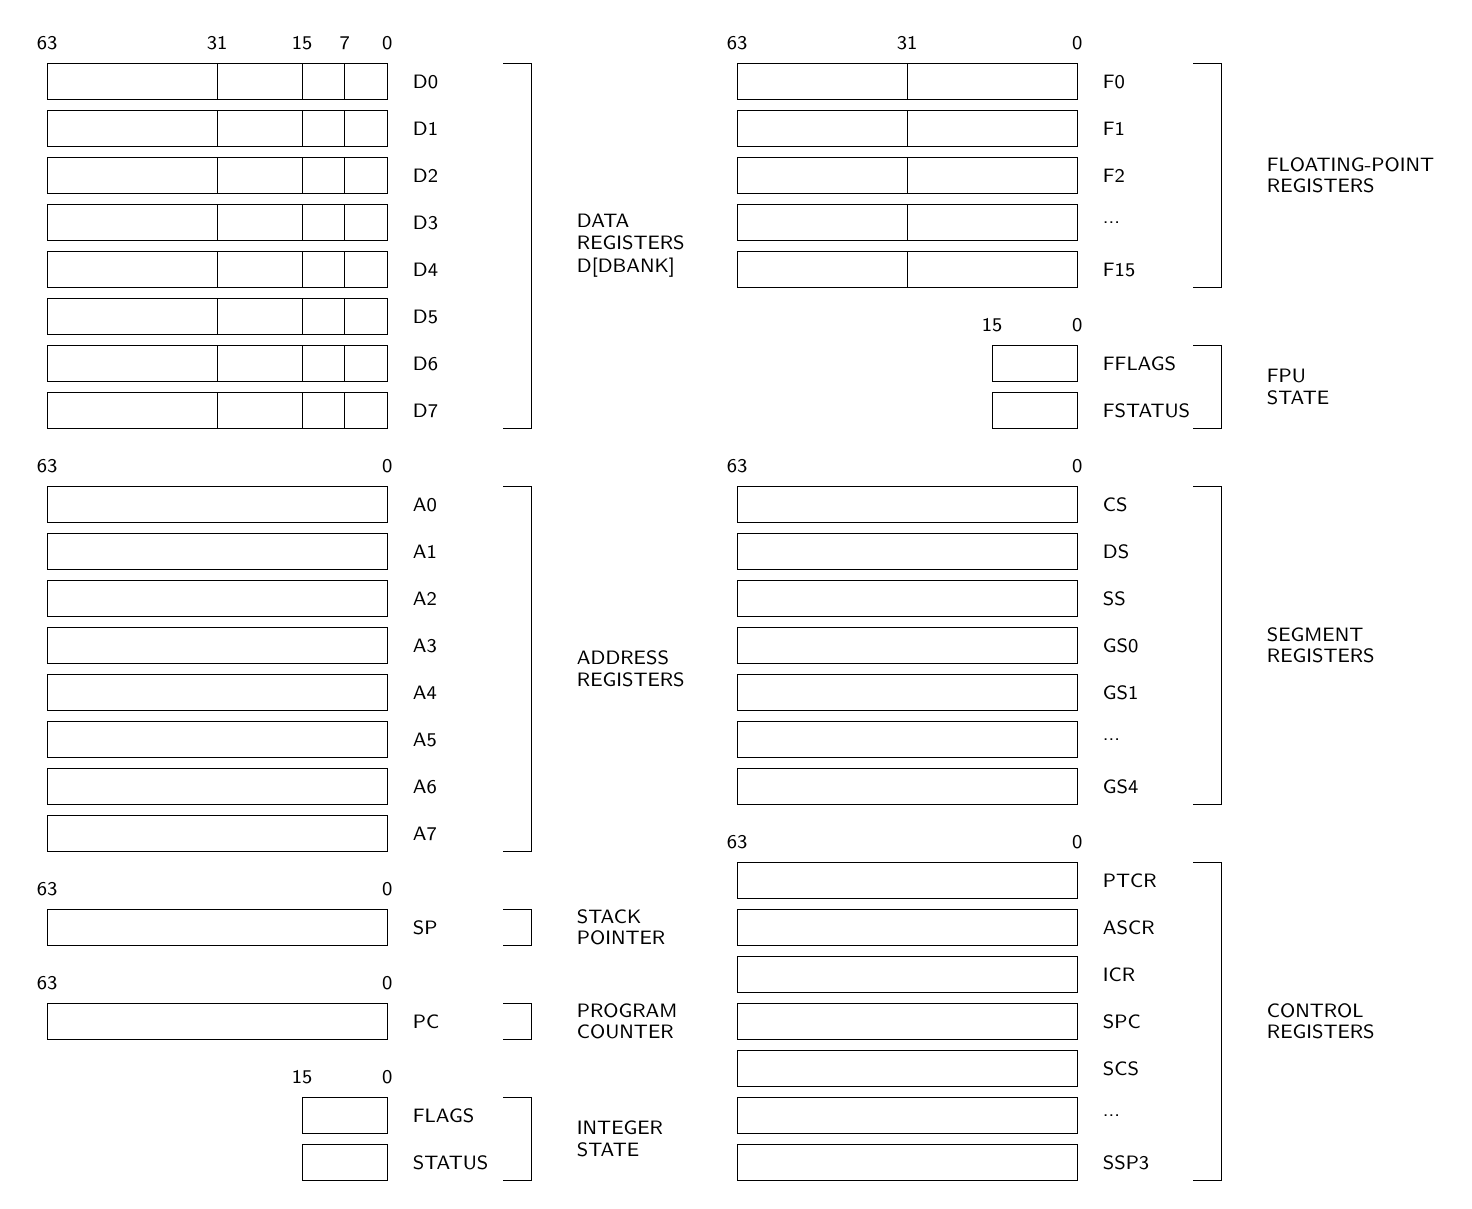
\begin{tikzpicture}[x=1in,y=1in,every node/.style={font=\scriptsize}]
\def\regw{1.70}
\def\rowh{0.18}
\def\gap{0.055}
\node[anchor=south] at (0.000,0.020) {63};
\node[anchor=south] at (0.850,0.020) {31};
\node[anchor=south] at (1.275,0.020) {15};
\node[anchor=south] at (1.488,0.020) {7};
\node[anchor=south] at (1.700,0.020) {0};
\draw (0.000,-0.180) rectangle (1.700,0.000);
\draw (0.850,-0.180) -- (0.850,0.000);
\draw (1.275,-0.180) -- (1.275,0.000);
\draw (1.488,-0.180) -- (1.488,0.000);
\node[anchor=west] at (1.780,-0.090) {D0};
\draw (0.000,-0.415) rectangle (1.700,-0.235);
\draw (0.850,-0.415) -- (0.850,-0.235);
\draw (1.275,-0.415) -- (1.275,-0.235);
\draw (1.488,-0.415) -- (1.488,-0.235);
\node[anchor=west] at (1.780,-0.325) {D1};
\draw (0.000,-0.650) rectangle (1.700,-0.470);
\draw (0.850,-0.650) -- (0.850,-0.470);
\draw (1.275,-0.650) -- (1.275,-0.470);
\draw (1.488,-0.650) -- (1.488,-0.470);
\node[anchor=west] at (1.780,-0.560) {D2};
\draw (0.000,-0.885) rectangle (1.700,-0.705);
\draw (0.850,-0.885) -- (0.850,-0.705);
\draw (1.275,-0.885) -- (1.275,-0.705);
\draw (1.488,-0.885) -- (1.488,-0.705);
\node[anchor=west] at (1.780,-0.795) {D3};
\draw (0.000,-1.120) rectangle (1.700,-0.940);
\draw (0.850,-1.120) -- (0.850,-0.940);
\draw (1.275,-1.120) -- (1.275,-0.940);
\draw (1.488,-1.120) -- (1.488,-0.940);
\node[anchor=west] at (1.780,-1.030) {D4};
\draw (0.000,-1.355) rectangle (1.700,-1.175);
\draw (0.850,-1.355) -- (0.850,-1.175);
\draw (1.275,-1.355) -- (1.275,-1.175);
\draw (1.488,-1.355) -- (1.488,-1.175);
\node[anchor=west] at (1.780,-1.265) {D5};
\draw (0.000,-1.590) rectangle (1.700,-1.410);
\draw (0.850,-1.590) -- (0.850,-1.410);
\draw (1.275,-1.590) -- (1.275,-1.410);
\draw (1.488,-1.590) -- (1.488,-1.410);
\node[anchor=west] at (1.780,-1.500) {D6};
\draw (0.000,-1.825) rectangle (1.700,-1.645);
\draw (0.850,-1.825) -- (0.850,-1.645);
\draw (1.275,-1.825) -- (1.275,-1.645);
\draw (1.488,-1.825) -- (1.488,-1.645);
\node[anchor=west] at (1.780,-1.735) {D7};
\draw (2.280,0.000) -- (2.420,0.000) -- (2.420,-1.825) -- (2.280,-1.825);
\node[anchor=west] at (2.600,-0.912) {\shortstack[l]{DATA\\REGISTERS\\D[DBANK]}};
\node[anchor=south] at (0.000,-2.095) {63};
\node[anchor=south] at (1.700,-2.095) {0};
\draw (0.000,-2.295) rectangle (1.700,-2.115);
\node[anchor=west] at (1.780,-2.205) {A0};
\draw (0.000,-2.530) rectangle (1.700,-2.350);
\node[anchor=west] at (1.780,-2.440) {A1};
\draw (0.000,-2.765) rectangle (1.700,-2.585);
\node[anchor=west] at (1.780,-2.675) {A2};
\draw (0.000,-3.000) rectangle (1.700,-2.820);
\node[anchor=west] at (1.780,-2.910) {A3};
\draw (0.000,-3.235) rectangle (1.700,-3.055);
\node[anchor=west] at (1.780,-3.145) {A4};
\draw (0.000,-3.470) rectangle (1.700,-3.290);
\node[anchor=west] at (1.780,-3.380) {A5};
\draw (0.000,-3.705) rectangle (1.700,-3.525);
\node[anchor=west] at (1.780,-3.615) {A6};
\draw (0.000,-3.940) rectangle (1.700,-3.760);
\node[anchor=west] at (1.780,-3.850) {A7};
\draw (2.280,-2.115) -- (2.420,-2.115) -- (2.420,-3.940) -- (2.280,-3.940);
\node[anchor=west] at (2.600,-3.027) {\shortstack[l]{ADDRESS\\REGISTERS}};
\node[anchor=south] at (0.000,-4.210) {63};
\node[anchor=south] at (1.700,-4.210) {0};
\draw (0.000,-4.410) rectangle (1.700,-4.230);
\node[anchor=west] at (1.780,-4.320) {SP};
\draw (2.280,-4.230) -- (2.420,-4.230) -- (2.420,-4.410) -- (2.280,-4.410);
\node[anchor=west] at (2.600,-4.320) {\shortstack[l]{STACK\\POINTER}};
\node[anchor=south] at (0.000,-4.680) {63};
\node[anchor=south] at (1.700,-4.680) {0};
\draw (0.000,-4.880) rectangle (1.700,-4.700);
\node[anchor=west] at (1.780,-4.790) {PC};
\draw (2.280,-4.700) -- (2.420,-4.700) -- (2.420,-4.880) -- (2.280,-4.880);
\node[anchor=west] at (2.600,-4.790) {\shortstack[l]{PROGRAM\\COUNTER}};
\node[anchor=south] at (1.275,-5.150) {15};
\node[anchor=south] at (1.700,-5.150) {0};
\draw (1.275,-5.350) rectangle (1.700,-5.170);
\node[anchor=west] at (1.780,-5.260) {FLAGS};
\draw (1.275,-5.585) rectangle (1.700,-5.405);
\node[anchor=west] at (1.780,-5.495) {STATUS};
\draw (2.280,-5.170) -- (2.420,-5.170) -- (2.420,-5.585) -- (2.280,-5.585);
\node[anchor=west] at (2.600,-5.377) {\shortstack[l]{INTEGER\\STATE}};
\node[anchor=south] at (3.450,0.020) {63};
\node[anchor=south] at (4.300,0.020) {31};
\node[anchor=south] at (5.150,0.020) {0};
\draw (3.450,-0.180) rectangle (5.150,0.000);
\draw (4.300,-0.180) -- (4.300,0.000);
\node[anchor=west] at (5.230,-0.090) {F0};
\draw (3.450,-0.415) rectangle (5.150,-0.235);
\draw (4.300,-0.415) -- (4.300,-0.235);
\node[anchor=west] at (5.230,-0.325) {F1};
\draw (3.450,-0.650) rectangle (5.150,-0.470);
\draw (4.300,-0.650) -- (4.300,-0.470);
\node[anchor=west] at (5.230,-0.560) {F2};
\draw (3.450,-0.885) rectangle (5.150,-0.705);
\draw (4.300,-0.885) -- (4.300,-0.705);
\node[anchor=west] at (5.230,-0.795) {...};
\draw (3.450,-1.120) rectangle (5.150,-0.940);
\draw (4.300,-1.120) -- (4.300,-0.940);
\node[anchor=west] at (5.230,-1.030) {F15};
\draw (5.730,0.000) -- (5.870,0.000) -- (5.870,-1.120) -- (5.730,-1.120);
\node[anchor=west] at (6.050,-0.560) {\shortstack[l]{FLOATING-POINT\\REGISTERS}};
\node[anchor=south] at (4.725,-1.390) {15};
\node[anchor=south] at (5.150,-1.390) {0};
\draw (4.725,-1.590) rectangle (5.150,-1.410);
\node[anchor=west] at (5.230,-1.500) {FFLAGS};
\draw (4.725,-1.825) rectangle (5.150,-1.645);
\node[anchor=west] at (5.230,-1.735) {FSTATUS};
\draw (5.730,-1.410) -- (5.870,-1.410) -- (5.870,-1.825) -- (5.730,-1.825);
\node[anchor=west] at (6.050,-1.617) {\shortstack[l]{FPU\\STATE}};
\node[anchor=south] at (3.450,-2.095) {63};
\node[anchor=south] at (5.150,-2.095) {0};
\draw (3.450,-2.295) rectangle (5.150,-2.115);
\node[anchor=west] at (5.230,-2.205) {CS};
\draw (3.450,-2.530) rectangle (5.150,-2.350);
\node[anchor=west] at (5.230,-2.440) {DS};
\draw (3.450,-2.765) rectangle (5.150,-2.585);
\node[anchor=west] at (5.230,-2.675) {SS};
\draw (3.450,-3.000) rectangle (5.150,-2.820);
\node[anchor=west] at (5.230,-2.910) {GS0};
\draw (3.450,-3.235) rectangle (5.150,-3.055);
\node[anchor=west] at (5.230,-3.145) {GS1};
\draw (3.450,-3.470) rectangle (5.150,-3.290);
\node[anchor=west] at (5.230,-3.380) {...};
\draw (3.450,-3.705) rectangle (5.150,-3.525);
\node[anchor=west] at (5.230,-3.615) {GS4};
\draw (5.730,-2.115) -- (5.870,-2.115) -- (5.870,-3.705) -- (5.730,-3.705);
\node[anchor=west] at (6.050,-2.910) {\shortstack[l]{SEGMENT\\REGISTERS}};
\node[anchor=south] at (3.450,-3.975) {63};
\node[anchor=south] at (5.150,-3.975) {0};
\draw (3.450,-4.175) rectangle (5.150,-3.995);
\node[anchor=west] at (5.230,-4.085) {PTCR};
\draw (3.450,-4.410) rectangle (5.150,-4.230);
\node[anchor=west] at (5.230,-4.320) {ASCR};
\draw (3.450,-4.645) rectangle (5.150,-4.465);
\node[anchor=west] at (5.230,-4.555) {ICR};
\draw (3.450,-4.880) rectangle (5.150,-4.700);
\node[anchor=west] at (5.230,-4.790) {SPC};
\draw (3.450,-5.115) rectangle (5.150,-4.935);
\node[anchor=west] at (5.230,-5.025) {SCS};
\draw (3.450,-5.350) rectangle (5.150,-5.170);
\node[anchor=west] at (5.230,-5.260) {...};
\draw (3.450,-5.585) rectangle (5.150,-5.405);
\node[anchor=west] at (5.230,-5.495) {SSP3};
\draw (5.730,-3.995) -- (5.870,-3.995) -- (5.870,-5.585) -- (5.730,-5.585);
\node[anchor=west] at (6.050,-4.790) {\shortstack[l]{CONTROL\\REGISTERS}};
\end{tikzpicture}
}
\manualfigurecaption{User Programming Model}
\end{center}


\begin{manualtabular}{@{}>{\raggedright\arraybackslash}p{0.7in}>{\raggedright\arraybackslash}p{0.65in}>{\raggedright\arraybackslash}p{0.65in}>{\raggedright\arraybackslash}p{1.45in}>{\raggedright\arraybackslash}p{1.2in}@{}}
\toprule
\textbf{Class} & \textbf{Count} & \textbf{Width} & \textbf{Role} & \textbf{Allocatable}\\
\midrule
\texttt{D} & 8 & 64 & data & True\\
\texttt{A} & 8 & 64 & address & True\\
\texttt{SP} & 1 & 64 & stack pointer & False\\
\texttt{PC} & 1 & 64 & program counter & False\\
\texttt{F} & 16 & 64 & floating-point & True\\
\texttt{S} & 8 & 64 & segment & False\\
\texttt{CR} & 18 & 64 & control & False\\
\bottomrule
\end{manualtabular}
\manualtablecaption{Register Classes}


\subsection{Data Register Banks}
D-register banking extends the data-register file without changing the 3-bit DREG fields used by ordinary
instructions. The current DBANK selector chooses which physical D0 through D7 bank is visible.
Source-language ABIs do not expose DBANK; compilers, runtimes, hand-written assembly, and repeat/block
optimizers may use nonzero banks when the target profile provides them.

\begin{manuallongtable}{@{}>{\raggedright\arraybackslash}p{1.55in}>{\raggedright\arraybackslash}p{3.95in}@{}}
\toprule
\textbf{Property} & \textbf{Value}\\
\midrule
\endhead
Selector & \texttt{DBANK}\\
Selector width & 4 bits\\
Architectural namespace & 16 banks\\
Base required count & 1\\
Discovery & CPUID implementation properties.DATA\_REGISTER\_BANKS\\
Object attribute & \texttt{BEDROCK\_ATTR\_REQUIRED\_DBANK\_COUNT}\\
\bottomrule
\end{manuallongtable}
\manualtablecaption{Data Register Bank Selector}


\begin{manuallongtable}{@{}>{\raggedright\arraybackslash}p{1.55in}>{\raggedright\arraybackslash}p{3.95in}@{}}
\toprule
\textbf{Rule} & \textbf{Meaning}\\
\midrule
\endhead
Visible D register & \texttt{Dn names D[DBANK][n]}\\
Ordinary D operands & ordinary DREG operands use the current DBANK selector\\
Bank 0 & ABI-visible data-register bank\\
Public ABI boundary & DBANK must be 0 at public ABI boundaries\\
Handler entry & exception, interrupt, trap, and syscall handlers save the interrupted DBANK selector and execute with DBANK set to 0\\
Saved state & supervisor-entry and syscall frames save the interrupted DBANK selector; IRET and SYSRET restore it from the saved frame image\\
\bottomrule
\end{manuallongtable}
\manualtablecaption{Data Register Bank Rules}


\begin{manuallongtable}{@{}>{\raggedright\arraybackslash}p{0.85in}>{\raggedright\arraybackslash}p{0.65in}>{\raggedright\arraybackslash}p{4.00in}@{}}
\toprule
\textbf{Tier} & \textbf{Banks} & \textbf{Meaning}\\
\midrule
\endhead
\texttt{DBANK1} & 1 & only bank 0 is implemented; bank-switching instructions exist but nonzero bank selectors fault\\
\texttt{DBANK4} & 4 & banks 0 through 3 are available for backend and runtime scratch allocation\\
\texttt{DBANK16} & 16 & the full 4-bit architectural bank namespace is available\\
\bottomrule
\end{manuallongtable}
\manualtablecaption{Data Register Bank Availability Tiers}



\subsection{FLAGS and STATUS Registers}
FLAGS and STATUS are accessed through dedicated 16-bit W-sized read/write instructions, not through the S
segment-register operand class. Reserved bits read as zero and must remain zero; FLAGS has four meaningful
bits and STATUS has 6 meaningful bits.

\begin{manuallistedformatdiagram}{FLAGS Register Format}{3}
\manualformatrow{FLAGS[15:0]}{%
\manualformatfield{0}{12}
\manualformatfield{Z}{1}
\manualformatfield{N}{1}
\manualformatfield{C}{1}
\manualformatfield{V}{1}
}
\end{manuallistedformatdiagram}


\begin{manuallongtable}{@{}>{\raggedright\arraybackslash}p{0.55in}>{\raggedright\arraybackslash}p{0.65in}>{\raggedright\arraybackslash}p{4.05in}@{}}
\toprule
\textbf{Bit} & \textbf{Position} & \textbf{Meaning}\\
\midrule
\endhead
\texttt{Z} & 3 & zero\\
\texttt{N} & 2 & negative\\
\texttt{C} & 1 & carry or borrow\\
\texttt{V} & 0 & overflow\\
\bottomrule
\end{manuallongtable}
\manualtablecaption{FLAGS Bits}


\begin{manuallistedformatdiagram}{STATUS Register Format}{3}
\manualformatrow{STATUS[15:0]}{%
\manualformatfield{0}{10}
\manualformatfield{IE}{1}
\manualformatfield{PM}{1}
\manualformatfield{RF}{1}
\manualformatfield{TF}{1}
\manualformatfield{NI}{1}
\manualformatfield{IN}{1}
}
\end{manuallistedformatdiagram}


\begin{manuallongtable}{@{}>{\raggedright\arraybackslash}p{0.55in}>{\raggedright\arraybackslash}p{0.65in}>{\raggedright\arraybackslash}p{4.05in}@{}}
\toprule
\textbf{Bit} & \textbf{Position} & \textbf{Meaning}\\
\midrule
\endhead
\texttt{IE} & 5 & interrupt enable\\
\texttt{PM} & 4 & privileged mode; 0 = user, 1 = supervisor\\
\texttt{RF} & 3 & resume flag\\
\texttt{TF} & 2 & trap flag\\
\texttt{NI} & 1 & NMI in-progress\\
\texttt{IN} & 0 & interrupt nesting enable\\
\bottomrule
\end{manuallongtable}
\manualtablecaption{STATUS Bits}



\subsection{Floating-Point Register Model}
The floating-point extension defines 16 Q-sized floating-point registers, F0-F15.
Single-precision and double-precision operations use the same register file. FFLAGS holds accrued
floating-point exception flags. FSTATUS holds floating-point control and status-mode state, including
trap enables, rounding mode, and non-default arithmetic modes.

\begin{manualtabular}{@{}>{\raggedright\arraybackslash}p{1.55in}>{\raggedright\arraybackslash}p{3.95in}@{}}
\toprule
\textbf{Property} & \textbf{Value}\\
\midrule
Registers & \texttt{F0-F15}\\
Count & 16\\
Architectural width & 64 bits\\
Scalar formats & S, D\\
FFLAGS width & 16 bits\\
FSTATUS width & 16 bits\\
FFLAGS reset & \texttt{0}\\
FSTATUS reset & \texttt{0}\\
Unsupported extension instruction & \texttt{ILLEGAL\_INSTRUCTION}\\
\bottomrule
\end{manualtabular}
\manualtablecaption{Floating-Point Register File}


\begin{manualtabular}{@{}>{\raggedright\arraybackslash}p{0.55in}>{\raggedright\arraybackslash}p{0.65in}>{\raggedright\arraybackslash}p{4.05in}@{}}
\toprule
\textbf{Bit} & \textbf{Position} & \textbf{Meaning}\\
\midrule
\texttt{NV} & 4 & accrued invalid operation flag\\
\texttt{DZ} & 3 & accrued divide-by-zero flag\\
\texttt{OF} & 2 & accrued overflow flag\\
\texttt{UF} & 1 & accrued underflow flag\\
\texttt{NX} & 0 & accrued inexact flag\\
\bottomrule
\end{manualtabular}
\manualtablecaption{FFLAGS Bits}


\begin{manualtabular}{@{}>{\raggedright\arraybackslash}p{0.85in}>{\raggedright\arraybackslash}p{0.75in}>{\raggedright\arraybackslash}p{3.90in}@{}}
\toprule
\textbf{Field} & \textbf{Position} & \textbf{Meaning}\\
\midrule
\texttt{NV\_EN} & 4 & invalid operation trap enable\\
\texttt{DZ\_EN} & 3 & divide-by-zero trap enable\\
\texttt{OF\_EN} & 2 & overflow trap enable\\
\texttt{UF\_EN} & 1 & underflow trap enable\\
\texttt{NX\_EN} & 0 & inexact trap enable\\
\texttt{RM} & 6:5 & rounding mode\\
\texttt{FTZ} & 7 & flush tiny results to signed zero\\
\texttt{DAZ} & 8 & treat subnormal inputs as signed zero\\
\texttt{DN} & 9 & default NaN result mode\\
\texttt{reserved} & 15:10 & reserved, must be zero\\
\bottomrule
\end{manualtabular}
\manualtablecaption{FSTATUS Fields}


\begin{manualtabular}{@{}>{\raggedright\arraybackslash}p{0.65in}>{\raggedright\arraybackslash}p{4.85in}@{}}
\toprule
\textbf{Value} & \textbf{Rounding Mode}\\
\midrule
\texttt{0} & roundTiesToEven\\
\texttt{1} & roundTowardZero\\
\texttt{2} & roundTowardNegative\\
\texttt{3} & roundTowardPositive\\
\bottomrule
\end{manualtabular}
\manualtablecaption{FSTATUS Rounding Modes}


\begin{itemize}[leftmargin=1.4em,itemsep=1pt,topsep=2pt]\raggedright
\item Set the corresponding accrued FFLAGS bit and continue.
\item Raise FLOATING\_POINT\_FAULT when the corresponding exception occurs.
\item Reserved FSTATUS bits must be zero; nonzero reserved writes raise INVALID\_CONTROL\_STATE.
\item FSTATUS=0 selects roundTiesToEven, disables exception traps, and leaves FTZ, DAZ, and DN disabled
\end{itemize}


\Needspace{3.8in}
\subsection{Segment Registers}
Segment registers define a currently addressable memory window plus a simple
address translation step. They are not the memory-protection mechanism; paging
supplies memory access permissions and final address translation. When the
segment mantissa field is zero, the segment entry is disabled. When the mantissa
is nonzero, an address passes through segmentation first and then through
paging.

The bounds-only bit enables a check-only mode for segment translation: the
segment bounds are tested, but the segment base address is not added to the
translated address.

\begin{manuallongtable}{@{}>{\raggedright\arraybackslash}p{0.75in}>{\raggedright\arraybackslash}p{1.1in}>{\raggedright\arraybackslash}p{0.65in}@{}}
\toprule
\textbf{Register} & \textbf{Selector} & \textbf{Width}\\
\midrule
\endhead
\texttt{CS} & code & 64\\
\texttt{DS} & data & 64\\
\texttt{SS} & stack & 64\\
\texttt{GS0} & general & 64\\
\texttt{GS1} & general & 64\\
\texttt{GS2} & general & 64\\
\texttt{GS3} & general & 64\\
\texttt{GS4} & general & 64\\
\bottomrule
\end{manuallongtable}
\manualtablecaption{Segment Registers}


\begin{manuallistedformatdiagram}{Segment Register Format}{5}
\manualformatrow{segment[63:0]}{%
\manualformatfield{base\_page}{52}
\manualformatfield{e}{5}
\manualformatfield{m}{6}
\manualformatfield{b}{1}
}
\end{manuallistedformatdiagram}


\begin{manuallongtable}{@{}>{\raggedright\arraybackslash}p{0.85in}>{\raggedright\arraybackslash}p{0.65in}>{\raggedright\arraybackslash}p{3.75in}@{}}
\toprule
\textbf{Field} & \textbf{Bits} & \textbf{Meaning}\\
\midrule
\endhead
\texttt{base\_page} & 63:12 & page-unit segment base index\\
\texttt{e} & 11:7 & segment size exponent\\
\texttt{m} & 6:1 & segment size mantissa\\
\texttt{b} & 0 & bounds-only mode enable; check segment bounds without adding the segment base address\\
\bottomrule
\end{manuallongtable}
\manualtablecaption{Segment Register Fields}


\begin{align*}
\text{base byte address} &= \mathit{base\_page} \times 4096\\
\text{segment size} &= m \times 2^e \times 4096\\
\text{limit byte address} &= (\mathit{base\_page} + m \times 2^e) \times 4096\\
b=0:\quad \text{segmented address} &= \text{base byte address} + \text{offset},\quad 0 \le \text{offset} < \text{segment size}\\
b=1:\quad \text{segmented address} &= \text{offset},\quad \text{base byte address} \le \text{offset} < \text{limit byte address}
\end{align*}

The base, segment size, and limit are computed in an unsigned domain wide
enough to represent the full 64-bit linear-address space plus one. If the limit
exceeds \(2^{64}\), the segment register image is invalid and any access through
it reports \texttt{PAGE\_FAULT}.

If m is zero, segmentation is disabled for that segment selector and the
effective address is already the linear address. If m is nonzero, the segment
bounds are checked before paging. In normal mode (b = 0), the segment base is
added to the offset after the bounds check. In bounds-only mode (b = 1), the
base is not added; the segment only constrains which linear-address window may
be accessed.


\subsection{Segment Register Operand Class}
The S class is the Q-sized segment-register operand class used by RDSEG and WRSEG. Its selector values
are defined by the SREG selector table. SS is distinct from the SP stack-pointer register, and FLAGS and
STATUS are accessed through dedicated RD/WR instructions.

\begin{manuallongtable}{@{}>{\raggedright\arraybackslash}p{0.55in}>{\raggedright\arraybackslash}p{0.55in}>{\raggedright\arraybackslash}p{0.45in}>{\raggedright\arraybackslash}p{1.05in}>{\raggedright\arraybackslash}p{2.8in}@{}}
\toprule
\textbf{Class} & \textbf{Width} & \textbf{Bits} & \textbf{Role} & \textbf{Registers}\\
\midrule
\endhead
\texttt{S} & 64 & 3 & segment & \begin{tabular}[t]{@{}l@{}}CS\\DS\\SS\\GS0\\GS1\\GS2\\GS3\\GS4\end{tabular}\\
\bottomrule
\end{manuallongtable}
\manualtablecaption{Segment Register Operand Class}


\begin{manuallongtable}{@{}>{\raggedright\arraybackslash}p{0.55in}>{\raggedright\arraybackslash}p{1.0in}>{\raggedright\arraybackslash}p{3.90in}@{}}
\toprule
\textbf{Bits} & \textbf{Register} & \textbf{Reserved Access}\\
\midrule
\endhead
\texttt{000} & \texttt{CS} & -\\
\texttt{001} & \texttt{DS} & -\\
\texttt{010} & \texttt{SS} & -\\
\texttt{011} & \texttt{GS0} & -\\
\texttt{100} & \texttt{GS1} & -\\
\texttt{101} & \texttt{GS2} & -\\
\texttt{110} & \texttt{GS3} & -\\
\texttt{111} & \texttt{GS4} & -\\
\bottomrule
\end{manuallongtable}
\manualtablecaption{RDSEG/WRSEG Segment Register Selector Encoding}



\subsection{Special Registers}
\begin{manuallongtable}{@{}>{\raggedright\arraybackslash}p{0.7in}>{\raggedright\arraybackslash}p{0.5in}>{\raggedright\arraybackslash}p{0.5in}>{\raggedright\arraybackslash}p{0.8in}>{\raggedright\arraybackslash}p{0.9in}>{\raggedright\arraybackslash}p{0.65in}@{}}
\toprule
\textbf{Name} & \textbf{Width} & \textbf{Class} & \textbf{Role} & \textbf{Privilege} & \textbf{Implicit}\\
\midrule
\endhead
\texttt{PC} & 64 & PC & - & any & True\\
\texttt{SP} & 64 & SP & - & any & True\\
\texttt{FLAGS} & 16 & FLAGS & condition flags & any & True\\
\texttt{STATUS} & 16 & STATUS & state & supervisor & False\\
\texttt{FSTATUS} & 16 & FSTATUS & floating-point control and status mode & unprivileged & False\\
\texttt{FFLAGS} & 16 & FFLAGS & floating-point accrued exception flags & unprivileged & False\\
\bottomrule
\end{manuallongtable}
\manualtablecaption{Special Registers}


\subsection{Control Registers}
Control registers are Q-sized privileged registers used for translation, interrupt, boot, counter, and
privileged-entry state. PTCR and ASCR configure the memory-address translation pipeline described in the
Memory Address Translation section; ICR configures interrupt-vector state; SPC, SCS, and SDS hold
supervisor-entry control state.

\begin{manualtabular}{@{}>{\raggedright\arraybackslash}p{1.05in}>{\raggedright\arraybackslash}p{1.0in}>{\raggedright\arraybackslash}p{0.55in}>{\raggedright\arraybackslash}p{0.85in}>{\raggedright\arraybackslash}p{2.10in}@{}}
\toprule
\textbf{Group} & \textbf{Register(s)} & \textbf{Width} & \textbf{Privilege} & \textbf{Role}\\
\midrule
translation & \begin{tabular}[t]{@{}l@{}}\texttt{PTCR}\\\texttt{ASCR}\\\texttt{ICR}\end{tabular} & 64 & supervisor & \begin{tabular}[t]{@{}l@{}}control\\control\\control\end{tabular}\\
supervisor entry & \begin{tabular}[t]{@{}l@{}}\texttt{SPC}\\\texttt{SCS}\\\texttt{SDS}\end{tabular} & 64 & supervisor & \begin{tabular}[t]{@{}l@{}}supervisor entry program counter\\supervisor entry code segment selector\\supervisor entry data segment selector\end{tabular}\\
interrupt stack banks & \begin{tabular}[t]{@{}l@{}}\texttt{SSS0}\\\texttt{SSP0}\\\texttt{SSS1}\\\texttt{SSP1}\\\texttt{SSS2}\\\texttt{SSP2}\\\texttt{SSS3}\\\texttt{SSP3}\end{tabular} & 64 & supervisor & \begin{tabular}[t]{@{}l@{}}interrupt stack segment selector bank 0\\interrupt stack pointer bank 0\\interrupt stack segment selector bank 1\\interrupt stack pointer bank 1\\interrupt stack segment selector bank 2\\interrupt stack pointer bank 2\\interrupt stack segment selector bank 3\\interrupt stack pointer bank 3\end{tabular}\\
boot & \begin{tabular}[t]{@{}l@{}}\texttt{BOOTPC}\\\texttt{BOOTCFG}\end{tabular} & 64 & supervisor & \begin{tabular}[t]{@{}l@{}}control\\control\end{tabular}\\
counters & \begin{tabular}[t]{@{}l@{}}\texttt{PTC}\\\texttt{PMC}\end{tabular} & 64 & supervisor & \begin{tabular}[t]{@{}l@{}}control\\control\end{tabular}\\
\bottomrule
\end{manualtabular}
\manualtablecaption{Control Registers}


RDCR and WRCR use 16-bit control-register selectors. Selectors are grouped by function, leaving space
inside each group for related control state.

\begin{manualtabular}{@{}>{\raggedright\arraybackslash}p{1.35in}>{\raggedright\arraybackslash}p{4.15in}@{}}
\toprule
\textbf{Group} & \textbf{Selector / Register}\\
\midrule
translation & \begin{tabular}[t]{@{}l@{}}\texttt{0x0000} \texttt{PTCR}\\\texttt{0x0001} \texttt{ASCR}\\\texttt{0x0002} \texttt{ICR}\end{tabular}\\
supervisor entry & \begin{tabular}[t]{@{}l@{}}\texttt{0x0100} \texttt{SPC}\\\texttt{0x0101} \texttt{SCS}\\\texttt{0x0102} \texttt{SDS}\end{tabular}\\
interrupt stack banks & \begin{tabular}[t]{@{}l@{}}\texttt{0x0200} \texttt{SSS0}\\\texttt{0x0201} \texttt{SSP0}\\\texttt{0x0210} \texttt{SSS1}\\\texttt{0x0211} \texttt{SSP1}\\\texttt{0x0220} \texttt{SSS2}\\\texttt{0x0221} \texttt{SSP2}\\\texttt{0x0230} \texttt{SSS3}\\\texttt{0x0231} \texttt{SSP3}\end{tabular}\\
boot & \begin{tabular}[t]{@{}l@{}}\texttt{0x1000} \texttt{BOOTPC}\\\texttt{0x1001} \texttt{BOOTCFG}\end{tabular}\\
counters & \begin{tabular}[t]{@{}l@{}}\texttt{0x1100} \texttt{PTC}\\\texttt{0x1101} \texttt{PMC}\end{tabular}\\
unassigned & \begin{tabular}[t]{@{}l@{}}all other selectors\\\texttt{INVALID\_CONTROL\_STATE}\end{tabular}\\
\bottomrule
\end{manualtabular}
\manualtablecaption{Control Register Selector Encoding}


\begin{manuallistedformatdiagram}{PTCR Format}{8}
\manualformatrow{PTCR[63:0]}{%
\manualformatfield{root\_page}{52}
\manualformatfield{PABITS}{5}
\manualformatfield{LA57}{1}
\manualformatfield{reserved}{5}
\manualformatfield{PE}{1}
}
\end{manuallistedformatdiagram}


\begin{manuallongtable}{@{}>{\raggedright\arraybackslash}p{0.95in}>{\raggedright\arraybackslash}p{0.65in}>{\raggedright\arraybackslash}p{3.85in}@{}}
\toprule
\textbf{Field} & \textbf{Bits} & \textbf{Meaning}\\
\midrule
\endhead
\texttt{root\_page} & 63:12 & page-table root physical frame number\\
\texttt{PABITS\_SEL} & 11:8 & physical address width selector\\
\texttt{LA57} & 7 & 5-level paging enable\\
\texttt{reserved} & 6:1 & reserved, must be zero\\
\texttt{PE} & 0 & page-table translation enable\\
\bottomrule
\end{manuallongtable}
\manualtablecaption{PTCR Fields}


\begin{manuallongtable}{@{}>{\raggedright\arraybackslash}p{0.80in}>{\raggedright\arraybackslash}p{0.85in}>{\raggedright\arraybackslash}p{3.85in}@{}}
\toprule
\textbf{Selector} & \textbf{PABITS} & \textbf{Reserved Access}\\
\midrule
\endhead
\texttt{0} & 48 & -\\
\texttt{1} & 56 & -\\
\texttt{2..15} & reserved & \texttt{INVALID\_CONTROL\_STATE}\\
\bottomrule
\end{manuallongtable}
\manualtablecaption{PTCR PABITS Selector Encoding}


\begin{manuallistedformatdiagram}{ASCR Format}{8}
\manualformatrow{ASCR[63:0]}{%
\manualformatfield{reserved}{32}
\manualformatfield{ASID}{16}
\manualformatfield{reserved}{15}
\manualformatfield{AE}{1}
}
\end{manuallistedformatdiagram}


ASCR holds the current address-space identifier. SWPT Dn performs a page-table swap that clears ASCR.
SWPTA Dn, Dn performs a context-aware page-table swap: PTCR is updated, ASCR[31:16] is set from the
low 16 bits of the second data-register operand, and ASCR.AE is set.

\begin{manuallongtable}{@{}>{\raggedright\arraybackslash}p{0.95in}>{\raggedright\arraybackslash}p{0.65in}>{\raggedright\arraybackslash}p{3.85in}@{}}
\toprule
\textbf{Field} & \textbf{Bits} & \textbf{Meaning}\\
\midrule
\endhead
\texttt{reserved\_high} & 63:32 & reserved, must be zero\\
\texttt{ASID} & 31:16 & current address-space identifier\\
\texttt{reserved\_low} & 15:1 & reserved, must be zero\\
\texttt{AE} & 0 & ASID enable\\
\bottomrule
\end{manuallongtable}
\manualtablecaption{ASCR Fields}


\begin{manuallistedformatdiagram}{ICR Format}{8}
\manualformatrow{ICR[63:0]}{%
\manualformatfield{ivt\_page}{52}
\manualformatfield{MAX\_IDEPTH}{5}
\manualformatfield{NMI\_P}{1}
\manualformatfield{NMI\_L}{1}
\manualformatfield{DF}{1}
\manualformatfield{reserved}{3}
\manualformatfield{V}{1}
}
\end{manuallistedformatdiagram}


\begin{manuallongtable}{@{}>{\raggedright\arraybackslash}p{0.95in}>{\raggedright\arraybackslash}p{0.65in}>{\raggedright\arraybackslash}p{3.85in}@{}}
\toprule
\textbf{Field} & \textbf{Bits} & \textbf{Meaning}\\
\midrule
\endhead
\texttt{ivt\_page} & 63:12 & interrupt vector table frame number / page number\\
\texttt{MAX\_IDEPTH} & 11:8 & maximum maskable interrupt nesting depth\\
\texttt{NMI\_PENDING} & 7 & hardware-managed NMI pending bit\\
\texttt{NMI\_LATCH} & 6 & latch NMI while STATUS.NI is set\\
\texttt{DF\_ENABLE} & 5 & double-fault handling enable\\
\texttt{reserved} & 4:1 & reserved, must be zero\\
\texttt{IVT\_VALID} & 0 & interrupt vector table valid\\
\bottomrule
\end{manuallongtable}
\manualtablecaption{ICR Fields}


The detailed interrupt-vector and supervisor-entry frame layouts are described in the Exception Processing
Reference section.


\clearpage
\section{CPUID Feature Discovery}
\subsection{Overview}
CPUID is the architectural discovery instruction. It exposes base-profile identity, optional
architectural extensions, and program-visible tuning properties. It is not a dump of internal
microarchitectural structures.

A leaf describes one meaningful information group. The result index selects one Q-sized result
from that group.

\subsection{Query Model}
The instruction form is \texttt{CPUID Dn}. The selected D register contains a 64-bit query selector
before execution and receives the selected 64-bit result after execution. The selector is divided into
a 32-bit class, a 16-bit leaf within that class, and a 16-bit result index.

\begin{manuallongtable}{@{}>{\raggedright\arraybackslash}p{1.60in}>{\raggedright\arraybackslash}p{3.85in}@{}}
\toprule
\textbf{Property} & \textbf{Spec Value}\\
\midrule
\endhead
input & Dn contains the CPUID query selector\\
output & Dn receives one selected 64-bit result\\
unsupported class & result = 0\\
unsupported leaf & result = 0\\
unsupported index & result = 0\\
privilege & unprivileged\\
serialization & not serializing\\
reserved result bits & software must ignore\\
runtime mutability & static after reset unless a leaf explicitly says otherwise\\
\bottomrule
\end{manuallongtable}
\manualtablecaption{CPUID Calling Convention}


\begin{manuallongtable}{@{}>{\raggedright\arraybackslash}p{0.70in}>{\raggedright\arraybackslash}p{1.20in}>{\raggedright\arraybackslash}p{3.60in}@{}}
\toprule
\textbf{Bits} & \textbf{Field} & \textbf{Meaning}\\
\midrule
\endhead
\texttt{0..15} & \texttt{index} & result index within the selected leaf\\
\texttt{16..31} & \texttt{leaf} & information leaf within the selected class\\
\texttt{32..63} & \texttt{class} & CPUID information class\\
\bottomrule
\end{manuallongtable}
\manualtablecaption{CPUID Query Selector}


\subsection{Discovery Classes}
\noindent\textbf{Base profile.} The base Bedrock ISA profile contains ordinary integer, data movement,
control-flow, atomic, data-register banking, cache/TLB, segmentation, paging, control-register, and
repeat-prefix instruction groups. Instruction groups with their own optional-extension leaves, such as
virtualization acceleration, are not implied by the base profile.

\noindent\textbf{Floating-point.} Floating-point discovery is intentionally coarse. An implementation reports
whether the base floating-point extension is available, and separately whether the transcendental
floating-point group is available. Double precision, fused multiply-add/subtract, floating-point
conditional move, conversion, classification, and ordinary floating-point memory/register forms are base
features of the floating-point extension.

\noindent\textbf{Data-register banking.} Data-register banking instructions are part of the base instruction set.
DBANK implementation-property discovery reports the implemented bank count and selector width; object
attributes record the minimum bank count required by a linked image. Source-language ABIs still normalize
DBANK to zero at public boundaries.

\noindent\textbf{Virtualization acceleration.} ENCINST availability is discovered through the optional-extension
class. The instruction reference groups ENCINST under Virtualization Acceleration because it supports
canonical binary emission for JITs, hypervisors, and binary translators rather than ordinary application
execution.

\noindent\textbf{Unavailable optional groups.} If an optional instruction group is not reported by CPUID,
executing an instruction from that group raises \texttt{ILLEGAL\_INSTRUCTION}. Extension availability uses the
ordinary instruction-encoding fault policy.

\noindent\textbf{Implementation properties.} Implementation-property leaves expose only information a program can
reasonably use to select code paths or tune algorithms. Structures such as register renaming, reorder buffers,
issue queues, and physical register files are not architectural discovery bits. The initial execution-property
leaf exposes only \texttt{OUT\_OF\_ORDER}. Processor-topology discovery reports the total exposed hardware-thread
count and the current hardware-thread identity; it does not report the set of CPUs currently online under an
operating system.

\begin{manuallongtable}{@{}>{\raggedright\arraybackslash}p{1.25in}>{\raggedright\arraybackslash}p{1.15in}>{\raggedright\arraybackslash}p{3.10in}@{}}
\toprule
\textbf{Policy} & \textbf{Class} & \textbf{Meaning}\\
\midrule
\endhead
Bedrock base ISA & \texttt{0x00000000} & The base Bedrock ISA profile contains the ordinary integer, data movement, data-register banking, control-flow, atomic, cache/TLB, segmentation, paging, control-register, and repeat-prefix instruction groups. Optional instruction groups that have their own CPUID leaves are not implied by the base profile.\\
optional extensions & \texttt{0x00000001} & Optional extension class 1 describes architectural features that may be absent while the base ISA remains usable. The initial optional extensions are floating-point execution, floating-point transcendental operations, and virtualization acceleration.\\
implementation properties & \texttt{0x00000002} & Implementation-property class 2 exposes only information that software can reasonably use when choosing code paths or tuning algorithms. Internal structures such as register renaming, reorder buffers, issue queues, or physical-register files are not exposed as architectural discovery bits.\\
\bottomrule
\end{manuallongtable}
\manualtablecaption{CPUID Discovery Policy}


\begin{manuallongtable}{@{}>{\raggedright\arraybackslash}p{1.15in}>{\raggedright\arraybackslash}p{1.45in}>{\raggedright\arraybackslash}p{2.90in}@{}}
\toprule
\textbf{Class} & \textbf{Name} & \textbf{Meaning}\\
\midrule
\endhead
\texttt{0x00000000} & standard & basic identification, vendor strings, and base-profile constants\\
\texttt{0x00000001} & isa extensions & optional architectural extensions outside the base ISA\\
\texttt{0x00000002} & implementation properties & program-visible implementation properties and tuning hints\\
\texttt{0x00000003} & memory topology & cache, TLB, and memory-topology discovery\\
\texttt{0x40000000} & implementation private & implementation-defined leaves\\
\texttt{0x80000000} & extended identification & extended brand/model strings and long-form identification\\
\bottomrule
\end{manuallongtable}
\manualtablecaption{CPUID Classes}


\subsection{Leaf Directory}
\begin{manuallongtable}{@{}>{\raggedright\arraybackslash}p{0.85in}>{\raggedright\arraybackslash}p{0.60in}>{\raggedright\arraybackslash}p{1.35in}>{\raggedright\arraybackslash}p{0.72in}>{\raggedright\arraybackslash}p{1.98in}@{}}
\toprule
\textbf{Class} & \textbf{Leaf} & \textbf{Name} & \textbf{Indexes} & \textbf{Summary}\\
\midrule
\endhead
\texttt{0x00000000} & \texttt{0x0000} & \texttt{STANDARD\_ROOT} & \texttt{0, 1, 2} & Standard CPUID root.\\
\texttt{0x00000000} & \texttt{0x0001} & \texttt{VENDOR\_STRING} & \texttt{0..n} & Vendor or implementation identifier string.\\
\texttt{0x00000001} & \texttt{0x0000} & \texttt{EXTENSION\_ROOT} & \texttt{0} & Optional ISA extension root.\\
\texttt{0x00000001} & \texttt{0x0001} & \begin{tabular}[t]{@{}l@{}}\texttt{OPTIONAL\_EXTENSION\_}\\\texttt{FEATURES}\end{tabular} & \texttt{0} & Optional ISA extension availability.\\
\texttt{0x00000002} & \texttt{0x0000} & \begin{tabular}[t]{@{}l@{}}\texttt{IMPLEMENTATION\_}\\\texttt{ROOT}\end{tabular} & \texttt{0} & Implementation-property root.\\
\texttt{0x00000002} & \texttt{0x0001} & \begin{tabular}[t]{@{}l@{}}\texttt{EXECUTION\_}\\\texttt{PROPERTIES}\end{tabular} & \texttt{0} & Program-visible execution properties.\\
\texttt{0x00000002} & \texttt{0x0002} & \begin{tabular}[t]{@{}l@{}}\texttt{DATA\_REGISTER\_}\\\texttt{BANKS}\end{tabular} & \texttt{0} & Implemented data-register bank resources.\\
\texttt{0x00000002} & \texttt{0x0003} & \texttt{PROCESSOR\_TOPOLOGY} & \texttt{0, 1, 2..n} & Processor topology and current hardware-thread identity.\\
\texttt{0x00000002} & \texttt{0x0004} & \texttt{SAVE\_AREA\_LAYOUT} & \texttt{0, 1, 2..n} & Processor-state save area layout.\\
\bottomrule
\end{manuallongtable}
\manualtablecaption{CPUID Leaves}


\subsection*{CPUID Leaf Details}
\Needspace{1.35in}
\noindent{\bfseries \texttt{STANDARD\_ROOT} (class 0x00000000, leaf 0x0000)}\par
Standard CPUID root.\par
\noindent\textbf{Result Indexes:}\par
\begin{itemize}[leftmargin=1.4em,itemsep=1pt,topsep=2pt]\raggedright
\item index 0: maximum supported standard leaf in class 0
\item index 1: architecture revision and base profile identifier
\item index 2: instruction stream and prefix geometry limits
\end{itemize}
\Needspace{1.35in}
\noindent{\bfseries \texttt{VENDOR\_STRING} (class 0x00000000, leaf 0x0001)}\par
Vendor or implementation identifier string.\par
\noindent\textbf{Result Indexes:}\par
\begin{itemize}[leftmargin=1.4em,itemsep=1pt,topsep=2pt]\raggedright
\item index 0..n: Vendor or implementation identifier string chunk. Each result returns up to eight bytes in little-endian byte order. The string is zero-terminated; indexes beyond the end return zero.
\end{itemize}
\Needspace{1.35in}
\noindent{\bfseries \texttt{EXTENSION\_ROOT} (class 0x00000001, leaf 0x0000)}\par
Optional ISA extension root.\par
\noindent\textbf{Result Indexes:}\par
\begin{itemize}[leftmargin=1.4em,itemsep=1pt,topsep=2pt]\raggedright
\item index 0: maximum supported optional-extension leaf in class 1
\end{itemize}
\Needspace{1.35in}
\noindent{\bfseries \texttt{OPTIONAL\_EXTENSION\_FEATURES} (class 0x00000001, leaf 0x0001)}\par
Optional ISA extension availability.\par
\noindent\textbf{Result Indexes:}\par
\begin{itemize}[leftmargin=1.4em,itemsep=1pt,topsep=2pt]\raggedright
\item index 0: optional extension availability feature bits
\end{itemize}
\Needspace{1.35in}
\noindent{\bfseries \texttt{IMPLEMENTATION\_ROOT} (class 0x00000002, leaf 0x0000)}\par
Implementation-property root.\par
\noindent\textbf{Result Indexes:}\par
\begin{itemize}[leftmargin=1.4em,itemsep=1pt,topsep=2pt]\raggedright
\item index 0: maximum supported implementation-property leaf in class 2
\end{itemize}
\Needspace{1.35in}
\noindent{\bfseries \texttt{EXECUTION\_PROPERTIES} (class 0x00000002, leaf 0x0001)}\par
Program-visible execution properties.\par
\noindent\textbf{Result Indexes:}\par
\begin{itemize}[leftmargin=1.4em,itemsep=1pt,topsep=2pt]\raggedright
\item index 0: program-visible execution property feature bits
\end{itemize}
\Needspace{1.35in}
\noindent{\bfseries \texttt{DATA\_REGISTER\_BANKS} (class 0x00000002, leaf 0x0002)}\par
Implemented data-register bank resources.\par
\noindent\textbf{Result Indexes:}\par
\begin{itemize}[leftmargin=1.4em,itemsep=1pt,topsep=2pt]\raggedright
\item index 0: implemented data-register bank count, selector width, and availability tier
\end{itemize}
\Needspace{1.35in}
\noindent{\bfseries \texttt{PROCESSOR\_TOPOLOGY} (class 0x00000002, leaf 0x0003)}\par
Processor topology and current hardware-thread identity.\par
Processor topology is reported as a stable implementation-property leaf. Index 0 reports topology metadata and the total number of exposed hardware threads in this CPUID namespace. Index 1 identifies the current hardware thread. Indexes 2..n describe the contiguous bit fields inside the current topology id. Software may use this information for scheduling, locality decisions, and per-thread data placement. The processor id and topology id are not memory addresses and are not required to match interrupt-controller numbering or an operating system CPU number. The hardware-thread count is not an operating system online-CPU count.\par
\noindent\textbf{Result Indexes:}\par
\begin{itemize}[leftmargin=1.4em,itemsep=1pt,topsep=2pt]\raggedright
\item index 0: topology metadata and total exposed hardware-thread count
\item index 1: current hardware-thread identity
\item index 2..n: topology level descriptor
\item index 2..n extraction: level\_id = (CURRENT\_TOPOLOGY\_ID \textgreater{}\textgreater{} LEVEL\_SHIFT) \& ((1 \textless{}\textless{} LEVEL\_WIDTH) - 1). Descriptors are ordered from the finest level to the coarsest level. Unknown or unused descriptor indexes return zero.
\end{itemize}
\noindent\textbf{Topology Level Types:}\par
\begin{itemize}[leftmargin=1.4em,itemsep=1pt,topsep=2pt]\raggedright
\item 0: invalid
\item 1: hardware thread
\item 2: core
\item 3: cluster
\item 4: die
\item 5: package
\end{itemize}
\Needspace{1.35in}
\noindent{\bfseries \texttt{SAVE\_AREA\_LAYOUT} (class 0x00000002, leaf 0x0004)}\par
Processor-state save area layout.\par
SAVE and RESTORE use a fixed 0x0c0-byte base save area followed by CPUID-described 64-byte-aligned extension component slots. The base area contains base header fields, a state-block bitmap, bank-0 D registers, A registers, and GS segment registers. FLAGS, STATUS, and the current DBANK selector are packed into the base header fields. PC, SP, CS, DS, and SS are carried by architectural control transfers or supervisor-entry stack frames and are not duplicated in the SAVE area. The save-area base address must be 4 KiB aligned. Extension component slots are described by numeric byte offsets and may include additional data-register banks and extension-owned architectural state. The first extension component begins no earlier than SAVE\_HEADER\_SIZE, 0x0c0 for the base profile. CPUID component descriptor index order is the architectural extension-component order; component offsets must be strictly increasing in that order and must be 64-byte aligned. The fixed state-block bitmap at offset 0x008 uses bit i for descriptor index 2+i, so SAVE\_COMPONENT\_COUNT must be no larger than 64. Each extension component begins with component-defined header fields for the state inside that component. The memory image does not contain a per-component size table. SAVE may skip architecturally clean components, using an XSAVEOPT-like policy for extension state blocks. There is no architectural upper bound on SAVE\_AREA\_SIZE; software must allocate the maximum save area size reported by this leaf for the selected implementation/profile.\par
\noindent\textbf{Result Indexes:}\par
\begin{itemize}[leftmargin=1.4em,itemsep=1pt,topsep=2pt]\raggedright
\item index 0: save area size requirement
\item index 1: save area fixed-header and state-component metadata
\item index 2..n: save component descriptor
\item index 2..n extraction: Component descriptors are indexed from 2 upward. Descriptor index order is the architectural extension-component order, and COMPONENT\_OFFSET values must be strictly increasing in that order. Offsets are 64-byte-aligned numeric byte offsets from the save-area base; the save image itself does not contain a variable component table. Each extension component begins with component-defined header fields. Known base-defined extension component identifiers include additional data-register banks. Optional extensions define their own state component identifiers.
\end{itemize}

\subsection{Bit Fields}
\subsection*{CPUID Bit Field Layouts}
\Needspace{2.35in}
\noindent{\bfseries \texttt{STANDARD\_ROOT} (class 0x00000000, leaf 0x0000)}\par
\Needspace{2.35in}
\noindent\textbf{Result index 0}\par
\begin{manualbitdiagram}{CPUID Payload: STANDARD\_ROOT index 0}
\manualbitfieldrow{result[63:0]}{%
\manualbitlabel{63}
\manualbitlabel{48}
\manualbitlabel{32}
\manualbitlabel{16}
\manualbitlabel{0}
}{%
\manualbitfieldtext{0}{48}
\manualbitfieldtext{MAX\_LEAF}{16}
}
\end{manualbitdiagram}

\begingroup\footnotesize\renewcommand{\arraystretch}{1.08}
\begin{tabularx}{0.985\linewidth}{|p{0.72in}|p{1.80in}|X|}
\hline
\textbf{Bits} & \textbf{Field} & \textbf{Meaning}\\
\hline
\texttt{0..15} & \texttt{MAX\_STANDARD\_LEAF} & maximum supported standard leaf in class 0\\
\hline
\texttt{16..63} & \texttt{reserved} & reserved, reads as zero\\
\hline
\end{tabularx}\endgroup\par\smallskip
\Needspace{2.35in}
\noindent\textbf{Result index 1}\par
\begin{manualbitdiagram}{CPUID Payload: STANDARD\_ROOT index 1}
\manualbitfieldrow{result[63:0]}{%
\manualbitlabel{63}
\manualbitlabel{48}
\manualbitlabel{32}
\manualbitlabel{16}
\manualbitlabel{0}
}{%
\manualbitfieldtext{0}{32}
\manualbitfieldtext{PROFILE}{16}
\manualbitfieldtext{ARCH\_REV}{16}
}
\end{manualbitdiagram}

\begingroup\footnotesize\renewcommand{\arraystretch}{1.08}
\begin{tabularx}{0.985\linewidth}{|p{0.72in}|p{1.80in}|X|}
\hline
\textbf{Bits} & \textbf{Field} & \textbf{Meaning}\\
\hline
\texttt{0..15} & \texttt{ARCH\_REVISION} & Bedrock architecture revision identifier\\
\hline
\texttt{16..31} & \texttt{BASE\_PROFILE\_ID} & base ISA profile identifier\\
\hline
\texttt{32..63} & \texttt{reserved} & reserved, reads as zero\\
\hline
\end{tabularx}\endgroup\par\smallskip
\Needspace{2.35in}
\noindent\textbf{Result index 2}\par
\begin{manualbitdiagram}{CPUID Payload: STANDARD\_ROOT index 2}
\manualbitfieldrow{result[63:0]}{%
\manualbitlabel{63}
\manualbitlabel{48}
\manualbitlabel{32}
\manualbitlabel{16}
\manualbitlabel{0}
}{%
\manualbitfieldtext{0}{32}
\manualbitfieldtext{PFX\_BYTES}{8}
\manualbitfieldtext{PFX\_WORDS}{8}
\manualbitfieldtext{WORD\_BITS}{8}
\manualbitfieldtext{IW}{8}
}
\end{manualbitdiagram}

\begingroup\footnotesize\renewcommand{\arraystretch}{1.08}
\begin{tabularx}{0.985\linewidth}{|p{0.72in}|p{1.80in}|X|}
\hline
\textbf{Bits} & \textbf{Field} & \textbf{Meaning}\\
\hline
\texttt{0..7} & \texttt{MAX\_INSTRUCTION\_WORDS} & maximum architectural instruction length in 16-bit words\\
\hline
\texttt{8..15} & \texttt{WORD\_BITS} & instruction word size in bits\\
\hline
\texttt{16..23} & \texttt{MAX\_PREFIX\_WORDS} & maximum prefix words per instruction\\
\hline
\texttt{24..31} & \texttt{MAX\_PREFIX\_BYTES} & maximum prefix bytes per instruction\\
\hline
\texttt{32..63} & \texttt{reserved} & reserved, reads as zero\\
\hline
\end{tabularx}\endgroup\par\smallskip
\Needspace{2.35in}
\noindent{\bfseries \texttt{VENDOR\_STRING} (class 0x00000000, leaf 0x0001)}\par
\Needspace{2.35in}
\noindent\textbf{Result index 0..n}\par
\begingroup\footnotesize\renewcommand{\arraystretch}{1.08}
\begin{tabularx}{0.985\linewidth}{|p{0.72in}|p{1.80in}|X|}
\hline
\textbf{Bits} & \textbf{Field} & \textbf{Meaning}\\
\hline
\texttt{0..63} & \texttt{VENDOR\_BYTES} & eight-byte little-endian vendor string chunk\\
\hline
\end{tabularx}\endgroup\par\smallskip
\Needspace{2.35in}
\noindent{\bfseries \texttt{EXTENSION\_ROOT} (class 0x00000001, leaf 0x0000)}\par
\Needspace{2.35in}
\noindent\textbf{Result index 0}\par
\begin{manualbitdiagram}{CPUID Payload: EXTENSION\_ROOT index 0}
\manualbitfieldrow{result[63:0]}{%
\manualbitlabel{63}
\manualbitlabel{48}
\manualbitlabel{32}
\manualbitlabel{16}
\manualbitlabel{0}
}{%
\manualbitfieldtext{0}{48}
\manualbitfieldtext{MAX\_LEAF}{16}
}
\end{manualbitdiagram}

\begingroup\footnotesize\renewcommand{\arraystretch}{1.08}
\begin{tabularx}{0.985\linewidth}{|p{0.72in}|p{1.80in}|X|}
\hline
\textbf{Bits} & \textbf{Field} & \textbf{Meaning}\\
\hline
\texttt{0..15} & \texttt{MAX\_EXTENSION\_LEAF} & maximum supported optional-extension leaf in class 1\\
\hline
\texttt{16..63} & \texttt{reserved} & reserved, reads as zero\\
\hline
\end{tabularx}\endgroup\par\smallskip
\Needspace{2.35in}
\noindent{\bfseries \texttt{OPTIONAL\_EXTENSION\_FEATURES} (class 0x00000001, leaf 0x0001)}\par
\Needspace{2.35in}
\noindent\textbf{Result index 0}\par
\begin{manualbitdiagram}{CPUID Payload: OPTIONAL\_EXTENSION\_FEATURES index 0}
\manualbitfieldrow{result[63:0]}{%
\manualbitlabel{63}
\manualbitlabel{48}
\manualbitlabel{32}
\manualbitlabel{16}
\manualbitlabel{0}
}{%
\manualbitfieldtext{0}{61}
\manualbitfieldtext{V}{1}
\manualbitfieldtext{T}{1}
\manualbitfieldtext{F}{1}
}
\end{manualbitdiagram}

\begingroup\footnotesize\renewcommand{\arraystretch}{1.08}
\begin{tabularx}{0.985\linewidth}{|p{0.72in}|p{1.80in}|X|}
\hline
\textbf{Bits} & \textbf{Field} & \textbf{Meaning}\\
\hline
\texttt{0} & \texttt{FP} & The base floating-point extension is available. When set, the implementation supports the Bedrock floating-point register model, FSTATUS, FFLAGS, S and D scalar formats, floating-point moves, compares, arithmetic, fused multiply-add/subtract, conversion, classification, bounds, conditional move, and ordinary floating-point memory/register forms.\\
\hline
\texttt{1} & \texttt{FPTRANS} & The floating-point transcendental operation group is available. This covers FSIN, FCOS, FSINCOS, FTAN, inverse trigonometric, hyperbolic, logarithmic, and exponential floating-point operations.\\
\hline
\texttt{2} & \texttt{VIRTACCEL} & The virtualization acceleration instruction group is available. This group includes ENCINST for canonical instruction emission by hypervisors, JITs, and binary translators.\\
\hline
\texttt{3..63} & \texttt{reserved} & reserved, reads as zero\\
\hline
\end{tabularx}\endgroup\par\smallskip
\Needspace{2.35in}
\noindent{\bfseries \texttt{IMPLEMENTATION\_ROOT} (class 0x00000002, leaf 0x0000)}\par
\Needspace{2.35in}
\noindent\textbf{Result index 0}\par
\begin{manualbitdiagram}{CPUID Payload: IMPLEMENTATION\_ROOT index 0}
\manualbitfieldrow{result[63:0]}{%
\manualbitlabel{63}
\manualbitlabel{48}
\manualbitlabel{32}
\manualbitlabel{16}
\manualbitlabel{0}
}{%
\manualbitfieldtext{0}{48}
\manualbitfieldtext{MAX\_LEAF}{16}
}
\end{manualbitdiagram}

\begingroup\footnotesize\renewcommand{\arraystretch}{1.08}
\begin{tabularx}{0.985\linewidth}{|p{0.72in}|p{1.80in}|X|}
\hline
\textbf{Bits} & \textbf{Field} & \textbf{Meaning}\\
\hline
\texttt{0..15} & \begin{tabular}[t]{@{}l@{}}\texttt{MAX\_IMPLEMENTATION\_}\\\texttt{LEAF}\end{tabular} & maximum supported implementation-property leaf in class 2\\
\hline
\texttt{16..63} & \texttt{reserved} & reserved, reads as zero\\
\hline
\end{tabularx}\endgroup\par\smallskip
\Needspace{2.35in}
\noindent{\bfseries \texttt{EXECUTION\_PROPERTIES} (class 0x00000002, leaf 0x0001)}\par
\Needspace{2.35in}
\noindent\textbf{Result index 0}\par
\begin{manualbitdiagram}{CPUID Payload: EXECUTION\_PROPERTIES index 0}
\manualbitfieldrow{result[63:0]}{%
\manualbitlabel{63}
\manualbitlabel{48}
\manualbitlabel{32}
\manualbitlabel{16}
\manualbitlabel{0}
}{%
\manualbitfieldtext{0}{63}
\manualbitfieldtext{O}{1}
}
\end{manualbitdiagram}

\begingroup\footnotesize\renewcommand{\arraystretch}{1.08}
\begin{tabularx}{0.985\linewidth}{|p{0.72in}|p{1.80in}|X|}
\hline
\textbf{Bits} & \textbf{Field} & \textbf{Meaning}\\
\hline
\texttt{0} & \texttt{OUT\_OF\_ORDER} & The implementation may execute independent architectural instruction instances out of program order while preserving the architectural exception and retirement model. If clear, no out-of-order execution property is advertised.\\
\hline
\texttt{1..63} & \texttt{reserved} & reserved, reads as zero\\
\hline
\end{tabularx}\endgroup\par\smallskip
\Needspace{2.35in}
\noindent{\bfseries \texttt{DATA\_REGISTER\_BANKS} (class 0x00000002, leaf 0x0002)}\par
\Needspace{2.35in}
\noindent\textbf{Result index 0}\par
\begin{manualbitdiagram}{CPUID Payload: DATA\_REGISTER\_BANKS index 0}
\manualbitfieldrow{result[63:0]}{%
\manualbitlabel{63}
\manualbitlabel{48}
\manualbitlabel{32}
\manualbitlabel{16}
\manualbitlabel{0}
}{%
\manualbitfieldtext{0}{48}
\manualbitfieldtext{T}{4}
\manualbitfieldtext{SEL}{4}
\manualbitfieldtext{BANK}{8}
}
\end{manualbitdiagram}

\begingroup\footnotesize\renewcommand{\arraystretch}{1.08}
\begin{tabularx}{0.985\linewidth}{|p{0.72in}|p{1.80in}|X|}
\hline
\textbf{Bits} & \textbf{Field} & \textbf{Meaning}\\
\hline
\texttt{0..7} & \texttt{DBANK\_COUNT} & number of implemented D-register banks including bank 0\\
\hline
\texttt{8..11} & \texttt{DBANK\_SELECTOR\_BITS} & implemented selector width; at most the 4-bit architectural DBANK namespace\\
\hline
\texttt{12..15} & \texttt{DBANK\_TIER} & 0=DBANK1, 1=DBANK4, 2=DBANK16, other values reserved\\
\hline
\texttt{16..63} & \texttt{reserved} & reserved, reads as zero\\
\hline
\end{tabularx}\endgroup\par\smallskip
\Needspace{2.35in}
\noindent{\bfseries \texttt{PROCESSOR\_TOPOLOGY} (class 0x00000002, leaf 0x0003)}\par
\Needspace{2.35in}
\noindent\textbf{Result index 0}\par
\begin{manualbitdiagram}{CPUID Payload: PROCESSOR\_TOPOLOGY index 0}
\manualbitfieldrow{result[63:0]}{%
\manualbitlabel{63}
\manualbitlabel{48}
\manualbitlabel{32}
\manualbitlabel{16}
\manualbitlabel{0}
}{%
\manualbitfieldtext{THREADS}{32}
\manualbitfieldtext{0}{8}
\manualbitfieldtext{PROC\_BITS}{8}
\manualbitfieldtext{TOPO\_BITS}{8}
\manualbitfieldtext{MAX\_IDX}{8}
}
\end{manualbitdiagram}

\begingroup\footnotesize\renewcommand{\arraystretch}{1.08}
\begin{tabularx}{0.985\linewidth}{|p{0.72in}|p{1.80in}|X|}
\hline
\textbf{Bits} & \textbf{Field} & \textbf{Meaning}\\
\hline
\texttt{0..7} & \texttt{MAX\_TOPOLOGY\_INDEX} & highest supported result index for this leaf; 1 means no detailed topology descriptors\\
\hline
\texttt{8..15} & \texttt{TOPOLOGY\_ID\_BITS} & number of valid low bits in CURRENT\_TOPOLOGY\_ID\\
\hline
\texttt{16..23} & \texttt{PROCESSOR\_ID\_BITS} & number of valid low bits in CURRENT\_PROCESSOR\_ID\\
\hline
\texttt{24..31} & \texttt{reserved} & reserved, reads as zero\\
\hline
\texttt{32..63} & \texttt{HARDWARE\_THREAD\_COUNT} & total exposed hardware threads in this CPUID namespace; not an OS online-CPU count\\
\hline
\end{tabularx}\endgroup\par\smallskip
\Needspace{2.35in}
\noindent\textbf{Result index 1}\par
\begin{manualbitdiagram}{CPUID Payload: PROCESSOR\_TOPOLOGY index 1}
\manualbitfieldrow{result[63:0]}{%
\manualbitlabel{63}
\manualbitlabel{48}
\manualbitlabel{32}
\manualbitlabel{16}
\manualbitlabel{0}
}{%
\manualbitfieldtext{TOPO\_ID}{32}
\manualbitfieldtext{PROC\_ID}{32}
}
\end{manualbitdiagram}

\begingroup\footnotesize\renewcommand{\arraystretch}{1.08}
\begin{tabularx}{0.985\linewidth}{|p{0.72in}|p{1.80in}|X|}
\hline
\textbf{Bits} & \textbf{Field} & \textbf{Meaning}\\
\hline
\texttt{0..31} & \texttt{CURRENT\_PROCESSOR\_ID} & stable implementation-assigned id of the current hardware thread\\
\hline
\texttt{32..63} & \texttt{CURRENT\_TOPOLOGY\_ID} & implementation-assigned topology id of the current hardware thread\\
\hline
\end{tabularx}\endgroup\par\smallskip
\Needspace{2.35in}
\noindent\textbf{Result index 2..n}\par
\begin{manualbitdiagram}{CPUID Payload: PROCESSOR\_TOPOLOGY index 2..n}
\manualbitfieldrow{result[63:0]}{%
\manualbitlabel{63}
\manualbitlabel{48}
\manualbitlabel{32}
\manualbitlabel{16}
\manualbitlabel{0}
}{%
\manualbitfieldtext{0}{8}
\manualbitfieldtext{THREADS}{16}
\manualbitfieldtext{UNITS}{16}
\manualbitfieldtext{WIDTH}{8}
\manualbitfieldtext{SHIFT}{8}
\manualbitfieldtext{TYPE}{8}
}
\end{manualbitdiagram}

\begingroup\footnotesize\renewcommand{\arraystretch}{1.08}
\begin{tabularx}{0.985\linewidth}{|p{0.72in}|p{1.80in}|X|}
\hline
\textbf{Bits} & \textbf{Field} & \textbf{Meaning}\\
\hline
\texttt{0..7} & \texttt{LEVEL\_TYPE} & topology level type; 1=hardware thread, 2=core, 3=cluster, 4=die, 5=package\\
\hline
\texttt{8..15} & \texttt{LEVEL\_SHIFT} & low bit position of this level inside CURRENT\_TOPOLOGY\_ID\\
\hline
\texttt{16..23} & \texttt{LEVEL\_WIDTH} & number of bits occupied by this level; zero marks an unused descriptor\\
\hline
\texttt{24..39} & \texttt{UNITS\_IN\_PARENT} & number of units of this level in the immediately containing parent for the current topology\\
\hline
\texttt{40..55} & \texttt{THREADS\_IN\_UNIT} & number of hardware threads contained in one unit of this level, including lower levels\\
\hline
\texttt{56..63} & \texttt{reserved} & reserved, reads as zero\\
\hline
\end{tabularx}\endgroup\par\smallskip
\Needspace{2.35in}
\noindent{\bfseries \texttt{SAVE\_AREA\_LAYOUT} (class 0x00000002, leaf 0x0004)}\par
\Needspace{2.35in}
\noindent\textbf{Result index 0}\par
\begingroup\footnotesize\renewcommand{\arraystretch}{1.08}
\begin{tabularx}{0.985\linewidth}{|p{0.72in}|p{1.80in}|X|}
\hline
\textbf{Bits} & \textbf{Field} & \textbf{Meaning}\\
\hline
\texttt{0..63} & \texttt{SAVE\_AREA\_SIZE} & maximum bytes required for the CPUID-defined save area layout; Bedrock defines no smaller architectural upper bound\\
\hline
\end{tabularx}\endgroup\par\smallskip
\Needspace{2.35in}
\noindent\textbf{Result index 1}\par
\begin{manualbitdiagram}{CPUID Payload: SAVE\_AREA\_LAYOUT index 1}
\manualbitfieldrow{result[63:0]}{%
\manualbitlabel{63}
\manualbitlabel{48}
\manualbitlabel{32}
\manualbitlabel{16}
\manualbitlabel{0}
}{%
\manualbitfieldtext{0}{16}
\manualbitfieldtext{BITMAPS}{16}
\manualbitfieldtext{COMPONENTS}{16}
\manualbitfieldtext{HEADER}{16}
}
\end{manualbitdiagram}

\begingroup\footnotesize\renewcommand{\arraystretch}{1.08}
\begin{tabularx}{0.985\linewidth}{|p{0.72in}|p{1.80in}|X|}
\hline
\textbf{Bits} & \textbf{Field} & \textbf{Meaning}\\
\hline
\texttt{0..15} & \texttt{SAVE\_HEADER\_SIZE} & bytes occupied by the fixed base save area; base Bedrock reports 0x0c0\\
\hline
\texttt{16..31} & \texttt{SAVE\_COMPONENT\_COUNT} & number of CPUID-described extension components after the fixed base area, in canonical descriptor order; must be no larger than 64\\
\hline
\texttt{32..47} & \texttt{SAVE\_BITMAP\_WORDS} & number of 64-bit state-block bitmap words in the fixed base area; base Bedrock uses one word at offset 0x008\\
\hline
\texttt{48..63} & \texttt{reserved} & reserved, reads as zero\\
\hline
\end{tabularx}\endgroup\par\smallskip
\Needspace{2.35in}
\noindent\textbf{Result index 2..n}\par
\begin{manualbitdiagram}{CPUID Payload: SAVE\_AREA\_LAYOUT index 2..n}
\manualbitfieldrow{result[63:0]}{%
\manualbitlabel{63}
\manualbitlabel{48}
\manualbitlabel{32}
\manualbitlabel{16}
\manualbitlabel{0}
}{%
\manualbitfieldtext{OFFSET}{32}
\manualbitfieldtext{FLAGS}{16}
\manualbitfieldtext{ID}{16}
}
\end{manualbitdiagram}

\begingroup\footnotesize\renewcommand{\arraystretch}{1.08}
\begin{tabularx}{0.985\linewidth}{|p{0.72in}|p{1.80in}|X|}
\hline
\textbf{Bits} & \textbf{Field} & \textbf{Meaning}\\
\hline
\texttt{0..15} & \texttt{COMPONENT\_ID} & save component identifier\\
\hline
\texttt{16..31} & \texttt{COMPONENT\_FLAGS} & component property flags\\
\hline
\texttt{32..63} & \texttt{COMPONENT\_OFFSET} & 64-byte-aligned byte offset of the component slot in the CPUID-defined save area\\
\hline
\end{tabularx}\endgroup\par\smallskip

\clearpage
\section{SAVE/RESTORE Processor-State Save Area}
\par\smallskip
\Needspace{5.88in}
\noindent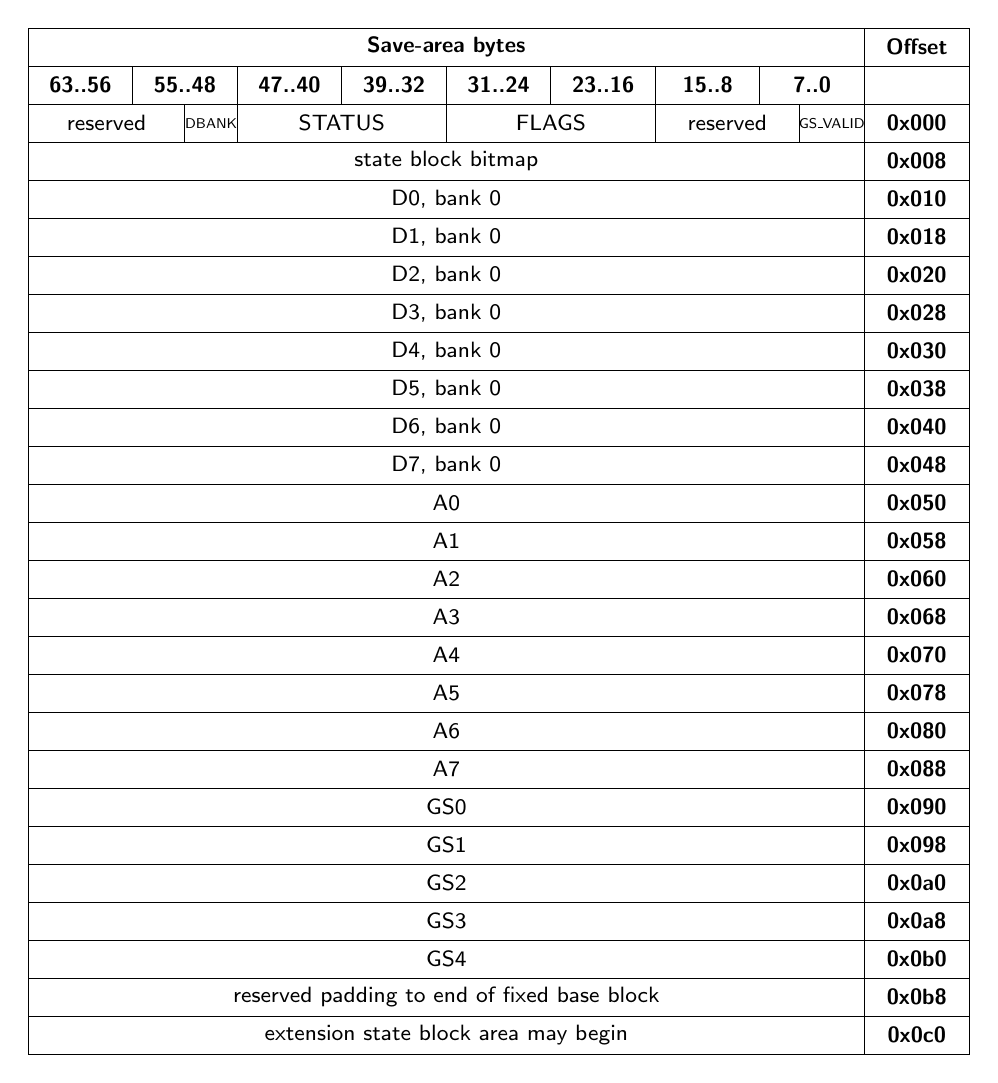
\begin{tikzpicture}[x=0.01368\linewidth,y=0.19in,every node/.style={font=\footnotesize,inner sep=1pt,align=center}]
\draw[line width=0.35pt] (0,0) rectangle (64,-1);
\node[font=\bfseries\footnotesize] at (32,-0.5) {Save-area bytes};
\draw[line width=0.35pt] (64,0) rectangle (72,-1);
\node[font=\bfseries\footnotesize] at (68,-0.5) {Offset};
\draw[line width=0.35pt] (0,-1) rectangle (8,-2);
\node[font=\bfseries\footnotesize] at (4,-1.5) {63..56};
\draw[line width=0.35pt] (8,-1) rectangle (16,-2);
\node[font=\bfseries\footnotesize] at (12,-1.5) {55..48};
\draw[line width=0.35pt] (16,-1) rectangle (24,-2);
\node[font=\bfseries\footnotesize] at (20,-1.5) {47..40};
\draw[line width=0.35pt] (24,-1) rectangle (32,-2);
\node[font=\bfseries\footnotesize] at (28,-1.5) {39..32};
\draw[line width=0.35pt] (32,-1) rectangle (40,-2);
\node[font=\bfseries\footnotesize] at (36,-1.5) {31..24};
\draw[line width=0.35pt] (40,-1) rectangle (48,-2);
\node[font=\bfseries\footnotesize] at (44,-1.5) {23..16};
\draw[line width=0.35pt] (48,-1) rectangle (56,-2);
\node[font=\bfseries\footnotesize] at (52,-1.5) {15..8};
\draw[line width=0.35pt] (56,-1) rectangle (64,-2);
\node[font=\bfseries\footnotesize] at (60,-1.5) {7..0};
\draw[line width=0.35pt] (64,-1) rectangle (72,-2);
\draw[line width=0.35pt] (0,-2) rectangle (12,-3);
\node at (6.00,-2.50) {reserved};
\draw[line width=0.35pt] (12,-2) rectangle (16,-3);
\node[scale=0.64] at (14.00,-2.50) {DBANK};
\draw[line width=0.35pt] (16,-2) rectangle (32,-3);
\node at (24.00,-2.50) {STATUS};
\draw[line width=0.35pt] (32,-2) rectangle (48,-3);
\node at (40.00,-2.50) {FLAGS};
\draw[line width=0.35pt] (48,-2) rectangle (59,-3);
\node at (53.50,-2.50) {reserved};
\draw[line width=0.35pt] (59,-2) rectangle (64,-3);
\node[scale=0.64] at (61.50,-2.50) {GS\_VALID};
\draw[line width=0.35pt] (64,-2) rectangle (72,-3);
\node[font=\bfseries\footnotesize] at (68,-2.50) {0x000};
\draw[line width=0.35pt] (0,-3) rectangle (64,-4);
\node at (32.00,-3.50) {state block bitmap};
\draw[line width=0.35pt] (64,-3) rectangle (72,-4);
\node[font=\bfseries\footnotesize] at (68,-3.50) {0x008};
\draw[line width=0.35pt] (0,-4) rectangle (64,-5);
\node at (32.00,-4.50) {D0, bank 0};
\draw[line width=0.35pt] (64,-4) rectangle (72,-5);
\node[font=\bfseries\footnotesize] at (68,-4.50) {0x010};
\draw[line width=0.35pt] (0,-5) rectangle (64,-6);
\node at (32.00,-5.50) {D1, bank 0};
\draw[line width=0.35pt] (64,-5) rectangle (72,-6);
\node[font=\bfseries\footnotesize] at (68,-5.50) {0x018};
\draw[line width=0.35pt] (0,-6) rectangle (64,-7);
\node at (32.00,-6.50) {D2, bank 0};
\draw[line width=0.35pt] (64,-6) rectangle (72,-7);
\node[font=\bfseries\footnotesize] at (68,-6.50) {0x020};
\draw[line width=0.35pt] (0,-7) rectangle (64,-8);
\node at (32.00,-7.50) {D3, bank 0};
\draw[line width=0.35pt] (64,-7) rectangle (72,-8);
\node[font=\bfseries\footnotesize] at (68,-7.50) {0x028};
\draw[line width=0.35pt] (0,-8) rectangle (64,-9);
\node at (32.00,-8.50) {D4, bank 0};
\draw[line width=0.35pt] (64,-8) rectangle (72,-9);
\node[font=\bfseries\footnotesize] at (68,-8.50) {0x030};
\draw[line width=0.35pt] (0,-9) rectangle (64,-10);
\node at (32.00,-9.50) {D5, bank 0};
\draw[line width=0.35pt] (64,-9) rectangle (72,-10);
\node[font=\bfseries\footnotesize] at (68,-9.50) {0x038};
\draw[line width=0.35pt] (0,-10) rectangle (64,-11);
\node at (32.00,-10.50) {D6, bank 0};
\draw[line width=0.35pt] (64,-10) rectangle (72,-11);
\node[font=\bfseries\footnotesize] at (68,-10.50) {0x040};
\draw[line width=0.35pt] (0,-11) rectangle (64,-12);
\node at (32.00,-11.50) {D7, bank 0};
\draw[line width=0.35pt] (64,-11) rectangle (72,-12);
\node[font=\bfseries\footnotesize] at (68,-11.50) {0x048};
\draw[line width=0.35pt] (0,-12) rectangle (64,-13);
\node at (32.00,-12.50) {A0};
\draw[line width=0.35pt] (64,-12) rectangle (72,-13);
\node[font=\bfseries\footnotesize] at (68,-12.50) {0x050};
\draw[line width=0.35pt] (0,-13) rectangle (64,-14);
\node at (32.00,-13.50) {A1};
\draw[line width=0.35pt] (64,-13) rectangle (72,-14);
\node[font=\bfseries\footnotesize] at (68,-13.50) {0x058};
\draw[line width=0.35pt] (0,-14) rectangle (64,-15);
\node at (32.00,-14.50) {A2};
\draw[line width=0.35pt] (64,-14) rectangle (72,-15);
\node[font=\bfseries\footnotesize] at (68,-14.50) {0x060};
\draw[line width=0.35pt] (0,-15) rectangle (64,-16);
\node at (32.00,-15.50) {A3};
\draw[line width=0.35pt] (64,-15) rectangle (72,-16);
\node[font=\bfseries\footnotesize] at (68,-15.50) {0x068};
\draw[line width=0.35pt] (0,-16) rectangle (64,-17);
\node at (32.00,-16.50) {A4};
\draw[line width=0.35pt] (64,-16) rectangle (72,-17);
\node[font=\bfseries\footnotesize] at (68,-16.50) {0x070};
\draw[line width=0.35pt] (0,-17) rectangle (64,-18);
\node at (32.00,-17.50) {A5};
\draw[line width=0.35pt] (64,-17) rectangle (72,-18);
\node[font=\bfseries\footnotesize] at (68,-17.50) {0x078};
\draw[line width=0.35pt] (0,-18) rectangle (64,-19);
\node at (32.00,-18.50) {A6};
\draw[line width=0.35pt] (64,-18) rectangle (72,-19);
\node[font=\bfseries\footnotesize] at (68,-18.50) {0x080};
\draw[line width=0.35pt] (0,-19) rectangle (64,-20);
\node at (32.00,-19.50) {A7};
\draw[line width=0.35pt] (64,-19) rectangle (72,-20);
\node[font=\bfseries\footnotesize] at (68,-19.50) {0x088};
\draw[line width=0.35pt] (0,-20) rectangle (64,-21);
\node at (32.00,-20.50) {GS0};
\draw[line width=0.35pt] (64,-20) rectangle (72,-21);
\node[font=\bfseries\footnotesize] at (68,-20.50) {0x090};
\draw[line width=0.35pt] (0,-21) rectangle (64,-22);
\node at (32.00,-21.50) {GS1};
\draw[line width=0.35pt] (64,-21) rectangle (72,-22);
\node[font=\bfseries\footnotesize] at (68,-21.50) {0x098};
\draw[line width=0.35pt] (0,-22) rectangle (64,-23);
\node at (32.00,-22.50) {GS2};
\draw[line width=0.35pt] (64,-22) rectangle (72,-23);
\node[font=\bfseries\footnotesize] at (68,-22.50) {0x0a0};
\draw[line width=0.35pt] (0,-23) rectangle (64,-24);
\node at (32.00,-23.50) {GS3};
\draw[line width=0.35pt] (64,-23) rectangle (72,-24);
\node[font=\bfseries\footnotesize] at (68,-23.50) {0x0a8};
\draw[line width=0.35pt] (0,-24) rectangle (64,-25);
\node at (32.00,-24.50) {GS4};
\draw[line width=0.35pt] (64,-24) rectangle (72,-25);
\node[font=\bfseries\footnotesize] at (68,-24.50) {0x0b0};
\draw[line width=0.35pt] (0,-25) rectangle (64,-26);
\node at (32.00,-25.50) {reserved padding to end of fixed base block};
\draw[line width=0.35pt] (64,-25) rectangle (72,-26);
\node[font=\bfseries\footnotesize] at (68,-25.50) {0x0b8};
\draw[line width=0.35pt] (0,-26) rectangle (64,-27);
\node at (32.00,-26.50) {extension state block area may begin};
\draw[line width=0.35pt] (64,-26) rectangle (72,-27);
\node[font=\bfseries\footnotesize] at (68,-26.50) {0x0c0};
\end{tikzpicture}\par\smallskip
\Needspace{2.40in}
\noindent\textbf{Base Header Fields:}\par\smallskip\noindent
\begingroup\footnotesize\renewcommand{\arraystretch}{1.08}
\begin{tabularx}{0.985\linewidth}{|p{0.56in}|p{0.62in}|p{1.35in}|X|}
\hline
\textbf{Offset} & \textbf{Bits} & \textbf{Field} & \textbf{Meaning}\\
\hline
0x000 & 0..4 & GS\_VALID & bit n validates GSn at 0x090 + 8*n; RESTORE updates only GS slots whose bits are set\\
\hline
0x000 & 5..15 & reserved & SAVE writes zero and RESTORE ignores\\
\hline
0x000 & 16..31 & FLAGS & always-saved integer condition-code FLAGS image\\
\hline
0x000 & 32..47 & STATUS & always-saved STATUS image; user-mode RESTORE ignores this field, supervisor RESTORE applies STATUS write rules\\
\hline
0x000 & 48..51 & DBANK & current data-register bank selector; RESTORE applies the SELDB validity rules and updates the selector after bank payloads\\
\hline
0x000 & 52..63 & reserved & SAVE writes zero and RESTORE ignores\\
\hline
0x008 & i & component descriptor 2+i present & i=0..SAVE\_COMPONENT\_COUNT-1 and SAVE\_COMPONENT\_COUNT must be no larger than 64\\
\hline
0x008 & all other bits & reserved & SAVE writes zero and RESTORE ignores\\
\hline
\end{tabularx}\endgroup\par\smallskip
\par\smallskip\noindent\textbf{Extension Component Formats:}\par
\par\smallskip\Needspace{2.4in}
\noindent\textbf{Extension Component: Additional Data-Register Banks}\par\smallskip
\begingroup\footnotesize
\begin{tabularx}{0.985\linewidth}{@{}p{1.35in}X@{}}
\textbf{Component ID} & 0x0001\\
\textbf{Component Name} & \texttt{DATA\_REGISTER\_BANKS}\\
\textbf{Component Size} & 0x40 * DBANK\_COUNT\\
\end{tabularx}\endgroup\par\smallskip
\Needspace{1.48in}
\noindent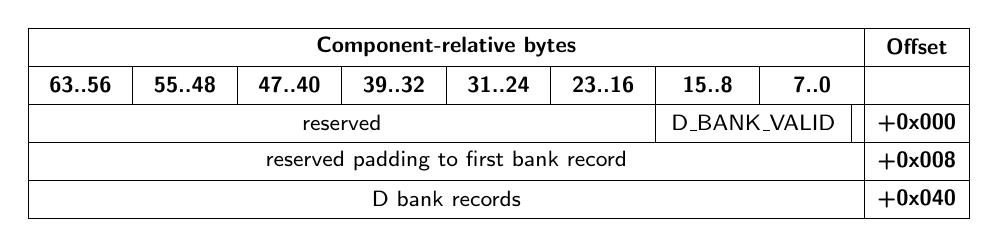
\begin{tikzpicture}[x=0.01368\linewidth,y=0.19in,every node/.style={font=\footnotesize,inner sep=1pt,align=center}]
\draw[line width=0.35pt] (0,0) rectangle (64,-1);
\node[font=\bfseries\footnotesize] at (32,-0.5) {Component-relative bytes};
\draw[line width=0.35pt] (64,0) rectangle (72,-1);
\node[font=\bfseries\footnotesize] at (68,-0.5) {Offset};
\draw[line width=0.35pt] (0,-1) rectangle (8,-2);
\node[font=\bfseries\footnotesize] at (4,-1.5) {63..56};
\draw[line width=0.35pt] (8,-1) rectangle (16,-2);
\node[font=\bfseries\footnotesize] at (12,-1.5) {55..48};
\draw[line width=0.35pt] (16,-1) rectangle (24,-2);
\node[font=\bfseries\footnotesize] at (20,-1.5) {47..40};
\draw[line width=0.35pt] (24,-1) rectangle (32,-2);
\node[font=\bfseries\footnotesize] at (28,-1.5) {39..32};
\draw[line width=0.35pt] (32,-1) rectangle (40,-2);
\node[font=\bfseries\footnotesize] at (36,-1.5) {31..24};
\draw[line width=0.35pt] (40,-1) rectangle (48,-2);
\node[font=\bfseries\footnotesize] at (44,-1.5) {23..16};
\draw[line width=0.35pt] (48,-1) rectangle (56,-2);
\node[font=\bfseries\footnotesize] at (52,-1.5) {15..8};
\draw[line width=0.35pt] (56,-1) rectangle (64,-2);
\node[font=\bfseries\footnotesize] at (60,-1.5) {7..0};
\draw[line width=0.35pt] (64,-1) rectangle (72,-2);
\draw[line width=0.35pt] (0,-2) rectangle (48,-3);
\node at (24.00,-2.50) {reserved};
\draw[line width=0.35pt] (48,-2) rectangle (63,-3);
\node at (55.50,-2.50) {D\_BANK\_VALID};
\draw[line width=0.35pt] (63,-2) rectangle (64,-3);
\draw[line width=0.35pt] (64,-2) rectangle (72,-3);
\node[font=\bfseries\footnotesize] at (68,-2.50) {+0x000};
\draw[line width=0.35pt] (0,-3) rectangle (64,-4);
\node at (32.00,-3.50) {reserved padding to first bank record};
\draw[line width=0.35pt] (64,-3) rectangle (72,-4);
\node[font=\bfseries\footnotesize] at (68,-3.50) {+0x008};
\draw[line width=0.35pt] (0,-4) rectangle (64,-5);
\node at (32.00,-4.50) {D bank records};
\draw[line width=0.35pt] (64,-4) rectangle (72,-5);
\node[font=\bfseries\footnotesize] at (68,-4.50) {+0x040};
\end{tikzpicture}\par\smallskip
\Needspace{1.27in}
\noindent\textbf{Component Header Fields:}\par\smallskip\noindent
\begingroup\footnotesize\renewcommand{\arraystretch}{1.08}
\begin{tabularx}{0.985\linewidth}{|p{0.56in}|p{0.62in}|p{1.35in}|X|}
\hline
\textbf{Offset} & \textbf{Bits} & \textbf{Field} & \textbf{Meaning}\\
\hline
+0x000 & 0 & reserved & bank 0 lives in the fixed base block\\
\hline
+0x000 & 1..15 & D\_BANK\_VALID & bit b validates D bank b at +0x040*b for b=1..DBANK\_COUNT-1\\
\hline
+0x000 & 16..63 & reserved & bits for unimplemented banks and future state are reserved\\
\hline
\end{tabularx}\endgroup\par\smallskip
\par\smallskip\Needspace{2.4in}
\noindent\textbf{Extension Component: Floating-Point State}\par\smallskip
\begingroup\footnotesize
\begin{tabularx}{0.985\linewidth}{@{}p{1.35in}X@{}}
\textbf{Component ID} & 0x0002\\
\textbf{Component Name} & \texttt{FLOATING\_POINT}\\
\textbf{Extension Requirement} & \texttt{floating\_point}\\
\textbf{Component Size} & 0x00c0\\
\end{tabularx}\endgroup\par\smallskip
\Needspace{4.48in}
\noindent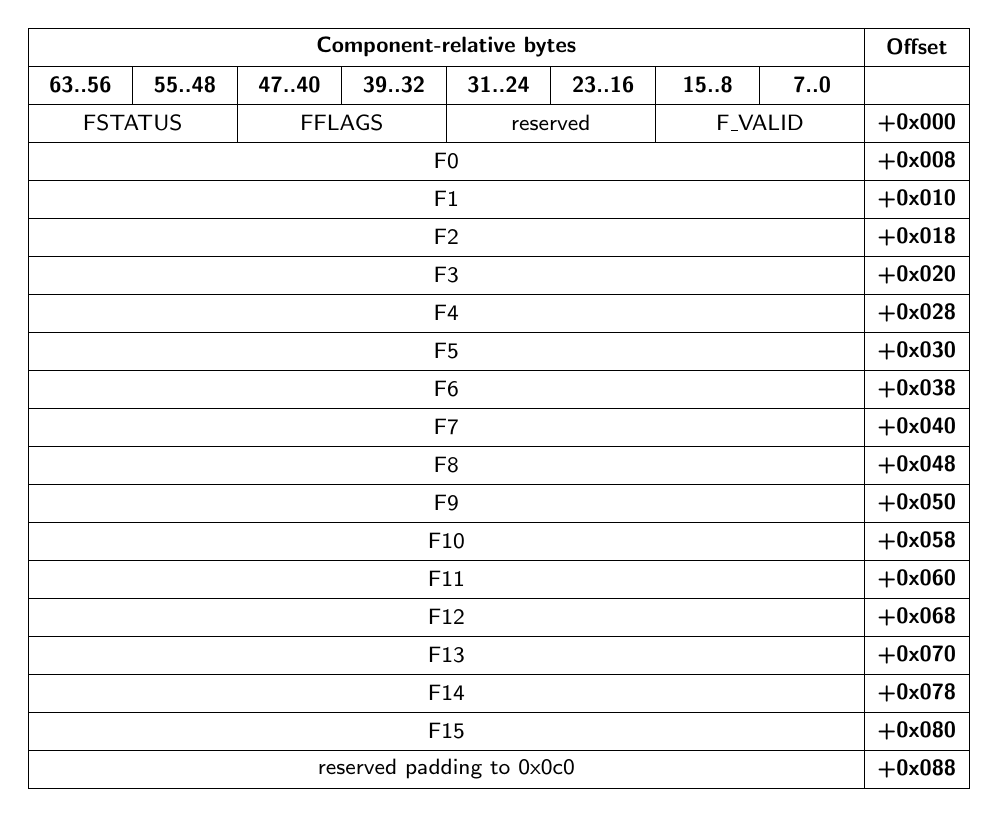
\begin{tikzpicture}[x=0.01368\linewidth,y=0.19in,every node/.style={font=\footnotesize,inner sep=1pt,align=center}]
\draw[line width=0.35pt] (0,0) rectangle (64,-1);
\node[font=\bfseries\footnotesize] at (32,-0.5) {Component-relative bytes};
\draw[line width=0.35pt] (64,0) rectangle (72,-1);
\node[font=\bfseries\footnotesize] at (68,-0.5) {Offset};
\draw[line width=0.35pt] (0,-1) rectangle (8,-2);
\node[font=\bfseries\footnotesize] at (4,-1.5) {63..56};
\draw[line width=0.35pt] (8,-1) rectangle (16,-2);
\node[font=\bfseries\footnotesize] at (12,-1.5) {55..48};
\draw[line width=0.35pt] (16,-1) rectangle (24,-2);
\node[font=\bfseries\footnotesize] at (20,-1.5) {47..40};
\draw[line width=0.35pt] (24,-1) rectangle (32,-2);
\node[font=\bfseries\footnotesize] at (28,-1.5) {39..32};
\draw[line width=0.35pt] (32,-1) rectangle (40,-2);
\node[font=\bfseries\footnotesize] at (36,-1.5) {31..24};
\draw[line width=0.35pt] (40,-1) rectangle (48,-2);
\node[font=\bfseries\footnotesize] at (44,-1.5) {23..16};
\draw[line width=0.35pt] (48,-1) rectangle (56,-2);
\node[font=\bfseries\footnotesize] at (52,-1.5) {15..8};
\draw[line width=0.35pt] (56,-1) rectangle (64,-2);
\node[font=\bfseries\footnotesize] at (60,-1.5) {7..0};
\draw[line width=0.35pt] (64,-1) rectangle (72,-2);
\draw[line width=0.35pt] (0,-2) rectangle (16,-3);
\node at (8.00,-2.50) {FSTATUS};
\draw[line width=0.35pt] (16,-2) rectangle (32,-3);
\node at (24.00,-2.50) {FFLAGS};
\draw[line width=0.35pt] (32,-2) rectangle (48,-3);
\node at (40.00,-2.50) {reserved};
\draw[line width=0.35pt] (48,-2) rectangle (64,-3);
\node at (56.00,-2.50) {F\_VALID};
\draw[line width=0.35pt] (64,-2) rectangle (72,-3);
\node[font=\bfseries\footnotesize] at (68,-2.50) {+0x000};
\draw[line width=0.35pt] (0,-3) rectangle (64,-4);
\node at (32.00,-3.50) {F0};
\draw[line width=0.35pt] (64,-3) rectangle (72,-4);
\node[font=\bfseries\footnotesize] at (68,-3.50) {+0x008};
\draw[line width=0.35pt] (0,-4) rectangle (64,-5);
\node at (32.00,-4.50) {F1};
\draw[line width=0.35pt] (64,-4) rectangle (72,-5);
\node[font=\bfseries\footnotesize] at (68,-4.50) {+0x010};
\draw[line width=0.35pt] (0,-5) rectangle (64,-6);
\node at (32.00,-5.50) {F2};
\draw[line width=0.35pt] (64,-5) rectangle (72,-6);
\node[font=\bfseries\footnotesize] at (68,-5.50) {+0x018};
\draw[line width=0.35pt] (0,-6) rectangle (64,-7);
\node at (32.00,-6.50) {F3};
\draw[line width=0.35pt] (64,-6) rectangle (72,-7);
\node[font=\bfseries\footnotesize] at (68,-6.50) {+0x020};
\draw[line width=0.35pt] (0,-7) rectangle (64,-8);
\node at (32.00,-7.50) {F4};
\draw[line width=0.35pt] (64,-7) rectangle (72,-8);
\node[font=\bfseries\footnotesize] at (68,-7.50) {+0x028};
\draw[line width=0.35pt] (0,-8) rectangle (64,-9);
\node at (32.00,-8.50) {F5};
\draw[line width=0.35pt] (64,-8) rectangle (72,-9);
\node[font=\bfseries\footnotesize] at (68,-8.50) {+0x030};
\draw[line width=0.35pt] (0,-9) rectangle (64,-10);
\node at (32.00,-9.50) {F6};
\draw[line width=0.35pt] (64,-9) rectangle (72,-10);
\node[font=\bfseries\footnotesize] at (68,-9.50) {+0x038};
\draw[line width=0.35pt] (0,-10) rectangle (64,-11);
\node at (32.00,-10.50) {F7};
\draw[line width=0.35pt] (64,-10) rectangle (72,-11);
\node[font=\bfseries\footnotesize] at (68,-10.50) {+0x040};
\draw[line width=0.35pt] (0,-11) rectangle (64,-12);
\node at (32.00,-11.50) {F8};
\draw[line width=0.35pt] (64,-11) rectangle (72,-12);
\node[font=\bfseries\footnotesize] at (68,-11.50) {+0x048};
\draw[line width=0.35pt] (0,-12) rectangle (64,-13);
\node at (32.00,-12.50) {F9};
\draw[line width=0.35pt] (64,-12) rectangle (72,-13);
\node[font=\bfseries\footnotesize] at (68,-12.50) {+0x050};
\draw[line width=0.35pt] (0,-13) rectangle (64,-14);
\node at (32.00,-13.50) {F10};
\draw[line width=0.35pt] (64,-13) rectangle (72,-14);
\node[font=\bfseries\footnotesize] at (68,-13.50) {+0x058};
\draw[line width=0.35pt] (0,-14) rectangle (64,-15);
\node at (32.00,-14.50) {F11};
\draw[line width=0.35pt] (64,-14) rectangle (72,-15);
\node[font=\bfseries\footnotesize] at (68,-14.50) {+0x060};
\draw[line width=0.35pt] (0,-15) rectangle (64,-16);
\node at (32.00,-15.50) {F12};
\draw[line width=0.35pt] (64,-15) rectangle (72,-16);
\node[font=\bfseries\footnotesize] at (68,-15.50) {+0x068};
\draw[line width=0.35pt] (0,-16) rectangle (64,-17);
\node at (32.00,-16.50) {F13};
\draw[line width=0.35pt] (64,-16) rectangle (72,-17);
\node[font=\bfseries\footnotesize] at (68,-16.50) {+0x070};
\draw[line width=0.35pt] (0,-17) rectangle (64,-18);
\node at (32.00,-17.50) {F14};
\draw[line width=0.35pt] (64,-17) rectangle (72,-18);
\node[font=\bfseries\footnotesize] at (68,-17.50) {+0x078};
\draw[line width=0.35pt] (0,-18) rectangle (64,-19);
\node at (32.00,-18.50) {F15};
\draw[line width=0.35pt] (64,-18) rectangle (72,-19);
\node[font=\bfseries\footnotesize] at (68,-18.50) {+0x080};
\draw[line width=0.35pt] (0,-19) rectangle (64,-20);
\node at (32.00,-19.50) {reserved padding to 0x0c0};
\draw[line width=0.35pt] (64,-19) rectangle (72,-20);
\node[font=\bfseries\footnotesize] at (68,-19.50) {+0x088};
\end{tikzpicture}\par\smallskip
\Needspace{1.51in}
\noindent\textbf{Component Header Fields:}\par\smallskip\noindent
\begingroup\footnotesize\renewcommand{\arraystretch}{1.08}
\begin{tabularx}{0.985\linewidth}{|p{0.56in}|p{0.62in}|p{1.35in}|X|}
\hline
\textbf{Offset} & \textbf{Bits} & \textbf{Field} & \textbf{Meaning}\\
\hline
+0x000 & 0..15 & F\_VALID & bit n validates Fn at +0x008 + 8*n\\
\hline
+0x000 & 16..31 & reserved & SAVE writes zero and RESTORE ignores\\
\hline
+0x000 & 32..47 & FFLAGS & floating-point accrued exception flags, always present when this state block is present\\
\hline
+0x000 & 48..63 & FSTATUS & floating-point control and status-mode register, always present when this state block is present\\
\hline
\end{tabularx}\endgroup\par\smallskip
\smallskip
\clearpage
\section{Data Formats}
\subsection{Integer Data Sizes}
Integer operands use four architectural sizes. The size suffix selects the number of low-order
bits used by the operation and the number of bytes transferred for memory operands.

\begingroup\footnotesize
\begin{longtable}{@{}p{0.75in}p{0.75in}p{0.75in}p{2.5in}@{}}
\toprule
\textbf{Suffix} & \textbf{Bits} & \textbf{Bytes} & \textbf{Name}\\
\midrule
\endhead
\texttt{B} & 8 & 1 & byte\\
\texttt{W} & 16 & 2 & word\\
\texttt{L} & 32 & 4 & long word\\
\texttt{Q} & 64 & 8 & quad word\\
\bottomrule
\end{longtable}
\manualtablecaption{Integer Data Sizes}
\endgroup

\begin{manuallistedformatdiagram}{Integer Register Operand Subfields}{4}
\manualformatrow{Q}{%
\manualformatfield{Q operand bits 63..0}{64}
}
\manualformatrow{L}{%
\manualformatfield{unchanged / instruction-defined}{32}
\manualformatfield{L operand bits 31..0}{32}
}
\manualformatrow{W}{%
\manualformatfield{unchanged / instruction-defined}{48}
\manualformatfield{W bits 15..0}{16}
}
\manualformatrow{B}{%
\manualformatfield{unchanged / instruction-defined}{56}
\manualformatfield{B bits 7..0}{8}
}
\end{manuallistedformatdiagram}

Byte, word, and long operations use the low-order subfield of the selected register. Q-sized
operations use the full 64-bit register. Instructions that explicitly extend a value define
whether the upper bits are sign-extended or zero-extended; otherwise, the instruction semantics
define whether upper bits are preserved, cleared, or replaced.

\subsection{Little-Endian Memory Organization}
Bedrock data memory is little-endian. For an N-byte integer value stored at byte address A, byte
A contains bits 7..0, byte A+1 contains bits 15..8, and so on. The least significant byte is
stored at the lowest address.

\begin{manuallistedbyteorderdiagram}{Little-Endian Byte Order for a 64-Bit Value}{byte}{address}{increasing addresses}{least significant byte first}{most significant byte last}
\manualbytecell{$V[7..0]$}{A+0}
\manualbytecell{$V[15..8]$}{A+1}
\manualbytecell{$V[23..16]$}{A+2}
\manualbytecell{$V[31..24]$}{A+3}
\manualbytecell{$V[39..32]$}{A+4}
\manualbytecell{$V[47..40]$}{A+5}
\manualbytecell{$V[55..48]$}{A+6}
\manualbytecell{$V[63..56]$}{A+7}
\end{manuallistedbyteorderdiagram}

\[
\mathit{mem}[A+i] = (\mathit{value} \gg (8i)) \mathbin{\&} 255,\qquad 0 \le i < N
\]

The same byte order is used for instruction words, immediate payloads, displacement payloads,
absolute-address payloads, and data transferred by load/store instructions.

\begin{manuallistedbyteorderdiagram}{Instruction Word Storage in Memory}{instruction word}{}{instruction stream byte order}{}{}
\manualbytecell{$word[7:0]$}{PC+0}
\manualbytecell{$word[15:8]$}{PC+1}
\end{manuallistedbyteorderdiagram}

\subsection{Instruction Payload Ordering}
Instruction length is measured in 16-bit words, but each instruction word is itself stored in
little-endian byte order. Word 0 occupies the first two bytes of the instruction. If a prefix
word, descriptor word, immediate, displacement, or bitmap follows, those words occupy increasing
addresses in decode order.

\begingroup\footnotesize
\begin{longtable}{@{}p{0.85in}p{0.85in}p{3.8in}@{}}
\toprule
\textbf{Payload} & \textbf{Words} & \textbf{Memory Order}\\
\midrule
\endhead
\texttt{imm16} & 1 word & bits 7..0 at the lower byte, bits 15..8 at the next byte\\
\texttt{imm32} & 2 words & least significant word first, then most significant word\\
\texttt{imm64} & 4 words & least significant word first through most significant word\\
\texttt{disp16} & 1 word & signed two's-complement value\\
\texttt{disp32} & 2 words & signed two's-complement value, least significant word first\\
\texttt{disp64} & 4 words & signed two's-complement value, least significant word first\\
\bottomrule
\end{longtable}
\manualtablecaption{Immediate and Displacement Payload Order}
\endgroup

Multiword immediates and displacements are stored least significant word first. Signed displacement
payloads use two's-complement representation at their declared width before any sign extension
performed by the consuming instruction or effective-address form.

When an instruction operand has an explicit operation size and encodes an immediate operand narrower
than that operation size, the operand kind defines how the encoded value is extended before use.
Immediate operands on forms without an operation size are interpreted by that instruction form rather
than by this operation-size rule.

\begin{manuallongtable}{@{}>{\raggedright\arraybackslash}p{0.70in}>{\raggedright\arraybackslash}p{0.45in}>{\raggedright\arraybackslash}p{0.70in}>{\raggedright\arraybackslash}p{0.75in}>{\raggedright\arraybackslash}p{1.55in}>{\raggedright\arraybackslash}p{1.35in}@{}}
\toprule
\textbf{Operand} & \textbf{Bits} & \textbf{Value} & \textbf{Range} & \textbf{Operation-Size Rule} & \textbf{Applies When}\\
\midrule
\endhead
\texttt{imm6} & 6 & unsigned & 0..63 & zero-extend to the operation size & integer forms with an explicit B/W/L/Q operation size\\
\bottomrule
\end{manuallongtable}
\manualtablecaption{Immediate Operand Interpretation}


\subsection{Floating-Point Data Formats}
Floating-point scalar formats are little-endian in memory as well. The S format is 32 bits and the
D format is 64 bits. The bit-level floating-point encoding, NaN policy, exception flags, and
rounding behavior are described by the floating-point programming model and instruction metadata;
their memory byte order follows the same least-significant-byte-first rule as integer data.

\clearpage
\section{Condition Codes}
Conditional instructions encode a four-bit condition code. The zero-valued condition is T, which is also
used for canonical aliases such as JMP for Jcc.T and TRAP for TRAPcc.T. The condition-code bits are the
low four meaningful bits of FLAGS, as shown in the Register Model section.

\begin{manuallongtable}{@{}>{\raggedright\arraybackslash}p{0.65in}>{\raggedright\arraybackslash}p{0.65in}>{\raggedright\arraybackslash}p{1.05in}>{\raggedright\arraybackslash}p{2.95in}@{}}
\toprule
\textbf{Code} & \textbf{Value} & \textbf{Aliases} & \textbf{Expression}\\
\midrule
\endhead
\texttt{T} & \texttt{0x0} & - & \texttt{true}\\
\texttt{F} & \texttt{0x1} & - & \texttt{false}\\
\texttt{EQ} & \texttt{0x2} & Z & \texttt{Z == 1}\\
\texttt{NE} & \texttt{0x3} & NZ & \texttt{Z == 0}\\
\texttt{ULT} & \texttt{0x4} & C & \texttt{C == 1}\\
\texttt{UGE} & \texttt{0x5} & NC & \texttt{C == 0}\\
\texttt{MI} & \texttt{0x6} & N & \texttt{N == 1}\\
\texttt{PL} & \texttt{0x7} & NN & \texttt{N == 0}\\
\texttt{VS} & \texttt{0x8} & V & \texttt{V == 1}\\
\texttt{VC} & \texttt{0x9} & NV & \texttt{V == 0}\\
\texttt{ULE} & \texttt{0xa} & - & \texttt{C == 1 \textbar{}\textbar{} Z == 1}\\
\texttt{UGT} & \texttt{0xb} & - & \texttt{C == 0 \&\& Z == 0}\\
\texttt{LT} & \texttt{0xc} & - & \texttt{N != V}\\
\texttt{GE} & \texttt{0xd} & - & \texttt{N == V}\\
\texttt{LE} & \texttt{0xe} & - & \texttt{Z == 1 \textbar{}\textbar{} N != V}\\
\texttt{GT} & \texttt{0xf} & - & \texttt{Z == 0 \&\& N == V}\\
\bottomrule
\end{manuallongtable}
\manualtablecaption{Condition Codes}


\clearpage
\section{Prefixes}
Prefix words modify the following instruction. One prefix word contains two 8-bit slots; the low byte is filled
and decoded first, and the high byte is filled and decoded second. The table below lists standalone prefix
spellings and assembler-generated repeat-boundary bytes. Address-update and user-access forms are shown
separately because they are selected by operand syntax.

\begin{manuallongtable}{@{}>{\raggedright\arraybackslash}p{1.45in}>{\raggedright\arraybackslash}p{0.95in}>{\raggedright\arraybackslash}p{3.0in}@{}}
\toprule
\textbf{Syntax} & \textbf{Byte/Pattern} & \textbf{Meaning}\\
\midrule
\endhead
\texttt{NPX} & \texttt{0x00} & no effect\\
\texttt{NOSPEC} & \texttt{0x01} & speculation boundary\\
\texttt{SAT} & \texttt{0x02} & saturating arithmetic\\
\texttt{NT} & \texttt{0x03} & non-temporal memory hint\\
\texttt{REP\{cc\} Dn, instr} & \texttt{1ccc cddd} & repeat while counter and condition remain active\\
\texttt{REPG Dn, \{...\}} & \texttt{0111 0ddd} & repeat grouped instructions using the selected counter\\
\texttt{ENDG} & \texttt{0x78} & end grouped repeat\\
\bottomrule
\end{manuallongtable}
\manualtablecaption{Prefix Encodings}


\subsection{Address-Update Operand Syntax}
Address update is selected by the memory operand spelling, not by a standalone prefix mnemonic. The assembler
emits the corresponding prefix byte only for update-eligible indirect EA forms. Because legality depends on the
selected EA form, address update is not listed as a separate per-mnemonic column in the instruction attribute
matrix.

\begin{manuallongtable}{@{}>{\raggedright\arraybackslash}p{1.25in}>{\raggedright\arraybackslash}p{0.75in}>{\raggedright\arraybackslash}p{3.1in}@{}}
\toprule
\textbf{Operand Syntax} & \textbf{Byte} & \textbf{Update}\\
\midrule
\endhead
\texttt{[An++]} & \texttt{0x04} & Address-update prefix for update-eligible indirect EA forms; the address register is incremented after the access.\\
\texttt{[++An]} & \texttt{0x05} & Address-update prefix for update-eligible indirect EA forms; the address register is incremented before the access.\\
\texttt{[An{-}{-}]} & \texttt{0x06} & Address-update prefix for update-eligible indirect EA forms; the address register is decremented after the access.\\
\texttt{[{-}{-}An]} & \texttt{0x07} & Address-update prefix for update-eligible indirect EA forms; the address register is decremented before the access.\\
\bottomrule
\end{manuallongtable}
\manualtablecaption{Address-Update Encodings}



\subsection{User Access Operand Syntax}
Memory operands use the current-domain \texttt{C} by default. Assembly source may annotate memory operands
with \texttt{U:} to request a user-domain access. The assembler maps the annotated source and destination
domains to one encoded access-domain prefix. Explicit \texttt{C:} is allowed for readability but is
usually omitted. Operand positions that are not memory accesses do not contribute to prefix selection. If no
user-domain memory access is present, no access-domain prefix is needed.

\begin{manuallongtable}{@{}>{\raggedright\arraybackslash}p{1.65in}>{\raggedright\arraybackslash}p{0.75in}>{\raggedright\arraybackslash}p{3.0in}@{}}
\toprule
\textbf{Operand Domains} & \textbf{Byte} & \textbf{Encoded Meaning}\\
\midrule
\endhead
\texttt{U:[src], C:[dst]} & \texttt{0x08} & user-domain source to current-domain destination\\
\texttt{C:[src], U:[dst]} & \texttt{0x09} & current-domain source to user-domain destination\\
\texttt{U:[src], U:[dst]} & \texttt{0x0a} & user-domain memory operands\\
\bottomrule
\end{manuallongtable}
\manualtablecaption{User-Access Operand Encodings}



\subsection{Prefix Semantics}
Prefix bytes are interpreted as modifiers of the immediately following instruction only. Assemblers should
avoid redundant or contradictory prefixes, but architectural prefix interpretation remains deterministic
because later prefix slots override earlier conflicting effects.

\Needspace{0.75in}\manualfield{\texttt{NPX}:}{Neutral prefix byte and canonical filler for an unused prefix slot.}
\Needspace{0.75in}\manualfield{\texttt{NOSPEC}:}{Marks the following instruction as a speculation boundary or speculation-limited operation.}
\Needspace{0.75in}\manualfield{\texttt{SATURATE}:}{Requests the saturating form of arithmetic instructions that define one.\newline Applies to: arithmetic}
\Needspace{0.75in}\manualfield{\texttt{NONTEMPORAL}:}{Provides a cache-allocation hint for memory operations without changing the architectural loaded or stored value.\newline Applies to: memory}
\Needspace{0.75in}\manualfield{\texttt{U2C}:}{Access-domain prefix selected by the U:[src], C:[dst] operand annotation.\newline Applies to: memory\newline Examples: \texttt{MOV.Q U:[A0], D0}, \texttt{MOV.B U:[A0++], C:[A1++]}}
\Needspace{0.75in}\manualfield{\texttt{C2U}:}{Access-domain prefix selected by the C:[src], U:[dst] operand annotation.\newline Applies to: memory\newline Examples: \texttt{MOV.Q D0, U:[A1]}, \texttt{MOV.B C:[A0++], U:[A1++]}}
\Needspace{0.75in}\manualfield{\texttt{U2U}:}{Access-domain prefix selected by the U:[src], U:[dst] operand annotation.\newline Applies to: memory\newline Examples: \texttt{MOV.B U:[A0++], U:[A1++]}, \texttt{INC.L U:[A0]}}


\subsection{Conditional Repeat Prefix REPcc}
REPcc is the conditional repeat prefix family. It combines a D-register repeat counter with a full
condition-code selector, then applies that repeat contract to the following instruction. REP is the
canonical alias for REPT.

The selected D register remains an ordinary signed two's-complement value. REP/REPcc tests that value for zero
before each iteration. After the instruction body completes, REPFLAGS are computed from the observed value; the
counter moves one step toward zero only when the selected REP condition remains true. A completed terminating
iteration whose REP condition is false commits the instruction body's ordinary side effects but leaves the
counter unchanged. If the same D register appears in an indexed effective address, EA evaluation uses the same
architectural value before the iteration update.

\begin{manuallongtable}{@{}>{\raggedright\arraybackslash}p{1.35in}>{\raggedright\arraybackslash}p{4.1in}@{}}
\toprule
\textbf{Item} & \textbf{Value}\\
\midrule
\endhead
Syntax & \texttt{REPcc Dn, \textless{}instruction\textgreater{}}\\
Alias & REP = REPT\\
FPU conditional subset & \begin{tabular}[t]{@{}l@{}}FCMP\\FTEST\\FBNDII\\FBNDIX\\FBNDXI\\FBNDXX\end{tabular}\\
FPU status predicates & not supported\\
Counter & DREG, signed counter moves toward zero\\
Counter encoding & signed two's-complement; bits 63..0\\
Zero test & zero counter performs no iteration\\
REP index value & architectural counter value before iteration update\\
Condition-true update & positive counters decrement and negative counters increment toward zero\\
Condition-false update & counter is not updated\\
Commit rule & a condition-false terminating iteration commits the body and leaves the counter unchanged\\
Condition source & REPFLAGS from the iteration observed value\\
Architectural flags & body instruction rules apply to the last completed iteration\\
FFLAGS & bitwise inclusive-or of completed iterations\\
\bottomrule
\end{manuallongtable}
\manualtablecaption{REPcc Prefix Rules}


Repeats the following instruction using the selected D-register counter and condition-code selector.

\begin{manuallongtable}{@{}>{\raggedright\arraybackslash}p{0.85in}>{\raggedright\arraybackslash}p{1.95in}>{\raggedright\arraybackslash}p{2.65in}@{}}
\toprule
\textbf{Mnemonic} & \textbf{Observed Value} & \textbf{REPFLAGS Rule}\\
\midrule
\endhead
\texttt{CMP} & right operand minus left operand & compute subtract flags from right operand minus left operand\\
\texttt{EXTSL} & result value & set Z/N from observed value and clear C/V\\
\texttt{EXTSQ} & result value & set Z/N from observed value and clear C/V\\
\texttt{EXTSW} & result value & set Z/N from observed value and clear C/V\\
\texttt{EXTZL} & result value & set Z/N from observed value and clear C/V\\
\texttt{EXTZQ} & result value & set Z/N from observed value and clear C/V\\
\texttt{EXTZW} & result value & set Z/N from observed value and clear C/V\\
\texttt{FBNDII} & - & set V from interval check\\
\texttt{FBNDIX} & - & set V from interval check\\
\texttt{FBNDXI} & - & set V from interval check\\
\texttt{FBNDXX} & - & set V from interval check\\
\texttt{FCMP} & - & floating-point compare flag rules\\
\texttt{FTEST} & - & floating-point compare flag rules\\
\texttt{MOV} & source value & set Z/N from observed value and clear C/V\\
\texttt{TEST} & left operand bitwise-and right operand & set Z/N from observed value and clear C/V\\
\bottomrule
\end{manuallongtable}
\manualtablecaption{REPcc Observed Values}


\paragraph{REPcc Operation Examples.}
The following examples show how the observed value, REPFLAGS, counter update,
and terminating iteration interact for common operation classes. In each case,
the counter is tested before the body executes. The body then computes an
observed value, derives REPFLAGS from that value, and updates the counter only
when the selected REP condition remains true.

\paragraph{Counted Move.}
Plain REP is the REPT alias, so the condition is always true. This form copies
exactly the requested count, and the counter reaches zero when the transfer
finishes.

\begin{quote}
\begingroup\small\ttfamily
\begin{tabular}{@{}l@{}}
; D0 = -n, A0 = src + n, A1 = dst + n\\
REP D0, MOV.B [A0 + D0 * 1], [A1 + D0 * 1]\\
\end{tabular}
\endgroup
\end{quote}

For MOV, the observed value is the source value. REPT does not use it to stop;
the body commits and the counter moves toward zero after every completed
iteration.

\paragraph{Scan Until Zero.}
MOV can also be used with REPNE to scan a stream while the loaded value remains
nonzero.

\begin{quote}
\begingroup\small\ttfamily
\begin{tabular}{@{}l@{}}
; D0 = n, A0 = base\\
MOV.L D0, D1\\
REPNE D1, MOV.L [A0++], D2\\
SUB.L D1, D0\\
\end{tabular}
\endgroup
\end{quote}

The MOV body loads the candidate element into D2 and uses that loaded value as
the observed value. If the value is nonzero, REPNE is true and D1 is decremented.
If the value is zero, the load and address update still commit, but D1 is not
decremented. The final subtraction therefore produces the zero element index
without a separate off-by-one correction.

\paragraph{Compare While Equal.}
CMP uses the subtraction result as the observed value. REPEQ continues while the
comparison is equal and stops on the first non-equal comparison or when the
counter reaches zero.

\begin{quote}
\begingroup\small\ttfamily
\begin{tabular}{@{}l@{}}
; D0 = -n, A0 = a + n, A1 = b + n\\
REPEQ D0, CMP.B [A0 + D0 * 1], [A1 + D0 * 1]\\
\end{tabular}
\endgroup
\end{quote}

When a mismatch is found, the terminating CMP commits its FLAGS result and the
counter is not updated for that terminating iteration. Software can use the final
FLAGS state to derive the ordered result.

\paragraph{Test While Nonzero.}
TEST derives REPFLAGS from the logical test result. A memory scan can therefore
continue while a masked value remains nonzero, or stop when a selected bit range
clears.

\begin{quote}
\begingroup\small\ttfamily
\begin{tabular}{@{}l@{}}
; D0 = n, A0 = base, D3 = mask\\
REPNE D0, TEST.L [A0++], D3\\
\end{tabular}
\endgroup
\end{quote}

The memory operand and mask are tested each iteration. A nonzero tested result
updates the counter and continues; a zero tested result commits the TEST FLAGS
and leaves the counter at the terminating element.

\paragraph{Bulk Extension.}
The EXTS and EXTZ memory forms use the widened result as the observed value. An
unconditional REP form expresses a compact bulk conversion, while a conditional
form can stop when a converted value matches the selected condition.

\begin{quote}
\begingroup\small\ttfamily
\begin{tabular}{@{}l@{}}
; D0 = n, A0 = byte source, A1 = long destination\\
REP D0, EXTZL.B [A0++], [A1++]\\
\end{tabular}
\endgroup
\end{quote}

The source byte is read, zero-extended to a long value, and written to the
destination element. Because REP is REPT, every completed conversion updates the
counter.


\subsection{Grouped Repeat Prefix REPG}
REPG repeats an ENDG-terminated block of instructions with a D-register
counter. The first grouped instruction carries the REPG prefix byte; the final
grouped instruction carries the ENDG prefix byte. Instructions between those
endpoints are ordinary instruction records with their own word 0 length fields.
The grouped instructions execute in program order and have no condition-code
selector.

Architecturally, REPG is a compact spelling for a counted scalar loop over a
short straight-line instruction trace. One group iteration executes every
instruction from the REPG-marked instruction through the ENDG-marked instruction
exactly once, in instruction-stream order. After a successful group iteration,
the selected D register is moved one step toward zero. A zero counter performs
no group iteration. Positive counters count down; negative counters count up
toward zero.

\paragraph{Group Discovery.}
A REPG group is discovered entirely from the architectural instruction stream.
When a REPG prefix is seen, instruction interpretation follows the explicit word
0 length fields of subsequent instruction records in the same naturally aligned
64-byte grouping window until it reaches an instruction carrying ENDG. ENDG may
appear on the same instruction as REPG, which forms a one-instruction group. A
well-formed REPG group has exactly one active REPG start marker, exactly one ENDG
terminator, and no nested repeat prefix inside the group.

\paragraph{Fast-Contract Source Form.}
\texttt{REPGF} is a source-level assertion that uses the same architectural
encoding as \texttt{REPG}. It does not allocate a second prefix byte and does
not force a particular implementation strategy. It marks the group as a
REPG-fast candidate: the selected counter register is outside the group writes,
the effective addresses are regular, and the group avoids control, state, and
nested-repeat operations. Runtime properties such as ordinary mapped memory
remain architectural preconditions of the fast class rather than extra encoded
bits.

\paragraph{Grouping Window.}
The complete byte range occupied by the grouped instructions must fit within the
naturally aligned 64-byte grouping window that contains the first grouped
instruction. The first instruction does not need to be aligned to the beginning
of the window; only containment matters. This keeps architectural group
recognition bounded while avoiding any dependency on a particular
implementation's instruction-fetch granularity.

\paragraph{Execution and Faults.}
Each grouped instruction retains its ordinary operand decoding,
effective-address calculation, privilege checks, FLAGS or FFLAGS behavior, and
memory side effects. Address-update operands update as they would in scalar
execution for each completed instruction.

If a fault occurs, completed iterations and completed instructions in the
current iteration remain committed, and the fault is precise at the faulting
grouped instruction. The counter update for an iteration occurs only after the
whole group iteration completes successfully. A REPG fault frame saves the PC of
the faulting grouped instruction and a compact repeat continuation in
\texttt{FAULT\_AUX}. The group start is not stored as a full address; it is
reconstructed from a five-bit unsigned negative word displacement:

\[
  \texttt{group\_start\_pc}
  =
  \texttt{fault\_pc}
  -
  2 \times \texttt{group\_start\_delta\_words}
\]

The group index is not saved. If the handler returns without editing the frame,
IRET resumes at the saved PC under the active REPG continuation and then
proceeds through the rest of the group.

\paragraph{Group Model.}
A REPG group is intended to be straight-line code. Branches, calls, returns,
traps, system-call returns, interrupt returns, atomics, stack operations,
nested repeat prefixes, and state-mutating system, TLB, cache, or fence
operations are outside the REPG group model.

REPG optimization is divided into REPG-fast and REPG-general. REPG-fast
identifies groups that are suitable for internal SIMD or streaming recognition.
REPG-general preserves exact scalar semantics for less regular groups, including
groups with selected-counter dependencies.

\begingroup\small
\begin{longtable}{@{}p{1.35in}p{4.45in}@{}}
\toprule
\textbf{Item} & \textbf{Value}\\
\midrule
Syntax & source uses \texttt{REPG Dn,} followed by a braced instruction list\\
Fast-contract syntax & source may use \texttt{REPGF Dn,} followed by a braced instruction list; the emitted encoding is the same as \texttt{REPG}\\
Condition selector & none\\
Counter & D register\\
Group termination & ENDG prefix on the final grouped instruction\\
Fast-contract marker & REPG-fast candidate when the group satisfies the fast rules\\
Grouping window & grouped instruction bytes must fit in one naturally aligned 64-byte window\\
Commit rule & completed iterations and completed prior group instructions commit\\
Fault continuation & saved PC is the faulting grouped instruction; group-start delta is a 5-bit negative word displacement; no group index is saved\\
FFLAGS & OR of completed iterations\\
\bottomrule
\end{longtable}
\manualtablecaption{REPG Prefix Rules}
\endgroup

\begingroup\small
\begin{longtable}{@{}p{0.95in}p{2.15in}p{2.55in}@{}}
\toprule
\textbf{Class} & \textbf{Availability} & \textbf{Implementation}\\
\midrule
\texttt{REPG-fast} &
\begin{tabular}[t]{@{}l@{}}
counter Dn is not written\\
regular effective addresses\\
ordinary memory\\
no control or state changes
\end{tabular}
& internal SIMD or streaming optimization is possible\\
\texttt{REPG-general} &
\begin{tabular}[t]{@{}l@{}}
counter Dn may be read or written\\
state-query instructions may appear\\
wait-like instructions may appear\\
examples: WAIT, CPUID
\end{tabular}
& exact scalar semantics, with no fast streaming guarantee\\
\bottomrule
\end{longtable}
\manualtablecaption{REPG Optimization Classes}
\endgroup

\paragraph{Example.}
\begin{quote}
\begingroup\small\ttfamily
\begin{tabular}{@{}l@{}}
REPG D2, \{\\
\quad MOV.L  [A1++], D4\\
\quad MADD.L [A0++], D4, D1\\
\}\\
\end{tabular}
\endgroup
\end{quote}

The example repeats a two-instruction dot-product step. Each iteration loads one
source value, performs one multiply-add using the other source stream, advances
the update-eligible addresses, and then updates D2 toward zero after the whole
group completes.


\clearpage
\section{Effective Addressing Modes}
Effective-address operands are encoded through a compact six-bit EA field. Most instructions that accept EA
therefore share the same operand sublayout, which keeps register and memory forms visually regular. The high
three bits select the addressing family and the low three bits normally carry the register number or a small
form selector. Forms that need displacement, absolute address, immediate data, or an extended descriptor append
payload words after the instruction word.

\begin{manuallistedformatdiagram}{Compact Effective-Address Field}{1}
\manualformatrow{EA[5:0]}{%
\manualformatfield{mode}{3}
\manualformatfield{register/form}{3}
}
\end{manuallistedformatdiagram}


\begin{manuallistedformatdiagram}{Compact EA Form Map}{1}
\manualformatrow{DREG}{%
\manualformatfieldcode{000}{3}
\manualformatfieldcode{d}{3}
}
\manualformatrow{AREG}{%
\manualformatfieldcode{001}{3}
\manualformatfieldcode{a}{3}
}
\manualformatrow{[A]}{%
\manualformatfieldcode{010}{3}
\manualformatfieldcode{a}{3}
}
\manualformatrow{[A + disp16]}{%
\manualformatfieldcode{011}{3}
\manualformatfieldcode{a}{3}
}
\manualformatrow{[A + disp32]}{%
\manualformatfieldcode{100}{3}
\manualformatfieldcode{a}{3}
}
\manualformatrow{PC/SP}{%
\manualformatfieldcode{101}{3}
\manualformatfieldcode{x}{3}
}
\manualformatrow{ABS/IMM}{%
\manualformatfieldcode{110}{3}
\manualformatfieldcode{x}{3}
}
\manualformatrow{S32 XEA}{%
\manualformatfieldcode{1111}{4}
\manualformatfieldcode{10}{2}
}
\manualformatrow{XEA}{%
\manualformatfieldcode{1111}{4}
\manualformatfieldcode{11}{2}
}
\end{manuallistedformatdiagram}


Compact EA forms keep the register selector in EA[2:0] whenever the form is register-based. The PC/SP, absolute,
and immediate groups reuse those low bits as form selectors. The S32 XEA and XEA compact forms are escapes to
the descriptor shown below.

\begin{manuallistedformatdiagram}{Compact EA Payload Sequence}{1}
\manualformatrow{EA field}{%
\manualformatfieldcode{m}{4}
\manualformatfieldcode{r}{2}
}
\manualformatrow{optional word 1}{%
\manualformatfieldcode{p}{16}
}
\manualformatrow{optional word 2}{%
\manualformatfieldcode{p}{16}
}
\end{manuallistedformatdiagram}


\subsection{Compact EA Addressing Modes}
\Needspace{3.9in}
\par\smallskip\noindent{\bfseries Data Register Direct}\par
Direct data-register operand. The EA field selects Dn and does not imply a memory access.
\manualfield{Generation:}{operand = contents(Dn)}
\manualfield{Assembler Syntax:}{\texttt{Dn}}
\manualfield{Encoding:}{\texttt{000 ddd}}
\manualfield{Payload:}{no payload words}
\manualfield{Address Update:}{not eligible}
\manualeadirectflow{Direct operand selection for Data Register Direct}{DATA REGISTER}{Dn CONTENTS}{REGISTER VALUE}

\Needspace{3.9in}
\par\smallskip\noindent{\bfseries Address Register Direct}\par
Direct address-register operand. The EA field selects An and does not imply a memory access.
\manualfield{Generation:}{operand = contents(An)}
\manualfield{Assembler Syntax:}{\texttt{An}}
\manualfield{Encoding:}{\texttt{001 aaa}}
\manualfield{Payload:}{no payload words}
\manualfield{Address Update:}{not eligible}
\manualeadirectflow{Direct operand selection for Address Register Direct}{ADDRESS REGISTER}{An CONTENTS}{REGISTER VALUE}

\Needspace{4.5in}
\par\smallskip\noindent{\bfseries Address Register Indirect}\par
address-register indirect memory operand. address-update prefixes may use this form.
\manualfield{Generation:}{EA = contents(An)}
\manualfield{Assembler Syntax:}{\texttt{[A]}}
\manualfield{Encoding:}{\texttt{010 aaa}}
\manualfield{Payload:}{no payload words}
\manualfield{Address Update:}{eligible}
\manualeasimplememoryflow{Address calculation for Address Register Indirect}{ADDRESS REGISTER}{An CONTENTS}{EFFECTIVE ADDRESS}

\Needspace{4.7in}
\par\smallskip\noindent{\bfseries Address Register Indirect with disp16}\par
address-register relative memory operand. with a signed 16-bit displacement payload.
\manualfield{Generation:}{EA = contents(An) + disp16}
\manualfield{Assembler Syntax:}{\texttt{[A + disp16]}}
\manualfield{Encoding:}{\texttt{011 aaa}}
\manualfield{Payload:}{one signed 16-bit displacement word}
\manualfield{Address Update:}{not eligible}
\manualeaadditivememoryflow{Address calculation for Address Register Indirect with disp16}{ADDRESS REGISTER}{An CONTENTS}{SIGN-EXTENDED disp16}{EFFECTIVE ADDRESS}

\Needspace{4.7in}
\par\smallskip\noindent{\bfseries Address Register Indirect with disp32}\par
address-register relative memory operand. with a signed 32-bit displacement payload.
\manualfield{Generation:}{EA = contents(An) + disp32}
\manualfield{Assembler Syntax:}{\texttt{[A + disp32]}}
\manualfield{Encoding:}{\texttt{100 aaa}}
\manualfield{Payload:}{two signed 32-bit displacement words}
\manualfield{Address Update:}{not eligible}
\manualeaadditivememoryflow{Address calculation for Address Register Indirect with disp32}{ADDRESS REGISTER}{An CONTENTS}{SIGN-EXTENDED disp32}{EFFECTIVE ADDRESS}

\Needspace{4.7in}
\par\smallskip\noindent{\bfseries Program Counter Relative with disp16}\par
program-counter relative memory operand. with a signed 16-bit displacement payload. using fixed CS segment selection.
\manualfield{Generation:}{EA = PC + disp16}
\manualfield{Assembler Syntax:}{\texttt{[PC + disp16]}}
\manualfield{Encoding:}{\texttt{101000}}
\manualfield{Payload:}{one signed 16-bit displacement word}
\manualfield{Address Update:}{not eligible}
\manualeaadditivememoryflow{Address calculation for Program Counter Relative with disp16}{PROGRAM COUNTER}{PC}{SIGN-EXTENDED disp16}{EFFECTIVE ADDRESS}

\Needspace{4.7in}
\par\smallskip\noindent{\bfseries Program Counter Relative with disp32}\par
program-counter relative memory operand. with a signed 32-bit displacement payload. using fixed CS segment selection.
\manualfield{Generation:}{EA = PC + disp32}
\manualfield{Assembler Syntax:}{\texttt{[PC + disp32]}}
\manualfield{Encoding:}{\texttt{101001}}
\manualfield{Payload:}{two signed 32-bit displacement words}
\manualfield{Address Update:}{not eligible}
\manualeaadditivememoryflow{Address calculation for Program Counter Relative with disp32}{PROGRAM COUNTER}{PC}{SIGN-EXTENDED disp32}{EFFECTIVE ADDRESS}

\Needspace{4.7in}
\par\smallskip\noindent{\bfseries Program Counter Relative with disp64}\par
program-counter relative memory operand. with a signed 64-bit displacement payload. using fixed CS segment selection.
\manualfield{Generation:}{EA = PC + disp64}
\manualfield{Assembler Syntax:}{\texttt{[PC + disp64]}}
\manualfield{Encoding:}{\texttt{101010}}
\manualfield{Payload:}{four signed 64-bit displacement words}
\manualfield{Address Update:}{not eligible}
\manualeaadditivememoryflow{Address calculation for Program Counter Relative with disp64}{PROGRAM COUNTER}{PC}{SIGN-EXTENDED disp64}{EFFECTIVE ADDRESS}

\Needspace{4.7in}
\par\smallskip\noindent{\bfseries Stack Pointer Relative with disp16}\par
stack-pointer relative memory operand. with a signed 16-bit displacement payload. using fixed SS segment selection.
\manualfield{Generation:}{EA = contents(SP) + disp16}
\manualfield{Assembler Syntax:}{\texttt{[SP + disp16]}}
\manualfield{Encoding:}{\texttt{101100}}
\manualfield{Payload:}{one signed 16-bit displacement word}
\manualfield{Address Update:}{not eligible}
\manualeaadditivememoryflow{Address calculation for Stack Pointer Relative with disp16}{STACK POINTER}{SP CONTENTS}{SIGN-EXTENDED disp16}{EFFECTIVE ADDRESS}

\Needspace{4.7in}
\par\smallskip\noindent{\bfseries Stack Pointer Relative with disp32}\par
stack-pointer relative memory operand. with a signed 32-bit displacement payload. using fixed SS segment selection.
\manualfield{Generation:}{EA = contents(SP) + disp32}
\manualfield{Assembler Syntax:}{\texttt{[SP + disp32]}}
\manualfield{Encoding:}{\texttt{101101}}
\manualfield{Payload:}{two signed 32-bit displacement words}
\manualfield{Address Update:}{not eligible}
\manualeaadditivememoryflow{Address calculation for Stack Pointer Relative with disp32}{STACK POINTER}{SP CONTENTS}{SIGN-EXTENDED disp32}{EFFECTIVE ADDRESS}

\Needspace{4.7in}
\par\smallskip\noindent{\bfseries Stack Pointer Relative with disp64}\par
stack-pointer relative memory operand. with a signed 64-bit displacement payload. using fixed SS segment selection.
\manualfield{Generation:}{EA = contents(SP) + disp64}
\manualfield{Assembler Syntax:}{\texttt{[SP + disp64]}}
\manualfield{Encoding:}{\texttt{101110}}
\manualfield{Payload:}{four signed 64-bit displacement words}
\manualfield{Address Update:}{not eligible}
\manualeaadditivememoryflow{Address calculation for Stack Pointer Relative with disp64}{STACK POINTER}{SP CONTENTS}{SIGN-EXTENDED disp64}{EFFECTIVE ADDRESS}

\Needspace{3.9in}
\par\smallskip\noindent{\bfseries Stack Pointer Direct}\par
Direct stack-pointer operand. The EA field selects SP and does not imply a memory access.
\manualfield{Generation:}{operand = contents(SP)}
\manualfield{Assembler Syntax:}{\texttt{SP}}
\manualfield{Encoding:}{\texttt{101111}}
\manualfield{Payload:}{no payload words}
\manualfield{Address Update:}{not eligible}
\manualeadirectflow{Direct operand selection for Stack Pointer Direct}{STACK POINTER}{SP CONTENTS}{REGISTER VALUE}

\Needspace{4.5in}
\par\smallskip\noindent{\bfseries Absolute Memory 32-bit}\par
absolute memory operand. using a signed 32-bit address payload.
\manualfield{Generation:}{EA = absolute payload}
\manualfield{Assembler Syntax:}{\texttt{[imm32]}}
\manualfield{Encoding:}{\texttt{110000}}
\manualfield{Payload:}{a two-word signed 32-bit absolute address}
\manualfield{Address Update:}{not eligible}
\manualeasimplememoryflow{Address calculation for Absolute Memory 32-bit}{ABSOLUTE ADDRESS}{ADDRESS PAYLOAD}{EFFECTIVE ADDRESS}

\Needspace{4.5in}
\par\smallskip\noindent{\bfseries Absolute Memory 64-bit}\par
absolute memory operand. using a unsigned 64-bit address payload.
\manualfield{Generation:}{EA = absolute payload}
\manualfield{Assembler Syntax:}{\texttt{[imm64]}}
\manualfield{Encoding:}{\texttt{110001}}
\manualfield{Payload:}{a four-word unsigned 64-bit absolute address}
\manualfield{Address Update:}{not eligible}
\manualeasimplememoryflow{Address calculation for Absolute Memory 64-bit}{ABSOLUTE ADDRESS}{ADDRESS PAYLOAD}{EFFECTIVE ADDRESS}

\Needspace{3.9in}
\par\smallskip\noindent{\bfseries Immediate Operand 16}\par
Immediate operand supplied by following payload words. The value is sign-extended to the instruction operand size.
\manualfield{Generation:}{operand = immediate payload}
\manualfield{Assembler Syntax:}{\texttt{imm16}}
\manualfield{Encoding:}{\texttt{110010}}
\manualfield{Payload:}{one immediate payload word}
\manualfield{Address Update:}{not eligible}
\manualeaimmediateflow{Direct operand selection for Immediate Operand 16}{PAYLOAD VALUE}{IMMEDIATE VALUE}

\Needspace{3.9in}
\par\smallskip\noindent{\bfseries Immediate Operand 32}\par
Immediate operand supplied by following payload words. The value is sign-extended to the instruction operand size.
\manualfield{Generation:}{operand = immediate payload}
\manualfield{Assembler Syntax:}{\texttt{imm32}}
\manualfield{Encoding:}{\texttt{110011}}
\manualfield{Payload:}{two immediate payload words}
\manualfield{Address Update:}{not eligible}
\manualeaimmediateflow{Direct operand selection for Immediate Operand 32}{PAYLOAD VALUE}{IMMEDIATE VALUE}

\Needspace{3.9in}
\par\smallskip\noindent{\bfseries Immediate Operand 64}\par
Immediate operand supplied by following payload words. The value is not sign-extended.
\manualfield{Generation:}{operand = immediate payload}
\manualfield{Assembler Syntax:}{\texttt{imm64}}
\manualfield{Encoding:}{\texttt{110100}}
\manualfield{Payload:}{four immediate payload words}
\manualfield{Address Update:}{not eligible}
\manualeaimmediateflow{Direct operand selection for Immediate Operand 64}{PAYLOAD VALUE}{IMMEDIATE VALUE}


\subsection{Extended EA Descriptor}
\Needspace{2.8in}
\begin{manuallistedbitdiagram}{Extended EA Word Sequence}
\manualbitrow{compact EA escape}{%
\manualbitfieldcode{1111}{4}
\manualbitfieldcode{1}{1}
\manualbitfieldcode{e}{1}
}
\manualbitrow{descriptor}{%
\manualbitfieldcode{m}{5}
\manualbitfieldcode{s}{3}
\manualbitfieldcode{x}{8}
}
\manualbitrow{optional payload}{%
\manualbitfieldcode{p}{16}
}
\end{manuallistedbitdiagram}


\begin{manuallistedbitdiagram}{Extended Effective-Address Descriptor}
\manualbitfieldrow{descriptor[15:0]}{%
\manualbitlabel{15}
\manualbitlabel{11}
\manualbitlabel{10}
\manualbitlabel{8}
\manualbitlabel{7}
\manualbitlabel{0}
}{%
\manualbitfieldtext{mode}{5}
\manualbitfieldtext{seg}{3}
\manualbitfieldtext{extra}{8}
}
\end{manuallistedbitdiagram}


The compact XEA form uses the six-bit value 111111; the S32 XEA form uses 111110 and selects the same descriptor
layout with signed 32-bit index extension. Each escape is followed by a 16-bit descriptor. The descriptor mode
field selects the extended EA form. Segment-selectable forms use the segment field to select a concrete segment
register. When assembly syntax omits the segment on a segment-selectable A-indexed form, the assembler encodes
DS; the processor does not decode a separate default-segment value. Fixed-segment forms reserve that field and
use their architectural segment. The three-bit segment field uses the SREG selector table. The extra field carries
mode-specific register, index, scale, or selector bits. Displacements and
absolute addresses remain in following payload words instead of being split across opcode fields. Segment-qualified
memory addresses pass through segmentation first when the selected segment is enabled, and then through paging.

\begin{manuallistedbitdiagram}{Representative Indexed Extended-EA Extra Field}
\manualbitfieldrow{extra[7:0]}{%
\manualbitlabel{7}
\manualbitlabel{5}
\manualbitlabel{4}
\manualbitlabel{2}
\manualbitlabel{1}
\manualbitlabel{0}
}{%
\manualbitfieldtext{base}{3}
\manualbitfieldtext{index D}{3}
\manualbitfieldtext{scale}{2}
}
\end{manuallistedbitdiagram}


For indexed extended EA forms, the extra field is interpreted as a compact base/index/scale descriptor. The S32
XEA escape uses the same descriptor fields, but sign-extends the low 32 bits of the D-index register before scaling.
Assembly syntax for indexed EA forms always writes the scale term explicitly, including the scale-one case;
\texttt{[A0 + D1 * 1]} is valid, while \texttt{[A0 + D1]} is not an indexed-EA spelling. Other extended modes use
the same descriptor word but assign the low bits to the fields needed by that mode.

\subsection{Extended EA Addressing Modes}
\Needspace{5.7in}
\par\smallskip\noindent{\bfseries Indexed}\par
Segment-selectable indexed memory operand. using An, Dn, and scale. omitted segment syntax assembles to the default data segment.
\manualfield{Generation:}{EA = contents(An) + Dn * scale}
\manualfield{Assembler Syntax:}{\texttt{[A + D * scale]} / \texttt{[seg:A + D * scale]}}
\manualfield{Encoding:}{\texttt{EXTENDED descriptor mode 0x0}}
\manualfield{Payload:}{descriptor word only}
\manualfield{Address Update:}{not eligible}
\manualeaindexedmemoryflow{Address calculation for Indexed}{ADDRESS REGISTER}{An CONTENTS}{}{Dn CONTENTS}{EFFECTIVE ADDRESS}

\Needspace{5.7in}
\par\smallskip\noindent{\bfseries Indexed with disp16}\par
Segment-selectable indexed memory operand. using An, Dn, and scale. with a signed 16-bit displacement payload. omitted segment syntax assembles to the default data segment.
\manualfield{Generation:}{EA = contents(An) + Dn * scale + disp16}
\manualfield{Assembler Syntax:}{\texttt{[A + D * scale + disp16]} / \texttt{[seg:A + D * scale + disp16]}}
\manualfield{Encoding:}{\texttt{EXTENDED descriptor mode 0x1}}
\manualfield{Payload:}{descriptor word plus one signed 16-bit displacement word}
\manualfield{Address Update:}{not eligible}
\manualeaindexedmemoryflow{Address calculation for Indexed with disp16}{ADDRESS REGISTER}{An CONTENTS}{SIGN-EXTENDED disp16}{Dn CONTENTS}{EFFECTIVE ADDRESS}

\Needspace{5.7in}
\par\smallskip\noindent{\bfseries Indexed with disp32}\par
Segment-selectable indexed memory operand. using An, Dn, and scale. with a signed 32-bit displacement payload. omitted segment syntax assembles to the default data segment.
\manualfield{Generation:}{EA = contents(An) + Dn * scale + disp32}
\manualfield{Assembler Syntax:}{\texttt{[A + D * scale + disp32]} / \texttt{[seg:A + D * scale + disp32]}}
\manualfield{Encoding:}{\texttt{EXTENDED descriptor mode 0x2}}
\manualfield{Payload:}{descriptor word plus two signed 32-bit displacement words}
\manualfield{Address Update:}{not eligible}
\manualeaindexedmemoryflow{Address calculation for Indexed with disp32}{ADDRESS REGISTER}{An CONTENTS}{SIGN-EXTENDED disp32}{Dn CONTENTS}{EFFECTIVE ADDRESS}

\Needspace{5.7in}
\par\smallskip\noindent{\bfseries Indexed with disp64}\par
Segment-selectable indexed memory operand. using An, Dn, and scale. with a signed 64-bit displacement payload. omitted segment syntax assembles to the default data segment.
\manualfield{Generation:}{EA = contents(An) + Dn * scale + disp64}
\manualfield{Assembler Syntax:}{\texttt{[A + D * scale + disp64]} / \texttt{[seg:A + D * scale + disp64]}}
\manualfield{Encoding:}{\texttt{EXTENDED descriptor mode 0x3}}
\manualfield{Payload:}{descriptor word plus four signed 64-bit displacement words}
\manualfield{Address Update:}{not eligible}
\manualeaindexedmemoryflow{Address calculation for Indexed with disp64}{ADDRESS REGISTER}{An CONTENTS}{SIGN-EXTENDED disp64}{Dn CONTENTS}{EFFECTIVE ADDRESS}

\Needspace{4.5in}
\par\smallskip\noindent{\bfseries Segment-Qualified Address Register Indirect}\par
Segment-selectable address-register indirect memory operand. address-update prefixes may use this form.
\manualfield{Generation:}{EA = contents(An)}
\manualfield{Assembler Syntax:}{\texttt{[seg:A]}}
\manualfield{Encoding:}{\texttt{EXTENDED descriptor mode 0x4}}
\manualfield{Payload:}{descriptor word only}
\manualfield{Address Update:}{eligible}
\manualeasimplememoryflow{Address calculation for Segment-Qualified Address Register Indirect}{ADDRESS REGISTER}{An CONTENTS}{EFFECTIVE ADDRESS}

\Needspace{4.7in}
\par\smallskip\noindent{\bfseries Segment-Qualified Address Register Indirect with disp16}\par
Segment-selectable address-register relative memory operand. with a signed 16-bit displacement payload.
\manualfield{Generation:}{EA = contents(An) + disp16}
\manualfield{Assembler Syntax:}{\texttt{[seg:A + disp16]}}
\manualfield{Encoding:}{\texttt{EXTENDED descriptor mode 0x5}}
\manualfield{Payload:}{descriptor word plus one signed 16-bit displacement word}
\manualfield{Address Update:}{not eligible}
\manualeaadditivememoryflow{Address calculation for Segment-Qualified Address Register Indirect with disp16}{ADDRESS REGISTER}{An CONTENTS}{SIGN-EXTENDED disp16}{EFFECTIVE ADDRESS}

\Needspace{4.7in}
\par\smallskip\noindent{\bfseries Segment-Qualified Address Register Indirect with disp32}\par
Segment-selectable address-register relative memory operand. with a signed 32-bit displacement payload.
\manualfield{Generation:}{EA = contents(An) + disp32}
\manualfield{Assembler Syntax:}{\texttt{[seg:A + disp32]}}
\manualfield{Encoding:}{\texttt{EXTENDED descriptor mode 0x6}}
\manualfield{Payload:}{descriptor word plus two signed 32-bit displacement words}
\manualfield{Address Update:}{not eligible}
\manualeaadditivememoryflow{Address calculation for Segment-Qualified Address Register Indirect with disp32}{ADDRESS REGISTER}{An CONTENTS}{SIGN-EXTENDED disp32}{EFFECTIVE ADDRESS}

\Needspace{4.5in}
\par\smallskip\noindent{\bfseries Segment-Qualified Absolute Memory 32-bit}\par
Segment-selectable absolute memory operand. using a signed 32-bit address payload.
\manualfield{Generation:}{EA = absolute payload}
\manualfield{Assembler Syntax:}{\texttt{[seg:imm32]}}
\manualfield{Encoding:}{\texttt{EXTENDED descriptor mode 0x7}}
\manualfield{Payload:}{descriptor word plus a two-word signed 32-bit absolute address}
\manualfield{Address Update:}{not eligible}
\manualeasimplememoryflow{Address calculation for Segment-Qualified Absolute Memory 32-bit}{ABSOLUTE ADDRESS}{ADDRESS PAYLOAD}{EFFECTIVE ADDRESS}

\Needspace{4.5in}
\par\smallskip\noindent{\bfseries Segment-Qualified Absolute Memory 64-bit}\par
Segment-selectable absolute memory operand. using a unsigned 64-bit address payload.
\manualfield{Generation:}{EA = absolute payload}
\manualfield{Assembler Syntax:}{\texttt{[seg:imm64]}}
\manualfield{Encoding:}{\texttt{EXTENDED descriptor mode 0x8}}
\manualfield{Payload:}{descriptor word plus a four-word unsigned 64-bit absolute address}
\manualfield{Address Update:}{not eligible}
\manualeasimplememoryflow{Address calculation for Segment-Qualified Absolute Memory 64-bit}{ABSOLUTE ADDRESS}{ADDRESS PAYLOAD}{EFFECTIVE ADDRESS}

\Needspace{5.7in}
\par\smallskip\noindent{\bfseries Indexed with disp16}\par
indexed memory operand. using SP, Dn, and scale. with a signed 16-bit displacement payload. using fixed SS segment selection. with the descriptor segment field reserved.
\manualfield{Generation:}{EA = contents(SP) + Dn * scale + disp16}
\manualfield{Assembler Syntax:}{\texttt{[SP + D * scale + disp16]}}
\manualfield{Encoding:}{\texttt{EXTENDED descriptor mode 0x9}}
\manualfield{Payload:}{descriptor word plus one signed 16-bit displacement word}
\manualfield{Address Update:}{not eligible}
\manualeaindexedmemoryflow{Address calculation for Indexed with disp16}{STACK POINTER}{SP CONTENTS}{SIGN-EXTENDED disp16}{Dn CONTENTS}{EFFECTIVE ADDRESS}

\Needspace{5.7in}
\par\smallskip\noindent{\bfseries Indexed with disp32}\par
indexed memory operand. using SP, Dn, and scale. with a signed 32-bit displacement payload. using fixed SS segment selection. with the descriptor segment field reserved.
\manualfield{Generation:}{EA = contents(SP) + Dn * scale + disp32}
\manualfield{Assembler Syntax:}{\texttt{[SP + D * scale + disp32]}}
\manualfield{Encoding:}{\texttt{EXTENDED descriptor mode 0xa}}
\manualfield{Payload:}{descriptor word plus two signed 32-bit displacement words}
\manualfield{Address Update:}{not eligible}
\manualeaindexedmemoryflow{Address calculation for Indexed with disp32}{STACK POINTER}{SP CONTENTS}{SIGN-EXTENDED disp32}{Dn CONTENTS}{EFFECTIVE ADDRESS}

\Needspace{5.7in}
\par\smallskip\noindent{\bfseries Indexed with disp64}\par
indexed memory operand. using SP, Dn, and scale. with a signed 64-bit displacement payload. using fixed SS segment selection. with the descriptor segment field reserved.
\manualfield{Generation:}{EA = contents(SP) + Dn * scale + disp64}
\manualfield{Assembler Syntax:}{\texttt{[SP + D * scale + disp64]}}
\manualfield{Encoding:}{\texttt{EXTENDED descriptor mode 0xb}}
\manualfield{Payload:}{descriptor word plus four signed 64-bit displacement words}
\manualfield{Address Update:}{not eligible}
\manualeaindexedmemoryflow{Address calculation for Indexed with disp64}{STACK POINTER}{SP CONTENTS}{SIGN-EXTENDED disp64}{Dn CONTENTS}{EFFECTIVE ADDRESS}

\Needspace{5.7in}
\par\smallskip\noindent{\bfseries Indexed with disp16}\par
indexed memory operand. using PC, Dn, and scale. with a signed 16-bit displacement payload. using fixed CS segment selection. with the descriptor segment field reserved.
\manualfield{Generation:}{EA = PC + Dn * scale + disp16}
\manualfield{Assembler Syntax:}{\texttt{[PC + D * scale + disp16]}}
\manualfield{Encoding:}{\texttt{EXTENDED descriptor mode 0xc}}
\manualfield{Payload:}{descriptor word plus one signed 16-bit displacement word}
\manualfield{Address Update:}{not eligible}
\manualeaindexedmemoryflow{Address calculation for Indexed with disp16}{PROGRAM COUNTER}{PC}{SIGN-EXTENDED disp16}{Dn CONTENTS}{EFFECTIVE ADDRESS}

\Needspace{5.7in}
\par\smallskip\noindent{\bfseries Indexed with disp32}\par
indexed memory operand. using PC, Dn, and scale. with a signed 32-bit displacement payload. using fixed CS segment selection. with the descriptor segment field reserved.
\manualfield{Generation:}{EA = PC + Dn * scale + disp32}
\manualfield{Assembler Syntax:}{\texttt{[PC + D * scale + disp32]}}
\manualfield{Encoding:}{\texttt{EXTENDED descriptor mode 0xd}}
\manualfield{Payload:}{descriptor word plus two signed 32-bit displacement words}
\manualfield{Address Update:}{not eligible}
\manualeaindexedmemoryflow{Address calculation for Indexed with disp32}{PROGRAM COUNTER}{PC}{SIGN-EXTENDED disp32}{Dn CONTENTS}{EFFECTIVE ADDRESS}

\Needspace{5.7in}
\par\smallskip\noindent{\bfseries Indexed with disp64}\par
indexed memory operand. using PC, Dn, and scale. with a signed 64-bit displacement payload. using fixed CS segment selection. with the descriptor segment field reserved.
\manualfield{Generation:}{EA = PC + Dn * scale + disp64}
\manualfield{Assembler Syntax:}{\texttt{[PC + D * scale + disp64]}}
\manualfield{Encoding:}{\texttt{EXTENDED descriptor mode 0xe}}
\manualfield{Payload:}{descriptor word plus four signed 64-bit displacement words}
\manualfield{Address Update:}{not eligible}
\manualeaindexedmemoryflow{Address calculation for Indexed with disp64}{PROGRAM COUNTER}{PC}{SIGN-EXTENDED disp64}{Dn CONTENTS}{EFFECTIVE ADDRESS}

\Needspace{5.7in}
\par\smallskip\noindent{\bfseries Signed 32-bit Indexed}\par
Segment-selectable signed-32 indexed memory operand. using An, Dn[31:0], and scale. omitted segment syntax assembles to the default data segment.
\manualfield{Generation:}{EA = contents(An) + sign\_extend(Dn[31:0]) * scale}
\manualfield{Assembler Syntax:}{\texttt{[A + D.L * scale]} / \texttt{[seg:A + D.L * scale]}}
\manualfield{Encoding:}{\texttt{S32\_INDEXED\_EXTENDED descriptor mode 0x0}}
\manualfield{Payload:}{descriptor word only}
\manualfield{Address Update:}{not eligible}
\manualeaindexedmemoryflow{Address calculation for Signed 32-bit Indexed}{ADDRESS REGISTER}{An CONTENTS}{}{SIGN-EXTEND Dn[31:0]}{EFFECTIVE ADDRESS}

\Needspace{5.7in}
\par\smallskip\noindent{\bfseries Signed 32-bit Indexed with disp16}\par
Segment-selectable signed-32 indexed memory operand. using An, Dn[31:0], and scale. with a signed 16-bit displacement payload. omitted segment syntax assembles to the default data segment.
\manualfield{Generation:}{EA = contents(An) + sign\_extend(Dn[31:0]) * scale + disp16}
\manualfield{Assembler Syntax:}{\texttt{[A + D.L * scale + disp16]} / \texttt{[seg:A + D.L * scale + disp16]}}
\manualfield{Encoding:}{\texttt{S32\_INDEXED\_EXTENDED descriptor mode 0x1}}
\manualfield{Payload:}{descriptor word plus one signed 16-bit displacement word}
\manualfield{Address Update:}{not eligible}
\manualeaindexedmemoryflow{Address calculation for Signed 32-bit Indexed with disp16}{ADDRESS REGISTER}{An CONTENTS}{SIGN-EXTENDED disp16}{SIGN-EXTEND Dn[31:0]}{EFFECTIVE ADDRESS}

\Needspace{5.7in}
\par\smallskip\noindent{\bfseries Signed 32-bit Indexed with disp32}\par
Segment-selectable signed-32 indexed memory operand. using An, Dn[31:0], and scale. with a signed 32-bit displacement payload. omitted segment syntax assembles to the default data segment.
\manualfield{Generation:}{EA = contents(An) + sign\_extend(Dn[31:0]) * scale + disp32}
\manualfield{Assembler Syntax:}{\texttt{[A + D.L * scale + disp32]} / \texttt{[seg:A + D.L * scale + disp32]}}
\manualfield{Encoding:}{\texttt{S32\_INDEXED\_EXTENDED descriptor mode 0x2}}
\manualfield{Payload:}{descriptor word plus two signed 32-bit displacement words}
\manualfield{Address Update:}{not eligible}
\manualeaindexedmemoryflow{Address calculation for Signed 32-bit Indexed with disp32}{ADDRESS REGISTER}{An CONTENTS}{SIGN-EXTENDED disp32}{SIGN-EXTEND Dn[31:0]}{EFFECTIVE ADDRESS}

\Needspace{5.7in}
\par\smallskip\noindent{\bfseries Signed 32-bit Indexed with disp64}\par
Segment-selectable signed-32 indexed memory operand. using An, Dn[31:0], and scale. with a signed 64-bit displacement payload. omitted segment syntax assembles to the default data segment.
\manualfield{Generation:}{EA = contents(An) + sign\_extend(Dn[31:0]) * scale + disp64}
\manualfield{Assembler Syntax:}{\texttt{[A + D.L * scale + disp64]} / \texttt{[seg:A + D.L * scale + disp64]}}
\manualfield{Encoding:}{\texttt{S32\_INDEXED\_EXTENDED descriptor mode 0x3}}
\manualfield{Payload:}{descriptor word plus four signed 64-bit displacement words}
\manualfield{Address Update:}{not eligible}
\manualeaindexedmemoryflow{Address calculation for Signed 32-bit Indexed with disp64}{ADDRESS REGISTER}{An CONTENTS}{SIGN-EXTENDED disp64}{SIGN-EXTEND Dn[31:0]}{EFFECTIVE ADDRESS}

\Needspace{5.7in}
\par\smallskip\noindent{\bfseries Signed 32-bit Indexed with disp16}\par
signed-32 indexed memory operand. using SP, Dn[31:0], and scale. with a signed 16-bit displacement payload. using fixed SS segment selection. with the descriptor segment field reserved.
\manualfield{Generation:}{EA = contents(SP) + sign\_extend(Dn[31:0]) * scale + disp16}
\manualfield{Assembler Syntax:}{\texttt{[SP + D.L * scale + disp16]}}
\manualfield{Encoding:}{\texttt{S32\_INDEXED\_EXTENDED descriptor mode 0x9}}
\manualfield{Payload:}{descriptor word plus one signed 16-bit displacement word}
\manualfield{Address Update:}{not eligible}
\manualeaindexedmemoryflow{Address calculation for Signed 32-bit Indexed with disp16}{STACK POINTER}{SP CONTENTS}{SIGN-EXTENDED disp16}{SIGN-EXTEND Dn[31:0]}{EFFECTIVE ADDRESS}

\Needspace{5.7in}
\par\smallskip\noindent{\bfseries Signed 32-bit Indexed with disp32}\par
signed-32 indexed memory operand. using SP, Dn[31:0], and scale. with a signed 32-bit displacement payload. using fixed SS segment selection. with the descriptor segment field reserved.
\manualfield{Generation:}{EA = contents(SP) + sign\_extend(Dn[31:0]) * scale + disp32}
\manualfield{Assembler Syntax:}{\texttt{[SP + D.L * scale + disp32]}}
\manualfield{Encoding:}{\texttt{S32\_INDEXED\_EXTENDED descriptor mode 0xa}}
\manualfield{Payload:}{descriptor word plus two signed 32-bit displacement words}
\manualfield{Address Update:}{not eligible}
\manualeaindexedmemoryflow{Address calculation for Signed 32-bit Indexed with disp32}{STACK POINTER}{SP CONTENTS}{SIGN-EXTENDED disp32}{SIGN-EXTEND Dn[31:0]}{EFFECTIVE ADDRESS}

\Needspace{5.7in}
\par\smallskip\noindent{\bfseries Signed 32-bit Indexed with disp64}\par
signed-32 indexed memory operand. using SP, Dn[31:0], and scale. with a signed 64-bit displacement payload. using fixed SS segment selection. with the descriptor segment field reserved.
\manualfield{Generation:}{EA = contents(SP) + sign\_extend(Dn[31:0]) * scale + disp64}
\manualfield{Assembler Syntax:}{\texttt{[SP + D.L * scale + disp64]}}
\manualfield{Encoding:}{\texttt{S32\_INDEXED\_EXTENDED descriptor mode 0xb}}
\manualfield{Payload:}{descriptor word plus four signed 64-bit displacement words}
\manualfield{Address Update:}{not eligible}
\manualeaindexedmemoryflow{Address calculation for Signed 32-bit Indexed with disp64}{STACK POINTER}{SP CONTENTS}{SIGN-EXTENDED disp64}{SIGN-EXTEND Dn[31:0]}{EFFECTIVE ADDRESS}

\Needspace{5.7in}
\par\smallskip\noindent{\bfseries Signed 32-bit Indexed with disp16}\par
signed-32 indexed memory operand. using PC, Dn[31:0], and scale. with a signed 16-bit displacement payload. using fixed CS segment selection. with the descriptor segment field reserved.
\manualfield{Generation:}{EA = PC + sign\_extend(Dn[31:0]) * scale + disp16}
\manualfield{Assembler Syntax:}{\texttt{[PC + D.L * scale + disp16]}}
\manualfield{Encoding:}{\texttt{S32\_INDEXED\_EXTENDED descriptor mode 0xc}}
\manualfield{Payload:}{descriptor word plus one signed 16-bit displacement word}
\manualfield{Address Update:}{not eligible}
\manualeaindexedmemoryflow{Address calculation for Signed 32-bit Indexed with disp16}{PROGRAM COUNTER}{PC}{SIGN-EXTENDED disp16}{SIGN-EXTEND Dn[31:0]}{EFFECTIVE ADDRESS}

\Needspace{5.7in}
\par\smallskip\noindent{\bfseries Signed 32-bit Indexed with disp32}\par
signed-32 indexed memory operand. using PC, Dn[31:0], and scale. with a signed 32-bit displacement payload. using fixed CS segment selection. with the descriptor segment field reserved.
\manualfield{Generation:}{EA = PC + sign\_extend(Dn[31:0]) * scale + disp32}
\manualfield{Assembler Syntax:}{\texttt{[PC + D.L * scale + disp32]}}
\manualfield{Encoding:}{\texttt{S32\_INDEXED\_EXTENDED descriptor mode 0xd}}
\manualfield{Payload:}{descriptor word plus two signed 32-bit displacement words}
\manualfield{Address Update:}{not eligible}
\manualeaindexedmemoryflow{Address calculation for Signed 32-bit Indexed with disp32}{PROGRAM COUNTER}{PC}{SIGN-EXTENDED disp32}{SIGN-EXTEND Dn[31:0]}{EFFECTIVE ADDRESS}

\Needspace{5.7in}
\par\smallskip\noindent{\bfseries Signed 32-bit Indexed with disp64}\par
signed-32 indexed memory operand. using PC, Dn[31:0], and scale. with a signed 64-bit displacement payload. using fixed CS segment selection. with the descriptor segment field reserved.
\manualfield{Generation:}{EA = PC + sign\_extend(Dn[31:0]) * scale + disp64}
\manualfield{Assembler Syntax:}{\texttt{[PC + D.L * scale + disp64]}}
\manualfield{Encoding:}{\texttt{S32\_INDEXED\_EXTENDED descriptor mode 0xe}}
\manualfield{Payload:}{descriptor word plus four signed 64-bit displacement words}
\manualfield{Address Update:}{not eligible}
\manualeaindexedmemoryflow{Address calculation for Signed 32-bit Indexed with disp64}{PROGRAM COUNTER}{PC}{SIGN-EXTENDED disp64}{SIGN-EXTEND Dn[31:0]}{EFFECTIVE ADDRESS}


\clearpage
\section{Memory Address Translation}
Memory address translation is a separate pipeline after effective-address calculation.
Effective-address evaluation produces an EA value or address expression; segmentation
optionally turns that value into a linear address, and paging optionally turns the
linear address into a memory-system address.

\begin{center}\vspace{3pt}
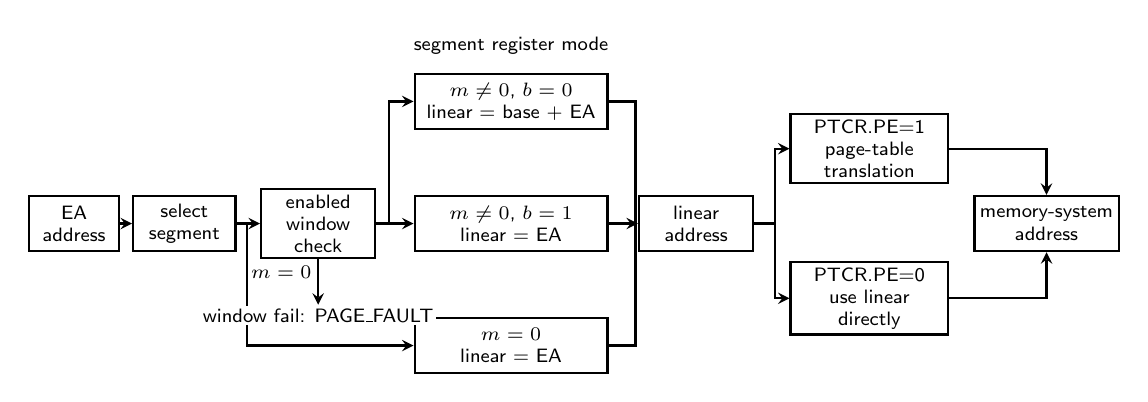
\begin{tikzpicture}[x=1cm,y=1cm,every node/.style={font=\scriptsize},>=stealth,line width=0.82pt]
\tikzset{box/.style={draw,align=center,minimum height=0.70cm,inner sep=2pt}, lab/.style={fill=white,inner sep=1pt}}
\node[box,minimum width=1.15cm] (ea) at (0.55,0) {EA\\address};
\node[box,minimum width=1.30cm] (sel) at (1.95,0) {select\\segment};
\node[box,minimum width=1.45cm] (check) at (3.65,0) {enabled\\window\\check};
\node[box,minimum width=2.45cm] (add) at (6.10,1.55) {$m\ne0$, $b=0$\\linear = base + EA};
\node[box,minimum width=2.45cm] (keep) at (6.10,0) {$m\ne0$, $b=1$\\linear = EA};
\node[box,minimum width=2.45cm] (disabled) at (6.10,-1.55) {$m=0$\\linear = EA};
\node[box,minimum width=1.45cm] (lin) at (8.45,0) {linear\\address};
\node[box,minimum width=2.00cm] (page) at (10.65,0.95) {PTCR.PE=1\\page-table\\translation};
\node[box,minimum width=2.00cm] (direct) at (10.65,-0.95) {PTCR.PE=0\\use linear\\directly};
\node[box,minimum width=1.75cm] (out) at (12.90,0) {memory-system\\address};
\draw[->] (ea.east) -- (sel.west);
\coordinate (modebranch) at (2.75,0);
\draw (sel.east) -- (modebranch);
\draw[->] (modebranch) -- (check.west);
\draw[->] (modebranch) |- node[lab,pos=0.20,right] {$m=0$} (disabled.west);
\coordinate (segbranch) at (4.55,0);
\draw[->] (check.east) -- (segbranch) |- (add.west);
\draw[->] (check.east) -- (keep.west);
\draw[->] (check.south) -- ++(0,-0.58) node[lab,below] {window fail: PAGE\_FAULT};
\coordinate (linmerge) at (7.45,0);
\draw (add.east) -- ++(0.34,0) |- (linmerge);
\draw (keep.east) -- (linmerge);
\draw (disabled.east) -- ++(0.34,0) |- (linmerge);
\draw[->] (linmerge) -- (lin.west);
\node[anchor=south] at (6.10,2.02) {segment register mode};
\coordinate (pebranch) at (9.45,0);
\draw[->] (lin.east) -- (pebranch) |- (page.west);
\draw[->] (lin.east) -- (pebranch) |- (direct.west);
\draw[->] (page.east) -| (out.north);
\draw[->] (direct.east) -| (out.south);
\end{tikzpicture}
\manualfigurecaption{Address Translation Pipeline}
\end{center}


\subsection{Translation Pipeline}
\begingroup\small
\begin{longtable}{@{}p{1.65in}p{3.85in}@{}}
\toprule
\textbf{Stage} & \textbf{Result}\\
\midrule
Effective address & address generated by the selected EA form\\
Segment pre-translation & disabled segment passes the address through; enabled segment checks a byte-addressed window with page-granular base and span\\
Linear address & segment output, or the EA directly when segmentation is disabled\\
Paging, PTCR.PE = 1 & walk page tables from PTCR.root\_page and apply PTE attributes\\
Paging, PTCR.PE = 0 & use the linear address directly\\
\bottomrule
\end{longtable}
\manualtablecaption{Table 3-1. Address Translation Stages}
\endgroup

\subsection{Combined Segment and Page Translation}
Segment pre-translation and page-table translation are composed in a fixed order.
The effective-address unit first computes an address value from the selected addressing
mode. A segment register is then selected by the access class or by an explicit
segment-qualified effective-address form. The selected segment produces the linear
address that is either used directly or passed to the paging stage.
Architectural pointer values used by ordinary code are the address values before this
segment stage. If software needs the linear address produced by segment pre-translation,
it uses \texttt{SEGLEA}; the resulting value is not the normal representation of a
portable pointer under the ABI.

\[
\begin{aligned}
\mathrm{EA} &\rightarrow \text{segment pre-translation} \rightarrow \text{linear address}\\
\texttt{PTCR.PE}=1:\quad \text{linear address} &\rightarrow \text{page walk} \rightarrow \text{memory-system address}\\
\texttt{PTCR.PE}=0:\quad \text{linear address} &\rightarrow \text{memory-system address}
\end{aligned}
\]

Instruction fetches use the code-segment context, stack accesses use the stack-segment
context, and ordinary data accesses use the data-segment context unless the effective
address explicitly selects another segment. The segment stage does not replace paging
as the memory-protection mechanism. Disabled segments perform no window check and no
base addition. Translated-window segments check an offset and add the segment base.
Bounds-only segments check an already-linear address without adding the base. In both
enabled modes, the checked byte-addressed window has a page-granular base and span.

Let \(x\) be the address produced by effective-address calculation, and let the selected
segment register define:

\[
\mathit{base} = \mathit{base\_page} \times 4096,\qquad
\mathit{span} = m \times 2^e \times 4096,\qquad
\mathit{limit} = \mathit{base} + \mathit{span}.
\]

The base, span, and limit are computed in an unsigned domain wide enough to represent
the full 64-bit linear-address space plus one. If \(\mathit{limit} > 2^{64}\), the
segment register image is invalid and any access through it reports \texttt{PAGE\_FAULT}.

\begingroup\footnotesize
\begin{longtable}{@{}p{1.15in}p{1.0in}p{1.55in}p{1.80in}@{}}
\toprule
\textbf{Mode} & \textbf{Segment State} & \textbf{Check} & \textbf{Linear Address}\\
\midrule
\endhead
disabled & \texttt{m=0} & no segment-window check & \(\mathit{linear}=x\)\\
translated window & \texttt{m!=0, b=0} & \(0 \le x < \mathit{span}\) & \(\mathit{linear}=\mathit{base}+x\)\\
bounds-only window & \texttt{m!=0, b=1} & \(\mathit{base} \le x < \mathit{limit}\) & \(\mathit{linear}=x\)\\
\bottomrule
\end{longtable}
\manualtablecaption{Segment Pre-Translation Modes}
\endgroup

The translated-window mode is useful when an address is interpreted as an offset inside
the selected segment. The bounds-only mode is useful when the effective address is already
a linear address but should still be constrained to the segment window. In both enabled
segment modes, a failed segment-window check is reported through the page-fault exception
class.

\begingroup\footnotesize
\begin{longtable}{@{}p{1.15in}p{1.05in}p{3.25in}@{}}
\toprule
\textbf{Segment Result} & \textbf{Paging State} & \textbf{Final Translation Behavior}\\
\midrule
\endhead
\(\mathit{linear}=x\) from disabled segment & \texttt{PTCR.PE=0} & The effective address is used directly as the memory-system address. PTE presence, permission, cache, and addressing-type attributes are not applied.\\
\(\mathit{linear}=x\) from disabled segment & \texttt{PTCR.PE=1} & The effective address is interpreted as a linear address. Canonical-address checking, page walk, PTE permissions, PTE cache policy, and PTE addressing type are applied.\\
\(\mathit{linear}=\mathit{base}+x\) from translated segment & \texttt{PTCR.PE=0} & The segment performs the window check and base addition. The resulting linear address is used directly by the memory system.\\
\(\mathit{linear}=\mathit{base}+x\) from translated segment & \texttt{PTCR.PE=1} & The segment first checks and translates the offset. The resulting linear address is then canonical-checked and translated through the page tables.\\
\(\mathit{linear}=x\) from bounds-only segment & either state & The segment constrains the already-linear address to the selected window. If paging is enabled, the checked linear address is then translated by the page tables; otherwise it is used directly.\\
\bottomrule
\end{longtable}
\manualtablecaption{Segment and Paging Composition}
\endgroup

When paging is enabled, PTE permissions are evaluated after segment pre-translation.
For example, an access may pass the segment-window check and still fault because the
leaf PTE is not present, is not writable for a store, is not executable for an instruction
fetch, or is not accessible at the current privilege level. Conversely, paging cannot
rescue an address that fails the enabled segment-window check, because the page walk is
not attempted for that access.

Privilege checks that do not depend on address translation are performed before page-fault
reporting. Address failures from the active translation stages, including enabled
segment-window checks, canonical-address checks when paging is enabled, page-table walks,
PTE permission checks, and stack-memory translation, are reported through the
\texttt{PAGE\_FAULT} vector.


\subsection{Segmentation Stage}
Segmentation is a page-granular address-window and pre-translation mechanism, not
the primary memory-protection mechanism. A segment with \(m = 0\) is disabled and
passes the effective-address result through unchanged. A translated segment checks
an offset against the segment span and then adds the segment base. A bounds-only
segment checks an already-linear address against the segment window without adding
the base.

\begin{align*}
\mathit{base} &= \mathit{base\_page} \times 4096\\
\mathit{span} &= m \times 2^e \times 4096\\
\mathit{limit} &= \mathit{base} + \mathit{span}\\
m=0:\quad \mathit{linear} &= x\\
m\ne0,\ b=0:\quad 0 \le x < \mathit{span},\quad \mathit{linear} &= \mathit{base}+x\\
m\ne0,\ b=1:\quad \mathit{base} \le x < \mathit{limit},\quad \mathit{linear} &= x
\end{align*}

The base, span, and limit are computed in an unsigned domain wide enough to
represent the full 64-bit linear-address space plus one. If
\(\mathit{limit} > 2^{64}\), the segment register image is invalid and any
access through it reports \texttt{PAGE\_FAULT}.

\subsection{Paging Stage}
Paging performs final address translation and supplies the protection attributes.
LA57 selects either four-level paging with 48-bit canonical linear addresses or
five-level paging with 57-bit canonical linear addresses. PTE[0..11] are
architecturally assigned low attribute bits, PTE[12..PABITS-1] contains the
physical frame number or next-table frame number, and PTE[PABITS..63] is
software-defined. Bit 10 is reserved for software use.

\clearpage
\subsection{LA48 Four-Level Paging}
When PTCR.LA57 is zero, paging uses a 48-bit canonical linear address. Bits
63..48 must be the canonical sign extension of bit 47. The remaining address
bits select four nine-bit page-table indexes followed by a twelve-bit page
offset.

\begin{center}\vspace{3pt}
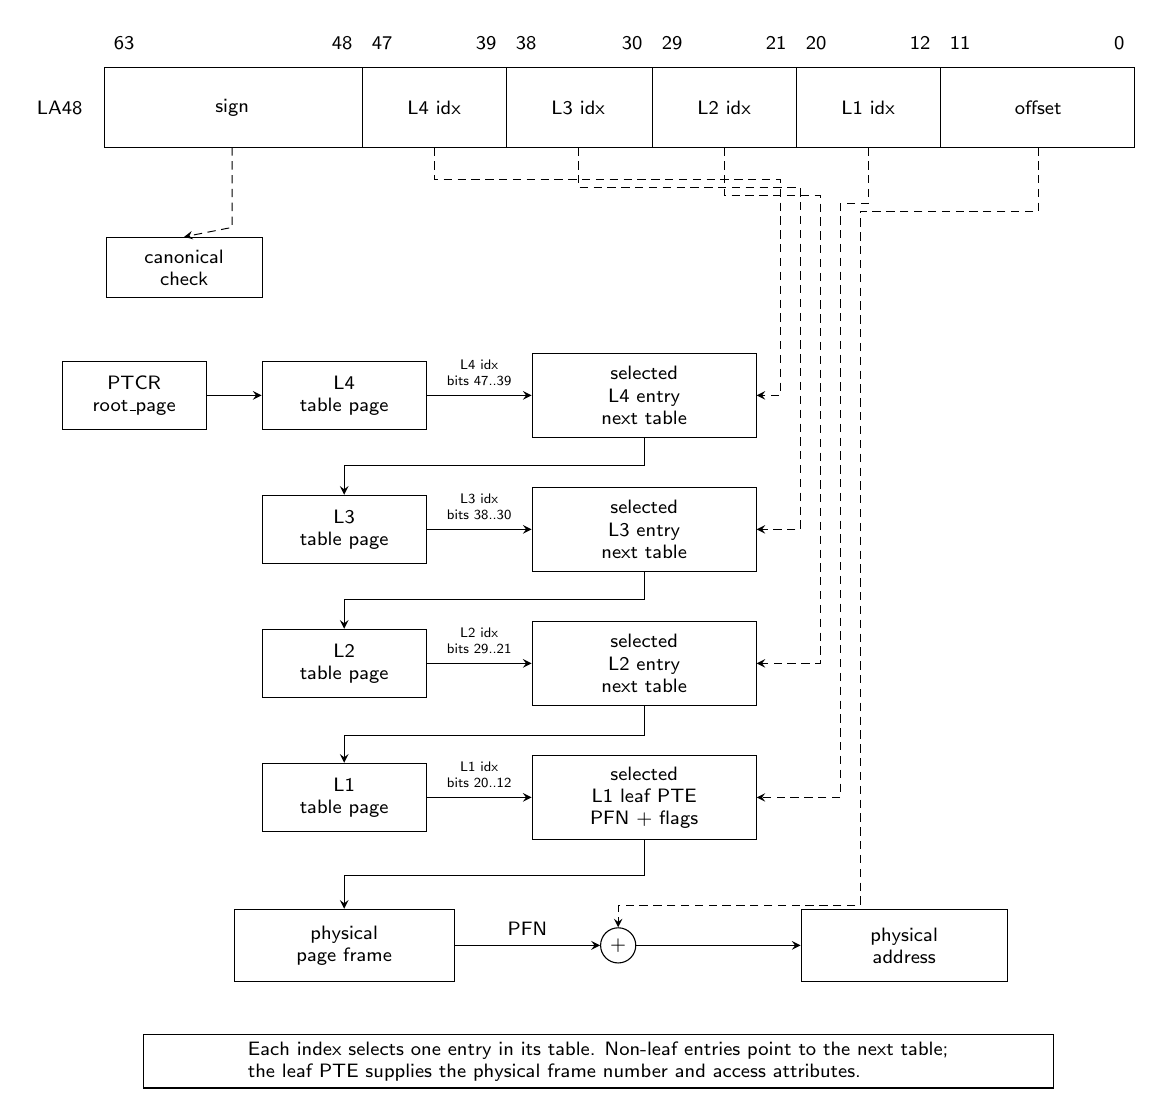
\begin{tikzpicture}[x=1in,y=1in,every node/.style={font=\scriptsize},>=stealth]
\node[anchor=east] at (0.49,6.22) {LA48};
\node[anchor=south west] at (0.55,6.46) {63};
\node[anchor=south east] at (1.84,6.46) {48};
\draw (0.55,6.02) rectangle (1.84,6.42);
\node[align=center] at (1.19,6.22) {sign};
\node[anchor=south west] at (1.84,6.46) {47};
\node[anchor=south east] at (2.56,6.46) {39};
\draw (1.84,6.02) rectangle (2.56,6.42);
\node[align=center] at (2.20,6.22) {L4 idx};
\node[anchor=south west] at (2.56,6.46) {38};
\node[anchor=south east] at (3.29,6.46) {30};
\draw (2.56,6.02) rectangle (3.29,6.42);
\node[align=center] at (2.92,6.22) {L3 idx};
\node[anchor=south west] at (3.29,6.46) {29};
\node[anchor=south east] at (4.01,6.46) {21};
\draw (3.29,6.02) rectangle (4.01,6.42);
\node[align=center] at (3.65,6.22) {L2 idx};
\node[anchor=south west] at (4.01,6.46) {20};
\node[anchor=south east] at (4.73,6.46) {12};
\draw (4.01,6.02) rectangle (4.73,6.42);
\node[align=center] at (4.37,6.22) {L1 idx};
\node[anchor=south west] at (4.73,6.46) {11};
\node[anchor=south east] at (5.70,6.46) {0};
\draw (4.73,6.02) rectangle (5.70,6.42);
\node[align=center] at (5.22,6.22) {offset};
\node[draw,align=center,minimum width=0.78in,minimum height=0.30in] (canon) at (0.95,5.42) {canonical\\check};
\draw[->,black,densely dashed,line width=0.35pt] (1.19,6.02) -- (1.19,5.62) -- (canon.north);
\node[draw,align=center,minimum width=0.82in,minimum height=0.34in,inner sep=1.5pt] (tbl0) at (1.75,4.78) {L4\\table page};
\node[draw,align=center,minimum width=1.12in,minimum height=0.42in,inner sep=1.5pt] (ent0) at (3.25,4.78) {selected\\L4 entry\\next table};
\node[draw,align=center,minimum width=0.72in,minimum height=0.34in,inner sep=1.5pt] (root) at (0.70,4.78) {PTCR\\root\_page};
\draw[->] (root.east) -- (tbl0.west);
\draw[->] (tbl0.east) -- node[above,align=center,font=\tiny] {L4 idx\\bits 47..39} (ent0.west);
\draw[->,black,densely dashed,line width=0.35pt] (2.20,6.02) -- (2.20,5.86) -- (3.93,5.86) -- (3.93,4.78) -- (ent0.east);
\node[draw,align=center,minimum width=0.82in,minimum height=0.34in,inner sep=1.5pt] (tbl1) at (1.75,4.11) {L3\\table page};
\node[draw,align=center,minimum width=1.12in,minimum height=0.42in,inner sep=1.5pt] (ent1) at (3.25,4.11) {selected\\L3 entry\\next table};
\draw[->] (ent0.south) -- (3.25,4.43) -- (1.75,4.43) -- (tbl1.north);
\draw[->] (tbl1.east) -- node[above,align=center,font=\tiny] {L3 idx\\bits 38..30} (ent1.west);
\draw[->,black,densely dashed,line width=0.35pt] (2.92,6.02) -- (2.92,5.82) -- (4.03,5.82) -- (4.03,4.11) -- (ent1.east);
\node[draw,align=center,minimum width=0.82in,minimum height=0.34in,inner sep=1.5pt] (tbl2) at (1.75,3.44) {L2\\table page};
\node[draw,align=center,minimum width=1.12in,minimum height=0.42in,inner sep=1.5pt] (ent2) at (3.25,3.44) {selected\\L2 entry\\next table};
\draw[->] (ent1.south) -- (3.25,3.76) -- (1.75,3.76) -- (tbl2.north);
\draw[->] (tbl2.east) -- node[above,align=center,font=\tiny] {L2 idx\\bits 29..21} (ent2.west);
\draw[->,black,densely dashed,line width=0.35pt] (3.65,6.02) -- (3.65,5.78) -- (4.13,5.78) -- (4.13,3.44) -- (ent2.east);
\node[draw,align=center,minimum width=0.82in,minimum height=0.34in,inner sep=1.5pt] (tbl3) at (1.75,2.77) {L1\\table page};
\node[draw,align=center,minimum width=1.12in,minimum height=0.42in,inner sep=1.5pt] (ent3) at (3.25,2.77) {selected\\L1 leaf PTE\\PFN + flags};
\draw[->] (ent2.south) -- (3.25,3.08) -- (1.75,3.08) -- (tbl3.north);
\draw[->] (tbl3.east) -- node[above,align=center,font=\tiny] {L1 idx\\bits 20..12} (ent3.west);
\draw[->,black,densely dashed,line width=0.35pt] (4.37,6.02) -- (4.37,5.74) -- (4.23,5.74) -- (4.23,2.77) -- (ent3.east);
\node[draw,align=center,minimum width=1.10in,minimum height=0.36in] (frame) at (1.75,2.03) {physical\\page frame};
\draw[->] (ent3.south) -- (3.25,2.38) -- (1.75,2.38) -- (frame.north);
\node[draw,circle,inner sep=1.8pt] (plus) at (3.12,2.03) {+};
\node[draw,align=center,minimum width=1.03in,minimum height=0.36in] (phys) at (4.55,2.03) {physical\\address};
\draw[->] (frame.east) -- node[above] {PFN} (plus.west);
\draw[->] (plus.east) -- (phys.west);
\draw[->,black,densely dashed,line width=0.35pt] (5.22,6.02) -- (5.22,5.70) -- (4.33,5.70) -- (4.33,2.23) -- (3.12,2.23) -- (plus.north);
\node[draw,align=left,minimum width=4.55in,inner sep=2.5pt] at (3.02,1.45) {Each index selects one entry in its table. Non-leaf entries point to the next table;\\the leaf PTE supplies the physical frame number and access attributes.};
\end{tikzpicture}
\manualfigurecaption{LA48 Four-Level Page Walk}
\end{center}



\clearpage
\subsection{LA57 Five-Level Paging}
When PTCR.LA57 is one, paging uses a 57-bit canonical linear address. Bits
63..57 must be the canonical sign extension of bit 56. The additional L5 index
selects the top-level table before the same L4 through L1 walk used by LA48.

\begin{center}\vspace{3pt}
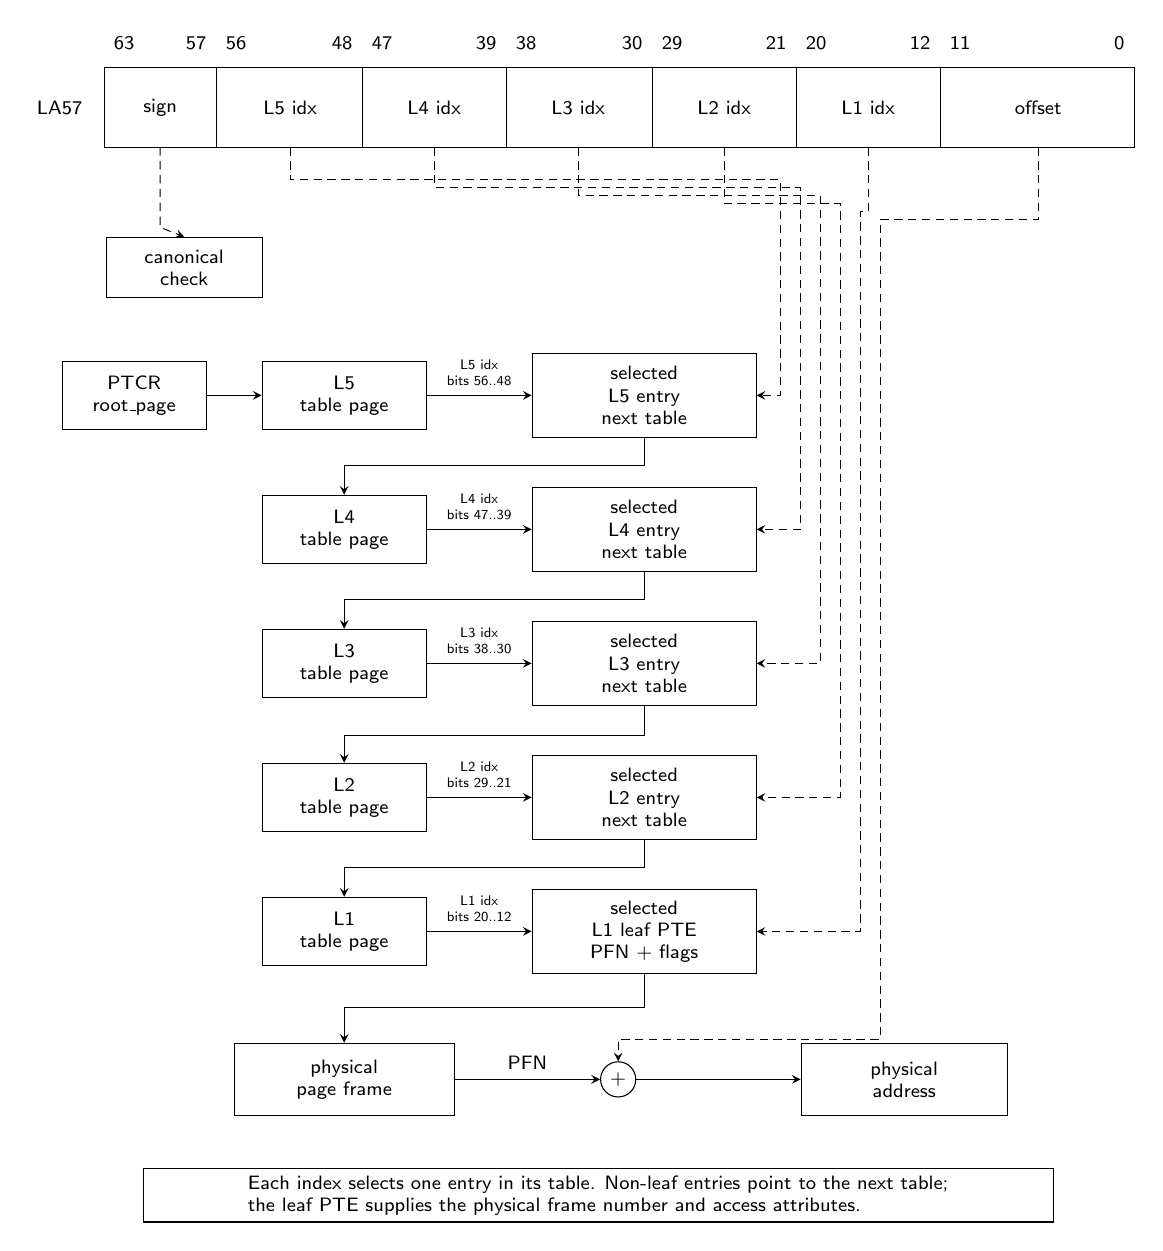
\begin{tikzpicture}[x=1in,y=1in,every node/.style={font=\scriptsize},>=stealth]
\node[anchor=east] at (0.49,6.22) {LA57};
\node[anchor=south west] at (0.55,6.46) {63};
\node[anchor=south east] at (1.11,6.46) {57};
\draw (0.55,6.02) rectangle (1.11,6.42);
\node[align=center] at (0.83,6.22) {sign};
\node[anchor=south west] at (1.11,6.46) {56};
\node[anchor=south east] at (1.84,6.46) {48};
\draw (1.11,6.02) rectangle (1.84,6.42);
\node[align=center] at (1.48,6.22) {L5 idx};
\node[anchor=south west] at (1.84,6.46) {47};
\node[anchor=south east] at (2.56,6.46) {39};
\draw (1.84,6.02) rectangle (2.56,6.42);
\node[align=center] at (2.20,6.22) {L4 idx};
\node[anchor=south west] at (2.56,6.46) {38};
\node[anchor=south east] at (3.29,6.46) {30};
\draw (2.56,6.02) rectangle (3.29,6.42);
\node[align=center] at (2.92,6.22) {L3 idx};
\node[anchor=south west] at (3.29,6.46) {29};
\node[anchor=south east] at (4.01,6.46) {21};
\draw (3.29,6.02) rectangle (4.01,6.42);
\node[align=center] at (3.65,6.22) {L2 idx};
\node[anchor=south west] at (4.01,6.46) {20};
\node[anchor=south east] at (4.73,6.46) {12};
\draw (4.01,6.02) rectangle (4.73,6.42);
\node[align=center] at (4.37,6.22) {L1 idx};
\node[anchor=south west] at (4.73,6.46) {11};
\node[anchor=south east] at (5.70,6.46) {0};
\draw (4.73,6.02) rectangle (5.70,6.42);
\node[align=center] at (5.22,6.22) {offset};
\node[draw,align=center,minimum width=0.78in,minimum height=0.30in] (canon) at (0.95,5.42) {canonical\\check};
\draw[->,black,densely dashed,line width=0.35pt] (0.83,6.02) -- (0.83,5.62) -- (canon.north);
\node[draw,align=center,minimum width=0.82in,minimum height=0.34in,inner sep=1.5pt] (tbl0) at (1.75,4.78) {L5\\table page};
\node[draw,align=center,minimum width=1.12in,minimum height=0.42in,inner sep=1.5pt] (ent0) at (3.25,4.78) {selected\\L5 entry\\next table};
\node[draw,align=center,minimum width=0.72in,minimum height=0.34in,inner sep=1.5pt] (root) at (0.70,4.78) {PTCR\\root\_page};
\draw[->] (root.east) -- (tbl0.west);
\draw[->] (tbl0.east) -- node[above,align=center,font=\tiny] {L5 idx\\bits 56..48} (ent0.west);
\draw[->,black,densely dashed,line width=0.35pt] (1.48,6.02) -- (1.48,5.86) -- (3.93,5.86) -- (3.93,4.78) -- (ent0.east);
\node[draw,align=center,minimum width=0.82in,minimum height=0.34in,inner sep=1.5pt] (tbl1) at (1.75,4.11) {L4\\table page};
\node[draw,align=center,minimum width=1.12in,minimum height=0.42in,inner sep=1.5pt] (ent1) at (3.25,4.11) {selected\\L4 entry\\next table};
\draw[->] (ent0.south) -- (3.25,4.43) -- (1.75,4.43) -- (tbl1.north);
\draw[->] (tbl1.east) -- node[above,align=center,font=\tiny] {L4 idx\\bits 47..39} (ent1.west);
\draw[->,black,densely dashed,line width=0.35pt] (2.20,6.02) -- (2.20,5.82) -- (4.03,5.82) -- (4.03,4.11) -- (ent1.east);
\node[draw,align=center,minimum width=0.82in,minimum height=0.34in,inner sep=1.5pt] (tbl2) at (1.75,3.44) {L3\\table page};
\node[draw,align=center,minimum width=1.12in,minimum height=0.42in,inner sep=1.5pt] (ent2) at (3.25,3.44) {selected\\L3 entry\\next table};
\draw[->] (ent1.south) -- (3.25,3.76) -- (1.75,3.76) -- (tbl2.north);
\draw[->] (tbl2.east) -- node[above,align=center,font=\tiny] {L3 idx\\bits 38..30} (ent2.west);
\draw[->,black,densely dashed,line width=0.35pt] (2.92,6.02) -- (2.92,5.78) -- (4.13,5.78) -- (4.13,3.44) -- (ent2.east);
\node[draw,align=center,minimum width=0.82in,minimum height=0.34in,inner sep=1.5pt] (tbl3) at (1.75,2.77) {L2\\table page};
\node[draw,align=center,minimum width=1.12in,minimum height=0.42in,inner sep=1.5pt] (ent3) at (3.25,2.77) {selected\\L2 entry\\next table};
\draw[->] (ent2.south) -- (3.25,3.08) -- (1.75,3.08) -- (tbl3.north);
\draw[->] (tbl3.east) -- node[above,align=center,font=\tiny] {L2 idx\\bits 29..21} (ent3.west);
\draw[->,black,densely dashed,line width=0.35pt] (3.65,6.02) -- (3.65,5.74) -- (4.23,5.74) -- (4.23,2.77) -- (ent3.east);
\node[draw,align=center,minimum width=0.82in,minimum height=0.34in,inner sep=1.5pt] (tbl4) at (1.75,2.10) {L1\\table page};
\node[draw,align=center,minimum width=1.12in,minimum height=0.42in,inner sep=1.5pt] (ent4) at (3.25,2.10) {selected\\L1 leaf PTE\\PFN + flags};
\draw[->] (ent3.south) -- (3.25,2.42) -- (1.75,2.42) -- (tbl4.north);
\draw[->] (tbl4.east) -- node[above,align=center,font=\tiny] {L1 idx\\bits 20..12} (ent4.west);
\draw[->,black,densely dashed,line width=0.35pt] (4.37,6.02) -- (4.37,5.70) -- (4.33,5.70) -- (4.33,2.10) -- (ent4.east);
\node[draw,align=center,minimum width=1.10in,minimum height=0.36in] (frame) at (1.75,1.36) {physical\\page frame};
\draw[->] (ent4.south) -- (3.25,1.72) -- (1.75,1.72) -- (frame.north);
\node[draw,circle,inner sep=1.8pt] (plus) at (3.12,1.36) {+};
\node[draw,align=center,minimum width=1.03in,minimum height=0.36in] (phys) at (4.55,1.36) {physical\\address};
\draw[->] (frame.east) -- node[above] {PFN} (plus.west);
\draw[->] (plus.east) -- (phys.west);
\draw[->,black,densely dashed,line width=0.35pt] (5.22,6.02) -- (5.22,5.66) -- (4.43,5.66) -- (4.43,1.56) -- (3.12,1.56) -- (plus.north);
\node[draw,align=left,minimum width=4.55in,inner sep=2.5pt] at (3.02,0.78) {Each index selects one entry in its table. Non-leaf entries point to the next table;\\the leaf PTE supplies the physical frame number and access attributes.};
\end{tikzpicture}
\manualfigurecaption{LA57 Five-Level Page Walk}
\end{center}



\clearpage
\subsection{Page-Table Entry Format}
\begin{manuallistedbitdiagram}{PTE Low Attribute Bits}
\manualbitfieldrow{PTE[11:0]}{%
\manualbitlabel{11}
\manualbitlabel{7}
\manualbitlabel{0}
}{%
\manualbitfieldtext{T}{1}
\manualbitfieldtext{SW0}{1}
\manualbitfieldtext{CP}{2}
\manualbitfieldtext{AT}{1}
\manualbitfieldtext{D}{1}
\manualbitfieldtext{A}{1}
\manualbitfieldtext{G}{1}
\manualbitfieldtext{U}{1}
\manualbitfieldtext{X}{1}
\manualbitfieldtext{W}{1}
\manualbitfieldtext{P}{1}
}
\end{manuallistedbitdiagram}



\begin{manuallongtable}{@{}>{\raggedright\arraybackslash}p{0.55in}>{\raggedright\arraybackslash}p{0.65in}>{\raggedright\arraybackslash}p{4.25in}@{}}
\toprule
\textbf{Field} & \textbf{Bits} & \textbf{Meaning}\\
\midrule
\endhead
\texttt{T} & 11 & Table / non-leaf entry\\
\texttt{SW0} & 10 & Software-defined\\
\texttt{CP} & 9:8 & Cache policy\\
\texttt{AT} & 7 & Addressing type\\
\texttt{D} & 6 & Dirty\\
\texttt{A} & 5 & Accessed\\
\texttt{G} & 4 & Global TLB entry\\
\texttt{U} & 3 & User accessible\\
\texttt{X} & 2 & Executable\\
\texttt{W} & 1 & Writable\\
\texttt{P} & 0 & Present\\
\bottomrule
\end{manuallongtable}
\manualtablecaption{Page-Table Entry Low Attribute Bits}


\begin{manuallongtable}{@{}>{\raggedright\arraybackslash}p{1.15in}>{\raggedright\arraybackslash}p{4.35in}@{}}
\toprule
\textbf{Level} & \textbf{Rule}\\
\midrule
\endhead
large pages & unsupported\\
non leaf levels & for every level above L1, P must be 1 and T must be 1; any other value causes PAGE\_FAULT\\
leaf level & at L1, P must be 1 and T must be 0; any other value causes PAGE\_FAULT\\
\bottomrule
\end{manuallongtable}
\manualtablecaption{Page-Walk Level Rules}


\begin{manuallongtable}{@{}>{\raggedright\arraybackslash}p{0.95in}>{\raggedright\arraybackslash}p{4.55in}@{}}
\toprule
\textbf{Field} & \textbf{Rule}\\
\midrule
\endhead
\begin{tabular}[t]{@{}l@{}}non-leaf\\\texttt{PFN}\end{tabular} & physical frame number of the next-level table\\
\begin{tabular}[t]{@{}l@{}}non-leaf\\\texttt{W\_X\_U}\end{tabular} & constrain descendant leaf permissions; access is allowed only if every traversed entry and the leaf permit the requested access\\
\begin{tabular}[t]{@{}l@{}}non-leaf\\\texttt{A}\end{tabular} & set when the entry is successfully traversed\\
\begin{tabular}[t]{@{}l@{}}non-leaf\\\texttt{D}\end{tabular} & leaf-only, must be zero in non-leaf entries\\
\begin{tabular}[t]{@{}l@{}}non-leaf\\\texttt{G}\end{tabular} & leaf-only, must be zero in non-leaf entries\\
\begin{tabular}[t]{@{}l@{}}non-leaf\\\texttt{CP}\end{tabular} & cache policy used for hardware table-walk memory accesses to the next-level table\\
\begin{tabular}[t]{@{}l@{}}non-leaf\\\texttt{AT}\end{tabular} & must be 0 for non-leaf entries; page tables are byte-addressed memory\\
\begin{tabular}[t]{@{}l@{}}non-leaf\\\texttt{SW0}\end{tabular} & software-defined and ignored by hardware\\
\begin{tabular}[t]{@{}l@{}}leaf\\\texttt{PFN}\end{tabular} & physical frame number of the mapped page\\
\begin{tabular}[t]{@{}l@{}}leaf\\\texttt{W\_X\_U}\end{tabular} & access permissions for stores, instruction fetches, and user-mode access\\
\begin{tabular}[t]{@{}l@{}}leaf\\\texttt{A}\end{tabular} & set when the leaf mapping is successfully used\\
\begin{tabular}[t]{@{}l@{}}leaf\\\texttt{D}\end{tabular} & set on a successful store through the leaf mapping\\
\begin{tabular}[t]{@{}l@{}}leaf\\\texttt{G}\end{tabular} & marks the resulting translation as global\\
\begin{tabular}[t]{@{}l@{}}leaf\\\texttt{CP}\end{tabular} & cache policy for the mapped access\\
\begin{tabular}[t]{@{}l@{}}leaf\\\texttt{AT}\end{tabular} & addressing type for the mapped access; does not change PFN plus offset address formation\\
\begin{tabular}[t]{@{}l@{}}leaf\\\texttt{SW0}\end{tabular} & software-defined and ignored by hardware\\
\bottomrule
\end{manuallongtable}
\manualtablecaption{PTE Attribute Semantics}


\begin{manuallongtable}{@{}>{\raggedright\arraybackslash}p{0.85in}>{\raggedright\arraybackslash}p{2.35in}>{\raggedright\arraybackslash}p{2.30in}@{}}
\toprule
\textbf{Mode} & \textbf{Condition} & \textbf{Result}\\
\midrule
\endhead
user & effective U permission is 0 & PRIVILEGE\_FAULT\\
user & effective U permission is 1 & allowed subject to present, W/X, and access-type checks\\
supervisor & effective U permission is 0 & allowed for C-domain accesses subject to present, W/X, and access-type checks\\
supervisor & effective U permission is 1 and access domain is C & PAGE\_FAULT\\
supervisor & effective U permission is 1 and access domain is U & allowed subject to present, W/X, and access-type checks\\
supervisor & effective U permission is 0 and access domain is U & PAGE\_FAULT\\
\bottomrule
\end{manuallongtable}
\manualtablecaption{PTE User-Permission Rules}


\clearpage
\section{Memory Model}
\subsection{Scope}
The memory model defines the architectural behavior of instruction fetches, loads,
stores, atomic read-modify-write operations, cache maintenance, and translation-cache
maintenance after effective-address calculation and address translation. Language
rules such as C \texttt{volatile}, C atomics, and process startup policy are ABI
concerns; this section describes the guarantees provided directly by the ISA.

\subsection{Memory Access Domains}
All instruction fetch, data, stack, and device accesses use the same effective-address
and address-translation pipeline. The final page-table attributes classify the access
domain.

\begingroup\footnotesize
\begin{longtable}{@{}p{1.25in}p{1.55in}p{2.7in}@{}}
\toprule
\textbf{Attribute} & \textbf{Domain} & \textbf{Architectural Meaning}\\
\midrule
\endhead
\texttt{PTE.AT=0} & byte-addressed memory & Normal memory is addressed in bytes and may be cached according to \texttt{PTE.CP}.\\
\texttt{PTE.AT=1} & externally acknowledged memory & The access is acknowledged by an external memory or device agent and may have bus-sized side effects.\\
\texttt{PTE.CP=00} & cacheable & Normal coherent cacheable memory.\\
\texttt{PTE.CP=01} & uncacheable & Accesses are not allocated into normal data caches.\\
\texttt{PTE.CP=10} & write-through & Stores become visible through a write-through cache policy.\\
\texttt{PTE.CP=11} & write-combining & Stores may be gathered and combined before visibility; explicit ordering is required when software depends on completion order.\\
\bottomrule
\end{longtable}
\manualtablecaption{Memory Access Domains}
\endgroup

Externally acknowledged memory is not treated as ordinary cacheable memory. An implementation
must not silently replace an externally acknowledged access with an unrelated cached access.
The translated address is still formed as PFN plus page offset; \texttt{PTE.AT=1}
changes the memory transaction domain and acknowledgement behavior, not the address
arithmetic. Ordering requirements for device protocols are expressed with mapped memory
attributes and explicit fence or cache-synchronization instructions.

\subsection{Access Size, Alignment, and Tearing}
The architectural scalar memory sizes are byte, word, long word, and quad word. A memory
access of size \(N\) bytes is naturally aligned when its byte address is a multiple of \(N\).

\begingroup\footnotesize
\begin{longtable}{@{}p{0.75in}p{0.85in}p{1.25in}p{2.65in}@{}}
\toprule
\textbf{Suffix} & \textbf{Bytes} & \textbf{Natural Alignment} & \textbf{Tear-Free Guarantee}\\
\midrule
\endhead
\texttt{B} & 1 & any byte address & aligned normal-memory load/store is tear-free\\
\texttt{W} & 2 & address divisible by 2 & aligned normal-memory load/store is tear-free\\
\texttt{L} & 4 & address divisible by 4 & aligned normal-memory load/store is tear-free\\
\texttt{Q} & 8 & address divisible by 8 & aligned normal-memory load/store is tear-free\\
\bottomrule
\end{longtable}
\manualtablecaption{Scalar Access Sizes and Alignment}
\endgroup

Unaligned ordinary memory accesses are architecturally permitted. An unaligned load or
store does not fault merely because of its alignment, although it may still fault because
one of the bytes it touches fails address translation, permission checking, or device
acknowledgement. Unaligned accesses may be implemented as multiple aligned memory beats
and have no tear-free or atomicity guarantee.

Architectural accesses wider than eight bytes, including block transfers and repeated
string-like operations, are not single atomic memory accesses. They are described as a
sequence of scalar accesses unless a specific instruction form states otherwise.

\subsection{Atomic Access Requirements}
Atomic instructions require a naturally aligned memory operand for the selected operand
size. A misaligned atomic memory operand is invalid for the atomic operation and must not
complete as a non-atomic read-modify-write. If a fault is reported for such an instruction,
the fault is precise and the atomic memory location is not updated.

For an aligned atomic read-modify-write instruction, the read, modification, and write of
the selected memory location are observed as one indivisible operation by other agents that
can access the same physical location. Atomic read-modify-write instructions carry a
memory-order selector as part of the atomic instruction format. The selector constrains
visibility ordering around the indivisible update; it is not a general-purpose prefix.

\begin{manuallongtable}{@{}>{\raggedright\arraybackslash}p{0.9in}>{\raggedright\arraybackslash}p{0.75in}>{\raggedright\arraybackslash}p{3.8in}@{}}
\toprule
\textbf{Selector} & \textbf{Code} & \textbf{Architectural Ordering Effect}\\
\midrule
\endhead
\texttt{RELAXED} & \texttt{0} & Atomicity only. No ordering is imposed on unrelated memory operations.\\
\texttt{ACQUIRE} & \texttt{1} & Later memory operations by the same hardware thread are ordered after the atomic operation.\\
\texttt{RELEASE} & \texttt{2} & Earlier memory operations by the same hardware thread are ordered before the atomic operation.\\
\texttt{ACQREL} & \texttt{3} & Applies both acquire and release ordering.\\
\texttt{SEQCST} & \texttt{4} & Applies acquire-release ordering and participates in the global sequentially consistent order for atomic operations.\\
RESERVED5 & \texttt{5} & Reserved selector encoding; using it is invalid for the atomic form.\\
RESERVED6 & \texttt{6} & Reserved selector encoding; using it is invalid for the atomic form.\\
RESERVED7 & \texttt{7} & Reserved selector encoding; using it is invalid for the atomic form.\\
\bottomrule
\end{manuallongtable}
\manualtablecaption{Atomic Memory-Order Selectors}


The \texttt{consume} memory order is not a separate architectural selector. Software that
needs consume-style source semantics uses the acquire selector. A full ordering point for
ordinary unrelated accesses can also be expressed with \texttt{AFENCE} when the program
needs one independently of an atomic operation.

\subsection{Visibility and Ordering}
Normal cacheable memory is coherent at the architectural level: once a store becomes visible
to another agent, later coherent accesses to the same physical location observe a value
consistent with the coherence order for that location. The ISA does not require independent
ordinary loads and stores to become visible to other agents in program order unless an
instruction dependency, an atomic operation, or a fence instruction imposes that order.

\begingroup\footnotesize
\begin{longtable}{@{}p{0.95in}p{4.45in}@{}}
\toprule
\textbf{Instruction} & \textbf{Ordering Effect}\\
\midrule
\endhead
\texttt{RFENCE} & Orders prior reads before later reads issued by the same hardware thread.\\
\texttt{WFENCE} & Orders prior writes before later writes issued by the same hardware thread.\\
\texttt{AFENCE} & Orders prior memory operations before later memory operations issued by the same hardware thread.\\
\bottomrule
\end{longtable}
\manualtablecaption{Fence Instructions}
\endgroup

Fence instructions constrain visibility ordering. They do not perform cache-line writeback,
cache invalidation, TLB invalidation, or instruction-cache synchronization by themselves
unless the instruction description explicitly says so.

\subsection{Fault and Partial-Commit Rules}
Memory faults are precise with respect to the faulting instruction. A faulting load does
not update its destination register. A faulting scalar store does not commit bytes of that
store. Atomic read-modify-write instructions either complete the whole aligned atomic
operation or leave the memory location unchanged.

Repeated operations commit completed instruction bodies only. For \texttt{REPcc}, a
completed terminating iteration whose repeat condition is false still commits the
instruction body's ordinary side effects, but it does not update the repeat counter. If a
\texttt{REP} or \texttt{REPcc} operation faults after some iterations have completed, the
completed iterations remain committed and the saved restart state describes the remaining
work.
\texttt{REPG} uses the same precise-fault rule, extended to the current grouped
iteration: completed prior group instructions in the faulting iteration remain
committed, later group instructions do not execute, and the counter is not
updated until the whole group iteration succeeds. The repeat-fault auxiliary
state allows return from the fault to continue at the faulting grouped
instruction under the active REPG context.

\subsection{Instruction Fetch and Self-Modifying Code}
Stores to memory that is later executed as instructions are ordinary data stores until an
explicit synchronization sequence makes the modified bytes visible to instruction fetch.
Code patching, dynamic relocation into executable mappings, and JIT-style code generation
therefore require instruction/data cache synchronization before execution may rely on the
new instruction bytes.

\texttt{SYNCCACHE} synchronizes instruction/data cache visibility for modified executable
memory. \texttt{INVICACHE}, \texttt{INVDCACHE}, \texttt{FLSHDCACHE}, and \texttt{WRBKDCACHE}
provide explicit cache-maintenance operations for the cache block or range selected by their
operands.

\subsection{Address-Translation Coherency}
Page-table memory is ordinary memory until a page-table update is made visible to the
translation machinery. Software that modifies page tables must order the page-table stores
before invalidating or replacing translation-cache entries. \texttt{INVTLB}, \texttt{INVPAGE},
\texttt{INVASID}, \texttt{SWPT}, and \texttt{SWPTA} define the architectural translation-cache
maintenance operations.

When ASID matching is enabled, address-space identifiers participate in translation-cache
lookup. Global entries are matched according to the page-table attributes described in the
Memory Address Translation section. When ASID matching is disabled, translation-cache entries
are matched without an address-space identifier.

\clearpage
\section{Supervisor / Privileged Programming Model}
The privileged programming model defines how execution moves between user mode and supervisor mode,
which saved state is used for return, and which control state is directly accessible.

\subsection{Privileged Model Rules}
The following rules define the supervisor and exception-control behavior used by the rest of this manual.

\begin{manuallongtable}{@{}>{\raggedright\arraybackslash}p{0.35in}>{\raggedright\arraybackslash}p{1.45in}>{\raggedright\arraybackslash}p{3.65in}@{}}
\toprule
\textbf{No.} & \textbf{Subject} & \textbf{Rule}\\
\midrule
\endhead
1 & privilege mode encoding & STATUS.PM=0 is user mode; STATUS.PM=1 is supervisor mode\\
2 & user-memory access control & Supervisor-mode memory accesses use the current-domain C by default; U2C, C2U, and U2U prefixes select user-domain access for the annotated memory operands of that instruction only\\
3 & saved STATUS return & STATUS is restored verbatim from the saved frame image; SYSCALL, trap, interrupt, and exception entry set STATUS.PM=1 only and do not mask interrupts\\
4 & supervisor entry DBANK normalization & SYSCALL, trap, interrupt, and exception entry save the interrupted DBANK selector and then set DBANK=0 before fetching the handler\\
5 & SYSCALL frame and entry & SYSCALL saves FRAME\_CONTROL, SS:SP, CS:PC, and DS, then sets DBANK=0 and uses a 32-byte supervisor-entry table with 16-byte entry-address alignment\\
6 & return instruction split & SYSRET is only for SYSCALL return; IRET is for interrupt, trap, and exception return\\
7 & IRET restore policy & IRET restores all saved interrupt-frame state and does not validate FRAME\_CONTROL.frame\_type\\
8 & malformed return frames & malformed frames are software errors and do not raise a separate architectural exception\\
9 & NMI and double-fault stacks & NMI and DOUBLE\_FAULT use the SN field of their IVT entries\\
10 & interrupt nesting limit & when hidden\_current\_idepth equals ICR.MAX\_IDEPTH, maskable interrupts are implicitly masked\\
11 & control-register access & RDCR and WRCR are always privileged; user-visible control state uses dedicated gated instructions\\
12 & reserved CPU vectors & reserved CPU vectors have no frame type; attempted delivery immediately becomes DOUBLE\_FAULT\\
\bottomrule
\end{manuallongtable}
\manualtablecaption{Privileged Model Rules}


\subsection{Privilege State}
\texttt{STATUS.PM} selects the current privilege level. Memory operands use the current-domain \texttt{C}
by default. In supervisor mode, operand annotations such as \texttt{U:[A0]} select user-domain
access for that instruction only through the encoded \texttt{U2C}, \texttt{C2U}, or \texttt{U2U} prefix.
In user mode \texttt{C} and \texttt{U} are identical, so these prefixes have no additional
architectural effect.

\begin{manuallongtable}{@{}>{\raggedright\arraybackslash}p{1.15in}>{\raggedright\arraybackslash}p{0.55in}>{\raggedright\arraybackslash}p{3.75in}@{}}
\toprule
\textbf{Field} & \textbf{Value} & \textbf{Meaning}\\
\midrule
\endhead
\texttt{STATUS.PM} & \texttt{0} & user mode\\
\texttt{STATUS.PM} & \texttt{1} & supervisor mode\\
\texttt{access domain} & \texttt{C} & current privilege-mode memory access domain\\
\texttt{access domain} & \texttt{U} & user memory access domain selected per instruction by U2C, C2U, or U2U\\
\bottomrule
\end{manuallongtable}
\manualtablecaption{Privilege State and Access Domains}


\subsection{SYSCALL and SYSRET}
\texttt{SYSCALL} is an explicit supervisor-entry path rather than an IVT-vector event. It behaves like an
extended long call: it saves the user control state, uses a 32-byte supervisor-entry table with 16-byte
entry-address alignment, loads the supervisor entry state from SPC/SCS/SDS, and sets STATUS.PM to
supervisor mode. \texttt{SYSRET} is the matching return instruction and is only for this syscall frame shape.

\begin{manuallongtable}{@{}>{\raggedright\arraybackslash}p{1.55in}>{\raggedright\arraybackslash}p{3.90in}@{}}
\toprule
\textbf{Property} & \textbf{Rule}\\
\midrule
\endhead
Entry vector & none\\
Entry target & SPC, SCS, SDS\\
Frame style & expanded long-call frame\\
Saved state & FRAME CONTROL, SS:SP, CS:PC, DS\\
Entry table size & 32 bytes\\
Entry address alignment & 16 bytes\\
Entry STATUS change & set STATUS.PM to 1 only\\
Entry DBANK change & save interrupted DBANK selector and set DBANK to 0\\
Return instruction & \texttt{SYSRET}\\
Return policy & read the syscall frame as written, restore saved DBANK, and return\\
\bottomrule
\end{manuallongtable}
\manualtablecaption{SYSCALL/SYSRET Rules}


\subsection{Interrupt and Control-State Rules}
Trap, interrupt, and exception entry also set STATUS.PM to supervisor mode, but do not automatically mask
interrupts. The saved STATUS image is restored verbatim by the matching return path. Malformed return
frames are software errors; the architecture does not raise a second exception merely because the return
frame is nonsensical.

\begin{manuallongtable}{@{}>{\raggedright\arraybackslash}p{1.65in}>{\raggedright\arraybackslash}p{3.80in}@{}}
\toprule
\textbf{Rule} & \textbf{Meaning}\\
\midrule
\endhead
Entry STATUS update & set STATUS.PM to 1\\
Entry DBANK update & save interrupted DBANK selector and set DBANK to 0\\
Saved STATUS return & restored verbatim from the saved frame image\\
Entry interrupt masking & no automatic masking\\
Interrupt stack selection & IVT entry SN selects SSSn:SSPn\\
NMI stack selection & use the IVT entry SN field\\
Double-fault stack selection & use the IVT entry SN field\\
Interrupt frame save & atomic\\
\texttt{SYSRET} & syscall frame only; restores saved DBANK from the syscall frame\\
\texttt{IRET} & restore all saved interrupt frame state including DBANK; frame\_type is not validated by hardware\\
Malformed return frame & software error; no architectural exception is raised\\
\texttt{ICR.MAX\_IDEPTH} & when hidden\_current\_idepth equals ICR.MAX\_IDEPTH, maskable interrupts are implicitly masked\\
\texttt{RDCR/WRCR} & RDCR = supervisor; WRCR = supervisor\\
User-visible control state & user-visible control state must use dedicated instructions gated by control-register policy bits\\
\bottomrule
\end{manuallongtable}
\manualtablecaption{Privileged Execution Rules}


\clearpage
\section{Exception Processing Reference}
Exception processing covers synchronous restartable CPU exceptions, traps, NMIs, external interrupts, and the
supervisor-entry state needed to return from them. The processor records a restartable context for CPU exceptions;
the operating system decides whether that context is retried, emulated, reported, or terminated. ICR selects the
interrupt vector table page and controls interrupt nesting; each IVT entry selects a handler and one of the
supervisor stack banks.

\subsection{Interrupt Vector Table}
The interrupt vector table occupies one 4096-byte page selected by \texttt{ICR.ivt\_page}. It contains 256 fixed-size
entries, each 16 bytes. The vector number selects the entry at \texttt{ICR.ivt\_page * 4096 + vector * 16}.

\begin{manuallistedformatdiagram}{Interrupt Vector Table Entry}{3}
\manualformatrowrange{entry bytes}{15}{0}{%
\manualformatfield{reserved}{7}
\manualformatfield{control}{1}
\manualformatfield{handler address}{8}
}
\end{manuallistedformatdiagram}


Bytes 0 through 7 contain the 64-bit interrupt handler address. Byte 8 is the entry control byte.
HP is the handler-present bit; if it is clear, delivery immediately becomes \texttt{DOUBLE\_FAULT}. SN selects one of
four interrupt stack banks, SSS0:SSP0 through SSS3:SSP3. Byte 8 bit 1 and bits 7 through 4 are reserved,
and bytes 9 through 15 are reserved.

\begin{manuallistedformatdiagram}{IVT Entry Control Byte}{2}
\manualformatrowrange{byte 8}{7}{0}{%
\manualformatfield{reserved}{4}
\manualformatfield{SN}{2}
\manualformatfield{0}{1}
\manualformatfield{HP}{1}
}
\end{manuallistedformatdiagram}


\begin{manuallongtable}{@{}>{\raggedright\arraybackslash}p{0.95in}>{\raggedright\arraybackslash}p{0.85in}>{\raggedright\arraybackslash}p{3.65in}@{}}
\toprule
\textbf{Field} & \textbf{Location} & \textbf{Meaning}\\
\midrule
\endhead
\texttt{handler\_address} & bytes 0..7 & interrupt handler address\\
\texttt{HP} & byte 8 bit 0 & handler present; if clear, delivery becomes DOUBLE\_FAULT\\
\texttt{reserved\_low} & byte 8 bit 1 & reserved, must be zero\\
\texttt{SN} & byte 8 bit 3:2 & \begin{tabular}[t]{@{}l@{}}selects SSSn:SSPn interrupt stack set\\0 = SSS0:SSP0\\1 = SSS1:SSP1\\2 = SSS2:SSP2\\3 = SSS3:SSP3\end{tabular}\\
\texttt{reserved\_high} & byte 8 bit 7:4 & reserved, must be zero\\
\texttt{reserved} & bytes 9..15 & reserved, must be zero\\
\bottomrule
\end{manuallongtable}
\manualtablecaption{Interrupt Vector Table Entry Fields}


\Needspace{3.4in}
\subsection{Vector Assignment}
Vectors 0x00..0x1F are owned by the CPU architecture. Assigned CPU vectors are grouped by supervisor stack frame type. Reserved CPU vectors do not predefine a frame type. TRAP and TRAPcc use vector 0x05 in the BASIC-frame group. PRIVILEGE\_FAULT is ordered before PAGE\_FAULT. Length, segment, and canonical-address faults do not have separate CPU vectors; invalid length is an invalid instruction encoding, and segment or canonical-address failures are reported through PAGE\_FAULT. Vectors 0x20..0x3F are reserved for future architectural use. Operating systems, platforms, and devices may assign vectors 0x40..0xFF.


\texttt{SYSCALL} does not allocate or consume an IVT vector. It enters supervisor mode through the \texttt{SPC/SCS/SDS supervisor-entry path}.

\begin{manuallongtable}{@{}>{\raggedright\arraybackslash}p{0.85in}>{\raggedright\arraybackslash}p{1.35in}>{\raggedright\arraybackslash}p{3.30in}@{}}
\toprule
\textbf{Range} & \textbf{Owner} & \textbf{Meaning}\\
\midrule
\endhead
\texttt{0x00..0x03} & CPU & assigned BASIC-frame CPU exceptions\\
\texttt{0x04} & CPU & reserved CPU vector; frame type not predefined\\
\texttt{0x05} & CPU & assigned BASIC-frame CPU trap\\
\texttt{0x06..0x07} & CPU & reserved CPU vectors; frame type not predefined\\
\texttt{0x08..0x0E} & CPU & assigned ERROR/PAGE\_FAULT-frame CPU exceptions\\
\texttt{0x0F} & CPU & reserved CPU vector; frame type not predefined\\
\texttt{0x10..0x17} & CPU & reserved CPU vectors; frame type not predefined\\
\texttt{0x18..0x1A} & CPU & assigned AUX\_FAULT-frame CPU exceptions\\
\texttt{0x1B..0x1F} & CPU & reserved CPU vectors; frame type not predefined\\
\texttt{0x20..0x3F} & CPU & reserved for future architectural vectors\\
\texttt{0x40..0xFF} & OS/platform/device & assignable interrupt and event vectors\\
\bottomrule
\end{manuallongtable}
\manualtablecaption{Interrupt Vector Ranges}


\begin{manuallongtable}{@{}>{\raggedright\arraybackslash}p{0.55in}>{\raggedright\arraybackslash}p{1.65in}>{\raggedright\arraybackslash}p{2.20in}>{\raggedright\arraybackslash}p{1.00in}@{}}
\toprule
\textbf{Vector} & \textbf{Name} & \textbf{Source} & \textbf{Frame}\\
\midrule
\endhead
\texttt{0x00} & DEBUG TRACE & debug, trace, watchpoint, or single-step entry & BASIC\\
\texttt{0x01} & NMI & non-maskable interrupt & BASIC\\
\texttt{0x02} & BREAKPOINT & BKPT instruction & BASIC\\
\texttt{0x03} & ILLEGAL INSTRUCTION & illegal, undefined, reserved, noncanonical, or disabled extension instruction encoding & BASIC\\
\texttt{0x05} & TRAP & TRAP instruction or true TRAPcc condition & BASIC\\
\texttt{0x06} & RESERVED CPU 06 & reserved CPU vector & -\\
\texttt{0x07} & RESERVED CPU 07 & reserved CPU vector & -\\
\texttt{0x08} & PRIVILEGE FAULT & privileged instruction, CR access, or supervisor-only state violation & ERROR\\
\texttt{0x09} & PAGE FAULT & segment pre-translation, canonical address when paging is enabled, page-table translation, permission, presence, or stack memory translation failure & PAGE FAULT\\
\texttt{0x0A} & DIVIDE ERROR & integer divide, modulo, or quotient overflow & ERROR\\
\texttt{0x0B} & ARITHMETIC TRAP & reserved arithmetic trap class & ERROR\\
\texttt{0x0C} & BOUNDS FAULT & bounds-check exception class & ERROR\\
\texttt{0x0D} & INVALID CONTROL STATE & invalid control-register, status, or return state & ERROR\\
\texttt{0x0E} & FLOATING POINT FAULT & floating-point exception trap & ERROR\\
\texttt{0x0F} & RESERVED CPU 0F & reserved CPU vector & -\\
\texttt{0x10} & RESERVED CPU 10 & reserved CPU vector & -\\
\texttt{0x11} & RESERVED CPU 11 & reserved CPU vector & -\\
\texttt{0x12} & RESERVED CPU 12 & reserved CPU vector & -\\
\texttt{0x13} & RESERVED CPU 13 & reserved CPU vector & -\\
\texttt{0x14} & RESERVED CPU 14 & reserved CPU vector & -\\
\texttt{0x15} & RESERVED CPU 15 & reserved CPU vector & -\\
\texttt{0x16} & RESERVED CPU 16 & reserved CPU vector & -\\
\texttt{0x17} & RESERVED CPU 17 & reserved CPU vector & -\\
\texttt{0x18} & DOUBLE FAULT & fault during exception delivery, reserved CPU vector delivery, or IVT HP=0 & AUX FAULT\\
\texttt{0x19} & MACHINE CHECK & machine-check or hardware integrity failure & AUX FAULT\\
\texttt{0x1A} & BUS ERROR & externally acknowledged or bus-sized access failure & AUX FAULT\\
\texttt{0x1B} & RESERVED CPU 1B & reserved CPU vector & -\\
\texttt{0x1C} & RESERVED CPU 1C & reserved CPU vector & -\\
\texttt{0x1D} & RESERVED CPU 1D & reserved CPU vector & -\\
\texttt{0x1E} & RESERVED CPU 1E & reserved CPU vector & -\\
\texttt{0x1F} & RESERVED CPU 1F & reserved CPU vector & -\\
\bottomrule
\end{manuallongtable}
\manualtablecaption{CPU-Owned Interrupt Vectors}


\subsection{Entry and Return Rules}
The processor changes only the privilege bit on entry: STATUS.PM is set to supervisor mode. It also saves the
interrupted DBANK selector and sets DBANK to zero before fetching the handler. Interrupts are not automatically
masked merely because an exception or interrupt was taken. The interrupt stack frame is saved atomically. When
returning, the saved STATUS image is restored exactly as recorded in the frame, and the saved DBANK selector is
restored from the frame.

\begin{manuallongtable}{@{}>{\raggedright\arraybackslash}p{1.55in}>{\raggedright\arraybackslash}p{3.90in}@{}}
\toprule
\textbf{Rule} & \textbf{Meaning}\\
\midrule
\endhead
CPU exception model & synchronous, restartable\\
Restart policy & CPU exceptions identify the faulting instruction or operation at a restartable boundary. The operating system decides whether the saved context should be retried, emulated, reported to user space, or terminated.
\\
Interrupt frame save & atomic\\
Entry STATUS update & set STATUS.PM to 1 only; do not automatically mask interrupts\\
Return STATUS update & restore saved STATUS image verbatim\\
Entry DBANK update & save interrupted DBANK selector and set DBANK to 0 before handler fetch\\
Return DBANK update & restore saved DBANK selector from the interrupt frame\\
\texttt{SYSRET} & syscall frame only; restores saved DBANK from the syscall frame\\
\texttt{IRET} & restore all saved interrupt frame state including DBANK; frame\_type is not validated by hardware\\
IRET frame-type check & none; IRET does not validate FRAME\_CONTROL.frame\_type\\
Malformed return frame & software error; no separate architectural exception\\
Absent IVT handler & IVT HP=0 immediately becomes DOUBLE\_FAULT\\
Reserved CPU vector & reserved CPU vectors have no frame type; attempted delivery immediately becomes DOUBLE\_FAULT\\
Fault priority & privilege fault, page fault\\
Collapsed fault classes & length\_fault: invalid instruction encoding; no separate vector; segment\_fault: reported as PAGE\_FAULT; canonical\_address\_fault: reported as PAGE\_FAULT\\
Address fault vector & PAGE\_FAULT\\
\bottomrule
\end{manuallongtable}
\manualtablecaption{Exception Entry and Return Rules}


\clearpage
\subsection{Supervisor Entry Stack Frame}
The fixed supervisor-entry frame is 64 bytes: 8 64-bit slots.
\texttt{FRAME\_CONTROL.frame\_size\_units} records the total frame size in 8-byte units, so the base frame
records 8 units before any optional payload. Offsets are measured from the saved stack pointer.

\begin{manuallistedstackframediagram}{Supervisor Entry Stack Frame}
\manualstackframepayload{+0x40}{type-selected 64-byte payload blocks}
\manualstackframeslot{+0x38}{SAVED\_SS}
\manualstackframeslot{+0x30}{SAVED\_DS}
\manualstackframeslot{+0x28}{SAVED\_CS}
\manualstackframeslot{+0x20}{SAVED\_SP}
\manualstackframeslot{+0x18}{SAVED\_PC}
\manualstackframeslot{+0x10}{FRAME\_EXT1}
\manualstackframeslot{+0x08}{FRAME\_EXT0}
\manualstackframespslot{+0x00}{FRAME\_CONTROL}
\end{manuallistedstackframediagram}


\begin{manuallongtable}{@{}>{\raggedright\arraybackslash}p{0.70in}>{\raggedright\arraybackslash}p{1.20in}>{\raggedright\arraybackslash}p{3.60in}@{}}
\toprule
\textbf{Offset} & \textbf{Slot} & \textbf{Meaning}\\
\midrule
\endhead
\texttt{+0x00} & \texttt{FRAME\_CONTROL} & frame metadata, entry flags, saved DBANK, saved FLAGS, and saved STATUS\\
\texttt{+0x08} & \texttt{FRAME\_EXT0} & reserved for future architected base-frame state, must be zero\\
\texttt{+0x10} & \texttt{FRAME\_EXT1} & reserved for future architected base-frame state, must be zero\\
\texttt{+0x18} & \texttt{SAVED\_PC} & saved program counter\\
\texttt{+0x20} & \texttt{SAVED\_SP} & saved stack pointer\\
\texttt{+0x28} & \texttt{SAVED\_CS} & saved code segment selector\\
\texttt{+0x30} & \texttt{SAVED\_DS} & saved data segment selector\\
\texttt{+0x38} & \texttt{SAVED\_SS} & saved stack segment selector\\
\bottomrule
\end{manuallongtable}
\manualtablecaption{Supervisor Entry Stack Frame}


\texttt{FRAME\_CONTROL.frame\_type} documents the stack frame format, M68000-style. Payload, if any, is appended after the
fixed frame in whole 64-byte blocks. \texttt{FRAME\_CONTROL.frame\_size\_units} gives the total number of
8-byte slots, and the frame type code determines how software interprets the allocated payload blocks.
IRET does not validate the frame type.

\begin{manuallongtable}{@{}>{\raggedright\arraybackslash}p{0.45in}>{\raggedright\arraybackslash}p{0.95in}>{\raggedright\arraybackslash}p{0.65in}>{\raggedright\arraybackslash}p{1.35in}>{\raggedright\arraybackslash}p{2.10in}@{}}
\toprule
\textbf{Code} & \textbf{Type} & \textbf{Payload Blocks} & \textbf{Payload} & \textbf{Meaning}\\
\midrule
\endhead
\texttt{0x0} & \texttt{BASIC} & 0 & none & fixed frame only\\
\texttt{0x1} & \texttt{ERROR} & 1 & ERROR CODE & fixed frame plus one 64-byte payload block containing the exception error code\\
\texttt{0x2} & \texttt{PAGE\_FAULT} & 1 & \begin{tabular}[t]{@{}l@{}}ERROR CODE\\FAULT EA\\FAULT LINEAR\end{tabular} & fixed frame plus one 64-byte payload block containing page-fault code, effective-address context, and linear address\\
\texttt{0x3} & \texttt{AUX\_FAULT} & 1 & \begin{tabular}[t]{@{}l@{}}ERROR CODE\\FAULT EA\\FAULT LINEAR\\FAULT AUX\end{tabular} & fixed frame plus one 64-byte payload block containing full auxiliary fault context\\
\bottomrule
\end{manuallongtable}
\manualtablecaption{Supervisor Stack Frame Types}


\texttt{FRAME\_CONTROL} packs the saved DBANK selector, FLAGS image, and STATUS image with the frame metadata.
The fixed frame also reserves two 64-bit extension slots for future architected base-frame state.

\begin{manuallongtable}{@{}>{\raggedright\arraybackslash}p{0.70in}>{\raggedright\arraybackslash}p{1.20in}>{\raggedright\arraybackslash}p{3.60in}@{}}
\toprule
\textbf{Offset} & \textbf{Slot} & \textbf{Meaning}\\
\midrule
\endhead
\texttt{+0x00} & \texttt{ERROR\_CODE} & exception-specific error code\\
\texttt{+0x08} & \texttt{FAULT\_EA} & faulting effective-address operand information\\
\texttt{+0x10} & \texttt{FAULT\_LINEAR} & faulting linear address\\
\texttt{+0x18} & \texttt{FAULT\_AUX} & auxiliary fault information\\
\bottomrule
\end{manuallongtable}
\manualtablecaption{Supervisor Payload Block Slots}


\begin{manuallistedformatdiagram}{FRAME\_CONTROL Format}{3}
\manualformatrowrange{FRAME\_CONTROL[63:32]}{63}{32}{%
\manualformatfield{STATUS}{16}
\manualformatfield{FLAGS}{16}
}
\manualformatrowrange{FRAME\_CONTROL[31:0]}{31}{0}{%
\manualformatfield{reserved}{1}
\manualformatfield{DBANK}{4}
\manualformatfield{entry flags}{3}
\manualformatfield{frame type}{4}
\manualformatfield{idepth}{4}
\manualformatfield{frame size}{8}
\manualformatfield{vector}{8}
}
\end{manuallistedformatdiagram}
\vspace{4pt}


\begin{manuallongtable}{@{}>{\raggedright\arraybackslash}p{1.35in}>{\raggedright\arraybackslash}p{0.60in}>{\raggedright\arraybackslash}p{3.55in}@{}}
\toprule
\textbf{Field} & \textbf{Bits} & \textbf{Meaning}\\
\midrule
\endhead
\texttt{vector} & 0..7 & interrupt, exception, or trap vector number\\
\texttt{frame\_size\_units} & 8..15 & total frame size in 8-byte units\\
\texttt{saved\_idepth} & 16..19 & saved interrupt nesting depth\\
\texttt{frame\_type} & 20..23 & supervisor stack frame type code\\
\texttt{from\_user} & 24 & entry was taken from user mode\\
\texttt{nmi\_frame} & 25 & frame was created by NMI entry\\
\texttt{rep\_fault} & 26 & fault occurred during REP, REPcc, or REPG repeated execution\\
\texttt{saved\_dbank} & 27..30 & saved interrupted DBANK selector\\
\texttt{reserved} & 31 & reserved, must be zero\\
\texttt{flags} & 32..47 & saved FLAGS image\\
\texttt{status} & 48..63 & saved STATUS image\\
\bottomrule
\end{manuallongtable}
\manualtablecaption{FRAME\_CONTROL Fields}


\paragraph{Repeat Fault Continuation.}
When \texttt{FRAME\_CONTROL.rep\_fault} is set, the \texttt{FAULT\_AUX} payload records the active repeat context.
\texttt{FAULT\_AUX.repeat\_kind} distinguishes \texttt{REP}/\texttt{REPcc}, \texttt{REPG-general}, and \texttt{REPG-fast} continuations.
For \texttt{REPG}, the saved \texttt{PC} is the faulting grouped instruction, and the group start is reconstructed
as \texttt{group\_start\_pc = fault\_pc - 2 * group\_start\_delta\_words}. The delta is an unsigned negative displacement measured in 16-bit words, so five bits cover
the full 64-byte grouping window. Returning with IRET preserves the continuation state: execution resumes at the
saved faulting instruction under the active repeat context. Software that wants to abandon or emulate the repeated
operation may edit the frame before returning.

\begin{manuallongtable}{@{}>{\raggedright\arraybackslash}p{1.55in}>{\raggedright\arraybackslash}p{0.60in}>{\raggedright\arraybackslash}p{3.35in}@{}}
\toprule
\textbf{Field} & \textbf{Bits} & \textbf{Meaning}\\
\midrule
\endhead
\texttt{counter\_register} & 0..2 & \begin{tabular}[t]{@{}l@{}}D-register counter number, D0-D7\end{tabular}\\
\texttt{group\_start\_delta\_words} & 3..7 & \begin{tabular}[t]{@{}l@{}}REPG-general/REPG-fast unsigned negative\\displacement in 16-bit words from the saved fault\_pc\\to the first grouped instruction;\\0..31 words covers one 64-byte grouping window\end{tabular}\\
\texttt{repeat\_kind} & 8..9 & \begin{tabular}[t]{@{}l@{}}repeat context kind\\0: REP or REPcc\\1: REPG-general\\2: REPG-fast\\3: reserved\end{tabular}\\
\texttt{reserved} & 10..63 & \begin{tabular}[t]{@{}l@{}}reserved, must be zero\end{tabular}\\
\bottomrule
\end{manuallongtable}
\manualtablecaption{Repeat Fault Auxiliary Fields}


\subsection{Interrupt Reset State}
\begin{manuallongtable}{@{}>{\raggedright\arraybackslash}p{2.1in}>{\raggedright\arraybackslash}p{2.4in}@{}}
\toprule
\textbf{State} & \textbf{Reset Value}\\
\midrule
\endhead
\texttt{ICR} & 0\\
\texttt{ICR.IVT\_VALID} & 0\\
\texttt{STATUS.IE} & 0\\
\texttt{STATUS.IN} & 0\\
\texttt{STATUS.NI} & 0\\
\texttt{FSTATUS} & 0\\
\texttt{FFLAGS} & 0\\
\texttt{hidden\_current\_idepth} & 0\\
\texttt{hidden\_nmi\_pending} & 0\\
\texttt{PTCR.PE} & 0\\
\texttt{ASCR} & 0\\
\bottomrule
\end{manuallongtable}
\manualtablecaption{Interrupt and Translation Reset State}


\clearpage
\section{Instruction Word Formats}
The first instruction word contains a four-bit prefix/length area and a twelve-bit primary payload. Compact
instructions place operand fields directly in this primary payload when the field set fits. Extended
instructions use a primary root and a following descriptor/opcode word, with more payload words added only
when needed.

\begin{manuallistedbitdiagram}{Instruction Word Format Families}
\manualbitrow{primary}{%
\manualbitfieldcode{----}{4}
\manualbitfieldcode{p}{12}
}
\manualbitrow{descriptor}{%
\manualbitfieldcode{s}{16}
}
\manualbitrow{payload}{%
\manualbitfieldcode{x}{16}
}
\end{manuallistedbitdiagram}


\subsection{Representative Encodings}
\Needspace{1.6in}\noindent\textbf{\textless{}ea(e)\textgreater{}, Dn(d)}: \texttt{MOV.X(z:L/Q) \textless{}ea(e)\textgreater{}, Dn(d)}
\begin{manuallistedbitdiagram}{Encoding layout for MOV.X(z:L/Q) \textless{}ea(e)\textgreater{}, Dn(d)}
\manualbitrow{word 0}{%
\manualbitfieldcode{----}{4}
\manualbitfieldcode{10}{2}
\manualbitfieldcode{z}{1}
\manualbitfieldcode{d}{3}
\manualbitfieldcode{e}{6}
}
\end{manuallistedbitdiagram}

\Needspace{1.6in}\noindent\textbf{Dn(d), \textless{}ea(e)\textgreater{}}: \texttt{MOV.X(z:L/Q) Dn(d), \textless{}ea(e)\textgreater{}}
\begin{manuallistedbitdiagram}{Encoding layout for MOV.X(z:L/Q) Dn(d), \textless{}ea(e)\textgreater{}}
\manualbitrow{word 0}{%
\manualbitfieldcode{----}{4}
\manualbitfieldcode{01}{2}
\manualbitfieldcode{z}{1}
\manualbitfieldcode{d}{3}
\manualbitfieldcode{e}{6}
}
\end{manuallistedbitdiagram}

\Needspace{1.6in}\noindent\textbf{imm}: \texttt{Jcc.X(z:W/L) imm}
\begin{manuallistedbitdiagram}{Encoding layout for Jcc.X(z:W/L) imm}
\manualbitrow{word 0}{%
\manualbitfieldcode{----}{4}
\manualbitfieldcode{1110}{4}
\manualbitfieldcode{110}{3}
\manualbitfieldcode{z}{1}
\manualbitfieldcode{c}{4}
}
\end{manuallistedbitdiagram}


\clearpage
\section{Instruction Execution Model}
This section defines the common execution contract used by the instruction descriptions. An individual
instruction may add stricter rules, but it does not silently replace the rules below. The purpose of this
section is to make operand evaluation, side effects, repetition, and status updates readable before the
per-instruction pages.

\subsection{Instruction Boundary and Default Execution Rules}
The instruction boundary is fixed by word 0 before operand evaluation begins. An implementation may reject an
instruction before any architectural state is changed if the encoded length cannot contain the selected form.

\begin{manuallongtable}{@{}>{\raggedright\arraybackslash}p{1.45in}>{\raggedright\arraybackslash}p{4.0in}@{}}
\toprule
\textbf{Topic} & \textbf{Spec Value}\\
\midrule
\endhead
Overlong Encoding & allowed\\
Undersized Encoding & length/decode fault\\
Memory-Memory Operands & operation opt in\\
Unmentioned FLAGS/FFLAGS & unchanged\\
Operand Evaluation Order & decode order\\
\bottomrule
\end{manuallongtable}
\manualtablecaption{Execution Defaults}


\subsection{Instruction Boundary, Operand Evaluation, and EA Defaults}
\begin{itemize}
\item Word 0 length selects the instruction boundary; prefixes and extension words never extend it implicitly.
\item Operands are decoded in instruction order; source reads complete before the final destination write unless an atomic form says otherwise.
\item EA calculation may produce an address without reading memory; memory is read only when the operation needs the operand value.
\end{itemize}

\subsection{Mnemonic Suffix Rules}
Conditional mnemonic forms use the condition names listed in the Condition Codes section.

\begin{manuallongtable}{@{}>{\raggedright\arraybackslash}p{1.55in}>{\raggedright\arraybackslash}p{3.9in}@{}}
\toprule
\textbf{Rule} & \textbf{Value}\\
\midrule
\endhead
Placement & mnemonic suffix\\
Applies To & \begin{tabular}[t]{@{}l@{}}DJcc\\IJcc\\Jcc\\MOVcc\\SETcc\\TRAPcc\\FMOVcc\\REPcc\end{tabular}\\
\bottomrule
\end{manuallongtable}
\manualtablecaption{Conditional Mnemonic Suffix Rules}


\subsection{Operand and Status Notation}
The generated operation fields use compact notation. The following terms define when an operand is only
addressed, when it is read, and which status register is affected.

\begin{manuallongtable}{@{}>{\raggedright\arraybackslash}p{1.45in}>{\raggedright\arraybackslash}p{4.0in}@{}}
\toprule
\textbf{Term} & \textbf{Meaning}\\
\midrule
\endhead
Operand Read & read operand value after applying its addressing mode and size\\
Operand Write & write result back to destination using operand size\\
EA Address & compute effective address without reading memory unless operation says read\\
Selector & selector operands may name a D register or an encoded immediate selector\\
Overlong & extra trailing instruction words are ignored as padding payload\\
FLAGS ZNCV & integer flags Z, N, C, V\\
FP Status & floating-point accrued exception/status bits in FFLAGS\\
FFLAGS & \begin{tabular}[t]{@{}l@{}}NV: invalid operation\\DZ: division by zero\\OF: overflow\\UF: underflow\\NX: inexact\end{tabular}\\
\bottomrule
\end{manuallongtable}
\manualtablecaption{Semantic Notation}


\subsection{Shared Side-Effect Rules}
These rows summarize execution rules that apply to whole instruction families. The instruction descriptions
list exact forms and operands; this block records the common side-effect model.

\Needspace{0.55in}
\noindent\textbf{Integer ALU}\par
\begin{itemize}[leftmargin=1.2em,itemsep=1pt,topsep=1pt]
\item Memory operands: at most one memory operand
\end{itemize}
\Needspace{0.55in}
\noindent\textbf{Compare/Test}\par
\begin{itemize}[leftmargin=1.2em,itemsep=1pt,topsep=1pt]
\item Memory operands: memory memory explicit form
\end{itemize}
\Needspace{0.55in}
\noindent\textbf{Extension}\par
\begin{itemize}[leftmargin=1.2em,itemsep=1pt,topsep=1pt]
\item Memory operands: bulk extend memory memory
\item Source sizes for W destination: B
\item Source sizes for L destination: B, W
\item Source sizes for Q destination: B, W, L
\item FLAGS: unchanged
\end{itemize}
\Needspace{0.55in}
\noindent\textbf{Data Movement}\par
\begin{itemize}[leftmargin=1.2em,itemsep=1pt,topsep=1pt]
\item FLAGS: unchanged
\end{itemize}
\Needspace{0.55in}
\noindent\textbf{Data Register Banking}\par
\begin{itemize}[leftmargin=1.2em,itemsep=1pt,topsep=1pt]
\item FLAGS: unchanged
\end{itemize}
\Needspace{0.55in}
\noindent\textbf{Control Transfer}\par
\begin{itemize}[leftmargin=1.2em,itemsep=1pt,topsep=1pt]
\item FLAGS: unchanged
\end{itemize}
\Needspace{0.55in}
\noindent\textbf{Atomics}\par
\begin{itemize}[leftmargin=1.2em,itemsep=1pt,topsep=1pt]
\item Atomic: True
\item Memory operands: addressable memory operand required
\end{itemize}
\Needspace{0.55in}
\noindent\textbf{TLB and Context}\par
\begin{itemize}[leftmargin=1.2em,itemsep=1pt,topsep=1pt]
\item Privilege: supervisor
\end{itemize}
\Needspace{0.55in}
\noindent\textbf{Cache}\par
\begin{itemize}[leftmargin=1.2em,itemsep=1pt,topsep=1pt]
\item FLAGS: unchanged
\end{itemize}
\Needspace{0.55in}
\noindent\textbf{Floating-Point Transcendental}\par
\begin{itemize}[leftmargin=1.2em,itemsep=1pt,topsep=1pt]
\item CPUID feature: OPTIONAL EXTENSION FEATURES.FPTRANS
\item Implementation: hardware implementation or internal assist
\end{itemize}

\clearpage
\section{Streaming Execution Model}
This section defines the architectural role of repeated scalar execution in
Bedrock. The architecture exposes scalar register state and bounded repeated
instruction forms. A high-performance implementation may recognize regular
repeated operations and execute them with wider internal datapaths, but that
internal width is not architectural state.

\subsection{Architectural Scalar Semantics}
REP, REPcc, and REPG are architecturally scalar. Their visible behavior is the
same as executing the repeated instruction or instruction group in program order
under the counter and termination rules of the selected repeat prefix. For REPcc,
the instruction body of the terminating condition-false iteration commits, while
the repeat counter is left unchanged. These operations have no
architected vector register file, and software must not
depend on any implementation's internal vector width.

Repeated execution preserves the ordinary instruction semantics:
\begin{itemize}
\item register and memory operands are evaluated according to the repeated
instruction's normal rules;
\item update-eligible effective-address forms update as if each iteration had
executed the scalar instruction;
\item faults and exceptions are precise at the repeated-operation boundary
defined by the REP or REPG rules;
\item FLAGS and FFLAGS are updated according to the repeated instruction's
metadata and repeat-prefix accumulation rules.
\end{itemize}

\subsection{Implementation Freedom}
An implementation may execute a repeated scalar operation by using an internal
micro-loop, a loop buffer, a streaming execution engine, or a wider internal
SIMD datapath. These mechanisms are invisible to software. They must retire the
same architectural state that the scalar repetition would have produced.

The implementation may choose scalar execution for any repeated operation. This
is permitted even when the operation is marked as a streaming candidate. The
streaming marker indicates that the operation shape is suitable for
microarchitectural recognition; it is not a promise of a particular throughput,
latency, or internal vector width.

\subsection{Streaming Candidates}
Streaming candidates are repeated operations with simple, bounded dataflow and
regular memory access. Typical candidates include contiguous copies and fills,
integer reductions, bulk extension or conversion, floating-point arithmetic,
and fused multiply-add loops.

REPG optimization is divided into two execution classes:
\begin{description}[style=nextline,leftmargin=1.35in,labelwidth=1.2in,itemsep=3pt,topsep=3pt]
\item[REPG-fast]
The selected D register used as the repeat counter is not written by the group
body, effective-address forms are regular, memory references are ordinary
memory, and the group does not perform control or architectural state changes.
PC-relative addressing is not part of the fast-contract source form, because it
ties a memory reference to the location of a grouped instruction rather than to
the repeated data stream.
An implementation may recognize this form as a candidate for internal SIMD or
streaming execution. Source may spell the group as \texttt{REPGF} when the
programmer wants the assembler to enforce these static fast-contract rules;
\texttt{REPGF} emits the same instruction encoding as \texttt{REPG}.
\item[REPG-general]
The selected counter register may be read or written inside the group body, and
effective-address or data dependencies may be less regular than the fast class.
The base REPG group model still applies: control flow, atomics, stack
operations, nested repeat, and state-changing system, TLB, cache, or fence
operations are outside the grouped execution model. The implementation must
preserve exact scalar REPG semantics, but no fast streaming execution is
guaranteed.
\end{description}

The REPG prefix is encoded on the first instruction in the group, and the ENDG
prefix is encoded on the final instruction. Instructions between those endpoints
keep their own word 0 length fields and are decoded as ordinary instruction
records under the active REPG group. The group may start at any address, but the
complete grouped instruction sequence must fit within one naturally aligned
64-byte grouping window.

REPG group discovery is deliberately bounded by an architectural grouping
window. Because every instruction record carries an explicit length,
instruction interpretation can walk from the REPG-marked instruction to the
ENDG-marked instruction without interpreting the full semantics of each grouped
instruction. A well-formed REPG group contains one REPG start marker and one ENDG
boundary marker inside the grouping window.

The repeat counter is ordinary architectural D-register state. A zero counter
executes no group iterations. A positive counter moves toward zero by
decrementing after each successful group iteration; a negative counter moves
toward zero by incrementing after each successful group iteration. The counter
update occurs after the entire group iteration succeeds, not after each
instruction inside the group.

Within one iteration, grouped instructions execute in program order. Each
instruction keeps its normal operand rules, effective-address calculation,
prefix effects, privilege checks, FLAGS or FFLAGS behavior, and memory side
effects. This means a REPG group can be reasoned about as a scalar loop first;
any internal SIMD or streaming treatment is an implementation choice layered
under the same architectural retirement rules.

\begin{quote}
\footnotesize\ttfamily
\begin{tabular}{@{}l@{}}
REP D0, ADD.L [A0++], D1\\[3pt]
REPGF D0, \{\\
\quad FMOV.S  [A0++], F0\\
\quad FMADD.S [A1++], F0, F1\\
\}\\
\end{tabular}
\end{quote}

The examples above are scalar programs. A compact implementation may execute
them directly as repeated scalar operations. A wider implementation may map the
same instruction stream onto internal lanes, multiple accumulators, or a
streaming load/operate/store pipeline while preserving scalar architectural
results.

Faults remain precise at the repeated-operation boundary. Completed iterations
are committed. If a fault occurs partway through an iteration, instructions in
that iteration that completed before the fault remain visible according to their
ordinary scalar semantics, and the fault is reported at the faulting grouped
instruction. The architectural counter update for the current iteration has not
completed unless the whole group iteration completed. For REPG, the saved PC is
the faulting grouped instruction. The repeat-fault auxiliary state records the
selected counter register and a five-bit unsigned negative displacement from the
saved PC back to the first grouped instruction:
\[
\mathit{group\_start\_pc} =
\mathit{fault\_pc} - 2 \times \mathit{group\_start\_delta\_words}.
\]
The group index is not saved. Returning with the frame unchanged resumes at the
saved PC under the active REPG continuation; software may instead edit the frame
to abandon or emulate the repeated operation.

\subsection{Compiler Model}
A compiler targeting Bedrock should treat streaming optimization as a
lowering problem rather than as ordinary vector-instruction selection. The
compiler forms REP or REPG when it can preserve scalar ordering, fault behavior,
and flag behavior. The implementation may then choose whether the repeated form
is profitable to execute with internal SIMD resources.

The preferred lowering order is:
\begin{itemize}
\item use REP for a single counted operation;
\item use REPG for a short, bounded group of counted operations;
\item prefer REPG-fast when the counter register can stay outside the group
dataflow;
\item use REPG-general when correctness needs counter-register dependencies or
less regular scalar dataflow;
\item prefer update-eligible effective-address forms for linear streams;
\item keep the whole group inside one naturally aligned 64-byte grouping window;
\item keep the group small and regular enough for implementation recognition;
\item fall back to an ordinary scalar loop when ordering, aliasing, or exception
semantics cannot be preserved.
\end{itemize}

\subsection{Relationship to Other Acceleration}
The streaming execution model is intended for fast, relatively simple loops in
general-purpose code. It is not a substitute for every form of data-parallel
acceleration. Workloads that require wide shuffles, irregular gather/scatter,
large matrix kernels, image pipelines, or specialized cryptographic primitives
may use separate architectural extensions or external accelerators. The base
streaming model keeps architectural state scalar while allowing high-performance
implementations to optimize the common repeated-loop cases aggressively.

\clearpage
\section{Instruction Set Summary}
This section groups the instruction set by architectural purpose. The generated instruction
summary tables later in this manual list every mnemonic alphabetically; this section is intended
as the shorter map that explains which families exist and what they are for.

\begin{manuallongtable}{@{}>{\raggedright\arraybackslash}p{1.25in}>{\raggedright\arraybackslash}p{2.25in}>{\raggedright\arraybackslash}p{2.0in}@{}}
\toprule
\textbf{Class} & \textbf{Mnemonics} & \textbf{Notes}\\
\midrule
\endhead
Core Control & \hyperref[instr:afence]{\texttt{AFENCE}}, \hyperref[instr:bkpt]{\texttt{BKPT}}, \hyperref[instr:halt]{\texttt{HALT}}, \hyperref[instr:illegal]{\texttt{ILLEGAL}}, \hyperref[instr:iret]{\texttt{IRET}}, \hyperref[instr:nop]{\texttt{NOP}}, \hyperref[instr:reset]{\texttt{RESET}}, \hyperref[instr:rfence]{\texttt{RFENCE}}, \hyperref[instr:syscall]{\texttt{SYSCALL}}, \hyperref[instr:sysret]{\texttt{SYSRET}}, \hyperref[instr:wait]{\texttt{WAIT}}, \hyperref[instr:wfence]{\texttt{WFENCE}}, \hyperref[instr:yield]{\texttt{YIELD}} & Flags: unchanged\\
Integer ALU & \hyperref[instr:add]{\texttt{ADD}}, \hyperref[instr:and]{\texttt{AND}}, \hyperref[instr:or]{\texttt{OR}}, \hyperref[instr:sub]{\texttt{SUB}}, \hyperref[instr:sum]{\texttt{SUM}}, \hyperref[instr:xor]{\texttt{XOR}} & Memory: at most one memory operand\\
Integer Compare & \hyperref[instr:cmp]{\texttt{CMP}}, \hyperref[instr:test]{\texttt{TEST}} & Memory: memory memory explicit form\\
Integer Carry ALU & \hyperref[instr:adc]{\texttt{ADC}}, \hyperref[instr:sbb]{\texttt{SBB}} & Memory: at most one memory operand; Flags: update Z/N/C/V\\
Integer Minmax & \hyperref[instr:maxs]{\texttt{MAXS}}, \hyperref[instr:maxu]{\texttt{MAXU}}, \hyperref[instr:mins]{\texttt{MINS}}, \hyperref[instr:minu]{\texttt{MINU}} & Memory: at most one memory operand; Flags: may update Z/N\\
Data Movement & \hyperref[instr:mov]{\texttt{MOV}}, \hyperref[instr:xchg]{\texttt{XCHG}} & Flags: unchanged\\
Stack & \hyperref[instr:pop]{\texttt{POP}}, \hyperref[instr:popm]{\texttt{POPM}}, \hyperref[instr:push]{\texttt{PUSH}}, \hyperref[instr:pushm]{\texttt{PUSHM}} & Flags: unchanged\\
Register Set Transfer & \hyperref[instr:movsetad]{\texttt{MOVSETAD}}, \hyperref[instr:movsetda]{\texttt{MOVSETDA}}, \hyperref[instr:xchgsetad]{\texttt{XCHGSETAD}}, \hyperref[instr:xchgsetda]{\texttt{XCHGSETDA}} & Flags: unchanged\\
Data Register Banking & \hyperref[instr:getdb]{\texttt{GETDB}}, \hyperref[instr:movsetdd]{\texttt{MOVSETDD}}, \hyperref[instr:seldb]{\texttt{SELDB}}, \hyperref[instr:xchgsetdd]{\texttt{XCHGSETDD}} & Flags: unchanged\\
Integer Unary & \hyperref[instr:abs]{\texttt{ABS}}, \hyperref[instr:clr]{\texttt{CLR}}, \hyperref[instr:dec]{\texttt{DEC}}, \hyperref[instr:decn]{\texttt{DECN}}, \hyperref[instr:inc]{\texttt{INC}}, \hyperref[instr:incn]{\texttt{INCN}}, \hyperref[instr:neg]{\texttt{NEG}}, \hyperref[instr:not]{\texttt{NOT}} & \\
Integer Extend & \hyperref[instr:extsl]{\texttt{EXTSL}}, \hyperref[instr:extsq]{\texttt{EXTSQ}}, \hyperref[instr:extsw]{\texttt{EXTSW}}, \hyperref[instr:extzl]{\texttt{EXTZL}}, \hyperref[instr:extzq]{\texttt{EXTZQ}}, \hyperref[instr:extzw]{\texttt{EXTZW}} & Memory: bulk extend memory memory; Flags: unchanged\\
Bit Reverse & \hyperref[instr:revbit]{\texttt{REVBIT}}, \hyperref[instr:revbyte]{\texttt{REVBYTE}} & Flags: unchanged\\
Shifts Rotates & \hyperref[instr:rcl]{\texttt{RCL}}, \hyperref[instr:rcr]{\texttt{RCR}}, \hyperref[instr:rol]{\texttt{ROL}}, \hyperref[instr:ror]{\texttt{ROR}}, \hyperref[instr:sar]{\texttt{SAR}}, \hyperref[instr:shl]{\texttt{SHL}}, \hyperref[instr:shr]{\texttt{SHR}} & Flags: mode: per shift\\
Bit Ops & \hyperref[instr:bchg]{\texttt{BCHG}}, \hyperref[instr:bclr]{\texttt{BCLR}}, \hyperref[instr:bset]{\texttt{BSET}}, \hyperref[instr:btest]{\texttt{BTEST}} & Flags: set Z when the old bit was zero; preserve N/C/V\\
Bit Counts & \hyperref[instr:cls]{\texttt{CLS}}, \hyperref[instr:clz]{\texttt{CLZ}}, \hyperref[instr:cts]{\texttt{CTS}}, \hyperref[instr:ctz]{\texttt{CTZ}}, \hyperref[instr:parity]{\texttt{PARITY}}, \hyperref[instr:popcnt]{\texttt{POPCNT}} & \\
Multiply Divide & \hyperref[instr:clmul]{\texttt{CLMUL}}, \hyperref[instr:clmulh]{\texttt{CLMULH}}, \hyperref[instr:divmods]{\texttt{DIVMODS}}, \hyperref[instr:divmodu]{\texttt{DIVMODU}}, \hyperref[instr:divs]{\texttt{DIVS}}, \hyperref[instr:divu]{\texttt{DIVU}}, \hyperref[instr:madd]{\texttt{MADD}}, \hyperref[instr:mods]{\texttt{MODS}}, \hyperref[instr:modu]{\texttt{MODU}}, \hyperref[instr:msub]{\texttt{MSUB}}, \hyperref[instr:mulhs]{\texttt{MULHS}}, \hyperref[instr:mulhsu]{\texttt{MULHSU}}, \hyperref[instr:mulhu]{\texttt{MULHU}}, \hyperref[instr:muls]{\texttt{MULS}}, \hyperref[instr:mulu]{\texttt{MULU}} & Traps: divide by zero, signed overflow trap when defined\\
Bounds & \hyperref[instr:bndsii]{\texttt{BNDSII}}, \hyperref[instr:bndsix]{\texttt{BNDSIX}}, \hyperref[instr:bndsxi]{\texttt{BNDSXI}}, \hyperref[instr:bndsxx]{\texttt{BNDSXX}}, \hyperref[instr:bnduii]{\texttt{BNDUII}}, \hyperref[instr:bnduix]{\texttt{BNDUIX}}, \hyperref[instr:bnduxi]{\texttt{BNDUXI}}, \hyperref[instr:bnduxx]{\texttt{BNDUXX}} & Flags: V: set when the value is out of bounds\\
Control Flow & \hyperref[instr:call]{\texttt{CALL}}, \hyperref[instr:djcc]{\texttt{DJcc}}, \hyperref[instr:ijcc]{\texttt{IJcc}}, \hyperref[instr:jmp]{\texttt{JMP}}, \hyperref[instr:jcc]{\texttt{Jcc}}, \hyperref[instr:lcall]{\texttt{LCALL}}, \hyperref[instr:ljmp]{\texttt{LJMP}}, \hyperref[instr:lret]{\texttt{LRET}}, \hyperref[instr:movcc]{\texttt{MOVcc}}, \hyperref[instr:ret]{\texttt{RET}}, \hyperref[instr:setcc]{\texttt{SETcc}}, \hyperref[instr:trace]{\texttt{TRACE}}, \hyperref[instr:trap]{\texttt{TRAP}}, \hyperref[instr:trapcc]{\texttt{TRAPcc}} & Flags: unchanged\\
EA Utility & \hyperref[instr:lea]{\texttt{LEA}}, \hyperref[instr:seglea]{\texttt{SEGLEA}}, \hyperref[instr:testcanon]{\texttt{TESTCANON}} & \\
Atomics & \hyperref[instr:cmpxchg]{\texttt{CMPXCHG}}, \hyperref[instr:fetchadd]{\texttt{FETCHADD}}, \hyperref[instr:fetchand]{\texttt{FETCHAND}}, \hyperref[instr:fetchor]{\texttt{FETCHOR}}, \hyperref[instr:fetchsub]{\texttt{FETCHSUB}}, \hyperref[instr:fetchxor]{\texttt{FETCHXOR}} & Memory: addressable memory operand required; Atomic: True\\
System Registers & \hyperref[instr:cpuid]{\texttt{CPUID}}, \hyperref[instr:rdcr]{\texttt{RDCR}}, \hyperref[instr:rdflags]{\texttt{RDFLAGS}}, \hyperref[instr:rdfstatus]{\texttt{RDFSTATUS}}, \hyperref[instr:rdpmc]{\texttt{RDPMC}}, \hyperref[instr:rdptc]{\texttt{RDPTC}}, \hyperref[instr:rdseg]{\texttt{RDSEG}}, \hyperref[instr:rdstatus]{\texttt{RDSTATUS}}, \hyperref[instr:wrcr]{\texttt{WRCR}}, \hyperref[instr:wrflags]{\texttt{WRFLAGS}}, \hyperref[instr:wrfstatus]{\texttt{WRFSTATUS}}, \hyperref[instr:wrseg]{\texttt{WRSEG}}, \hyperref[instr:wrstatus]{\texttt{WRSTATUS}} & \\
TLB Context & \hyperref[instr:invasid]{\texttt{INVASID}}, \hyperref[instr:invpage]{\texttt{INVPAGE}}, \hyperref[instr:invtlb]{\texttt{INVTLB}}, \hyperref[instr:ptattr]{\texttt{PTATTR}}, \hyperref[instr:ptquery]{\texttt{PTQUERY}}, \hyperref[instr:restore]{\texttt{RESTORE}}, \hyperref[instr:save]{\texttt{SAVE}}, \hyperref[instr:swpt]{\texttt{SWPT}}, \hyperref[instr:swpta]{\texttt{SWPTA}}, \hyperref[instr:vtop]{\texttt{VTOP}} & Privilege: supervisor\\
Cache & \hyperref[instr:flshdcache]{\texttt{FLSHDCACHE}}, \hyperref[instr:invdcache]{\texttt{INVDCACHE}}, \hyperref[instr:invicache]{\texttt{INVICACHE}}, \hyperref[instr:prefetch]{\texttt{PREFETCH}}, \hyperref[instr:synccache]{\texttt{SYNCCACHE}}, \hyperref[instr:wrbkdcache]{\texttt{WRBKDCACHE}} & Flags: unchanged\\
FPU Move Compare & \hyperref[instr:fclass]{\texttt{FCLASS}}, \hyperref[instr:fclr]{\texttt{FCLR}}, \hyperref[instr:fcmp]{\texttt{FCMP}}, \hyperref[instr:fcvt]{\texttt{FCVT}}, \hyperref[instr:fcvtu]{\texttt{FCVTU}}, \hyperref[instr:fmov]{\texttt{FMOV}}, \hyperref[instr:fmovcr]{\texttt{FMOVCR}}, \hyperref[instr:fmovcc]{\texttt{FMOVcc}}, \hyperref[instr:ftest]{\texttt{FTEST}}, \hyperref[instr:fxchg]{\texttt{FXCHG}} & \\
FPU Arithmetic & \hyperref[instr:fabs]{\texttt{FABS}}, \hyperref[instr:fadd]{\texttt{FADD}}, \hyperref[instr:fbndii]{\texttt{FBNDII}}, \hyperref[instr:fbndix]{\texttt{FBNDIX}}, \hyperref[instr:fbndxi]{\texttt{FBNDXI}}, \hyperref[instr:fbndxx]{\texttt{FBNDXX}}, \hyperref[instr:fceil]{\texttt{FCEIL}}, \hyperref[instr:fcopysign]{\texttt{FCOPYSIGN}}, \hyperref[instr:fdiv]{\texttt{FDIV}}, \hyperref[instr:ffloor]{\texttt{FFLOOR}}, \hyperref[instr:fgetexp]{\texttt{FGETEXP}}, \hyperref[instr:fgetman]{\texttt{FGETMAN}}, \hyperref[instr:fint]{\texttt{FINT}}, \hyperref[instr:fintrz]{\texttt{FINTRZ}}, \hyperref[instr:fmadd]{\texttt{FMADD}}, \hyperref[instr:fmax]{\texttt{FMAX}}, \hyperref[instr:fmin]{\texttt{FMIN}}, \hyperref[instr:fmod]{\texttt{FMOD}}, \hyperref[instr:fmsub]{\texttt{FMSUB}}, \hyperref[instr:fmul]{\texttt{FMUL}}, \hyperref[instr:fneg]{\texttt{FNEG}}, \hyperref[instr:fnmadd]{\texttt{FNMADD}}, \hyperref[instr:fnmsub]{\texttt{FNMSUB}}, \hyperref[instr:frem]{\texttt{FREM}}, \hyperref[instr:fround]{\texttt{FROUND}}, \hyperref[instr:fscale]{\texttt{FSCALE}}, \hyperref[instr:fsqrt]{\texttt{FSQRT}}, \hyperref[instr:fsub]{\texttt{FSUB}}, \hyperref[instr:ftrunc]{\texttt{FTRUNC}} & \\
FPU Transcendental & \hyperref[instr:facos]{\texttt{FACOS}}, \hyperref[instr:fasin]{\texttt{FASIN}}, \hyperref[instr:fatan]{\texttt{FATAN}}, \hyperref[instr:fatanh]{\texttt{FATANH}}, \hyperref[instr:fcos]{\texttt{FCOS}}, \hyperref[instr:fcosh]{\texttt{FCOSH}}, \hyperref[instr:fetox]{\texttt{FETOX}}, \hyperref[instr:fetoxm1]{\texttt{FETOXM1}}, \hyperref[instr:flog10]{\texttt{FLOG10}}, \hyperref[instr:flog2]{\texttt{FLOG2}}, \hyperref[instr:flogn]{\texttt{FLOGN}}, \hyperref[instr:flognp1]{\texttt{FLOGNP1}}, \hyperref[instr:fsin]{\texttt{FSIN}}, \hyperref[instr:fsincos]{\texttt{FSINCOS}}, \hyperref[instr:fsinh]{\texttt{FSINH}}, \hyperref[instr:ftan]{\texttt{FTAN}}, \hyperref[instr:ftanh]{\texttt{FTANH}}, \hyperref[instr:ftentox]{\texttt{FTENTOX}}, \hyperref[instr:ftwotox]{\texttt{FTWOTOX}} & Implementation: hardware implementation or internal assist\\
Virtualization Acceleration & \hyperref[instr:encinst]{\texttt{ENCINST}} & \\
FPU Stack & \hyperref[instr:fpopm]{\texttt{FPOPM}}, \hyperref[instr:fpushm]{\texttt{FPUSHM}} & \\
\bottomrule
\end{manuallongtable}
\manualtablecaption{Instruction Classes}


\subsection{Instruction Attribute Matrix}
The following table is a compact availability index. NOSPEC is a common prefix and is omitted from the
per-instruction prefix list. Address-update forms are operand spellings described in the Effective Addressing
and Prefix Model sections, not a separate per-mnemonic prefix column.\par
\begin{manuallongtable}{@{}>{\raggedright\arraybackslash}p{0.75in}>{\raggedright\arraybackslash}p{0.45in}>{\raggedright\arraybackslash}p{4.0in}@{}}
\toprule
\textbf{Column} & \textbf{Cell} & \textbf{Meaning}\\
\midrule
\endhead
Priv & \texttt{U} & all listed forms are unprivileged\\
Priv & \texttt{U*} & all listed forms are user-accessible under a listed architectural condition\\
Priv & \texttt{S} & all listed forms require supervisor privilege\\
Priv & \texttt{P} & at least one listed form is policy-controlled or configurable\\
Priv & \texttt{mixed} & the mnemonic has both unprivileged and privileged forms\\
Flag & \texttt{Y} & update permission for this FLAGS or FFLAGS bit\\
Flag & \texttt{0} & the instruction writes this flag as cleared\\
Flag & \texttt{U} & the flag is unchanged\\
Prefix & \texttt{Y} & at least one form of the mnemonic supports the prefix\\
Prefix & \texttt{-} & the prefix is not applicable to this mnemonic\\
\texttt{SAT} & \texttt{Y/-} & SATURATE prefix is applicable or not applicable\\
\texttt{NT} & \texttt{Y/-} & NONTEMPORAL hint is applicable or not applicable to memory forms\\
\bottomrule
\end{manuallongtable}
\manualtablecaption{Instruction Attribute Matrix Legend}
\begin{manualdenselongtable}{@{}>{\raggedright\arraybackslash}p{0.62in}>{\raggedright\arraybackslash}p{0.28in}>{\raggedright\arraybackslash}p{0.13in}>{\raggedright\arraybackslash}p{0.13in}>{\raggedright\arraybackslash}p{0.13in}>{\raggedright\arraybackslash}p{0.13in}>{\raggedright\arraybackslash}p{0.18in}>{\raggedright\arraybackslash}p{0.18in}>{\raggedright\arraybackslash}p{0.18in}>{\raggedright\arraybackslash}p{0.18in}>{\raggedright\arraybackslash}p{0.18in}>{\raggedright\arraybackslash}p{0.22in}>{\raggedright\arraybackslash}p{0.18in}@{}}
\toprule
\textbf{Instr.} & \textbf{Priv} & \textbf{Z} & \textbf{N} & \textbf{C} & \textbf{V} & \textbf{NV} & \textbf{DZ} & \textbf{OF} & \textbf{UF} & \textbf{NX} & \textbf{SAT} & \textbf{NT}\\
\midrule
\endhead
\hyperref[instr:abs]{\texttt{ABS}} & \texttt{U} & \texttt{Y} & \texttt{U} & \texttt{U} & \texttt{Y} & \texttt{U} & \texttt{U} & \texttt{U} & \texttt{U} & \texttt{U} & \texttt{Y} & \texttt{Y}\\
\hyperref[instr:adc]{\texttt{ADC}} & \texttt{U} & \texttt{Y} & \texttt{Y} & \texttt{Y} & \texttt{Y} & \texttt{U} & \texttt{U} & \texttt{U} & \texttt{U} & \texttt{U} & \texttt{Y} & \texttt{Y}\\
\hyperref[instr:add]{\texttt{ADD}} & \texttt{U} & \texttt{Y} & \texttt{U} & \texttt{U} & \texttt{Y} & \texttt{U} & \texttt{U} & \texttt{U} & \texttt{U} & \texttt{U} & \texttt{Y} & \texttt{Y}\\
\hyperref[instr:afence]{\texttt{AFENCE}} & \texttt{U} & \texttt{U} & \texttt{U} & \texttt{U} & \texttt{U} & \texttt{U} & \texttt{U} & \texttt{U} & \texttt{U} & \texttt{U} & \texttt{-} & \texttt{-}\\
\hyperref[instr:and]{\texttt{AND}} & \texttt{U} & \texttt{Y} & \texttt{U} & \texttt{U} & \texttt{Y} & \texttt{U} & \texttt{U} & \texttt{U} & \texttt{U} & \texttt{U} & \texttt{-} & \texttt{Y}\\
\hyperref[instr:bchg]{\texttt{BCHG}} & \texttt{U} & \texttt{Y} & \texttt{U} & \texttt{U} & \texttt{U} & \texttt{U} & \texttt{U} & \texttt{U} & \texttt{U} & \texttt{U} & \texttt{-} & \texttt{Y}\\
\hyperref[instr:bclr]{\texttt{BCLR}} & \texttt{U} & \texttt{Y} & \texttt{U} & \texttt{U} & \texttt{U} & \texttt{U} & \texttt{U} & \texttt{U} & \texttt{U} & \texttt{U} & \texttt{-} & \texttt{Y}\\
\hyperref[instr:bkpt]{\texttt{BKPT}} & \texttt{U} & \texttt{U} & \texttt{U} & \texttt{U} & \texttt{U} & \texttt{U} & \texttt{U} & \texttt{U} & \texttt{U} & \texttt{U} & \texttt{-} & \texttt{-}\\
\hyperref[instr:bndsii]{\texttt{BNDSII}} & \texttt{U} & \texttt{U} & \texttt{U} & \texttt{U} & \texttt{Y} & \texttt{U} & \texttt{U} & \texttt{U} & \texttt{U} & \texttt{U} & \texttt{-} & \texttt{Y}\\
\hyperref[instr:bndsix]{\texttt{BNDSIX}} & \texttt{U} & \texttt{U} & \texttt{U} & \texttt{U} & \texttt{Y} & \texttt{U} & \texttt{U} & \texttt{U} & \texttt{U} & \texttt{U} & \texttt{-} & \texttt{Y}\\
\hyperref[instr:bndsxi]{\texttt{BNDSXI}} & \texttt{U} & \texttt{U} & \texttt{U} & \texttt{U} & \texttt{Y} & \texttt{U} & \texttt{U} & \texttt{U} & \texttt{U} & \texttt{U} & \texttt{-} & \texttt{Y}\\
\hyperref[instr:bndsxx]{\texttt{BNDSXX}} & \texttt{U} & \texttt{U} & \texttt{U} & \texttt{U} & \texttt{Y} & \texttt{U} & \texttt{U} & \texttt{U} & \texttt{U} & \texttt{U} & \texttt{-} & \texttt{Y}\\
\hyperref[instr:bnduii]{\texttt{BNDUII}} & \texttt{U} & \texttt{U} & \texttt{U} & \texttt{U} & \texttt{Y} & \texttt{U} & \texttt{U} & \texttt{U} & \texttt{U} & \texttt{U} & \texttt{-} & \texttt{Y}\\
\hyperref[instr:bnduix]{\texttt{BNDUIX}} & \texttt{U} & \texttt{U} & \texttt{U} & \texttt{U} & \texttt{Y} & \texttt{U} & \texttt{U} & \texttt{U} & \texttt{U} & \texttt{U} & \texttt{-} & \texttt{Y}\\
\hyperref[instr:bnduxi]{\texttt{BNDUXI}} & \texttt{U} & \texttt{U} & \texttt{U} & \texttt{U} & \texttt{Y} & \texttt{U} & \texttt{U} & \texttt{U} & \texttt{U} & \texttt{U} & \texttt{-} & \texttt{Y}\\
\hyperref[instr:bnduxx]{\texttt{BNDUXX}} & \texttt{U} & \texttt{U} & \texttt{U} & \texttt{U} & \texttt{Y} & \texttt{U} & \texttt{U} & \texttt{U} & \texttt{U} & \texttt{U} & \texttt{-} & \texttt{Y}\\
\hyperref[instr:bset]{\texttt{BSET}} & \texttt{U} & \texttt{Y} & \texttt{U} & \texttt{U} & \texttt{U} & \texttt{U} & \texttt{U} & \texttt{U} & \texttt{U} & \texttt{U} & \texttt{-} & \texttt{Y}\\
\hyperref[instr:btest]{\texttt{BTEST}} & \texttt{U} & \texttt{Y} & \texttt{U} & \texttt{U} & \texttt{U} & \texttt{U} & \texttt{U} & \texttt{U} & \texttt{U} & \texttt{U} & \texttt{-} & \texttt{Y}\\
\hyperref[instr:call]{\texttt{CALL}} & \texttt{U} & \texttt{U} & \texttt{U} & \texttt{U} & \texttt{U} & \texttt{U} & \texttt{U} & \texttt{U} & \texttt{U} & \texttt{U} & \texttt{-} & \texttt{-}\\
\hyperref[instr:clmul]{\texttt{CLMUL}} & \texttt{U} & \texttt{U} & \texttt{U} & \texttt{U} & \texttt{U} & \texttt{U} & \texttt{U} & \texttt{U} & \texttt{U} & \texttt{U} & \texttt{-} & \texttt{Y}\\
\hyperref[instr:clmulh]{\texttt{CLMULH}} & \texttt{U} & \texttt{U} & \texttt{U} & \texttt{U} & \texttt{U} & \texttt{U} & \texttt{U} & \texttt{U} & \texttt{U} & \texttt{U} & \texttt{-} & \texttt{Y}\\
\hyperref[instr:clr]{\texttt{CLR}} & \texttt{U} & \texttt{U} & \texttt{U} & \texttt{U} & \texttt{U} & \texttt{U} & \texttt{U} & \texttt{U} & \texttt{U} & \texttt{U} & \texttt{-} & \texttt{Y}\\
\hyperref[instr:cls]{\texttt{CLS}} & \texttt{U} & \texttt{U} & \texttt{U} & \texttt{U} & \texttt{U} & \texttt{U} & \texttt{U} & \texttt{U} & \texttt{U} & \texttt{U} & \texttt{-} & \texttt{Y}\\
\hyperref[instr:clz]{\texttt{CLZ}} & \texttt{U} & \texttt{U} & \texttt{U} & \texttt{U} & \texttt{U} & \texttt{U} & \texttt{U} & \texttt{U} & \texttt{U} & \texttt{U} & \texttt{-} & \texttt{Y}\\
\hyperref[instr:cmp]{\texttt{CMP}} & \texttt{U} & \texttt{Y} & \texttt{U} & \texttt{U} & \texttt{Y} & \texttt{U} & \texttt{U} & \texttt{U} & \texttt{U} & \texttt{U} & \texttt{-} & \texttt{Y}\\
\hyperref[instr:cmpxchg]{\texttt{CMPXCHG}} & \texttt{U} & \texttt{Y} & \texttt{U} & \texttt{U} & \texttt{Y} & \texttt{U} & \texttt{U} & \texttt{U} & \texttt{U} & \texttt{U} & \texttt{-} & \texttt{Y}\\
\hyperref[instr:cpuid]{\texttt{CPUID}} & \texttt{U} & \texttt{U} & \texttt{U} & \texttt{U} & \texttt{U} & \texttt{U} & \texttt{U} & \texttt{U} & \texttt{U} & \texttt{U} & \texttt{-} & \texttt{-}\\
\hyperref[instr:cts]{\texttt{CTS}} & \texttt{U} & \texttt{U} & \texttt{U} & \texttt{U} & \texttt{U} & \texttt{U} & \texttt{U} & \texttt{U} & \texttt{U} & \texttt{U} & \texttt{-} & \texttt{Y}\\
\hyperref[instr:ctz]{\texttt{CTZ}} & \texttt{U} & \texttt{U} & \texttt{U} & \texttt{U} & \texttt{U} & \texttt{U} & \texttt{U} & \texttt{U} & \texttt{U} & \texttt{U} & \texttt{-} & \texttt{Y}\\
\hyperref[instr:dec]{\texttt{DEC}} & \texttt{U} & \texttt{Y} & \texttt{U} & \texttt{U} & \texttt{Y} & \texttt{U} & \texttt{U} & \texttt{U} & \texttt{U} & \texttt{U} & \texttt{Y} & \texttt{Y}\\
\hyperref[instr:decn]{\texttt{DECN}} & \texttt{U} & \texttt{U} & \texttt{U} & \texttt{U} & \texttt{U} & \texttt{U} & \texttt{U} & \texttt{U} & \texttt{U} & \texttt{U} & \texttt{Y} & \texttt{Y}\\
\hyperref[instr:divmods]{\texttt{DIVMODS}} & \texttt{U} & \texttt{U} & \texttt{U} & \texttt{U} & \texttt{U} & \texttt{U} & \texttt{U} & \texttt{U} & \texttt{U} & \texttt{U} & \texttt{-} & \texttt{Y}\\
\hyperref[instr:divmodu]{\texttt{DIVMODU}} & \texttt{U} & \texttt{U} & \texttt{U} & \texttt{U} & \texttt{U} & \texttt{U} & \texttt{U} & \texttt{U} & \texttt{U} & \texttt{U} & \texttt{-} & \texttt{Y}\\
\hyperref[instr:divs]{\texttt{DIVS}} & \texttt{U} & \texttt{U} & \texttt{U} & \texttt{U} & \texttt{U} & \texttt{U} & \texttt{U} & \texttt{U} & \texttt{U} & \texttt{U} & \texttt{-} & \texttt{Y}\\
\hyperref[instr:divu]{\texttt{DIVU}} & \texttt{U} & \texttt{U} & \texttt{U} & \texttt{U} & \texttt{U} & \texttt{U} & \texttt{U} & \texttt{U} & \texttt{U} & \texttt{U} & \texttt{-} & \texttt{Y}\\
\hyperref[instr:djcc]{\texttt{DJcc}} & \texttt{U} & \texttt{U} & \texttt{U} & \texttt{U} & \texttt{U} & \texttt{U} & \texttt{U} & \texttt{U} & \texttt{U} & \texttt{U} & \texttt{-} & \texttt{-}\\
\hyperref[instr:encinst]{\texttt{ENCINST}} & \texttt{U*} & \texttt{U} & \texttt{U} & \texttt{U} & \texttt{U} & \texttt{U} & \texttt{U} & \texttt{U} & \texttt{U} & \texttt{U} & \texttt{-} & \texttt{Y}\\
\hyperref[instr:extsl]{\texttt{EXTSL}} & \texttt{U} & \texttt{U} & \texttt{U} & \texttt{U} & \texttt{U} & \texttt{U} & \texttt{U} & \texttt{U} & \texttt{U} & \texttt{U} & \texttt{-} & \texttt{Y}\\
\hyperref[instr:extsq]{\texttt{EXTSQ}} & \texttt{U} & \texttt{U} & \texttt{U} & \texttt{U} & \texttt{U} & \texttt{U} & \texttt{U} & \texttt{U} & \texttt{U} & \texttt{U} & \texttt{-} & \texttt{Y}\\
\hyperref[instr:extsw]{\texttt{EXTSW}} & \texttt{U} & \texttt{U} & \texttt{U} & \texttt{U} & \texttt{U} & \texttt{U} & \texttt{U} & \texttt{U} & \texttt{U} & \texttt{U} & \texttt{-} & \texttt{Y}\\
\hyperref[instr:extzl]{\texttt{EXTZL}} & \texttt{U} & \texttt{U} & \texttt{U} & \texttt{U} & \texttt{U} & \texttt{U} & \texttt{U} & \texttt{U} & \texttt{U} & \texttt{U} & \texttt{-} & \texttt{Y}\\
\hyperref[instr:extzq]{\texttt{EXTZQ}} & \texttt{U} & \texttt{U} & \texttt{U} & \texttt{U} & \texttt{U} & \texttt{U} & \texttt{U} & \texttt{U} & \texttt{U} & \texttt{U} & \texttt{-} & \texttt{Y}\\
\hyperref[instr:extzw]{\texttt{EXTZW}} & \texttt{U} & \texttt{U} & \texttt{U} & \texttt{U} & \texttt{U} & \texttt{U} & \texttt{U} & \texttt{U} & \texttt{U} & \texttt{U} & \texttt{-} & \texttt{Y}\\
\hyperref[instr:fabs]{\texttt{FABS}} & \texttt{U} & \texttt{U} & \texttt{U} & \texttt{U} & \texttt{U} & \texttt{U} & \texttt{U} & \texttt{U} & \texttt{U} & \texttt{U} & \texttt{-} & \texttt{Y}\\
\hyperref[instr:facos]{\texttt{FACOS}} & \texttt{U} & \texttt{U} & \texttt{U} & \texttt{U} & \texttt{U} & \texttt{Y} & \texttt{U} & \texttt{U} & \texttt{Y} & \texttt{Y} & \texttt{-} & \texttt{-}\\
\hyperref[instr:fadd]{\texttt{FADD}} & \texttt{U} & \texttt{U} & \texttt{U} & \texttt{U} & \texttt{U} & \texttt{Y} & \texttt{U} & \texttt{Y} & \texttt{Y} & \texttt{Y} & \texttt{-} & \texttt{Y}\\
\hyperref[instr:fasin]{\texttt{FASIN}} & \texttt{U} & \texttt{U} & \texttt{U} & \texttt{U} & \texttt{U} & \texttt{Y} & \texttt{U} & \texttt{U} & \texttt{Y} & \texttt{Y} & \texttt{-} & \texttt{-}\\
\hyperref[instr:fatan]{\texttt{FATAN}} & \texttt{U} & \texttt{U} & \texttt{U} & \texttt{U} & \texttt{U} & \texttt{Y} & \texttt{U} & \texttt{U} & \texttt{Y} & \texttt{Y} & \texttt{-} & \texttt{-}\\
\hyperref[instr:fatanh]{\texttt{FATANH}} & \texttt{U} & \texttt{U} & \texttt{U} & \texttt{U} & \texttt{U} & \texttt{Y} & \texttt{U} & \texttt{U} & \texttt{Y} & \texttt{Y} & \texttt{-} & \texttt{-}\\
\hyperref[instr:fbndii]{\texttt{FBNDII}} & \texttt{U} & \texttt{U} & \texttt{U} & \texttt{U} & \texttt{Y} & \texttt{U} & \texttt{U} & \texttt{U} & \texttt{U} & \texttt{U} & \texttt{-} & \texttt{Y}\\
\hyperref[instr:fbndix]{\texttt{FBNDIX}} & \texttt{U} & \texttt{U} & \texttt{U} & \texttt{U} & \texttt{Y} & \texttt{U} & \texttt{U} & \texttt{U} & \texttt{U} & \texttt{U} & \texttt{-} & \texttt{Y}\\
\hyperref[instr:fbndxi]{\texttt{FBNDXI}} & \texttt{U} & \texttt{U} & \texttt{U} & \texttt{U} & \texttt{Y} & \texttt{U} & \texttt{U} & \texttt{U} & \texttt{U} & \texttt{U} & \texttt{-} & \texttt{Y}\\
\hyperref[instr:fbndxx]{\texttt{FBNDXX}} & \texttt{U} & \texttt{U} & \texttt{U} & \texttt{U} & \texttt{Y} & \texttt{U} & \texttt{U} & \texttt{U} & \texttt{U} & \texttt{U} & \texttt{-} & \texttt{Y}\\
\hyperref[instr:fceil]{\texttt{FCEIL}} & \texttt{U} & \texttt{U} & \texttt{U} & \texttt{U} & \texttt{U} & \texttt{Y} & \texttt{U} & \texttt{U} & \texttt{U} & \texttt{Y} & \texttt{-} & \texttt{Y}\\
\hyperref[instr:fclass]{\texttt{FCLASS}} & \texttt{U} & \texttt{U} & \texttt{U} & \texttt{U} & \texttt{U} & \texttt{U} & \texttt{U} & \texttt{U} & \texttt{U} & \texttt{U} & \texttt{-} & \texttt{-}\\
\hyperref[instr:fclr]{\texttt{FCLR}} & \texttt{U} & \texttt{U} & \texttt{U} & \texttt{U} & \texttt{U} & \texttt{U} & \texttt{U} & \texttt{U} & \texttt{U} & \texttt{U} & \texttt{-} & \texttt{Y}\\
\hyperref[instr:fcmp]{\texttt{FCMP}} & \texttt{U} & \texttt{U} & \texttt{U} & \texttt{U} & \texttt{U} & \texttt{Y} & \texttt{U} & \texttt{U} & \texttt{U} & \texttt{U} & \texttt{-} & \texttt{Y}\\
\hyperref[instr:fcopysign]{\texttt{FCOPYSIGN}} & \texttt{U} & \texttt{U} & \texttt{U} & \texttt{U} & \texttt{U} & \texttt{U} & \texttt{U} & \texttt{U} & \texttt{U} & \texttt{U} & \texttt{-} & \texttt{-}\\
\hyperref[instr:fcos]{\texttt{FCOS}} & \texttt{U} & \texttt{U} & \texttt{U} & \texttt{U} & \texttt{U} & \texttt{Y} & \texttt{U} & \texttt{Y} & \texttt{Y} & \texttt{Y} & \texttt{-} & \texttt{-}\\
\hyperref[instr:fcosh]{\texttt{FCOSH}} & \texttt{U} & \texttt{U} & \texttt{U} & \texttt{U} & \texttt{U} & \texttt{Y} & \texttt{U} & \texttt{Y} & \texttt{Y} & \texttt{Y} & \texttt{-} & \texttt{-}\\
\hyperref[instr:fcvt]{\texttt{FCVT}} & \texttt{U} & \texttt{U} & \texttt{U} & \texttt{U} & \texttt{U} & \texttt{Y} & \texttt{U} & \texttt{Y} & \texttt{Y} & \texttt{Y} & \texttt{-} & \texttt{-}\\
\hyperref[instr:fcvtu]{\texttt{FCVTU}} & \texttt{U} & \texttt{U} & \texttt{U} & \texttt{U} & \texttt{U} & \texttt{Y} & \texttt{U} & \texttt{Y} & \texttt{Y} & \texttt{Y} & \texttt{-} & \texttt{-}\\
\hyperref[instr:fdiv]{\texttt{FDIV}} & \texttt{U} & \texttt{U} & \texttt{U} & \texttt{U} & \texttt{U} & \texttt{Y} & \texttt{Y} & \texttt{Y} & \texttt{Y} & \texttt{Y} & \texttt{-} & \texttt{Y}\\
\hyperref[instr:fetchadd]{\texttt{FETCHADD}} & \texttt{U} & \texttt{U} & \texttt{U} & \texttt{U} & \texttt{U} & \texttt{U} & \texttt{U} & \texttt{U} & \texttt{U} & \texttt{U} & \texttt{-} & \texttt{Y}\\
\hyperref[instr:fetchand]{\texttt{FETCHAND}} & \texttt{U} & \texttt{U} & \texttt{U} & \texttt{U} & \texttt{U} & \texttt{U} & \texttt{U} & \texttt{U} & \texttt{U} & \texttt{U} & \texttt{-} & \texttt{Y}\\
\hyperref[instr:fetchor]{\texttt{FETCHOR}} & \texttt{U} & \texttt{U} & \texttt{U} & \texttt{U} & \texttt{U} & \texttt{U} & \texttt{U} & \texttt{U} & \texttt{U} & \texttt{U} & \texttt{-} & \texttt{Y}\\
\hyperref[instr:fetchsub]{\texttt{FETCHSUB}} & \texttt{U} & \texttt{U} & \texttt{U} & \texttt{U} & \texttt{U} & \texttt{U} & \texttt{U} & \texttt{U} & \texttt{U} & \texttt{U} & \texttt{-} & \texttt{Y}\\
\hyperref[instr:fetchxor]{\texttt{FETCHXOR}} & \texttt{U} & \texttt{U} & \texttt{U} & \texttt{U} & \texttt{U} & \texttt{U} & \texttt{U} & \texttt{U} & \texttt{U} & \texttt{U} & \texttt{-} & \texttt{Y}\\
\hyperref[instr:fetox]{\texttt{FETOX}} & \texttt{U} & \texttt{U} & \texttt{U} & \texttt{U} & \texttt{U} & \texttt{Y} & \texttt{U} & \texttt{Y} & \texttt{Y} & \texttt{Y} & \texttt{-} & \texttt{-}\\
\hyperref[instr:fetoxm1]{\texttt{FETOXM1}} & \texttt{U} & \texttt{U} & \texttt{U} & \texttt{U} & \texttt{U} & \texttt{Y} & \texttt{U} & \texttt{Y} & \texttt{Y} & \texttt{Y} & \texttt{-} & \texttt{-}\\
\hyperref[instr:ffloor]{\texttt{FFLOOR}} & \texttt{U} & \texttt{U} & \texttt{U} & \texttt{U} & \texttt{U} & \texttt{Y} & \texttt{U} & \texttt{U} & \texttt{U} & \texttt{Y} & \texttt{-} & \texttt{Y}\\
\hyperref[instr:fgetexp]{\texttt{FGETEXP}} & \texttt{U} & \texttt{U} & \texttt{U} & \texttt{U} & \texttt{U} & \texttt{Y} & \texttt{U} & \texttt{U} & \texttt{U} & \texttt{U} & \texttt{-} & \texttt{Y}\\
\hyperref[instr:fgetman]{\texttt{FGETMAN}} & \texttt{U} & \texttt{U} & \texttt{U} & \texttt{U} & \texttt{U} & \texttt{Y} & \texttt{U} & \texttt{U} & \texttt{U} & \texttt{Y} & \texttt{-} & \texttt{Y}\\
\hyperref[instr:fint]{\texttt{FINT}} & \texttt{U} & \texttt{U} & \texttt{U} & \texttt{U} & \texttt{U} & \texttt{Y} & \texttt{U} & \texttt{U} & \texttt{U} & \texttt{Y} & \texttt{-} & \texttt{Y}\\
\hyperref[instr:fintrz]{\texttt{FINTRZ}} & \texttt{U} & \texttt{U} & \texttt{U} & \texttt{U} & \texttt{U} & \texttt{Y} & \texttt{U} & \texttt{U} & \texttt{U} & \texttt{Y} & \texttt{-} & \texttt{Y}\\
\hyperref[instr:flog10]{\texttt{FLOG10}} & \texttt{U} & \texttt{U} & \texttt{U} & \texttt{U} & \texttt{U} & \texttt{Y} & \texttt{Y} & \texttt{U} & \texttt{Y} & \texttt{Y} & \texttt{-} & \texttt{-}\\
\hyperref[instr:flog2]{\texttt{FLOG2}} & \texttt{U} & \texttt{U} & \texttt{U} & \texttt{U} & \texttt{U} & \texttt{Y} & \texttt{Y} & \texttt{U} & \texttt{Y} & \texttt{Y} & \texttt{-} & \texttt{-}\\
\hyperref[instr:flogn]{\texttt{FLOGN}} & \texttt{U} & \texttt{U} & \texttt{U} & \texttt{U} & \texttt{U} & \texttt{Y} & \texttt{Y} & \texttt{U} & \texttt{Y} & \texttt{Y} & \texttt{-} & \texttt{-}\\
\hyperref[instr:flognp1]{\texttt{FLOGNP1}} & \texttt{U} & \texttt{U} & \texttt{U} & \texttt{U} & \texttt{U} & \texttt{Y} & \texttt{Y} & \texttt{U} & \texttt{Y} & \texttt{Y} & \texttt{-} & \texttt{-}\\
\hyperref[instr:flshdcache]{\texttt{FLSHDCACHE}} & \texttt{P} & \texttt{U} & \texttt{U} & \texttt{U} & \texttt{U} & \texttt{U} & \texttt{U} & \texttt{U} & \texttt{U} & \texttt{U} & \texttt{-} & \texttt{Y}\\
\hyperref[instr:fmadd]{\texttt{FMADD}} & \texttt{U} & \texttt{U} & \texttt{U} & \texttt{U} & \texttt{U} & \texttt{Y} & \texttt{U} & \texttt{Y} & \texttt{Y} & \texttt{Y} & \texttt{-} & \texttt{Y}\\
\hyperref[instr:fmax]{\texttt{FMAX}} & \texttt{U} & \texttt{U} & \texttt{U} & \texttt{U} & \texttt{U} & \texttt{Y} & \texttt{U} & \texttt{U} & \texttt{U} & \texttt{U} & \texttt{-} & \texttt{Y}\\
\hyperref[instr:fmin]{\texttt{FMIN}} & \texttt{U} & \texttt{U} & \texttt{U} & \texttt{U} & \texttt{U} & \texttt{Y} & \texttt{U} & \texttt{U} & \texttt{U} & \texttt{U} & \texttt{-} & \texttt{Y}\\
\hyperref[instr:fmod]{\texttt{FMOD}} & \texttt{U} & \texttt{U} & \texttt{U} & \texttt{U} & \texttt{U} & \texttt{Y} & \texttt{U} & \texttt{U} & \texttt{U} & \texttt{U} & \texttt{-} & \texttt{Y}\\
\hyperref[instr:fmov]{\texttt{FMOV}} & \texttt{U} & \texttt{U} & \texttt{U} & \texttt{U} & \texttt{U} & \texttt{U} & \texttt{U} & \texttt{U} & \texttt{U} & \texttt{U} & \texttt{-} & \texttt{Y}\\
\hyperref[instr:fmovcr]{\texttt{FMOVCR}} & \texttt{U} & \texttt{U} & \texttt{U} & \texttt{U} & \texttt{U} & \texttt{U} & \texttt{U} & \texttt{U} & \texttt{U} & \texttt{U} & \texttt{-} & \texttt{-}\\
\hyperref[instr:fmovcc]{\texttt{FMOVcc}} & \texttt{U} & \texttt{U} & \texttt{U} & \texttt{U} & \texttt{U} & \texttt{U} & \texttt{U} & \texttt{U} & \texttt{U} & \texttt{U} & \texttt{-} & \texttt{Y}\\
\hyperref[instr:fmsub]{\texttt{FMSUB}} & \texttt{U} & \texttt{U} & \texttt{U} & \texttt{U} & \texttt{U} & \texttt{Y} & \texttt{U} & \texttt{Y} & \texttt{Y} & \texttt{Y} & \texttt{-} & \texttt{Y}\\
\hyperref[instr:fmul]{\texttt{FMUL}} & \texttt{U} & \texttt{U} & \texttt{U} & \texttt{U} & \texttt{U} & \texttt{Y} & \texttt{U} & \texttt{Y} & \texttt{Y} & \texttt{Y} & \texttt{-} & \texttt{Y}\\
\hyperref[instr:fneg]{\texttt{FNEG}} & \texttt{U} & \texttt{U} & \texttt{U} & \texttt{U} & \texttt{U} & \texttt{U} & \texttt{U} & \texttt{U} & \texttt{U} & \texttt{U} & \texttt{-} & \texttt{Y}\\
\hyperref[instr:fnmadd]{\texttt{FNMADD}} & \texttt{U} & \texttt{U} & \texttt{U} & \texttt{U} & \texttt{U} & \texttt{Y} & \texttt{U} & \texttt{Y} & \texttt{Y} & \texttt{Y} & \texttt{-} & \texttt{Y}\\
\hyperref[instr:fnmsub]{\texttt{FNMSUB}} & \texttt{U} & \texttt{U} & \texttt{U} & \texttt{U} & \texttt{U} & \texttt{Y} & \texttt{U} & \texttt{Y} & \texttt{Y} & \texttt{Y} & \texttt{-} & \texttt{Y}\\
\hyperref[instr:fpopm]{\texttt{FPOPM}} & \texttt{U} & \texttt{U} & \texttt{U} & \texttt{U} & \texttt{U} & \texttt{U} & \texttt{U} & \texttt{U} & \texttt{U} & \texttt{U} & \texttt{-} & \texttt{-}\\
\hyperref[instr:fpushm]{\texttt{FPUSHM}} & \texttt{U} & \texttt{U} & \texttt{U} & \texttt{U} & \texttt{U} & \texttt{U} & \texttt{U} & \texttt{U} & \texttt{U} & \texttt{U} & \texttt{-} & \texttt{-}\\
\hyperref[instr:frem]{\texttt{FREM}} & \texttt{U} & \texttt{U} & \texttt{U} & \texttt{U} & \texttt{U} & \texttt{Y} & \texttt{U} & \texttt{U} & \texttt{U} & \texttt{U} & \texttt{-} & \texttt{Y}\\
\hyperref[instr:fround]{\texttt{FROUND}} & \texttt{U} & \texttt{U} & \texttt{U} & \texttt{U} & \texttt{U} & \texttt{Y} & \texttt{U} & \texttt{U} & \texttt{U} & \texttt{Y} & \texttt{-} & \texttt{Y}\\
\hyperref[instr:fscale]{\texttt{FSCALE}} & \texttt{U} & \texttt{U} & \texttt{U} & \texttt{U} & \texttt{U} & \texttt{Y} & \texttt{U} & \texttt{Y} & \texttt{Y} & \texttt{Y} & \texttt{-} & \texttt{Y}\\
\hyperref[instr:fsin]{\texttt{FSIN}} & \texttt{U} & \texttt{U} & \texttt{U} & \texttt{U} & \texttt{U} & \texttt{Y} & \texttt{U} & \texttt{Y} & \texttt{Y} & \texttt{Y} & \texttt{-} & \texttt{-}\\
\hyperref[instr:fsincos]{\texttt{FSINCOS}} & \texttt{U} & \texttt{U} & \texttt{U} & \texttt{U} & \texttt{U} & \texttt{Y} & \texttt{U} & \texttt{Y} & \texttt{Y} & \texttt{Y} & \texttt{-} & \texttt{-}\\
\hyperref[instr:fsinh]{\texttt{FSINH}} & \texttt{U} & \texttt{U} & \texttt{U} & \texttt{U} & \texttt{U} & \texttt{Y} & \texttt{U} & \texttt{Y} & \texttt{Y} & \texttt{Y} & \texttt{-} & \texttt{-}\\
\hyperref[instr:fsqrt]{\texttt{FSQRT}} & \texttt{U} & \texttt{U} & \texttt{U} & \texttt{U} & \texttt{U} & \texttt{Y} & \texttt{U} & \texttt{U} & \texttt{U} & \texttt{Y} & \texttt{-} & \texttt{Y}\\
\hyperref[instr:fsub]{\texttt{FSUB}} & \texttt{U} & \texttt{U} & \texttt{U} & \texttt{U} & \texttt{U} & \texttt{Y} & \texttt{U} & \texttt{Y} & \texttt{Y} & \texttt{Y} & \texttt{-} & \texttt{Y}\\
\hyperref[instr:ftan]{\texttt{FTAN}} & \texttt{U} & \texttt{U} & \texttt{U} & \texttt{U} & \texttt{U} & \texttt{Y} & \texttt{U} & \texttt{Y} & \texttt{Y} & \texttt{Y} & \texttt{-} & \texttt{-}\\
\hyperref[instr:ftanh]{\texttt{FTANH}} & \texttt{U} & \texttt{U} & \texttt{U} & \texttt{U} & \texttt{U} & \texttt{Y} & \texttt{U} & \texttt{Y} & \texttt{Y} & \texttt{Y} & \texttt{-} & \texttt{-}\\
\hyperref[instr:ftentox]{\texttt{FTENTOX}} & \texttt{U} & \texttt{U} & \texttt{U} & \texttt{U} & \texttt{U} & \texttt{Y} & \texttt{U} & \texttt{Y} & \texttt{Y} & \texttt{Y} & \texttt{-} & \texttt{-}\\
\hyperref[instr:ftest]{\texttt{FTEST}} & \texttt{U} & \texttt{U} & \texttt{U} & \texttt{U} & \texttt{U} & \texttt{Y} & \texttt{U} & \texttt{U} & \texttt{U} & \texttt{U} & \texttt{-} & \texttt{Y}\\
\hyperref[instr:ftrunc]{\texttt{FTRUNC}} & \texttt{U} & \texttt{U} & \texttt{U} & \texttt{U} & \texttt{U} & \texttt{Y} & \texttt{U} & \texttt{U} & \texttt{U} & \texttt{Y} & \texttt{-} & \texttt{Y}\\
\hyperref[instr:ftwotox]{\texttt{FTWOTOX}} & \texttt{U} & \texttt{U} & \texttt{U} & \texttt{U} & \texttt{U} & \texttt{Y} & \texttt{U} & \texttt{Y} & \texttt{Y} & \texttt{Y} & \texttt{-} & \texttt{-}\\
\hyperref[instr:fxchg]{\texttt{FXCHG}} & \texttt{U} & \texttt{U} & \texttt{U} & \texttt{U} & \texttt{U} & \texttt{U} & \texttt{U} & \texttt{U} & \texttt{U} & \texttt{U} & \texttt{-} & \texttt{-}\\
\hyperref[instr:getdb]{\texttt{GETDB}} & \texttt{U} & \texttt{U} & \texttt{U} & \texttt{U} & \texttt{U} & \texttt{U} & \texttt{U} & \texttt{U} & \texttt{U} & \texttt{U} & \texttt{-} & \texttt{-}\\
\hyperref[instr:halt]{\texttt{HALT}} & \texttt{S} & \texttt{U} & \texttt{U} & \texttt{U} & \texttt{U} & \texttt{U} & \texttt{U} & \texttt{U} & \texttt{U} & \texttt{U} & \texttt{-} & \texttt{-}\\
\hyperref[instr:ijcc]{\texttt{IJcc}} & \texttt{U} & \texttt{U} & \texttt{U} & \texttt{U} & \texttt{U} & \texttt{U} & \texttt{U} & \texttt{U} & \texttt{U} & \texttt{U} & \texttt{-} & \texttt{Y}\\
\hyperref[instr:illegal]{\texttt{ILLEGAL}} & \texttt{U} & \texttt{U} & \texttt{U} & \texttt{U} & \texttt{U} & \texttt{U} & \texttt{U} & \texttt{U} & \texttt{U} & \texttt{U} & \texttt{-} & \texttt{-}\\
\hyperref[instr:inc]{\texttt{INC}} & \texttt{U} & \texttt{Y} & \texttt{U} & \texttt{U} & \texttt{Y} & \texttt{U} & \texttt{U} & \texttt{U} & \texttt{U} & \texttt{U} & \texttt{Y} & \texttt{Y}\\
\hyperref[instr:incn]{\texttt{INCN}} & \texttt{U} & \texttt{U} & \texttt{U} & \texttt{U} & \texttt{U} & \texttt{U} & \texttt{U} & \texttt{U} & \texttt{U} & \texttt{U} & \texttt{Y} & \texttt{Y}\\
\hyperref[instr:invasid]{\texttt{INVASID}} & \texttt{S} & \texttt{U} & \texttt{U} & \texttt{U} & \texttt{U} & \texttt{U} & \texttt{U} & \texttt{U} & \texttt{U} & \texttt{U} & \texttt{-} & \texttt{-}\\
\hyperref[instr:invdcache]{\texttt{INVDCACHE}} & \texttt{P} & \texttt{U} & \texttt{U} & \texttt{U} & \texttt{U} & \texttt{U} & \texttt{U} & \texttt{U} & \texttt{U} & \texttt{U} & \texttt{-} & \texttt{Y}\\
\hyperref[instr:invicache]{\texttt{INVICACHE}} & \texttt{P} & \texttt{U} & \texttt{U} & \texttt{U} & \texttt{U} & \texttt{U} & \texttt{U} & \texttt{U} & \texttt{U} & \texttt{U} & \texttt{-} & \texttt{Y}\\
\hyperref[instr:invpage]{\texttt{INVPAGE}} & \texttt{S} & \texttt{U} & \texttt{U} & \texttt{U} & \texttt{U} & \texttt{U} & \texttt{U} & \texttt{U} & \texttt{U} & \texttt{U} & \texttt{-} & \texttt{Y}\\
\hyperref[instr:invtlb]{\texttt{INVTLB}} & \texttt{S} & \texttt{U} & \texttt{U} & \texttt{U} & \texttt{U} & \texttt{U} & \texttt{U} & \texttt{U} & \texttt{U} & \texttt{U} & \texttt{-} & \texttt{-}\\
\hyperref[instr:iret]{\texttt{IRET}} & \texttt{S} & \texttt{U} & \texttt{U} & \texttt{U} & \texttt{U} & \texttt{U} & \texttt{U} & \texttt{U} & \texttt{U} & \texttt{U} & \texttt{-} & \texttt{-}\\
\hyperref[instr:jmp]{\texttt{JMP}} & \texttt{U} & \texttt{U} & \texttt{U} & \texttt{U} & \texttt{U} & \texttt{U} & \texttt{U} & \texttt{U} & \texttt{U} & \texttt{U} & \texttt{-} & \texttt{-}\\
\hyperref[instr:jcc]{\texttt{Jcc}} & \texttt{U} & \texttt{U} & \texttt{U} & \texttt{U} & \texttt{U} & \texttt{U} & \texttt{U} & \texttt{U} & \texttt{U} & \texttt{U} & \texttt{-} & \texttt{-}\\
\hyperref[instr:lcall]{\texttt{LCALL}} & \texttt{U} & \texttt{U} & \texttt{U} & \texttt{U} & \texttt{U} & \texttt{U} & \texttt{U} & \texttt{U} & \texttt{U} & \texttt{U} & \texttt{-} & \texttt{-}\\
\hyperref[instr:lea]{\texttt{LEA}} & \texttt{U} & \texttt{U} & \texttt{U} & \texttt{U} & \texttt{U} & \texttt{U} & \texttt{U} & \texttt{U} & \texttt{U} & \texttt{U} & \texttt{-} & \texttt{-}\\
\hyperref[instr:ljmp]{\texttt{LJMP}} & \texttt{U} & \texttt{U} & \texttt{U} & \texttt{U} & \texttt{U} & \texttt{U} & \texttt{U} & \texttt{U} & \texttt{U} & \texttt{U} & \texttt{-} & \texttt{-}\\
\hyperref[instr:lret]{\texttt{LRET}} & \texttt{U} & \texttt{U} & \texttt{U} & \texttt{U} & \texttt{U} & \texttt{U} & \texttt{U} & \texttt{U} & \texttt{U} & \texttt{U} & \texttt{-} & \texttt{-}\\
\hyperref[instr:madd]{\texttt{MADD}} & \texttt{U} & \texttt{U} & \texttt{U} & \texttt{U} & \texttt{U} & \texttt{U} & \texttt{U} & \texttt{U} & \texttt{U} & \texttt{U} & \texttt{-} & \texttt{Y}\\
\hyperref[instr:maxs]{\texttt{MAXS}} & \texttt{U} & \texttt{Y} & \texttt{Y} & \texttt{U} & \texttt{U} & \texttt{U} & \texttt{U} & \texttt{U} & \texttt{U} & \texttt{U} & \texttt{Y} & \texttt{Y}\\
\hyperref[instr:maxu]{\texttt{MAXU}} & \texttt{U} & \texttt{Y} & \texttt{Y} & \texttt{U} & \texttt{U} & \texttt{U} & \texttt{U} & \texttt{U} & \texttt{U} & \texttt{U} & \texttt{Y} & \texttt{Y}\\
\hyperref[instr:mins]{\texttt{MINS}} & \texttt{U} & \texttt{Y} & \texttt{Y} & \texttt{U} & \texttt{U} & \texttt{U} & \texttt{U} & \texttt{U} & \texttt{U} & \texttt{U} & \texttt{Y} & \texttt{Y}\\
\hyperref[instr:minu]{\texttt{MINU}} & \texttt{U} & \texttt{Y} & \texttt{Y} & \texttt{U} & \texttt{U} & \texttt{U} & \texttt{U} & \texttt{U} & \texttt{U} & \texttt{U} & \texttt{Y} & \texttt{Y}\\
\hyperref[instr:mods]{\texttt{MODS}} & \texttt{U} & \texttt{U} & \texttt{U} & \texttt{U} & \texttt{U} & \texttt{U} & \texttt{U} & \texttt{U} & \texttt{U} & \texttt{U} & \texttt{-} & \texttt{Y}\\
\hyperref[instr:modu]{\texttt{MODU}} & \texttt{U} & \texttt{U} & \texttt{U} & \texttt{U} & \texttt{U} & \texttt{U} & \texttt{U} & \texttt{U} & \texttt{U} & \texttt{U} & \texttt{-} & \texttt{Y}\\
\hyperref[instr:mov]{\texttt{MOV}} & \texttt{U} & \texttt{U} & \texttt{U} & \texttt{U} & \texttt{U} & \texttt{U} & \texttt{U} & \texttt{U} & \texttt{U} & \texttt{U} & \texttt{-} & \texttt{Y}\\
\hyperref[instr:movsetad]{\texttt{MOVSETAD}} & \texttt{U} & \texttt{U} & \texttt{U} & \texttt{U} & \texttt{U} & \texttt{U} & \texttt{U} & \texttt{U} & \texttt{U} & \texttt{U} & \texttt{-} & \texttt{-}\\
\hyperref[instr:movsetda]{\texttt{MOVSETDA}} & \texttt{U} & \texttt{U} & \texttt{U} & \texttt{U} & \texttt{U} & \texttt{U} & \texttt{U} & \texttt{U} & \texttt{U} & \texttt{U} & \texttt{-} & \texttt{-}\\
\hyperref[instr:movsetdd]{\texttt{MOVSETDD}} & \texttt{U} & \texttt{U} & \texttt{U} & \texttt{U} & \texttt{U} & \texttt{U} & \texttt{U} & \texttt{U} & \texttt{U} & \texttt{U} & \texttt{-} & \texttt{-}\\
\hyperref[instr:movcc]{\texttt{MOVcc}} & \texttt{U} & \texttt{U} & \texttt{U} & \texttt{U} & \texttt{U} & \texttt{U} & \texttt{U} & \texttt{U} & \texttt{U} & \texttt{U} & \texttt{-} & \texttt{Y}\\
\hyperref[instr:msub]{\texttt{MSUB}} & \texttt{U} & \texttt{U} & \texttt{U} & \texttt{U} & \texttt{U} & \texttt{U} & \texttt{U} & \texttt{U} & \texttt{U} & \texttt{U} & \texttt{-} & \texttt{Y}\\
\hyperref[instr:mulhs]{\texttt{MULHS}} & \texttt{U} & \texttt{U} & \texttt{U} & \texttt{U} & \texttt{U} & \texttt{U} & \texttt{U} & \texttt{U} & \texttt{U} & \texttt{U} & \texttt{-} & \texttt{Y}\\
\hyperref[instr:mulhsu]{\texttt{MULHSU}} & \texttt{U} & \texttt{U} & \texttt{U} & \texttt{U} & \texttt{U} & \texttt{U} & \texttt{U} & \texttt{U} & \texttt{U} & \texttt{U} & \texttt{-} & \texttt{Y}\\
\hyperref[instr:mulhu]{\texttt{MULHU}} & \texttt{U} & \texttt{U} & \texttt{U} & \texttt{U} & \texttt{U} & \texttt{U} & \texttt{U} & \texttt{U} & \texttt{U} & \texttt{U} & \texttt{-} & \texttt{Y}\\
\hyperref[instr:muls]{\texttt{MULS}} & \texttt{U} & \texttt{U} & \texttt{U} & \texttt{U} & \texttt{U} & \texttt{U} & \texttt{U} & \texttt{U} & \texttt{U} & \texttt{U} & \texttt{-} & \texttt{Y}\\
\hyperref[instr:mulu]{\texttt{MULU}} & \texttt{U} & \texttt{U} & \texttt{U} & \texttt{U} & \texttt{U} & \texttt{U} & \texttt{U} & \texttt{U} & \texttt{U} & \texttt{U} & \texttt{-} & \texttt{Y}\\
\hyperref[instr:neg]{\texttt{NEG}} & \texttt{U} & \texttt{Y} & \texttt{U} & \texttt{U} & \texttt{Y} & \texttt{U} & \texttt{U} & \texttt{U} & \texttt{U} & \texttt{U} & \texttt{Y} & \texttt{Y}\\
\hyperref[instr:nop]{\texttt{NOP}} & \texttt{U} & \texttt{U} & \texttt{U} & \texttt{U} & \texttt{U} & \texttt{U} & \texttt{U} & \texttt{U} & \texttt{U} & \texttt{U} & \texttt{-} & \texttt{-}\\
\hyperref[instr:not]{\texttt{NOT}} & \texttt{U} & \texttt{Y} & \texttt{U} & \texttt{U} & \texttt{Y} & \texttt{U} & \texttt{U} & \texttt{U} & \texttt{U} & \texttt{U} & \texttt{-} & \texttt{Y}\\
\hyperref[instr:or]{\texttt{OR}} & \texttt{U} & \texttt{Y} & \texttt{U} & \texttt{U} & \texttt{Y} & \texttt{U} & \texttt{U} & \texttt{U} & \texttt{U} & \texttt{U} & \texttt{-} & \texttt{Y}\\
\hyperref[instr:parity]{\texttt{PARITY}} & \texttt{U} & \texttt{U} & \texttt{U} & \texttt{U} & \texttt{U} & \texttt{U} & \texttt{U} & \texttt{U} & \texttt{U} & \texttt{U} & \texttt{-} & \texttt{Y}\\
\hyperref[instr:pop]{\texttt{POP}} & \texttt{U} & \texttt{U} & \texttt{U} & \texttt{U} & \texttt{U} & \texttt{U} & \texttt{U} & \texttt{U} & \texttt{U} & \texttt{U} & \texttt{-} & \texttt{-}\\
\hyperref[instr:popcnt]{\texttt{POPCNT}} & \texttt{U} & \texttt{U} & \texttt{U} & \texttt{U} & \texttt{U} & \texttt{U} & \texttt{U} & \texttt{U} & \texttt{U} & \texttt{U} & \texttt{-} & \texttt{Y}\\
\hyperref[instr:popm]{\texttt{POPM}} & \texttt{U} & \texttt{U} & \texttt{U} & \texttt{U} & \texttt{U} & \texttt{U} & \texttt{U} & \texttt{U} & \texttt{U} & \texttt{U} & \texttt{-} & \texttt{-}\\
\hyperref[instr:prefetch]{\texttt{PREFETCH}} & \texttt{U} & \texttt{U} & \texttt{U} & \texttt{U} & \texttt{U} & \texttt{U} & \texttt{U} & \texttt{U} & \texttt{U} & \texttt{U} & \texttt{-} & \texttt{Y}\\
\hyperref[instr:ptattr]{\texttt{PTATTR}} & \texttt{S} & \texttt{U} & \texttt{U} & \texttt{U} & \texttt{U} & \texttt{U} & \texttt{U} & \texttt{U} & \texttt{U} & \texttt{U} & \texttt{-} & \texttt{Y}\\
\hyperref[instr:ptquery]{\texttt{PTQUERY}} & \texttt{S} & \texttt{U} & \texttt{U} & \texttt{U} & \texttt{U} & \texttt{U} & \texttt{U} & \texttt{U} & \texttt{U} & \texttt{U} & \texttt{-} & \texttt{Y}\\
\hyperref[instr:push]{\texttt{PUSH}} & \texttt{U} & \texttt{U} & \texttt{U} & \texttt{U} & \texttt{U} & \texttt{U} & \texttt{U} & \texttt{U} & \texttt{U} & \texttt{U} & \texttt{-} & \texttt{-}\\
\hyperref[instr:pushm]{\texttt{PUSHM}} & \texttt{U} & \texttt{U} & \texttt{U} & \texttt{U} & \texttt{U} & \texttt{U} & \texttt{U} & \texttt{U} & \texttt{U} & \texttt{U} & \texttt{-} & \texttt{-}\\
\hyperref[instr:rcl]{\texttt{RCL}} & \texttt{U} & \texttt{U} & \texttt{U} & \texttt{U} & \texttt{U} & \texttt{U} & \texttt{U} & \texttt{U} & \texttt{U} & \texttt{U} & \texttt{-} & \texttt{Y}\\
\hyperref[instr:rcr]{\texttt{RCR}} & \texttt{U} & \texttt{U} & \texttt{U} & \texttt{U} & \texttt{U} & \texttt{U} & \texttt{U} & \texttt{U} & \texttt{U} & \texttt{U} & \texttt{-} & \texttt{Y}\\
\hyperref[instr:rdcr]{\texttt{RDCR}} & \texttt{S} & \texttt{U} & \texttt{U} & \texttt{U} & \texttt{U} & \texttt{U} & \texttt{U} & \texttt{U} & \texttt{U} & \texttt{U} & \texttt{-} & \texttt{-}\\
\hyperref[instr:rdflags]{\texttt{RDFLAGS}} & \texttt{U} & \texttt{U} & \texttt{U} & \texttt{U} & \texttt{U} & \texttt{U} & \texttt{U} & \texttt{U} & \texttt{U} & \texttt{U} & \texttt{-} & \texttt{-}\\
\hyperref[instr:rdfstatus]{\texttt{RDFSTATUS}} & \texttt{U} & \texttt{U} & \texttt{U} & \texttt{U} & \texttt{U} & \texttt{U} & \texttt{U} & \texttt{U} & \texttt{U} & \texttt{U} & \texttt{-} & \texttt{-}\\
\hyperref[instr:rdpmc]{\texttt{RDPMC}} & \texttt{P} & \texttt{U} & \texttt{U} & \texttt{U} & \texttt{U} & \texttt{U} & \texttt{U} & \texttt{U} & \texttt{U} & \texttt{U} & \texttt{-} & \texttt{-}\\
\hyperref[instr:rdptc]{\texttt{RDPTC}} & \texttt{P} & \texttt{U} & \texttt{U} & \texttt{U} & \texttt{U} & \texttt{U} & \texttt{U} & \texttt{U} & \texttt{U} & \texttt{U} & \texttt{-} & \texttt{-}\\
\hyperref[instr:rdseg]{\texttt{RDSEG}} & \texttt{P} & \texttt{U} & \texttt{U} & \texttt{U} & \texttt{U} & \texttt{U} & \texttt{U} & \texttt{U} & \texttt{U} & \texttt{U} & \texttt{-} & \texttt{-}\\
\hyperref[instr:rdstatus]{\texttt{RDSTATUS}} & \texttt{U} & \texttt{U} & \texttt{U} & \texttt{U} & \texttt{U} & \texttt{U} & \texttt{U} & \texttt{U} & \texttt{U} & \texttt{U} & \texttt{-} & \texttt{-}\\
\hyperref[instr:reset]{\texttt{RESET}} & \texttt{S} & \texttt{U} & \texttt{U} & \texttt{U} & \texttt{U} & \texttt{U} & \texttt{U} & \texttt{U} & \texttt{U} & \texttt{U} & \texttt{-} & \texttt{-}\\
\hyperref[instr:restore]{\texttt{RESTORE}} & \texttt{U} & \texttt{U} & \texttt{U} & \texttt{U} & \texttt{U} & \texttt{U} & \texttt{U} & \texttt{U} & \texttt{U} & \texttt{U} & \texttt{-} & \texttt{Y}\\
\hyperref[instr:ret]{\texttt{RET}} & \texttt{U} & \texttt{U} & \texttt{U} & \texttt{U} & \texttt{U} & \texttt{U} & \texttt{U} & \texttt{U} & \texttt{U} & \texttt{U} & \texttt{-} & \texttt{-}\\
\hyperref[instr:revbit]{\texttt{REVBIT}} & \texttt{U} & \texttt{U} & \texttt{U} & \texttt{U} & \texttt{U} & \texttt{U} & \texttt{U} & \texttt{U} & \texttt{U} & \texttt{U} & \texttt{-} & \texttt{Y}\\
\hyperref[instr:revbyte]{\texttt{REVBYTE}} & \texttt{U} & \texttt{U} & \texttt{U} & \texttt{U} & \texttt{U} & \texttt{U} & \texttt{U} & \texttt{U} & \texttt{U} & \texttt{U} & \texttt{-} & \texttt{Y}\\
\hyperref[instr:rfence]{\texttt{RFENCE}} & \texttt{U} & \texttt{U} & \texttt{U} & \texttt{U} & \texttt{U} & \texttt{U} & \texttt{U} & \texttt{U} & \texttt{U} & \texttt{U} & \texttt{-} & \texttt{-}\\
\hyperref[instr:rol]{\texttt{ROL}} & \texttt{U} & \texttt{U} & \texttt{U} & \texttt{U} & \texttt{U} & \texttt{U} & \texttt{U} & \texttt{U} & \texttt{U} & \texttt{U} & \texttt{-} & \texttt{Y}\\
\hyperref[instr:ror]{\texttt{ROR}} & \texttt{U} & \texttt{U} & \texttt{U} & \texttt{U} & \texttt{U} & \texttt{U} & \texttt{U} & \texttt{U} & \texttt{U} & \texttt{U} & \texttt{-} & \texttt{Y}\\
\hyperref[instr:sar]{\texttt{SAR}} & \texttt{U} & \texttt{U} & \texttt{U} & \texttt{U} & \texttt{U} & \texttt{U} & \texttt{U} & \texttt{U} & \texttt{U} & \texttt{U} & \texttt{-} & \texttt{Y}\\
\hyperref[instr:save]{\texttt{SAVE}} & \texttt{U} & \texttt{U} & \texttt{U} & \texttt{U} & \texttt{U} & \texttt{U} & \texttt{U} & \texttt{U} & \texttt{U} & \texttt{U} & \texttt{-} & \texttt{Y}\\
\hyperref[instr:sbb]{\texttt{SBB}} & \texttt{U} & \texttt{Y} & \texttt{Y} & \texttt{Y} & \texttt{Y} & \texttt{U} & \texttt{U} & \texttt{U} & \texttt{U} & \texttt{U} & \texttt{Y} & \texttt{Y}\\
\hyperref[instr:seglea]{\texttt{SEGLEA}} & \texttt{U} & \texttt{U} & \texttt{U} & \texttt{U} & \texttt{Y} & \texttt{U} & \texttt{U} & \texttt{U} & \texttt{U} & \texttt{U} & \texttt{-} & \texttt{-}\\
\hyperref[instr:seldb]{\texttt{SELDB}} & \texttt{U} & \texttt{U} & \texttt{U} & \texttt{U} & \texttt{U} & \texttt{U} & \texttt{U} & \texttt{U} & \texttt{U} & \texttt{U} & \texttt{-} & \texttt{-}\\
\hyperref[instr:setcc]{\texttt{SETcc}} & \texttt{U} & \texttt{U} & \texttt{U} & \texttt{U} & \texttt{U} & \texttt{U} & \texttt{U} & \texttt{U} & \texttt{U} & \texttt{U} & \texttt{-} & \texttt{Y}\\
\hyperref[instr:shl]{\texttt{SHL}} & \texttt{U} & \texttt{U} & \texttt{U} & \texttt{U} & \texttt{U} & \texttt{U} & \texttt{U} & \texttt{U} & \texttt{U} & \texttt{U} & \texttt{-} & \texttt{Y}\\
\hyperref[instr:shr]{\texttt{SHR}} & \texttt{U} & \texttt{U} & \texttt{U} & \texttt{U} & \texttt{U} & \texttt{U} & \texttt{U} & \texttt{U} & \texttt{U} & \texttt{U} & \texttt{-} & \texttt{Y}\\
\hyperref[instr:sub]{\texttt{SUB}} & \texttt{U} & \texttt{Y} & \texttt{U} & \texttt{U} & \texttt{Y} & \texttt{U} & \texttt{U} & \texttt{U} & \texttt{U} & \texttt{U} & \texttt{Y} & \texttt{Y}\\
\hyperref[instr:sum]{\texttt{SUM}} & \texttt{U} & \texttt{U} & \texttt{U} & \texttt{U} & \texttt{U} & \texttt{U} & \texttt{U} & \texttt{U} & \texttt{U} & \texttt{U} & \texttt{-} & \texttt{-}\\
\hyperref[instr:swpt]{\texttt{SWPT}} & \texttt{S} & \texttt{U} & \texttt{U} & \texttt{U} & \texttt{U} & \texttt{U} & \texttt{U} & \texttt{U} & \texttt{U} & \texttt{U} & \texttt{-} & \texttt{-}\\
\hyperref[instr:swpta]{\texttt{SWPTA}} & \texttt{S} & \texttt{U} & \texttt{U} & \texttt{U} & \texttt{U} & \texttt{U} & \texttt{U} & \texttt{U} & \texttt{U} & \texttt{U} & \texttt{-} & \texttt{-}\\
\hyperref[instr:synccache]{\texttt{SYNCCACHE}} & \texttt{P} & \texttt{U} & \texttt{U} & \texttt{U} & \texttt{U} & \texttt{U} & \texttt{U} & \texttt{U} & \texttt{U} & \texttt{U} & \texttt{-} & \texttt{Y}\\
\hyperref[instr:syscall]{\texttt{SYSCALL}} & \texttt{U} & \texttt{U} & \texttt{U} & \texttt{U} & \texttt{U} & \texttt{U} & \texttt{U} & \texttt{U} & \texttt{U} & \texttt{U} & \texttt{-} & \texttt{-}\\
\hyperref[instr:sysret]{\texttt{SYSRET}} & \texttt{S} & \texttt{U} & \texttt{U} & \texttt{U} & \texttt{U} & \texttt{U} & \texttt{U} & \texttt{U} & \texttt{U} & \texttt{U} & \texttt{-} & \texttt{-}\\
\hyperref[instr:test]{\texttt{TEST}} & \texttt{U} & \texttt{Y} & \texttt{U} & \texttt{U} & \texttt{Y} & \texttt{U} & \texttt{U} & \texttt{U} & \texttt{U} & \texttt{U} & \texttt{-} & \texttt{Y}\\
\hyperref[instr:testcanon]{\texttt{TESTCANON}} & \texttt{U} & \texttt{U} & \texttt{U} & \texttt{U} & \texttt{Y} & \texttt{U} & \texttt{U} & \texttt{U} & \texttt{U} & \texttt{U} & \texttt{-} & \texttt{-}\\
\hyperref[instr:trace]{\texttt{TRACE}} & \texttt{U} & \texttt{U} & \texttt{U} & \texttt{U} & \texttt{U} & \texttt{U} & \texttt{U} & \texttt{U} & \texttt{U} & \texttt{U} & \texttt{-} & \texttt{-}\\
\hyperref[instr:trap]{\texttt{TRAP}} & \texttt{U} & \texttt{U} & \texttt{U} & \texttt{U} & \texttt{U} & \texttt{U} & \texttt{U} & \texttt{U} & \texttt{U} & \texttt{U} & \texttt{-} & \texttt{-}\\
\hyperref[instr:trapcc]{\texttt{TRAPcc}} & \texttt{U} & \texttt{U} & \texttt{U} & \texttt{U} & \texttt{U} & \texttt{U} & \texttt{U} & \texttt{U} & \texttt{U} & \texttt{U} & \texttt{-} & \texttt{-}\\
\hyperref[instr:vtop]{\texttt{VTOP}} & \texttt{S} & \texttt{U} & \texttt{U} & \texttt{U} & \texttt{U} & \texttt{U} & \texttt{U} & \texttt{U} & \texttt{U} & \texttt{U} & \texttt{-} & \texttt{Y}\\
\hyperref[instr:wait]{\texttt{WAIT}} & \texttt{P} & \texttt{U} & \texttt{U} & \texttt{U} & \texttt{U} & \texttt{U} & \texttt{U} & \texttt{U} & \texttt{U} & \texttt{U} & \texttt{-} & \texttt{-}\\
\hyperref[instr:wfence]{\texttt{WFENCE}} & \texttt{U} & \texttt{U} & \texttt{U} & \texttt{U} & \texttt{U} & \texttt{U} & \texttt{U} & \texttt{U} & \texttt{U} & \texttt{U} & \texttt{-} & \texttt{-}\\
\hyperref[instr:wrbkdcache]{\texttt{WRBKDCACHE}} & \texttt{P} & \texttt{U} & \texttt{U} & \texttt{U} & \texttt{U} & \texttt{U} & \texttt{U} & \texttt{U} & \texttt{U} & \texttt{U} & \texttt{-} & \texttt{Y}\\
\hyperref[instr:wrcr]{\texttt{WRCR}} & \texttt{S} & \texttt{U} & \texttt{U} & \texttt{U} & \texttt{U} & \texttt{U} & \texttt{U} & \texttt{U} & \texttt{U} & \texttt{U} & \texttt{-} & \texttt{-}\\
\hyperref[instr:wrflags]{\texttt{WRFLAGS}} & \texttt{U} & \texttt{U} & \texttt{U} & \texttt{U} & \texttt{U} & \texttt{U} & \texttt{U} & \texttt{U} & \texttt{U} & \texttt{U} & \texttt{-} & \texttt{-}\\
\hyperref[instr:wrfstatus]{\texttt{WRFSTATUS}} & \texttt{U} & \texttt{U} & \texttt{U} & \texttt{U} & \texttt{U} & \texttt{U} & \texttt{U} & \texttt{U} & \texttt{U} & \texttt{U} & \texttt{-} & \texttt{-}\\
\hyperref[instr:wrseg]{\texttt{WRSEG}} & \texttt{P} & \texttt{U} & \texttt{U} & \texttt{U} & \texttt{U} & \texttt{U} & \texttt{U} & \texttt{U} & \texttt{U} & \texttt{U} & \texttt{-} & \texttt{-}\\
\hyperref[instr:wrstatus]{\texttt{WRSTATUS}} & \texttt{S} & \texttt{U} & \texttt{U} & \texttt{U} & \texttt{U} & \texttt{U} & \texttt{U} & \texttt{U} & \texttt{U} & \texttt{U} & \texttt{-} & \texttt{-}\\
\hyperref[instr:xchg]{\texttt{XCHG}} & \texttt{U} & \texttt{U} & \texttt{U} & \texttt{U} & \texttt{U} & \texttt{U} & \texttt{U} & \texttt{U} & \texttt{U} & \texttt{U} & \texttt{-} & \texttt{Y}\\
\hyperref[instr:xchgsetad]{\texttt{XCHGSETAD}} & \texttt{U} & \texttt{U} & \texttt{U} & \texttt{U} & \texttt{U} & \texttt{U} & \texttt{U} & \texttt{U} & \texttt{U} & \texttt{U} & \texttt{-} & \texttt{-}\\
\hyperref[instr:xchgsetda]{\texttt{XCHGSETDA}} & \texttt{U} & \texttt{U} & \texttt{U} & \texttt{U} & \texttt{U} & \texttt{U} & \texttt{U} & \texttt{U} & \texttt{U} & \texttt{U} & \texttt{-} & \texttt{-}\\
\hyperref[instr:xchgsetdd]{\texttt{XCHGSETDD}} & \texttt{U} & \texttt{U} & \texttt{U} & \texttt{U} & \texttt{U} & \texttt{U} & \texttt{U} & \texttt{U} & \texttt{U} & \texttt{U} & \texttt{-} & \texttt{-}\\
\hyperref[instr:xor]{\texttt{XOR}} & \texttt{U} & \texttt{Y} & \texttt{U} & \texttt{U} & \texttt{Y} & \texttt{U} & \texttt{U} & \texttt{U} & \texttt{U} & \texttt{U} & \texttt{-} & \texttt{Y}\\
\hyperref[instr:yield]{\texttt{YIELD}} & \texttt{U} & \texttt{U} & \texttt{U} & \texttt{U} & \texttt{U} & \texttt{U} & \texttt{U} & \texttt{U} & \texttt{U} & \texttt{U} & \texttt{-} & \texttt{-}\\
\bottomrule
\end{manualdenselongtable}
\manualtablecaption{Instruction Attribute Matrix}


The grouping is semantic rather than an opcode-space promise. Related instructions are preferably
kept near each other by the allocator, but the authoritative encodings are still the instruction
forms shown in the generated instruction description pages.

\clearpage
\section{Condition Code Computation}
Integer condition codes are held in the FLAGS register. Most integer operations either update
the Z, N, C, and V bits from a temporary result, update only a subset, or leave FLAGS unchanged.
Unless an instruction description says otherwise, unmentioned FLAGS bits are preserved.

\subsection{Flag Meanings}
\begingroup\footnotesize
\begin{longtable}{@{}p{0.55in}p{1.15in}p{3.75in}@{}}
\toprule
\textbf{Bit} & \textbf{Name} & \textbf{Meaning}\\
\midrule
\endhead
\texttt{Z} & zero & Set when the result value is zero.\\
\texttt{N} & negative & Set from the most significant bit of the result at the operand size.\\
\texttt{C} & carry/borrow & Set on unsigned carry out for addition, or unsigned borrow for subtraction.\\
\texttt{V} & overflow & Set on signed overflow, or by instructions that explicitly report exceptional conditions through V.\\
\bottomrule
\end{longtable}
\manualtablecaption{Integer Condition-Code Bits}
\endgroup

\subsection{Common Integer Rules}
For an operand width of \(n\) bits, arithmetic results are evaluated modulo \(2^n\) unless the
instruction explicitly defines a wider intermediate. The sign bit is bit \(n-1\). The formulas
below describe the ordinary integer ALU rules; individual instruction pages remain authoritative
for special cases.

\begingroup\footnotesize
\begin{longtable}{@{}p{1.15in}p{4.25in}@{}}
\toprule
\textbf{Operation Class} & \textbf{FLAGS Result}\\
\midrule
\endhead
ADD, ADC & Z and N come from the stored result. C is the unsigned carry out. V is set when the source and destination signs match but the result sign differs.\\
SUB, SBB, CMP & Z and N come from the subtraction result. C is the unsigned borrow. V is set when the minuend and subtrahend signs differ and the result sign differs from the minuend. CMP does not store the temporary result. Address-destination ADD/SUB forms do not update FLAGS.\\
AND, OR, XOR, TEST & Z and N come from the logical result. C and V are cleared. TEST does not store the temporary result.\\
INC, DEC & Use the ADD or SUB rule with an implicit operand of one when the instruction form updates FLAGS. INCN and DECN leave FLAGS unchanged.\\
NEG & Computes \(0 - dst\); FLAGS follow the subtraction rule.\\
ABS & Updates FLAGS from the absolute-value result and reports overflow if the most negative signed value cannot be represented.\\
CLR & Writes zero and leaves FLAGS unchanged in the current Bedrock definition.\\
Bounds checks & Set V when the value is outside the encoded interval; Z, N, and C are unchanged.\\
\bottomrule
\end{longtable}
\manualtablecaption{Common Integer Flag Computation}
\endgroup

\subsection{Shift, Rotate, and Bit Operations}
Shift and rotate counts are read as unsigned values. Let \(W\) be the selected operand width
in bits. A zero shift count leaves the destination and FLAGS unchanged. For rotates, the
architectural count is first reduced to an effective count; an effective count of zero also
leaves the destination and FLAGS unchanged.

\begingroup\footnotesize
\begin{longtable}{@{}p{1.25in}p{4.15in}@{}}
\toprule
\textbf{Operation} & \textbf{Count Rule}\\
\midrule
\endhead
\texttt{SHL}, \texttt{SHR}, \texttt{SAR} & The count is not reduced modulo \(W\). Counts greater than \(W\) are well-defined: \texttt{SHL} and \texttt{SHR} produce zero; \texttt{SAR} produces sign fill.\\
\texttt{ROL}, \texttt{ROR} & The effective count is \(\mathit{count} \bmod W\). Effective count zero leaves the destination and FLAGS unchanged.\\
\texttt{RCL}, \texttt{RCR} & The carry bit is part of the rotate ring. The effective count is \(\mathit{count} \bmod (W + 1)\). Effective count zero leaves the destination and FLAGS unchanged.\\
\bottomrule
\end{longtable}
\manualtablecaption{Shift and Rotate Count Rules}
\endgroup

\begingroup\footnotesize
\begin{longtable}{@{}p{0.75in}p{4.65in}@{}}
\toprule
\textbf{Operation} & \textbf{FLAGS Result for Nonzero Effective Count}\\
\midrule
\endhead
\texttt{SHL} & Z and N come from the result. C is the last bit shifted out; if the count is greater than \(W\), C is zero. V is set when the signed source value multiplied by \(2^{count}\) is not representable in the selected width.\\
\texttt{SHR} & Z and N come from the result. C is the last bit shifted out; if the count is greater than \(W\), C is zero. V is cleared.\\
\texttt{SAR} & Z and N come from the result. C is the last bit shifted out; if the count is greater than \(W\), C is the original sign bit. V is cleared.\\
\texttt{ROL} & Z and N come from the result. C is the least significant result bit. V is cleared.\\
\texttt{ROR} & Z and N come from the result. C is the most significant result bit. V is cleared.\\
\texttt{RCL}, \texttt{RCR} & Z and N come from the result. C is the carry slot after the through-carry rotate. V is cleared.\\
\bottomrule
\end{longtable}
\manualtablecaption{Shift and Rotate Flag Computation}
\endgroup

Bit test/set/clear/change instructions observe the selected bit before modifying it. They set
Z when that old bit was zero and leave N, C, and V unchanged. BTEST does not modify its
destination; BSET, BCLR, and BCHG apply the requested write after recording the old-bit result
in Z.

\subsection{Conditional Consumers}
Conditional control and conditional move instructions read FLAGS but do not modify them. The
condition-code table defines how each condition mnemonic interprets Z, N, C, and V. Unconditional
aliases such as JMP and TRAP correspond to the true condition and use the unconditional spelling
as the canonical disassembly.

\subsection{Floating-Point Interactions}
Floating-point comparison and test instructions update the integer FLAGS so that ordinary
conditional branches can consume the result. An unordered floating-point comparison sets V.
Floating-point exception/status bits are tracked separately in FFLAGS and are described on the
floating-point instruction pages.

\clearpage
\section{General Instructions Summary}
\begin{manuallongtable}{@{}>{\raggedright\arraybackslash}p{0.82in}>{\raggedright\arraybackslash}p{4.18in}>{\raggedright\arraybackslash}p{0.42in}@{}}
\toprule
\textbf{Mnemonic} & \textbf{Summary} & \textbf{Forms}\\
\midrule
\endhead
\hyperref[instr:abs]{\texttt{ABS}} & Absolute Value & 2\\
\hyperref[instr:adc]{\texttt{ADC}} & Add With Carry & 3\\
\hyperref[instr:add]{\texttt{ADD}} & Add & 6\\
\hyperref[instr:afence]{\texttt{AFENCE}} & Address Fence & 1\\
\hyperref[instr:and]{\texttt{AND}} & Bitwise And & 5\\
\hyperref[instr:bchg]{\texttt{BCHG}} & Bit Change & 3\\
\hyperref[instr:bclr]{\texttt{BCLR}} & Bit Clear & 3\\
\hyperref[instr:bkpt]{\texttt{BKPT}} & Breakpoint & 1\\
\hyperref[instr:bndsii]{\texttt{BNDSII}} & Signed Bounds Check Inclusive-Inclusive & 1\\
\hyperref[instr:bndsix]{\texttt{BNDSIX}} & Signed Bounds Check Inclusive-Exclusive & 1\\
\hyperref[instr:bndsxi]{\texttt{BNDSXI}} & Signed Bounds Check Exclusive-Inclusive & 1\\
\hyperref[instr:bndsxx]{\texttt{BNDSXX}} & Signed Bounds Check Exclusive-Exclusive & 1\\
\hyperref[instr:bnduii]{\texttt{BNDUII}} & Unsigned Bounds Check Inclusive-Inclusive & 1\\
\hyperref[instr:bnduix]{\texttt{BNDUIX}} & Unsigned Bounds Check Inclusive-Exclusive & 1\\
\hyperref[instr:bnduxi]{\texttt{BNDUXI}} & Unsigned Bounds Check Exclusive-Inclusive & 1\\
\hyperref[instr:bnduxx]{\texttt{BNDUXX}} & Unsigned Bounds Check Exclusive-Exclusive & 1\\
\hyperref[instr:bset]{\texttt{BSET}} & Bit Set & 3\\
\hyperref[instr:btest]{\texttt{BTEST}} & Bit Test & 3\\
\hyperref[instr:call]{\texttt{CALL}} & Call & 4\\
\hyperref[instr:clmul]{\texttt{CLMUL}} & Carryless Multiply & 2\\
\hyperref[instr:clmulh]{\texttt{CLMULH}} & Carryless Multiply High & 2\\
\hyperref[instr:clr]{\texttt{CLR}} & Clear & 3\\
\hyperref[instr:cls]{\texttt{CLS}} & Count Leading Set Bits & 1\\
\hyperref[instr:clz]{\texttt{CLZ}} & Count Leading Zeros & 1\\
\hyperref[instr:cmp]{\texttt{CMP}} & Compare & 7\\
\hyperref[instr:cmpxchg]{\texttt{CMPXCHG}} & Compare And Exchange & 1\\
\hyperref[instr:cpuid]{\texttt{CPUID}} & CPU Identification & 1\\
\hyperref[instr:cts]{\texttt{CTS}} & Count Trailing Set Bits & 1\\
\hyperref[instr:ctz]{\texttt{CTZ}} & Count Trailing Zeros & 1\\
\hyperref[instr:dec]{\texttt{DEC}} & Decrement & 2\\
\hyperref[instr:decn]{\texttt{DECN}} & Decrement Without Flags & 2\\
\hyperref[instr:divmods]{\texttt{DIVMODS}} & Signed Divide With Remainder & 1\\
\hyperref[instr:divmodu]{\texttt{DIVMODU}} & Unsigned Divide With Remainder & 1\\
\hyperref[instr:divs]{\texttt{DIVS}} & Signed Divide & 2\\
\hyperref[instr:divu]{\texttt{DIVU}} & Unsigned Divide & 2\\
\hyperref[instr:djcc]{\texttt{DJcc}} & Decrement And Jump Conditional & 1\\
\hyperref[instr:extsl]{\texttt{EXTSL}} & Sign Extend To Long & 4\\
\hyperref[instr:extsq]{\texttt{EXTSQ}} & Sign Extend To Quad & 4\\
\hyperref[instr:extsw]{\texttt{EXTSW}} & Sign Extend To Word & 4\\
\hyperref[instr:extzl]{\texttt{EXTZL}} & Zero Extend To Long & 4\\
\hyperref[instr:extzq]{\texttt{EXTZQ}} & Zero Extend To Quad & 4\\
\hyperref[instr:extzw]{\texttt{EXTZW}} & Zero Extend To Word & 1\\
\hyperref[instr:fetchadd]{\texttt{FETCHADD}} & Atomic Fetch Add & 1\\
\hyperref[instr:fetchand]{\texttt{FETCHAND}} & Atomic Fetch And & 1\\
\hyperref[instr:fetchor]{\texttt{FETCHOR}} & Atomic Fetch Or & 1\\
\hyperref[instr:fetchsub]{\texttt{FETCHSUB}} & Atomic Fetch Subtract & 1\\
\hyperref[instr:fetchxor]{\texttt{FETCHXOR}} & Atomic Fetch Xor & 1\\
\hyperref[instr:flshdcache]{\texttt{FLSHDCACHE}} & Flush Data Cache & 1\\
\hyperref[instr:getdb]{\texttt{GETDB}} & Get Data Register Bank & 1\\
\hyperref[instr:halt]{\texttt{HALT}} & Halt & 1\\
\hyperref[instr:ijcc]{\texttt{IJcc}} & Increment And Jump Conditional & 1\\
\hyperref[instr:illegal]{\texttt{ILLEGAL}} & Illegal Instruction & 1\\
\hyperref[instr:inc]{\texttt{INC}} & Increment & 2\\
\hyperref[instr:incn]{\texttt{INCN}} & Increment Without Flags & 2\\
\hyperref[instr:invasid]{\texttt{INVASID}} & Invalidate TLB By ASID & 1\\
\hyperref[instr:invdcache]{\texttt{INVDCACHE}} & Invalidate Data Cache & 1\\
\hyperref[instr:invicache]{\texttt{INVICACHE}} & Invalidate Instruction Cache & 1\\
\hyperref[instr:invpage]{\texttt{INVPAGE}} & Invalidate TLB Page & 1\\
\hyperref[instr:invtlb]{\texttt{INVTLB}} & Invalidate TLB & 1\\
\hyperref[instr:iret]{\texttt{IRET}} & Interrupt Return & 1\\
\hyperref[instr:jmp]{\texttt{JMP}} & Jump & 2\\
\hyperref[instr:jcc]{\texttt{Jcc}} & Jump Conditional & 2\\
\hyperref[instr:lcall]{\texttt{LCALL}} & Long Call & 1\\
\hyperref[instr:lea]{\texttt{LEA}} & Load Effective Address & 1\\
\hyperref[instr:ljmp]{\texttt{LJMP}} & Long Jump & 1\\
\hyperref[instr:lret]{\texttt{LRET}} & Long Return & 1\\
\hyperref[instr:madd]{\texttt{MADD}} & Multiply Add & 1\\
\hyperref[instr:maxs]{\texttt{MAXS}} & Signed Maximum & 2\\
\hyperref[instr:maxu]{\texttt{MAXU}} & Unsigned Maximum & 2\\
\hyperref[instr:mins]{\texttt{MINS}} & Signed Minimum & 2\\
\hyperref[instr:minu]{\texttt{MINU}} & Unsigned Minimum & 2\\
\hyperref[instr:mods]{\texttt{MODS}} & Signed Modulo & 2\\
\hyperref[instr:modu]{\texttt{MODU}} & Unsigned Modulo & 2\\
\hyperref[instr:mov]{\texttt{MOV}} & Move & 6\\
\hyperref[instr:movsetad]{\texttt{MOVSETAD}} & Move D Registers To A Registers & 2\\
\hyperref[instr:movsetda]{\texttt{MOVSETDA}} & Move A Registers To D Registers & 2\\
\hyperref[instr:movsetdd]{\texttt{MOVSETDD}} & Move D Register Set Between Banks & 1\\
\hyperref[instr:movcc]{\texttt{MOVcc}} & Move Conditional & 4\\
\hyperref[instr:msub]{\texttt{MSUB}} & Multiply Subtract & 1\\
\hyperref[instr:mulhs]{\texttt{MULHS}} & Signed Multiply High & 2\\
\hyperref[instr:mulhsu]{\texttt{MULHSU}} & Signed By Unsigned Multiply High & 2\\
\hyperref[instr:mulhu]{\texttt{MULHU}} & Unsigned Multiply High & 2\\
\hyperref[instr:muls]{\texttt{MULS}} & Signed Multiply & 2\\
\hyperref[instr:mulu]{\texttt{MULU}} & Unsigned Multiply & 2\\
\hyperref[instr:neg]{\texttt{NEG}} & Negate & 2\\
\hyperref[instr:nop]{\texttt{NOP}} & No Operation & 1\\
\hyperref[instr:not]{\texttt{NOT}} & Bitwise Not & 2\\
\hyperref[instr:or]{\texttt{OR}} & Bitwise Or & 5\\
\hyperref[instr:parity]{\texttt{PARITY}} & Parity Test & 1\\
\hyperref[instr:pop]{\texttt{POP}} & Pop & 2\\
\hyperref[instr:popcnt]{\texttt{POPCNT}} & Population Count & 1\\
\hyperref[instr:popm]{\texttt{POPM}} & Pop Multiple & 1\\
\hyperref[instr:prefetch]{\texttt{PREFETCH}} & Prefetch & 1\\
\hyperref[instr:ptattr]{\texttt{PTATTR}} & Page Table Attributes & 1\\
\hyperref[instr:ptquery]{\texttt{PTQUERY}} & Page Table Query & 1\\
\hyperref[instr:push]{\texttt{PUSH}} & Push & 2\\
\hyperref[instr:pushm]{\texttt{PUSHM}} & Push Multiple & 1\\
\hyperref[instr:rcl]{\texttt{RCL}} & Rotate Through Carry Left & 3\\
\hyperref[instr:rcr]{\texttt{RCR}} & Rotate Through Carry Right & 3\\
\hyperref[instr:rdcr]{\texttt{RDCR}} & Read Control Register & 1\\
\hyperref[instr:rdflags]{\texttt{RDFLAGS}} & Read Flags & 1\\
\hyperref[instr:rdfstatus]{\texttt{RDFSTATUS}} & Read Floating-Point Status & 1\\
\hyperref[instr:rdpmc]{\texttt{RDPMC}} & Read Performance Counter & 1\\
\hyperref[instr:rdptc]{\texttt{RDPTC}} & Read Page Table Counter & 1\\
\hyperref[instr:rdseg]{\texttt{RDSEG}} & Read Segment Register & 1\\
\hyperref[instr:rdstatus]{\texttt{RDSTATUS}} & Read Status & 1\\
\hyperref[instr:reset]{\texttt{RESET}} & Reset & 1\\
\hyperref[instr:restore]{\texttt{RESTORE}} & Restore Processor State & 1\\
\hyperref[instr:ret]{\texttt{RET}} & Return & 1\\
\hyperref[instr:revbit]{\texttt{REVBIT}} & Reverse Bits & 3\\
\hyperref[instr:revbyte]{\texttt{REVBYTE}} & Reverse Bytes & 3\\
\hyperref[instr:rfence]{\texttt{RFENCE}} & Read Fence & 1\\
\hyperref[instr:rol]{\texttt{ROL}} & Rotate Left & 3\\
\hyperref[instr:ror]{\texttt{ROR}} & Rotate Right & 3\\
\hyperref[instr:sar]{\texttt{SAR}} & Shift Arithmetic Right & 3\\
\hyperref[instr:save]{\texttt{SAVE}} & Save Processor State & 1\\
\hyperref[instr:sbb]{\texttt{SBB}} & Subtract With Borrow & 3\\
\hyperref[instr:seglea]{\texttt{SEGLEA}} & Segment Load Effective Address & 1\\
\hyperref[instr:seldb]{\texttt{SELDB}} & Select Data Register Bank & 2\\
\hyperref[instr:setcc]{\texttt{SETcc}} & Set Conditional & 1\\
\hyperref[instr:shl]{\texttt{SHL}} & Shift Left & 3\\
\hyperref[instr:shr]{\texttt{SHR}} & Shift Right & 3\\
\hyperref[instr:sub]{\texttt{SUB}} & Subtract & 6\\
\hyperref[instr:sum]{\texttt{SUM}} & Register Set Sum & 2\\
\hyperref[instr:swpt]{\texttt{SWPT}} & Switch Page Table & 1\\
\hyperref[instr:swpta]{\texttt{SWPTA}} & Switch Page Table With Context & 1\\
\hyperref[instr:synccache]{\texttt{SYNCCACHE}} & Synchronize Caches & 1\\
\hyperref[instr:syscall]{\texttt{SYSCALL}} & System Call & 1\\
\hyperref[instr:sysret]{\texttt{SYSRET}} & System Return & 1\\
\hyperref[instr:test]{\texttt{TEST}} & Test & 5\\
\hyperref[instr:testcanon]{\texttt{TESTCANON}} & Test Canonical Address & 1\\
\hyperref[instr:trace]{\texttt{TRACE}} & Trace Marker & 1\\
\hyperref[instr:trap]{\texttt{TRAP}} & Trap & 1\\
\hyperref[instr:trapcc]{\texttt{TRAPcc}} & Trap Conditional & 1\\
\hyperref[instr:vtop]{\texttt{VTOP}} & Virtual To Physical Query & 1\\
\hyperref[instr:wait]{\texttt{WAIT}} & Wait & 1\\
\hyperref[instr:wfence]{\texttt{WFENCE}} & Write Fence & 1\\
\hyperref[instr:wrbkdcache]{\texttt{WRBKDCACHE}} & Write Back Data Cache & 1\\
\hyperref[instr:wrcr]{\texttt{WRCR}} & Write Control Register & 1\\
\hyperref[instr:wrflags]{\texttt{WRFLAGS}} & Write Flags & 1\\
\hyperref[instr:wrfstatus]{\texttt{WRFSTATUS}} & Write Floating-Point Status & 1\\
\hyperref[instr:wrseg]{\texttt{WRSEG}} & Write Segment Register & 1\\
\hyperref[instr:wrstatus]{\texttt{WRSTATUS}} & Write Status & 1\\
\hyperref[instr:xchg]{\texttt{XCHG}} & Exchange & 2\\
\hyperref[instr:xchgsetad]{\texttt{XCHGSETAD}} & Exchange D And A Register Set & 2\\
\hyperref[instr:xchgsetda]{\texttt{XCHGSETDA}} & Exchange A And D Register Set & 2\\
\hyperref[instr:xchgsetdd]{\texttt{XCHGSETDD}} & Exchange D Register Sets Between Banks & 1\\
\hyperref[instr:xor]{\texttt{XOR}} & Bitwise Xor & 5\\
\hyperref[instr:yield]{\texttt{YIELD}} & Yield & 1\\
\bottomrule
\end{manuallongtable}
\manualtablecaption{General Instructions Summary}

\clearpage
\phantomsection
\refstepcounter{section}
\addcontentsline{toc}{section}{\protect\numberline{\thesection}General Instructions Descriptions}
\subsection{Reading an Instruction Description}
The instruction pages below use a common layout. The shortened example shows how
to read the fields before the alphabetical instruction descriptions begin. It is
a reading guide; the generated form tables and diagrams on each instruction page
are the normative encoding reference.

\Needspace{3.9in}
\noindent\begin{minipage}{\linewidth}
\noindent\begin{tabular*}{\linewidth}{@{}l@{\extracolsep{\fill}}c r@{}}
{\Large\bfseries ADD} & {\bfseries Add} & {\Large\bfseries ADD}\\
\end{tabular*}
\vspace{4pt}\hrule height 0.45pt\vspace{9pt}
\manualfield{Summary:}{Adds the source operand to the destination operand.}
\manualfield{Operation:}{Read the source and destination values, add them, write the result, and update FLAGS according to the form.}
\manualfield{Assembler Syntax:}{\texttt{ADD.\textless{}L/Q\textgreater{} Dn, Dn} \quad \texttt{ADD.\textless{}B/W/L/Q\textgreater{} \textless{}ea\textgreater{}, Dn}}
\manualfield{Attributes:}{Size, word length, privilege, prefix availability, and flag behavior for the listed forms.}
\manualfield{Description:}{Longer prose records form-specific behavior and alias notes that do not fit in the summary line.}

\manualfield{Condition Codes:}{\begin{tabular}[t]{@{}cccc@{}}
\textbf{Z} & \textbf{N} & \textbf{C} & \textbf{V}\\
* & * & * & *
\end{tabular}\quad A star marks a flag that may be updated; a dash marks an unchanged flag.}

\par\vspace{6pt}\noindent\textbf{Instruction Forms:}\par
\par\vspace{7pt}\noindent\begin{minipage}{\linewidth}\footnotesize
\textbf{\texttt{ADD.X(z:L/Q) Dn(d), Dn(D)}}\par
\vspace{2pt}
\begin{tabularx}{\linewidth}{@{}p{0.88in}X@{}}
\textbf{Form} & \texttt{Dn(d), Dn(D)}\\
\textbf{Encoding} & compact primary or extended opcode form, depending on the generated allocation\\
\textbf{Words} & minimum and maximum instruction length in 16-bit words\\
\textbf{Privilege} & user/supervisor policy for this form\\
\textbf{Operands} & source operand is \texttt{d}; destination operand is \texttt{D}\\
\textbf{Notes} & payload words, EA words, padding, or descriptor requirements\\
\end{tabularx}\par
\par\smallskip
\begin{tabularx}{\linewidth}{@{}p{0.28in}X@{}}
\texttt{d} & symbolic source-register field used by this form.\\
\texttt{D} & symbolic destination-register field used by this form.\\
\texttt{z} & symbolic size selector used by this form.\\
\end{tabularx}\par
\end{minipage}
\end{minipage}

\begin{itemize}[leftmargin=0.25in]
\item The page header repeats the mnemonic on both sides and places the instruction title in the center.
\item The assembler syntax block shows programmer-facing spellings. Size suffixes appear after the dot.
\item The instruction forms are grouped by allocated encoding form. Each form begins with the full assembler syntax, then lists the operand shape, length range, privilege rule, and notes.
\item Field names in parentheses, such as \texttt{d}, \texttt{D}, \texttt{e}, \texttt{s}, or \texttt{z}, are symbolic encoding fields. The diagram and field list under each form map those symbols to exact bit positions.
\item Opcode roots and ranges are allocation details; the visible contract is mnemonic, operands, sizes, privilege, flags, and EA legality.
\end{itemize}

\clearpage
\begin{manualinstruction}{ABS}{Absolute Value}{instr:abs}
\manualinstructionfield{Summary}{Performs the absolute value operation.}
\manualinstructionfield{Operation}{\begin{manualraggedblock}\noindent if (((dst\_v \textgreater{}\textgreater{} 63) \& 1) == 0) goto \textless{}abs\_done\textgreater{};\par \noindent dst\_v = 0 - dst\_v;\par \noindent \textless{}abs\_done\textgreater{}\par \noindent ZF = dst\_v == 0;\par \noindent NF = dst\_v s\textless{} 0;\par \noindent CF = 0;\par \noindent VF = 0;\end{manualraggedblock}}
\manualinstructionfield{Assembler Syntax}{\begin{tabular}[t]{@{}l@{}}\texttt{ABS.\textless{}B/W/L/Q\textgreater{} Dn}\\\texttt{ABS.\textless{}B/W/L/Q\textgreater{} \textless{}ea\textgreater{}}\end{tabular}}
\manualinstructionfield{Attributes}{\begin{manualraggedblock}\noindent Size = (Byte, Word, Long, Quad)\par \noindent Words = (1-8, 2-8)\par \noindent Privilege = unprivileged\par \noindent Flags = Z: result == 0; N: most significant bit(result); C: source operand is negative; V: source operand is the most negative signed value\par \end{manualraggedblock}}
\manualinstructionstatus{Condition Codes}{\begin{manualraggedblock}\begin{tabular}[t]{@{}cccc@{}}
\textbf{Z} & \textbf{N} & \textbf{C} & \textbf{V}\\
* & - & - & *\\
\end{tabular}\par\smallskip Z: result == 0; N: most significant bit(result); C: source operand is negative; V: source operand is the most negative signed value\end{manualraggedblock}}
\begin{manualinstructionforms}
\begin{manualformblock}{2.9in}
\textbf{\texttt{ABS.X(s:B/W/L/Q) Dn(d)}}\par
\vspace{2pt}
\begin{tabularx}{\linewidth}{@{}p{0.88in}X@{}}
\textbf{Form} & Dn(d)\\
\textbf{Encoding} & primary opcode range 0x1e0 to 0x1ff\\
\textbf{Words} & 1-8\\
\textbf{Privilege} & unprivileged\\
\textbf{Operands} & destination operand is data register number\\
\end{tabularx}\par
\begin{manualbitdiagram}{Instruction format for ABS.X(s:B/W/L/Q) Dn(d)}
\manualbitrow{word 0}{%
\manualbitfieldcode{----}{4}
\manualbitfieldcode{0001}{4}
\manualbitfieldcode{111}{3}
\manualbitfieldcode{s}{2}
\manualbitfieldcode{d}{3}
}
\end{manualbitdiagram}

\par\noindent\begin{tabularx}{\linewidth}{@{}p{0.28in}X@{}}
\texttt{d} & data register number for the destination operand (primary word bits 2:0).\\
\texttt{s} & size selector for the operand size (primary word bits 4:3).\\
\end{tabularx}\par
\end{manualformblock}
\begin{manualformblock}{2.9in}
\textbf{\texttt{ABS.X(s:B/W/L/Q) \textless{}ea(e)\textgreater{}}}\par
\vspace{2pt}
\begin{tabularx}{\linewidth}{@{}p{0.88in}X@{}}
\textbf{Form} & \textless{}ea(e)\textgreater{}\\
\textbf{Encoding} & extended opcode form\\
\textbf{Words} & 2-8\\
\textbf{Privilege} & unprivileged\\
\textbf{Operands} & destination operand is compact effective-address field\\
\end{tabularx}\par
\begin{manualbitdiagram}{Instruction format for ABS.X(s:B/W/L/Q) \textless{}ea(e)\textgreater{}}
\manualbitrow{word 0}{%
\manualbitfieldcode{----}{4}
\manualbitfieldcode{1111}{4}
\manualbitfieldcode{0011}{4}
\manualbitfieldcode{1100}{4}
}
\manualbitrow{word 1}{%
\manualbitfieldcode{0000}{4}
\manualbitfieldcode{0000}{4}
\manualbitfieldcode{s}{2}
\manualbitfieldcode{e}{6}
}
\end{manualbitdiagram}

\par\noindent\begin{tabularx}{\linewidth}{@{}p{0.28in}X@{}}
\texttt{e} & compact effective-address field for the destination operand (extended opcode word bits 5:0). EA field selects register, memory, immediate, and extended EA forms.\\
\texttt{s} & size selector for the operand size (extended opcode word bits 7:6).\\
 & EA selections may append displacement, absolute-address, immediate, or extended-EA payload words.\\
\end{tabularx}\par
\end{manualformblock}
\end{manualinstructionforms}
\end{manualinstruction}
\clearpage
\begin{manualinstruction}{ADC}{Add With Carry}{instr:adc}
\manualinstructionfield{Summary}{Performs the add with carry operation.}
\manualinstructionfield{Operation}{\begin{manualraggedblock}\noindent carry\_v = CF;\par \noindent tmp\_v = dst\_v + src\_v;\par \noindent result\_v = tmp\_v + carry\_v;\par \noindent dst\_v = result\_v;\par \noindent ZF = result\_v == 0;\par \noindent NF = result\_v s\textless{} 0;\par \noindent CF = carry(dst\_old\_v, src\_v) \textbar{}\textbar{} carry(tmp\_v, carry\_v);\par \noindent VF = scarry(dst\_old\_v, src\_v) \textbar{}\textbar{} scarry(tmp\_v, carry\_v);\end{manualraggedblock}}
\manualinstructionfield{Assembler Syntax}{\begin{tabular}[t]{@{}l@{}}\texttt{ADC.\textless{}B/W/L/Q\textgreater{} Dn, \textless{}ea\textgreater{}}\\\texttt{ADC.\textless{}B/W/L/Q\textgreater{} \textless{}ea\textgreater{}, Dn}\\\texttt{ADC.\textless{}B/W/L/Q\textgreater{} \textless{}imm6\textgreater{}, \textless{}ea\textgreater{}}\end{tabular}}
\manualinstructionfield{Attributes}{\begin{manualraggedblock}\noindent Size = (Byte, Word, Long, Quad)\par \noindent Words = (2-8)\par \noindent Privilege = unprivileged\par \noindent Flags = update Z/N/C/V\par \end{manualraggedblock}}
\manualinstructionstatus{Condition Codes}{\begin{manualraggedblock}\begin{tabular}[t]{@{}cccc@{}}
\textbf{Z} & \textbf{N} & \textbf{C} & \textbf{V}\\
* & * & * & *\\
\end{tabular}\par\smallskip update Z/N/C/V\end{manualraggedblock}}
\begin{manualinstructionforms}
\begin{manualformblock}{2.9in}
\textbf{\texttt{ADC.X(s:B/W/L/Q) Dn(d), \textless{}ea(e)\textgreater{}}}\par
\vspace{2pt}
\begin{tabularx}{\linewidth}{@{}p{0.88in}X@{}}
\textbf{Form} & Dn(d), \textless{}ea(e)\textgreater{}\\
\textbf{Encoding} & extended opcode form\\
\textbf{Words} & 2-8\\
\textbf{Privilege} & unprivileged\\
\textbf{Operands} & source operand is data register number; destination operand is compact effective-address field\\
\end{tabularx}\par
\begin{manualbitdiagram}{Instruction format for ADC.X(s:B/W/L/Q) Dn(d), \textless{}ea(e)\textgreater{}}
\manualbitrow{word 0}{%
\manualbitfieldcode{----}{4}
\manualbitfieldcode{1111}{4}
\manualbitfieldcode{0011}{4}
\manualbitfieldcode{1101}{4}
}
\manualbitrow{word 1}{%
\manualbitfieldcode{0000}{4}
\manualbitfieldcode{0}{1}
\manualbitfieldcode{s}{2}
\manualbitfieldcode{d}{3}
\manualbitfieldcode{e}{6}
}
\end{manualbitdiagram}

\par\noindent\begin{tabularx}{\linewidth}{@{}p{0.28in}X@{}}
\texttt{e} & compact effective-address field for the destination operand (extended opcode word bits 5:0). EA field selects register, memory, immediate, and extended EA forms.\\
\texttt{d} & data register number for the source operand (extended opcode word bits 8:6).\\
\texttt{s} & size selector for the operand size (extended opcode word bits 10:9).\\
 & EA selections may append displacement, absolute-address, immediate, or extended-EA payload words.\\
\end{tabularx}\par
\end{manualformblock}
\begin{manualformblock}{2.9in}
\textbf{\texttt{ADC.X(s:B/W/L/Q) \textless{}ea(e)\textgreater{}, Dn(d)}}\par
\vspace{2pt}
\begin{tabularx}{\linewidth}{@{}p{0.88in}X@{}}
\textbf{Form} & \textless{}ea(e)\textgreater{}, Dn(d)\\
\textbf{Encoding} & extended opcode form\\
\textbf{Words} & 2-8\\
\textbf{Privilege} & unprivileged\\
\textbf{Operands} & source operand is compact effective-address field; destination operand is data register number\\
\end{tabularx}\par
\begin{manualbitdiagram}{Instruction format for ADC.X(s:B/W/L/Q) \textless{}ea(e)\textgreater{}, Dn(d)}
\manualbitrow{word 0}{%
\manualbitfieldcode{----}{4}
\manualbitfieldcode{1111}{4}
\manualbitfieldcode{0011}{4}
\manualbitfieldcode{1101}{4}
}
\manualbitrow{word 1}{%
\manualbitfieldcode{0000}{4}
\manualbitfieldcode{1}{1}
\manualbitfieldcode{s}{2}
\manualbitfieldcode{d}{3}
\manualbitfieldcode{e}{6}
}
\end{manualbitdiagram}

\par\noindent\begin{tabularx}{\linewidth}{@{}p{0.28in}X@{}}
\texttt{e} & compact effective-address field for the source operand (extended opcode word bits 5:0). EA field selects register, memory, immediate, and extended EA forms.\\
\texttt{d} & data register number for the destination operand (extended opcode word bits 8:6).\\
\texttt{s} & size selector for the operand size (extended opcode word bits 10:9).\\
 & EA selections may append displacement, absolute-address, immediate, or extended-EA payload words.\\
\end{tabularx}\par
\end{manualformblock}
\begin{manualformblock}{2.9in}
\textbf{\texttt{ADC.X(s:B/W/L/Q) \textless{}imm(i)\textgreater{}, \textless{}ea(e)\textgreater{}}}\par
\vspace{2pt}
\begin{tabularx}{\linewidth}{@{}p{0.88in}X@{}}
\textbf{Form} & \textless{}imm(i)\textgreater{}, \textless{}ea(e)\textgreater{}\\
\textbf{Encoding} & extended opcode form\\
\textbf{Words} & 2-8\\
\textbf{Privilege} & unprivileged\\
\textbf{Operands} & imm is unsigned 6-bit immediate literal; destination operand is compact effective-address field\\
\end{tabularx}\par
\begin{manualbitdiagram}{Instruction format for ADC.X(s:B/W/L/Q) \textless{}imm(i)\textgreater{}, \textless{}ea(e)\textgreater{}}
\manualbitrow{word 0}{%
\manualbitfieldcode{----}{4}
\manualbitfieldcode{1111}{4}
\manualbitfieldcode{0011}{4}
\manualbitfieldcode{1110}{4}
}
\manualbitrow{word 1}{%
\manualbitfieldcode{00}{2}
\manualbitfieldcode{i}{6}
\manualbitfieldcode{s}{2}
\manualbitfieldcode{e}{6}
}
\end{manualbitdiagram}

\par\noindent\begin{tabularx}{\linewidth}{@{}p{0.28in}X@{}}
\texttt{e} & compact effective-address field for the destination operand (extended opcode word bits 5:0). EA field selects register, memory, immediate, and extended EA forms.\\
\texttt{s} & size selector for the operand size (extended opcode word bits 7:6).\\
\texttt{i} & unsigned 6-bit immediate literal for the imm (extended opcode word bits 13:8). The encoded value is zero-extended before use for integer forms with an explicit B/W/L/Q operation size.\\
 & EA selections may append displacement, absolute-address, immediate, or extended-EA payload words.\\
\end{tabularx}\par
\end{manualformblock}
\end{manualinstructionforms}
\end{manualinstruction}
\clearpage
\begin{manualinstruction}{ADD}{Add}{instr:add}
\manualinstructionfield{Summary}{Adds the source operand to the destination operand.}
\manualinstructionfield{Operation}{\begin{manualraggedblock}\noindent result\_v = dst\_v + src\_v;\par \noindent dst\_v = result\_v;\par \noindent ZF = result\_v == 0;\par \noindent NF = result\_v s\textless{} 0;\par \noindent CF = carry(dst\_old\_v, src\_v);\par \noindent VF = scarry(dst\_old\_v, src\_v);\end{manualraggedblock}}
\manualinstructionfield{Assembler Syntax}{\begin{tabular}[t]{@{}l@{}}\texttt{ADD.\textless{}L/Q\textgreater{} Dn, Dn}\\\texttt{ADD.\textless{}W/L\textgreater{} \textless{}imm\textgreater{}, Dn}\\\texttt{ADD \textless{}ea\textgreater{}, An}\\\texttt{ADD.\textless{}B/W/L/Q\textgreater{} Dn, \textless{}ea\textgreater{}}\\\texttt{ADD.\textless{}B/W/L/Q\textgreater{} \textless{}ea\textgreater{}, Dn}\\\texttt{ADD.\textless{}B/W/L/Q\textgreater{} \textless{}imm6\textgreater{}, \textless{}ea\textgreater{}}\end{tabular}}
\manualinstructionfield{Attributes}{\begin{manualraggedblock}\noindent Size = (Byte, Word, Long, Quad, Long, Quad, Word, Long)\par \noindent Words = (1-8, 2-8)\par \noindent Privilege = unprivileged\par \noindent Flags = Z: result == 0; N: most significant bit(result); C: unsigned carry out; V: signed overflow\par \end{manualraggedblock}}
\manualinstructionstatus{Condition Codes}{\begin{manualraggedblock}\begin{tabular}[t]{@{}cccc@{}}
\textbf{Z} & \textbf{N} & \textbf{C} & \textbf{V}\\
* & - & - & *\\
\end{tabular}\par\smallskip Z: result == 0; N: most significant bit(result); C: unsigned carry out; V: signed overflow\end{manualraggedblock}}
\begin{manualinstructionforms}
\begin{manualformblock}{2.9in}
\textbf{\texttt{ADD.X(z:L/Q) Dn(d), Dn(D)}}\par
\vspace{2pt}
\begin{tabularx}{\linewidth}{@{}p{0.88in}X@{}}
\textbf{Form} & Dn(d), Dn(D)\\
\textbf{Encoding} & primary opcode range 0x080 to 0x0ff\\
\textbf{Words} & 1-8\\
\textbf{Privilege} & unprivileged\\
\textbf{Operands} & source operand is data register number; destination operand is data register number\\
\end{tabularx}\par
\begin{manualbitdiagram}{Instruction format for ADD.X(z:L/Q) Dn(d), Dn(D)}
\manualbitrow{word 0}{%
\manualbitfieldcode{----}{4}
\manualbitfieldcode{0000}{4}
\manualbitfieldcode{1}{1}
\manualbitfieldcode{z}{1}
\manualbitfieldcode{D}{3}
\manualbitfieldcode{d}{3}
}
\end{manualbitdiagram}

\par\noindent\begin{tabularx}{\linewidth}{@{}p{0.28in}X@{}}
\texttt{d} & data register number for the source operand (primary word bits 2:0).\\
\texttt{D} & data register number for the destination operand (primary word bits 5:3).\\
\texttt{z} & size selector for the operand size (primary word bits 6).\\
\end{tabularx}\par
\end{manualformblock}
\begin{manualformblock}{2.9in}
\textbf{\texttt{ADD.X(z:W/L) imm, Dn(d)}}\par
\vspace{2pt}
\begin{tabularx}{\linewidth}{@{}p{0.88in}X@{}}
\textbf{Form} & imm, Dn(d)\\
\textbf{Encoding} & primary opcode range 0x400 to 0x7c0\\
\textbf{Words} & 2-8\\
\textbf{Privilege} & unprivileged\\
\textbf{Operands} & imm; destination operand is data register number\\
\end{tabularx}\par
\begin{manualbitdiagram}{Instruction format for ADD.X(z:W/L) imm, Dn(d)}
\manualbitrow{word 0}{%
\manualbitfieldcode{----}{4}
\manualbitfieldcode{01}{2}
\manualbitfieldcode{z}{1}
\manualbitfieldcode{d}{3}
\manualbitfieldcode{0000}{4}
\manualbitfieldcode{00}{2}
}
\end{manualbitdiagram}

\par\noindent\begin{tabularx}{\linewidth}{@{}p{0.28in}X@{}}
\texttt{d} & data register number for the destination operand (primary word bits 8:6).\\
\texttt{z} & size selector for the operand size (primary word bits 9).\\
\end{tabularx}\par
\end{manualformblock}
\begin{manualformblock}{2.9in}
\textbf{\texttt{ADD \textless{}ea(e)\textgreater{}, An(a)}}\par
\vspace{2pt}
\begin{tabularx}{\linewidth}{@{}p{0.88in}X@{}}
\textbf{Form} & \textless{}ea(e)\textgreater{}, An(a)\\
\textbf{Encoding} & extended opcode form\\
\textbf{Words} & 2-8\\
\textbf{Privilege} & unprivileged\\
\textbf{Operands} & source operand is compact effective-address field; destination operand is address register number\\
\end{tabularx}\par
\begin{manualbitdiagram}{Instruction format for ADD \textless{}ea(e)\textgreater{}, An(a)}
\manualbitrow{word 0}{%
\manualbitfieldcode{----}{4}
\manualbitfieldcode{1111}{4}
\manualbitfieldcode{0011}{4}
\manualbitfieldcode{1100}{4}
}
\manualbitrow{word 1}{%
\manualbitfieldcode{0000}{4}
\manualbitfieldcode{001}{3}
\manualbitfieldcode{a}{3}
\manualbitfieldcode{e}{6}
}
\end{manualbitdiagram}

\par\noindent\begin{tabularx}{\linewidth}{@{}p{0.28in}X@{}}
\texttt{e} & compact effective-address field for the source operand (extended opcode word bits 5:0). EA field selects register, memory, immediate, and extended EA forms.\\
\texttt{a} & address register number for the destination operand (extended opcode word bits 8:6).\\
 & EA selections may append displacement, absolute-address, immediate, or extended-EA payload words.\\
\end{tabularx}\par
\end{manualformblock}
\begin{manualformblock}{2.9in}
\textbf{\texttt{ADD.X(s:B/W/L/Q) Dn(d), \textless{}ea(e)\textgreater{}}}\par
\vspace{2pt}
\begin{tabularx}{\linewidth}{@{}p{0.88in}X@{}}
\textbf{Form} & Dn(d), \textless{}ea(e)\textgreater{}\\
\textbf{Encoding} & extended opcode form\\
\textbf{Words} & 2-8\\
\textbf{Privilege} & unprivileged\\
\textbf{Operands} & source operand is data register number; destination operand is compact effective-address field\\
\end{tabularx}\par
\begin{manualbitdiagram}{Instruction format for ADD.X(s:B/W/L/Q) Dn(d), \textless{}ea(e)\textgreater{}}
\manualbitrow{word 0}{%
\manualbitfieldcode{----}{4}
\manualbitfieldcode{1111}{4}
\manualbitfieldcode{0011}{4}
\manualbitfieldcode{1101}{4}
}
\manualbitrow{word 1}{%
\manualbitfieldcode{0001}{4}
\manualbitfieldcode{0}{1}
\manualbitfieldcode{s}{2}
\manualbitfieldcode{d}{3}
\manualbitfieldcode{e}{6}
}
\end{manualbitdiagram}

\par\noindent\begin{tabularx}{\linewidth}{@{}p{0.28in}X@{}}
\texttt{e} & compact effective-address field for the destination operand (extended opcode word bits 5:0). EA field selects register, memory, immediate, and extended EA forms.\\
\texttt{d} & data register number for the source operand (extended opcode word bits 8:6).\\
\texttt{s} & size selector for the operand size (extended opcode word bits 10:9).\\
 & EA selections may append displacement, absolute-address, immediate, or extended-EA payload words.\\
\end{tabularx}\par
\end{manualformblock}
\begin{manualformblock}{2.9in}
\textbf{\texttt{ADD.X(s:B/W/L/Q) \textless{}ea(e)\textgreater{}, Dn(d)}}\par
\vspace{2pt}
\begin{tabularx}{\linewidth}{@{}p{0.88in}X@{}}
\textbf{Form} & \textless{}ea(e)\textgreater{}, Dn(d)\\
\textbf{Encoding} & extended opcode form\\
\textbf{Words} & 2-8\\
\textbf{Privilege} & unprivileged\\
\textbf{Operands} & source operand is compact effective-address field; destination operand is data register number\\
\end{tabularx}\par
\begin{manualbitdiagram}{Instruction format for ADD.X(s:B/W/L/Q) \textless{}ea(e)\textgreater{}, Dn(d)}
\manualbitrow{word 0}{%
\manualbitfieldcode{----}{4}
\manualbitfieldcode{1111}{4}
\manualbitfieldcode{0011}{4}
\manualbitfieldcode{1101}{4}
}
\manualbitrow{word 1}{%
\manualbitfieldcode{0001}{4}
\manualbitfieldcode{1}{1}
\manualbitfieldcode{s}{2}
\manualbitfieldcode{d}{3}
\manualbitfieldcode{e}{6}
}
\end{manualbitdiagram}

\par\noindent\begin{tabularx}{\linewidth}{@{}p{0.28in}X@{}}
\texttt{e} & compact effective-address field for the source operand (extended opcode word bits 5:0). EA field selects register, memory, immediate, and extended EA forms.\\
\texttt{d} & data register number for the destination operand (extended opcode word bits 8:6).\\
\texttt{s} & size selector for the operand size (extended opcode word bits 10:9).\\
 & EA selections may append displacement, absolute-address, immediate, or extended-EA payload words.\\
\end{tabularx}\par
\end{manualformblock}
\begin{manualformblock}{2.9in}
\textbf{\texttt{ADD.X(s:B/W/L/Q) \textless{}imm(i)\textgreater{}, \textless{}ea(e)\textgreater{}}}\par
\vspace{2pt}
\begin{tabularx}{\linewidth}{@{}p{0.88in}X@{}}
\textbf{Form} & \textless{}imm(i)\textgreater{}, \textless{}ea(e)\textgreater{}\\
\textbf{Encoding} & extended opcode form\\
\textbf{Words} & 2-8\\
\textbf{Privilege} & unprivileged\\
\textbf{Operands} & imm is unsigned 6-bit immediate literal; destination operand is compact effective-address field\\
\end{tabularx}\par
\begin{manualbitdiagram}{Instruction format for ADD.X(s:B/W/L/Q) \textless{}imm(i)\textgreater{}, \textless{}ea(e)\textgreater{}}
\manualbitrow{word 0}{%
\manualbitfieldcode{----}{4}
\manualbitfieldcode{1111}{4}
\manualbitfieldcode{0011}{4}
\manualbitfieldcode{1110}{4}
}
\manualbitrow{word 1}{%
\manualbitfieldcode{01}{2}
\manualbitfieldcode{i}{6}
\manualbitfieldcode{s}{2}
\manualbitfieldcode{e}{6}
}
\end{manualbitdiagram}

\par\noindent\begin{tabularx}{\linewidth}{@{}p{0.28in}X@{}}
\texttt{e} & compact effective-address field for the destination operand (extended opcode word bits 5:0). EA field selects register, memory, immediate, and extended EA forms.\\
\texttt{s} & size selector for the operand size (extended opcode word bits 7:6).\\
\texttt{i} & unsigned 6-bit immediate literal for the imm (extended opcode word bits 13:8). The encoded value is zero-extended before use for integer forms with an explicit B/W/L/Q operation size.\\
 & EA selections may append displacement, absolute-address, immediate, or extended-EA payload words.\\
\end{tabularx}\par
\end{manualformblock}
\end{manualinstructionforms}
\end{manualinstruction}
\clearpage
\begin{manualinstruction}{AFENCE}{Address Fence}{instr:afence}
\manualinstructionfield{Summary}{Order prior memory operations before later memory operations.}
\manualinstructionfield{Operation}{\begin{manualraggedblock}\noindent arch\_fence\_address();\end{manualraggedblock}}
\manualinstructionfield{Assembler Syntax}{\begin{tabular}[t]{@{}l@{}}\texttt{AFENCE}\end{tabular}}
\manualinstructionfield{Attributes}{\begin{manualraggedblock}\noindent Words = (1-8)\par \noindent Privilege = unprivileged\par \noindent Flags = unchanged\par \end{manualraggedblock}}
\manualinstructionstatus{Condition Codes}{\begin{manualraggedblock}\begin{tabular}[t]{@{}cccc@{}}
\textbf{Z} & \textbf{N} & \textbf{C} & \textbf{V}\\
- & - & - & -\\
\end{tabular}\par\smallskip unchanged\end{manualraggedblock}}
\begin{manualinstructionforms}
\begin{manualformblock}{2.9in}
\textbf{\texttt{AFENCE}}\par
\vspace{2pt}
\begin{tabularx}{\linewidth}{@{}p{0.88in}X@{}}
\textbf{Form} & AFENCE\\
\textbf{Encoding} & primary opcode 0x005\\
\textbf{Words} & 1-8\\
\textbf{Privilege} & unprivileged\\
\textbf{Operands} & no explicit operands\\
\end{tabularx}\par
\begin{manualbitdiagram}{Instruction format for AFENCE}
\manualbitrow{word 0}{%
\manualbitfieldcode{----}{4}
\manualbitfieldcode{0000}{4}
\manualbitfieldcode{0000}{4}
\manualbitfieldcode{0101}{4}
}
\end{manualbitdiagram}

\par\noindent\begin{tabularx}{\linewidth}{@{}p{0.28in}X@{}}
 & No explicit operand fields are encoded in this form.\\
\end{tabularx}\par
\end{manualformblock}
\end{manualinstructionforms}
\end{manualinstruction}
\clearpage
\begin{manualinstruction}{AND}{Bitwise And}{instr:and}
\manualinstructionfield{Summary}{Computes the bitwise AND of the source and destination operands.}
\manualinstructionfield{Operation}{\begin{manualraggedblock}\noindent result\_v = dst\_v \& src\_v;\par \noindent dst\_v = result\_v;\par \noindent ZF = result\_v == 0;\par \noindent NF = result\_v s\textless{} 0;\par \noindent CF = 0;\par \noindent VF = 0;\end{manualraggedblock}}
\manualinstructionfield{Assembler Syntax}{\begin{tabular}[t]{@{}l@{}}\texttt{AND.\textless{}W/L\textgreater{} \textless{}imm\textgreater{}, Dn}\\\texttt{AND.\textless{}L/Q\textgreater{} Dn, Dn}\\\texttt{AND.\textless{}B/W/L/Q\textgreater{} \textless{}ea\textgreater{}, Dn}\\\texttt{AND.\textless{}B/W/L/Q\textgreater{} Dn, \textless{}ea\textgreater{}}\\\texttt{AND.\textless{}B/W/L/Q\textgreater{} \textless{}imm6\textgreater{}, \textless{}ea\textgreater{}}\end{tabular}}
\manualinstructionfield{Attributes}{\begin{manualraggedblock}\noindent Size = (Byte, Word, Long, Quad, Long, Quad, Word, Long)\par \noindent Words = (1-8, 2-8)\par \noindent Privilege = unprivileged\par \noindent Flags = Z: result == 0; N: most significant bit(result); C: 0; V: 0\par \end{manualraggedblock}}
\manualinstructionstatus{Condition Codes}{\begin{manualraggedblock}\begin{tabular}[t]{@{}cccc@{}}
\textbf{Z} & \textbf{N} & \textbf{C} & \textbf{V}\\
* & - & - & *\\
\end{tabular}\par\smallskip Z: result == 0; N: most significant bit(result); C: 0; V: 0\end{manualraggedblock}}
\begin{manualinstructionforms}
\begin{manualformblock}{2.9in}
\textbf{\texttt{AND.X(z:W/L) imm, Dn(d)}}\par
\vspace{2pt}
\begin{tabularx}{\linewidth}{@{}p{0.88in}X@{}}
\textbf{Form} & imm, Dn(d)\\
\textbf{Encoding} & primary opcode range 0x010 to 0x01f\\
\textbf{Words} & 2-8\\
\textbf{Privilege} & unprivileged\\
\textbf{Operands} & imm; destination operand is data register number\\
\end{tabularx}\par
\begin{manualbitdiagram}{Instruction format for AND.X(z:W/L) imm, Dn(d)}
\manualbitrow{word 0}{%
\manualbitfieldcode{----}{4}
\manualbitfieldcode{0000}{4}
\manualbitfieldcode{0001}{4}
\manualbitfieldcode{z}{1}
\manualbitfieldcode{d}{3}
}
\end{manualbitdiagram}

\par\noindent\begin{tabularx}{\linewidth}{@{}p{0.28in}X@{}}
\texttt{d} & data register number for the destination operand (primary word bits 2:0).\\
\texttt{z} & size selector for the operand size (primary word bits 3).\\
\end{tabularx}\par
\end{manualformblock}
\begin{manualformblock}{2.9in}
\textbf{\texttt{AND.X(z:L/Q) Dn(d), Dn(D)}}\par
\vspace{2pt}
\begin{tabularx}{\linewidth}{@{}p{0.88in}X@{}}
\textbf{Form} & Dn(d), Dn(D)\\
\textbf{Encoding} & primary opcode range 0x300 to 0x37f\\
\textbf{Words} & 1-8\\
\textbf{Privilege} & unprivileged\\
\textbf{Operands} & source operand is data register number; destination operand is data register number\\
\end{tabularx}\par
\begin{manualbitdiagram}{Instruction format for AND.X(z:L/Q) Dn(d), Dn(D)}
\manualbitrow{word 0}{%
\manualbitfieldcode{----}{4}
\manualbitfieldcode{0011}{4}
\manualbitfieldcode{0}{1}
\manualbitfieldcode{z}{1}
\manualbitfieldcode{D}{3}
\manualbitfieldcode{d}{3}
}
\end{manualbitdiagram}

\par\noindent\begin{tabularx}{\linewidth}{@{}p{0.28in}X@{}}
\texttt{d} & data register number for the source operand (primary word bits 2:0).\\
\texttt{D} & data register number for the destination operand (primary word bits 5:3).\\
\texttt{z} & size selector for the operand size (primary word bits 6).\\
\end{tabularx}\par
\end{manualformblock}
\begin{manualformblock}{2.9in}
\textbf{\texttt{AND.X(s:B/W/L/Q) \textless{}ea(e)\textgreater{}, Dn(d)}}\par
\vspace{2pt}
\begin{tabularx}{\linewidth}{@{}p{0.88in}X@{}}
\textbf{Form} & \textless{}ea(e)\textgreater{}, Dn(d)\\
\textbf{Encoding} & extended opcode form\\
\textbf{Words} & 2-8\\
\textbf{Privilege} & unprivileged\\
\textbf{Operands} & source operand is compact effective-address field; destination operand is data register number\\
\end{tabularx}\par
\begin{manualbitdiagram}{Instruction format for AND.X(s:B/W/L/Q) \textless{}ea(e)\textgreater{}, Dn(d)}
\manualbitrow{word 0}{%
\manualbitfieldcode{----}{4}
\manualbitfieldcode{1111}{4}
\manualbitfieldcode{0011}{4}
\manualbitfieldcode{1100}{4}
}
\manualbitrow{word 1}{%
\manualbitfieldcode{0000}{4}
\manualbitfieldcode{1}{1}
\manualbitfieldcode{s}{2}
\manualbitfieldcode{d}{3}
\manualbitfieldcode{e}{6}
}
\end{manualbitdiagram}

\par\noindent\begin{tabularx}{\linewidth}{@{}p{0.28in}X@{}}
\texttt{e} & compact effective-address field for the source operand (extended opcode word bits 5:0). EA field selects register, memory, immediate, and extended EA forms.\\
\texttt{d} & data register number for the destination operand (extended opcode word bits 8:6).\\
\texttt{s} & size selector for the operand size (extended opcode word bits 10:9).\\
 & EA selections may append displacement, absolute-address, immediate, or extended-EA payload words.\\
\end{tabularx}\par
\end{manualformblock}
\begin{manualformblock}{2.9in}
\textbf{\texttt{AND.X(s:B/W/L/Q) Dn(d), \textless{}ea(e)\textgreater{}}}\par
\vspace{2pt}
\begin{tabularx}{\linewidth}{@{}p{0.88in}X@{}}
\textbf{Form} & Dn(d), \textless{}ea(e)\textgreater{}\\
\textbf{Encoding} & extended opcode form\\
\textbf{Words} & 2-8\\
\textbf{Privilege} & unprivileged\\
\textbf{Operands} & source operand is data register number; destination operand is compact effective-address field\\
\end{tabularx}\par
\begin{manualbitdiagram}{Instruction format for AND.X(s:B/W/L/Q) Dn(d), \textless{}ea(e)\textgreater{}}
\manualbitrow{word 0}{%
\manualbitfieldcode{----}{4}
\manualbitfieldcode{1111}{4}
\manualbitfieldcode{0011}{4}
\manualbitfieldcode{1101}{4}
}
\manualbitrow{word 1}{%
\manualbitfieldcode{0010}{4}
\manualbitfieldcode{0}{1}
\manualbitfieldcode{s}{2}
\manualbitfieldcode{d}{3}
\manualbitfieldcode{e}{6}
}
\end{manualbitdiagram}

\par\noindent\begin{tabularx}{\linewidth}{@{}p{0.28in}X@{}}
\texttt{e} & compact effective-address field for the destination operand (extended opcode word bits 5:0). EA field selects register, memory, immediate, and extended EA forms.\\
\texttt{d} & data register number for the source operand (extended opcode word bits 8:6).\\
\texttt{s} & size selector for the operand size (extended opcode word bits 10:9).\\
 & EA selections may append displacement, absolute-address, immediate, or extended-EA payload words.\\
\end{tabularx}\par
\end{manualformblock}
\begin{manualformblock}{2.9in}
\textbf{\texttt{AND.X(s:B/W/L/Q) \textless{}imm(i)\textgreater{}, \textless{}ea(e)\textgreater{}}}\par
\vspace{2pt}
\begin{tabularx}{\linewidth}{@{}p{0.88in}X@{}}
\textbf{Form} & \textless{}imm(i)\textgreater{}, \textless{}ea(e)\textgreater{}\\
\textbf{Encoding} & extended opcode form\\
\textbf{Words} & 2-8\\
\textbf{Privilege} & unprivileged\\
\textbf{Operands} & imm is unsigned 6-bit immediate literal; destination operand is compact effective-address field\\
\end{tabularx}\par
\begin{manualbitdiagram}{Instruction format for AND.X(s:B/W/L/Q) \textless{}imm(i)\textgreater{}, \textless{}ea(e)\textgreater{}}
\manualbitrow{word 0}{%
\manualbitfieldcode{----}{4}
\manualbitfieldcode{1111}{4}
\manualbitfieldcode{0011}{4}
\manualbitfieldcode{1111}{4}
}
\manualbitrow{word 1}{%
\manualbitfieldcode{00}{2}
\manualbitfieldcode{i}{6}
\manualbitfieldcode{s}{2}
\manualbitfieldcode{e}{6}
}
\end{manualbitdiagram}

\par\noindent\begin{tabularx}{\linewidth}{@{}p{0.28in}X@{}}
\texttt{e} & compact effective-address field for the destination operand (extended opcode word bits 5:0). EA field selects register, memory, immediate, and extended EA forms.\\
\texttt{s} & size selector for the operand size (extended opcode word bits 7:6).\\
\texttt{i} & unsigned 6-bit immediate literal for the imm (extended opcode word bits 13:8). The encoded value is zero-extended before use for integer forms with an explicit B/W/L/Q operation size.\\
 & EA selections may append displacement, absolute-address, immediate, or extended-EA payload words.\\
\end{tabularx}\par
\end{manualformblock}
\end{manualinstructionforms}
\end{manualinstruction}
\clearpage
\begin{manualinstruction}{BCHG}{Bit Change}{instr:bchg}
\manualinstructionfield{Summary}{Performs the bit change operation.}
\manualinstructionfield{Operation}{\begin{manualraggedblock}\noindent tmp\_v = 1 \textless{}\textless{} (bit\_index\_v \& 63);\par \noindent dst\_v = dst\_v \textasciicircum{} tmp\_v;\par \noindent ZF = dst\_v == 0;\par \noindent NF = dst\_v s\textless{} 0;\par \noindent CF = 0;\par \noindent VF = 0;\end{manualraggedblock}}
\manualinstructionfield{Assembler Syntax}{\begin{tabular}[t]{@{}l@{}}\texttt{BCHG.\textless{}B/W/L/Q\textgreater{} Dn, Dn}\\\texttt{BCHG.\textless{}B/W/L/Q\textgreater{} Dn, \textless{}ea\textgreater{}}\\\texttt{BCHG.\textless{}B/W/L/Q\textgreater{} \textless{}bit\_index:imm6\textgreater{}, \textless{}ea\textgreater{}}\end{tabular}}
\manualinstructionfield{Attributes}{\begin{manualraggedblock}\noindent Size = (Byte, Word, Long, Quad)\par \noindent Words = (2-8)\par \noindent Privilege = unprivileged\par \noindent Flags = set Z when the old bit was zero; preserve N/C/V\par \end{manualraggedblock}}
\manualinstructionstatus{Condition Codes}{\begin{manualraggedblock}\begin{tabular}[t]{@{}cccc@{}}
\textbf{Z} & \textbf{N} & \textbf{C} & \textbf{V}\\
* & - & - & -\\
\end{tabular}\par\smallskip set Z when the old bit was zero; preserve N/C/V\end{manualraggedblock}}
\begin{manualinstructionforms}
\begin{manualformblock}{2.9in}
\textbf{\texttt{BCHG.X(s:B/W/L/Q) Dn(b), Dn(b)}}\par
\vspace{2pt}
\begin{tabularx}{\linewidth}{@{}p{0.88in}X@{}}
\textbf{Form} & Dn(b), Dn(b)\\
\textbf{Encoding} & extended opcode form\\
\textbf{Words} & 2-8\\
\textbf{Privilege} & unprivileged\\
\textbf{Operands} & bit index is data register number; destination operand is data register number\\
\end{tabularx}\par
\begin{manualbitdiagram}{Instruction format for BCHG.X(s:B/W/L/Q) Dn(b), Dn(b)}
\manualbitrow{word 0}{%
\manualbitfieldcode{----}{4}
\manualbitfieldcode{1111}{4}
\manualbitfieldcode{0100}{4}
\manualbitfieldcode{0110}{4}
}
\manualbitrow{word 1}{%
\manualbitfieldcode{0000}{4}
\manualbitfieldcode{0000}{4}
\manualbitfieldcode{s}{2}
\manualbitfieldcode{b}{6}
}
\end{manualbitdiagram}

\par\noindent\begin{tabularx}{\linewidth}{@{}p{0.28in}X@{}}
\texttt{b} & data register number for the bit index (extended opcode word bits 2:0).\\
\texttt{b} & data register number for the bit index (extended opcode word bits 5:3).\\
\texttt{s} & size selector for the operand size (extended opcode word bits 7:6).\\
\end{tabularx}\par
\end{manualformblock}
\begin{manualformblock}{2.9in}
\textbf{\texttt{BCHG.X(s:B/W/L/Q) Dn(b), \textless{}ea(e)\textgreater{}}}\par
\vspace{2pt}
\begin{tabularx}{\linewidth}{@{}p{0.88in}X@{}}
\textbf{Form} & Dn(b), \textless{}ea(e)\textgreater{}\\
\textbf{Encoding} & extended opcode form\\
\textbf{Words} & 2-8\\
\textbf{Privilege} & unprivileged\\
\textbf{Operands} & bit index is data register number; destination operand is compact effective-address field\\
\end{tabularx}\par
\begin{manualbitdiagram}{Instruction format for BCHG.X(s:B/W/L/Q) Dn(b), \textless{}ea(e)\textgreater{}}
\manualbitrow{word 0}{%
\manualbitfieldcode{----}{4}
\manualbitfieldcode{1111}{4}
\manualbitfieldcode{0100}{4}
\manualbitfieldcode{0110}{4}
}
\manualbitrow{word 1}{%
\manualbitfieldcode{0000}{4}
\manualbitfieldcode{1}{1}
\manualbitfieldcode{s}{2}
\manualbitfieldcode{b}{3}
\manualbitfieldcode{e}{6}
}
\end{manualbitdiagram}

\par\noindent\begin{tabularx}{\linewidth}{@{}p{0.28in}X@{}}
\texttt{e} & compact effective-address field for the destination operand (extended opcode word bits 5:0). EA field selects register, memory, immediate, and extended EA forms.\\
\texttt{b} & data register number for the bit index (extended opcode word bits 8:6).\\
\texttt{s} & size selector for the operand size (extended opcode word bits 10:9).\\
 & EA selections may append displacement, absolute-address, immediate, or extended-EA payload words.\\
\end{tabularx}\par
\end{manualformblock}
\begin{manualformblock}{2.9in}
\textbf{\texttt{BCHG.X(s:B/W/L/Q) \textless{}bit\_index(b)\textgreater{}, \textless{}ea(e)\textgreater{}}}\par
\vspace{2pt}
\begin{tabularx}{\linewidth}{@{}p{0.88in}X@{}}
\textbf{Form} & \textless{}bit\_index(b)\textgreater{}, \textless{}ea(e)\textgreater{}\\
\textbf{Encoding} & extended opcode form\\
\textbf{Words} & 2-8\\
\textbf{Privilege} & unprivileged\\
\textbf{Operands} & bit index is selector imm6; destination operand is compact effective-address field\\
\end{tabularx}\par
\begin{manualbitdiagram}{Instruction format for BCHG.X(s:B/W/L/Q) \textless{}bit\_index(b)\textgreater{}, \textless{}ea(e)\textgreater{}}
\manualbitrow{word 0}{%
\manualbitfieldcode{----}{4}
\manualbitfieldcode{1111}{4}
\manualbitfieldcode{0100}{4}
\manualbitfieldcode{0111}{4}
}
\manualbitrow{word 1}{%
\manualbitfieldcode{00}{2}
\manualbitfieldcode{s}{2}
\manualbitfieldcode{b}{6}
\manualbitfieldcode{e}{6}
}
\end{manualbitdiagram}

\par\noindent\begin{tabularx}{\linewidth}{@{}p{0.28in}X@{}}
\texttt{e} & compact effective-address field for the destination operand (extended opcode word bits 5:0). EA field selects register, memory, immediate, and extended EA forms.\\
\texttt{b} & selector6 for the bit index (extended opcode word bits 11:6).\\
\texttt{s} & size selector for the operand size (extended opcode word bits 13:12).\\
 & EA selections may append displacement, absolute-address, immediate, or extended-EA payload words.\\
\end{tabularx}\par
\end{manualformblock}
\end{manualinstructionforms}
\end{manualinstruction}
\clearpage
\begin{manualinstruction}{BCLR}{Bit Clear}{instr:bclr}
\manualinstructionfield{Summary}{Performs the bit clear operation.}
\manualinstructionfield{Operation}{\begin{manualraggedblock}\noindent tmp\_v = 1 \textless{}\textless{} (bit\_index\_v \& 63);\par \noindent dst\_v = dst\_v \& \textasciitilde{}tmp\_v;\par \noindent ZF = dst\_v == 0;\par \noindent NF = dst\_v s\textless{} 0;\par \noindent CF = 0;\par \noindent VF = 0;\end{manualraggedblock}}
\manualinstructionfield{Assembler Syntax}{\begin{tabular}[t]{@{}l@{}}\texttt{BCLR.\textless{}B/W/L/Q\textgreater{} Dn, Dn}\\\texttt{BCLR.\textless{}B/W/L/Q\textgreater{} Dn, \textless{}ea\textgreater{}}\\\texttt{BCLR.\textless{}B/W/L/Q\textgreater{} \textless{}bit\_index:imm6\textgreater{}, \textless{}ea\textgreater{}}\end{tabular}}
\manualinstructionfield{Attributes}{\begin{manualraggedblock}\noindent Size = (Byte, Word, Long, Quad)\par \noindent Words = (2-8)\par \noindent Privilege = unprivileged\par \noindent Flags = set Z when the old bit was zero; preserve N/C/V\par \end{manualraggedblock}}
\manualinstructionstatus{Condition Codes}{\begin{manualraggedblock}\begin{tabular}[t]{@{}cccc@{}}
\textbf{Z} & \textbf{N} & \textbf{C} & \textbf{V}\\
* & - & - & -\\
\end{tabular}\par\smallskip set Z when the old bit was zero; preserve N/C/V\end{manualraggedblock}}
\begin{manualinstructionforms}
\begin{manualformblock}{2.9in}
\textbf{\texttt{BCLR.X(s:B/W/L/Q) Dn(b), Dn(b)}}\par
\vspace{2pt}
\begin{tabularx}{\linewidth}{@{}p{0.88in}X@{}}
\textbf{Form} & Dn(b), Dn(b)\\
\textbf{Encoding} & extended opcode form\\
\textbf{Words} & 2-8\\
\textbf{Privilege} & unprivileged\\
\textbf{Operands} & bit index is data register number; destination operand is data register number\\
\end{tabularx}\par
\begin{manualbitdiagram}{Instruction format for BCLR.X(s:B/W/L/Q) Dn(b), Dn(b)}
\manualbitrow{word 0}{%
\manualbitfieldcode{----}{4}
\manualbitfieldcode{1111}{4}
\manualbitfieldcode{0100}{4}
\manualbitfieldcode{0110}{4}
}
\manualbitrow{word 1}{%
\manualbitfieldcode{0000}{4}
\manualbitfieldcode{0001}{4}
\manualbitfieldcode{s}{2}
\manualbitfieldcode{b}{6}
}
\end{manualbitdiagram}

\par\noindent\begin{tabularx}{\linewidth}{@{}p{0.28in}X@{}}
\texttt{b} & data register number for the bit index (extended opcode word bits 2:0).\\
\texttt{b} & data register number for the bit index (extended opcode word bits 5:3).\\
\texttt{s} & size selector for the operand size (extended opcode word bits 7:6).\\
\end{tabularx}\par
\end{manualformblock}
\begin{manualformblock}{2.9in}
\textbf{\texttt{BCLR.X(s:B/W/L/Q) Dn(b), \textless{}ea(e)\textgreater{}}}\par
\vspace{2pt}
\begin{tabularx}{\linewidth}{@{}p{0.88in}X@{}}
\textbf{Form} & Dn(b), \textless{}ea(e)\textgreater{}\\
\textbf{Encoding} & extended opcode form\\
\textbf{Words} & 2-8\\
\textbf{Privilege} & unprivileged\\
\textbf{Operands} & bit index is data register number; destination operand is compact effective-address field\\
\end{tabularx}\par
\begin{manualbitdiagram}{Instruction format for BCLR.X(s:B/W/L/Q) Dn(b), \textless{}ea(e)\textgreater{}}
\manualbitrow{word 0}{%
\manualbitfieldcode{----}{4}
\manualbitfieldcode{1111}{4}
\manualbitfieldcode{0100}{4}
\manualbitfieldcode{0110}{4}
}
\manualbitrow{word 1}{%
\manualbitfieldcode{0001}{4}
\manualbitfieldcode{0}{1}
\manualbitfieldcode{s}{2}
\manualbitfieldcode{b}{3}
\manualbitfieldcode{e}{6}
}
\end{manualbitdiagram}

\par\noindent\begin{tabularx}{\linewidth}{@{}p{0.28in}X@{}}
\texttt{e} & compact effective-address field for the destination operand (extended opcode word bits 5:0). EA field selects register, memory, immediate, and extended EA forms.\\
\texttt{b} & data register number for the bit index (extended opcode word bits 8:6).\\
\texttt{s} & size selector for the operand size (extended opcode word bits 10:9).\\
 & EA selections may append displacement, absolute-address, immediate, or extended-EA payload words.\\
\end{tabularx}\par
\end{manualformblock}
\begin{manualformblock}{2.9in}
\textbf{\texttt{BCLR.X(s:B/W/L/Q) \textless{}bit\_index(b)\textgreater{}, \textless{}ea(e)\textgreater{}}}\par
\vspace{2pt}
\begin{tabularx}{\linewidth}{@{}p{0.88in}X@{}}
\textbf{Form} & \textless{}bit\_index(b)\textgreater{}, \textless{}ea(e)\textgreater{}\\
\textbf{Encoding} & extended opcode form\\
\textbf{Words} & 2-8\\
\textbf{Privilege} & unprivileged\\
\textbf{Operands} & bit index is selector imm6; destination operand is compact effective-address field\\
\end{tabularx}\par
\begin{manualbitdiagram}{Instruction format for BCLR.X(s:B/W/L/Q) \textless{}bit\_index(b)\textgreater{}, \textless{}ea(e)\textgreater{}}
\manualbitrow{word 0}{%
\manualbitfieldcode{----}{4}
\manualbitfieldcode{1111}{4}
\manualbitfieldcode{0100}{4}
\manualbitfieldcode{0111}{4}
}
\manualbitrow{word 1}{%
\manualbitfieldcode{01}{2}
\manualbitfieldcode{s}{2}
\manualbitfieldcode{b}{6}
\manualbitfieldcode{e}{6}
}
\end{manualbitdiagram}

\par\noindent\begin{tabularx}{\linewidth}{@{}p{0.28in}X@{}}
\texttt{e} & compact effective-address field for the destination operand (extended opcode word bits 5:0). EA field selects register, memory, immediate, and extended EA forms.\\
\texttt{b} & selector6 for the bit index (extended opcode word bits 11:6).\\
\texttt{s} & size selector for the operand size (extended opcode word bits 13:12).\\
 & EA selections may append displacement, absolute-address, immediate, or extended-EA payload words.\\
\end{tabularx}\par
\end{manualformblock}
\end{manualinstructionforms}
\end{manualinstruction}
\clearpage
\begin{manualinstruction}{BKPT}{Breakpoint}{instr:bkpt}
\manualinstructionfield{Summary}{Raise breakpoint/debug exception.}
\manualinstructionfield{Operation}{\begin{manualraggedblock}\noindent arch\_raise\_breakpoint();\end{manualraggedblock}}
\manualinstructionfield{Assembler Syntax}{\begin{tabular}[t]{@{}l@{}}\texttt{BKPT}\end{tabular}}
\manualinstructionfield{Attributes}{\begin{manualraggedblock}\noindent Words = (1-8)\par \noindent Privilege = unprivileged\par \noindent Flags = unchanged\par \end{manualraggedblock}}
\manualinstructionstatus{Condition Codes}{\begin{manualraggedblock}\begin{tabular}[t]{@{}cccc@{}}
\textbf{Z} & \textbf{N} & \textbf{C} & \textbf{V}\\
- & - & - & -\\
\end{tabular}\par\smallskip unchanged\end{manualraggedblock}}
\begin{manualinstructionforms}
\begin{manualformblock}{2.9in}
\textbf{\texttt{BKPT}}\par
\vspace{2pt}
\begin{tabularx}{\linewidth}{@{}p{0.88in}X@{}}
\textbf{Form} & BKPT\\
\textbf{Encoding} & primary opcode 0x004\\
\textbf{Words} & 1-8\\
\textbf{Privilege} & unprivileged\\
\textbf{Operands} & no explicit operands\\
\end{tabularx}\par
\begin{manualbitdiagram}{Instruction format for BKPT}
\manualbitrow{word 0}{%
\manualbitfieldcode{----}{4}
\manualbitfieldcode{0000}{4}
\manualbitfieldcode{0000}{4}
\manualbitfieldcode{0100}{4}
}
\end{manualbitdiagram}

\par\noindent\begin{tabularx}{\linewidth}{@{}p{0.28in}X@{}}
 & No explicit operand fields are encoded in this form.\\
\end{tabularx}\par
\end{manualformblock}
\end{manualinstructionforms}
\end{manualinstruction}
\clearpage
\begin{manualinstruction}{BNDSII}{Signed Bounds Check Inclusive-Inclusive}{instr:bndsii}
\manualinstructionfield{Summary}{Checks signed value membership in the inclusive-inclusive interval [lo, hi].}
\manualinstructionfield{Operation}{\begin{manualraggedblock}\noindent ZF = 0;\par \noindent NF = 0;\par \noindent CF = 0;\par \noindent VF = 0;\par \noindent if (value\_v \textless{} lo\_v) goto \textless{}bnduii\_bad\textgreater{};\par \noindent if (value\_v \textgreater{} hi\_v) goto \textless{}bnduii\_bad\textgreater{};\par \noindent goto \textless{}bnduii\_done\textgreater{};\par \noindent \textless{}bnduii\_bad\textgreater{}\par \noindent VF = 1;\par \noindent \textless{}bnduii\_done\textgreater{}\end{manualraggedblock}}
\manualinstructionfield{Assembler Syntax}{\begin{tabular}[t]{@{}l@{}}\texttt{BNDSII.\textless{}B/W/L/Q\textgreater{} Dn, \textless{}ea\textgreater{}, Dn}\end{tabular}}
\manualinstructionfield{Attributes}{\begin{manualraggedblock}\noindent Size = (Byte, Word, Long, Quad)\par \noindent Words = (2-8)\par \noindent Privilege = unprivileged\par \noindent Flags = V: set when the value is out of bounds\par \end{manualraggedblock}}
\manualinstructionfield{Description}{BNDSII treats both bounds as inclusive. It sets V when signed(value) is outside [signed(lo), signed(hi)]; Z, N, and C are unchanged.}
\manualinstructionstatus{Condition Codes}{\begin{manualraggedblock}\begin{tabular}[t]{@{}cccc@{}}
\textbf{Z} & \textbf{N} & \textbf{C} & \textbf{V}\\
- & - & - & *\\
\end{tabular}\par\smallskip V: set when the value is out of bounds\end{manualraggedblock}}
\begin{manualinstructionforms}
\begin{manualformblock}{2.9in}
\textbf{\texttt{BNDSII.X(s:B/W/L/Q) Dn(l), \textless{}ea(e)\textgreater{}, Dn(h)}}\par
\vspace{2pt}
\begin{tabularx}{\linewidth}{@{}p{0.88in}X@{}}
\textbf{Form} & Dn(l), \textless{}ea(e)\textgreater{}, Dn(h)\\
\textbf{Encoding} & extended opcode form\\
\textbf{Words} & 2-8\\
\textbf{Privilege} & unprivileged\\
\textbf{Operands} & lower bound operand is data register number; value is compact effective-address field; upper bound operand is data register number\\
\end{tabularx}\par
\begin{manualbitdiagram}{Instruction format for BNDSII.X(s:B/W/L/Q) Dn(l), \textless{}ea(e)\textgreater{}, Dn(h)}
\manualbitrow{word 0}{%
\manualbitfieldcode{----}{4}
\manualbitfieldcode{1111}{4}
\manualbitfieldcode{0100}{4}
\manualbitfieldcode{0010}{4}
}
\manualbitrow{word 1}{%
\manualbitfieldcode{00}{2}
\manualbitfieldcode{s}{2}
\manualbitfieldcode{h}{3}
\manualbitfieldcode{l}{3}
\manualbitfieldcode{e}{6}
}
\end{manualbitdiagram}

\par\noindent\begin{tabularx}{\linewidth}{@{}p{0.28in}X@{}}
\texttt{e} & compact effective-address field for the value (extended opcode word bits 5:0). EA field selects register, memory, immediate, and extended EA forms.\\
\texttt{l} & data register number for the lower bound operand (extended opcode word bits 8:6).\\
\texttt{h} & data register number for the upper bound operand (extended opcode word bits 11:9).\\
\texttt{s} & size selector for the operand size (extended opcode word bits 13:12).\\
 & EA selections may append displacement, absolute-address, immediate, or extended-EA payload words.\\
\end{tabularx}\par
\end{manualformblock}
\end{manualinstructionforms}
\end{manualinstruction}
\clearpage
\begin{manualinstruction}{BNDSIX}{Signed Bounds Check Inclusive-Exclusive}{instr:bndsix}
\manualinstructionfield{Summary}{Checks signed value membership in the inclusive-exclusive interval [lo, hi).}
\manualinstructionfield{Operation}{\begin{manualraggedblock}\noindent ZF = 0;\par \noindent NF = 0;\par \noindent CF = 0;\par \noindent VF = 0;\par \noindent if (value\_v \textless{} lo\_v) goto \textless{}bnduix\_bad\textgreater{};\par \noindent if (value\_v \textgreater{}= hi\_v) goto \textless{}bnduix\_bad\textgreater{};\par \noindent goto \textless{}bnduix\_done\textgreater{};\par \noindent \textless{}bnduix\_bad\textgreater{}\par \noindent VF = 1;\par \noindent \textless{}bnduix\_done\textgreater{}\end{manualraggedblock}}
\manualinstructionfield{Assembler Syntax}{\begin{tabular}[t]{@{}l@{}}\texttt{BNDSIX.\textless{}B/W/L/Q\textgreater{} Dn, \textless{}ea\textgreater{}, Dn}\end{tabular}}
\manualinstructionfield{Attributes}{\begin{manualraggedblock}\noindent Size = (Byte, Word, Long, Quad)\par \noindent Words = (2-8)\par \noindent Privilege = unprivileged\par \noindent Flags = V: set when the value is out of bounds\par \end{manualraggedblock}}
\manualinstructionfield{Description}{BNDSIX treats the low bound as inclusive and the high bound as exclusive. It sets V when signed(value) is outside [signed(lo), signed(hi)); Z, N, and C are unchanged.}
\manualinstructionstatus{Condition Codes}{\begin{manualraggedblock}\begin{tabular}[t]{@{}cccc@{}}
\textbf{Z} & \textbf{N} & \textbf{C} & \textbf{V}\\
- & - & - & *\\
\end{tabular}\par\smallskip V: set when the value is out of bounds\end{manualraggedblock}}
\begin{manualinstructionforms}
\begin{manualformblock}{2.9in}
\textbf{\texttt{BNDSIX.X(s:B/W/L/Q) Dn(l), \textless{}ea(e)\textgreater{}, Dn(h)}}\par
\vspace{2pt}
\begin{tabularx}{\linewidth}{@{}p{0.88in}X@{}}
\textbf{Form} & Dn(l), \textless{}ea(e)\textgreater{}, Dn(h)\\
\textbf{Encoding} & extended opcode form\\
\textbf{Words} & 2-8\\
\textbf{Privilege} & unprivileged\\
\textbf{Operands} & lower bound operand is data register number; value is compact effective-address field; upper bound operand is data register number\\
\end{tabularx}\par
\begin{manualbitdiagram}{Instruction format for BNDSIX.X(s:B/W/L/Q) Dn(l), \textless{}ea(e)\textgreater{}, Dn(h)}
\manualbitrow{word 0}{%
\manualbitfieldcode{----}{4}
\manualbitfieldcode{1111}{4}
\manualbitfieldcode{0100}{4}
\manualbitfieldcode{0010}{4}
}
\manualbitrow{word 1}{%
\manualbitfieldcode{01}{2}
\manualbitfieldcode{s}{2}
\manualbitfieldcode{h}{3}
\manualbitfieldcode{l}{3}
\manualbitfieldcode{e}{6}
}
\end{manualbitdiagram}

\par\noindent\begin{tabularx}{\linewidth}{@{}p{0.28in}X@{}}
\texttt{e} & compact effective-address field for the value (extended opcode word bits 5:0). EA field selects register, memory, immediate, and extended EA forms.\\
\texttt{l} & data register number for the lower bound operand (extended opcode word bits 8:6).\\
\texttt{h} & data register number for the upper bound operand (extended opcode word bits 11:9).\\
\texttt{s} & size selector for the operand size (extended opcode word bits 13:12).\\
 & EA selections may append displacement, absolute-address, immediate, or extended-EA payload words.\\
\end{tabularx}\par
\end{manualformblock}
\end{manualinstructionforms}
\end{manualinstruction}
\clearpage
\begin{manualinstruction}{BNDSXI}{Signed Bounds Check Exclusive-Inclusive}{instr:bndsxi}
\manualinstructionfield{Summary}{Checks signed value membership in the exclusive-inclusive interval (lo, hi].}
\manualinstructionfield{Operation}{\begin{manualraggedblock}\noindent ZF = 0;\par \noindent NF = 0;\par \noindent CF = 0;\par \noindent VF = 0;\par \noindent if (value\_v \textless{}= lo\_v) goto \textless{}bnduxi\_bad\textgreater{};\par \noindent if (value\_v \textgreater{} hi\_v) goto \textless{}bnduxi\_bad\textgreater{};\par \noindent goto \textless{}bnduxi\_done\textgreater{};\par \noindent \textless{}bnduxi\_bad\textgreater{}\par \noindent VF = 1;\par \noindent \textless{}bnduxi\_done\textgreater{}\end{manualraggedblock}}
\manualinstructionfield{Assembler Syntax}{\begin{tabular}[t]{@{}l@{}}\texttt{BNDSXI.\textless{}B/W/L/Q\textgreater{} Dn, \textless{}ea\textgreater{}, Dn}\end{tabular}}
\manualinstructionfield{Attributes}{\begin{manualraggedblock}\noindent Size = (Byte, Word, Long, Quad)\par \noindent Words = (2-8)\par \noindent Privilege = unprivileged\par \noindent Flags = V: set when the value is out of bounds\par \end{manualraggedblock}}
\manualinstructionfield{Description}{BNDSXI treats the low bound as exclusive and the high bound as inclusive. It sets V when signed(value) is outside (signed(lo), signed(hi)]; Z, N, and C are unchanged.}
\manualinstructionstatus{Condition Codes}{\begin{manualraggedblock}\begin{tabular}[t]{@{}cccc@{}}
\textbf{Z} & \textbf{N} & \textbf{C} & \textbf{V}\\
- & - & - & *\\
\end{tabular}\par\smallskip V: set when the value is out of bounds\end{manualraggedblock}}
\begin{manualinstructionforms}
\begin{manualformblock}{2.9in}
\textbf{\texttt{BNDSXI.X(s:B/W/L/Q) Dn(l), \textless{}ea(e)\textgreater{}, Dn(h)}}\par
\vspace{2pt}
\begin{tabularx}{\linewidth}{@{}p{0.88in}X@{}}
\textbf{Form} & Dn(l), \textless{}ea(e)\textgreater{}, Dn(h)\\
\textbf{Encoding} & extended opcode form\\
\textbf{Words} & 2-8\\
\textbf{Privilege} & unprivileged\\
\textbf{Operands} & lower bound operand is data register number; value is compact effective-address field; upper bound operand is data register number\\
\end{tabularx}\par
\begin{manualbitdiagram}{Instruction format for BNDSXI.X(s:B/W/L/Q) Dn(l), \textless{}ea(e)\textgreater{}, Dn(h)}
\manualbitrow{word 0}{%
\manualbitfieldcode{----}{4}
\manualbitfieldcode{1111}{4}
\manualbitfieldcode{0100}{4}
\manualbitfieldcode{0010}{4}
}
\manualbitrow{word 1}{%
\manualbitfieldcode{10}{2}
\manualbitfieldcode{s}{2}
\manualbitfieldcode{h}{3}
\manualbitfieldcode{l}{3}
\manualbitfieldcode{e}{6}
}
\end{manualbitdiagram}

\par\noindent\begin{tabularx}{\linewidth}{@{}p{0.28in}X@{}}
\texttt{e} & compact effective-address field for the value (extended opcode word bits 5:0). EA field selects register, memory, immediate, and extended EA forms.\\
\texttt{l} & data register number for the lower bound operand (extended opcode word bits 8:6).\\
\texttt{h} & data register number for the upper bound operand (extended opcode word bits 11:9).\\
\texttt{s} & size selector for the operand size (extended opcode word bits 13:12).\\
 & EA selections may append displacement, absolute-address, immediate, or extended-EA payload words.\\
\end{tabularx}\par
\end{manualformblock}
\end{manualinstructionforms}
\end{manualinstruction}
\clearpage
\begin{manualinstruction}{BNDSXX}{Signed Bounds Check Exclusive-Exclusive}{instr:bndsxx}
\manualinstructionfield{Summary}{Checks signed value membership in the exclusive-exclusive interval (lo, hi).}
\manualinstructionfield{Operation}{\begin{manualraggedblock}\noindent ZF = 0;\par \noindent NF = 0;\par \noindent CF = 0;\par \noindent VF = 0;\par \noindent if (value\_v \textless{}= lo\_v) goto \textless{}bnduxx\_bad\textgreater{};\par \noindent if (value\_v \textgreater{}= hi\_v) goto \textless{}bnduxx\_bad\textgreater{};\par \noindent goto \textless{}bnduxx\_done\textgreater{};\par \noindent \textless{}bnduxx\_bad\textgreater{}\par \noindent VF = 1;\par \noindent \textless{}bnduxx\_done\textgreater{}\end{manualraggedblock}}
\manualinstructionfield{Assembler Syntax}{\begin{tabular}[t]{@{}l@{}}\texttt{BNDSXX.\textless{}B/W/L/Q\textgreater{} Dn, \textless{}ea\textgreater{}, Dn}\end{tabular}}
\manualinstructionfield{Attributes}{\begin{manualraggedblock}\noindent Size = (Byte, Word, Long, Quad)\par \noindent Words = (2-8)\par \noindent Privilege = unprivileged\par \noindent Flags = V: set when the value is out of bounds\par \end{manualraggedblock}}
\manualinstructionfield{Description}{BNDSXX treats both bounds as exclusive. It sets V when signed(value) is outside (signed(lo), signed(hi)); Z, N, and C are unchanged.}
\manualinstructionstatus{Condition Codes}{\begin{manualraggedblock}\begin{tabular}[t]{@{}cccc@{}}
\textbf{Z} & \textbf{N} & \textbf{C} & \textbf{V}\\
- & - & - & *\\
\end{tabular}\par\smallskip V: set when the value is out of bounds\end{manualraggedblock}}
\begin{manualinstructionforms}
\begin{manualformblock}{2.9in}
\textbf{\texttt{BNDSXX.X(s:B/W/L/Q) Dn(l), \textless{}ea(e)\textgreater{}, Dn(h)}}\par
\vspace{2pt}
\begin{tabularx}{\linewidth}{@{}p{0.88in}X@{}}
\textbf{Form} & Dn(l), \textless{}ea(e)\textgreater{}, Dn(h)\\
\textbf{Encoding} & extended opcode form\\
\textbf{Words} & 2-8\\
\textbf{Privilege} & unprivileged\\
\textbf{Operands} & lower bound operand is data register number; value is compact effective-address field; upper bound operand is data register number\\
\end{tabularx}\par
\begin{manualbitdiagram}{Instruction format for BNDSXX.X(s:B/W/L/Q) Dn(l), \textless{}ea(e)\textgreater{}, Dn(h)}
\manualbitrow{word 0}{%
\manualbitfieldcode{----}{4}
\manualbitfieldcode{1111}{4}
\manualbitfieldcode{0100}{4}
\manualbitfieldcode{0010}{4}
}
\manualbitrow{word 1}{%
\manualbitfieldcode{11}{2}
\manualbitfieldcode{s}{2}
\manualbitfieldcode{h}{3}
\manualbitfieldcode{l}{3}
\manualbitfieldcode{e}{6}
}
\end{manualbitdiagram}

\par\noindent\begin{tabularx}{\linewidth}{@{}p{0.28in}X@{}}
\texttt{e} & compact effective-address field for the value (extended opcode word bits 5:0). EA field selects register, memory, immediate, and extended EA forms.\\
\texttt{l} & data register number for the lower bound operand (extended opcode word bits 8:6).\\
\texttt{h} & data register number for the upper bound operand (extended opcode word bits 11:9).\\
\texttt{s} & size selector for the operand size (extended opcode word bits 13:12).\\
 & EA selections may append displacement, absolute-address, immediate, or extended-EA payload words.\\
\end{tabularx}\par
\end{manualformblock}
\end{manualinstructionforms}
\end{manualinstruction}
\clearpage
\begin{manualinstruction}{BNDUII}{Unsigned Bounds Check Inclusive-Inclusive}{instr:bnduii}
\manualinstructionfield{Summary}{Checks unsigned value membership in the inclusive-inclusive interval [lo, hi].}
\manualinstructionfield{Operation}{\begin{manualraggedblock}\noindent ZF = 0;\par \noindent NF = 0;\par \noindent CF = 0;\par \noindent VF = 0;\par \noindent if (value\_v \textless{} lo\_v) goto \textless{}bnduii\_bad\textgreater{};\par \noindent if (value\_v \textgreater{} hi\_v) goto \textless{}bnduii\_bad\textgreater{};\par \noindent goto \textless{}bnduii\_done\textgreater{};\par \noindent \textless{}bnduii\_bad\textgreater{}\par \noindent VF = 1;\par \noindent \textless{}bnduii\_done\textgreater{}\end{manualraggedblock}}
\manualinstructionfield{Assembler Syntax}{\begin{tabular}[t]{@{}l@{}}\texttt{BNDUII.\textless{}B/W/L/Q\textgreater{} Dn, \textless{}ea\textgreater{}, Dn}\end{tabular}}
\manualinstructionfield{Attributes}{\begin{manualraggedblock}\noindent Size = (Byte, Word, Long, Quad)\par \noindent Words = (2-8)\par \noindent Privilege = unprivileged\par \noindent Flags = V: set when the value is out of bounds\par \end{manualraggedblock}}
\manualinstructionfield{Description}{BNDUII treats both bounds as inclusive. It sets V when unsigned(value) is outside [unsigned(lo), unsigned(hi)]; Z, N, and C are unchanged.}
\manualinstructionstatus{Condition Codes}{\begin{manualraggedblock}\begin{tabular}[t]{@{}cccc@{}}
\textbf{Z} & \textbf{N} & \textbf{C} & \textbf{V}\\
- & - & - & *\\
\end{tabular}\par\smallskip V: set when the value is out of bounds\end{manualraggedblock}}
\begin{manualinstructionforms}
\begin{manualformblock}{2.9in}
\textbf{\texttt{BNDUII.X(s:B/W/L/Q) Dn(l), \textless{}ea(e)\textgreater{}, Dn(h)}}\par
\vspace{2pt}
\begin{tabularx}{\linewidth}{@{}p{0.88in}X@{}}
\textbf{Form} & Dn(l), \textless{}ea(e)\textgreater{}, Dn(h)\\
\textbf{Encoding} & extended opcode form\\
\textbf{Words} & 2-8\\
\textbf{Privilege} & unprivileged\\
\textbf{Operands} & lower bound operand is data register number; value is compact effective-address field; upper bound operand is data register number\\
\end{tabularx}\par
\begin{manualbitdiagram}{Instruction format for BNDUII.X(s:B/W/L/Q) Dn(l), \textless{}ea(e)\textgreater{}, Dn(h)}
\manualbitrow{word 0}{%
\manualbitfieldcode{----}{4}
\manualbitfieldcode{1111}{4}
\manualbitfieldcode{0100}{4}
\manualbitfieldcode{0011}{4}
}
\manualbitrow{word 1}{%
\manualbitfieldcode{00}{2}
\manualbitfieldcode{s}{2}
\manualbitfieldcode{h}{3}
\manualbitfieldcode{l}{3}
\manualbitfieldcode{e}{6}
}
\end{manualbitdiagram}

\par\noindent\begin{tabularx}{\linewidth}{@{}p{0.28in}X@{}}
\texttt{e} & compact effective-address field for the value (extended opcode word bits 5:0). EA field selects register, memory, immediate, and extended EA forms.\\
\texttt{l} & data register number for the lower bound operand (extended opcode word bits 8:6).\\
\texttt{h} & data register number for the upper bound operand (extended opcode word bits 11:9).\\
\texttt{s} & size selector for the operand size (extended opcode word bits 13:12).\\
 & EA selections may append displacement, absolute-address, immediate, or extended-EA payload words.\\
\end{tabularx}\par
\end{manualformblock}
\end{manualinstructionforms}
\end{manualinstruction}
\clearpage
\begin{manualinstruction}{BNDUIX}{Unsigned Bounds Check Inclusive-Exclusive}{instr:bnduix}
\manualinstructionfield{Summary}{Checks unsigned value membership in the inclusive-exclusive interval [lo, hi).}
\manualinstructionfield{Operation}{\begin{manualraggedblock}\noindent ZF = 0;\par \noindent NF = 0;\par \noindent CF = 0;\par \noindent VF = 0;\par \noindent if (value\_v \textless{} lo\_v) goto \textless{}bnduix\_bad\textgreater{};\par \noindent if (value\_v \textgreater{}= hi\_v) goto \textless{}bnduix\_bad\textgreater{};\par \noindent goto \textless{}bnduix\_done\textgreater{};\par \noindent \textless{}bnduix\_bad\textgreater{}\par \noindent VF = 1;\par \noindent \textless{}bnduix\_done\textgreater{}\end{manualraggedblock}}
\manualinstructionfield{Assembler Syntax}{\begin{tabular}[t]{@{}l@{}}\texttt{BNDUIX.\textless{}B/W/L/Q\textgreater{} Dn, \textless{}ea\textgreater{}, Dn}\end{tabular}}
\manualinstructionfield{Attributes}{\begin{manualraggedblock}\noindent Size = (Byte, Word, Long, Quad)\par \noindent Words = (2-8)\par \noindent Privilege = unprivileged\par \noindent Flags = V: set when the value is out of bounds\par \end{manualraggedblock}}
\manualinstructionfield{Description}{BNDUIX treats the low bound as inclusive and the high bound as exclusive. It sets V when unsigned(value) is outside [unsigned(lo), unsigned(hi)); Z, N, and C are unchanged.}
\manualinstructionstatus{Condition Codes}{\begin{manualraggedblock}\begin{tabular}[t]{@{}cccc@{}}
\textbf{Z} & \textbf{N} & \textbf{C} & \textbf{V}\\
- & - & - & *\\
\end{tabular}\par\smallskip V: set when the value is out of bounds\end{manualraggedblock}}
\begin{manualinstructionforms}
\begin{manualformblock}{2.9in}
\textbf{\texttt{BNDUIX.X(s:B/W/L/Q) Dn(l), \textless{}ea(e)\textgreater{}, Dn(h)}}\par
\vspace{2pt}
\begin{tabularx}{\linewidth}{@{}p{0.88in}X@{}}
\textbf{Form} & Dn(l), \textless{}ea(e)\textgreater{}, Dn(h)\\
\textbf{Encoding} & extended opcode form\\
\textbf{Words} & 2-8\\
\textbf{Privilege} & unprivileged\\
\textbf{Operands} & lower bound operand is data register number; value is compact effective-address field; upper bound operand is data register number\\
\end{tabularx}\par
\begin{manualbitdiagram}{Instruction format for BNDUIX.X(s:B/W/L/Q) Dn(l), \textless{}ea(e)\textgreater{}, Dn(h)}
\manualbitrow{word 0}{%
\manualbitfieldcode{----}{4}
\manualbitfieldcode{1111}{4}
\manualbitfieldcode{0100}{4}
\manualbitfieldcode{0011}{4}
}
\manualbitrow{word 1}{%
\manualbitfieldcode{01}{2}
\manualbitfieldcode{s}{2}
\manualbitfieldcode{h}{3}
\manualbitfieldcode{l}{3}
\manualbitfieldcode{e}{6}
}
\end{manualbitdiagram}

\par\noindent\begin{tabularx}{\linewidth}{@{}p{0.28in}X@{}}
\texttt{e} & compact effective-address field for the value (extended opcode word bits 5:0). EA field selects register, memory, immediate, and extended EA forms.\\
\texttt{l} & data register number for the lower bound operand (extended opcode word bits 8:6).\\
\texttt{h} & data register number for the upper bound operand (extended opcode word bits 11:9).\\
\texttt{s} & size selector for the operand size (extended opcode word bits 13:12).\\
 & EA selections may append displacement, absolute-address, immediate, or extended-EA payload words.\\
\end{tabularx}\par
\end{manualformblock}
\end{manualinstructionforms}
\end{manualinstruction}
\clearpage
\begin{manualinstruction}{BNDUXI}{Unsigned Bounds Check Exclusive-Inclusive}{instr:bnduxi}
\manualinstructionfield{Summary}{Checks unsigned value membership in the exclusive-inclusive interval (lo, hi].}
\manualinstructionfield{Operation}{\begin{manualraggedblock}\noindent ZF = 0;\par \noindent NF = 0;\par \noindent CF = 0;\par \noindent VF = 0;\par \noindent if (value\_v \textless{}= lo\_v) goto \textless{}bnduxi\_bad\textgreater{};\par \noindent if (value\_v \textgreater{} hi\_v) goto \textless{}bnduxi\_bad\textgreater{};\par \noindent goto \textless{}bnduxi\_done\textgreater{};\par \noindent \textless{}bnduxi\_bad\textgreater{}\par \noindent VF = 1;\par \noindent \textless{}bnduxi\_done\textgreater{}\end{manualraggedblock}}
\manualinstructionfield{Assembler Syntax}{\begin{tabular}[t]{@{}l@{}}\texttt{BNDUXI.\textless{}B/W/L/Q\textgreater{} Dn, \textless{}ea\textgreater{}, Dn}\end{tabular}}
\manualinstructionfield{Attributes}{\begin{manualraggedblock}\noindent Size = (Byte, Word, Long, Quad)\par \noindent Words = (2-8)\par \noindent Privilege = unprivileged\par \noindent Flags = V: set when the value is out of bounds\par \end{manualraggedblock}}
\manualinstructionfield{Description}{BNDUXI treats the low bound as exclusive and the high bound as inclusive. It sets V when unsigned(value) is outside (unsigned(lo), unsigned(hi)]; Z, N, and C are unchanged.}
\manualinstructionstatus{Condition Codes}{\begin{manualraggedblock}\begin{tabular}[t]{@{}cccc@{}}
\textbf{Z} & \textbf{N} & \textbf{C} & \textbf{V}\\
- & - & - & *\\
\end{tabular}\par\smallskip V: set when the value is out of bounds\end{manualraggedblock}}
\begin{manualinstructionforms}
\begin{manualformblock}{2.9in}
\textbf{\texttt{BNDUXI.X(s:B/W/L/Q) Dn(l), \textless{}ea(e)\textgreater{}, Dn(h)}}\par
\vspace{2pt}
\begin{tabularx}{\linewidth}{@{}p{0.88in}X@{}}
\textbf{Form} & Dn(l), \textless{}ea(e)\textgreater{}, Dn(h)\\
\textbf{Encoding} & extended opcode form\\
\textbf{Words} & 2-8\\
\textbf{Privilege} & unprivileged\\
\textbf{Operands} & lower bound operand is data register number; value is compact effective-address field; upper bound operand is data register number\\
\end{tabularx}\par
\begin{manualbitdiagram}{Instruction format for BNDUXI.X(s:B/W/L/Q) Dn(l), \textless{}ea(e)\textgreater{}, Dn(h)}
\manualbitrow{word 0}{%
\manualbitfieldcode{----}{4}
\manualbitfieldcode{1111}{4}
\manualbitfieldcode{0100}{4}
\manualbitfieldcode{0011}{4}
}
\manualbitrow{word 1}{%
\manualbitfieldcode{10}{2}
\manualbitfieldcode{s}{2}
\manualbitfieldcode{h}{3}
\manualbitfieldcode{l}{3}
\manualbitfieldcode{e}{6}
}
\end{manualbitdiagram}

\par\noindent\begin{tabularx}{\linewidth}{@{}p{0.28in}X@{}}
\texttt{e} & compact effective-address field for the value (extended opcode word bits 5:0). EA field selects register, memory, immediate, and extended EA forms.\\
\texttt{l} & data register number for the lower bound operand (extended opcode word bits 8:6).\\
\texttt{h} & data register number for the upper bound operand (extended opcode word bits 11:9).\\
\texttt{s} & size selector for the operand size (extended opcode word bits 13:12).\\
 & EA selections may append displacement, absolute-address, immediate, or extended-EA payload words.\\
\end{tabularx}\par
\end{manualformblock}
\end{manualinstructionforms}
\end{manualinstruction}
\clearpage
\begin{manualinstruction}{BNDUXX}{Unsigned Bounds Check Exclusive-Exclusive}{instr:bnduxx}
\manualinstructionfield{Summary}{Checks unsigned value membership in the exclusive-exclusive interval (lo, hi).}
\manualinstructionfield{Operation}{\begin{manualraggedblock}\noindent ZF = 0;\par \noindent NF = 0;\par \noindent CF = 0;\par \noindent VF = 0;\par \noindent if (value\_v \textless{}= lo\_v) goto \textless{}bnduxx\_bad\textgreater{};\par \noindent if (value\_v \textgreater{}= hi\_v) goto \textless{}bnduxx\_bad\textgreater{};\par \noindent goto \textless{}bnduxx\_done\textgreater{};\par \noindent \textless{}bnduxx\_bad\textgreater{}\par \noindent VF = 1;\par \noindent \textless{}bnduxx\_done\textgreater{}\end{manualraggedblock}}
\manualinstructionfield{Assembler Syntax}{\begin{tabular}[t]{@{}l@{}}\texttt{BNDUXX.\textless{}B/W/L/Q\textgreater{} Dn, \textless{}ea\textgreater{}, Dn}\end{tabular}}
\manualinstructionfield{Attributes}{\begin{manualraggedblock}\noindent Size = (Byte, Word, Long, Quad)\par \noindent Words = (2-8)\par \noindent Privilege = unprivileged\par \noindent Flags = V: set when the value is out of bounds\par \end{manualraggedblock}}
\manualinstructionfield{Description}{BNDUXX treats both bounds as exclusive. It sets V when unsigned(value) is outside (unsigned(lo), unsigned(hi)); Z, N, and C are unchanged.}
\manualinstructionstatus{Condition Codes}{\begin{manualraggedblock}\begin{tabular}[t]{@{}cccc@{}}
\textbf{Z} & \textbf{N} & \textbf{C} & \textbf{V}\\
- & - & - & *\\
\end{tabular}\par\smallskip V: set when the value is out of bounds\end{manualraggedblock}}
\begin{manualinstructionforms}
\begin{manualformblock}{2.9in}
\textbf{\texttt{BNDUXX.X(s:B/W/L/Q) Dn(l), \textless{}ea(e)\textgreater{}, Dn(h)}}\par
\vspace{2pt}
\begin{tabularx}{\linewidth}{@{}p{0.88in}X@{}}
\textbf{Form} & Dn(l), \textless{}ea(e)\textgreater{}, Dn(h)\\
\textbf{Encoding} & extended opcode form\\
\textbf{Words} & 2-8\\
\textbf{Privilege} & unprivileged\\
\textbf{Operands} & lower bound operand is data register number; value is compact effective-address field; upper bound operand is data register number\\
\end{tabularx}\par
\begin{manualbitdiagram}{Instruction format for BNDUXX.X(s:B/W/L/Q) Dn(l), \textless{}ea(e)\textgreater{}, Dn(h)}
\manualbitrow{word 0}{%
\manualbitfieldcode{----}{4}
\manualbitfieldcode{1111}{4}
\manualbitfieldcode{0100}{4}
\manualbitfieldcode{0011}{4}
}
\manualbitrow{word 1}{%
\manualbitfieldcode{11}{2}
\manualbitfieldcode{s}{2}
\manualbitfieldcode{h}{3}
\manualbitfieldcode{l}{3}
\manualbitfieldcode{e}{6}
}
\end{manualbitdiagram}

\par\noindent\begin{tabularx}{\linewidth}{@{}p{0.28in}X@{}}
\texttt{e} & compact effective-address field for the value (extended opcode word bits 5:0). EA field selects register, memory, immediate, and extended EA forms.\\
\texttt{l} & data register number for the lower bound operand (extended opcode word bits 8:6).\\
\texttt{h} & data register number for the upper bound operand (extended opcode word bits 11:9).\\
\texttt{s} & size selector for the operand size (extended opcode word bits 13:12).\\
 & EA selections may append displacement, absolute-address, immediate, or extended-EA payload words.\\
\end{tabularx}\par
\end{manualformblock}
\end{manualinstructionforms}
\end{manualinstruction}
\clearpage
\begin{manualinstruction}{BSET}{Bit Set}{instr:bset}
\manualinstructionfield{Summary}{Performs the bit set operation.}
\manualinstructionfield{Operation}{\begin{manualraggedblock}\noindent tmp\_v = 1 \textless{}\textless{} (bit\_index\_v \& 63);\par \noindent dst\_v = dst\_v \textbar{} tmp\_v;\par \noindent ZF = dst\_v == 0;\par \noindent NF = dst\_v s\textless{} 0;\par \noindent CF = 0;\par \noindent VF = 0;\end{manualraggedblock}}
\manualinstructionfield{Assembler Syntax}{\begin{tabular}[t]{@{}l@{}}\texttt{BSET.\textless{}B/W/L/Q\textgreater{} Dn, Dn}\\\texttt{BSET.\textless{}B/W/L/Q\textgreater{} Dn, \textless{}ea\textgreater{}}\\\texttt{BSET.\textless{}B/W/L/Q\textgreater{} \textless{}bit\_index:imm6\textgreater{}, \textless{}ea\textgreater{}}\end{tabular}}
\manualinstructionfield{Attributes}{\begin{manualraggedblock}\noindent Size = (Byte, Word, Long, Quad)\par \noindent Words = (2-8)\par \noindent Privilege = unprivileged\par \noindent Flags = set Z when the old bit was zero; preserve N/C/V\par \end{manualraggedblock}}
\manualinstructionstatus{Condition Codes}{\begin{manualraggedblock}\begin{tabular}[t]{@{}cccc@{}}
\textbf{Z} & \textbf{N} & \textbf{C} & \textbf{V}\\
* & - & - & -\\
\end{tabular}\par\smallskip set Z when the old bit was zero; preserve N/C/V\end{manualraggedblock}}
\begin{manualinstructionforms}
\begin{manualformblock}{2.9in}
\textbf{\texttt{BSET.X(s:B/W/L/Q) Dn(b), Dn(b)}}\par
\vspace{2pt}
\begin{tabularx}{\linewidth}{@{}p{0.88in}X@{}}
\textbf{Form} & Dn(b), Dn(b)\\
\textbf{Encoding} & extended opcode form\\
\textbf{Words} & 2-8\\
\textbf{Privilege} & unprivileged\\
\textbf{Operands} & bit index is data register number; destination operand is data register number\\
\end{tabularx}\par
\begin{manualbitdiagram}{Instruction format for BSET.X(s:B/W/L/Q) Dn(b), Dn(b)}
\manualbitrow{word 0}{%
\manualbitfieldcode{----}{4}
\manualbitfieldcode{1111}{4}
\manualbitfieldcode{0100}{4}
\manualbitfieldcode{0110}{4}
}
\manualbitrow{word 1}{%
\manualbitfieldcode{0000}{4}
\manualbitfieldcode{0010}{4}
\manualbitfieldcode{s}{2}
\manualbitfieldcode{b}{6}
}
\end{manualbitdiagram}

\par\noindent\begin{tabularx}{\linewidth}{@{}p{0.28in}X@{}}
\texttt{b} & data register number for the bit index (extended opcode word bits 2:0).\\
\texttt{b} & data register number for the bit index (extended opcode word bits 5:3).\\
\texttt{s} & size selector for the operand size (extended opcode word bits 7:6).\\
\end{tabularx}\par
\end{manualformblock}
\begin{manualformblock}{2.9in}
\textbf{\texttt{BSET.X(s:B/W/L/Q) Dn(b), \textless{}ea(e)\textgreater{}}}\par
\vspace{2pt}
\begin{tabularx}{\linewidth}{@{}p{0.88in}X@{}}
\textbf{Form} & Dn(b), \textless{}ea(e)\textgreater{}\\
\textbf{Encoding} & extended opcode form\\
\textbf{Words} & 2-8\\
\textbf{Privilege} & unprivileged\\
\textbf{Operands} & bit index is data register number; destination operand is compact effective-address field\\
\end{tabularx}\par
\begin{manualbitdiagram}{Instruction format for BSET.X(s:B/W/L/Q) Dn(b), \textless{}ea(e)\textgreater{}}
\manualbitrow{word 0}{%
\manualbitfieldcode{----}{4}
\manualbitfieldcode{1111}{4}
\manualbitfieldcode{0100}{4}
\manualbitfieldcode{0110}{4}
}
\manualbitrow{word 1}{%
\manualbitfieldcode{0001}{4}
\manualbitfieldcode{1}{1}
\manualbitfieldcode{s}{2}
\manualbitfieldcode{b}{3}
\manualbitfieldcode{e}{6}
}
\end{manualbitdiagram}

\par\noindent\begin{tabularx}{\linewidth}{@{}p{0.28in}X@{}}
\texttt{e} & compact effective-address field for the destination operand (extended opcode word bits 5:0). EA field selects register, memory, immediate, and extended EA forms.\\
\texttt{b} & data register number for the bit index (extended opcode word bits 8:6).\\
\texttt{s} & size selector for the operand size (extended opcode word bits 10:9).\\
 & EA selections may append displacement, absolute-address, immediate, or extended-EA payload words.\\
\end{tabularx}\par
\end{manualformblock}
\begin{manualformblock}{2.9in}
\textbf{\texttt{BSET.X(s:B/W/L/Q) \textless{}bit\_index(b)\textgreater{}, \textless{}ea(e)\textgreater{}}}\par
\vspace{2pt}
\begin{tabularx}{\linewidth}{@{}p{0.88in}X@{}}
\textbf{Form} & \textless{}bit\_index(b)\textgreater{}, \textless{}ea(e)\textgreater{}\\
\textbf{Encoding} & extended opcode form\\
\textbf{Words} & 2-8\\
\textbf{Privilege} & unprivileged\\
\textbf{Operands} & bit index is selector imm6; destination operand is compact effective-address field\\
\end{tabularx}\par
\begin{manualbitdiagram}{Instruction format for BSET.X(s:B/W/L/Q) \textless{}bit\_index(b)\textgreater{}, \textless{}ea(e)\textgreater{}}
\manualbitrow{word 0}{%
\manualbitfieldcode{----}{4}
\manualbitfieldcode{1111}{4}
\manualbitfieldcode{0100}{4}
\manualbitfieldcode{0111}{4}
}
\manualbitrow{word 1}{%
\manualbitfieldcode{10}{2}
\manualbitfieldcode{s}{2}
\manualbitfieldcode{b}{6}
\manualbitfieldcode{e}{6}
}
\end{manualbitdiagram}

\par\noindent\begin{tabularx}{\linewidth}{@{}p{0.28in}X@{}}
\texttt{e} & compact effective-address field for the destination operand (extended opcode word bits 5:0). EA field selects register, memory, immediate, and extended EA forms.\\
\texttt{b} & selector6 for the bit index (extended opcode word bits 11:6).\\
\texttt{s} & size selector for the operand size (extended opcode word bits 13:12).\\
 & EA selections may append displacement, absolute-address, immediate, or extended-EA payload words.\\
\end{tabularx}\par
\end{manualformblock}
\end{manualinstructionforms}
\end{manualinstruction}
\clearpage
\begin{manualinstruction}{BTEST}{Bit Test}{instr:btest}
\manualinstructionfield{Summary}{Performs the bit test operation.}
\manualinstructionfield{Operation}{\begin{manualraggedblock}\noindent tmp\_v = (dst\_v \textgreater{}\textgreater{} (bit\_index\_v \& 63)) \& 1;\par \noindent ZF = tmp\_v == 0;\end{manualraggedblock}}
\manualinstructionfield{Assembler Syntax}{\begin{tabular}[t]{@{}l@{}}\texttt{BTEST.\textless{}B/W/L/Q\textgreater{} Dn, Dn}\\\texttt{BTEST.\textless{}B/W/L/Q\textgreater{} Dn, \textless{}ea\textgreater{}}\\\texttt{BTEST.\textless{}B/W/L/Q\textgreater{} \textless{}bit\_index:imm6\textgreater{}, \textless{}ea\textgreater{}}\end{tabular}}
\manualinstructionfield{Attributes}{\begin{manualraggedblock}\noindent Size = (Byte, Word, Long, Quad)\par \noindent Words = (2-8)\par \noindent Privilege = unprivileged\par \noindent Flags = set Z when the old bit was zero; preserve N/C/V\par \end{manualraggedblock}}
\manualinstructionstatus{Condition Codes}{\begin{manualraggedblock}\begin{tabular}[t]{@{}cccc@{}}
\textbf{Z} & \textbf{N} & \textbf{C} & \textbf{V}\\
* & - & - & -\\
\end{tabular}\par\smallskip set Z when the old bit was zero; preserve N/C/V\end{manualraggedblock}}
\begin{manualinstructionforms}
\begin{manualformblock}{2.9in}
\textbf{\texttt{BTEST.X(s:B/W/L/Q) Dn(b), Dn(b)}}\par
\vspace{2pt}
\begin{tabularx}{\linewidth}{@{}p{0.88in}X@{}}
\textbf{Form} & Dn(b), Dn(b)\\
\textbf{Encoding} & extended opcode form\\
\textbf{Words} & 2-8\\
\textbf{Privilege} & unprivileged\\
\textbf{Operands} & bit index is data register number; destination operand is data register number\\
\end{tabularx}\par
\begin{manualbitdiagram}{Instruction format for BTEST.X(s:B/W/L/Q) Dn(b), Dn(b)}
\manualbitrow{word 0}{%
\manualbitfieldcode{----}{4}
\manualbitfieldcode{1111}{4}
\manualbitfieldcode{0100}{4}
\manualbitfieldcode{0110}{4}
}
\manualbitrow{word 1}{%
\manualbitfieldcode{0000}{4}
\manualbitfieldcode{0011}{4}
\manualbitfieldcode{s}{2}
\manualbitfieldcode{b}{6}
}
\end{manualbitdiagram}

\par\noindent\begin{tabularx}{\linewidth}{@{}p{0.28in}X@{}}
\texttt{b} & data register number for the bit index (extended opcode word bits 2:0).\\
\texttt{b} & data register number for the bit index (extended opcode word bits 5:3).\\
\texttt{s} & size selector for the operand size (extended opcode word bits 7:6).\\
\end{tabularx}\par
\end{manualformblock}
\begin{manualformblock}{2.9in}
\textbf{\texttt{BTEST.X(s:B/W/L/Q) Dn(b), \textless{}ea(e)\textgreater{}}}\par
\vspace{2pt}
\begin{tabularx}{\linewidth}{@{}p{0.88in}X@{}}
\textbf{Form} & Dn(b), \textless{}ea(e)\textgreater{}\\
\textbf{Encoding} & extended opcode form\\
\textbf{Words} & 2-8\\
\textbf{Privilege} & unprivileged\\
\textbf{Operands} & bit index is data register number; destination operand is compact effective-address field\\
\end{tabularx}\par
\begin{manualbitdiagram}{Instruction format for BTEST.X(s:B/W/L/Q) Dn(b), \textless{}ea(e)\textgreater{}}
\manualbitrow{word 0}{%
\manualbitfieldcode{----}{4}
\manualbitfieldcode{1111}{4}
\manualbitfieldcode{0100}{4}
\manualbitfieldcode{0110}{4}
}
\manualbitrow{word 1}{%
\manualbitfieldcode{0010}{4}
\manualbitfieldcode{0}{1}
\manualbitfieldcode{s}{2}
\manualbitfieldcode{b}{3}
\manualbitfieldcode{e}{6}
}
\end{manualbitdiagram}

\par\noindent\begin{tabularx}{\linewidth}{@{}p{0.28in}X@{}}
\texttt{e} & compact effective-address field for the destination operand (extended opcode word bits 5:0). EA field selects register, memory, immediate, and extended EA forms.\\
\texttt{b} & data register number for the bit index (extended opcode word bits 8:6).\\
\texttt{s} & size selector for the operand size (extended opcode word bits 10:9).\\
 & EA selections may append displacement, absolute-address, immediate, or extended-EA payload words.\\
\end{tabularx}\par
\end{manualformblock}
\begin{manualformblock}{2.9in}
\textbf{\texttt{BTEST.X(s:B/W/L/Q) \textless{}bit\_index(b)\textgreater{}, \textless{}ea(e)\textgreater{}}}\par
\vspace{2pt}
\begin{tabularx}{\linewidth}{@{}p{0.88in}X@{}}
\textbf{Form} & \textless{}bit\_index(b)\textgreater{}, \textless{}ea(e)\textgreater{}\\
\textbf{Encoding} & extended opcode form\\
\textbf{Words} & 2-8\\
\textbf{Privilege} & unprivileged\\
\textbf{Operands} & bit index is selector imm6; destination operand is compact effective-address field\\
\end{tabularx}\par
\begin{manualbitdiagram}{Instruction format for BTEST.X(s:B/W/L/Q) \textless{}bit\_index(b)\textgreater{}, \textless{}ea(e)\textgreater{}}
\manualbitrow{word 0}{%
\manualbitfieldcode{----}{4}
\manualbitfieldcode{1111}{4}
\manualbitfieldcode{0100}{4}
\manualbitfieldcode{0111}{4}
}
\manualbitrow{word 1}{%
\manualbitfieldcode{11}{2}
\manualbitfieldcode{s}{2}
\manualbitfieldcode{b}{6}
\manualbitfieldcode{e}{6}
}
\end{manualbitdiagram}

\par\noindent\begin{tabularx}{\linewidth}{@{}p{0.28in}X@{}}
\texttt{e} & compact effective-address field for the destination operand (extended opcode word bits 5:0). EA field selects register, memory, immediate, and extended EA forms.\\
\texttt{b} & selector6 for the bit index (extended opcode word bits 11:6).\\
\texttt{s} & size selector for the operand size (extended opcode word bits 13:12).\\
 & EA selections may append displacement, absolute-address, immediate, or extended-EA payload words.\\
\end{tabularx}\par
\end{manualformblock}
\end{manualinstructionforms}
\end{manualinstruction}
\clearpage
\begin{manualinstruction}{CALL}{Call}{instr:call}
\manualinstructionfield{Summary}{Performs the call operation.}
\manualinstructionfield{Operation}{\begin{manualraggedblock}\noindent local return\_pc\_v:8 = inst\_next;\par \noindent SP = SP - 8;\par \noindent *:8 SP = return\_pc\_v;\par \noindent call [target\_v];\end{manualraggedblock}}
\manualinstructionfield{Assembler Syntax}{\begin{tabular}[t]{@{}l@{}}\texttt{CALL \textless{}imm32\textgreater{}}\\\texttt{CALL \textless{}imm64\textgreater{}}\\\texttt{CALL \textless{}imm16\textgreater{}}\\\texttt{CALL \textless{}ea\textgreater{}}\end{tabular}}
\manualinstructionfield{Attributes}{\begin{manualraggedblock}\noindent Words = (2-8, 3-8, 5-8)\par \noindent Privilege = unprivileged\par \noindent Flags = unchanged\par \end{manualraggedblock}}
\manualinstructionstatus{Condition Codes}{\begin{manualraggedblock}\begin{tabular}[t]{@{}cccc@{}}
\textbf{Z} & \textbf{N} & \textbf{C} & \textbf{V}\\
- & - & - & -\\
\end{tabular}\par\smallskip unchanged\end{manualraggedblock}}
\begin{manualinstructionforms}
\begin{manualformblock}{2.9in}
\textbf{\texttt{CALL imm32}}\par
\vspace{2pt}
\begin{tabularx}{\linewidth}{@{}p{0.88in}X@{}}
\textbf{Form} & imm32\\
\textbf{Encoding} & primary opcode 0x001\\
\textbf{Words} & 3-8\\
\textbf{Privilege} & unprivileged\\
\textbf{Operands} & branch target is imm32\\
\end{tabularx}\par
\begin{manualbitdiagram}{Instruction format for CALL imm32}
\manualbitrow{word 0}{%
\manualbitfieldcode{----}{4}
\manualbitfieldcode{0000}{4}
\manualbitfieldcode{0000}{4}
\manualbitfieldcode{0001}{4}
}
\end{manualbitdiagram}

\par\noindent\begin{tabularx}{\linewidth}{@{}p{0.28in}X@{}}
 & No explicit operand fields are encoded in this form.\\
\end{tabularx}\par
\end{manualformblock}
\begin{manualformblock}{2.9in}
\textbf{\texttt{CALL imm64}}\par
\vspace{2pt}
\begin{tabularx}{\linewidth}{@{}p{0.88in}X@{}}
\textbf{Form} & imm64\\
\textbf{Encoding} & primary opcode 0x002\\
\textbf{Words} & 5-8\\
\textbf{Privilege} & unprivileged\\
\textbf{Operands} & branch target is imm64\\
\end{tabularx}\par
\begin{manualbitdiagram}{Instruction format for CALL imm64}
\manualbitrow{word 0}{%
\manualbitfieldcode{----}{4}
\manualbitfieldcode{0000}{4}
\manualbitfieldcode{0000}{4}
\manualbitfieldcode{0010}{4}
}
\end{manualbitdiagram}

\par\noindent\begin{tabularx}{\linewidth}{@{}p{0.28in}X@{}}
 & No explicit operand fields are encoded in this form.\\
\end{tabularx}\par
\end{manualformblock}
\begin{manualformblock}{2.9in}
\textbf{\texttt{CALL imm16}}\par
\vspace{2pt}
\begin{tabularx}{\linewidth}{@{}p{0.88in}X@{}}
\textbf{Form} & imm16\\
\textbf{Encoding} & primary opcode 0x003\\
\textbf{Words} & 2-8\\
\textbf{Privilege} & unprivileged\\
\textbf{Operands} & branch target is 16-bit immediate selector\\
\end{tabularx}\par
\begin{manualbitdiagram}{Instruction format for CALL imm16}
\manualbitrow{word 0}{%
\manualbitfieldcode{----}{4}
\manualbitfieldcode{0000}{4}
\manualbitfieldcode{0000}{4}
\manualbitfieldcode{0011}{4}
}
\end{manualbitdiagram}

\par\noindent\begin{tabularx}{\linewidth}{@{}p{0.28in}X@{}}
 & No explicit operand fields are encoded in this form.\\
\end{tabularx}\par
\end{manualformblock}
\begin{manualformblock}{2.9in}
\textbf{\texttt{CALL \textless{}ea(e)\textgreater{}}}\par
\vspace{2pt}
\begin{tabularx}{\linewidth}{@{}p{0.88in}X@{}}
\textbf{Form} & \textless{}ea(e)\textgreater{}\\
\textbf{Encoding} & extended opcode form\\
\textbf{Words} & 2-8\\
\textbf{Privilege} & unprivileged\\
\textbf{Operands} & branch target is compact effective-address field\\
\end{tabularx}\par
\begin{manualbitdiagram}{Instruction format for CALL \textless{}ea(e)\textgreater{}}
\manualbitrow{word 0}{%
\manualbitfieldcode{----}{4}
\manualbitfieldcode{1111}{4}
\manualbitfieldcode{0100}{4}
\manualbitfieldcode{1101}{4}
}
\manualbitrow{word 1}{%
\manualbitfieldcode{0000}{4}
\manualbitfieldcode{0000}{4}
\manualbitfieldcode{00}{2}
\manualbitfieldcode{e}{6}
}
\end{manualbitdiagram}

\par\noindent\begin{tabularx}{\linewidth}{@{}p{0.28in}X@{}}
\texttt{e} & compact effective-address field for the branch target (extended opcode word bits 5:0). EA field selects register, memory, immediate, and extended EA forms.\\
 & EA selections may append displacement, absolute-address, immediate, or extended-EA payload words.\\
\end{tabularx}\par
\end{manualformblock}
\end{manualinstructionforms}
\end{manualinstruction}
\clearpage
\begin{manualinstruction}{CLMUL}{Carryless Multiply}{instr:clmul}
\manualinstructionfield{Summary}{Performs the carryless multiply operation.}
\manualinstructionfield{Operation}{\begin{manualraggedblock}\noindent dst\_v = arch\_carryless\_multiply\_low(dst\_v, src\_v, size\_v);\end{manualraggedblock}}
\manualinstructionfield{Assembler Syntax}{\begin{tabular}[t]{@{}l@{}}\texttt{CLMUL.\textless{}B/W/L/Q\textgreater{} Dn, \textless{}ea\textgreater{}}\\\texttt{CLMUL.\textless{}B/W/L/Q\textgreater{} \textless{}ea\textgreater{}, Dn}\end{tabular}}
\manualinstructionfield{Attributes}{\begin{manualraggedblock}\noindent Size = (Byte, Word, Long, Quad)\par \noindent Words = (2-8)\par \noindent Privilege = unprivileged\par \end{manualraggedblock}}
\manualinstructionstatus{Condition Codes}{\begin{manualraggedblock}\begin{tabular}[t]{@{}cccc@{}}
\textbf{Z} & \textbf{N} & \textbf{C} & \textbf{V}\\
- & - & - & -\\
\end{tabular}\par\smallskip unchanged\end{manualraggedblock}}
\begin{manualinstructionforms}
\begin{manualformblock}{2.9in}
\textbf{\texttt{CLMUL.X(s:B/W/L/Q) Dn(d), \textless{}ea(e)\textgreater{}}}\par
\vspace{2pt}
\begin{tabularx}{\linewidth}{@{}p{0.88in}X@{}}
\textbf{Form} & Dn(d), \textless{}ea(e)\textgreater{}\\
\textbf{Encoding} & extended opcode form\\
\textbf{Words} & 2-8\\
\textbf{Privilege} & unprivileged\\
\textbf{Operands} & source operand is data register number; destination operand is compact effective-address field\\
\end{tabularx}\par
\begin{manualbitdiagram}{Instruction format for CLMUL.X(s:B/W/L/Q) Dn(d), \textless{}ea(e)\textgreater{}}
\manualbitrow{word 0}{%
\manualbitfieldcode{----}{4}
\manualbitfieldcode{1111}{4}
\manualbitfieldcode{0100}{4}
\manualbitfieldcode{0100}{4}
}
\manualbitrow{word 1}{%
\manualbitfieldcode{0000}{4}
\manualbitfieldcode{0}{1}
\manualbitfieldcode{s}{2}
\manualbitfieldcode{d}{3}
\manualbitfieldcode{e}{6}
}
\end{manualbitdiagram}

\par\noindent\begin{tabularx}{\linewidth}{@{}p{0.28in}X@{}}
\texttt{e} & compact effective-address field for the destination operand (extended opcode word bits 5:0). EA field selects register, memory, immediate, and extended EA forms.\\
\texttt{d} & data register number for the source operand (extended opcode word bits 8:6).\\
\texttt{s} & size selector for the operand size (extended opcode word bits 10:9).\\
 & EA selections may append displacement, absolute-address, immediate, or extended-EA payload words.\\
\end{tabularx}\par
\end{manualformblock}
\begin{manualformblock}{2.9in}
\textbf{\texttt{CLMUL.X(s:B/W/L/Q) \textless{}ea(e)\textgreater{}, Dn(d)}}\par
\vspace{2pt}
\begin{tabularx}{\linewidth}{@{}p{0.88in}X@{}}
\textbf{Form} & \textless{}ea(e)\textgreater{}, Dn(d)\\
\textbf{Encoding} & extended opcode form\\
\textbf{Words} & 2-8\\
\textbf{Privilege} & unprivileged\\
\textbf{Operands} & source operand is compact effective-address field; destination operand is data register number\\
\end{tabularx}\par
\begin{manualbitdiagram}{Instruction format for CLMUL.X(s:B/W/L/Q) \textless{}ea(e)\textgreater{}, Dn(d)}
\manualbitrow{word 0}{%
\manualbitfieldcode{----}{4}
\manualbitfieldcode{1111}{4}
\manualbitfieldcode{0100}{4}
\manualbitfieldcode{0100}{4}
}
\manualbitrow{word 1}{%
\manualbitfieldcode{0000}{4}
\manualbitfieldcode{1}{1}
\manualbitfieldcode{s}{2}
\manualbitfieldcode{d}{3}
\manualbitfieldcode{e}{6}
}
\end{manualbitdiagram}

\par\noindent\begin{tabularx}{\linewidth}{@{}p{0.28in}X@{}}
\texttt{e} & compact effective-address field for the source operand (extended opcode word bits 5:0). EA field selects register, memory, immediate, and extended EA forms.\\
\texttt{d} & data register number for the destination operand (extended opcode word bits 8:6).\\
\texttt{s} & size selector for the operand size (extended opcode word bits 10:9).\\
 & EA selections may append displacement, absolute-address, immediate, or extended-EA payload words.\\
\end{tabularx}\par
\end{manualformblock}
\end{manualinstructionforms}
\end{manualinstruction}
\clearpage
\begin{manualinstruction}{CLMULH}{Carryless Multiply High}{instr:clmulh}
\manualinstructionfield{Summary}{Performs the carryless multiply high operation.}
\manualinstructionfield{Operation}{\begin{manualraggedblock}\noindent dst\_v = arch\_carryless\_multiply\_high(dst\_v, src\_v, size\_v);\end{manualraggedblock}}
\manualinstructionfield{Assembler Syntax}{\begin{tabular}[t]{@{}l@{}}\texttt{CLMULH.\textless{}B/W/L/Q\textgreater{} Dn, \textless{}ea\textgreater{}}\\\texttt{CLMULH.\textless{}B/W/L/Q\textgreater{} \textless{}ea\textgreater{}, Dn}\end{tabular}}
\manualinstructionfield{Attributes}{\begin{manualraggedblock}\noindent Size = (Byte, Word, Long, Quad)\par \noindent Words = (2-8)\par \noindent Privilege = unprivileged\par \end{manualraggedblock}}
\manualinstructionstatus{Condition Codes}{\begin{manualraggedblock}\begin{tabular}[t]{@{}cccc@{}}
\textbf{Z} & \textbf{N} & \textbf{C} & \textbf{V}\\
- & - & - & -\\
\end{tabular}\par\smallskip unchanged\end{manualraggedblock}}
\begin{manualinstructionforms}
\begin{manualformblock}{2.9in}
\textbf{\texttt{CLMULH.X(s:B/W/L/Q) Dn(d), \textless{}ea(e)\textgreater{}}}\par
\vspace{2pt}
\begin{tabularx}{\linewidth}{@{}p{0.88in}X@{}}
\textbf{Form} & Dn(d), \textless{}ea(e)\textgreater{}\\
\textbf{Encoding} & extended opcode form\\
\textbf{Words} & 2-8\\
\textbf{Privilege} & unprivileged\\
\textbf{Operands} & source operand is data register number; destination operand is compact effective-address field\\
\end{tabularx}\par
\begin{manualbitdiagram}{Instruction format for CLMULH.X(s:B/W/L/Q) Dn(d), \textless{}ea(e)\textgreater{}}
\manualbitrow{word 0}{%
\manualbitfieldcode{----}{4}
\manualbitfieldcode{1111}{4}
\manualbitfieldcode{0100}{4}
\manualbitfieldcode{0100}{4}
}
\manualbitrow{word 1}{%
\manualbitfieldcode{0001}{4}
\manualbitfieldcode{0}{1}
\manualbitfieldcode{s}{2}
\manualbitfieldcode{d}{3}
\manualbitfieldcode{e}{6}
}
\end{manualbitdiagram}

\par\noindent\begin{tabularx}{\linewidth}{@{}p{0.28in}X@{}}
\texttt{e} & compact effective-address field for the destination operand (extended opcode word bits 5:0). EA field selects register, memory, immediate, and extended EA forms.\\
\texttt{d} & data register number for the source operand (extended opcode word bits 8:6).\\
\texttt{s} & size selector for the operand size (extended opcode word bits 10:9).\\
 & EA selections may append displacement, absolute-address, immediate, or extended-EA payload words.\\
\end{tabularx}\par
\end{manualformblock}
\begin{manualformblock}{2.9in}
\textbf{\texttt{CLMULH.X(s:B/W/L/Q) \textless{}ea(e)\textgreater{}, Dn(d)}}\par
\vspace{2pt}
\begin{tabularx}{\linewidth}{@{}p{0.88in}X@{}}
\textbf{Form} & \textless{}ea(e)\textgreater{}, Dn(d)\\
\textbf{Encoding} & extended opcode form\\
\textbf{Words} & 2-8\\
\textbf{Privilege} & unprivileged\\
\textbf{Operands} & source operand is compact effective-address field; destination operand is data register number\\
\end{tabularx}\par
\begin{manualbitdiagram}{Instruction format for CLMULH.X(s:B/W/L/Q) \textless{}ea(e)\textgreater{}, Dn(d)}
\manualbitrow{word 0}{%
\manualbitfieldcode{----}{4}
\manualbitfieldcode{1111}{4}
\manualbitfieldcode{0100}{4}
\manualbitfieldcode{0100}{4}
}
\manualbitrow{word 1}{%
\manualbitfieldcode{0001}{4}
\manualbitfieldcode{1}{1}
\manualbitfieldcode{s}{2}
\manualbitfieldcode{d}{3}
\manualbitfieldcode{e}{6}
}
\end{manualbitdiagram}

\par\noindent\begin{tabularx}{\linewidth}{@{}p{0.28in}X@{}}
\texttt{e} & compact effective-address field for the source operand (extended opcode word bits 5:0). EA field selects register, memory, immediate, and extended EA forms.\\
\texttt{d} & data register number for the destination operand (extended opcode word bits 8:6).\\
\texttt{s} & size selector for the operand size (extended opcode word bits 10:9).\\
 & EA selections may append displacement, absolute-address, immediate, or extended-EA payload words.\\
\end{tabularx}\par
\end{manualformblock}
\end{manualinstructionforms}
\end{manualinstruction}
\clearpage
\begin{manualinstruction}{CLR}{Clear}{instr:clr}
\manualinstructionfield{Summary}{Performs the clear operation.}
\manualinstructionfield{Operation}{\begin{manualraggedblock}\noindent dst\_v = 0;\end{manualraggedblock}}
\manualinstructionfield{Assembler Syntax}{\begin{tabular}[t]{@{}l@{}}\texttt{CLR An}\\\texttt{CLR.D Dn}\\\texttt{CLR \textless{}ea\textgreater{}}\end{tabular}}
\manualinstructionfield{Attributes}{\begin{manualraggedblock}\noindent Words = (1-8, 2-8)\par \noindent Privilege = unprivileged\par \noindent Flags = unchanged\par \end{manualraggedblock}}
\manualinstructionstatus{Condition Codes}{\begin{manualraggedblock}\begin{tabular}[t]{@{}cccc@{}}
\textbf{Z} & \textbf{N} & \textbf{C} & \textbf{V}\\
- & - & - & -\\
\end{tabular}\par\smallskip unchanged\end{manualraggedblock}}
\begin{manualinstructionforms}
\begin{manualformblock}{2.9in}
\textbf{\texttt{CLR An(a)}}\par
\vspace{2pt}
\begin{tabularx}{\linewidth}{@{}p{0.88in}X@{}}
\textbf{Form} & An(a)\\
\textbf{Encoding} & primary opcode range 0xf18 to 0xf1f\\
\textbf{Words} & 1-8\\
\textbf{Privilege} & unprivileged\\
\textbf{Operands} & destination operand is address register number\\
\end{tabularx}\par
\begin{manualbitdiagram}{Instruction format for CLR An(a)}
\manualbitrow{word 0}{%
\manualbitfieldcode{----}{4}
\manualbitfieldcode{1111}{4}
\manualbitfieldcode{0001}{4}
\manualbitfieldcode{1}{1}
\manualbitfieldcode{a}{3}
}
\end{manualbitdiagram}

\par\noindent\begin{tabularx}{\linewidth}{@{}p{0.28in}X@{}}
\texttt{a} & address register number for the destination operand (primary word bits 2:0).\\
\end{tabularx}\par
\end{manualformblock}
\begin{manualformblock}{2.9in}
\textbf{\texttt{CLR.D Dn(d)}}\par
\vspace{2pt}
\begin{tabularx}{\linewidth}{@{}p{0.88in}X@{}}
\textbf{Form} & Dn(d)\\
\textbf{Encoding} & primary opcode range 0xf20 to 0xf27\\
\textbf{Words} & 1-8\\
\textbf{Privilege} & unprivileged\\
\textbf{Operands} & destination operand is data register number\\
\end{tabularx}\par
\begin{manualbitdiagram}{Instruction format for CLR.D Dn(d)}
\manualbitrow{word 0}{%
\manualbitfieldcode{----}{4}
\manualbitfieldcode{1111}{4}
\manualbitfieldcode{0010}{4}
\manualbitfieldcode{0}{1}
\manualbitfieldcode{d}{3}
}
\end{manualbitdiagram}

\par\noindent\begin{tabularx}{\linewidth}{@{}p{0.28in}X@{}}
\texttt{d} & data register number for the destination operand (primary word bits 2:0).\\
\end{tabularx}\par
\end{manualformblock}
\begin{manualformblock}{2.9in}
\textbf{\texttt{CLR \textless{}ea(e)\textgreater{}}}\par
\vspace{2pt}
\begin{tabularx}{\linewidth}{@{}p{0.88in}X@{}}
\textbf{Form} & \textless{}ea(e)\textgreater{}\\
\textbf{Encoding} & extended opcode form\\
\textbf{Words} & 2-8\\
\textbf{Privilege} & unprivileged\\
\textbf{Operands} & destination operand is compact effective-address field\\
\end{tabularx}\par
\begin{manualbitdiagram}{Instruction format for CLR \textless{}ea(e)\textgreater{}}
\manualbitrow{word 0}{%
\manualbitfieldcode{----}{4}
\manualbitfieldcode{1111}{4}
\manualbitfieldcode{0011}{4}
\manualbitfieldcode{1100}{4}
}
\manualbitrow{word 1}{%
\manualbitfieldcode{0000}{4}
\manualbitfieldcode{0001}{4}
\manualbitfieldcode{00}{2}
\manualbitfieldcode{e}{6}
}
\end{manualbitdiagram}

\par\noindent\begin{tabularx}{\linewidth}{@{}p{0.28in}X@{}}
\texttt{e} & compact effective-address field for the destination operand (extended opcode word bits 5:0). EA field selects register, memory, immediate, and extended EA forms.\\
 & EA selections may append displacement, absolute-address, immediate, or extended-EA payload words.\\
\end{tabularx}\par
\end{manualformblock}
\end{manualinstructionforms}
\end{manualinstruction}
\clearpage
\begin{manualinstruction}{CLS}{Count Leading Set Bits}{instr:cls}
\manualinstructionfield{Summary}{Performs the count leading set bits operation.}
\manualinstructionfield{Operation}{\begin{manualraggedblock}\noindent dst\_v = arch\_count\_leading\_ones(src\_v, size\_v);\end{manualraggedblock}}
\manualinstructionfield{Assembler Syntax}{\begin{tabular}[t]{@{}l@{}}\texttt{CLS.\textless{}B/W/L/Q\textgreater{} \textless{}ea\textgreater{}, Dn}\end{tabular}}
\manualinstructionfield{Attributes}{\begin{manualraggedblock}\noindent Size = (Byte, Word, Long, Quad)\par \noindent Words = (2-8)\par \noindent Privilege = unprivileged\par \noindent Flags = unchanged\par \end{manualraggedblock}}
\manualinstructionfield{Description}{Counts the leading one bits within the selected operand size and writes the count to the destination register. A zero operand returns 0; an operand whose selected bits are all one returns the operand width in bits.}
\manualinstructionstatus{Condition Codes}{\begin{manualraggedblock}\begin{tabular}[t]{@{}cccc@{}}
\textbf{Z} & \textbf{N} & \textbf{C} & \textbf{V}\\
- & - & - & -\\
\end{tabular}\par\smallskip unchanged\end{manualraggedblock}}
\begin{manualinstructionforms}
\begin{manualformblock}{2.9in}
\textbf{\texttt{CLS.X(s:B/W/L/Q) \textless{}ea(e)\textgreater{}, Dn(d)}}\par
\vspace{2pt}
\begin{tabularx}{\linewidth}{@{}p{0.88in}X@{}}
\textbf{Form} & \textless{}ea(e)\textgreater{}, Dn(d)\\
\textbf{Encoding} & extended opcode form\\
\textbf{Words} & 2-8\\
\textbf{Privilege} & unprivileged\\
\textbf{Operands} & source operand is compact effective-address field; destination operand is data register number\\
\end{tabularx}\par
\begin{manualbitdiagram}{Instruction format for CLS.X(s:B/W/L/Q) \textless{}ea(e)\textgreater{}, Dn(d)}
\manualbitrow{word 0}{%
\manualbitfieldcode{----}{4}
\manualbitfieldcode{1111}{4}
\manualbitfieldcode{0100}{4}
\manualbitfieldcode{0110}{4}
}
\manualbitrow{word 1}{%
\manualbitfieldcode{0010}{4}
\manualbitfieldcode{1}{1}
\manualbitfieldcode{s}{2}
\manualbitfieldcode{d}{3}
\manualbitfieldcode{e}{6}
}
\end{manualbitdiagram}

\par\noindent\begin{tabularx}{\linewidth}{@{}p{0.28in}X@{}}
\texttt{e} & compact effective-address field for the source operand (extended opcode word bits 5:0). EA field selects register, memory, immediate, and extended EA forms.\\
\texttt{d} & data register number for the destination operand (extended opcode word bits 8:6).\\
\texttt{s} & size selector for the operand size (extended opcode word bits 10:9).\\
 & EA selections may append displacement, absolute-address, immediate, or extended-EA payload words.\\
\end{tabularx}\par
\end{manualformblock}
\end{manualinstructionforms}
\end{manualinstruction}
\clearpage
\begin{manualinstruction}{CLZ}{Count Leading Zeros}{instr:clz}
\manualinstructionfield{Summary}{Performs the count leading zeros operation.}
\manualinstructionfield{Operation}{\begin{manualraggedblock}\noindent dst\_v = arch\_count\_leading\_zeros(src\_v, size\_v);\end{manualraggedblock}}
\manualinstructionfield{Assembler Syntax}{\begin{tabular}[t]{@{}l@{}}\texttt{CLZ.\textless{}B/W/L/Q\textgreater{} \textless{}ea\textgreater{}, Dn}\end{tabular}}
\manualinstructionfield{Attributes}{\begin{manualraggedblock}\noindent Size = (Byte, Word, Long, Quad)\par \noindent Words = (2-8)\par \noindent Privilege = unprivileged\par \noindent Flags = unchanged\par \end{manualraggedblock}}
\manualinstructionfield{Description}{Counts the leading zero bits within the selected operand size and writes the count to the destination register. A zero operand returns the operand width in bits.}
\manualinstructionstatus{Condition Codes}{\begin{manualraggedblock}\begin{tabular}[t]{@{}cccc@{}}
\textbf{Z} & \textbf{N} & \textbf{C} & \textbf{V}\\
- & - & - & -\\
\end{tabular}\par\smallskip unchanged\end{manualraggedblock}}
\begin{manualinstructionforms}
\begin{manualformblock}{2.9in}
\textbf{\texttt{CLZ.X(s:B/W/L/Q) \textless{}ea(e)\textgreater{}, Dn(d)}}\par
\vspace{2pt}
\begin{tabularx}{\linewidth}{@{}p{0.88in}X@{}}
\textbf{Form} & \textless{}ea(e)\textgreater{}, Dn(d)\\
\textbf{Encoding} & extended opcode form\\
\textbf{Words} & 2-8\\
\textbf{Privilege} & unprivileged\\
\textbf{Operands} & source operand is compact effective-address field; destination operand is data register number\\
\end{tabularx}\par
\begin{manualbitdiagram}{Instruction format for CLZ.X(s:B/W/L/Q) \textless{}ea(e)\textgreater{}, Dn(d)}
\manualbitrow{word 0}{%
\manualbitfieldcode{----}{4}
\manualbitfieldcode{1111}{4}
\manualbitfieldcode{0100}{4}
\manualbitfieldcode{0110}{4}
}
\manualbitrow{word 1}{%
\manualbitfieldcode{0011}{4}
\manualbitfieldcode{0}{1}
\manualbitfieldcode{s}{2}
\manualbitfieldcode{d}{3}
\manualbitfieldcode{e}{6}
}
\end{manualbitdiagram}

\par\noindent\begin{tabularx}{\linewidth}{@{}p{0.28in}X@{}}
\texttt{e} & compact effective-address field for the source operand (extended opcode word bits 5:0). EA field selects register, memory, immediate, and extended EA forms.\\
\texttt{d} & data register number for the destination operand (extended opcode word bits 8:6).\\
\texttt{s} & size selector for the operand size (extended opcode word bits 10:9).\\
 & EA selections may append displacement, absolute-address, immediate, or extended-EA payload words.\\
\end{tabularx}\par
\end{manualformblock}
\end{manualinstructionforms}
\end{manualinstruction}
\clearpage
\begin{manualinstruction}{CMP}{Compare}{instr:cmp}
\manualinstructionfield{Summary}{Computes a comparison result and updates condition codes without storing the temporary value.}
\manualinstructionfield{Operation}{\begin{manualraggedblock}\noindent result\_v = dst\_v - src\_v;\par \noindent ZF = result\_v == 0;\par \noindent NF = result\_v s\textless{} 0;\par \noindent CF = dst\_v \textless{} src\_v;\par \noindent VF = sborrow(dst\_v, src\_v);\end{manualraggedblock}}
\manualinstructionfield{Assembler Syntax}{\begin{tabular}[t]{@{}l@{}}\texttt{CMP.\textless{}L/Q\textgreater{} Dn, Dn}\\\texttt{CMP.\textless{}W/L\textgreater{} \textless{}imm\textgreater{}, Dn}\\\texttt{CMP \textless{}ea\textgreater{}, An}\\\texttt{CMP.\textless{}B/W/L/Q\textgreater{} Dn, \textless{}ea\textgreater{}}\\\texttt{CMP.\textless{}B/W/L/Q\textgreater{} \textless{}ea\textgreater{}, Dn}\\\texttt{CMP.\textless{}B/W/L/Q\textgreater{} \textless{}ea\textgreater{}, \textless{}ea\textgreater{}}\\\texttt{CMP.\textless{}B/W/L/Q\textgreater{} \textless{}imm6\textgreater{}, \textless{}ea\textgreater{}}\end{tabular}}
\manualinstructionfield{Attributes}{\begin{manualraggedblock}\noindent Size = (Byte, Word, Long, Quad, Long, Quad, Word, Long)\par \noindent Words = (1-8, 2-8)\par \noindent Privilege = unprivileged\par \noindent Flags = Z: result == 0; N: most significant bit(result); C: unsigned borrow; V: signed overflow\par \end{manualraggedblock}}
\manualinstructionstatus{Condition Codes}{\begin{manualraggedblock}\begin{tabular}[t]{@{}cccc@{}}
\textbf{Z} & \textbf{N} & \textbf{C} & \textbf{V}\\
* & - & - & *\\
\end{tabular}\par\smallskip Z: result == 0; N: most significant bit(result); C: unsigned borrow; V: signed overflow\end{manualraggedblock}}
\begin{manualinstructionforms}
\begin{manualformblock}{2.9in}
\textbf{\texttt{CMP.X(z:L/Q) Dn(d), Dn(D)}}\par
\vspace{2pt}
\begin{tabularx}{\linewidth}{@{}p{0.88in}X@{}}
\textbf{Form} & Dn(d), Dn(D)\\
\textbf{Encoding} & primary opcode range 0x380 to 0x3ff\\
\textbf{Words} & 1-8\\
\textbf{Privilege} & unprivileged\\
\textbf{Operands} & source operand is data register number; destination operand is data register number\\
\end{tabularx}\par
\begin{manualbitdiagram}{Instruction format for CMP.X(z:L/Q) Dn(d), Dn(D)}
\manualbitrow{word 0}{%
\manualbitfieldcode{----}{4}
\manualbitfieldcode{0011}{4}
\manualbitfieldcode{1}{1}
\manualbitfieldcode{z}{1}
\manualbitfieldcode{D}{3}
\manualbitfieldcode{d}{3}
}
\end{manualbitdiagram}

\par\noindent\begin{tabularx}{\linewidth}{@{}p{0.28in}X@{}}
\texttt{d} & data register number for the source operand (primary word bits 2:0).\\
\texttt{D} & data register number for the destination operand (primary word bits 5:3).\\
\texttt{z} & size selector for the operand size (primary word bits 6).\\
\end{tabularx}\par
\end{manualformblock}
\begin{manualformblock}{2.9in}
\textbf{\texttt{CMP.X(z:W/L) imm, Dn(r)}}\par
\vspace{2pt}
\begin{tabularx}{\linewidth}{@{}p{0.88in}X@{}}
\textbf{Form} & imm, Dn(r)\\
\textbf{Encoding} & primary opcode range 0x401 to 0x7c1\\
\textbf{Words} & 2-8\\
\textbf{Privilege} & unprivileged\\
\textbf{Operands} & imm; right operand is data register number\\
\end{tabularx}\par
\begin{manualbitdiagram}{Instruction format for CMP.X(z:W/L) imm, Dn(r)}
\manualbitrow{word 0}{%
\manualbitfieldcode{----}{4}
\manualbitfieldcode{01}{2}
\manualbitfieldcode{z}{1}
\manualbitfieldcode{r}{3}
\manualbitfieldcode{0000}{4}
\manualbitfieldcode{01}{2}
}
\end{manualbitdiagram}

\par\noindent\begin{tabularx}{\linewidth}{@{}p{0.28in}X@{}}
\texttt{r} & data register number for the right operand (primary word bits 8:6).\\
\texttt{z} & size selector for the operand size (primary word bits 9).\\
\end{tabularx}\par
\end{manualformblock}
\begin{manualformblock}{2.9in}
\textbf{\texttt{CMP \textless{}ea(e)\textgreater{}, An(r)}}\par
\vspace{2pt}
\begin{tabularx}{\linewidth}{@{}p{0.88in}X@{}}
\textbf{Form} & \textless{}ea(e)\textgreater{}, An(r)\\
\textbf{Encoding} & extended opcode form\\
\textbf{Words} & 2-8\\
\textbf{Privilege} & unprivileged\\
\textbf{Operands} & left operand is compact effective-address field; right operand is address register number\\
\end{tabularx}\par
\begin{manualbitdiagram}{Instruction format for CMP \textless{}ea(e)\textgreater{}, An(r)}
\manualbitrow{word 0}{%
\manualbitfieldcode{----}{4}
\manualbitfieldcode{1111}{4}
\manualbitfieldcode{0011}{4}
\manualbitfieldcode{1100}{4}
}
\manualbitrow{word 1}{%
\manualbitfieldcode{0000}{4}
\manualbitfieldcode{010}{3}
\manualbitfieldcode{r}{3}
\manualbitfieldcode{e}{6}
}
\end{manualbitdiagram}

\par\noindent\begin{tabularx}{\linewidth}{@{}p{0.28in}X@{}}
\texttt{e} & compact effective-address field for the left operand (extended opcode word bits 5:0). EA field selects register, memory, immediate, and extended EA forms.\\
\texttt{r} & address register number for the right operand (extended opcode word bits 8:6).\\
 & EA selections may append displacement, absolute-address, immediate, or extended-EA payload words.\\
\end{tabularx}\par
\end{manualformblock}
\begin{manualformblock}{2.9in}
\textbf{\texttt{CMP.X(s:B/W/L/Q) Dn(l), \textless{}ea(e)\textgreater{}}}\par
\vspace{2pt}
\begin{tabularx}{\linewidth}{@{}p{0.88in}X@{}}
\textbf{Form} & Dn(l), \textless{}ea(e)\textgreater{}\\
\textbf{Encoding} & extended opcode form\\
\textbf{Words} & 2-8\\
\textbf{Privilege} & unprivileged\\
\textbf{Operands} & left operand is data register number; right operand is compact effective-address field\\
\end{tabularx}\par
\begin{manualbitdiagram}{Instruction format for CMP.X(s:B/W/L/Q) Dn(l), \textless{}ea(e)\textgreater{}}
\manualbitrow{word 0}{%
\manualbitfieldcode{----}{4}
\manualbitfieldcode{1111}{4}
\manualbitfieldcode{0011}{4}
\manualbitfieldcode{1100}{4}
}
\manualbitrow{word 1}{%
\manualbitfieldcode{0001}{4}
\manualbitfieldcode{0}{1}
\manualbitfieldcode{s}{2}
\manualbitfieldcode{l}{3}
\manualbitfieldcode{e}{6}
}
\end{manualbitdiagram}

\par\noindent\begin{tabularx}{\linewidth}{@{}p{0.28in}X@{}}
\texttt{e} & compact effective-address field for the right operand (extended opcode word bits 5:0). EA field selects register, memory, immediate, and extended EA forms.\\
\texttt{l} & data register number for the left operand (extended opcode word bits 8:6).\\
\texttt{s} & size selector for the operand size (extended opcode word bits 10:9).\\
 & EA selections may append displacement, absolute-address, immediate, or extended-EA payload words.\\
\end{tabularx}\par
\end{manualformblock}
\begin{manualformblock}{2.9in}
\textbf{\texttt{CMP.X(s:B/W/L/Q) \textless{}ea(e)\textgreater{}, Dn(r)}}\par
\vspace{2pt}
\begin{tabularx}{\linewidth}{@{}p{0.88in}X@{}}
\textbf{Form} & \textless{}ea(e)\textgreater{}, Dn(r)\\
\textbf{Encoding} & extended opcode form\\
\textbf{Words} & 2-8\\
\textbf{Privilege} & unprivileged\\
\textbf{Operands} & left operand is compact effective-address field; right operand is data register number\\
\end{tabularx}\par
\begin{manualbitdiagram}{Instruction format for CMP.X(s:B/W/L/Q) \textless{}ea(e)\textgreater{}, Dn(r)}
\manualbitrow{word 0}{%
\manualbitfieldcode{----}{4}
\manualbitfieldcode{1111}{4}
\manualbitfieldcode{0011}{4}
\manualbitfieldcode{1100}{4}
}
\manualbitrow{word 1}{%
\manualbitfieldcode{0001}{4}
\manualbitfieldcode{1}{1}
\manualbitfieldcode{s}{2}
\manualbitfieldcode{r}{3}
\manualbitfieldcode{e}{6}
}
\end{manualbitdiagram}

\par\noindent\begin{tabularx}{\linewidth}{@{}p{0.28in}X@{}}
\texttt{e} & compact effective-address field for the left operand (extended opcode word bits 5:0). EA field selects register, memory, immediate, and extended EA forms.\\
\texttt{r} & data register number for the right operand (extended opcode word bits 8:6).\\
\texttt{s} & size selector for the operand size (extended opcode word bits 10:9).\\
 & EA selections may append displacement, absolute-address, immediate, or extended-EA payload words.\\
\end{tabularx}\par
\end{manualformblock}
\begin{manualformblock}{2.9in}
\textbf{\texttt{CMP.X(s:B/W/L/Q) \textless{}ea(e)\textgreater{}, \textless{}ea(E)\textgreater{}}}\par
\vspace{2pt}
\begin{tabularx}{\linewidth}{@{}p{0.88in}X@{}}
\textbf{Form} & \textless{}ea(e)\textgreater{}, \textless{}ea(E)\textgreater{}\\
\textbf{Encoding} & extended opcode form\\
\textbf{Words} & 2-8\\
\textbf{Privilege} & unprivileged\\
\textbf{Operands} & left operand is compact effective-address field; right operand is compact effective-address field\\
\end{tabularx}\par
\begin{manualbitdiagram}{Instruction format for CMP.X(s:B/W/L/Q) \textless{}ea(e)\textgreater{}, \textless{}ea(E)\textgreater{}}
\manualbitrow{word 0}{%
\manualbitfieldcode{----}{4}
\manualbitfieldcode{1111}{4}
\manualbitfieldcode{0100}{4}
\manualbitfieldcode{0000}{4}
}
\manualbitrow{word 1}{%
\manualbitfieldcode{00}{2}
\manualbitfieldcode{s}{2}
\manualbitfieldcode{E}{6}
\manualbitfieldcode{e}{6}
}
\end{manualbitdiagram}

\par\noindent\begin{tabularx}{\linewidth}{@{}p{0.28in}X@{}}
\texttt{e} & compact effective-address field for the left operand (extended opcode word bits 5:0). EA field selects register, memory, immediate, and extended EA forms.\\
\texttt{E} & compact effective-address field for the right operand (extended opcode word bits 11:6). EA field selects register, memory, immediate, and extended EA forms.\\
\texttt{s} & size selector for the operand size (extended opcode word bits 13:12).\\
 & EA selections may append displacement, absolute-address, immediate, or extended-EA payload words.\\
\end{tabularx}\par
\end{manualformblock}
\begin{manualformblock}{2.9in}
\textbf{\texttt{CMP.X(s:B/W/L/Q) \textless{}imm(i)\textgreater{}, \textless{}ea(e)\textgreater{}}}\par
\vspace{2pt}
\begin{tabularx}{\linewidth}{@{}p{0.88in}X@{}}
\textbf{Form} & \textless{}imm(i)\textgreater{}, \textless{}ea(e)\textgreater{}\\
\textbf{Encoding} & extended opcode form\\
\textbf{Words} & 2-8\\
\textbf{Privilege} & unprivileged\\
\textbf{Operands} & imm is unsigned 6-bit immediate literal; right operand is compact effective-address field\\
\end{tabularx}\par
\begin{manualbitdiagram}{Instruction format for CMP.X(s:B/W/L/Q) \textless{}imm(i)\textgreater{}, \textless{}ea(e)\textgreater{}}
\manualbitrow{word 0}{%
\manualbitfieldcode{----}{4}
\manualbitfieldcode{1111}{4}
\manualbitfieldcode{0100}{4}
\manualbitfieldcode{0000}{4}
}
\manualbitrow{word 1}{%
\manualbitfieldcode{01}{2}
\manualbitfieldcode{i}{6}
\manualbitfieldcode{s}{2}
\manualbitfieldcode{e}{6}
}
\end{manualbitdiagram}

\par\noindent\begin{tabularx}{\linewidth}{@{}p{0.28in}X@{}}
\texttt{e} & compact effective-address field for the right operand (extended opcode word bits 5:0). EA field selects register, memory, immediate, and extended EA forms.\\
\texttt{s} & size selector for the operand size (extended opcode word bits 7:6).\\
\texttt{i} & unsigned 6-bit immediate literal for the imm (extended opcode word bits 13:8). The encoded value is zero-extended before use for integer forms with an explicit B/W/L/Q operation size.\\
 & EA selections may append displacement, absolute-address, immediate, or extended-EA payload words.\\
\end{tabularx}\par
\end{manualformblock}
\end{manualinstructionforms}
\end{manualinstruction}
\clearpage
\begin{manualinstruction}{CMPXCHG}{Compare And Exchange}{instr:cmpxchg}
\manualinstructionfield{Summary}{Performs the compare and exchange operation.}
\manualinstructionfield{Operation}{\begin{manualraggedblock}\noindent tmp\_v = memory\_v;\par \noindent if (tmp\_v != expected\_v) goto \textless{}cmpxchg\_fail\textgreater{};\par \noindent memory\_v = desired\_v;\par \noindent expected\_v = tmp\_v;\par \noindent ZF = 1;\par \noindent NF = 0;\par \noindent CF = 0;\par \noindent VF = 0;\par \noindent goto \textless{}cmpxchg\_done\textgreater{};\par \noindent \textless{}cmpxchg\_fail\textgreater{}\par \noindent expected\_v = tmp\_v;\par \noindent ZF = 0;\par \noindent NF = 0;\par \noindent CF = 0;\par \noindent VF = 0;\par \noindent \textless{}cmpxchg\_done\textgreater{}\end{manualraggedblock}}
\manualinstructionfield{Assembler Syntax}{\begin{tabular}[t]{@{}l@{}}\texttt{CMPXCHG.\textless{}B/W/L/Q\textgreater{}/\textless{}ORDER\textgreater{} Dn, Dn, \textless{}ea\textgreater{}}\end{tabular}}
\manualinstructionfield{Attributes}{\begin{manualraggedblock}\noindent Size = (Byte, Word, Long, Quad)\par \noindent Words = (3-8)\par \noindent Privilege = unprivileged\par \noindent Flags = Z: store succeeded; N: cleared; C: cleared; V: cleared\par \end{manualraggedblock}}
\manualinstructionfield{Description}{Compares memory with the expected D register and conditionally stores the desired D register. After the operation, expected contains the observed old memory value. ZF=1 means the store happened; ZF=0 means memory was left unchanged.}
\manualinstructionstatus{Condition Codes}{\begin{manualraggedblock}\begin{tabular}[t]{@{}cccc@{}}
\textbf{Z} & \textbf{N} & \textbf{C} & \textbf{V}\\
* & - & - & *\\
\end{tabular}\par\smallskip Z: store succeeded; N: cleared; C: cleared; V: cleared\end{manualraggedblock}}
\begin{manualinstructionforms}
\begin{manualformblock}{2.9in}
\textbf{\texttt{CMPXCHG.X(s:B/W/L/Q)/ORDER(o) Dn(x), Dn(y), \textless{}ea(e)\textgreater{}}}\par
\vspace{2pt}
\begin{tabularx}{\linewidth}{@{}p{0.88in}X@{}}
\textbf{Form} & Dn(x), Dn(y), \textless{}ea(e)\textgreater{}\\
\textbf{Encoding} & extended opcode form\\
\textbf{Words} & 3-8\\
\textbf{Privilege} & unprivileged\\
\textbf{Operands} & expected value is data register number; desired value is data register number; memory operand is compact effective-address field\\
\end{tabularx}\par
\begin{manualbitdiagram}{Instruction format for CMPXCHG.X(s:B/W/L/Q)/ORDER(o) Dn(x), Dn(y), \textless{}ea(e)\textgreater{}}
\manualbitrow{word 0}{%
\manualbitfieldcode{----}{4}
\manualbitfieldcode{1111}{4}
\manualbitfieldcode{0110}{4}
\manualbitfieldcode{0000}{4}
}
\manualbitrow{word 1}{%
\manualbitfieldcode{0000}{4}
\manualbitfieldcode{0000}{4}
\manualbitfieldcode{0000}{4}
\manualbitfieldcode{00}{2}
\manualbitfieldcode{s}{2}
}
\manualbitrow{word 2}{%
\manualbitfieldcode{0}{1}
\manualbitfieldcode{y}{3}
\manualbitfieldcode{x}{3}
\manualbitfieldcode{e}{6}
\manualbitfieldcode{o}{3}
}
\end{manualbitdiagram}

\par\noindent\begin{tabularx}{\linewidth}{@{}p{0.28in}X@{}}
\texttt{s} & size selector for the operand size (extended opcode word bits 1:0).\\
\texttt{o} & atomic memory-order value for the ordering mode (payload word 1 bits 2:0).\\
\texttt{e} & compact effective-address field for the memory operand (payload word 1 bits 8:3). EA field selects register, memory, immediate, and extended EA forms.\\
\texttt{x} & data register number for the expected value (payload word 1 bits 11:9).\\
\texttt{y} & data register number for the desired value (payload word 1 bits 14:12).\\
 & EA selections may append displacement, absolute-address, immediate, or extended-EA payload words.\\
\end{tabularx}\par
\end{manualformblock}
\end{manualinstructionforms}
\end{manualinstruction}
\clearpage
\begin{manualinstruction}{CPUID}{CPU Identification}{instr:cpuid}
\manualinstructionfield{Summary}{Queries architectural discovery information through a selected D register.}
\manualinstructionfield{Operation}{\begin{manualraggedblock}\noindent reg\_v = arch\_cpuid(reg\_v);\end{manualraggedblock}}
\manualinstructionfield{Assembler Syntax}{\begin{tabular}[t]{@{}l@{}}\texttt{CPUID.D Dn}\end{tabular}}
\manualinstructionfield{Attributes}{\begin{manualraggedblock}\noindent Words = (2-8)\par \noindent Privilege = user allowed\par \noindent Flags = unchanged\par \end{manualraggedblock}}
\manualinstructionfield{Description}{Queries architectural discovery information. The selected D register contains the CPUID query selector before execution and receives the selected 64-bit result after execution.}
\manualinstructionstatus{Condition Codes}{\begin{manualraggedblock}\begin{tabular}[t]{@{}cccc@{}}
\textbf{Z} & \textbf{N} & \textbf{C} & \textbf{V}\\
- & - & - & -\\
\end{tabular}\par\smallskip unchanged\end{manualraggedblock}}
\begin{manualinstructionforms}
\begin{manualformblock}{2.9in}
\textbf{\texttt{CPUID.D Dn(d)}}\par
\vspace{2pt}
\begin{tabularx}{\linewidth}{@{}p{0.88in}X@{}}
\textbf{Form} & Dn(d)\\
\textbf{Encoding} & extended opcode form\\
\textbf{Words} & 2-8\\
\textbf{Privilege} & user allowed\\
\textbf{Operands} & register operand is data register number\\
\end{tabularx}\par
\begin{manualbitdiagram}{Instruction format for CPUID.D Dn(d)}
\manualbitrow{word 0}{%
\manualbitfieldcode{----}{4}
\manualbitfieldcode{1111}{4}
\manualbitfieldcode{0110}{4}
\manualbitfieldcode{0011}{4}
}
\manualbitrow{word 1}{%
\manualbitfieldcode{0000}{4}
\manualbitfieldcode{0000}{4}
\manualbitfieldcode{0011}{4}
\manualbitfieldcode{0}{1}
\manualbitfieldcode{d}{3}
}
\end{manualbitdiagram}

\par\noindent\begin{tabularx}{\linewidth}{@{}p{0.28in}X@{}}
\texttt{d} & data register number for the register operand (extended opcode word bits 2:0).\\
\end{tabularx}\par
\end{manualformblock}
\end{manualinstructionforms}
\end{manualinstruction}
\clearpage
\begin{manualinstruction}{CTS}{Count Trailing Set Bits}{instr:cts}
\manualinstructionfield{Summary}{Performs the count trailing set bits operation.}
\manualinstructionfield{Operation}{\begin{manualraggedblock}\noindent dst\_v = arch\_count\_trailing\_ones(src\_v, size\_v);\end{manualraggedblock}}
\manualinstructionfield{Assembler Syntax}{\begin{tabular}[t]{@{}l@{}}\texttt{CTS.\textless{}B/W/L/Q\textgreater{} \textless{}ea\textgreater{}, Dn}\end{tabular}}
\manualinstructionfield{Attributes}{\begin{manualraggedblock}\noindent Size = (Byte, Word, Long, Quad)\par \noindent Words = (2-8)\par \noindent Privilege = unprivileged\par \noindent Flags = unchanged\par \end{manualraggedblock}}
\manualinstructionfield{Description}{Counts the trailing one bits within the selected operand size and writes the count to the destination register. A zero operand returns 0; an operand whose selected bits are all one returns the operand width in bits.}
\manualinstructionstatus{Condition Codes}{\begin{manualraggedblock}\begin{tabular}[t]{@{}cccc@{}}
\textbf{Z} & \textbf{N} & \textbf{C} & \textbf{V}\\
- & - & - & -\\
\end{tabular}\par\smallskip unchanged\end{manualraggedblock}}
\begin{manualinstructionforms}
\begin{manualformblock}{2.9in}
\textbf{\texttt{CTS.X(s:B/W/L/Q) \textless{}ea(e)\textgreater{}, Dn(d)}}\par
\vspace{2pt}
\begin{tabularx}{\linewidth}{@{}p{0.88in}X@{}}
\textbf{Form} & \textless{}ea(e)\textgreater{}, Dn(d)\\
\textbf{Encoding} & extended opcode form\\
\textbf{Words} & 2-8\\
\textbf{Privilege} & unprivileged\\
\textbf{Operands} & source operand is compact effective-address field; destination operand is data register number\\
\end{tabularx}\par
\begin{manualbitdiagram}{Instruction format for CTS.X(s:B/W/L/Q) \textless{}ea(e)\textgreater{}, Dn(d)}
\manualbitrow{word 0}{%
\manualbitfieldcode{----}{4}
\manualbitfieldcode{1111}{4}
\manualbitfieldcode{0100}{4}
\manualbitfieldcode{0110}{4}
}
\manualbitrow{word 1}{%
\manualbitfieldcode{0011}{4}
\manualbitfieldcode{1}{1}
\manualbitfieldcode{s}{2}
\manualbitfieldcode{d}{3}
\manualbitfieldcode{e}{6}
}
\end{manualbitdiagram}

\par\noindent\begin{tabularx}{\linewidth}{@{}p{0.28in}X@{}}
\texttt{e} & compact effective-address field for the source operand (extended opcode word bits 5:0). EA field selects register, memory, immediate, and extended EA forms.\\
\texttt{d} & data register number for the destination operand (extended opcode word bits 8:6).\\
\texttt{s} & size selector for the operand size (extended opcode word bits 10:9).\\
 & EA selections may append displacement, absolute-address, immediate, or extended-EA payload words.\\
\end{tabularx}\par
\end{manualformblock}
\end{manualinstructionforms}
\end{manualinstruction}
\clearpage
\begin{manualinstruction}{CTZ}{Count Trailing Zeros}{instr:ctz}
\manualinstructionfield{Summary}{Performs the count trailing zeros operation.}
\manualinstructionfield{Operation}{\begin{manualraggedblock}\noindent dst\_v = arch\_count\_trailing\_zeros(src\_v, size\_v);\end{manualraggedblock}}
\manualinstructionfield{Assembler Syntax}{\begin{tabular}[t]{@{}l@{}}\texttt{CTZ.\textless{}B/W/L/Q\textgreater{} \textless{}ea\textgreater{}, Dn}\end{tabular}}
\manualinstructionfield{Attributes}{\begin{manualraggedblock}\noindent Size = (Byte, Word, Long, Quad)\par \noindent Words = (2-8)\par \noindent Privilege = unprivileged\par \noindent Flags = unchanged\par \end{manualraggedblock}}
\manualinstructionfield{Description}{Counts the trailing zero bits within the selected operand size and writes the count to the destination register. A zero operand returns the operand width in bits.}
\manualinstructionstatus{Condition Codes}{\begin{manualraggedblock}\begin{tabular}[t]{@{}cccc@{}}
\textbf{Z} & \textbf{N} & \textbf{C} & \textbf{V}\\
- & - & - & -\\
\end{tabular}\par\smallskip unchanged\end{manualraggedblock}}
\begin{manualinstructionforms}
\begin{manualformblock}{2.9in}
\textbf{\texttt{CTZ.X(s:B/W/L/Q) \textless{}ea(e)\textgreater{}, Dn(d)}}\par
\vspace{2pt}
\begin{tabularx}{\linewidth}{@{}p{0.88in}X@{}}
\textbf{Form} & \textless{}ea(e)\textgreater{}, Dn(d)\\
\textbf{Encoding} & extended opcode form\\
\textbf{Words} & 2-8\\
\textbf{Privilege} & unprivileged\\
\textbf{Operands} & source operand is compact effective-address field; destination operand is data register number\\
\end{tabularx}\par
\begin{manualbitdiagram}{Instruction format for CTZ.X(s:B/W/L/Q) \textless{}ea(e)\textgreater{}, Dn(d)}
\manualbitrow{word 0}{%
\manualbitfieldcode{----}{4}
\manualbitfieldcode{1111}{4}
\manualbitfieldcode{0100}{4}
\manualbitfieldcode{0110}{4}
}
\manualbitrow{word 1}{%
\manualbitfieldcode{0100}{4}
\manualbitfieldcode{0}{1}
\manualbitfieldcode{s}{2}
\manualbitfieldcode{d}{3}
\manualbitfieldcode{e}{6}
}
\end{manualbitdiagram}

\par\noindent\begin{tabularx}{\linewidth}{@{}p{0.28in}X@{}}
\texttt{e} & compact effective-address field for the source operand (extended opcode word bits 5:0). EA field selects register, memory, immediate, and extended EA forms.\\
\texttt{d} & data register number for the destination operand (extended opcode word bits 8:6).\\
\texttt{s} & size selector for the operand size (extended opcode word bits 10:9).\\
 & EA selections may append displacement, absolute-address, immediate, or extended-EA payload words.\\
\end{tabularx}\par
\end{manualformblock}
\end{manualinstructionforms}
\end{manualinstruction}
\clearpage
\begin{manualinstruction}{DEC}{Decrement}{instr:dec}
\manualinstructionfield{Summary}{Performs the decrement operation.}
\manualinstructionfield{Operation}{\begin{manualraggedblock}\noindent result\_v = dst\_v - 1;\par \noindent dst\_v = result\_v;\par \noindent ZF = result\_v == 0;\par \noindent NF = result\_v s\textless{} 0;\par \noindent CF = dst\_old\_v \textless{} 1:8;\par \noindent VF = sborrow(dst\_old\_v, 1:8);\end{manualraggedblock}}
\manualinstructionfield{Assembler Syntax}{\begin{tabular}[t]{@{}l@{}}\texttt{DEC.\textless{}B/W/L/Q\textgreater{} Dn}\\\texttt{DEC.\textless{}B/W/L/Q\textgreater{} \textless{}ea\textgreater{}}\end{tabular}}
\manualinstructionfield{Attributes}{\begin{manualraggedblock}\noindent Size = (Byte, Word, Long, Quad)\par \noindent Words = (1-8, 2-8)\par \noindent Privilege = unprivileged\par \noindent Flags = Z: result == 0; N: most significant bit(result); C: unsigned borrow; V: signed overflow\par \end{manualraggedblock}}
\manualinstructionstatus{Condition Codes}{\begin{manualraggedblock}\begin{tabular}[t]{@{}cccc@{}}
\textbf{Z} & \textbf{N} & \textbf{C} & \textbf{V}\\
* & - & - & *\\
\end{tabular}\par\smallskip Z: result == 0; N: most significant bit(result); C: unsigned borrow; V: signed overflow\end{manualraggedblock}}
\begin{manualinstructionforms}
\begin{manualformblock}{2.9in}
\textbf{\texttt{DEC.X(s:B/W/L/Q) Dn(d)}}\par
\vspace{2pt}
\begin{tabularx}{\linewidth}{@{}p{0.88in}X@{}}
\textbf{Form} & Dn(d)\\
\textbf{Encoding} & primary opcode range 0x020 to 0x03f\\
\textbf{Words} & 1-8\\
\textbf{Privilege} & unprivileged\\
\textbf{Operands} & destination operand is data register number\\
\end{tabularx}\par
\begin{manualbitdiagram}{Instruction format for DEC.X(s:B/W/L/Q) Dn(d)}
\manualbitrow{word 0}{%
\manualbitfieldcode{----}{4}
\manualbitfieldcode{0000}{4}
\manualbitfieldcode{001}{3}
\manualbitfieldcode{s}{2}
\manualbitfieldcode{d}{3}
}
\end{manualbitdiagram}

\par\noindent\begin{tabularx}{\linewidth}{@{}p{0.28in}X@{}}
\texttt{d} & data register number for the destination operand (primary word bits 2:0).\\
\texttt{s} & size selector for the operand size (primary word bits 4:3).\\
\end{tabularx}\par
\end{manualformblock}
\begin{manualformblock}{2.9in}
\textbf{\texttt{DEC.X(s:B/W/L/Q) \textless{}ea(e)\textgreater{}}}\par
\vspace{2pt}
\begin{tabularx}{\linewidth}{@{}p{0.88in}X@{}}
\textbf{Form} & \textless{}ea(e)\textgreater{}\\
\textbf{Encoding} & extended opcode form\\
\textbf{Words} & 2-8\\
\textbf{Privilege} & unprivileged\\
\textbf{Operands} & destination operand is compact effective-address field\\
\end{tabularx}\par
\begin{manualbitdiagram}{Instruction format for DEC.X(s:B/W/L/Q) \textless{}ea(e)\textgreater{}}
\manualbitrow{word 0}{%
\manualbitfieldcode{----}{4}
\manualbitfieldcode{1111}{4}
\manualbitfieldcode{0011}{4}
\manualbitfieldcode{1100}{4}
}
\manualbitrow{word 1}{%
\manualbitfieldcode{0000}{4}
\manualbitfieldcode{0110}{4}
\manualbitfieldcode{s}{2}
\manualbitfieldcode{e}{6}
}
\end{manualbitdiagram}

\par\noindent\begin{tabularx}{\linewidth}{@{}p{0.28in}X@{}}
\texttt{e} & compact effective-address field for the destination operand (extended opcode word bits 5:0). EA field selects register, memory, immediate, and extended EA forms.\\
\texttt{s} & size selector for the operand size (extended opcode word bits 7:6).\\
 & EA selections may append displacement, absolute-address, immediate, or extended-EA payload words.\\
\end{tabularx}\par
\end{manualformblock}
\end{manualinstructionforms}
\end{manualinstruction}
\clearpage
\begin{manualinstruction}{DECN}{Decrement Without Flags}{instr:decn}
\manualinstructionfield{Summary}{Performs the decrement without flags operation.}
\manualinstructionfield{Operation}{\begin{manualraggedblock}\noindent dst\_v = dst\_v - 1;\end{manualraggedblock}}
\manualinstructionfield{Assembler Syntax}{\begin{tabular}[t]{@{}l@{}}\texttt{DECN.\textless{}B/W/L/Q\textgreater{} Dn}\\\texttt{DECN.\textless{}B/W/L/Q\textgreater{} \textless{}ea\textgreater{}}\end{tabular}}
\manualinstructionfield{Attributes}{\begin{manualraggedblock}\noindent Size = (Byte, Word, Long, Quad)\par \noindent Words = (1-8, 2-8)\par \noindent Privilege = unprivileged\par \noindent Flags = unchanged\par \end{manualraggedblock}}
\manualinstructionstatus{Condition Codes}{\begin{manualraggedblock}\begin{tabular}[t]{@{}cccc@{}}
\textbf{Z} & \textbf{N} & \textbf{C} & \textbf{V}\\
- & - & - & -\\
\end{tabular}\par\smallskip unchanged\end{manualraggedblock}}
\begin{manualinstructionforms}
\begin{manualformblock}{2.9in}
\textbf{\texttt{DECN.X(s:B/W/L/Q) Dn(d)}}\par
\vspace{2pt}
\begin{tabularx}{\linewidth}{@{}p{0.88in}X@{}}
\textbf{Form} & Dn(d)\\
\textbf{Encoding} & primary opcode range 0x2c0 to 0x2df\\
\textbf{Words} & 1-8\\
\textbf{Privilege} & unprivileged\\
\textbf{Operands} & destination operand is data register number\\
\end{tabularx}\par
\begin{manualbitdiagram}{Instruction format for DECN.X(s:B/W/L/Q) Dn(d)}
\manualbitrow{word 0}{%
\manualbitfieldcode{----}{4}
\manualbitfieldcode{0010}{4}
\manualbitfieldcode{110}{3}
\manualbitfieldcode{s}{2}
\manualbitfieldcode{d}{3}
}
\end{manualbitdiagram}

\par\noindent\begin{tabularx}{\linewidth}{@{}p{0.28in}X@{}}
\texttt{d} & data register number for the destination operand (primary word bits 2:0).\\
\texttt{s} & size selector for the operand size (primary word bits 4:3).\\
\end{tabularx}\par
\end{manualformblock}
\begin{manualformblock}{2.9in}
\textbf{\texttt{DECN.X(s:B/W/L/Q) \textless{}ea(e)\textgreater{}}}\par
\vspace{2pt}
\begin{tabularx}{\linewidth}{@{}p{0.88in}X@{}}
\textbf{Form} & \textless{}ea(e)\textgreater{}\\
\textbf{Encoding} & extended opcode form\\
\textbf{Words} & 2-8\\
\textbf{Privilege} & unprivileged\\
\textbf{Operands} & destination operand is compact effective-address field\\
\end{tabularx}\par
\begin{manualbitdiagram}{Instruction format for DECN.X(s:B/W/L/Q) \textless{}ea(e)\textgreater{}}
\manualbitrow{word 0}{%
\manualbitfieldcode{----}{4}
\manualbitfieldcode{1111}{4}
\manualbitfieldcode{0011}{4}
\manualbitfieldcode{1100}{4}
}
\manualbitrow{word 1}{%
\manualbitfieldcode{0000}{4}
\manualbitfieldcode{0111}{4}
\manualbitfieldcode{s}{2}
\manualbitfieldcode{e}{6}
}
\end{manualbitdiagram}

\par\noindent\begin{tabularx}{\linewidth}{@{}p{0.28in}X@{}}
\texttt{e} & compact effective-address field for the destination operand (extended opcode word bits 5:0). EA field selects register, memory, immediate, and extended EA forms.\\
\texttt{s} & size selector for the operand size (extended opcode word bits 7:6).\\
 & EA selections may append displacement, absolute-address, immediate, or extended-EA payload words.\\
\end{tabularx}\par
\end{manualformblock}
\end{manualinstructionforms}
\end{manualinstruction}
\clearpage
\begin{manualinstruction}{DIVMODS}{Signed Divide With Remainder}{instr:divmods}
\manualinstructionfield{Summary}{Performs the signed divide with remainder operation.}
\manualinstructionfield{Operation}{\begin{manualraggedblock}\noindent tmp\_v = arch\_signed\_modulo(quotient\_v, src\_v, size\_v);\par \noindent quotient\_v = arch\_signed\_divide(quotient\_v, src\_v, size\_v);\par \noindent remainder\_v = tmp\_v;\end{manualraggedblock}}
\manualinstructionfield{Assembler Syntax}{\begin{tabular}[t]{@{}l@{}}\texttt{DIVMODS.\textless{}B/W/L/Q\textgreater{} \textless{}ea\textgreater{}, Dn, Dn}\end{tabular}}
\manualinstructionfield{Attributes}{\begin{manualraggedblock}\noindent Size = (Byte, Word, Long, Quad)\par \noindent Words = (3-8)\par \noindent Privilege = unprivileged\par \end{manualraggedblock}}
\manualinstructionfield{Description}{Performs the signed divide with remainder operation. The quotient register Dn(q) supplies the dividend before the operation, then receives the quotient. The remainder register Dn(r) receives the remainder.}
\manualinstructionstatus{Condition Codes}{\begin{manualraggedblock}\begin{tabular}[t]{@{}cccc@{}}
\textbf{Z} & \textbf{N} & \textbf{C} & \textbf{V}\\
- & - & - & -\\
\end{tabular}\par\smallskip unchanged\end{manualraggedblock}}
\begin{manualinstructionforms}
\begin{manualformblock}{2.9in}
\textbf{\texttt{DIVMODS.X(s:B/W/L/Q) \textless{}ea(e)\textgreater{}, Dn(q), Dn(r)}}\par
\vspace{2pt}
\begin{tabularx}{\linewidth}{@{}p{0.88in}X@{}}
\textbf{Form} & \textless{}ea(e)\textgreater{}, Dn(q), Dn(r)\\
\textbf{Encoding} & extended opcode form\\
\textbf{Words} & 3-8\\
\textbf{Privilege} & unprivileged\\
\textbf{Operands} & source operand is compact effective-address field; quotient/dividend register is data register number; remainder register is data register number\\
\end{tabularx}\par
\begin{manualbitdiagram}{Instruction format for DIVMODS.X(s:B/W/L/Q) \textless{}ea(e)\textgreater{}, Dn(q), Dn(r)}
\manualbitrow{word 0}{%
\manualbitfieldcode{----}{4}
\manualbitfieldcode{1111}{4}
\manualbitfieldcode{0100}{4}
\manualbitfieldcode{0100}{4}
}
\manualbitrow{word 1}{%
\manualbitfieldcode{0010}{4}
\manualbitfieldcode{0000}{4}
\manualbitfieldcode{0000}{4}
\manualbitfieldcode{0000}{4}
}
\manualbitrow{word 2}{%
\manualbitfieldcode{00}{2}
\manualbitfieldcode{s}{2}
\manualbitfieldcode{r}{3}
\manualbitfieldcode{q}{3}
\manualbitfieldcode{e}{6}
}
\end{manualbitdiagram}

\par\noindent\begin{tabularx}{\linewidth}{@{}p{0.28in}X@{}}
\texttt{e} & compact effective-address field for the source operand (payload word 1 bits 5:0). EA field selects register, memory, immediate, and extended EA forms.\\
\texttt{q} & data register number for the quotient/dividend register (payload word 1 bits 8:6).\\
\texttt{r} & data register number for the remainder register (payload word 1 bits 11:9).\\
\texttt{s} & size selector for the operand size (payload word 1 bits 13:12).\\
 & EA selections may append displacement, absolute-address, immediate, or extended-EA payload words.\\
\end{tabularx}\par
\end{manualformblock}
\end{manualinstructionforms}
\end{manualinstruction}
\clearpage
\begin{manualinstruction}{DIVMODU}{Unsigned Divide With Remainder}{instr:divmodu}
\manualinstructionfield{Summary}{Performs the unsigned divide with remainder operation.}
\manualinstructionfield{Operation}{\begin{manualraggedblock}\noindent tmp\_v = arch\_unsigned\_modulo(quotient\_v, src\_v, size\_v);\par \noindent quotient\_v = arch\_unsigned\_divide(quotient\_v, src\_v, size\_v);\par \noindent remainder\_v = tmp\_v;\end{manualraggedblock}}
\manualinstructionfield{Assembler Syntax}{\begin{tabular}[t]{@{}l@{}}\texttt{DIVMODU.\textless{}B/W/L/Q\textgreater{} \textless{}ea\textgreater{}, Dn, Dn}\end{tabular}}
\manualinstructionfield{Attributes}{\begin{manualraggedblock}\noindent Size = (Byte, Word, Long, Quad)\par \noindent Words = (2-8)\par \noindent Privilege = unprivileged\par \end{manualraggedblock}}
\manualinstructionfield{Description}{Performs the unsigned divide with remainder operation. The quotient register Dn(q) supplies the dividend before the operation, then receives the quotient. The remainder register Dn(r) receives the remainder.}
\manualinstructionstatus{Condition Codes}{\begin{manualraggedblock}\begin{tabular}[t]{@{}cccc@{}}
\textbf{Z} & \textbf{N} & \textbf{C} & \textbf{V}\\
- & - & - & -\\
\end{tabular}\par\smallskip unchanged\end{manualraggedblock}}
\begin{manualinstructionforms}
\begin{manualformblock}{2.9in}
\textbf{\texttt{DIVMODU.X(s:B/W/L/Q) \textless{}ea(e)\textgreater{}, Dn(q), Dn(r)}}\par
\vspace{2pt}
\begin{tabularx}{\linewidth}{@{}p{0.88in}X@{}}
\textbf{Form} & \textless{}ea(e)\textgreater{}, Dn(q), Dn(r)\\
\textbf{Encoding} & extended opcode form\\
\textbf{Words} & 2-8\\
\textbf{Privilege} & unprivileged\\
\textbf{Operands} & source operand is compact effective-address field; quotient/dividend register is data register number; remainder register is data register number\\
\end{tabularx}\par
\begin{manualbitdiagram}{Instruction format for DIVMODU.X(s:B/W/L/Q) \textless{}ea(e)\textgreater{}, Dn(q), Dn(r)}
\manualbitrow{word 0}{%
\manualbitfieldcode{----}{4}
\manualbitfieldcode{1111}{4}
\manualbitfieldcode{0100}{4}
\manualbitfieldcode{0100}{4}
}
\manualbitrow{word 1}{%
\manualbitfieldcode{01}{2}
\manualbitfieldcode{s}{2}
\manualbitfieldcode{r}{3}
\manualbitfieldcode{q}{3}
\manualbitfieldcode{e}{6}
}
\end{manualbitdiagram}

\par\noindent\begin{tabularx}{\linewidth}{@{}p{0.28in}X@{}}
\texttt{e} & compact effective-address field for the source operand (extended opcode word bits 5:0). EA field selects register, memory, immediate, and extended EA forms.\\
\texttt{q} & data register number for the quotient/dividend register (extended opcode word bits 8:6).\\
\texttt{r} & data register number for the remainder register (extended opcode word bits 11:9).\\
\texttt{s} & size selector for the operand size (extended opcode word bits 13:12).\\
 & EA selections may append displacement, absolute-address, immediate, or extended-EA payload words.\\
\end{tabularx}\par
\end{manualformblock}
\end{manualinstructionforms}
\end{manualinstruction}
\clearpage
\begin{manualinstruction}{DIVS}{Signed Divide}{instr:divs}
\manualinstructionfield{Summary}{Performs the signed divide operation.}
\manualinstructionfield{Operation}{\begin{manualraggedblock}\noindent dst\_v = arch\_signed\_divide(dst\_v, src\_v, size\_v);\end{manualraggedblock}}
\manualinstructionfield{Assembler Syntax}{\begin{tabular}[t]{@{}l@{}}\texttt{DIVS.\textless{}B/W/L/Q\textgreater{} Dn, \textless{}ea\textgreater{}}\\\texttt{DIVS.\textless{}B/W/L/Q\textgreater{} \textless{}ea\textgreater{}, Dn}\end{tabular}}
\manualinstructionfield{Attributes}{\begin{manualraggedblock}\noindent Size = (Byte, Word, Long, Quad)\par \noindent Words = (2-8)\par \noindent Privilege = unprivileged\par \end{manualraggedblock}}
\manualinstructionstatus{Condition Codes}{\begin{manualraggedblock}\begin{tabular}[t]{@{}cccc@{}}
\textbf{Z} & \textbf{N} & \textbf{C} & \textbf{V}\\
- & - & - & -\\
\end{tabular}\par\smallskip unchanged\end{manualraggedblock}}
\begin{manualinstructionforms}
\begin{manualformblock}{2.9in}
\textbf{\texttt{DIVS.X(s:B/W/L/Q) Dn(d), \textless{}ea(e)\textgreater{}}}\par
\vspace{2pt}
\begin{tabularx}{\linewidth}{@{}p{0.88in}X@{}}
\textbf{Form} & Dn(d), \textless{}ea(e)\textgreater{}\\
\textbf{Encoding} & extended opcode form\\
\textbf{Words} & 2-8\\
\textbf{Privilege} & unprivileged\\
\textbf{Operands} & source operand is data register number; destination operand is compact effective-address field\\
\end{tabularx}\par
\begin{manualbitdiagram}{Instruction format for DIVS.X(s:B/W/L/Q) Dn(d), \textless{}ea(e)\textgreater{}}
\manualbitrow{word 0}{%
\manualbitfieldcode{----}{4}
\manualbitfieldcode{1111}{4}
\manualbitfieldcode{0100}{4}
\manualbitfieldcode{0100}{4}
}
\manualbitrow{word 1}{%
\manualbitfieldcode{0010}{4}
\manualbitfieldcode{1}{1}
\manualbitfieldcode{s}{2}
\manualbitfieldcode{d}{3}
\manualbitfieldcode{e}{6}
}
\end{manualbitdiagram}

\par\noindent\begin{tabularx}{\linewidth}{@{}p{0.28in}X@{}}
\texttt{e} & compact effective-address field for the destination operand (extended opcode word bits 5:0). EA field selects register, memory, immediate, and extended EA forms.\\
\texttt{d} & data register number for the source operand (extended opcode word bits 8:6).\\
\texttt{s} & size selector for the operand size (extended opcode word bits 10:9).\\
 & EA selections may append displacement, absolute-address, immediate, or extended-EA payload words.\\
\end{tabularx}\par
\end{manualformblock}
\begin{manualformblock}{2.9in}
\textbf{\texttt{DIVS.X(s:B/W/L/Q) \textless{}ea(e)\textgreater{}, Dn(d)}}\par
\vspace{2pt}
\begin{tabularx}{\linewidth}{@{}p{0.88in}X@{}}
\textbf{Form} & \textless{}ea(e)\textgreater{}, Dn(d)\\
\textbf{Encoding} & extended opcode form\\
\textbf{Words} & 2-8\\
\textbf{Privilege} & unprivileged\\
\textbf{Operands} & source operand is compact effective-address field; destination operand is data register number\\
\end{tabularx}\par
\begin{manualbitdiagram}{Instruction format for DIVS.X(s:B/W/L/Q) \textless{}ea(e)\textgreater{}, Dn(d)}
\manualbitrow{word 0}{%
\manualbitfieldcode{----}{4}
\manualbitfieldcode{1111}{4}
\manualbitfieldcode{0100}{4}
\manualbitfieldcode{0100}{4}
}
\manualbitrow{word 1}{%
\manualbitfieldcode{0011}{4}
\manualbitfieldcode{0}{1}
\manualbitfieldcode{s}{2}
\manualbitfieldcode{d}{3}
\manualbitfieldcode{e}{6}
}
\end{manualbitdiagram}

\par\noindent\begin{tabularx}{\linewidth}{@{}p{0.28in}X@{}}
\texttt{e} & compact effective-address field for the source operand (extended opcode word bits 5:0). EA field selects register, memory, immediate, and extended EA forms.\\
\texttt{d} & data register number for the destination operand (extended opcode word bits 8:6).\\
\texttt{s} & size selector for the operand size (extended opcode word bits 10:9).\\
 & EA selections may append displacement, absolute-address, immediate, or extended-EA payload words.\\
\end{tabularx}\par
\end{manualformblock}
\end{manualinstructionforms}
\end{manualinstruction}
\clearpage
\begin{manualinstruction}{DIVU}{Unsigned Divide}{instr:divu}
\manualinstructionfield{Summary}{Performs the unsigned divide operation.}
\manualinstructionfield{Operation}{\begin{manualraggedblock}\noindent dst\_v = arch\_unsigned\_divide(dst\_v, src\_v, size\_v);\end{manualraggedblock}}
\manualinstructionfield{Assembler Syntax}{\begin{tabular}[t]{@{}l@{}}\texttt{DIVU.\textless{}B/W/L/Q\textgreater{} Dn, \textless{}ea\textgreater{}}\\\texttt{DIVU.\textless{}B/W/L/Q\textgreater{} \textless{}ea\textgreater{}, Dn}\end{tabular}}
\manualinstructionfield{Attributes}{\begin{manualraggedblock}\noindent Size = (Byte, Word, Long, Quad)\par \noindent Words = (2-8)\par \noindent Privilege = unprivileged\par \end{manualraggedblock}}
\manualinstructionstatus{Condition Codes}{\begin{manualraggedblock}\begin{tabular}[t]{@{}cccc@{}}
\textbf{Z} & \textbf{N} & \textbf{C} & \textbf{V}\\
- & - & - & -\\
\end{tabular}\par\smallskip unchanged\end{manualraggedblock}}
\begin{manualinstructionforms}
\begin{manualformblock}{2.9in}
\textbf{\texttt{DIVU.X(s:B/W/L/Q) Dn(d), \textless{}ea(e)\textgreater{}}}\par
\vspace{2pt}
\begin{tabularx}{\linewidth}{@{}p{0.88in}X@{}}
\textbf{Form} & Dn(d), \textless{}ea(e)\textgreater{}\\
\textbf{Encoding} & extended opcode form\\
\textbf{Words} & 2-8\\
\textbf{Privilege} & unprivileged\\
\textbf{Operands} & source operand is data register number; destination operand is compact effective-address field\\
\end{tabularx}\par
\begin{manualbitdiagram}{Instruction format for DIVU.X(s:B/W/L/Q) Dn(d), \textless{}ea(e)\textgreater{}}
\manualbitrow{word 0}{%
\manualbitfieldcode{----}{4}
\manualbitfieldcode{1111}{4}
\manualbitfieldcode{0100}{4}
\manualbitfieldcode{0100}{4}
}
\manualbitrow{word 1}{%
\manualbitfieldcode{0011}{4}
\manualbitfieldcode{1}{1}
\manualbitfieldcode{s}{2}
\manualbitfieldcode{d}{3}
\manualbitfieldcode{e}{6}
}
\end{manualbitdiagram}

\par\noindent\begin{tabularx}{\linewidth}{@{}p{0.28in}X@{}}
\texttt{e} & compact effective-address field for the destination operand (extended opcode word bits 5:0). EA field selects register, memory, immediate, and extended EA forms.\\
\texttt{d} & data register number for the source operand (extended opcode word bits 8:6).\\
\texttt{s} & size selector for the operand size (extended opcode word bits 10:9).\\
 & EA selections may append displacement, absolute-address, immediate, or extended-EA payload words.\\
\end{tabularx}\par
\end{manualformblock}
\begin{manualformblock}{2.9in}
\textbf{\texttt{DIVU.X(s:B/W/L/Q) \textless{}ea(e)\textgreater{}, Dn(d)}}\par
\vspace{2pt}
\begin{tabularx}{\linewidth}{@{}p{0.88in}X@{}}
\textbf{Form} & \textless{}ea(e)\textgreater{}, Dn(d)\\
\textbf{Encoding} & extended opcode form\\
\textbf{Words} & 2-8\\
\textbf{Privilege} & unprivileged\\
\textbf{Operands} & source operand is compact effective-address field; destination operand is data register number\\
\end{tabularx}\par
\begin{manualbitdiagram}{Instruction format for DIVU.X(s:B/W/L/Q) \textless{}ea(e)\textgreater{}, Dn(d)}
\manualbitrow{word 0}{%
\manualbitfieldcode{----}{4}
\manualbitfieldcode{1111}{4}
\manualbitfieldcode{0100}{4}
\manualbitfieldcode{0100}{4}
}
\manualbitrow{word 1}{%
\manualbitfieldcode{1000}{4}
\manualbitfieldcode{0}{1}
\manualbitfieldcode{s}{2}
\manualbitfieldcode{d}{3}
\manualbitfieldcode{e}{6}
}
\end{manualbitdiagram}

\par\noindent\begin{tabularx}{\linewidth}{@{}p{0.28in}X@{}}
\texttt{e} & compact effective-address field for the source operand (extended opcode word bits 5:0). EA field selects register, memory, immediate, and extended EA forms.\\
\texttt{d} & data register number for the destination operand (extended opcode word bits 8:6).\\
\texttt{s} & size selector for the operand size (extended opcode word bits 10:9).\\
 & EA selections may append displacement, absolute-address, immediate, or extended-EA payload words.\\
\end{tabularx}\par
\end{manualformblock}
\end{manualinstructionforms}
\end{manualinstruction}
\clearpage
\begin{manualinstruction}{DJcc}{Decrement And Jump Conditional}{instr:djcc}
\manualinstructionfield{Summary}{Performs the decrement and jump conditional operation.}
\manualinstructionfield{Operation}{\begin{manualraggedblock}\noindent counter\_v = counter\_v - 1;\par \noindent if (counter\_v == 0) goto \textless{}djcc\_done\textgreater{};\par \noindent if (cc\_v == 0) goto \textless{}djcc\_done\textgreater{};\par \noindent goto [target\_v];\par \noindent \textless{}djcc\_done\textgreater{}\end{manualraggedblock}}
\manualinstructionfield{Assembler Syntax}{\begin{tabular}[t]{@{}l@{}}\texttt{DJcc.\textless{}B/W/L/Q\textgreater{} Dn, \textless{}ea\textgreater{}}\end{tabular}}
\manualinstructionfield{Attributes}{\begin{manualraggedblock}\noindent Size = (Byte, Word, Long, Quad)\par \noindent Words = (2-8)\par \noindent Privilege = unprivileged\par \noindent Flags = unchanged\par \end{manualraggedblock}}
\manualinstructionstatus{Condition Codes}{\begin{manualraggedblock}\begin{tabular}[t]{@{}cccc@{}}
\textbf{Z} & \textbf{N} & \textbf{C} & \textbf{V}\\
- & - & - & -\\
\end{tabular}\par\smallskip unchanged\end{manualraggedblock}}
\begin{manualinstructionforms}
\begin{manualformblock}{2.9in}
\textbf{\texttt{DJcc.X(s:B/W/L/Q) Dn(d), \textless{}ea(e)\textgreater{}}}\par
\vspace{2pt}
\begin{tabularx}{\linewidth}{@{}p{0.88in}X@{}}
\textbf{Form} & Dn(d), \textless{}ea(e)\textgreater{}\\
\textbf{Encoding} & extended opcode form\\
\textbf{Words} & 2-8\\
\textbf{Privilege} & unprivileged\\
\textbf{Operands} & condition code is condition-code selector; counter register is data register number; branch target is compact effective-address field\\
\end{tabularx}\par
\begin{manualbitdiagram}{Instruction format for DJcc.X(s:B/W/L/Q) Dn(d), \textless{}ea(e)\textgreater{}}
\manualbitrow{word 0}{%
\manualbitfieldcode{----}{4}
\manualbitfieldcode{1111}{4}
\manualbitfieldcode{0101}{4}
\manualbitfieldcode{c}{4}
}
\manualbitrow{word 1}{%
\manualbitfieldcode{0000}{4}
\manualbitfieldcode{0}{1}
\manualbitfieldcode{s}{2}
\manualbitfieldcode{d}{3}
\manualbitfieldcode{e}{6}
}
\end{manualbitdiagram}

\par\noindent\begin{tabularx}{\linewidth}{@{}p{0.28in}X@{}}
\texttt{e} & compact effective-address field for the branch target (extended opcode word bits 5:0). EA field selects register, memory, immediate, and extended EA forms.\\
\texttt{d} & data register number for the counter register (extended opcode word bits 8:6).\\
\texttt{s} & size selector for the operand size (extended opcode word bits 10:9).\\
 & EA selections may append displacement, absolute-address, immediate, or extended-EA payload words.\\
\end{tabularx}\par
\end{manualformblock}
\end{manualinstructionforms}
\end{manualinstruction}
\clearpage
\begin{manualinstruction}{EXTSL}{Sign Extend To Long}{instr:extsl}
\manualinstructionfield{Summary}{Performs the sign extend to long operation.}
\manualinstructionfield{Operation}{\begin{manualraggedblock}\noindent dst\_v = arch\_sign\_extend(src\_v, size\_v, 4);\end{manualraggedblock}}
\manualinstructionfield{Assembler Syntax}{\begin{tabular}[t]{@{}l@{}}\texttt{EXTSL.\textless{}B/W\textgreater{} Dn, Dn}\\\texttt{EXTSL.\textless{}B/W\textgreater{} Dn, \textless{}ea\textgreater{}}\\\texttt{EXTSL.\textless{}B/W\textgreater{} \textless{}ea\textgreater{}, Dn}\\\texttt{EXTSL.\textless{}B/W\textgreater{} \textless{}ea\textgreater{}, \textless{}ea\textgreater{}}\end{tabular}}
\manualinstructionfield{Attributes}{\begin{manualraggedblock}\noindent Size = (Byte, Word)\par \noindent Words = (2-8)\par \noindent Privilege = unprivileged\par \noindent Flags = unchanged\par \end{manualraggedblock}}
\manualinstructionfield{Description}{Sign-extends the source operand from the instruction size to long size. The low source-size bytes of the source are copied into the destination, and the remaining high destination bits are filled with the source sign bit.}
\manualinstructionstatus{Condition Codes}{\begin{manualraggedblock}\begin{tabular}[t]{@{}cccc@{}}
\textbf{Z} & \textbf{N} & \textbf{C} & \textbf{V}\\
- & - & - & -\\
\end{tabular}\par\smallskip unchanged\end{manualraggedblock}}
\begin{manualinstructionforms}
\begin{manualformblock}{2.9in}
\textbf{\texttt{EXTSL.X(s:B/W) Dn(d), Dn(D)}}\par
\vspace{2pt}
\begin{tabularx}{\linewidth}{@{}p{0.88in}X@{}}
\textbf{Form} & Dn(d), Dn(D)\\
\textbf{Encoding} & extended opcode form\\
\textbf{Words} & 2-8\\
\textbf{Privilege} & unprivileged\\
\textbf{Operands} & source operand is data register number; destination operand is data register number\\
\end{tabularx}\par
\begin{manualbitdiagram}{Instruction format for EXTSL.X(s:B/W) Dn(d), Dn(D)}
\manualbitrow{word 0}{%
\manualbitfieldcode{----}{4}
\manualbitfieldcode{1111}{4}
\manualbitfieldcode{0011}{4}
\manualbitfieldcode{1100}{4}
}
\manualbitrow{word 1}{%
\manualbitfieldcode{0000}{4}
\manualbitfieldcode{0001}{4}
\manualbitfieldcode{1}{1}
\manualbitfieldcode{s}{1}
\manualbitfieldcode{D}{3}
\manualbitfieldcode{d}{3}
}
\end{manualbitdiagram}

\par\noindent\begin{tabularx}{\linewidth}{@{}p{0.28in}X@{}}
\texttt{d} & data register number for the source operand (extended opcode word bits 2:0).\\
\texttt{D} & data register number for the destination operand (extended opcode word bits 5:3).\\
\texttt{s} & size selector for the operand size (extended opcode word bits 6).\\
\end{tabularx}\par
\end{manualformblock}
\begin{manualformblock}{2.9in}
\textbf{\texttt{EXTSL.X(s:B/W) Dn(d), \textless{}ea(e)\textgreater{}}}\par
\vspace{2pt}
\begin{tabularx}{\linewidth}{@{}p{0.88in}X@{}}
\textbf{Form} & Dn(d), \textless{}ea(e)\textgreater{}\\
\textbf{Encoding} & extended opcode form\\
\textbf{Words} & 2-8\\
\textbf{Privilege} & unprivileged\\
\textbf{Operands} & source operand is data register number; destination operand is compact effective-address field\\
\end{tabularx}\par
\begin{manualbitdiagram}{Instruction format for EXTSL.X(s:B/W) Dn(d), \textless{}ea(e)\textgreater{}}
\manualbitrow{word 0}{%
\manualbitfieldcode{----}{4}
\manualbitfieldcode{1111}{4}
\manualbitfieldcode{0011}{4}
\manualbitfieldcode{1100}{4}
}
\manualbitrow{word 1}{%
\manualbitfieldcode{0010}{4}
\manualbitfieldcode{00}{2}
\manualbitfieldcode{s}{1}
\manualbitfieldcode{d}{3}
\manualbitfieldcode{e}{6}
}
\end{manualbitdiagram}

\par\noindent\begin{tabularx}{\linewidth}{@{}p{0.28in}X@{}}
\texttt{e} & compact effective-address field for the destination operand (extended opcode word bits 5:0). EA field selects register, memory, immediate, and extended EA forms.\\
\texttt{d} & data register number for the source operand (extended opcode word bits 8:6).\\
\texttt{s} & size selector for the operand size (extended opcode word bits 9).\\
 & EA selections may append displacement, absolute-address, immediate, or extended-EA payload words.\\
\end{tabularx}\par
\end{manualformblock}
\begin{manualformblock}{2.9in}
\textbf{\texttt{EXTSL.X(s:B/W) \textless{}ea(e)\textgreater{}, Dn(d)}}\par
\vspace{2pt}
\begin{tabularx}{\linewidth}{@{}p{0.88in}X@{}}
\textbf{Form} & \textless{}ea(e)\textgreater{}, Dn(d)\\
\textbf{Encoding} & extended opcode form\\
\textbf{Words} & 2-8\\
\textbf{Privilege} & unprivileged\\
\textbf{Operands} & source operand is compact effective-address field; destination operand is data register number\\
\end{tabularx}\par
\begin{manualbitdiagram}{Instruction format for EXTSL.X(s:B/W) \textless{}ea(e)\textgreater{}, Dn(d)}
\manualbitrow{word 0}{%
\manualbitfieldcode{----}{4}
\manualbitfieldcode{1111}{4}
\manualbitfieldcode{0011}{4}
\manualbitfieldcode{1100}{4}
}
\manualbitrow{word 1}{%
\manualbitfieldcode{0010}{4}
\manualbitfieldcode{01}{2}
\manualbitfieldcode{s}{1}
\manualbitfieldcode{d}{3}
\manualbitfieldcode{e}{6}
}
\end{manualbitdiagram}

\par\noindent\begin{tabularx}{\linewidth}{@{}p{0.28in}X@{}}
\texttt{e} & compact effective-address field for the source operand (extended opcode word bits 5:0). EA field selects register, memory, immediate, and extended EA forms.\\
\texttt{d} & data register number for the destination operand (extended opcode word bits 8:6).\\
\texttt{s} & size selector for the operand size (extended opcode word bits 9).\\
 & EA selections may append displacement, absolute-address, immediate, or extended-EA payload words.\\
\end{tabularx}\par
\end{manualformblock}
\begin{manualformblock}{2.9in}
\textbf{\texttt{EXTSL.X(s:B/W) \textless{}ea(e)\textgreater{}, \textless{}ea(E)\textgreater{}}}\par
\vspace{2pt}
\begin{tabularx}{\linewidth}{@{}p{0.88in}X@{}}
\textbf{Form} & \textless{}ea(e)\textgreater{}, \textless{}ea(E)\textgreater{}\\
\textbf{Encoding} & extended opcode form\\
\textbf{Words} & 2-8\\
\textbf{Privilege} & unprivileged\\
\textbf{Operands} & source operand is compact effective-address field; destination operand is compact effective-address field\\
\end{tabularx}\par
\begin{manualbitdiagram}{Instruction format for EXTSL.X(s:B/W) \textless{}ea(e)\textgreater{}, \textless{}ea(E)\textgreater{}}
\manualbitrow{word 0}{%
\manualbitfieldcode{----}{4}
\manualbitfieldcode{1111}{4}
\manualbitfieldcode{0100}{4}
\manualbitfieldcode{0001}{4}
}
\manualbitrow{word 1}{%
\manualbitfieldcode{000}{3}
\manualbitfieldcode{s}{1}
\manualbitfieldcode{E}{6}
\manualbitfieldcode{e}{6}
}
\end{manualbitdiagram}

\par\noindent\begin{tabularx}{\linewidth}{@{}p{0.28in}X@{}}
\texttt{e} & compact effective-address field for the source operand (extended opcode word bits 5:0). EA field selects register, memory, immediate, and extended EA forms.\\
\texttt{E} & compact effective-address field for the destination operand (extended opcode word bits 11:6). EA field selects register, memory, immediate, and extended EA forms.\\
\texttt{s} & size selector for the operand size (extended opcode word bits 12).\\
 & EA selections may append displacement, absolute-address, immediate, or extended-EA payload words.\\
\end{tabularx}\par
\end{manualformblock}
\end{manualinstructionforms}
\end{manualinstruction}
\clearpage
\begin{manualinstruction}{EXTSQ}{Sign Extend To Quad}{instr:extsq}
\manualinstructionfield{Summary}{Performs the sign extend to quad operation.}
\manualinstructionfield{Operation}{\begin{manualraggedblock}\noindent dst\_v = arch\_sign\_extend(src\_v, size\_v, 8);\end{manualraggedblock}}
\manualinstructionfield{Assembler Syntax}{\begin{tabular}[t]{@{}l@{}}\texttt{EXTSQ.\textless{}B/W/L\textgreater{} Dn, Dn}\\\texttt{EXTSQ.\textless{}B/W/L\textgreater{} Dn, \textless{}ea\textgreater{}}\\\texttt{EXTSQ.\textless{}B/W/L\textgreater{} \textless{}ea\textgreater{}, Dn}\\\texttt{EXTSQ.\textless{}B/W/L\textgreater{} \textless{}ea\textgreater{}, \textless{}ea\textgreater{}}\end{tabular}}
\manualinstructionfield{Attributes}{\begin{manualraggedblock}\noindent Size = (Byte, Word, Long)\par \noindent Words = (1-8, 2-8)\par \noindent Privilege = unprivileged\par \noindent Flags = unchanged\par \end{manualraggedblock}}
\manualinstructionfield{Description}{Sign-extends the source operand from the instruction size to quad size. The low source-size bytes of the source are copied into the destination, and the remaining high destination bits are filled with the source sign bit.}
\manualinstructionstatus{Condition Codes}{\begin{manualraggedblock}\begin{tabular}[t]{@{}cccc@{}}
\textbf{Z} & \textbf{N} & \textbf{C} & \textbf{V}\\
- & - & - & -\\
\end{tabular}\par\smallskip unchanged\end{manualraggedblock}}
\begin{manualinstructionforms}
\begin{manualformblock}{2.9in}
\textbf{\texttt{EXTSQ.X(s:B/W/L/invalid) Dn(d), Dn(D)}}\par
\vspace{2pt}
\begin{tabularx}{\linewidth}{@{}p{0.88in}X@{}}
\textbf{Form} & Dn(d), Dn(D)\\
\textbf{Encoding} & primary opcode range 0x100 to 0x1ff\\
\textbf{Words} & 1-8\\
\textbf{Privilege} & unprivileged\\
\textbf{Operands} & source operand is data register number; destination operand is data register number\\
\end{tabularx}\par
\begin{manualbitdiagram}{Instruction format for EXTSQ.X(s:B/W/L/invalid) Dn(d), Dn(D)}
\manualbitrow{word 0}{%
\manualbitfieldcode{----}{4}
\manualbitfieldcode{0001}{4}
\manualbitfieldcode{s}{2}
\manualbitfieldcode{D}{3}
\manualbitfieldcode{d}{3}
}
\end{manualbitdiagram}

\par\noindent\begin{tabularx}{\linewidth}{@{}p{0.28in}X@{}}
\texttt{d} & data register number for the source operand (primary word bits 2:0).\\
\texttt{D} & data register number for the destination operand (primary word bits 5:3).\\
\texttt{s} & size selector for the operand size (primary word bits 7:6).\\
\end{tabularx}\par
\end{manualformblock}
\begin{manualformblock}{2.9in}
\textbf{\texttt{EXTSQ.X(s:B/W/L/invalid) Dn(d), \textless{}ea(e)\textgreater{}}}\par
\vspace{2pt}
\begin{tabularx}{\linewidth}{@{}p{0.88in}X@{}}
\textbf{Form} & Dn(d), \textless{}ea(e)\textgreater{}\\
\textbf{Encoding} & extended opcode form\\
\textbf{Words} & 2-8\\
\textbf{Privilege} & unprivileged\\
\textbf{Operands} & source operand is data register number; destination operand is compact effective-address field\\
\end{tabularx}\par
\begin{manualbitdiagram}{Instruction format for EXTSQ.X(s:B/W/L/invalid) Dn(d), \textless{}ea(e)\textgreater{}}
\manualbitrow{word 0}{%
\manualbitfieldcode{----}{4}
\manualbitfieldcode{1111}{4}
\manualbitfieldcode{0011}{4}
\manualbitfieldcode{1100}{4}
}
\manualbitrow{word 1}{%
\manualbitfieldcode{0010}{4}
\manualbitfieldcode{1}{1}
\manualbitfieldcode{s}{2}
\manualbitfieldcode{d}{3}
\manualbitfieldcode{e}{6}
}
\end{manualbitdiagram}

\par\noindent\begin{tabularx}{\linewidth}{@{}p{0.28in}X@{}}
\texttt{e} & compact effective-address field for the destination operand (extended opcode word bits 5:0). EA field selects register, memory, immediate, and extended EA forms.\\
\texttt{d} & data register number for the source operand (extended opcode word bits 8:6).\\
\texttt{s} & size selector for the operand size (extended opcode word bits 10:9).\\
 & EA selections may append displacement, absolute-address, immediate, or extended-EA payload words.\\
\end{tabularx}\par
\end{manualformblock}
\begin{manualformblock}{2.9in}
\textbf{\texttt{EXTSQ.X(s:B/W/L/invalid) \textless{}ea(e)\textgreater{}, Dn(d)}}\par
\vspace{2pt}
\begin{tabularx}{\linewidth}{@{}p{0.88in}X@{}}
\textbf{Form} & \textless{}ea(e)\textgreater{}, Dn(d)\\
\textbf{Encoding} & extended opcode form\\
\textbf{Words} & 2-8\\
\textbf{Privilege} & unprivileged\\
\textbf{Operands} & source operand is compact effective-address field; destination operand is data register number\\
\end{tabularx}\par
\begin{manualbitdiagram}{Instruction format for EXTSQ.X(s:B/W/L/invalid) \textless{}ea(e)\textgreater{}, Dn(d)}
\manualbitrow{word 0}{%
\manualbitfieldcode{----}{4}
\manualbitfieldcode{1111}{4}
\manualbitfieldcode{0011}{4}
\manualbitfieldcode{1100}{4}
}
\manualbitrow{word 1}{%
\manualbitfieldcode{0011}{4}
\manualbitfieldcode{0}{1}
\manualbitfieldcode{s}{2}
\manualbitfieldcode{d}{3}
\manualbitfieldcode{e}{6}
}
\end{manualbitdiagram}

\par\noindent\begin{tabularx}{\linewidth}{@{}p{0.28in}X@{}}
\texttt{e} & compact effective-address field for the source operand (extended opcode word bits 5:0). EA field selects register, memory, immediate, and extended EA forms.\\
\texttt{d} & data register number for the destination operand (extended opcode word bits 8:6).\\
\texttt{s} & size selector for the operand size (extended opcode word bits 10:9).\\
 & EA selections may append displacement, absolute-address, immediate, or extended-EA payload words.\\
\end{tabularx}\par
\end{manualformblock}
\begin{manualformblock}{2.9in}
\textbf{\texttt{EXTSQ.X(s:B/W/L/invalid) \textless{}ea(e)\textgreater{}, \textless{}ea(E)\textgreater{}}}\par
\vspace{2pt}
\begin{tabularx}{\linewidth}{@{}p{0.88in}X@{}}
\textbf{Form} & \textless{}ea(e)\textgreater{}, \textless{}ea(E)\textgreater{}\\
\textbf{Encoding} & extended opcode form\\
\textbf{Words} & 2-8\\
\textbf{Privilege} & unprivileged\\
\textbf{Operands} & source operand is compact effective-address field; destination operand is compact effective-address field\\
\end{tabularx}\par
\begin{manualbitdiagram}{Instruction format for EXTSQ.X(s:B/W/L/invalid) \textless{}ea(e)\textgreater{}, \textless{}ea(E)\textgreater{}}
\manualbitrow{word 0}{%
\manualbitfieldcode{----}{4}
\manualbitfieldcode{1111}{4}
\manualbitfieldcode{0100}{4}
\manualbitfieldcode{0001}{4}
}
\manualbitrow{word 1}{%
\manualbitfieldcode{01}{2}
\manualbitfieldcode{s}{2}
\manualbitfieldcode{E}{6}
\manualbitfieldcode{e}{6}
}
\end{manualbitdiagram}

\par\noindent\begin{tabularx}{\linewidth}{@{}p{0.28in}X@{}}
\texttt{e} & compact effective-address field for the source operand (extended opcode word bits 5:0). EA field selects register, memory, immediate, and extended EA forms.\\
\texttt{E} & compact effective-address field for the destination operand (extended opcode word bits 11:6). EA field selects register, memory, immediate, and extended EA forms.\\
\texttt{s} & size selector for the operand size (extended opcode word bits 13:12).\\
 & EA selections may append displacement, absolute-address, immediate, or extended-EA payload words.\\
\end{tabularx}\par
\end{manualformblock}
\end{manualinstructionforms}
\end{manualinstruction}
\clearpage
\begin{manualinstruction}{EXTSW}{Sign Extend To Word}{instr:extsw}
\manualinstructionfield{Summary}{Performs the sign extend to word operation.}
\manualinstructionfield{Operation}{\begin{manualraggedblock}\noindent dst\_v = arch\_sign\_extend(src\_v, size\_v, 2);\end{manualraggedblock}}
\manualinstructionfield{Assembler Syntax}{\begin{tabular}[t]{@{}l@{}}\texttt{EXTSW Dn, Dn}\\\texttt{EXTSW Dn, \textless{}ea\textgreater{}}\\\texttt{EXTSW \textless{}ea\textgreater{}, Dn}\\\texttt{EXTSW \textless{}ea\textgreater{}, \textless{}ea\textgreater{}}\end{tabular}}
\manualinstructionfield{Attributes}{\begin{manualraggedblock}\noindent Size = (Byte)\par \noindent Words = (1-8, 2-8)\par \noindent Privilege = unprivileged\par \noindent Flags = unchanged\par \end{manualraggedblock}}
\manualinstructionfield{Description}{Sign-extends the source operand from byte size to word size. The low byte of the source is copied into the destination, and the remaining high destination bits are filled with the source sign bit.}
\manualinstructionstatus{Condition Codes}{\begin{manualraggedblock}\begin{tabular}[t]{@{}cccc@{}}
\textbf{Z} & \textbf{N} & \textbf{C} & \textbf{V}\\
- & - & - & -\\
\end{tabular}\par\smallskip unchanged\end{manualraggedblock}}
\begin{manualinstructionforms}
\begin{manualformblock}{2.9in}
\textbf{\texttt{EXTSW Dn(d), Dn(D)}}\par
\vspace{2pt}
\begin{tabularx}{\linewidth}{@{}p{0.88in}X@{}}
\textbf{Form} & Dn(d), Dn(D)\\
\textbf{Encoding} & primary opcode range 0x040 to 0x07f\\
\textbf{Words} & 1-8\\
\textbf{Privilege} & unprivileged\\
\textbf{Operands} & source operand is data register number; destination operand is data register number\\
\end{tabularx}\par
\begin{manualbitdiagram}{Instruction format for EXTSW Dn(d), Dn(D)}
\manualbitrow{word 0}{%
\manualbitfieldcode{----}{4}
\manualbitfieldcode{0000}{4}
\manualbitfieldcode{01}{2}
\manualbitfieldcode{D}{3}
\manualbitfieldcode{d}{3}
}
\end{manualbitdiagram}

\par\noindent\begin{tabularx}{\linewidth}{@{}p{0.28in}X@{}}
\texttt{d} & data register number for the source operand (primary word bits 2:0).\\
\texttt{D} & data register number for the destination operand (primary word bits 5:3).\\
\end{tabularx}\par
\end{manualformblock}
\begin{manualformblock}{2.9in}
\textbf{\texttt{EXTSW Dn(d), \textless{}ea(e)\textgreater{}}}\par
\vspace{2pt}
\begin{tabularx}{\linewidth}{@{}p{0.88in}X@{}}
\textbf{Form} & Dn(d), \textless{}ea(e)\textgreater{}\\
\textbf{Encoding} & extended opcode form\\
\textbf{Words} & 2-8\\
\textbf{Privilege} & unprivileged\\
\textbf{Operands} & source operand is data register number; destination operand is compact effective-address field\\
\end{tabularx}\par
\begin{manualbitdiagram}{Instruction format for EXTSW Dn(d), \textless{}ea(e)\textgreater{}}
\manualbitrow{word 0}{%
\manualbitfieldcode{----}{4}
\manualbitfieldcode{1111}{4}
\manualbitfieldcode{0011}{4}
\manualbitfieldcode{1100}{4}
}
\manualbitrow{word 1}{%
\manualbitfieldcode{0011}{4}
\manualbitfieldcode{100}{3}
\manualbitfieldcode{d}{3}
\manualbitfieldcode{e}{6}
}
\end{manualbitdiagram}

\par\noindent\begin{tabularx}{\linewidth}{@{}p{0.28in}X@{}}
\texttt{e} & compact effective-address field for the destination operand (extended opcode word bits 5:0). EA field selects register, memory, immediate, and extended EA forms.\\
\texttt{d} & data register number for the source operand (extended opcode word bits 8:6).\\
 & EA selections may append displacement, absolute-address, immediate, or extended-EA payload words.\\
\end{tabularx}\par
\end{manualformblock}
\begin{manualformblock}{2.9in}
\textbf{\texttt{EXTSW \textless{}ea(e)\textgreater{}, Dn(d)}}\par
\vspace{2pt}
\begin{tabularx}{\linewidth}{@{}p{0.88in}X@{}}
\textbf{Form} & \textless{}ea(e)\textgreater{}, Dn(d)\\
\textbf{Encoding} & extended opcode form\\
\textbf{Words} & 2-8\\
\textbf{Privilege} & unprivileged\\
\textbf{Operands} & source operand is compact effective-address field; destination operand is data register number\\
\end{tabularx}\par
\begin{manualbitdiagram}{Instruction format for EXTSW \textless{}ea(e)\textgreater{}, Dn(d)}
\manualbitrow{word 0}{%
\manualbitfieldcode{----}{4}
\manualbitfieldcode{1111}{4}
\manualbitfieldcode{0011}{4}
\manualbitfieldcode{1100}{4}
}
\manualbitrow{word 1}{%
\manualbitfieldcode{0011}{4}
\manualbitfieldcode{101}{3}
\manualbitfieldcode{d}{3}
\manualbitfieldcode{e}{6}
}
\end{manualbitdiagram}

\par\noindent\begin{tabularx}{\linewidth}{@{}p{0.28in}X@{}}
\texttt{e} & compact effective-address field for the source operand (extended opcode word bits 5:0). EA field selects register, memory, immediate, and extended EA forms.\\
\texttt{d} & data register number for the destination operand (extended opcode word bits 8:6).\\
 & EA selections may append displacement, absolute-address, immediate, or extended-EA payload words.\\
\end{tabularx}\par
\end{manualformblock}
\begin{manualformblock}{2.9in}
\textbf{\texttt{EXTSW \textless{}ea(e)\textgreater{}, \textless{}ea(E)\textgreater{}}}\par
\vspace{2pt}
\begin{tabularx}{\linewidth}{@{}p{0.88in}X@{}}
\textbf{Form} & \textless{}ea(e)\textgreater{}, \textless{}ea(E)\textgreater{}\\
\textbf{Encoding} & extended opcode form\\
\textbf{Words} & 2-8\\
\textbf{Privilege} & unprivileged\\
\textbf{Operands} & source operand is compact effective-address field; destination operand is compact effective-address field\\
\end{tabularx}\par
\begin{manualbitdiagram}{Instruction format for EXTSW \textless{}ea(e)\textgreater{}, \textless{}ea(E)\textgreater{}}
\manualbitrow{word 0}{%
\manualbitfieldcode{----}{4}
\manualbitfieldcode{1111}{4}
\manualbitfieldcode{0100}{4}
\manualbitfieldcode{0001}{4}
}
\manualbitrow{word 1}{%
\manualbitfieldcode{0010}{4}
\manualbitfieldcode{E}{6}
\manualbitfieldcode{e}{6}
}
\end{manualbitdiagram}

\par\noindent\begin{tabularx}{\linewidth}{@{}p{0.28in}X@{}}
\texttt{e} & compact effective-address field for the source operand (extended opcode word bits 5:0). EA field selects register, memory, immediate, and extended EA forms.\\
\texttt{E} & compact effective-address field for the destination operand (extended opcode word bits 11:6). EA field selects register, memory, immediate, and extended EA forms.\\
 & EA selections may append displacement, absolute-address, immediate, or extended-EA payload words.\\
\end{tabularx}\par
\end{manualformblock}
\end{manualinstructionforms}
\end{manualinstruction}
\clearpage
\begin{manualinstruction}{EXTZL}{Zero Extend To Long}{instr:extzl}
\manualinstructionfield{Summary}{Performs the zero extend to long operation.}
\manualinstructionfield{Operation}{\begin{manualraggedblock}\noindent dst\_v = arch\_zero\_extend(src\_v, size\_v, 4);\end{manualraggedblock}}
\manualinstructionfield{Assembler Syntax}{\begin{tabular}[t]{@{}l@{}}\texttt{EXTZL.\textless{}B/W\textgreater{} Dn, Dn}\\\texttt{EXTZL.\textless{}B/W\textgreater{} Dn, \textless{}ea\textgreater{}}\\\texttt{EXTZL.\textless{}B/W\textgreater{} \textless{}ea\textgreater{}, Dn}\\\texttt{EXTZL.\textless{}B/W\textgreater{} \textless{}ea\textgreater{}, \textless{}ea\textgreater{}}\end{tabular}}
\manualinstructionfield{Attributes}{\begin{manualraggedblock}\noindent Size = (Byte, Word)\par \noindent Words = (1-8, 2-8)\par \noindent Privilege = unprivileged\par \noindent Flags = unchanged\par \end{manualraggedblock}}
\manualinstructionfield{Description}{Zero-extends the source operand from the instruction size to long size. The low source-size bytes of the source are copied into the destination, and the remaining high destination bits are filled with zero.}
\manualinstructionstatus{Condition Codes}{\begin{manualraggedblock}\begin{tabular}[t]{@{}cccc@{}}
\textbf{Z} & \textbf{N} & \textbf{C} & \textbf{V}\\
- & - & - & -\\
\end{tabular}\par\smallskip unchanged\end{manualraggedblock}}
\begin{manualinstructionforms}
\begin{manualformblock}{2.9in}
\textbf{\texttt{EXTZL.X(s:B/W) Dn(d), Dn(D)}}\par
\vspace{2pt}
\begin{tabularx}{\linewidth}{@{}p{0.88in}X@{}}
\textbf{Form} & Dn(d), Dn(D)\\
\textbf{Encoding} & primary opcode range 0xe00 to 0xe7f\\
\textbf{Words} & 1-8\\
\textbf{Privilege} & unprivileged\\
\textbf{Operands} & source operand is data register number; destination operand is data register number\\
\end{tabularx}\par
\begin{manualbitdiagram}{Instruction format for EXTZL.X(s:B/W) Dn(d), Dn(D)}
\manualbitrow{word 0}{%
\manualbitfieldcode{----}{4}
\manualbitfieldcode{1110}{4}
\manualbitfieldcode{0}{1}
\manualbitfieldcode{s}{1}
\manualbitfieldcode{D}{3}
\manualbitfieldcode{d}{3}
}
\end{manualbitdiagram}

\par\noindent\begin{tabularx}{\linewidth}{@{}p{0.28in}X@{}}
\texttt{d} & data register number for the source operand (primary word bits 2:0).\\
\texttt{D} & data register number for the destination operand (primary word bits 5:3).\\
\texttt{s} & size selector for the operand size (primary word bits 6).\\
\end{tabularx}\par
\end{manualformblock}
\begin{manualformblock}{2.9in}
\textbf{\texttt{EXTZL.X(s:B/W) Dn(d), \textless{}ea(e)\textgreater{}}}\par
\vspace{2pt}
\begin{tabularx}{\linewidth}{@{}p{0.88in}X@{}}
\textbf{Form} & Dn(d), \textless{}ea(e)\textgreater{}\\
\textbf{Encoding} & extended opcode form\\
\textbf{Words} & 2-8\\
\textbf{Privilege} & unprivileged\\
\textbf{Operands} & source operand is data register number; destination operand is compact effective-address field\\
\end{tabularx}\par
\begin{manualbitdiagram}{Instruction format for EXTZL.X(s:B/W) Dn(d), \textless{}ea(e)\textgreater{}}
\manualbitrow{word 0}{%
\manualbitfieldcode{----}{4}
\manualbitfieldcode{1111}{4}
\manualbitfieldcode{0011}{4}
\manualbitfieldcode{1100}{4}
}
\manualbitrow{word 1}{%
\manualbitfieldcode{0011}{4}
\manualbitfieldcode{11}{2}
\manualbitfieldcode{s}{1}
\manualbitfieldcode{d}{3}
\manualbitfieldcode{e}{6}
}
\end{manualbitdiagram}

\par\noindent\begin{tabularx}{\linewidth}{@{}p{0.28in}X@{}}
\texttt{e} & compact effective-address field for the destination operand (extended opcode word bits 5:0). EA field selects register, memory, immediate, and extended EA forms.\\
\texttt{d} & data register number for the source operand (extended opcode word bits 8:6).\\
\texttt{s} & size selector for the operand size (extended opcode word bits 9).\\
 & EA selections may append displacement, absolute-address, immediate, or extended-EA payload words.\\
\end{tabularx}\par
\end{manualformblock}
\begin{manualformblock}{2.9in}
\textbf{\texttt{EXTZL.X(s:B/W) \textless{}ea(e)\textgreater{}, Dn(d)}}\par
\vspace{2pt}
\begin{tabularx}{\linewidth}{@{}p{0.88in}X@{}}
\textbf{Form} & \textless{}ea(e)\textgreater{}, Dn(d)\\
\textbf{Encoding} & extended opcode form\\
\textbf{Words} & 2-8\\
\textbf{Privilege} & unprivileged\\
\textbf{Operands} & source operand is compact effective-address field; destination operand is data register number\\
\end{tabularx}\par
\begin{manualbitdiagram}{Instruction format for EXTZL.X(s:B/W) \textless{}ea(e)\textgreater{}, Dn(d)}
\manualbitrow{word 0}{%
\manualbitfieldcode{----}{4}
\manualbitfieldcode{1111}{4}
\manualbitfieldcode{0011}{4}
\manualbitfieldcode{1100}{4}
}
\manualbitrow{word 1}{%
\manualbitfieldcode{0100}{4}
\manualbitfieldcode{00}{2}
\manualbitfieldcode{s}{1}
\manualbitfieldcode{d}{3}
\manualbitfieldcode{e}{6}
}
\end{manualbitdiagram}

\par\noindent\begin{tabularx}{\linewidth}{@{}p{0.28in}X@{}}
\texttt{e} & compact effective-address field for the source operand (extended opcode word bits 5:0). EA field selects register, memory, immediate, and extended EA forms.\\
\texttt{d} & data register number for the destination operand (extended opcode word bits 8:6).\\
\texttt{s} & size selector for the operand size (extended opcode word bits 9).\\
 & EA selections may append displacement, absolute-address, immediate, or extended-EA payload words.\\
\end{tabularx}\par
\end{manualformblock}
\begin{manualformblock}{2.9in}
\textbf{\texttt{EXTZL.X(s:B/W) \textless{}ea(e)\textgreater{}, \textless{}ea(E)\textgreater{}}}\par
\vspace{2pt}
\begin{tabularx}{\linewidth}{@{}p{0.88in}X@{}}
\textbf{Form} & \textless{}ea(e)\textgreater{}, \textless{}ea(E)\textgreater{}\\
\textbf{Encoding} & extended opcode form\\
\textbf{Words} & 2-8\\
\textbf{Privilege} & unprivileged\\
\textbf{Operands} & source operand is compact effective-address field; destination operand is compact effective-address field\\
\end{tabularx}\par
\begin{manualbitdiagram}{Instruction format for EXTZL.X(s:B/W) \textless{}ea(e)\textgreater{}, \textless{}ea(E)\textgreater{}}
\manualbitrow{word 0}{%
\manualbitfieldcode{----}{4}
\manualbitfieldcode{1111}{4}
\manualbitfieldcode{0100}{4}
\manualbitfieldcode{0001}{4}
}
\manualbitrow{word 1}{%
\manualbitfieldcode{100}{3}
\manualbitfieldcode{s}{1}
\manualbitfieldcode{E}{6}
\manualbitfieldcode{e}{6}
}
\end{manualbitdiagram}

\par\noindent\begin{tabularx}{\linewidth}{@{}p{0.28in}X@{}}
\texttt{e} & compact effective-address field for the source operand (extended opcode word bits 5:0). EA field selects register, memory, immediate, and extended EA forms.\\
\texttt{E} & compact effective-address field for the destination operand (extended opcode word bits 11:6). EA field selects register, memory, immediate, and extended EA forms.\\
\texttt{s} & size selector for the operand size (extended opcode word bits 12).\\
 & EA selections may append displacement, absolute-address, immediate, or extended-EA payload words.\\
\end{tabularx}\par
\end{manualformblock}
\end{manualinstructionforms}
\end{manualinstruction}
\clearpage
\begin{manualinstruction}{EXTZQ}{Zero Extend To Quad}{instr:extzq}
\manualinstructionfield{Summary}{Performs the zero extend to quad operation.}
\manualinstructionfield{Operation}{\begin{manualraggedblock}\noindent dst\_v = arch\_zero\_extend(src\_v, size\_v, 8);\end{manualraggedblock}}
\manualinstructionfield{Assembler Syntax}{\begin{tabular}[t]{@{}l@{}}\texttt{EXTZQ.\textless{}B/W/L\textgreater{} Dn, Dn}\\\texttt{EXTZQ.\textless{}B/W/L\textgreater{} Dn, \textless{}ea\textgreater{}}\\\texttt{EXTZQ.\textless{}B/W/L\textgreater{} \textless{}ea\textgreater{}, Dn}\\\texttt{EXTZQ.\textless{}B/W/L\textgreater{} \textless{}ea\textgreater{}, \textless{}ea\textgreater{}}\end{tabular}}
\manualinstructionfield{Attributes}{\begin{manualraggedblock}\noindent Size = (Byte, Word, Long)\par \noindent Words = (1-8, 2-8)\par \noindent Privilege = unprivileged\par \noindent Flags = unchanged\par \end{manualraggedblock}}
\manualinstructionfield{Description}{Zero-extends the source operand from the instruction size to quad size. The low source-size bytes of the source are copied into the destination, and the remaining high destination bits are filled with zero.}
\manualinstructionstatus{Condition Codes}{\begin{manualraggedblock}\begin{tabular}[t]{@{}cccc@{}}
\textbf{Z} & \textbf{N} & \textbf{C} & \textbf{V}\\
- & - & - & -\\
\end{tabular}\par\smallskip unchanged\end{manualraggedblock}}
\begin{manualinstructionforms}
\begin{manualformblock}{2.9in}
\textbf{\texttt{EXTZQ.X(s:B/W/L/invalid) Dn(d), Dn(D)}}\par
\vspace{2pt}
\begin{tabularx}{\linewidth}{@{}p{0.88in}X@{}}
\textbf{Form} & Dn(d), Dn(D)\\
\textbf{Encoding} & primary opcode range 0x200 to 0x2ff\\
\textbf{Words} & 1-8\\
\textbf{Privilege} & unprivileged\\
\textbf{Operands} & source operand is data register number; destination operand is data register number\\
\end{tabularx}\par
\begin{manualbitdiagram}{Instruction format for EXTZQ.X(s:B/W/L/invalid) Dn(d), Dn(D)}
\manualbitrow{word 0}{%
\manualbitfieldcode{----}{4}
\manualbitfieldcode{0010}{4}
\manualbitfieldcode{s}{2}
\manualbitfieldcode{D}{3}
\manualbitfieldcode{d}{3}
}
\end{manualbitdiagram}

\par\noindent\begin{tabularx}{\linewidth}{@{}p{0.28in}X@{}}
\texttt{d} & data register number for the source operand (primary word bits 2:0).\\
\texttt{D} & data register number for the destination operand (primary word bits 5:3).\\
\texttt{s} & size selector for the operand size (primary word bits 7:6).\\
\end{tabularx}\par
\end{manualformblock}
\begin{manualformblock}{2.9in}
\textbf{\texttt{EXTZQ.X(s:B/W/L/invalid) Dn(d), \textless{}ea(e)\textgreater{}}}\par
\vspace{2pt}
\begin{tabularx}{\linewidth}{@{}p{0.88in}X@{}}
\textbf{Form} & Dn(d), \textless{}ea(e)\textgreater{}\\
\textbf{Encoding} & extended opcode form\\
\textbf{Words} & 2-8\\
\textbf{Privilege} & unprivileged\\
\textbf{Operands} & source operand is data register number; destination operand is compact effective-address field\\
\end{tabularx}\par
\begin{manualbitdiagram}{Instruction format for EXTZQ.X(s:B/W/L/invalid) Dn(d), \textless{}ea(e)\textgreater{}}
\manualbitrow{word 0}{%
\manualbitfieldcode{----}{4}
\manualbitfieldcode{1111}{4}
\manualbitfieldcode{0011}{4}
\manualbitfieldcode{1100}{4}
}
\manualbitrow{word 1}{%
\manualbitfieldcode{0100}{4}
\manualbitfieldcode{1}{1}
\manualbitfieldcode{s}{2}
\manualbitfieldcode{d}{3}
\manualbitfieldcode{e}{6}
}
\end{manualbitdiagram}

\par\noindent\begin{tabularx}{\linewidth}{@{}p{0.28in}X@{}}
\texttt{e} & compact effective-address field for the destination operand (extended opcode word bits 5:0). EA field selects register, memory, immediate, and extended EA forms.\\
\texttt{d} & data register number for the source operand (extended opcode word bits 8:6).\\
\texttt{s} & size selector for the operand size (extended opcode word bits 10:9).\\
 & EA selections may append displacement, absolute-address, immediate, or extended-EA payload words.\\
\end{tabularx}\par
\end{manualformblock}
\begin{manualformblock}{2.9in}
\textbf{\texttt{EXTZQ.X(s:B/W/L/invalid) \textless{}ea(e)\textgreater{}, Dn(d)}}\par
\vspace{2pt}
\begin{tabularx}{\linewidth}{@{}p{0.88in}X@{}}
\textbf{Form} & \textless{}ea(e)\textgreater{}, Dn(d)\\
\textbf{Encoding} & extended opcode form\\
\textbf{Words} & 2-8\\
\textbf{Privilege} & unprivileged\\
\textbf{Operands} & source operand is compact effective-address field; destination operand is data register number\\
\end{tabularx}\par
\begin{manualbitdiagram}{Instruction format for EXTZQ.X(s:B/W/L/invalid) \textless{}ea(e)\textgreater{}, Dn(d)}
\manualbitrow{word 0}{%
\manualbitfieldcode{----}{4}
\manualbitfieldcode{1111}{4}
\manualbitfieldcode{0011}{4}
\manualbitfieldcode{1100}{4}
}
\manualbitrow{word 1}{%
\manualbitfieldcode{0101}{4}
\manualbitfieldcode{0}{1}
\manualbitfieldcode{s}{2}
\manualbitfieldcode{d}{3}
\manualbitfieldcode{e}{6}
}
\end{manualbitdiagram}

\par\noindent\begin{tabularx}{\linewidth}{@{}p{0.28in}X@{}}
\texttt{e} & compact effective-address field for the source operand (extended opcode word bits 5:0). EA field selects register, memory, immediate, and extended EA forms.\\
\texttt{d} & data register number for the destination operand (extended opcode word bits 8:6).\\
\texttt{s} & size selector for the operand size (extended opcode word bits 10:9).\\
 & EA selections may append displacement, absolute-address, immediate, or extended-EA payload words.\\
\end{tabularx}\par
\end{manualformblock}
\begin{manualformblock}{2.9in}
\textbf{\texttt{EXTZQ.X(s:B/W/L/invalid) \textless{}ea(e)\textgreater{}, \textless{}ea(E)\textgreater{}}}\par
\vspace{2pt}
\begin{tabularx}{\linewidth}{@{}p{0.88in}X@{}}
\textbf{Form} & \textless{}ea(e)\textgreater{}, \textless{}ea(E)\textgreater{}\\
\textbf{Encoding} & extended opcode form\\
\textbf{Words} & 2-8\\
\textbf{Privilege} & unprivileged\\
\textbf{Operands} & source operand is compact effective-address field; destination operand is compact effective-address field\\
\end{tabularx}\par
\begin{manualbitdiagram}{Instruction format for EXTZQ.X(s:B/W/L/invalid) \textless{}ea(e)\textgreater{}, \textless{}ea(E)\textgreater{}}
\manualbitrow{word 0}{%
\manualbitfieldcode{----}{4}
\manualbitfieldcode{1111}{4}
\manualbitfieldcode{0100}{4}
\manualbitfieldcode{0001}{4}
}
\manualbitrow{word 1}{%
\manualbitfieldcode{11}{2}
\manualbitfieldcode{s}{2}
\manualbitfieldcode{E}{6}
\manualbitfieldcode{e}{6}
}
\end{manualbitdiagram}

\par\noindent\begin{tabularx}{\linewidth}{@{}p{0.28in}X@{}}
\texttt{e} & compact effective-address field for the source operand (extended opcode word bits 5:0). EA field selects register, memory, immediate, and extended EA forms.\\
\texttt{E} & compact effective-address field for the destination operand (extended opcode word bits 11:6). EA field selects register, memory, immediate, and extended EA forms.\\
\texttt{s} & size selector for the operand size (extended opcode word bits 13:12).\\
 & EA selections may append displacement, absolute-address, immediate, or extended-EA payload words.\\
\end{tabularx}\par
\end{manualformblock}
\end{manualinstructionforms}
\end{manualinstruction}
\clearpage
\begin{manualinstruction}{EXTZW}{Zero Extend To Word}{instr:extzw}
\manualinstructionfield{Summary}{Performs the zero extend to word operation.}
\manualinstructionfield{Operation}{\begin{manualraggedblock}\noindent dst\_v = arch\_zero\_extend(src\_v, size\_v, 2);\end{manualraggedblock}}
\manualinstructionfield{Assembler Syntax}{\begin{tabular}[t]{@{}l@{}}\texttt{EXTZW \textless{}ea\textgreater{}, \textless{}ea\textgreater{}}\end{tabular}}
\manualinstructionfield{Attributes}{\begin{manualraggedblock}\noindent Size = (Byte)\par \noindent Words = (2-8)\par \noindent Privilege = unprivileged\par \noindent Flags = unchanged\par \end{manualraggedblock}}
\manualinstructionfield{Description}{Zero-extends the source operand from byte size to word size. The low byte of the source is copied into the destination, and the remaining high destination bits are filled with zero.}
\manualinstructionstatus{Condition Codes}{\begin{manualraggedblock}\begin{tabular}[t]{@{}cccc@{}}
\textbf{Z} & \textbf{N} & \textbf{C} & \textbf{V}\\
- & - & - & -\\
\end{tabular}\par\smallskip unchanged\end{manualraggedblock}}
\begin{manualinstructionforms}
\begin{manualformblock}{2.9in}
\textbf{\texttt{EXTZW \textless{}ea(e)\textgreater{}, \textless{}ea(E)\textgreater{}}}\par
\vspace{2pt}
\begin{tabularx}{\linewidth}{@{}p{0.88in}X@{}}
\textbf{Form} & \textless{}ea(e)\textgreater{}, \textless{}ea(E)\textgreater{}\\
\textbf{Encoding} & extended opcode form\\
\textbf{Words} & 2-8\\
\textbf{Privilege} & unprivileged\\
\textbf{Operands} & source operand is compact effective-address field; destination operand is compact effective-address field\\
\end{tabularx}\par
\begin{manualbitdiagram}{Instruction format for EXTZW \textless{}ea(e)\textgreater{}, \textless{}ea(E)\textgreater{}}
\manualbitrow{word 0}{%
\manualbitfieldcode{----}{4}
\manualbitfieldcode{1111}{4}
\manualbitfieldcode{0100}{4}
\manualbitfieldcode{0001}{4}
}
\manualbitrow{word 1}{%
\manualbitfieldcode{0011}{4}
\manualbitfieldcode{E}{6}
\manualbitfieldcode{e}{6}
}
\end{manualbitdiagram}

\par\noindent\begin{tabularx}{\linewidth}{@{}p{0.28in}X@{}}
\texttt{e} & compact effective-address field for the source operand (extended opcode word bits 5:0). EA field selects register, memory, immediate, and extended EA forms.\\
\texttt{E} & compact effective-address field for the destination operand (extended opcode word bits 11:6). EA field selects register, memory, immediate, and extended EA forms.\\
 & EA selections may append displacement, absolute-address, immediate, or extended-EA payload words.\\
\end{tabularx}\par
\end{manualformblock}
\end{manualinstructionforms}
\end{manualinstruction}
\clearpage
\begin{manualinstruction}{FETCHADD}{Atomic Fetch Add}{instr:fetchadd}
\manualinstructionfield{Summary}{Performs the atomic fetch add operation.}
\manualinstructionfield{Operation}{\begin{manualraggedblock}\noindent tmp\_v = memory\_v;\par \noindent memory\_v = memory\_v + src\_v;\par \noindent src\_v = tmp\_v;\end{manualraggedblock}}
\manualinstructionfield{Assembler Syntax}{\begin{tabular}[t]{@{}l@{}}\texttt{FETCHADD.\textless{}B/W/L/Q\textgreater{}/\textless{}ORDER\textgreater{} Dn, \textless{}ea\textgreater{}}\end{tabular}}
\manualinstructionfield{Attributes}{\begin{manualraggedblock}\noindent Size = (Byte, Word, Long, Quad)\par \noindent Words = (3-8)\par \noindent Privilege = unprivileged\par \end{manualraggedblock}}
\manualinstructionstatus{Condition Codes}{\begin{manualraggedblock}\begin{tabular}[t]{@{}cccc@{}}
\textbf{Z} & \textbf{N} & \textbf{C} & \textbf{V}\\
- & - & - & -\\
\end{tabular}\par\smallskip unchanged\end{manualraggedblock}}
\begin{manualinstructionforms}
\begin{manualformblock}{2.9in}
\textbf{\texttt{FETCHADD.X(s:B/W/L/Q)/ORDER(o) Dn(d), \textless{}ea(e)\textgreater{}}}\par
\vspace{2pt}
\begin{tabularx}{\linewidth}{@{}p{0.88in}X@{}}
\textbf{Form} & Dn(d), \textless{}ea(e)\textgreater{}\\
\textbf{Encoding} & extended opcode form\\
\textbf{Words} & 3-8\\
\textbf{Privilege} & unprivileged\\
\textbf{Operands} & source operand is data register number; memory operand is compact effective-address field\\
\end{tabularx}\par
\begin{manualbitdiagram}{Instruction format for FETCHADD.X(s:B/W/L/Q)/ORDER(o) Dn(d), \textless{}ea(e)\textgreater{}}
\manualbitrow{word 0}{%
\manualbitfieldcode{----}{4}
\manualbitfieldcode{1111}{4}
\manualbitfieldcode{0110}{4}
\manualbitfieldcode{0000}{4}
}
\manualbitrow{word 1}{%
\manualbitfieldcode{0000}{4}
\manualbitfieldcode{0000}{4}
\manualbitfieldcode{0000}{4}
\manualbitfieldcode{0100}{4}
}
\manualbitrow{word 2}{%
\manualbitfieldcode{00}{2}
\manualbitfieldcode{s}{2}
\manualbitfieldcode{d}{3}
\manualbitfieldcode{e}{6}
\manualbitfieldcode{o}{3}
}
\end{manualbitdiagram}

\par\noindent\begin{tabularx}{\linewidth}{@{}p{0.28in}X@{}}
\texttt{o} & atomic memory-order value for the ordering mode (payload word 1 bits 2:0).\\
\texttt{e} & compact effective-address field for the memory operand (payload word 1 bits 8:3). EA field selects register, memory, immediate, and extended EA forms.\\
\texttt{d} & data register number for the source operand (payload word 1 bits 11:9).\\
\texttt{s} & size selector for the operand size (payload word 1 bits 13:12).\\
 & EA selections may append displacement, absolute-address, immediate, or extended-EA payload words.\\
\end{tabularx}\par
\end{manualformblock}
\end{manualinstructionforms}
\end{manualinstruction}
\clearpage
\begin{manualinstruction}{FETCHAND}{Atomic Fetch And}{instr:fetchand}
\manualinstructionfield{Summary}{Performs the atomic fetch and operation.}
\manualinstructionfield{Operation}{\begin{manualraggedblock}\noindent tmp\_v = memory\_v;\par \noindent memory\_v = memory\_v \& src\_v;\par \noindent src\_v = tmp\_v;\end{manualraggedblock}}
\manualinstructionfield{Assembler Syntax}{\begin{tabular}[t]{@{}l@{}}\texttt{FETCHAND.\textless{}B/W/L/Q\textgreater{}/\textless{}ORDER\textgreater{} Dn, \textless{}ea\textgreater{}}\end{tabular}}
\manualinstructionfield{Attributes}{\begin{manualraggedblock}\noindent Size = (Byte, Word, Long, Quad)\par \noindent Words = (3-8)\par \noindent Privilege = unprivileged\par \end{manualraggedblock}}
\manualinstructionstatus{Condition Codes}{\begin{manualraggedblock}\begin{tabular}[t]{@{}cccc@{}}
\textbf{Z} & \textbf{N} & \textbf{C} & \textbf{V}\\
- & - & - & -\\
\end{tabular}\par\smallskip unchanged\end{manualraggedblock}}
\begin{manualinstructionforms}
\begin{manualformblock}{2.9in}
\textbf{\texttt{FETCHAND.X(s:B/W/L/Q)/ORDER(o) Dn(d), \textless{}ea(e)\textgreater{}}}\par
\vspace{2pt}
\begin{tabularx}{\linewidth}{@{}p{0.88in}X@{}}
\textbf{Form} & Dn(d), \textless{}ea(e)\textgreater{}\\
\textbf{Encoding} & extended opcode form\\
\textbf{Words} & 3-8\\
\textbf{Privilege} & unprivileged\\
\textbf{Operands} & source operand is data register number; memory operand is compact effective-address field\\
\end{tabularx}\par
\begin{manualbitdiagram}{Instruction format for FETCHAND.X(s:B/W/L/Q)/ORDER(o) Dn(d), \textless{}ea(e)\textgreater{}}
\manualbitrow{word 0}{%
\manualbitfieldcode{----}{4}
\manualbitfieldcode{1111}{4}
\manualbitfieldcode{0110}{4}
\manualbitfieldcode{0000}{4}
}
\manualbitrow{word 1}{%
\manualbitfieldcode{0000}{4}
\manualbitfieldcode{0000}{4}
\manualbitfieldcode{0000}{4}
\manualbitfieldcode{0101}{4}
}
\manualbitrow{word 2}{%
\manualbitfieldcode{00}{2}
\manualbitfieldcode{s}{2}
\manualbitfieldcode{d}{3}
\manualbitfieldcode{e}{6}
\manualbitfieldcode{o}{3}
}
\end{manualbitdiagram}

\par\noindent\begin{tabularx}{\linewidth}{@{}p{0.28in}X@{}}
\texttt{o} & atomic memory-order value for the ordering mode (payload word 1 bits 2:0).\\
\texttt{e} & compact effective-address field for the memory operand (payload word 1 bits 8:3). EA field selects register, memory, immediate, and extended EA forms.\\
\texttt{d} & data register number for the source operand (payload word 1 bits 11:9).\\
\texttt{s} & size selector for the operand size (payload word 1 bits 13:12).\\
 & EA selections may append displacement, absolute-address, immediate, or extended-EA payload words.\\
\end{tabularx}\par
\end{manualformblock}
\end{manualinstructionforms}
\end{manualinstruction}
\clearpage
\begin{manualinstruction}{FETCHOR}{Atomic Fetch Or}{instr:fetchor}
\manualinstructionfield{Summary}{Performs the atomic fetch or operation.}
\manualinstructionfield{Operation}{\begin{manualraggedblock}\noindent tmp\_v = memory\_v;\par \noindent memory\_v = memory\_v \textbar{} src\_v;\par \noindent src\_v = tmp\_v;\end{manualraggedblock}}
\manualinstructionfield{Assembler Syntax}{\begin{tabular}[t]{@{}l@{}}\texttt{FETCHOR.\textless{}B/W/L/Q\textgreater{}/\textless{}ORDER\textgreater{} Dn, \textless{}ea\textgreater{}}\end{tabular}}
\manualinstructionfield{Attributes}{\begin{manualraggedblock}\noindent Size = (Byte, Word, Long, Quad)\par \noindent Words = (3-8)\par \noindent Privilege = unprivileged\par \end{manualraggedblock}}
\manualinstructionstatus{Condition Codes}{\begin{manualraggedblock}\begin{tabular}[t]{@{}cccc@{}}
\textbf{Z} & \textbf{N} & \textbf{C} & \textbf{V}\\
- & - & - & -\\
\end{tabular}\par\smallskip unchanged\end{manualraggedblock}}
\begin{manualinstructionforms}
\begin{manualformblock}{2.9in}
\textbf{\texttt{FETCHOR.X(s:B/W/L/Q)/ORDER(o) Dn(d), \textless{}ea(e)\textgreater{}}}\par
\vspace{2pt}
\begin{tabularx}{\linewidth}{@{}p{0.88in}X@{}}
\textbf{Form} & Dn(d), \textless{}ea(e)\textgreater{}\\
\textbf{Encoding} & extended opcode form\\
\textbf{Words} & 3-8\\
\textbf{Privilege} & unprivileged\\
\textbf{Operands} & source operand is data register number; memory operand is compact effective-address field\\
\end{tabularx}\par
\begin{manualbitdiagram}{Instruction format for FETCHOR.X(s:B/W/L/Q)/ORDER(o) Dn(d), \textless{}ea(e)\textgreater{}}
\manualbitrow{word 0}{%
\manualbitfieldcode{----}{4}
\manualbitfieldcode{1111}{4}
\manualbitfieldcode{0110}{4}
\manualbitfieldcode{0000}{4}
}
\manualbitrow{word 1}{%
\manualbitfieldcode{0000}{4}
\manualbitfieldcode{0000}{4}
\manualbitfieldcode{0000}{4}
\manualbitfieldcode{0110}{4}
}
\manualbitrow{word 2}{%
\manualbitfieldcode{00}{2}
\manualbitfieldcode{s}{2}
\manualbitfieldcode{d}{3}
\manualbitfieldcode{e}{6}
\manualbitfieldcode{o}{3}
}
\end{manualbitdiagram}

\par\noindent\begin{tabularx}{\linewidth}{@{}p{0.28in}X@{}}
\texttt{o} & atomic memory-order value for the ordering mode (payload word 1 bits 2:0).\\
\texttt{e} & compact effective-address field for the memory operand (payload word 1 bits 8:3). EA field selects register, memory, immediate, and extended EA forms.\\
\texttt{d} & data register number for the source operand (payload word 1 bits 11:9).\\
\texttt{s} & size selector for the operand size (payload word 1 bits 13:12).\\
 & EA selections may append displacement, absolute-address, immediate, or extended-EA payload words.\\
\end{tabularx}\par
\end{manualformblock}
\end{manualinstructionforms}
\end{manualinstruction}
\clearpage
\begin{manualinstruction}{FETCHSUB}{Atomic Fetch Subtract}{instr:fetchsub}
\manualinstructionfield{Summary}{Performs the atomic fetch subtract operation.}
\manualinstructionfield{Operation}{\begin{manualraggedblock}\noindent tmp\_v = memory\_v;\par \noindent memory\_v = memory\_v - src\_v;\par \noindent src\_v = tmp\_v;\end{manualraggedblock}}
\manualinstructionfield{Assembler Syntax}{\begin{tabular}[t]{@{}l@{}}\texttt{FETCHSUB.\textless{}B/W/L/Q\textgreater{}/\textless{}ORDER\textgreater{} Dn, \textless{}ea\textgreater{}}\end{tabular}}
\manualinstructionfield{Attributes}{\begin{manualraggedblock}\noindent Size = (Byte, Word, Long, Quad)\par \noindent Words = (3-8)\par \noindent Privilege = unprivileged\par \end{manualraggedblock}}
\manualinstructionstatus{Condition Codes}{\begin{manualraggedblock}\begin{tabular}[t]{@{}cccc@{}}
\textbf{Z} & \textbf{N} & \textbf{C} & \textbf{V}\\
- & - & - & -\\
\end{tabular}\par\smallskip unchanged\end{manualraggedblock}}
\begin{manualinstructionforms}
\begin{manualformblock}{2.9in}
\textbf{\texttt{FETCHSUB.X(s:B/W/L/Q)/ORDER(o) Dn(d), \textless{}ea(e)\textgreater{}}}\par
\vspace{2pt}
\begin{tabularx}{\linewidth}{@{}p{0.88in}X@{}}
\textbf{Form} & Dn(d), \textless{}ea(e)\textgreater{}\\
\textbf{Encoding} & extended opcode form\\
\textbf{Words} & 3-8\\
\textbf{Privilege} & unprivileged\\
\textbf{Operands} & source operand is data register number; memory operand is compact effective-address field\\
\end{tabularx}\par
\begin{manualbitdiagram}{Instruction format for FETCHSUB.X(s:B/W/L/Q)/ORDER(o) Dn(d), \textless{}ea(e)\textgreater{}}
\manualbitrow{word 0}{%
\manualbitfieldcode{----}{4}
\manualbitfieldcode{1111}{4}
\manualbitfieldcode{0110}{4}
\manualbitfieldcode{0000}{4}
}
\manualbitrow{word 1}{%
\manualbitfieldcode{0000}{4}
\manualbitfieldcode{0000}{4}
\manualbitfieldcode{0000}{4}
\manualbitfieldcode{0111}{4}
}
\manualbitrow{word 2}{%
\manualbitfieldcode{00}{2}
\manualbitfieldcode{s}{2}
\manualbitfieldcode{d}{3}
\manualbitfieldcode{e}{6}
\manualbitfieldcode{o}{3}
}
\end{manualbitdiagram}

\par\noindent\begin{tabularx}{\linewidth}{@{}p{0.28in}X@{}}
\texttt{o} & atomic memory-order value for the ordering mode (payload word 1 bits 2:0).\\
\texttt{e} & compact effective-address field for the memory operand (payload word 1 bits 8:3). EA field selects register, memory, immediate, and extended EA forms.\\
\texttt{d} & data register number for the source operand (payload word 1 bits 11:9).\\
\texttt{s} & size selector for the operand size (payload word 1 bits 13:12).\\
 & EA selections may append displacement, absolute-address, immediate, or extended-EA payload words.\\
\end{tabularx}\par
\end{manualformblock}
\end{manualinstructionforms}
\end{manualinstruction}
\clearpage
\begin{manualinstruction}{FETCHXOR}{Atomic Fetch Xor}{instr:fetchxor}
\manualinstructionfield{Summary}{Performs the atomic fetch xor operation.}
\manualinstructionfield{Operation}{\begin{manualraggedblock}\noindent tmp\_v = memory\_v;\par \noindent memory\_v = memory\_v \textasciicircum{} src\_v;\par \noindent src\_v = tmp\_v;\end{manualraggedblock}}
\manualinstructionfield{Assembler Syntax}{\begin{tabular}[t]{@{}l@{}}\texttt{FETCHXOR.\textless{}B/W/L/Q\textgreater{}/\textless{}ORDER\textgreater{} Dn, \textless{}ea\textgreater{}}\end{tabular}}
\manualinstructionfield{Attributes}{\begin{manualraggedblock}\noindent Size = (Byte, Word, Long, Quad)\par \noindent Words = (3-8)\par \noindent Privilege = unprivileged\par \end{manualraggedblock}}
\manualinstructionstatus{Condition Codes}{\begin{manualraggedblock}\begin{tabular}[t]{@{}cccc@{}}
\textbf{Z} & \textbf{N} & \textbf{C} & \textbf{V}\\
- & - & - & -\\
\end{tabular}\par\smallskip unchanged\end{manualraggedblock}}
\begin{manualinstructionforms}
\begin{manualformblock}{2.9in}
\textbf{\texttt{FETCHXOR.X(s:B/W/L/Q)/ORDER(o) Dn(d), \textless{}ea(e)\textgreater{}}}\par
\vspace{2pt}
\begin{tabularx}{\linewidth}{@{}p{0.88in}X@{}}
\textbf{Form} & Dn(d), \textless{}ea(e)\textgreater{}\\
\textbf{Encoding} & extended opcode form\\
\textbf{Words} & 3-8\\
\textbf{Privilege} & unprivileged\\
\textbf{Operands} & source operand is data register number; memory operand is compact effective-address field\\
\end{tabularx}\par
\begin{manualbitdiagram}{Instruction format for FETCHXOR.X(s:B/W/L/Q)/ORDER(o) Dn(d), \textless{}ea(e)\textgreater{}}
\manualbitrow{word 0}{%
\manualbitfieldcode{----}{4}
\manualbitfieldcode{1111}{4}
\manualbitfieldcode{0110}{4}
\manualbitfieldcode{0000}{4}
}
\manualbitrow{word 1}{%
\manualbitfieldcode{0000}{4}
\manualbitfieldcode{0000}{4}
\manualbitfieldcode{0000}{4}
\manualbitfieldcode{1000}{4}
}
\manualbitrow{word 2}{%
\manualbitfieldcode{00}{2}
\manualbitfieldcode{s}{2}
\manualbitfieldcode{d}{3}
\manualbitfieldcode{e}{6}
\manualbitfieldcode{o}{3}
}
\end{manualbitdiagram}

\par\noindent\begin{tabularx}{\linewidth}{@{}p{0.28in}X@{}}
\texttt{o} & atomic memory-order value for the ordering mode (payload word 1 bits 2:0).\\
\texttt{e} & compact effective-address field for the memory operand (payload word 1 bits 8:3). EA field selects register, memory, immediate, and extended EA forms.\\
\texttt{d} & data register number for the source operand (payload word 1 bits 11:9).\\
\texttt{s} & size selector for the operand size (payload word 1 bits 13:12).\\
 & EA selections may append displacement, absolute-address, immediate, or extended-EA payload words.\\
\end{tabularx}\par
\end{manualformblock}
\end{manualinstructionforms}
\end{manualinstruction}
\clearpage
\begin{manualinstruction}{FLSHDCACHE}{Flush Data Cache}{instr:flshdcache}
\manualinstructionfield{Summary}{Performs the flush data cache operation.}
\manualinstructionfield{Operation}{\begin{manualraggedblock}\noindent arch\_cache\_flush\_data(target\_v);\end{manualraggedblock}}
\manualinstructionfield{Assembler Syntax}{\begin{tabular}[t]{@{}l@{}}\texttt{FLSHDCACHE \textless{}ea\textgreater{}}\end{tabular}}
\manualinstructionfield{Attributes}{\begin{manualraggedblock}\noindent Words = (2-8)\par \noindent Privilege = supervisor or policy controlled\par \noindent Flags = unchanged\par \end{manualraggedblock}}
\manualinstructionstatus{Condition Codes}{\begin{manualraggedblock}\begin{tabular}[t]{@{}cccc@{}}
\textbf{Z} & \textbf{N} & \textbf{C} & \textbf{V}\\
- & - & - & -\\
\end{tabular}\par\smallskip unchanged\end{manualraggedblock}}
\begin{manualinstructionforms}
\begin{manualformblock}{2.9in}
\textbf{\texttt{FLSHDCACHE \textless{}ea(e)\textgreater{}}}\par
\vspace{2pt}
\begin{tabularx}{\linewidth}{@{}p{0.88in}X@{}}
\textbf{Form} & \textless{}ea(e)\textgreater{}\\
\textbf{Encoding} & extended opcode form\\
\textbf{Words} & 2-8\\
\textbf{Privilege} & supervisor or policy controlled\\
\textbf{Operands} & branch target is ea or range\\
\end{tabularx}\par
\begin{manualbitdiagram}{Instruction format for FLSHDCACHE \textless{}ea(e)\textgreater{}}
\manualbitrow{word 0}{%
\manualbitfieldcode{----}{4}
\manualbitfieldcode{1111}{4}
\manualbitfieldcode{0110}{4}
\manualbitfieldcode{0010}{4}
}
\manualbitrow{word 1}{%
\manualbitfieldcode{0000}{4}
\manualbitfieldcode{0001}{4}
\manualbitfieldcode{01}{2}
\manualbitfieldcode{e}{6}
}
\end{manualbitdiagram}

\par\noindent\begin{tabularx}{\linewidth}{@{}p{0.28in}X@{}}
\texttt{e} & compact effective-address field for the branch target (extended opcode word bits 5:0). EA field selects register, memory, immediate, and extended EA forms.\\
 & EA selections may append displacement, absolute-address, immediate, or extended-EA payload words.\\
\end{tabularx}\par
\end{manualformblock}
\end{manualinstructionforms}
\end{manualinstruction}
\clearpage
\begin{manualinstruction}{GETDB}{Get Data Register Bank}{instr:getdb}
\manualinstructionfield{Summary}{Reads the current data-register bank selector into a D register.}
\manualinstructionfield{Operation}{\begin{manualraggedblock}\noindent dst\_v = DBANK \& 0xf;\end{manualraggedblock}}
\manualinstructionfield{Assembler Syntax}{\begin{tabular}[t]{@{}l@{}}\texttt{GETDB.D Dn}\end{tabular}}
\manualinstructionfield{Attributes}{\begin{manualraggedblock}\noindent Words = (2-8)\par \noindent Privilege = user allowed\par \noindent Flags = unchanged\par \end{manualraggedblock}}
\manualinstructionfield{Description}{Reads the current DBANK selector into the destination D register. The result is zero-extended.}
\manualinstructionstatus{Condition Codes}{\begin{manualraggedblock}\begin{tabular}[t]{@{}cccc@{}}
\textbf{Z} & \textbf{N} & \textbf{C} & \textbf{V}\\
- & - & - & -\\
\end{tabular}\par\smallskip unchanged\end{manualraggedblock}}
\begin{manualinstructionforms}
\begin{manualformblock}{2.9in}
\textbf{\texttt{GETDB.D Dn(d)}}\par
\vspace{2pt}
\begin{tabularx}{\linewidth}{@{}p{0.88in}X@{}}
\textbf{Form} & Dn(d)\\
\textbf{Encoding} & extended opcode form\\
\textbf{Words} & 2-8\\
\textbf{Privilege} & user allowed\\
\textbf{Operands} & destination operand is data register number\\
\end{tabularx}\par
\begin{manualbitdiagram}{Instruction format for GETDB.D Dn(d)}
\manualbitrow{word 0}{%
\manualbitfieldcode{----}{4}
\manualbitfieldcode{1111}{4}
\manualbitfieldcode{0100}{4}
\manualbitfieldcode{1011}{4}
}
\manualbitrow{word 1}{%
\manualbitfieldcode{0000}{4}
\manualbitfieldcode{0000}{4}
\manualbitfieldcode{0000}{4}
\manualbitfieldcode{0}{1}
\manualbitfieldcode{d}{3}
}
\end{manualbitdiagram}

\par\noindent\begin{tabularx}{\linewidth}{@{}p{0.28in}X@{}}
\texttt{d} & data register number for the destination operand (extended opcode word bits 2:0).\\
\end{tabularx}\par
\end{manualformblock}
\end{manualinstructionforms}
\end{manualinstruction}
\clearpage
\begin{manualinstruction}{HALT}{Halt}{instr:halt}
\manualinstructionfield{Summary}{Enter halted supervisor state until an enabled event resumes execution.}
\manualinstructionfield{Operation}{\begin{manualraggedblock}\noindent arch\_enter\_halt();\end{manualraggedblock}}
\manualinstructionfield{Assembler Syntax}{\begin{tabular}[t]{@{}l@{}}\texttt{HALT}\end{tabular}}
\manualinstructionfield{Attributes}{\begin{manualraggedblock}\noindent Words = (1-8)\par \noindent Privilege = supervisor\par \noindent Flags = unchanged\par \end{manualraggedblock}}
\manualinstructionstatus{Condition Codes}{\begin{manualraggedblock}\begin{tabular}[t]{@{}cccc@{}}
\textbf{Z} & \textbf{N} & \textbf{C} & \textbf{V}\\
- & - & - & -\\
\end{tabular}\par\smallskip unchanged\end{manualraggedblock}}
\begin{manualinstructionforms}
\begin{manualformblock}{2.9in}
\textbf{\texttt{HALT}}\par
\vspace{2pt}
\begin{tabularx}{\linewidth}{@{}p{0.88in}X@{}}
\textbf{Form} & HALT\\
\textbf{Encoding} & primary opcode 0x000\\
\textbf{Words} & 1-8\\
\textbf{Privilege} & supervisor\\
\textbf{Operands} & no explicit operands\\
\end{tabularx}\par
\begin{manualbitdiagram}{Instruction format for HALT}
\manualbitrow{word 0}{%
\manualbitfieldcode{----}{4}
\manualbitfieldcode{0000}{4}
\manualbitfieldcode{0000}{4}
\manualbitfieldcode{0000}{4}
}
\end{manualbitdiagram}

\par\noindent\begin{tabularx}{\linewidth}{@{}p{0.28in}X@{}}
 & No explicit operand fields are encoded in this form.\\
\end{tabularx}\par
\end{manualformblock}
\end{manualinstructionforms}
\end{manualinstruction}
\clearpage
\begin{manualinstruction}{IJcc}{Increment And Jump Conditional}{instr:ijcc}
\manualinstructionfield{Summary}{Performs the increment and jump conditional operation.}
\manualinstructionfield{Operation}{\begin{manualraggedblock}\noindent index\_v = index\_v + 1;\par \noindent if (index\_v == bound\_v) goto \textless{}ijcc\_done\textgreater{};\par \noindent if (cc\_v == 0) goto \textless{}ijcc\_done\textgreater{};\par \noindent goto [target\_v];\par \noindent \textless{}ijcc\_done\textgreater{}\end{manualraggedblock}}
\manualinstructionfield{Assembler Syntax}{\begin{tabular}[t]{@{}l@{}}\texttt{IJcc.\textless{}L/Q\textgreater{} Dn, Dn, \textless{}ea\textgreater{}}\end{tabular}}
\manualinstructionfield{Attributes}{\begin{manualraggedblock}\noindent Size = (Long, Quad)\par \noindent Words = (2-8)\par \noindent Privilege = unprivileged\par \noindent Flags = unchanged\par \end{manualraggedblock}}
\manualinstructionstatus{Condition Codes}{\begin{manualraggedblock}\begin{tabular}[t]{@{}cccc@{}}
\textbf{Z} & \textbf{N} & \textbf{C} & \textbf{V}\\
- & - & - & -\\
\end{tabular}\par\smallskip unchanged\end{manualraggedblock}}
\begin{manualinstructionforms}
\begin{manualformblock}{2.9in}
\textbf{\texttt{IJcc.X(z:L/Q) Dn(d), Dn(D), \textless{}ea(e)\textgreater{}}}\par
\vspace{2pt}
\begin{tabularx}{\linewidth}{@{}p{0.88in}X@{}}
\textbf{Form} & Dn(d), Dn(D), \textless{}ea(e)\textgreater{}\\
\textbf{Encoding} & extended opcode form\\
\textbf{Words} & 2-8\\
\textbf{Privilege} & unprivileged\\
\textbf{Operands} & condition code is condition-code selector; index is data register number; bound is data register number; branch target is compact effective-address field\\
\end{tabularx}\par
\begin{manualbitdiagram}{Instruction format for IJcc.X(z:L/Q) Dn(d), Dn(D), \textless{}ea(e)\textgreater{}}
\manualbitrow{word 0}{%
\manualbitfieldcode{----}{4}
\manualbitfieldcode{1111}{4}
\manualbitfieldcode{0101}{4}
\manualbitfieldcode{c}{4}
}
\manualbitrow{word 1}{%
\manualbitfieldcode{001}{3}
\manualbitfieldcode{z}{1}
\manualbitfieldcode{D}{3}
\manualbitfieldcode{d}{3}
\manualbitfieldcode{e}{6}
}
\end{manualbitdiagram}

\par\noindent\begin{tabularx}{\linewidth}{@{}p{0.28in}X@{}}
\texttt{e} & compact effective-address field for the branch target (extended opcode word bits 5:0). EA field selects register, memory, immediate, and extended EA forms.\\
\texttt{d} & data register number for the index (extended opcode word bits 8:6).\\
\texttt{D} & data register number for the bound (extended opcode word bits 11:9).\\
\texttt{z} & size selector for the operand size (extended opcode word bits 12).\\
 & EA selections may append displacement, absolute-address, immediate, or extended-EA payload words.\\
\end{tabularx}\par
\end{manualformblock}
\end{manualinstructionforms}
\end{manualinstruction}
\clearpage
\begin{manualinstruction}{ILLEGAL}{Illegal Instruction}{instr:illegal}
\manualinstructionfield{Summary}{Raise illegal-instruction exception.}
\manualinstructionfield{Operation}{\begin{manualraggedblock}\noindent arch\_raise\_illegal\_instruction();\end{manualraggedblock}}
\manualinstructionfield{Assembler Syntax}{\begin{tabular}[t]{@{}l@{}}\texttt{ILLEGAL}\end{tabular}}
\manualinstructionfield{Attributes}{\begin{manualraggedblock}\noindent Words = (1-8)\par \noindent Privilege = unprivileged\par \noindent Flags = unchanged\par \end{manualraggedblock}}
\manualinstructionstatus{Condition Codes}{\begin{manualraggedblock}\begin{tabular}[t]{@{}cccc@{}}
\textbf{Z} & \textbf{N} & \textbf{C} & \textbf{V}\\
- & - & - & -\\
\end{tabular}\par\smallskip unchanged\end{manualraggedblock}}
\begin{manualinstructionforms}
\begin{manualformblock}{2.9in}
\textbf{\texttt{ILLEGAL}}\par
\vspace{2pt}
\begin{tabularx}{\linewidth}{@{}p{0.88in}X@{}}
\textbf{Form} & ILLEGAL\\
\textbf{Encoding} & primary opcode 0xfff\\
\textbf{Words} & 1-8\\
\textbf{Privilege} & unprivileged\\
\textbf{Operands} & no explicit operands\\
\end{tabularx}\par
\begin{manualbitdiagram}{Instruction format for ILLEGAL}
\manualbitrow{word 0}{%
\manualbitfieldcode{----}{4}
\manualbitfieldcode{1111}{4}
\manualbitfieldcode{1111}{4}
\manualbitfieldcode{1111}{4}
}
\end{manualbitdiagram}

\par\noindent\begin{tabularx}{\linewidth}{@{}p{0.28in}X@{}}
 & No explicit operand fields are encoded in this form.\\
\end{tabularx}\par
\end{manualformblock}
\end{manualinstructionforms}
\end{manualinstruction}
\clearpage
\begin{manualinstruction}{INC}{Increment}{instr:inc}
\manualinstructionfield{Summary}{Performs the increment operation.}
\manualinstructionfield{Operation}{\begin{manualraggedblock}\noindent result\_v = dst\_v + 1;\par \noindent dst\_v = result\_v;\par \noindent ZF = result\_v == 0;\par \noindent NF = result\_v s\textless{} 0;\par \noindent CF = carry(dst\_old\_v, 1:8);\par \noindent VF = scarry(dst\_old\_v, 1:8);\end{manualraggedblock}}
\manualinstructionfield{Assembler Syntax}{\begin{tabular}[t]{@{}l@{}}\texttt{INC.\textless{}B/W/L/Q\textgreater{} Dn}\\\texttt{INC.\textless{}B/W/L/Q\textgreater{} \textless{}ea\textgreater{}}\end{tabular}}
\manualinstructionfield{Attributes}{\begin{manualraggedblock}\noindent Size = (Byte, Word, Long, Quad)\par \noindent Words = (1-8, 2-8)\par \noindent Privilege = unprivileged\par \noindent Flags = Z: result == 0; N: most significant bit(result); C: unsigned carry out; V: signed overflow\par \end{manualraggedblock}}
\manualinstructionstatus{Condition Codes}{\begin{manualraggedblock}\begin{tabular}[t]{@{}cccc@{}}
\textbf{Z} & \textbf{N} & \textbf{C} & \textbf{V}\\
* & - & - & *\\
\end{tabular}\par\smallskip Z: result == 0; N: most significant bit(result); C: unsigned carry out; V: signed overflow\end{manualraggedblock}}
\begin{manualinstructionforms}
\begin{manualformblock}{2.9in}
\textbf{\texttt{INC.X(s:B/W/L/Q) Dn(d)}}\par
\vspace{2pt}
\begin{tabularx}{\linewidth}{@{}p{0.88in}X@{}}
\textbf{Form} & Dn(d)\\
\textbf{Encoding} & primary opcode range 0x1c0 to 0x1df\\
\textbf{Words} & 1-8\\
\textbf{Privilege} & unprivileged\\
\textbf{Operands} & destination operand is data register number\\
\end{tabularx}\par
\begin{manualbitdiagram}{Instruction format for INC.X(s:B/W/L/Q) Dn(d)}
\manualbitrow{word 0}{%
\manualbitfieldcode{----}{4}
\manualbitfieldcode{0001}{4}
\manualbitfieldcode{110}{3}
\manualbitfieldcode{s}{2}
\manualbitfieldcode{d}{3}
}
\end{manualbitdiagram}

\par\noindent\begin{tabularx}{\linewidth}{@{}p{0.28in}X@{}}
\texttt{d} & data register number for the destination operand (primary word bits 2:0).\\
\texttt{s} & size selector for the operand size (primary word bits 4:3).\\
\end{tabularx}\par
\end{manualformblock}
\begin{manualformblock}{2.9in}
\textbf{\texttt{INC.X(s:B/W/L/Q) \textless{}ea(e)\textgreater{}}}\par
\vspace{2pt}
\begin{tabularx}{\linewidth}{@{}p{0.88in}X@{}}
\textbf{Form} & \textless{}ea(e)\textgreater{}\\
\textbf{Encoding} & extended opcode form\\
\textbf{Words} & 2-8\\
\textbf{Privilege} & unprivileged\\
\textbf{Operands} & destination operand is compact effective-address field\\
\end{tabularx}\par
\begin{manualbitdiagram}{Instruction format for INC.X(s:B/W/L/Q) \textless{}ea(e)\textgreater{}}
\manualbitrow{word 0}{%
\manualbitfieldcode{----}{4}
\manualbitfieldcode{1111}{4}
\manualbitfieldcode{0011}{4}
\manualbitfieldcode{1100}{4}
}
\manualbitrow{word 1}{%
\manualbitfieldcode{0100}{4}
\manualbitfieldcode{0100}{4}
\manualbitfieldcode{s}{2}
\manualbitfieldcode{e}{6}
}
\end{manualbitdiagram}

\par\noindent\begin{tabularx}{\linewidth}{@{}p{0.28in}X@{}}
\texttt{e} & compact effective-address field for the destination operand (extended opcode word bits 5:0). EA field selects register, memory, immediate, and extended EA forms.\\
\texttt{s} & size selector for the operand size (extended opcode word bits 7:6).\\
 & EA selections may append displacement, absolute-address, immediate, or extended-EA payload words.\\
\end{tabularx}\par
\end{manualformblock}
\end{manualinstructionforms}
\end{manualinstruction}
\clearpage
\begin{manualinstruction}{INCN}{Increment Without Flags}{instr:incn}
\manualinstructionfield{Summary}{Performs the increment without flags operation.}
\manualinstructionfield{Operation}{\begin{manualraggedblock}\noindent dst\_v = dst\_v + 1;\end{manualraggedblock}}
\manualinstructionfield{Assembler Syntax}{\begin{tabular}[t]{@{}l@{}}\texttt{INCN.\textless{}B/W/L/Q\textgreater{} Dn}\\\texttt{INCN.\textless{}B/W/L/Q\textgreater{} \textless{}ea\textgreater{}}\end{tabular}}
\manualinstructionfield{Attributes}{\begin{manualraggedblock}\noindent Size = (Byte, Word, Long, Quad)\par \noindent Words = (1-8, 2-8)\par \noindent Privilege = unprivileged\par \noindent Flags = unchanged\par \end{manualraggedblock}}
\manualinstructionstatus{Condition Codes}{\begin{manualraggedblock}\begin{tabular}[t]{@{}cccc@{}}
\textbf{Z} & \textbf{N} & \textbf{C} & \textbf{V}\\
- & - & - & -\\
\end{tabular}\par\smallskip unchanged\end{manualraggedblock}}
\begin{manualinstructionforms}
\begin{manualformblock}{2.9in}
\textbf{\texttt{INCN.X(s:B/W/L/Q) Dn(d)}}\par
\vspace{2pt}
\begin{tabularx}{\linewidth}{@{}p{0.88in}X@{}}
\textbf{Form} & Dn(d)\\
\textbf{Encoding} & primary opcode range 0x2e0 to 0x2ff\\
\textbf{Words} & 1-8\\
\textbf{Privilege} & unprivileged\\
\textbf{Operands} & destination operand is data register number\\
\end{tabularx}\par
\begin{manualbitdiagram}{Instruction format for INCN.X(s:B/W/L/Q) Dn(d)}
\manualbitrow{word 0}{%
\manualbitfieldcode{----}{4}
\manualbitfieldcode{0010}{4}
\manualbitfieldcode{111}{3}
\manualbitfieldcode{s}{2}
\manualbitfieldcode{d}{3}
}
\end{manualbitdiagram}

\par\noindent\begin{tabularx}{\linewidth}{@{}p{0.28in}X@{}}
\texttt{d} & data register number for the destination operand (primary word bits 2:0).\\
\texttt{s} & size selector for the operand size (primary word bits 4:3).\\
\end{tabularx}\par
\end{manualformblock}
\begin{manualformblock}{2.9in}
\textbf{\texttt{INCN.X(s:B/W/L/Q) \textless{}ea(e)\textgreater{}}}\par
\vspace{2pt}
\begin{tabularx}{\linewidth}{@{}p{0.88in}X@{}}
\textbf{Form} & \textless{}ea(e)\textgreater{}\\
\textbf{Encoding} & extended opcode form\\
\textbf{Words} & 2-8\\
\textbf{Privilege} & unprivileged\\
\textbf{Operands} & destination operand is compact effective-address field\\
\end{tabularx}\par
\begin{manualbitdiagram}{Instruction format for INCN.X(s:B/W/L/Q) \textless{}ea(e)\textgreater{}}
\manualbitrow{word 0}{%
\manualbitfieldcode{----}{4}
\manualbitfieldcode{1111}{4}
\manualbitfieldcode{0011}{4}
\manualbitfieldcode{1100}{4}
}
\manualbitrow{word 1}{%
\manualbitfieldcode{0100}{4}
\manualbitfieldcode{0101}{4}
\manualbitfieldcode{s}{2}
\manualbitfieldcode{e}{6}
}
\end{manualbitdiagram}

\par\noindent\begin{tabularx}{\linewidth}{@{}p{0.28in}X@{}}
\texttt{e} & compact effective-address field for the destination operand (extended opcode word bits 5:0). EA field selects register, memory, immediate, and extended EA forms.\\
\texttt{s} & size selector for the operand size (extended opcode word bits 7:6).\\
 & EA selections may append displacement, absolute-address, immediate, or extended-EA payload words.\\
\end{tabularx}\par
\end{manualformblock}
\end{manualinstructionforms}
\end{manualinstruction}
\clearpage
\begin{manualinstruction}{INVASID}{Invalidate TLB By ASID}{instr:invasid}
\manualinstructionfield{Summary}{Invalidate TLB entries for ASID.}
\manualinstructionfield{Operation}{\begin{manualraggedblock}\noindent arch\_tlb\_invalidate\_asid(asid\_v \& 0xffff);\end{manualraggedblock}}
\manualinstructionfield{Assembler Syntax}{\begin{tabular}[t]{@{}l@{}}\texttt{INVASID \textless{}imm16\textgreater{}}\end{tabular}}
\manualinstructionfield{Attributes}{\begin{manualraggedblock}\noindent Words = (3-8)\par \noindent Privilege = supervisor\par \end{manualraggedblock}}
\manualinstructionstatus{Condition Codes}{\begin{manualraggedblock}\begin{tabular}[t]{@{}cccc@{}}
\textbf{Z} & \textbf{N} & \textbf{C} & \textbf{V}\\
- & - & - & -\\
\end{tabular}\par\smallskip unchanged\end{manualraggedblock}}
\begin{manualinstructionforms}
\begin{manualformblock}{2.9in}
\textbf{\texttt{INVASID imm16}}\par
\vspace{2pt}
\begin{tabularx}{\linewidth}{@{}p{0.88in}X@{}}
\textbf{Form} & imm16\\
\textbf{Encoding} & extended opcode form\\
\textbf{Words} & 3-8\\
\textbf{Privilege} & supervisor\\
\textbf{Operands} & address-space identifier is 16-bit immediate selector\\
\end{tabularx}\par
\begin{manualbitdiagram}{Instruction format for INVASID imm16}
\manualbitrow{word 0}{%
\manualbitfieldcode{----}{4}
\manualbitfieldcode{1111}{4}
\manualbitfieldcode{0110}{4}
\manualbitfieldcode{0010}{4}
}
\manualbitrow{word 1}{%
\manualbitfieldcode{0000}{4}
\manualbitfieldcode{0000}{4}
\manualbitfieldcode{0000}{4}
\manualbitfieldcode{0001}{4}
}
\manualbitrow{word 2}{%
\manualbitfieldcode{i}{16}
}
\end{manualbitdiagram}

\par\noindent\begin{tabularx}{\linewidth}{@{}p{0.28in}X@{}}
\texttt{i} & imm16 for the address-space identifier (payload word 1 bits 15:0).\\
\end{tabularx}\par
\end{manualformblock}
\end{manualinstructionforms}
\end{manualinstruction}
\clearpage
\begin{manualinstruction}{INVDCACHE}{Invalidate Data Cache}{instr:invdcache}
\manualinstructionfield{Summary}{Invalidate data cache block or range.}
\manualinstructionfield{Operation}{\begin{manualraggedblock}\noindent arch\_cache\_invalidate\_data(target\_v);\end{manualraggedblock}}
\manualinstructionfield{Assembler Syntax}{\begin{tabular}[t]{@{}l@{}}\texttt{INVDCACHE \textless{}ea\textgreater{}}\end{tabular}}
\manualinstructionfield{Attributes}{\begin{manualraggedblock}\noindent Words = (2-8)\par \noindent Privilege = supervisor or policy controlled\par \noindent Flags = unchanged\par \end{manualraggedblock}}
\manualinstructionstatus{Condition Codes}{\begin{manualraggedblock}\begin{tabular}[t]{@{}cccc@{}}
\textbf{Z} & \textbf{N} & \textbf{C} & \textbf{V}\\
- & - & - & -\\
\end{tabular}\par\smallskip unchanged\end{manualraggedblock}}
\begin{manualinstructionforms}
\begin{manualformblock}{2.9in}
\textbf{\texttt{INVDCACHE \textless{}ea(e)\textgreater{}}}\par
\vspace{2pt}
\begin{tabularx}{\linewidth}{@{}p{0.88in}X@{}}
\textbf{Form} & \textless{}ea(e)\textgreater{}\\
\textbf{Encoding} & extended opcode form\\
\textbf{Words} & 2-8\\
\textbf{Privilege} & supervisor or policy controlled\\
\textbf{Operands} & branch target is ea or range\\
\end{tabularx}\par
\begin{manualbitdiagram}{Instruction format for INVDCACHE \textless{}ea(e)\textgreater{}}
\manualbitrow{word 0}{%
\manualbitfieldcode{----}{4}
\manualbitfieldcode{1111}{4}
\manualbitfieldcode{0110}{4}
\manualbitfieldcode{0010}{4}
}
\manualbitrow{word 1}{%
\manualbitfieldcode{0000}{4}
\manualbitfieldcode{0000}{4}
\manualbitfieldcode{11}{2}
\manualbitfieldcode{e}{6}
}
\end{manualbitdiagram}

\par\noindent\begin{tabularx}{\linewidth}{@{}p{0.28in}X@{}}
\texttt{e} & compact effective-address field for the branch target (extended opcode word bits 5:0). EA field selects register, memory, immediate, and extended EA forms.\\
 & EA selections may append displacement, absolute-address, immediate, or extended-EA payload words.\\
\end{tabularx}\par
\end{manualformblock}
\end{manualinstructionforms}
\end{manualinstruction}
\clearpage
\begin{manualinstruction}{INVICACHE}{Invalidate Instruction Cache}{instr:invicache}
\manualinstructionfield{Summary}{Invalidate instruction cache block or range.}
\manualinstructionfield{Operation}{\begin{manualraggedblock}\noindent arch\_cache\_invalidate\_instruction(target\_v);\end{manualraggedblock}}
\manualinstructionfield{Assembler Syntax}{\begin{tabular}[t]{@{}l@{}}\texttt{INVICACHE \textless{}ea\textgreater{}}\end{tabular}}
\manualinstructionfield{Attributes}{\begin{manualraggedblock}\noindent Words = (2-8)\par \noindent Privilege = supervisor or policy controlled\par \noindent Flags = unchanged\par \end{manualraggedblock}}
\manualinstructionstatus{Condition Codes}{\begin{manualraggedblock}\begin{tabular}[t]{@{}cccc@{}}
\textbf{Z} & \textbf{N} & \textbf{C} & \textbf{V}\\
- & - & - & -\\
\end{tabular}\par\smallskip unchanged\end{manualraggedblock}}
\begin{manualinstructionforms}
\begin{manualformblock}{2.9in}
\textbf{\texttt{INVICACHE \textless{}ea(e)\textgreater{}}}\par
\vspace{2pt}
\begin{tabularx}{\linewidth}{@{}p{0.88in}X@{}}
\textbf{Form} & \textless{}ea(e)\textgreater{}\\
\textbf{Encoding} & extended opcode form\\
\textbf{Words} & 2-8\\
\textbf{Privilege} & supervisor or policy controlled\\
\textbf{Operands} & branch target is ea or range\\
\end{tabularx}\par
\begin{manualbitdiagram}{Instruction format for INVICACHE \textless{}ea(e)\textgreater{}}
\manualbitrow{word 0}{%
\manualbitfieldcode{----}{4}
\manualbitfieldcode{1111}{4}
\manualbitfieldcode{0110}{4}
\manualbitfieldcode{0010}{4}
}
\manualbitrow{word 1}{%
\manualbitfieldcode{0000}{4}
\manualbitfieldcode{0001}{4}
\manualbitfieldcode{10}{2}
\manualbitfieldcode{e}{6}
}
\end{manualbitdiagram}

\par\noindent\begin{tabularx}{\linewidth}{@{}p{0.28in}X@{}}
\texttt{e} & compact effective-address field for the branch target (extended opcode word bits 5:0). EA field selects register, memory, immediate, and extended EA forms.\\
 & EA selections may append displacement, absolute-address, immediate, or extended-EA payload words.\\
\end{tabularx}\par
\end{manualformblock}
\end{manualinstructionforms}
\end{manualinstruction}
\clearpage
\begin{manualinstruction}{INVPAGE}{Invalidate TLB Page}{instr:invpage}
\manualinstructionfield{Summary}{Invalidate TLB entry for linear page.}
\manualinstructionfield{Operation}{\begin{manualraggedblock}\noindent arch\_tlb\_invalidate\_page(page\_v);\end{manualraggedblock}}
\manualinstructionfield{Assembler Syntax}{\begin{tabular}[t]{@{}l@{}}\texttt{INVPAGE \textless{}ea\textgreater{}}\end{tabular}}
\manualinstructionfield{Attributes}{\begin{manualraggedblock}\noindent Words = (2-8)\par \noindent Privilege = supervisor\par \end{manualraggedblock}}
\manualinstructionstatus{Condition Codes}{\begin{manualraggedblock}\begin{tabular}[t]{@{}cccc@{}}
\textbf{Z} & \textbf{N} & \textbf{C} & \textbf{V}\\
- & - & - & -\\
\end{tabular}\par\smallskip unchanged\end{manualraggedblock}}
\begin{manualinstructionforms}
\begin{manualformblock}{2.9in}
\textbf{\texttt{INVPAGE \textless{}ea(e)\textgreater{}}}\par
\vspace{2pt}
\begin{tabularx}{\linewidth}{@{}p{0.88in}X@{}}
\textbf{Form} & \textless{}ea(e)\textgreater{}\\
\textbf{Encoding} & extended opcode form\\
\textbf{Words} & 2-8\\
\textbf{Privilege} & supervisor\\
\textbf{Operands} & page is compact effective-address field\\
\end{tabularx}\par
\begin{manualbitdiagram}{Instruction format for INVPAGE \textless{}ea(e)\textgreater{}}
\manualbitrow{word 0}{%
\manualbitfieldcode{----}{4}
\manualbitfieldcode{1111}{4}
\manualbitfieldcode{0110}{4}
\manualbitfieldcode{0010}{4}
}
\manualbitrow{word 1}{%
\manualbitfieldcode{0000}{4}
\manualbitfieldcode{0000}{4}
\manualbitfieldcode{01}{2}
\manualbitfieldcode{e}{6}
}
\end{manualbitdiagram}

\par\noindent\begin{tabularx}{\linewidth}{@{}p{0.28in}X@{}}
\texttt{e} & compact effective-address field for the page (extended opcode word bits 5:0). EA field selects register, memory, immediate, and extended EA forms.\\
 & EA selections may append displacement, absolute-address, immediate, or extended-EA payload words.\\
\end{tabularx}\par
\end{manualformblock}
\end{manualinstructionforms}
\end{manualinstruction}
\clearpage
\begin{manualinstruction}{INVTLB}{Invalidate TLB}{instr:invtlb}
\manualinstructionfield{Summary}{Invalidate all TLB entries.}
\manualinstructionfield{Operation}{\begin{manualraggedblock}\noindent arch\_tlb\_invalidate\_all();\end{manualraggedblock}}
\manualinstructionfield{Assembler Syntax}{\begin{tabular}[t]{@{}l@{}}\texttt{INVTLB}\end{tabular}}
\manualinstructionfield{Attributes}{\begin{manualraggedblock}\noindent Words = (2-8)\par \noindent Privilege = supervisor\par \end{manualraggedblock}}
\manualinstructionstatus{Condition Codes}{\begin{manualraggedblock}\begin{tabular}[t]{@{}cccc@{}}
\textbf{Z} & \textbf{N} & \textbf{C} & \textbf{V}\\
- & - & - & -\\
\end{tabular}\par\smallskip unchanged\end{manualraggedblock}}
\begin{manualinstructionforms}
\begin{manualformblock}{2.9in}
\textbf{\texttt{INVTLB}}\par
\vspace{2pt}
\begin{tabularx}{\linewidth}{@{}p{0.88in}X@{}}
\textbf{Form} & INVTLB\\
\textbf{Encoding} & extended opcode form\\
\textbf{Words} & 2-8\\
\textbf{Privilege} & supervisor\\
\textbf{Operands} & no explicit operands\\
\end{tabularx}\par
\begin{manualbitdiagram}{Instruction format for INVTLB}
\manualbitrow{word 0}{%
\manualbitfieldcode{----}{4}
\manualbitfieldcode{1111}{4}
\manualbitfieldcode{0110}{4}
\manualbitfieldcode{0010}{4}
}
\manualbitrow{word 1}{%
\manualbitfieldcode{0000}{4}
\manualbitfieldcode{0000}{4}
\manualbitfieldcode{0000}{4}
\manualbitfieldcode{0000}{4}
}
\end{manualbitdiagram}

\par\noindent\begin{tabularx}{\linewidth}{@{}p{0.28in}X@{}}
 & No explicit operand fields are encoded in this form.\\
\end{tabularx}\par
\end{manualformblock}
\end{manualinstructionforms}
\end{manualinstruction}
\clearpage
\begin{manualinstruction}{IRET}{Interrupt Return}{instr:iret}
\manualinstructionfield{Summary}{Restore all saved control state from an interrupt return frame.}
\manualinstructionfield{Operation}{\begin{manualraggedblock}\noindent local frame\_base\_v:8 = SP;\par \noindent local frame\_control\_v:8 = *:8 frame\_base\_v;\par \noindent local return\_pc\_v:8 = *:8 (frame\_base\_v + 0x18);\par \noindent local return\_sp\_v:8 = *:8 (frame\_base\_v + 0x20);\par \noindent local return\_cs\_v:8 = *:8 (frame\_base\_v + 0x28);\par \noindent local return\_ds\_v:8 = *:8 (frame\_base\_v + 0x30);\par \noindent local return\_ss\_v:8 = *:8 (frame\_base\_v + 0x38);\par \noindent DBANK = (frame\_control\_v \textgreater{}\textgreater{} 27) \& 0xf;\par \noindent tmp\_v = (frame\_control\_v \textgreater{}\textgreater{} 32) \& 0xffff;\par \noindent ZF = (tmp\_v \textgreater{}\textgreater{} 3) \& 1;\par \noindent NF = (tmp\_v \textgreater{}\textgreater{} 2) \& 1;\par \noindent CF = (tmp\_v \textgreater{}\textgreater{} 1) \& 1;\par \noindent VF = tmp\_v \& 1;\par \noindent STATUS = (frame\_control\_v \textgreater{}\textgreater{} 48) \& 0xffff;\par \noindent CS = return\_cs\_v;\par \noindent DS = return\_ds\_v;\par \noindent SS = return\_ss\_v;\par \noindent SP = return\_sp\_v;\par \noindent return [return\_pc\_v];\end{manualraggedblock}}
\manualinstructionfield{Assembler Syntax}{\begin{tabular}[t]{@{}l@{}}\texttt{IRET}\end{tabular}}
\manualinstructionfield{Attributes}{\begin{manualraggedblock}\noindent Words = (1-8)\par \noindent Privilege = supervisor\par \noindent Flags = unchanged\par \end{manualraggedblock}}
\manualinstructionfield{Description}{Restore all saved control state from an interrupt return frame. IRET is the interrupt, trap, and exception return instruction. It restores all saved interrupt-frame state, including the saved FRAME\_CONTROL state, and does not validate FRAME\_CONTROL.frame\_type; malformed return frames are software errors and do not raise a separate architectural exception.}
\manualinstructionstatus{Condition Codes}{\begin{manualraggedblock}\begin{tabular}[t]{@{}cccc@{}}
\textbf{Z} & \textbf{N} & \textbf{C} & \textbf{V}\\
- & - & - & -\\
\end{tabular}\par\smallskip unchanged\end{manualraggedblock}}
\begin{manualinstructionforms}
\begin{manualformblock}{2.9in}
\textbf{\texttt{IRET}}\par
\vspace{2pt}
\begin{tabularx}{\linewidth}{@{}p{0.88in}X@{}}
\textbf{Form} & IRET\\
\textbf{Encoding} & primary opcode 0xf3a\\
\textbf{Words} & 1-8\\
\textbf{Privilege} & supervisor\\
\textbf{Operands} & no explicit operands\\
\end{tabularx}\par
\begin{manualbitdiagram}{Instruction format for IRET}
\manualbitrow{word 0}{%
\manualbitfieldcode{----}{4}
\manualbitfieldcode{1111}{4}
\manualbitfieldcode{0011}{4}
\manualbitfieldcode{1010}{4}
}
\end{manualbitdiagram}

\par\noindent\begin{tabularx}{\linewidth}{@{}p{0.28in}X@{}}
 & No explicit operand fields are encoded in this form.\\
\end{tabularx}\par
\end{manualformblock}
\end{manualinstructionforms}
\end{manualinstruction}
\clearpage
\begin{manualinstruction}{JMP}{Jump}{instr:jmp}
\manualinstructionfield{Summary}{Transfers control to the target address.}
\manualinstructionfield{Operation}{\begin{manualraggedblock}\noindent goto [target\_v];\end{manualraggedblock}}
\manualinstructionfield{Assembler Syntax}{\begin{tabular}[t]{@{}l@{}}\texttt{JMP.\textless{}W/L\textgreater{} \textless{}imm\textgreater{}}\\\texttt{JMP.\textless{}W/L\textgreater{} \textless{}ea\textgreater{}}\end{tabular}}
\manualinstructionfield{Attributes}{\begin{manualraggedblock}\noindent Size = (Word, Long)\par \noindent Words = (2-8)\par \noindent Privilege = unprivileged\par \noindent Flags = unchanged\par \end{manualraggedblock}}
\manualinstructionstatus{Condition Codes}{\begin{manualraggedblock}\begin{tabular}[t]{@{}cccc@{}}
\textbf{Z} & \textbf{N} & \textbf{C} & \textbf{V}\\
- & - & - & -\\
\end{tabular}\par\smallskip unchanged\end{manualraggedblock}}
\begin{manualinstructionforms}
\begin{manualformblock}{2.9in}
\textbf{\texttt{JMP.X(z:W/L) imm}}\par
\vspace{2pt}
\begin{tabularx}{\linewidth}{@{}p{0.88in}X@{}}
\textbf{Form} & imm\\
\textbf{Encoding} & canonical alias in primary opcode space\\
\textbf{Words} & 2-8\\
\textbf{Privilege} & unprivileged\\
\textbf{Operands} & branch target is relative imm\\
\textbf{Notes} & alias\_of=Jcc.IMM\\
\end{tabularx}\par
\begin{manualbitdiagram}{Instruction format for JMP.X(z:W/L) imm}
\manualbitrow{word 0}{%
\manualbitfieldcode{----}{4}
\manualbitfieldcode{1110}{4}
\manualbitfieldcode{110}{3}
\manualbitfieldcode{z}{1}
\manualbitfieldcode{0000}{4}
}
\end{manualbitdiagram}

\par\noindent\begin{tabularx}{\linewidth}{@{}p{0.28in}X@{}}
\texttt{z} & size selector for the operand size (primary word bits 4).\\
\end{tabularx}\par
\end{manualformblock}
\begin{manualformblock}{2.9in}
\textbf{\texttt{JMP.X(z:W/L) \textless{}ea(e)\textgreater{}}}\par
\vspace{2pt}
\begin{tabularx}{\linewidth}{@{}p{0.88in}X@{}}
\textbf{Form} & \textless{}ea(e)\textgreater{}\\
\textbf{Encoding} & canonical alias in extended opcode space\\
\textbf{Words} & 2-8\\
\textbf{Privilege} & unprivileged\\
\textbf{Operands} & branch target is compact effective-address field\\
\textbf{Notes} & alias\_of=Jcc.EA\\
\end{tabularx}\par
\begin{manualbitdiagram}{Instruction format for JMP.X(z:W/L) \textless{}ea(e)\textgreater{}}
\manualbitrow{word 0}{%
\manualbitfieldcode{----}{4}
\manualbitfieldcode{1111}{4}
\manualbitfieldcode{0101}{4}
\manualbitfieldcode{0000}{4}
}
\manualbitrow{word 1}{%
\manualbitfieldcode{0000}{4}
\manualbitfieldcode{1001}{4}
\manualbitfieldcode{1}{1}
\manualbitfieldcode{e}{6}
\manualbitfieldcode{z}{1}
}
\end{manualbitdiagram}

\par\noindent\begin{tabularx}{\linewidth}{@{}p{0.28in}X@{}}
\texttt{z} & size selector for the operand size (extended opcode word bits 0).\\
\texttt{e} & compact effective-address field for the branch target (extended opcode word bits 6:1). EA field selects register, memory, immediate, and extended EA forms.\\
 & EA selections may append displacement, absolute-address, immediate, or extended-EA payload words.\\
\end{tabularx}\par
\end{manualformblock}
\end{manualinstructionforms}
\end{manualinstruction}
\clearpage
\begin{manualinstruction}{Jcc}{Jump Conditional}{instr:jcc}
\manualinstructionfield{Summary}{Transfers control when the encoded condition is true.}
\manualinstructionfield{Operation}{\begin{manualraggedblock}\noindent if (cc\_v == 0) goto \textless{}jcc\_done\textgreater{};\par \noindent goto [target\_v];\par \noindent \textless{}jcc\_done\textgreater{}\end{manualraggedblock}}
\manualinstructionfield{Assembler Syntax}{\begin{tabular}[t]{@{}l@{}}\texttt{Jcc.\textless{}W/L\textgreater{} \textless{}imm\textgreater{}}\\\texttt{Jcc.\textless{}W/L\textgreater{} \textless{}ea\textgreater{}}\end{tabular}}
\manualinstructionfield{Attributes}{\begin{manualraggedblock}\noindent Size = (Word, Long)\par \noindent Words = (2-8)\par \noindent Privilege = unprivileged\par \noindent Flags = unchanged\par \end{manualraggedblock}}
\manualinstructionstatus{Condition Codes}{\begin{manualraggedblock}\begin{tabular}[t]{@{}cccc@{}}
\textbf{Z} & \textbf{N} & \textbf{C} & \textbf{V}\\
- & - & - & -\\
\end{tabular}\par\smallskip unchanged\end{manualraggedblock}}
\begin{manualinstructionforms}
\begin{manualformblock}{2.9in}
\textbf{\texttt{Jcc.X(z:W/L) imm}}\par
\vspace{2pt}
\begin{tabularx}{\linewidth}{@{}p{0.88in}X@{}}
\textbf{Form} & imm\\
\textbf{Encoding} & primary opcode range 0xec0 to 0xedf\\
\textbf{Words} & 2-8\\
\textbf{Privilege} & unprivileged\\
\textbf{Operands} & condition code is condition-code selector; branch target is relative imm\\
\end{tabularx}\par
\begin{manualbitdiagram}{Instruction format for Jcc.X(z:W/L) imm}
\manualbitrow{word 0}{%
\manualbitfieldcode{----}{4}
\manualbitfieldcode{1110}{4}
\manualbitfieldcode{110}{3}
\manualbitfieldcode{z}{1}
\manualbitfieldcode{c}{4}
}
\end{manualbitdiagram}

\par\noindent\begin{tabularx}{\linewidth}{@{}p{0.28in}X@{}}
\texttt{c} & condition-code selector for the condition code (primary word bits 3:0).\\
\texttt{z} & size selector for the operand size (primary word bits 4).\\
\end{tabularx}\par
\end{manualformblock}
\begin{manualformblock}{2.9in}
\textbf{\texttt{Jcc.X(z:W/L) \textless{}ea(e)\textgreater{}}}\par
\vspace{2pt}
\begin{tabularx}{\linewidth}{@{}p{0.88in}X@{}}
\textbf{Form} & \textless{}ea(e)\textgreater{}\\
\textbf{Encoding} & extended opcode form\\
\textbf{Words} & 2-8\\
\textbf{Privilege} & unprivileged\\
\textbf{Operands} & condition code is condition-code selector; branch target is compact effective-address field\\
\end{tabularx}\par
\begin{manualbitdiagram}{Instruction format for Jcc.X(z:W/L) \textless{}ea(e)\textgreater{}}
\manualbitrow{word 0}{%
\manualbitfieldcode{----}{4}
\manualbitfieldcode{1111}{4}
\manualbitfieldcode{0101}{4}
\manualbitfieldcode{c}{4}
}
\manualbitrow{word 1}{%
\manualbitfieldcode{0000}{4}
\manualbitfieldcode{1001}{4}
\manualbitfieldcode{1}{1}
\manualbitfieldcode{z}{1}
\manualbitfieldcode{e}{6}
}
\end{manualbitdiagram}

\par\noindent\begin{tabularx}{\linewidth}{@{}p{0.28in}X@{}}
\texttt{e} & compact effective-address field for the branch target (extended opcode word bits 5:0). EA field selects register, memory, immediate, and extended EA forms.\\
\texttt{z} & size selector for the operand size (extended opcode word bits 6).\\
 & EA selections may append displacement, absolute-address, immediate, or extended-EA payload words.\\
\end{tabularx}\par
\end{manualformblock}
\end{manualinstructionforms}
\end{manualinstruction}
\clearpage
\begin{manualinstruction}{LCALL}{Long Call}{instr:lcall}
\manualinstructionfield{Summary}{Pushes a far return frame and atomically transfers control to a new CS:PC pair.}
\manualinstructionfield{Operation}{\begin{manualraggedblock}\noindent local return\_pc\_v:8 = inst\_next;\par \noindent SP = SP - 16;\par \noindent *:8 SP = return\_pc\_v;\par \noindent *:8 (SP + 8) = CS;\par \noindent CS = new\_cs\_v;\par \noindent call [target\_v];\end{manualraggedblock}}
\manualinstructionfield{Assembler Syntax}{\begin{tabular}[t]{@{}l@{}}\texttt{LCALL Dn, \textless{}ea\textgreater{}}\end{tabular}}
\manualinstructionfield{Attributes}{\begin{manualraggedblock}\noindent Words = (2-8)\par \noindent Privilege = unprivileged\par \noindent Flags = unchanged\par \end{manualraggedblock}}
\manualinstructionfield{Description}{Long call is the CS-changing call instruction. It first constructs the far return frame on SS:SP, then commits the new CS and PC together. The two-operand form takes the new CS image from Dn and the target offset/address from the target EA. A segment-immediate plus offset-immediate form is not encoded because two 64-bit immediates would exceed the 8-word instruction limit.}
\manualinstructionstatus{Condition Codes}{\begin{manualraggedblock}\begin{tabular}[t]{@{}cccc@{}}
\textbf{Z} & \textbf{N} & \textbf{C} & \textbf{V}\\
- & - & - & -\\
\end{tabular}\par\smallskip unchanged\end{manualraggedblock}}
\begin{manualinstructionforms}
\begin{manualformblock}{2.9in}
\textbf{\texttt{LCALL Dn(d), \textless{}ea(e)\textgreater{}}}\par
\vspace{2pt}
\begin{tabularx}{\linewidth}{@{}p{0.88in}X@{}}
\textbf{Form} & Dn(d), \textless{}ea(e)\textgreater{}\\
\textbf{Encoding} & extended opcode form\\
\textbf{Words} & 2-8\\
\textbf{Privilege} & unprivileged\\
\textbf{Operands} & new code-segment value is data register number; branch target is compact effective-address field\\
\end{tabularx}\par
\begin{manualbitdiagram}{Instruction format for LCALL Dn(d), \textless{}ea(e)\textgreater{}}
\manualbitrow{word 0}{%
\manualbitfieldcode{----}{4}
\manualbitfieldcode{1111}{4}
\manualbitfieldcode{0100}{4}
\manualbitfieldcode{1101}{4}
}
\manualbitrow{word 1}{%
\manualbitfieldcode{0000}{4}
\manualbitfieldcode{001}{3}
\manualbitfieldcode{d}{3}
\manualbitfieldcode{e}{6}
}
\end{manualbitdiagram}

\par\noindent\begin{tabularx}{\linewidth}{@{}p{0.28in}X@{}}
\texttt{e} & compact effective-address field for the branch target (extended opcode word bits 5:0). EA field selects register, memory, immediate, and extended EA forms.\\
\texttt{d} & data register number for the new code-segment value (extended opcode word bits 8:6).\\
 & EA selections may append displacement, absolute-address, immediate, or extended-EA payload words.\\
\end{tabularx}\par
\end{manualformblock}
\end{manualinstructionforms}
\end{manualinstruction}
\clearpage
\begin{manualinstruction}{LEA}{Load Effective Address}{instr:lea}
\manualinstructionfield{Summary}{Performs the load effective address operation.}
\manualinstructionfield{Operation}{\begin{manualraggedblock}\noindent dst\_v = src\_v;\end{manualraggedblock}}
\manualinstructionfield{Assembler Syntax}{\begin{tabular}[t]{@{}l@{}}\texttt{LEA \textless{}ea\textgreater{}, An}\end{tabular}}
\manualinstructionfield{Attributes}{\begin{manualraggedblock}\noindent Words = (2-8)\par \noindent Privilege = unprivileged\par \noindent Flags = unchanged\par \end{manualraggedblock}}
\manualinstructionstatus{Condition Codes}{\begin{manualraggedblock}\begin{tabular}[t]{@{}cccc@{}}
\textbf{Z} & \textbf{N} & \textbf{C} & \textbf{V}\\
- & - & - & -\\
\end{tabular}\par\smallskip unchanged\end{manualraggedblock}}
\begin{manualinstructionforms}
\begin{manualformblock}{2.9in}
\textbf{\texttt{LEA \textless{}ea(e)\textgreater{}, An(a)}}\par
\vspace{2pt}
\begin{tabularx}{\linewidth}{@{}p{0.88in}X@{}}
\textbf{Form} & \textless{}ea(e)\textgreater{}, An(a)\\
\textbf{Encoding} & extended opcode form\\
\textbf{Words} & 2-8\\
\textbf{Privilege} & unprivileged\\
\textbf{Operands} & source operand is compact effective-address field; destination operand is address register number\\
\end{tabularx}\par
\begin{manualbitdiagram}{Instruction format for LEA \textless{}ea(e)\textgreater{}, An(a)}
\manualbitrow{word 0}{%
\manualbitfieldcode{----}{4}
\manualbitfieldcode{1111}{4}
\manualbitfieldcode{0100}{4}
\manualbitfieldcode{1100}{4}
}
\manualbitrow{word 1}{%
\manualbitfieldcode{0000}{4}
\manualbitfieldcode{000}{3}
\manualbitfieldcode{a}{3}
\manualbitfieldcode{e}{6}
}
\end{manualbitdiagram}

\par\noindent\begin{tabularx}{\linewidth}{@{}p{0.28in}X@{}}
\texttt{e} & compact effective-address field for the source operand (extended opcode word bits 5:0). EA field selects register, memory, immediate, and extended EA forms.\\
\texttt{a} & address register number for the destination operand (extended opcode word bits 8:6).\\
 & EA selections may append displacement, absolute-address, immediate, or extended-EA payload words.\\
\end{tabularx}\par
\end{manualformblock}
\end{manualinstructionforms}
\end{manualinstruction}
\clearpage
\begin{manualinstruction}{LJMP}{Long Jump}{instr:ljmp}
\manualinstructionfield{Summary}{Atomically transfers control to a new CS:PC pair.}
\manualinstructionfield{Operation}{\begin{manualraggedblock}\noindent CS = new\_cs\_v;\par \noindent goto [target\_v];\end{manualraggedblock}}
\manualinstructionfield{Assembler Syntax}{\begin{tabular}[t]{@{}l@{}}\texttt{LJMP Dn, \textless{}ea\textgreater{}}\end{tabular}}
\manualinstructionfield{Attributes}{\begin{manualraggedblock}\noindent Words = (2-8)\par \noindent Privilege = unprivileged\par \noindent Flags = unchanged\par \end{manualraggedblock}}
\manualinstructionfield{Description}{Long jump is the CS-changing jump instruction. It commits the new CS and PC as a single architectural control-transfer step, so software does not need to write CS directly while execution is still using the old PC. The two-operand form takes the new CS image from Dn and the target offset/address from the target EA. A segment-immediate plus offset-immediate form is not encoded because two 64-bit immediates would exceed the 8-word instruction limit.}
\manualinstructionstatus{Condition Codes}{\begin{manualraggedblock}\begin{tabular}[t]{@{}cccc@{}}
\textbf{Z} & \textbf{N} & \textbf{C} & \textbf{V}\\
- & - & - & -\\
\end{tabular}\par\smallskip unchanged\end{manualraggedblock}}
\begin{manualinstructionforms}
\begin{manualformblock}{2.9in}
\textbf{\texttt{LJMP Dn(d), \textless{}ea(e)\textgreater{}}}\par
\vspace{2pt}
\begin{tabularx}{\linewidth}{@{}p{0.88in}X@{}}
\textbf{Form} & Dn(d), \textless{}ea(e)\textgreater{}\\
\textbf{Encoding} & extended opcode form\\
\textbf{Words} & 2-8\\
\textbf{Privilege} & unprivileged\\
\textbf{Operands} & new code-segment value is data register number; branch target is compact effective-address field\\
\end{tabularx}\par
\begin{manualbitdiagram}{Instruction format for LJMP Dn(d), \textless{}ea(e)\textgreater{}}
\manualbitrow{word 0}{%
\manualbitfieldcode{----}{4}
\manualbitfieldcode{1111}{4}
\manualbitfieldcode{0100}{4}
\manualbitfieldcode{1101}{4}
}
\manualbitrow{word 1}{%
\manualbitfieldcode{0000}{4}
\manualbitfieldcode{010}{3}
\manualbitfieldcode{d}{3}
\manualbitfieldcode{e}{6}
}
\end{manualbitdiagram}

\par\noindent\begin{tabularx}{\linewidth}{@{}p{0.28in}X@{}}
\texttt{e} & compact effective-address field for the branch target (extended opcode word bits 5:0). EA field selects register, memory, immediate, and extended EA forms.\\
\texttt{d} & data register number for the new code-segment value (extended opcode word bits 8:6).\\
 & EA selections may append displacement, absolute-address, immediate, or extended-EA payload words.\\
\end{tabularx}\par
\end{manualformblock}
\end{manualinstructionforms}
\end{manualinstruction}
\clearpage
\begin{manualinstruction}{LRET}{Long Return}{instr:lret}
\manualinstructionfield{Summary}{Pops a far return frame and atomically restores CS:PC.}
\manualinstructionfield{Operation}{\begin{manualraggedblock}\noindent local return\_pc\_v:8 = *:8 SP;\par \noindent local return\_cs\_v:8 = *:8 (SP + 8);\par \noindent SP = SP + 16;\par \noindent CS = return\_cs\_v;\par \noindent return [return\_pc\_v];\end{manualraggedblock}}
\manualinstructionfield{Assembler Syntax}{\begin{tabular}[t]{@{}l@{}}\texttt{LRET}\end{tabular}}
\manualinstructionfield{Attributes}{\begin{manualraggedblock}\noindent Words = (2-8)\par \noindent Privilege = unprivileged\par \noindent Flags = unchanged\par \end{manualraggedblock}}
\manualinstructionfield{Description}{Long return reads the far return frame from SS:SP and commits CS and PC together. The frame contains the return PC Q value at the current SP and the return CS Q value at SP+8; after both values are fetched, SP is advanced by 16 bytes and the control state is committed.}
\manualinstructionstatus{Condition Codes}{\begin{manualraggedblock}\begin{tabular}[t]{@{}cccc@{}}
\textbf{Z} & \textbf{N} & \textbf{C} & \textbf{V}\\
- & - & - & -\\
\end{tabular}\par\smallskip unchanged\end{manualraggedblock}}
\begin{manualinstructionforms}
\begin{manualformblock}{2.9in}
\textbf{\texttt{LRET}}\par
\vspace{2pt}
\begin{tabularx}{\linewidth}{@{}p{0.88in}X@{}}
\textbf{Form} & LRET\\
\textbf{Encoding} & extended opcode form\\
\textbf{Words} & 2-8\\
\textbf{Privilege} & unprivileged\\
\textbf{Operands} & no explicit operands\\
\end{tabularx}\par
\begin{manualbitdiagram}{Instruction format for LRET}
\manualbitrow{word 0}{%
\manualbitfieldcode{----}{4}
\manualbitfieldcode{1111}{4}
\manualbitfieldcode{0100}{4}
\manualbitfieldcode{1101}{4}
}
\manualbitrow{word 1}{%
\manualbitfieldcode{0000}{4}
\manualbitfieldcode{0000}{4}
\manualbitfieldcode{0100}{4}
\manualbitfieldcode{0000}{4}
}
\end{manualbitdiagram}

\par\noindent\begin{tabularx}{\linewidth}{@{}p{0.28in}X@{}}
 & No explicit operand fields are encoded in this form.\\
\end{tabularx}\par
\end{manualformblock}
\end{manualinstructionforms}
\end{manualinstruction}
\clearpage
\begin{manualinstruction}{MADD}{Multiply Add}{instr:madd}
\manualinstructionfield{Summary}{Adds the low-half product of a source operand and D register into a D accumulator.}
\manualinstructionfield{Operation}{\begin{manualraggedblock}\noindent acc\_v = acc\_v + (src\_v * multiplier\_v);\end{manualraggedblock}}
\manualinstructionfield{Assembler Syntax}{\begin{tabular}[t]{@{}l@{}}\texttt{MADD.\textless{}B/W/L/Q\textgreater{} \textless{}ea\textgreater{}, Dn, Dn}\end{tabular}}
\manualinstructionfield{Attributes}{\begin{manualraggedblock}\noindent Size = (Byte, Word, Long, Quad)\par \noindent Words = (2-8)\par \noindent Privilege = unprivileged\par \noindent Flags = unchanged\par \end{manualraggedblock}}
\manualinstructionfield{Description}{Adds the low-half product of the source operand and multiplier D register into the accumulator D register. The source operand may use any effective-address form, including direct D-register EA forms. The accumulator is always a D register and condition codes are unchanged.}
\manualinstructionstatus{Condition Codes}{\begin{manualraggedblock}\begin{tabular}[t]{@{}cccc@{}}
\textbf{Z} & \textbf{N} & \textbf{C} & \textbf{V}\\
- & - & - & -\\
\end{tabular}\par\smallskip unchanged\end{manualraggedblock}}
\begin{manualinstructionforms}
\begin{manualformblock}{2.9in}
\textbf{\texttt{MADD.X(s:B/W/L/Q) \textless{}ea(e)\textgreater{}, Dn(d), Dn(D)}}\par
\vspace{2pt}
\begin{tabularx}{\linewidth}{@{}p{0.88in}X@{}}
\textbf{Form} & \textless{}ea(e)\textgreater{}, Dn(d), Dn(D)\\
\textbf{Encoding} & extended opcode form\\
\textbf{Words} & 2-8\\
\textbf{Privilege} & unprivileged\\
\textbf{Operands} & source operand is compact effective-address field; multiplier is data register number; acc is data register number\\
\end{tabularx}\par
\begin{manualbitdiagram}{Instruction format for MADD.X(s:B/W/L/Q) \textless{}ea(e)\textgreater{}, Dn(d), Dn(D)}
\manualbitrow{word 0}{%
\manualbitfieldcode{----}{4}
\manualbitfieldcode{1111}{4}
\manualbitfieldcode{0100}{4}
\manualbitfieldcode{0101}{4}
}
\manualbitrow{word 1}{%
\manualbitfieldcode{00}{2}
\manualbitfieldcode{s}{2}
\manualbitfieldcode{D}{3}
\manualbitfieldcode{d}{3}
\manualbitfieldcode{e}{6}
}
\end{manualbitdiagram}

\par\noindent\begin{tabularx}{\linewidth}{@{}p{0.28in}X@{}}
\texttt{e} & compact effective-address field for the source operand (extended opcode word bits 5:0). EA field selects register, memory, immediate, and extended EA forms.\\
\texttt{d} & data register number for the multiplier (extended opcode word bits 8:6).\\
\texttt{D} & data register number for the acc (extended opcode word bits 11:9).\\
\texttt{s} & size selector for the operand size (extended opcode word bits 13:12).\\
 & EA selections may append displacement, absolute-address, immediate, or extended-EA payload words.\\
\end{tabularx}\par
\end{manualformblock}
\end{manualinstructionforms}
\end{manualinstruction}
\clearpage
\begin{manualinstruction}{MAXS}{Signed Maximum}{instr:maxs}
\manualinstructionfield{Summary}{Performs the signed maximum operation.}
\manualinstructionfield{Operation}{\begin{manualraggedblock}\noindent if (dst\_v s\textless{} src\_v) goto \textless{}minmax\_done\textgreater{};\par \noindent dst\_v = src\_v;\par \noindent \textless{}minmax\_done\textgreater{}\end{manualraggedblock}}
\manualinstructionfield{Assembler Syntax}{\begin{tabular}[t]{@{}l@{}}\texttt{MAXS.\textless{}B/W/L/Q\textgreater{} Dn, \textless{}ea\textgreater{}}\\\texttt{MAXS.\textless{}B/W/L/Q\textgreater{} \textless{}ea\textgreater{}, Dn}\end{tabular}}
\manualinstructionfield{Attributes}{\begin{manualraggedblock}\noindent Size = (Byte, Word, Long, Quad)\par \noindent Words = (2-8)\par \noindent Privilege = unprivileged\par \noindent Flags = may update Z/N\par \end{manualraggedblock}}
\manualinstructionstatus{Condition Codes}{\begin{manualraggedblock}\begin{tabular}[t]{@{}cccc@{}}
\textbf{Z} & \textbf{N} & \textbf{C} & \textbf{V}\\
* & * & - & -\\
\end{tabular}\par\smallskip may update Z/N\end{manualraggedblock}}
\begin{manualinstructionforms}
\begin{manualformblock}{2.9in}
\textbf{\texttt{MAXS.X(s:B/W/L/Q) Dn(d), \textless{}ea(e)\textgreater{}}}\par
\vspace{2pt}
\begin{tabularx}{\linewidth}{@{}p{0.88in}X@{}}
\textbf{Form} & Dn(d), \textless{}ea(e)\textgreater{}\\
\textbf{Encoding} & extended opcode form\\
\textbf{Words} & 2-8\\
\textbf{Privilege} & unprivileged\\
\textbf{Operands} & source operand is data register number; destination operand is compact effective-address field\\
\end{tabularx}\par
\begin{manualbitdiagram}{Instruction format for MAXS.X(s:B/W/L/Q) Dn(d), \textless{}ea(e)\textgreater{}}
\manualbitrow{word 0}{%
\manualbitfieldcode{----}{4}
\manualbitfieldcode{1111}{4}
\manualbitfieldcode{0011}{4}
\manualbitfieldcode{1100}{4}
}
\manualbitrow{word 1}{%
\manualbitfieldcode{0101}{4}
\manualbitfieldcode{1}{1}
\manualbitfieldcode{s}{2}
\manualbitfieldcode{d}{3}
\manualbitfieldcode{e}{6}
}
\end{manualbitdiagram}

\par\noindent\begin{tabularx}{\linewidth}{@{}p{0.28in}X@{}}
\texttt{e} & compact effective-address field for the destination operand (extended opcode word bits 5:0). EA field selects register, memory, immediate, and extended EA forms.\\
\texttt{d} & data register number for the source operand (extended opcode word bits 8:6).\\
\texttt{s} & size selector for the operand size (extended opcode word bits 10:9).\\
 & EA selections may append displacement, absolute-address, immediate, or extended-EA payload words.\\
\end{tabularx}\par
\end{manualformblock}
\begin{manualformblock}{2.9in}
\textbf{\texttt{MAXS.X(s:B/W/L/Q) \textless{}ea(e)\textgreater{}, Dn(d)}}\par
\vspace{2pt}
\begin{tabularx}{\linewidth}{@{}p{0.88in}X@{}}
\textbf{Form} & \textless{}ea(e)\textgreater{}, Dn(d)\\
\textbf{Encoding} & extended opcode form\\
\textbf{Words} & 2-8\\
\textbf{Privilege} & unprivileged\\
\textbf{Operands} & source operand is compact effective-address field; destination operand is data register number\\
\end{tabularx}\par
\begin{manualbitdiagram}{Instruction format for MAXS.X(s:B/W/L/Q) \textless{}ea(e)\textgreater{}, Dn(d)}
\manualbitrow{word 0}{%
\manualbitfieldcode{----}{4}
\manualbitfieldcode{1111}{4}
\manualbitfieldcode{0011}{4}
\manualbitfieldcode{1100}{4}
}
\manualbitrow{word 1}{%
\manualbitfieldcode{0110}{4}
\manualbitfieldcode{0}{1}
\manualbitfieldcode{s}{2}
\manualbitfieldcode{d}{3}
\manualbitfieldcode{e}{6}
}
\end{manualbitdiagram}

\par\noindent\begin{tabularx}{\linewidth}{@{}p{0.28in}X@{}}
\texttt{e} & compact effective-address field for the source operand (extended opcode word bits 5:0). EA field selects register, memory, immediate, and extended EA forms.\\
\texttt{d} & data register number for the destination operand (extended opcode word bits 8:6).\\
\texttt{s} & size selector for the operand size (extended opcode word bits 10:9).\\
 & EA selections may append displacement, absolute-address, immediate, or extended-EA payload words.\\
\end{tabularx}\par
\end{manualformblock}
\end{manualinstructionforms}
\end{manualinstruction}
\clearpage
\begin{manualinstruction}{MAXU}{Unsigned Maximum}{instr:maxu}
\manualinstructionfield{Summary}{Performs the unsigned maximum operation.}
\manualinstructionfield{Operation}{\begin{manualraggedblock}\noindent if (dst\_v \textless{} src\_v) goto \textless{}minmax\_done\textgreater{};\par \noindent dst\_v = src\_v;\par \noindent \textless{}minmax\_done\textgreater{}\end{manualraggedblock}}
\manualinstructionfield{Assembler Syntax}{\begin{tabular}[t]{@{}l@{}}\texttt{MAXU.\textless{}B/W/L/Q\textgreater{} Dn, \textless{}ea\textgreater{}}\\\texttt{MAXU.\textless{}B/W/L/Q\textgreater{} \textless{}ea\textgreater{}, Dn}\end{tabular}}
\manualinstructionfield{Attributes}{\begin{manualraggedblock}\noindent Size = (Byte, Word, Long, Quad)\par \noindent Words = (2-8)\par \noindent Privilege = unprivileged\par \noindent Flags = may update Z/N\par \end{manualraggedblock}}
\manualinstructionstatus{Condition Codes}{\begin{manualraggedblock}\begin{tabular}[t]{@{}cccc@{}}
\textbf{Z} & \textbf{N} & \textbf{C} & \textbf{V}\\
* & * & - & -\\
\end{tabular}\par\smallskip may update Z/N\end{manualraggedblock}}
\begin{manualinstructionforms}
\begin{manualformblock}{2.9in}
\textbf{\texttt{MAXU.X(s:B/W/L/Q) Dn(d), \textless{}ea(e)\textgreater{}}}\par
\vspace{2pt}
\begin{tabularx}{\linewidth}{@{}p{0.88in}X@{}}
\textbf{Form} & Dn(d), \textless{}ea(e)\textgreater{}\\
\textbf{Encoding} & extended opcode form\\
\textbf{Words} & 2-8\\
\textbf{Privilege} & unprivileged\\
\textbf{Operands} & source operand is data register number; destination operand is compact effective-address field\\
\end{tabularx}\par
\begin{manualbitdiagram}{Instruction format for MAXU.X(s:B/W/L/Q) Dn(d), \textless{}ea(e)\textgreater{}}
\manualbitrow{word 0}{%
\manualbitfieldcode{----}{4}
\manualbitfieldcode{1111}{4}
\manualbitfieldcode{0011}{4}
\manualbitfieldcode{1100}{4}
}
\manualbitrow{word 1}{%
\manualbitfieldcode{0110}{4}
\manualbitfieldcode{1}{1}
\manualbitfieldcode{s}{2}
\manualbitfieldcode{d}{3}
\manualbitfieldcode{e}{6}
}
\end{manualbitdiagram}

\par\noindent\begin{tabularx}{\linewidth}{@{}p{0.28in}X@{}}
\texttt{e} & compact effective-address field for the destination operand (extended opcode word bits 5:0). EA field selects register, memory, immediate, and extended EA forms.\\
\texttt{d} & data register number for the source operand (extended opcode word bits 8:6).\\
\texttt{s} & size selector for the operand size (extended opcode word bits 10:9).\\
 & EA selections may append displacement, absolute-address, immediate, or extended-EA payload words.\\
\end{tabularx}\par
\end{manualformblock}
\begin{manualformblock}{2.9in}
\textbf{\texttt{MAXU.X(s:B/W/L/Q) \textless{}ea(e)\textgreater{}, Dn(d)}}\par
\vspace{2pt}
\begin{tabularx}{\linewidth}{@{}p{0.88in}X@{}}
\textbf{Form} & \textless{}ea(e)\textgreater{}, Dn(d)\\
\textbf{Encoding} & extended opcode form\\
\textbf{Words} & 2-8\\
\textbf{Privilege} & unprivileged\\
\textbf{Operands} & source operand is compact effective-address field; destination operand is data register number\\
\end{tabularx}\par
\begin{manualbitdiagram}{Instruction format for MAXU.X(s:B/W/L/Q) \textless{}ea(e)\textgreater{}, Dn(d)}
\manualbitrow{word 0}{%
\manualbitfieldcode{----}{4}
\manualbitfieldcode{1111}{4}
\manualbitfieldcode{0011}{4}
\manualbitfieldcode{1100}{4}
}
\manualbitrow{word 1}{%
\manualbitfieldcode{0111}{4}
\manualbitfieldcode{0}{1}
\manualbitfieldcode{s}{2}
\manualbitfieldcode{d}{3}
\manualbitfieldcode{e}{6}
}
\end{manualbitdiagram}

\par\noindent\begin{tabularx}{\linewidth}{@{}p{0.28in}X@{}}
\texttt{e} & compact effective-address field for the source operand (extended opcode word bits 5:0). EA field selects register, memory, immediate, and extended EA forms.\\
\texttt{d} & data register number for the destination operand (extended opcode word bits 8:6).\\
\texttt{s} & size selector for the operand size (extended opcode word bits 10:9).\\
 & EA selections may append displacement, absolute-address, immediate, or extended-EA payload words.\\
\end{tabularx}\par
\end{manualformblock}
\end{manualinstructionforms}
\end{manualinstruction}
\clearpage
\begin{manualinstruction}{MINS}{Signed Minimum}{instr:mins}
\manualinstructionfield{Summary}{Performs the signed minimum operation.}
\manualinstructionfield{Operation}{\begin{manualraggedblock}\noindent if (dst\_v s\textgreater{} src\_v) goto \textless{}minmax\_done\textgreater{};\par \noindent dst\_v = src\_v;\par \noindent \textless{}minmax\_done\textgreater{}\end{manualraggedblock}}
\manualinstructionfield{Assembler Syntax}{\begin{tabular}[t]{@{}l@{}}\texttt{MINS.\textless{}B/W/L/Q\textgreater{} Dn, \textless{}ea\textgreater{}}\\\texttt{MINS.\textless{}B/W/L/Q\textgreater{} \textless{}ea\textgreater{}, Dn}\end{tabular}}
\manualinstructionfield{Attributes}{\begin{manualraggedblock}\noindent Size = (Byte, Word, Long, Quad)\par \noindent Words = (2-8)\par \noindent Privilege = unprivileged\par \noindent Flags = may update Z/N\par \end{manualraggedblock}}
\manualinstructionstatus{Condition Codes}{\begin{manualraggedblock}\begin{tabular}[t]{@{}cccc@{}}
\textbf{Z} & \textbf{N} & \textbf{C} & \textbf{V}\\
* & * & - & -\\
\end{tabular}\par\smallskip may update Z/N\end{manualraggedblock}}
\begin{manualinstructionforms}
\begin{manualformblock}{2.9in}
\textbf{\texttt{MINS.X(s:B/W/L/Q) Dn(d), \textless{}ea(e)\textgreater{}}}\par
\vspace{2pt}
\begin{tabularx}{\linewidth}{@{}p{0.88in}X@{}}
\textbf{Form} & Dn(d), \textless{}ea(e)\textgreater{}\\
\textbf{Encoding} & extended opcode form\\
\textbf{Words} & 2-8\\
\textbf{Privilege} & unprivileged\\
\textbf{Operands} & source operand is data register number; destination operand is compact effective-address field\\
\end{tabularx}\par
\begin{manualbitdiagram}{Instruction format for MINS.X(s:B/W/L/Q) Dn(d), \textless{}ea(e)\textgreater{}}
\manualbitrow{word 0}{%
\manualbitfieldcode{----}{4}
\manualbitfieldcode{1111}{4}
\manualbitfieldcode{0011}{4}
\manualbitfieldcode{1100}{4}
}
\manualbitrow{word 1}{%
\manualbitfieldcode{0111}{4}
\manualbitfieldcode{1}{1}
\manualbitfieldcode{s}{2}
\manualbitfieldcode{d}{3}
\manualbitfieldcode{e}{6}
}
\end{manualbitdiagram}

\par\noindent\begin{tabularx}{\linewidth}{@{}p{0.28in}X@{}}
\texttt{e} & compact effective-address field for the destination operand (extended opcode word bits 5:0). EA field selects register, memory, immediate, and extended EA forms.\\
\texttt{d} & data register number for the source operand (extended opcode word bits 8:6).\\
\texttt{s} & size selector for the operand size (extended opcode word bits 10:9).\\
 & EA selections may append displacement, absolute-address, immediate, or extended-EA payload words.\\
\end{tabularx}\par
\end{manualformblock}
\begin{manualformblock}{2.9in}
\textbf{\texttt{MINS.X(s:B/W/L/Q) \textless{}ea(e)\textgreater{}, Dn(d)}}\par
\vspace{2pt}
\begin{tabularx}{\linewidth}{@{}p{0.88in}X@{}}
\textbf{Form} & \textless{}ea(e)\textgreater{}, Dn(d)\\
\textbf{Encoding} & extended opcode form\\
\textbf{Words} & 2-8\\
\textbf{Privilege} & unprivileged\\
\textbf{Operands} & source operand is compact effective-address field; destination operand is data register number\\
\end{tabularx}\par
\begin{manualbitdiagram}{Instruction format for MINS.X(s:B/W/L/Q) \textless{}ea(e)\textgreater{}, Dn(d)}
\manualbitrow{word 0}{%
\manualbitfieldcode{----}{4}
\manualbitfieldcode{1111}{4}
\manualbitfieldcode{0011}{4}
\manualbitfieldcode{1100}{4}
}
\manualbitrow{word 1}{%
\manualbitfieldcode{1000}{4}
\manualbitfieldcode{0}{1}
\manualbitfieldcode{s}{2}
\manualbitfieldcode{d}{3}
\manualbitfieldcode{e}{6}
}
\end{manualbitdiagram}

\par\noindent\begin{tabularx}{\linewidth}{@{}p{0.28in}X@{}}
\texttt{e} & compact effective-address field for the source operand (extended opcode word bits 5:0). EA field selects register, memory, immediate, and extended EA forms.\\
\texttt{d} & data register number for the destination operand (extended opcode word bits 8:6).\\
\texttt{s} & size selector for the operand size (extended opcode word bits 10:9).\\
 & EA selections may append displacement, absolute-address, immediate, or extended-EA payload words.\\
\end{tabularx}\par
\end{manualformblock}
\end{manualinstructionforms}
\end{manualinstruction}
\clearpage
\begin{manualinstruction}{MINU}{Unsigned Minimum}{instr:minu}
\manualinstructionfield{Summary}{Performs the unsigned minimum operation.}
\manualinstructionfield{Operation}{\begin{manualraggedblock}\noindent if (dst\_v \textgreater{} src\_v) goto \textless{}minmax\_done\textgreater{};\par \noindent dst\_v = src\_v;\par \noindent \textless{}minmax\_done\textgreater{}\end{manualraggedblock}}
\manualinstructionfield{Assembler Syntax}{\begin{tabular}[t]{@{}l@{}}\texttt{MINU.\textless{}B/W/L/Q\textgreater{} Dn, \textless{}ea\textgreater{}}\\\texttt{MINU.\textless{}B/W/L/Q\textgreater{} \textless{}ea\textgreater{}, Dn}\end{tabular}}
\manualinstructionfield{Attributes}{\begin{manualraggedblock}\noindent Size = (Byte, Word, Long, Quad)\par \noindent Words = (2-8)\par \noindent Privilege = unprivileged\par \noindent Flags = may update Z/N\par \end{manualraggedblock}}
\manualinstructionstatus{Condition Codes}{\begin{manualraggedblock}\begin{tabular}[t]{@{}cccc@{}}
\textbf{Z} & \textbf{N} & \textbf{C} & \textbf{V}\\
* & * & - & -\\
\end{tabular}\par\smallskip may update Z/N\end{manualraggedblock}}
\begin{manualinstructionforms}
\begin{manualformblock}{2.9in}
\textbf{\texttt{MINU.X(s:B/W/L/Q) Dn(d), \textless{}ea(e)\textgreater{}}}\par
\vspace{2pt}
\begin{tabularx}{\linewidth}{@{}p{0.88in}X@{}}
\textbf{Form} & Dn(d), \textless{}ea(e)\textgreater{}\\
\textbf{Encoding} & extended opcode form\\
\textbf{Words} & 2-8\\
\textbf{Privilege} & unprivileged\\
\textbf{Operands} & source operand is data register number; destination operand is compact effective-address field\\
\end{tabularx}\par
\begin{manualbitdiagram}{Instruction format for MINU.X(s:B/W/L/Q) Dn(d), \textless{}ea(e)\textgreater{}}
\manualbitrow{word 0}{%
\manualbitfieldcode{----}{4}
\manualbitfieldcode{1111}{4}
\manualbitfieldcode{0011}{4}
\manualbitfieldcode{1100}{4}
}
\manualbitrow{word 1}{%
\manualbitfieldcode{1000}{4}
\manualbitfieldcode{1}{1}
\manualbitfieldcode{s}{2}
\manualbitfieldcode{d}{3}
\manualbitfieldcode{e}{6}
}
\end{manualbitdiagram}

\par\noindent\begin{tabularx}{\linewidth}{@{}p{0.28in}X@{}}
\texttt{e} & compact effective-address field for the destination operand (extended opcode word bits 5:0). EA field selects register, memory, immediate, and extended EA forms.\\
\texttt{d} & data register number for the source operand (extended opcode word bits 8:6).\\
\texttt{s} & size selector for the operand size (extended opcode word bits 10:9).\\
 & EA selections may append displacement, absolute-address, immediate, or extended-EA payload words.\\
\end{tabularx}\par
\end{manualformblock}
\begin{manualformblock}{2.9in}
\textbf{\texttt{MINU.X(s:B/W/L/Q) \textless{}ea(e)\textgreater{}, Dn(d)}}\par
\vspace{2pt}
\begin{tabularx}{\linewidth}{@{}p{0.88in}X@{}}
\textbf{Form} & \textless{}ea(e)\textgreater{}, Dn(d)\\
\textbf{Encoding} & extended opcode form\\
\textbf{Words} & 2-8\\
\textbf{Privilege} & unprivileged\\
\textbf{Operands} & source operand is compact effective-address field; destination operand is data register number\\
\end{tabularx}\par
\begin{manualbitdiagram}{Instruction format for MINU.X(s:B/W/L/Q) \textless{}ea(e)\textgreater{}, Dn(d)}
\manualbitrow{word 0}{%
\manualbitfieldcode{----}{4}
\manualbitfieldcode{1111}{4}
\manualbitfieldcode{0011}{4}
\manualbitfieldcode{1100}{4}
}
\manualbitrow{word 1}{%
\manualbitfieldcode{1001}{4}
\manualbitfieldcode{0}{1}
\manualbitfieldcode{s}{2}
\manualbitfieldcode{d}{3}
\manualbitfieldcode{e}{6}
}
\end{manualbitdiagram}

\par\noindent\begin{tabularx}{\linewidth}{@{}p{0.28in}X@{}}
\texttt{e} & compact effective-address field for the source operand (extended opcode word bits 5:0). EA field selects register, memory, immediate, and extended EA forms.\\
\texttt{d} & data register number for the destination operand (extended opcode word bits 8:6).\\
\texttt{s} & size selector for the operand size (extended opcode word bits 10:9).\\
 & EA selections may append displacement, absolute-address, immediate, or extended-EA payload words.\\
\end{tabularx}\par
\end{manualformblock}
\end{manualinstructionforms}
\end{manualinstruction}
\clearpage
\begin{manualinstruction}{MODS}{Signed Modulo}{instr:mods}
\manualinstructionfield{Summary}{Performs the signed modulo operation.}
\manualinstructionfield{Operation}{\begin{manualraggedblock}\noindent dst\_v = arch\_signed\_modulo(dst\_v, src\_v, size\_v);\end{manualraggedblock}}
\manualinstructionfield{Assembler Syntax}{\begin{tabular}[t]{@{}l@{}}\texttt{MODS.\textless{}B/W/L/Q\textgreater{} Dn, \textless{}ea\textgreater{}}\\\texttt{MODS.\textless{}B/W/L/Q\textgreater{} \textless{}ea\textgreater{}, Dn}\end{tabular}}
\manualinstructionfield{Attributes}{\begin{manualraggedblock}\noindent Size = (Byte, Word, Long, Quad)\par \noindent Words = (2-8)\par \noindent Privilege = unprivileged\par \end{manualraggedblock}}
\manualinstructionstatus{Condition Codes}{\begin{manualraggedblock}\begin{tabular}[t]{@{}cccc@{}}
\textbf{Z} & \textbf{N} & \textbf{C} & \textbf{V}\\
- & - & - & -\\
\end{tabular}\par\smallskip unchanged\end{manualraggedblock}}
\begin{manualinstructionforms}
\begin{manualformblock}{2.9in}
\textbf{\texttt{MODS.X(s:B/W/L/Q) Dn(d), \textless{}ea(e)\textgreater{}}}\par
\vspace{2pt}
\begin{tabularx}{\linewidth}{@{}p{0.88in}X@{}}
\textbf{Form} & Dn(d), \textless{}ea(e)\textgreater{}\\
\textbf{Encoding} & extended opcode form\\
\textbf{Words} & 2-8\\
\textbf{Privilege} & unprivileged\\
\textbf{Operands} & source operand is data register number; destination operand is compact effective-address field\\
\end{tabularx}\par
\begin{manualbitdiagram}{Instruction format for MODS.X(s:B/W/L/Q) Dn(d), \textless{}ea(e)\textgreater{}}
\manualbitrow{word 0}{%
\manualbitfieldcode{----}{4}
\manualbitfieldcode{1111}{4}
\manualbitfieldcode{0100}{4}
\manualbitfieldcode{0100}{4}
}
\manualbitrow{word 1}{%
\manualbitfieldcode{1000}{4}
\manualbitfieldcode{1}{1}
\manualbitfieldcode{s}{2}
\manualbitfieldcode{d}{3}
\manualbitfieldcode{e}{6}
}
\end{manualbitdiagram}

\par\noindent\begin{tabularx}{\linewidth}{@{}p{0.28in}X@{}}
\texttt{e} & compact effective-address field for the destination operand (extended opcode word bits 5:0). EA field selects register, memory, immediate, and extended EA forms.\\
\texttt{d} & data register number for the source operand (extended opcode word bits 8:6).\\
\texttt{s} & size selector for the operand size (extended opcode word bits 10:9).\\
 & EA selections may append displacement, absolute-address, immediate, or extended-EA payload words.\\
\end{tabularx}\par
\end{manualformblock}
\begin{manualformblock}{2.9in}
\textbf{\texttt{MODS.X(s:B/W/L/Q) \textless{}ea(e)\textgreater{}, Dn(d)}}\par
\vspace{2pt}
\begin{tabularx}{\linewidth}{@{}p{0.88in}X@{}}
\textbf{Form} & \textless{}ea(e)\textgreater{}, Dn(d)\\
\textbf{Encoding} & extended opcode form\\
\textbf{Words} & 2-8\\
\textbf{Privilege} & unprivileged\\
\textbf{Operands} & source operand is compact effective-address field; destination operand is data register number\\
\end{tabularx}\par
\begin{manualbitdiagram}{Instruction format for MODS.X(s:B/W/L/Q) \textless{}ea(e)\textgreater{}, Dn(d)}
\manualbitrow{word 0}{%
\manualbitfieldcode{----}{4}
\manualbitfieldcode{1111}{4}
\manualbitfieldcode{0100}{4}
\manualbitfieldcode{0100}{4}
}
\manualbitrow{word 1}{%
\manualbitfieldcode{1001}{4}
\manualbitfieldcode{0}{1}
\manualbitfieldcode{s}{2}
\manualbitfieldcode{d}{3}
\manualbitfieldcode{e}{6}
}
\end{manualbitdiagram}

\par\noindent\begin{tabularx}{\linewidth}{@{}p{0.28in}X@{}}
\texttt{e} & compact effective-address field for the source operand (extended opcode word bits 5:0). EA field selects register, memory, immediate, and extended EA forms.\\
\texttt{d} & data register number for the destination operand (extended opcode word bits 8:6).\\
\texttt{s} & size selector for the operand size (extended opcode word bits 10:9).\\
 & EA selections may append displacement, absolute-address, immediate, or extended-EA payload words.\\
\end{tabularx}\par
\end{manualformblock}
\end{manualinstructionforms}
\end{manualinstruction}
\clearpage
\begin{manualinstruction}{MODU}{Unsigned Modulo}{instr:modu}
\manualinstructionfield{Summary}{Performs the unsigned modulo operation.}
\manualinstructionfield{Operation}{\begin{manualraggedblock}\noindent dst\_v = arch\_unsigned\_modulo(dst\_v, src\_v, size\_v);\end{manualraggedblock}}
\manualinstructionfield{Assembler Syntax}{\begin{tabular}[t]{@{}l@{}}\texttt{MODU.\textless{}B/W/L/Q\textgreater{} Dn, \textless{}ea\textgreater{}}\\\texttt{MODU.\textless{}B/W/L/Q\textgreater{} \textless{}ea\textgreater{}, Dn}\end{tabular}}
\manualinstructionfield{Attributes}{\begin{manualraggedblock}\noindent Size = (Byte, Word, Long, Quad)\par \noindent Words = (2-8)\par \noindent Privilege = unprivileged\par \end{manualraggedblock}}
\manualinstructionstatus{Condition Codes}{\begin{manualraggedblock}\begin{tabular}[t]{@{}cccc@{}}
\textbf{Z} & \textbf{N} & \textbf{C} & \textbf{V}\\
- & - & - & -\\
\end{tabular}\par\smallskip unchanged\end{manualraggedblock}}
\begin{manualinstructionforms}
\begin{manualformblock}{2.9in}
\textbf{\texttt{MODU.X(s:B/W/L/Q) Dn(d), \textless{}ea(e)\textgreater{}}}\par
\vspace{2pt}
\begin{tabularx}{\linewidth}{@{}p{0.88in}X@{}}
\textbf{Form} & Dn(d), \textless{}ea(e)\textgreater{}\\
\textbf{Encoding} & extended opcode form\\
\textbf{Words} & 2-8\\
\textbf{Privilege} & unprivileged\\
\textbf{Operands} & source operand is data register number; destination operand is compact effective-address field\\
\end{tabularx}\par
\begin{manualbitdiagram}{Instruction format for MODU.X(s:B/W/L/Q) Dn(d), \textless{}ea(e)\textgreater{}}
\manualbitrow{word 0}{%
\manualbitfieldcode{----}{4}
\manualbitfieldcode{1111}{4}
\manualbitfieldcode{0100}{4}
\manualbitfieldcode{0100}{4}
}
\manualbitrow{word 1}{%
\manualbitfieldcode{1001}{4}
\manualbitfieldcode{1}{1}
\manualbitfieldcode{s}{2}
\manualbitfieldcode{d}{3}
\manualbitfieldcode{e}{6}
}
\end{manualbitdiagram}

\par\noindent\begin{tabularx}{\linewidth}{@{}p{0.28in}X@{}}
\texttt{e} & compact effective-address field for the destination operand (extended opcode word bits 5:0). EA field selects register, memory, immediate, and extended EA forms.\\
\texttt{d} & data register number for the source operand (extended opcode word bits 8:6).\\
\texttt{s} & size selector for the operand size (extended opcode word bits 10:9).\\
 & EA selections may append displacement, absolute-address, immediate, or extended-EA payload words.\\
\end{tabularx}\par
\end{manualformblock}
\begin{manualformblock}{2.9in}
\textbf{\texttt{MODU.X(s:B/W/L/Q) \textless{}ea(e)\textgreater{}, Dn(d)}}\par
\vspace{2pt}
\begin{tabularx}{\linewidth}{@{}p{0.88in}X@{}}
\textbf{Form} & \textless{}ea(e)\textgreater{}, Dn(d)\\
\textbf{Encoding} & extended opcode form\\
\textbf{Words} & 2-8\\
\textbf{Privilege} & unprivileged\\
\textbf{Operands} & source operand is compact effective-address field; destination operand is data register number\\
\end{tabularx}\par
\begin{manualbitdiagram}{Instruction format for MODU.X(s:B/W/L/Q) \textless{}ea(e)\textgreater{}, Dn(d)}
\manualbitrow{word 0}{%
\manualbitfieldcode{----}{4}
\manualbitfieldcode{1111}{4}
\manualbitfieldcode{0100}{4}
\manualbitfieldcode{0100}{4}
}
\manualbitrow{word 1}{%
\manualbitfieldcode{1010}{4}
\manualbitfieldcode{0}{1}
\manualbitfieldcode{s}{2}
\manualbitfieldcode{d}{3}
\manualbitfieldcode{e}{6}
}
\end{manualbitdiagram}

\par\noindent\begin{tabularx}{\linewidth}{@{}p{0.28in}X@{}}
\texttt{e} & compact effective-address field for the source operand (extended opcode word bits 5:0). EA field selects register, memory, immediate, and extended EA forms.\\
\texttt{d} & data register number for the destination operand (extended opcode word bits 8:6).\\
\texttt{s} & size selector for the operand size (extended opcode word bits 10:9).\\
 & EA selections may append displacement, absolute-address, immediate, or extended-EA payload words.\\
\end{tabularx}\par
\end{manualformblock}
\end{manualinstructionforms}
\end{manualinstruction}
\clearpage
\begin{manualinstruction}{MOV}{Move}{instr:mov}
\manualinstructionfield{Summary}{Copies the source operand to the destination operand.}
\manualinstructionfield{Operation}{\begin{manualraggedblock}\noindent dst\_v = src\_v;\end{manualraggedblock}}
\manualinstructionfield{Assembler Syntax}{\begin{tabular}[t]{@{}l@{}}\texttt{MOV.\textless{}L/Q\textgreater{} Dn, \textless{}ea\textgreater{}}\\\texttt{MOV.\textless{}L/Q\textgreater{} \textless{}ea\textgreater{}, Dn}\\\texttt{MOV \textless{}imm64\textgreater{}, An}\\\texttt{MOV.\textless{}B/W/L/Q\textgreater{} Dn, \textless{}ea\textgreater{}}\\\texttt{MOV.\textless{}B/W/L/Q\textgreater{} \textless{}ea\textgreater{}, Dn}\\\texttt{MOV.\textless{}B/W/L/Q\textgreater{} \textless{}ea\textgreater{}, \textless{}ea\textgreater{}}\end{tabular}}
\manualinstructionfield{Attributes}{\begin{manualraggedblock}\noindent Size = (Byte, Word, Long, Quad, Long, Quad)\par \noindent Words = (1-8, 2-8, 5-8)\par \noindent Privilege = unprivileged\par \noindent Flags = unchanged\par \end{manualraggedblock}}
\manualinstructionstatus{Condition Codes}{\begin{manualraggedblock}\begin{tabular}[t]{@{}cccc@{}}
\textbf{Z} & \textbf{N} & \textbf{C} & \textbf{V}\\
- & - & - & -\\
\end{tabular}\par\smallskip unchanged\end{manualraggedblock}}
\begin{manualinstructionforms}
\begin{manualformblock}{2.9in}
\textbf{\texttt{MOV.X(z:L/Q) Dn(d), \textless{}ea(e)\textgreater{}}}\par
\vspace{2pt}
\begin{tabularx}{\linewidth}{@{}p{0.88in}X@{}}
\textbf{Form} & Dn(d), \textless{}ea(e)\textgreater{}\\
\textbf{Encoding} & primary opcode range 0x400 to 0x7ff\\
\textbf{Words} & 1-8\\
\textbf{Privilege} & unprivileged\\
\textbf{Operands} & source operand is data register number; destination operand is compact effective-address field\\
\end{tabularx}\par
\begin{manualbitdiagram}{Instruction format for MOV.X(z:L/Q) Dn(d), \textless{}ea(e)\textgreater{}}
\manualbitrow{word 0}{%
\manualbitfieldcode{----}{4}
\manualbitfieldcode{01}{2}
\manualbitfieldcode{z}{1}
\manualbitfieldcode{d}{3}
\manualbitfieldcode{e}{6}
}
\end{manualbitdiagram}

\par\noindent\begin{tabularx}{\linewidth}{@{}p{0.28in}X@{}}
\texttt{e} & compact effective-address field for the destination operand (primary word bits 5:0). EA field selects register, memory, immediate, and extended EA forms.\\
\texttt{d} & data register number for the source operand (primary word bits 8:6).\\
\texttt{z} & size selector for the operand size (primary word bits 9).\\
 & EA selections may append displacement, absolute-address, immediate, or extended-EA payload words.\\
\end{tabularx}\par
\end{manualformblock}
\begin{manualformblock}{2.9in}
\textbf{\texttt{MOV.X(z:L/Q) \textless{}ea(e)\textgreater{}, Dn(d)}}\par
\vspace{2pt}
\begin{tabularx}{\linewidth}{@{}p{0.88in}X@{}}
\textbf{Form} & \textless{}ea(e)\textgreater{}, Dn(d)\\
\textbf{Encoding} & primary opcode range 0x800 to 0xbff\\
\textbf{Words} & 1-8\\
\textbf{Privilege} & unprivileged\\
\textbf{Operands} & source operand is compact effective-address field; destination operand is data register number\\
\end{tabularx}\par
\begin{manualbitdiagram}{Instruction format for MOV.X(z:L/Q) \textless{}ea(e)\textgreater{}, Dn(d)}
\manualbitrow{word 0}{%
\manualbitfieldcode{----}{4}
\manualbitfieldcode{10}{2}
\manualbitfieldcode{z}{1}
\manualbitfieldcode{d}{3}
\manualbitfieldcode{e}{6}
}
\end{manualbitdiagram}

\par\noindent\begin{tabularx}{\linewidth}{@{}p{0.28in}X@{}}
\texttt{e} & compact effective-address field for the source operand (primary word bits 5:0). EA field selects register, memory, immediate, and extended EA forms.\\
\texttt{d} & data register number for the destination operand (primary word bits 8:6).\\
\texttt{z} & size selector for the operand size (primary word bits 9).\\
 & EA selections may append displacement, absolute-address, immediate, or extended-EA payload words.\\
\end{tabularx}\par
\end{manualformblock}
\begin{manualformblock}{2.9in}
\textbf{\texttt{MOV imm64, An(a)}}\par
\vspace{2pt}
\begin{tabularx}{\linewidth}{@{}p{0.88in}X@{}}
\textbf{Form} & imm64, An(a)\\
\textbf{Encoding} & primary opcode range 0xf28 to 0xf2f\\
\textbf{Words} & 5-8\\
\textbf{Privilege} & unprivileged\\
\textbf{Operands} & source operand is imm64; destination operand is address register number\\
\end{tabularx}\par
\begin{manualbitdiagram}{Instruction format for MOV imm64, An(a)}
\manualbitrow{word 0}{%
\manualbitfieldcode{----}{4}
\manualbitfieldcode{1111}{4}
\manualbitfieldcode{0010}{4}
\manualbitfieldcode{1}{1}
\manualbitfieldcode{a}{3}
}
\end{manualbitdiagram}

\par\noindent\begin{tabularx}{\linewidth}{@{}p{0.28in}X@{}}
\texttt{a} & address register number for the destination operand (primary word bits 2:0).\\
\end{tabularx}\par
\end{manualformblock}
\begin{manualformblock}{2.9in}
\textbf{\texttt{MOV.X(s:B/W/L/Q) Dn(d), \textless{}ea(e)\textgreater{}}}\par
\vspace{2pt}
\begin{tabularx}{\linewidth}{@{}p{0.88in}X@{}}
\textbf{Form} & Dn(d), \textless{}ea(e)\textgreater{}\\
\textbf{Encoding} & extended opcode form\\
\textbf{Words} & 2-8\\
\textbf{Privilege} & unprivileged\\
\textbf{Operands} & source operand is data register number; destination operand is compact effective-address field\\
\end{tabularx}\par
\begin{manualbitdiagram}{Instruction format for MOV.X(s:B/W/L/Q) Dn(d), \textless{}ea(e)\textgreater{}}
\manualbitrow{word 0}{%
\manualbitfieldcode{----}{4}
\manualbitfieldcode{1111}{4}
\manualbitfieldcode{0100}{4}
\manualbitfieldcode{1010}{4}
}
\manualbitrow{word 1}{%
\manualbitfieldcode{0000}{4}
\manualbitfieldcode{0}{1}
\manualbitfieldcode{s}{2}
\manualbitfieldcode{d}{3}
\manualbitfieldcode{e}{6}
}
\end{manualbitdiagram}

\par\noindent\begin{tabularx}{\linewidth}{@{}p{0.28in}X@{}}
\texttt{e} & compact effective-address field for the destination operand (extended opcode word bits 5:0). EA field selects register, memory, immediate, and extended EA forms.\\
\texttt{d} & data register number for the source operand (extended opcode word bits 8:6).\\
\texttt{s} & size selector for the operand size (extended opcode word bits 10:9).\\
 & EA selections may append displacement, absolute-address, immediate, or extended-EA payload words.\\
\end{tabularx}\par
\end{manualformblock}
\begin{manualformblock}{2.9in}
\textbf{\texttt{MOV.X(s:B/W/L/Q) \textless{}ea(e)\textgreater{}, Dn(d)}}\par
\vspace{2pt}
\begin{tabularx}{\linewidth}{@{}p{0.88in}X@{}}
\textbf{Form} & \textless{}ea(e)\textgreater{}, Dn(d)\\
\textbf{Encoding} & extended opcode form\\
\textbf{Words} & 2-8\\
\textbf{Privilege} & unprivileged\\
\textbf{Operands} & source operand is compact effective-address field; destination operand is data register number\\
\end{tabularx}\par
\begin{manualbitdiagram}{Instruction format for MOV.X(s:B/W/L/Q) \textless{}ea(e)\textgreater{}, Dn(d)}
\manualbitrow{word 0}{%
\manualbitfieldcode{----}{4}
\manualbitfieldcode{1111}{4}
\manualbitfieldcode{0100}{4}
\manualbitfieldcode{1010}{4}
}
\manualbitrow{word 1}{%
\manualbitfieldcode{0000}{4}
\manualbitfieldcode{1}{1}
\manualbitfieldcode{s}{2}
\manualbitfieldcode{d}{3}
\manualbitfieldcode{e}{6}
}
\end{manualbitdiagram}

\par\noindent\begin{tabularx}{\linewidth}{@{}p{0.28in}X@{}}
\texttt{e} & compact effective-address field for the source operand (extended opcode word bits 5:0). EA field selects register, memory, immediate, and extended EA forms.\\
\texttt{d} & data register number for the destination operand (extended opcode word bits 8:6).\\
\texttt{s} & size selector for the operand size (extended opcode word bits 10:9).\\
 & EA selections may append displacement, absolute-address, immediate, or extended-EA payload words.\\
\end{tabularx}\par
\end{manualformblock}
\begin{manualformblock}{2.9in}
\textbf{\texttt{MOV.X(s:B/W/L/Q) \textless{}ea(e)\textgreater{}, \textless{}ea(E)\textgreater{}}}\par
\vspace{2pt}
\begin{tabularx}{\linewidth}{@{}p{0.88in}X@{}}
\textbf{Form} & \textless{}ea(e)\textgreater{}, \textless{}ea(E)\textgreater{}\\
\textbf{Encoding} & extended opcode form\\
\textbf{Words} & 2-8\\
\textbf{Privilege} & unprivileged\\
\textbf{Operands} & source operand is compact effective-address field; destination operand is compact effective-address field\\
\end{tabularx}\par
\begin{manualbitdiagram}{Instruction format for MOV.X(s:B/W/L/Q) \textless{}ea(e)\textgreater{}, \textless{}ea(E)\textgreater{}}
\manualbitrow{word 0}{%
\manualbitfieldcode{----}{4}
\manualbitfieldcode{1111}{4}
\manualbitfieldcode{0100}{4}
\manualbitfieldcode{1010}{4}
}
\manualbitrow{word 1}{%
\manualbitfieldcode{01}{2}
\manualbitfieldcode{s}{2}
\manualbitfieldcode{E}{6}
\manualbitfieldcode{e}{6}
}
\end{manualbitdiagram}

\par\noindent\begin{tabularx}{\linewidth}{@{}p{0.28in}X@{}}
\texttt{e} & compact effective-address field for the source operand (extended opcode word bits 5:0). EA field selects register, memory, immediate, and extended EA forms.\\
\texttt{E} & compact effective-address field for the destination operand (extended opcode word bits 11:6). EA field selects register, memory, immediate, and extended EA forms.\\
\texttt{s} & size selector for the operand size (extended opcode word bits 13:12).\\
 & EA selections may append displacement, absolute-address, immediate, or extended-EA payload words.\\
\end{tabularx}\par
\end{manualformblock}
\end{manualinstructionforms}
\end{manualinstruction}
\clearpage
\begin{manualinstruction}{MOVSETAD}{Move D Registers To A Registers}{instr:movsetad}
\manualinstructionfield{Summary}{Copies selected D registers from a data-register bank to matching A registers.}
\manualinstructionfield{Operation}{\begin{manualraggedblock}\noindent MOVSETAD copies each selected D register to the matching A register. The one-operand form reads D[i] from the current data-register bank; the banked form reads D[i] from the explicitly named source DBANK. Bits 0 through 7 select register numbers 0 through 7.\end{manualraggedblock}}
\manualinstructionfield{Assembler Syntax}{\begin{tabular}[t]{@{}l@{}}\texttt{MOVSETAD \textless{}bitmap16\textgreater{}}\\\texttt{MOVSETAD DBn, \textless{}bitmap16\textgreater{}}\end{tabular}}
\manualinstructionfield{Attributes}{\begin{manualraggedblock}\noindent Words = (2-8, 3-8)\par \noindent Privilege = unprivileged\par \noindent Flags = unchanged\par \end{manualraggedblock}}
\manualinstructionfield{Description}{Copies selected D registers to matching A registers. The one-operand form uses the current DBANK selector. The banked form names an explicit source DBANK and does not change the current selector.}
\manualinstructionstatus{Condition Codes}{\begin{manualraggedblock}\begin{tabular}[t]{@{}cccc@{}}
\textbf{Z} & \textbf{N} & \textbf{C} & \textbf{V}\\
- & - & - & -\\
\end{tabular}\par\smallskip unchanged\end{manualraggedblock}}
\begin{manualinstructionforms}
\begin{manualformblock}{2.9in}
\textbf{\texttt{MOVSETAD \textless{}bitmap\textgreater{}}}\par
\vspace{2pt}
\begin{tabularx}{\linewidth}{@{}p{0.88in}X@{}}
\textbf{Form} & \textless{}bitmap\textgreater{}\\
\textbf{Encoding} & primary opcode 0xf34\\
\textbf{Words} & 2-8\\
\textbf{Privilege} & unprivileged\\
\textbf{Operands} & register bitmap is 16-bit register bitmap\\
\end{tabularx}\par
\begin{manualbitdiagram}{Instruction format for MOVSETAD \textless{}bitmap\textgreater{}}
\manualbitrow{word 0}{%
\manualbitfieldcode{----}{4}
\manualbitfieldcode{1111}{4}
\manualbitfieldcode{0011}{4}
\manualbitfieldcode{0100}{4}
}
\end{manualbitdiagram}

\par\noindent\begin{tabularx}{\linewidth}{@{}p{0.28in}X@{}}
 & No explicit operand fields are encoded in this form.\\
\end{tabularx}\par
\end{manualformblock}
\begin{manualformblock}{2.9in}
\textbf{\texttt{MOVSETAD DBn(k), \textless{}bitmap\textgreater{}}}\par
\vspace{2pt}
\begin{tabularx}{\linewidth}{@{}p{0.88in}X@{}}
\textbf{Form} & DBn(k), \textless{}bitmap\textgreater{}\\
\textbf{Encoding} & extended opcode form\\
\textbf{Words} & 3-8\\
\textbf{Privilege} & unprivileged\\
\textbf{Operands} & src bank is dbank; register bitmap is 16-bit register bitmap\\
\end{tabularx}\par
\begin{manualbitdiagram}{Instruction format for MOVSETAD DBn(k), \textless{}bitmap\textgreater{}}
\manualbitrow{word 0}{%
\manualbitfieldcode{----}{4}
\manualbitfieldcode{1111}{4}
\manualbitfieldcode{0100}{4}
\manualbitfieldcode{1011}{4}
}
\manualbitrow{word 1}{%
\manualbitfieldcode{0000}{4}
\manualbitfieldcode{0000}{4}
\manualbitfieldcode{0001}{4}
\manualbitfieldcode{k}{4}
}
\manualbitrow{word 2}{%
\manualbitfieldcode{b}{16}
}
\end{manualbitdiagram}

\par\noindent\begin{tabularx}{\linewidth}{@{}p{0.28in}X@{}}
\texttt{k} & dbank for the src bank (extended opcode word bits 3:0).\\
\texttt{b} & 16-bit register bitmap for the register bitmap (payload word 1 bits 15:0).\\
\end{tabularx}\par
\end{manualformblock}
\end{manualinstructionforms}
\end{manualinstruction}
\clearpage
\begin{manualinstruction}{MOVSETDA}{Move A Registers To D Registers}{instr:movsetda}
\manualinstructionfield{Summary}{Copies selected A registers to matching D registers in a data-register bank.}
\manualinstructionfield{Operation}{\begin{manualraggedblock}\noindent MOVSETDA copies each selected A register to the matching D register. The one-operand form writes D[i] in the current data-register bank; the banked form writes D[i] in the explicitly named destination DBANK. Bits 0 through 7 select register numbers 0 through 7.\end{manualraggedblock}}
\manualinstructionfield{Assembler Syntax}{\begin{tabular}[t]{@{}l@{}}\texttt{MOVSETDA \textless{}bitmap16\textgreater{}}\\\texttt{MOVSETDA DBn, \textless{}bitmap16\textgreater{}}\end{tabular}}
\manualinstructionfield{Attributes}{\begin{manualraggedblock}\noindent Words = (2-8, 3-8)\par \noindent Privilege = unprivileged\par \noindent Flags = unchanged\par \end{manualraggedblock}}
\manualinstructionfield{Description}{Copies selected A registers to matching D registers. The one-operand form uses the current DBANK selector. The banked form names an explicit destination DBANK and does not change the current selector.}
\manualinstructionstatus{Condition Codes}{\begin{manualraggedblock}\begin{tabular}[t]{@{}cccc@{}}
\textbf{Z} & \textbf{N} & \textbf{C} & \textbf{V}\\
- & - & - & -\\
\end{tabular}\par\smallskip unchanged\end{manualraggedblock}}
\begin{manualinstructionforms}
\begin{manualformblock}{2.9in}
\textbf{\texttt{MOVSETDA \textless{}bitmap\textgreater{}}}\par
\vspace{2pt}
\begin{tabularx}{\linewidth}{@{}p{0.88in}X@{}}
\textbf{Form} & \textless{}bitmap\textgreater{}\\
\textbf{Encoding} & primary opcode 0xf35\\
\textbf{Words} & 2-8\\
\textbf{Privilege} & unprivileged\\
\textbf{Operands} & register bitmap is 16-bit register bitmap\\
\end{tabularx}\par
\begin{manualbitdiagram}{Instruction format for MOVSETDA \textless{}bitmap\textgreater{}}
\manualbitrow{word 0}{%
\manualbitfieldcode{----}{4}
\manualbitfieldcode{1111}{4}
\manualbitfieldcode{0011}{4}
\manualbitfieldcode{0101}{4}
}
\end{manualbitdiagram}

\par\noindent\begin{tabularx}{\linewidth}{@{}p{0.28in}X@{}}
 & No explicit operand fields are encoded in this form.\\
\end{tabularx}\par
\end{manualformblock}
\begin{manualformblock}{2.9in}
\textbf{\texttt{MOVSETDA DBn(k), \textless{}bitmap\textgreater{}}}\par
\vspace{2pt}
\begin{tabularx}{\linewidth}{@{}p{0.88in}X@{}}
\textbf{Form} & DBn(k), \textless{}bitmap\textgreater{}\\
\textbf{Encoding} & extended opcode form\\
\textbf{Words} & 3-8\\
\textbf{Privilege} & unprivileged\\
\textbf{Operands} & dst bank is dbank; register bitmap is 16-bit register bitmap\\
\end{tabularx}\par
\begin{manualbitdiagram}{Instruction format for MOVSETDA DBn(k), \textless{}bitmap\textgreater{}}
\manualbitrow{word 0}{%
\manualbitfieldcode{----}{4}
\manualbitfieldcode{1111}{4}
\manualbitfieldcode{0100}{4}
\manualbitfieldcode{1011}{4}
}
\manualbitrow{word 1}{%
\manualbitfieldcode{0000}{4}
\manualbitfieldcode{0000}{4}
\manualbitfieldcode{0010}{4}
\manualbitfieldcode{k}{4}
}
\manualbitrow{word 2}{%
\manualbitfieldcode{b}{16}
}
\end{manualbitdiagram}

\par\noindent\begin{tabularx}{\linewidth}{@{}p{0.28in}X@{}}
\texttt{k} & dbank for the dst bank (extended opcode word bits 3:0).\\
\texttt{b} & 16-bit register bitmap for the register bitmap (payload word 1 bits 15:0).\\
\end{tabularx}\par
\end{manualformblock}
\end{manualinstructionforms}
\end{manualinstruction}
\clearpage
\begin{manualinstruction}{MOVSETDD}{Move D Register Set Between Banks}{instr:movsetdd}
\manualinstructionfield{Summary}{Copies selected D registers from one data-register bank to another.}
\manualinstructionfield{Operation}{\begin{manualraggedblock}\noindent MOVSETDD copies each selected D register from the source data-register bank to the destination data-register bank. Bits 0 through 7 select D0 through D7 respectively. The current DBANK selector is not changed.\end{manualraggedblock}}
\manualinstructionfield{Assembler Syntax}{\begin{tabular}[t]{@{}l@{}}\texttt{MOVSETDD DBn, DBn, \textless{}bitmap16\textgreater{}}\end{tabular}}
\manualinstructionfield{Attributes}{\begin{manualraggedblock}\noindent Words = (3-8)\par \noindent Privilege = unprivileged\par \noindent Flags = unchanged\par \end{manualraggedblock}}
\manualinstructionfield{Description}{Copies selected D registers from the source DBANK to the destination DBANK according to the bitmap operand. The current DBANK selector is not changed.}
\manualinstructionstatus{Condition Codes}{\begin{manualraggedblock}\begin{tabular}[t]{@{}cccc@{}}
\textbf{Z} & \textbf{N} & \textbf{C} & \textbf{V}\\
- & - & - & -\\
\end{tabular}\par\smallskip unchanged\end{manualraggedblock}}
\begin{manualinstructionforms}
\begin{manualformblock}{2.9in}
\textbf{\texttt{MOVSETDD DBn(k), DBn(K), \textless{}bitmap\textgreater{}}}\par
\vspace{2pt}
\begin{tabularx}{\linewidth}{@{}p{0.88in}X@{}}
\textbf{Form} & DBn(k), DBn(K), \textless{}bitmap\textgreater{}\\
\textbf{Encoding} & extended opcode form\\
\textbf{Words} & 3-8\\
\textbf{Privilege} & unprivileged\\
\textbf{Operands} & dst bank is dbank; src bank is dbank; register bitmap is 16-bit register bitmap\\
\end{tabularx}\par
\begin{manualbitdiagram}{Instruction format for MOVSETDD DBn(k), DBn(K), \textless{}bitmap\textgreater{}}
\manualbitrow{word 0}{%
\manualbitfieldcode{----}{4}
\manualbitfieldcode{1111}{4}
\manualbitfieldcode{0100}{4}
\manualbitfieldcode{1011}{4}
}
\manualbitrow{word 1}{%
\manualbitfieldcode{0000}{4}
\manualbitfieldcode{0001}{4}
\manualbitfieldcode{K}{4}
\manualbitfieldcode{k}{4}
}
\manualbitrow{word 2}{%
\manualbitfieldcode{b}{16}
}
\end{manualbitdiagram}

\par\noindent\begin{tabularx}{\linewidth}{@{}p{0.28in}X@{}}
\texttt{k} & dbank for the dst bank (extended opcode word bits 3:0).\\
\texttt{K} & dbank for the src bank (extended opcode word bits 7:4).\\
\texttt{b} & 16-bit register bitmap for the register bitmap (payload word 1 bits 15:0).\\
\end{tabularx}\par
\end{manualformblock}
\end{manualinstructionforms}
\end{manualinstruction}
\clearpage
\begin{manualinstruction}{MOVcc}{Move Conditional}{instr:movcc}
\manualinstructionfield{Summary}{Performs the move conditional operation.}
\manualinstructionfield{Operation}{\begin{manualraggedblock}\noindent if (cc\_v == 0) goto \textless{}movcc\_done\textgreater{};\par \noindent dst\_v = src\_v;\par \noindent \textless{}movcc\_done\textgreater{}\end{manualraggedblock}}
\manualinstructionfield{Assembler Syntax}{\begin{tabular}[t]{@{}l@{}}\texttt{MOVcc.\textless{}B/W/L/Q\textgreater{} An, \textless{}ea\textgreater{}}\\\texttt{MOVcc.\textless{}B/W/L/Q\textgreater{} Dn, \textless{}ea\textgreater{}}\\\texttt{MOVcc.\textless{}B/W/L/Q\textgreater{} \textless{}ea\textgreater{}, An}\\\texttt{MOVcc.\textless{}B/W/L/Q\textgreater{} \textless{}ea\textgreater{}, Dn}\end{tabular}}
\manualinstructionfield{Attributes}{\begin{manualraggedblock}\noindent Size = (Byte, Word, Long, Quad)\par \noindent Words = (2-8)\par \noindent Privilege = unprivileged\par \noindent Flags = unchanged\par \end{manualraggedblock}}
\manualinstructionstatus{Condition Codes}{\begin{manualraggedblock}\begin{tabular}[t]{@{}cccc@{}}
\textbf{Z} & \textbf{N} & \textbf{C} & \textbf{V}\\
- & - & - & -\\
\end{tabular}\par\smallskip unchanged\end{manualraggedblock}}
\begin{manualinstructionforms}
\begin{manualformblock}{2.9in}
\textbf{\texttt{MOVcc.X(s:B/W/L/Q) An(a), \textless{}ea(e)\textgreater{}}}\par
\vspace{2pt}
\begin{tabularx}{\linewidth}{@{}p{0.88in}X@{}}
\textbf{Form} & An(a), \textless{}ea(e)\textgreater{}\\
\textbf{Encoding} & extended opcode form\\
\textbf{Words} & 2-8\\
\textbf{Privilege} & unprivileged\\
\textbf{Operands} & condition code is condition-code selector; source operand is address register number; destination operand is compact effective-address field\\
\end{tabularx}\par
\begin{manualbitdiagram}{Instruction format for MOVcc.X(s:B/W/L/Q) An(a), \textless{}ea(e)\textgreater{}}
\manualbitrow{word 0}{%
\manualbitfieldcode{----}{4}
\manualbitfieldcode{1111}{4}
\manualbitfieldcode{0101}{4}
\manualbitfieldcode{c}{4}
}
\manualbitrow{word 1}{%
\manualbitfieldcode{0001}{4}
\manualbitfieldcode{0}{1}
\manualbitfieldcode{s}{2}
\manualbitfieldcode{a}{3}
\manualbitfieldcode{e}{6}
}
\end{manualbitdiagram}

\par\noindent\begin{tabularx}{\linewidth}{@{}p{0.28in}X@{}}
\texttt{e} & compact effective-address field for the destination operand (extended opcode word bits 5:0). EA field selects register, memory, immediate, and extended EA forms.\\
\texttt{a} & address register number for the source operand (extended opcode word bits 8:6).\\
\texttt{s} & size selector for the operand size (extended opcode word bits 10:9).\\
 & EA selections may append displacement, absolute-address, immediate, or extended-EA payload words.\\
\end{tabularx}\par
\end{manualformblock}
\begin{manualformblock}{2.9in}
\textbf{\texttt{MOVcc.X(s:B/W/L/Q) Dn(d), \textless{}ea(e)\textgreater{}}}\par
\vspace{2pt}
\begin{tabularx}{\linewidth}{@{}p{0.88in}X@{}}
\textbf{Form} & Dn(d), \textless{}ea(e)\textgreater{}\\
\textbf{Encoding} & extended opcode form\\
\textbf{Words} & 2-8\\
\textbf{Privilege} & unprivileged\\
\textbf{Operands} & condition code is condition-code selector; source operand is data register number; destination operand is compact effective-address field\\
\end{tabularx}\par
\begin{manualbitdiagram}{Instruction format for MOVcc.X(s:B/W/L/Q) Dn(d), \textless{}ea(e)\textgreater{}}
\manualbitrow{word 0}{%
\manualbitfieldcode{----}{4}
\manualbitfieldcode{1111}{4}
\manualbitfieldcode{0101}{4}
\manualbitfieldcode{c}{4}
}
\manualbitrow{word 1}{%
\manualbitfieldcode{0001}{4}
\manualbitfieldcode{1}{1}
\manualbitfieldcode{s}{2}
\manualbitfieldcode{d}{3}
\manualbitfieldcode{e}{6}
}
\end{manualbitdiagram}

\par\noindent\begin{tabularx}{\linewidth}{@{}p{0.28in}X@{}}
\texttt{e} & compact effective-address field for the destination operand (extended opcode word bits 5:0). EA field selects register, memory, immediate, and extended EA forms.\\
\texttt{d} & data register number for the source operand (extended opcode word bits 8:6).\\
\texttt{s} & size selector for the operand size (extended opcode word bits 10:9).\\
 & EA selections may append displacement, absolute-address, immediate, or extended-EA payload words.\\
\end{tabularx}\par
\end{manualformblock}
\begin{manualformblock}{2.9in}
\textbf{\texttt{MOVcc.X(s:B/W/L/Q) \textless{}ea(e)\textgreater{}, An(a)}}\par
\vspace{2pt}
\begin{tabularx}{\linewidth}{@{}p{0.88in}X@{}}
\textbf{Form} & \textless{}ea(e)\textgreater{}, An(a)\\
\textbf{Encoding} & extended opcode form\\
\textbf{Words} & 2-8\\
\textbf{Privilege} & unprivileged\\
\textbf{Operands} & condition code is condition-code selector; source operand is compact effective-address field; destination operand is address register number\\
\end{tabularx}\par
\begin{manualbitdiagram}{Instruction format for MOVcc.X(s:B/W/L/Q) \textless{}ea(e)\textgreater{}, An(a)}
\manualbitrow{word 0}{%
\manualbitfieldcode{----}{4}
\manualbitfieldcode{1111}{4}
\manualbitfieldcode{0101}{4}
\manualbitfieldcode{c}{4}
}
\manualbitrow{word 1}{%
\manualbitfieldcode{0100}{4}
\manualbitfieldcode{0}{1}
\manualbitfieldcode{s}{2}
\manualbitfieldcode{a}{3}
\manualbitfieldcode{e}{6}
}
\end{manualbitdiagram}

\par\noindent\begin{tabularx}{\linewidth}{@{}p{0.28in}X@{}}
\texttt{e} & compact effective-address field for the source operand (extended opcode word bits 5:0). EA field selects register, memory, immediate, and extended EA forms.\\
\texttt{a} & address register number for the destination operand (extended opcode word bits 8:6).\\
\texttt{s} & size selector for the operand size (extended opcode word bits 10:9).\\
 & EA selections may append displacement, absolute-address, immediate, or extended-EA payload words.\\
\end{tabularx}\par
\end{manualformblock}
\begin{manualformblock}{2.9in}
\textbf{\texttt{MOVcc.X(s:B/W/L/Q) \textless{}ea(e)\textgreater{}, Dn(d)}}\par
\vspace{2pt}
\begin{tabularx}{\linewidth}{@{}p{0.88in}X@{}}
\textbf{Form} & \textless{}ea(e)\textgreater{}, Dn(d)\\
\textbf{Encoding} & extended opcode form\\
\textbf{Words} & 2-8\\
\textbf{Privilege} & unprivileged\\
\textbf{Operands} & condition code is condition-code selector; source operand is compact effective-address field; destination operand is data register number\\
\end{tabularx}\par
\begin{manualbitdiagram}{Instruction format for MOVcc.X(s:B/W/L/Q) \textless{}ea(e)\textgreater{}, Dn(d)}
\manualbitrow{word 0}{%
\manualbitfieldcode{----}{4}
\manualbitfieldcode{1111}{4}
\manualbitfieldcode{0101}{4}
\manualbitfieldcode{c}{4}
}
\manualbitrow{word 1}{%
\manualbitfieldcode{0100}{4}
\manualbitfieldcode{1}{1}
\manualbitfieldcode{s}{2}
\manualbitfieldcode{d}{3}
\manualbitfieldcode{e}{6}
}
\end{manualbitdiagram}

\par\noindent\begin{tabularx}{\linewidth}{@{}p{0.28in}X@{}}
\texttt{e} & compact effective-address field for the source operand (extended opcode word bits 5:0). EA field selects register, memory, immediate, and extended EA forms.\\
\texttt{d} & data register number for the destination operand (extended opcode word bits 8:6).\\
\texttt{s} & size selector for the operand size (extended opcode word bits 10:9).\\
 & EA selections may append displacement, absolute-address, immediate, or extended-EA payload words.\\
\end{tabularx}\par
\end{manualformblock}
\end{manualinstructionforms}
\end{manualinstruction}
\clearpage
\begin{manualinstruction}{MSUB}{Multiply Subtract}{instr:msub}
\manualinstructionfield{Summary}{Subtracts the low-half product of a source operand and D register from a D accumulator.}
\manualinstructionfield{Operation}{\begin{manualraggedblock}\noindent acc\_v = acc\_v - (src\_v * multiplier\_v);\end{manualraggedblock}}
\manualinstructionfield{Assembler Syntax}{\begin{tabular}[t]{@{}l@{}}\texttt{MSUB.\textless{}B/W/L/Q\textgreater{} \textless{}ea\textgreater{}, Dn, Dn}\end{tabular}}
\manualinstructionfield{Attributes}{\begin{manualraggedblock}\noindent Size = (Byte, Word, Long, Quad)\par \noindent Words = (2-8)\par \noindent Privilege = unprivileged\par \noindent Flags = unchanged\par \end{manualraggedblock}}
\manualinstructionfield{Description}{Subtracts the low-half product of the source operand and multiplier D register from the accumulator D register. The source operand may use any effective-address form, including direct D-register EA forms. The accumulator is always a D register and condition codes are unchanged.}
\manualinstructionstatus{Condition Codes}{\begin{manualraggedblock}\begin{tabular}[t]{@{}cccc@{}}
\textbf{Z} & \textbf{N} & \textbf{C} & \textbf{V}\\
- & - & - & -\\
\end{tabular}\par\smallskip unchanged\end{manualraggedblock}}
\begin{manualinstructionforms}
\begin{manualformblock}{2.9in}
\textbf{\texttt{MSUB.X(s:B/W/L/Q) \textless{}ea(e)\textgreater{}, Dn(d), Dn(D)}}\par
\vspace{2pt}
\begin{tabularx}{\linewidth}{@{}p{0.88in}X@{}}
\textbf{Form} & \textless{}ea(e)\textgreater{}, Dn(d), Dn(D)\\
\textbf{Encoding} & extended opcode form\\
\textbf{Words} & 2-8\\
\textbf{Privilege} & unprivileged\\
\textbf{Operands} & source operand is compact effective-address field; multiplier is data register number; acc is data register number\\
\end{tabularx}\par
\begin{manualbitdiagram}{Instruction format for MSUB.X(s:B/W/L/Q) \textless{}ea(e)\textgreater{}, Dn(d), Dn(D)}
\manualbitrow{word 0}{%
\manualbitfieldcode{----}{4}
\manualbitfieldcode{1111}{4}
\manualbitfieldcode{0100}{4}
\manualbitfieldcode{0101}{4}
}
\manualbitrow{word 1}{%
\manualbitfieldcode{01}{2}
\manualbitfieldcode{s}{2}
\manualbitfieldcode{D}{3}
\manualbitfieldcode{d}{3}
\manualbitfieldcode{e}{6}
}
\end{manualbitdiagram}

\par\noindent\begin{tabularx}{\linewidth}{@{}p{0.28in}X@{}}
\texttt{e} & compact effective-address field for the source operand (extended opcode word bits 5:0). EA field selects register, memory, immediate, and extended EA forms.\\
\texttt{d} & data register number for the multiplier (extended opcode word bits 8:6).\\
\texttt{D} & data register number for the acc (extended opcode word bits 11:9).\\
\texttt{s} & size selector for the operand size (extended opcode word bits 13:12).\\
 & EA selections may append displacement, absolute-address, immediate, or extended-EA payload words.\\
\end{tabularx}\par
\end{manualformblock}
\end{manualinstructionforms}
\end{manualinstruction}
\clearpage
\begin{manualinstruction}{MULHS}{Signed Multiply High}{instr:mulhs}
\manualinstructionfield{Summary}{Performs the signed multiply high operation.}
\manualinstructionfield{Operation}{\begin{manualraggedblock}\noindent dst\_v = arch\_signed\_multiply\_high(dst\_v, src\_v, size\_v);\end{manualraggedblock}}
\manualinstructionfield{Assembler Syntax}{\begin{tabular}[t]{@{}l@{}}\texttt{MULHS.\textless{}B/W/L/Q\textgreater{} Dn, \textless{}ea\textgreater{}}\\\texttt{MULHS.\textless{}B/W/L/Q\textgreater{} \textless{}ea\textgreater{}, Dn}\end{tabular}}
\manualinstructionfield{Attributes}{\begin{manualraggedblock}\noindent Size = (Byte, Word, Long, Quad)\par \noindent Words = (2-8)\par \noindent Privilege = unprivileged\par \end{manualraggedblock}}
\manualinstructionstatus{Condition Codes}{\begin{manualraggedblock}\begin{tabular}[t]{@{}cccc@{}}
\textbf{Z} & \textbf{N} & \textbf{C} & \textbf{V}\\
- & - & - & -\\
\end{tabular}\par\smallskip unchanged\end{manualraggedblock}}
\begin{manualinstructionforms}
\begin{manualformblock}{2.9in}
\textbf{\texttt{MULHS.X(s:B/W/L/Q) Dn(d), \textless{}ea(e)\textgreater{}}}\par
\vspace{2pt}
\begin{tabularx}{\linewidth}{@{}p{0.88in}X@{}}
\textbf{Form} & Dn(d), \textless{}ea(e)\textgreater{}\\
\textbf{Encoding} & extended opcode form\\
\textbf{Words} & 2-8\\
\textbf{Privilege} & unprivileged\\
\textbf{Operands} & source operand is data register number; destination operand is compact effective-address field\\
\end{tabularx}\par
\begin{manualbitdiagram}{Instruction format for MULHS.X(s:B/W/L/Q) Dn(d), \textless{}ea(e)\textgreater{}}
\manualbitrow{word 0}{%
\manualbitfieldcode{----}{4}
\manualbitfieldcode{1111}{4}
\manualbitfieldcode{0100}{4}
\manualbitfieldcode{0100}{4}
}
\manualbitrow{word 1}{%
\manualbitfieldcode{1010}{4}
\manualbitfieldcode{1}{1}
\manualbitfieldcode{s}{2}
\manualbitfieldcode{d}{3}
\manualbitfieldcode{e}{6}
}
\end{manualbitdiagram}

\par\noindent\begin{tabularx}{\linewidth}{@{}p{0.28in}X@{}}
\texttt{e} & compact effective-address field for the destination operand (extended opcode word bits 5:0). EA field selects register, memory, immediate, and extended EA forms.\\
\texttt{d} & data register number for the source operand (extended opcode word bits 8:6).\\
\texttt{s} & size selector for the operand size (extended opcode word bits 10:9).\\
 & EA selections may append displacement, absolute-address, immediate, or extended-EA payload words.\\
\end{tabularx}\par
\end{manualformblock}
\begin{manualformblock}{2.9in}
\textbf{\texttt{MULHS.X(s:B/W/L/Q) \textless{}ea(e)\textgreater{}, Dn(d)}}\par
\vspace{2pt}
\begin{tabularx}{\linewidth}{@{}p{0.88in}X@{}}
\textbf{Form} & \textless{}ea(e)\textgreater{}, Dn(d)\\
\textbf{Encoding} & extended opcode form\\
\textbf{Words} & 2-8\\
\textbf{Privilege} & unprivileged\\
\textbf{Operands} & source operand is compact effective-address field; destination operand is data register number\\
\end{tabularx}\par
\begin{manualbitdiagram}{Instruction format for MULHS.X(s:B/W/L/Q) \textless{}ea(e)\textgreater{}, Dn(d)}
\manualbitrow{word 0}{%
\manualbitfieldcode{----}{4}
\manualbitfieldcode{1111}{4}
\manualbitfieldcode{0100}{4}
\manualbitfieldcode{0100}{4}
}
\manualbitrow{word 1}{%
\manualbitfieldcode{1011}{4}
\manualbitfieldcode{0}{1}
\manualbitfieldcode{s}{2}
\manualbitfieldcode{d}{3}
\manualbitfieldcode{e}{6}
}
\end{manualbitdiagram}

\par\noindent\begin{tabularx}{\linewidth}{@{}p{0.28in}X@{}}
\texttt{e} & compact effective-address field for the source operand (extended opcode word bits 5:0). EA field selects register, memory, immediate, and extended EA forms.\\
\texttt{d} & data register number for the destination operand (extended opcode word bits 8:6).\\
\texttt{s} & size selector for the operand size (extended opcode word bits 10:9).\\
 & EA selections may append displacement, absolute-address, immediate, or extended-EA payload words.\\
\end{tabularx}\par
\end{manualformblock}
\end{manualinstructionforms}
\end{manualinstruction}
\clearpage
\begin{manualinstruction}{MULHSU}{Signed By Unsigned Multiply High}{instr:mulhsu}
\manualinstructionfield{Summary}{Performs the signed by unsigned multiply high operation.}
\manualinstructionfield{Operation}{\begin{manualraggedblock}\noindent dst\_v = arch\_signed\_unsigned\_multiply\_high(dst\_v, src\_v, size\_v);\end{manualraggedblock}}
\manualinstructionfield{Assembler Syntax}{\begin{tabular}[t]{@{}l@{}}\texttt{MULHSU.\textless{}B/W/L/Q\textgreater{} Dn, \textless{}ea\textgreater{}}\\\texttt{MULHSU.\textless{}B/W/L/Q\textgreater{} \textless{}ea\textgreater{}, Dn}\end{tabular}}
\manualinstructionfield{Attributes}{\begin{manualraggedblock}\noindent Size = (Byte, Word, Long, Quad)\par \noindent Words = (2-8)\par \noindent Privilege = unprivileged\par \end{manualraggedblock}}
\manualinstructionstatus{Condition Codes}{\begin{manualraggedblock}\begin{tabular}[t]{@{}cccc@{}}
\textbf{Z} & \textbf{N} & \textbf{C} & \textbf{V}\\
- & - & - & -\\
\end{tabular}\par\smallskip unchanged\end{manualraggedblock}}
\begin{manualinstructionforms}
\begin{manualformblock}{2.9in}
\textbf{\texttt{MULHSU.X(s:B/W/L/Q) Dn(d), \textless{}ea(e)\textgreater{}}}\par
\vspace{2pt}
\begin{tabularx}{\linewidth}{@{}p{0.88in}X@{}}
\textbf{Form} & Dn(d), \textless{}ea(e)\textgreater{}\\
\textbf{Encoding} & extended opcode form\\
\textbf{Words} & 2-8\\
\textbf{Privilege} & unprivileged\\
\textbf{Operands} & source operand is data register number; destination operand is compact effective-address field\\
\end{tabularx}\par
\begin{manualbitdiagram}{Instruction format for MULHSU.X(s:B/W/L/Q) Dn(d), \textless{}ea(e)\textgreater{}}
\manualbitrow{word 0}{%
\manualbitfieldcode{----}{4}
\manualbitfieldcode{1111}{4}
\manualbitfieldcode{0100}{4}
\manualbitfieldcode{0100}{4}
}
\manualbitrow{word 1}{%
\manualbitfieldcode{1011}{4}
\manualbitfieldcode{1}{1}
\manualbitfieldcode{s}{2}
\manualbitfieldcode{d}{3}
\manualbitfieldcode{e}{6}
}
\end{manualbitdiagram}

\par\noindent\begin{tabularx}{\linewidth}{@{}p{0.28in}X@{}}
\texttt{e} & compact effective-address field for the destination operand (extended opcode word bits 5:0). EA field selects register, memory, immediate, and extended EA forms.\\
\texttt{d} & data register number for the source operand (extended opcode word bits 8:6).\\
\texttt{s} & size selector for the operand size (extended opcode word bits 10:9).\\
 & EA selections may append displacement, absolute-address, immediate, or extended-EA payload words.\\
\end{tabularx}\par
\end{manualformblock}
\begin{manualformblock}{2.9in}
\textbf{\texttt{MULHSU.X(s:B/W/L/Q) \textless{}ea(e)\textgreater{}, Dn(d)}}\par
\vspace{2pt}
\begin{tabularx}{\linewidth}{@{}p{0.88in}X@{}}
\textbf{Form} & \textless{}ea(e)\textgreater{}, Dn(d)\\
\textbf{Encoding} & extended opcode form\\
\textbf{Words} & 2-8\\
\textbf{Privilege} & unprivileged\\
\textbf{Operands} & source operand is compact effective-address field; destination operand is data register number\\
\end{tabularx}\par
\begin{manualbitdiagram}{Instruction format for MULHSU.X(s:B/W/L/Q) \textless{}ea(e)\textgreater{}, Dn(d)}
\manualbitrow{word 0}{%
\manualbitfieldcode{----}{4}
\manualbitfieldcode{1111}{4}
\manualbitfieldcode{0100}{4}
\manualbitfieldcode{0100}{4}
}
\manualbitrow{word 1}{%
\manualbitfieldcode{1100}{4}
\manualbitfieldcode{0}{1}
\manualbitfieldcode{s}{2}
\manualbitfieldcode{d}{3}
\manualbitfieldcode{e}{6}
}
\end{manualbitdiagram}

\par\noindent\begin{tabularx}{\linewidth}{@{}p{0.28in}X@{}}
\texttt{e} & compact effective-address field for the source operand (extended opcode word bits 5:0). EA field selects register, memory, immediate, and extended EA forms.\\
\texttt{d} & data register number for the destination operand (extended opcode word bits 8:6).\\
\texttt{s} & size selector for the operand size (extended opcode word bits 10:9).\\
 & EA selections may append displacement, absolute-address, immediate, or extended-EA payload words.\\
\end{tabularx}\par
\end{manualformblock}
\end{manualinstructionforms}
\end{manualinstruction}
\clearpage
\begin{manualinstruction}{MULHU}{Unsigned Multiply High}{instr:mulhu}
\manualinstructionfield{Summary}{Performs the unsigned multiply high operation.}
\manualinstructionfield{Operation}{\begin{manualraggedblock}\noindent dst\_v = arch\_unsigned\_multiply\_high(dst\_v, src\_v, size\_v);\end{manualraggedblock}}
\manualinstructionfield{Assembler Syntax}{\begin{tabular}[t]{@{}l@{}}\texttt{MULHU.\textless{}B/W/L/Q\textgreater{} Dn, \textless{}ea\textgreater{}}\\\texttt{MULHU.\textless{}B/W/L/Q\textgreater{} \textless{}ea\textgreater{}, Dn}\end{tabular}}
\manualinstructionfield{Attributes}{\begin{manualraggedblock}\noindent Size = (Byte, Word, Long, Quad)\par \noindent Words = (2-8)\par \noindent Privilege = unprivileged\par \end{manualraggedblock}}
\manualinstructionstatus{Condition Codes}{\begin{manualraggedblock}\begin{tabular}[t]{@{}cccc@{}}
\textbf{Z} & \textbf{N} & \textbf{C} & \textbf{V}\\
- & - & - & -\\
\end{tabular}\par\smallskip unchanged\end{manualraggedblock}}
\begin{manualinstructionforms}
\begin{manualformblock}{2.9in}
\textbf{\texttt{MULHU.X(s:B/W/L/Q) Dn(d), \textless{}ea(e)\textgreater{}}}\par
\vspace{2pt}
\begin{tabularx}{\linewidth}{@{}p{0.88in}X@{}}
\textbf{Form} & Dn(d), \textless{}ea(e)\textgreater{}\\
\textbf{Encoding} & extended opcode form\\
\textbf{Words} & 2-8\\
\textbf{Privilege} & unprivileged\\
\textbf{Operands} & source operand is data register number; destination operand is compact effective-address field\\
\end{tabularx}\par
\begin{manualbitdiagram}{Instruction format for MULHU.X(s:B/W/L/Q) Dn(d), \textless{}ea(e)\textgreater{}}
\manualbitrow{word 0}{%
\manualbitfieldcode{----}{4}
\manualbitfieldcode{1111}{4}
\manualbitfieldcode{0100}{4}
\manualbitfieldcode{0100}{4}
}
\manualbitrow{word 1}{%
\manualbitfieldcode{1100}{4}
\manualbitfieldcode{1}{1}
\manualbitfieldcode{s}{2}
\manualbitfieldcode{d}{3}
\manualbitfieldcode{e}{6}
}
\end{manualbitdiagram}

\par\noindent\begin{tabularx}{\linewidth}{@{}p{0.28in}X@{}}
\texttt{e} & compact effective-address field for the destination operand (extended opcode word bits 5:0). EA field selects register, memory, immediate, and extended EA forms.\\
\texttt{d} & data register number for the source operand (extended opcode word bits 8:6).\\
\texttt{s} & size selector for the operand size (extended opcode word bits 10:9).\\
 & EA selections may append displacement, absolute-address, immediate, or extended-EA payload words.\\
\end{tabularx}\par
\end{manualformblock}
\begin{manualformblock}{2.9in}
\textbf{\texttt{MULHU.X(s:B/W/L/Q) \textless{}ea(e)\textgreater{}, Dn(d)}}\par
\vspace{2pt}
\begin{tabularx}{\linewidth}{@{}p{0.88in}X@{}}
\textbf{Form} & \textless{}ea(e)\textgreater{}, Dn(d)\\
\textbf{Encoding} & extended opcode form\\
\textbf{Words} & 2-8\\
\textbf{Privilege} & unprivileged\\
\textbf{Operands} & source operand is compact effective-address field; destination operand is data register number\\
\end{tabularx}\par
\begin{manualbitdiagram}{Instruction format for MULHU.X(s:B/W/L/Q) \textless{}ea(e)\textgreater{}, Dn(d)}
\manualbitrow{word 0}{%
\manualbitfieldcode{----}{4}
\manualbitfieldcode{1111}{4}
\manualbitfieldcode{0100}{4}
\manualbitfieldcode{0100}{4}
}
\manualbitrow{word 1}{%
\manualbitfieldcode{1101}{4}
\manualbitfieldcode{0}{1}
\manualbitfieldcode{s}{2}
\manualbitfieldcode{d}{3}
\manualbitfieldcode{e}{6}
}
\end{manualbitdiagram}

\par\noindent\begin{tabularx}{\linewidth}{@{}p{0.28in}X@{}}
\texttt{e} & compact effective-address field for the source operand (extended opcode word bits 5:0). EA field selects register, memory, immediate, and extended EA forms.\\
\texttt{d} & data register number for the destination operand (extended opcode word bits 8:6).\\
\texttt{s} & size selector for the operand size (extended opcode word bits 10:9).\\
 & EA selections may append displacement, absolute-address, immediate, or extended-EA payload words.\\
\end{tabularx}\par
\end{manualformblock}
\end{manualinstructionforms}
\end{manualinstruction}
\clearpage
\begin{manualinstruction}{MULS}{Signed Multiply}{instr:muls}
\manualinstructionfield{Summary}{Performs the signed multiply operation.}
\manualinstructionfield{Operation}{\begin{manualraggedblock}\noindent dst\_v = dst\_v * src\_v;\end{manualraggedblock}}
\manualinstructionfield{Assembler Syntax}{\begin{tabular}[t]{@{}l@{}}\texttt{MULS.\textless{}B/W/L/Q\textgreater{} Dn, \textless{}ea\textgreater{}}\\\texttt{MULS.\textless{}B/W/L/Q\textgreater{} \textless{}ea\textgreater{}, Dn}\end{tabular}}
\manualinstructionfield{Attributes}{\begin{manualraggedblock}\noindent Size = (Byte, Word, Long, Quad)\par \noindent Words = (2-8)\par \noindent Privilege = unprivileged\par \noindent Flags = may update FLAGS\par \end{manualraggedblock}}
\manualinstructionstatus{Condition Codes}{\begin{manualraggedblock}\begin{tabular}[t]{@{}cccc@{}}
\textbf{Z} & \textbf{N} & \textbf{C} & \textbf{V}\\
- & - & - & -\\
\end{tabular}\par\smallskip may update FLAGS\end{manualraggedblock}}
\begin{manualinstructionforms}
\begin{manualformblock}{2.9in}
\textbf{\texttt{MULS.X(s:B/W/L/Q) Dn(d), \textless{}ea(e)\textgreater{}}}\par
\vspace{2pt}
\begin{tabularx}{\linewidth}{@{}p{0.88in}X@{}}
\textbf{Form} & Dn(d), \textless{}ea(e)\textgreater{}\\
\textbf{Encoding} & extended opcode form\\
\textbf{Words} & 2-8\\
\textbf{Privilege} & unprivileged\\
\textbf{Operands} & source operand is data register number; destination operand is compact effective-address field\\
\end{tabularx}\par
\begin{manualbitdiagram}{Instruction format for MULS.X(s:B/W/L/Q) Dn(d), \textless{}ea(e)\textgreater{}}
\manualbitrow{word 0}{%
\manualbitfieldcode{----}{4}
\manualbitfieldcode{1111}{4}
\manualbitfieldcode{0100}{4}
\manualbitfieldcode{0100}{4}
}
\manualbitrow{word 1}{%
\manualbitfieldcode{1101}{4}
\manualbitfieldcode{1}{1}
\manualbitfieldcode{s}{2}
\manualbitfieldcode{d}{3}
\manualbitfieldcode{e}{6}
}
\end{manualbitdiagram}

\par\noindent\begin{tabularx}{\linewidth}{@{}p{0.28in}X@{}}
\texttt{e} & compact effective-address field for the destination operand (extended opcode word bits 5:0). EA field selects register, memory, immediate, and extended EA forms.\\
\texttt{d} & data register number for the source operand (extended opcode word bits 8:6).\\
\texttt{s} & size selector for the operand size (extended opcode word bits 10:9).\\
 & EA selections may append displacement, absolute-address, immediate, or extended-EA payload words.\\
\end{tabularx}\par
\end{manualformblock}
\begin{manualformblock}{2.9in}
\textbf{\texttt{MULS.X(s:B/W/L/Q) \textless{}ea(e)\textgreater{}, Dn(d)}}\par
\vspace{2pt}
\begin{tabularx}{\linewidth}{@{}p{0.88in}X@{}}
\textbf{Form} & \textless{}ea(e)\textgreater{}, Dn(d)\\
\textbf{Encoding} & extended opcode form\\
\textbf{Words} & 2-8\\
\textbf{Privilege} & unprivileged\\
\textbf{Operands} & source operand is compact effective-address field; destination operand is data register number\\
\end{tabularx}\par
\begin{manualbitdiagram}{Instruction format for MULS.X(s:B/W/L/Q) \textless{}ea(e)\textgreater{}, Dn(d)}
\manualbitrow{word 0}{%
\manualbitfieldcode{----}{4}
\manualbitfieldcode{1111}{4}
\manualbitfieldcode{0100}{4}
\manualbitfieldcode{0100}{4}
}
\manualbitrow{word 1}{%
\manualbitfieldcode{1110}{4}
\manualbitfieldcode{0}{1}
\manualbitfieldcode{s}{2}
\manualbitfieldcode{d}{3}
\manualbitfieldcode{e}{6}
}
\end{manualbitdiagram}

\par\noindent\begin{tabularx}{\linewidth}{@{}p{0.28in}X@{}}
\texttt{e} & compact effective-address field for the source operand (extended opcode word bits 5:0). EA field selects register, memory, immediate, and extended EA forms.\\
\texttt{d} & data register number for the destination operand (extended opcode word bits 8:6).\\
\texttt{s} & size selector for the operand size (extended opcode word bits 10:9).\\
 & EA selections may append displacement, absolute-address, immediate, or extended-EA payload words.\\
\end{tabularx}\par
\end{manualformblock}
\end{manualinstructionforms}
\end{manualinstruction}
\clearpage
\begin{manualinstruction}{MULU}{Unsigned Multiply}{instr:mulu}
\manualinstructionfield{Summary}{Performs the unsigned multiply operation.}
\manualinstructionfield{Operation}{\begin{manualraggedblock}\noindent dst\_v = dst\_v * src\_v;\end{manualraggedblock}}
\manualinstructionfield{Assembler Syntax}{\begin{tabular}[t]{@{}l@{}}\texttt{MULU.\textless{}B/W/L/Q\textgreater{} Dn, \textless{}ea\textgreater{}}\\\texttt{MULU.\textless{}B/W/L/Q\textgreater{} \textless{}ea\textgreater{}, Dn}\end{tabular}}
\manualinstructionfield{Attributes}{\begin{manualraggedblock}\noindent Size = (Byte, Word, Long, Quad)\par \noindent Words = (2-8)\par \noindent Privilege = unprivileged\par \noindent Flags = may update FLAGS\par \end{manualraggedblock}}
\manualinstructionstatus{Condition Codes}{\begin{manualraggedblock}\begin{tabular}[t]{@{}cccc@{}}
\textbf{Z} & \textbf{N} & \textbf{C} & \textbf{V}\\
- & - & - & -\\
\end{tabular}\par\smallskip may update FLAGS\end{manualraggedblock}}
\begin{manualinstructionforms}
\begin{manualformblock}{2.9in}
\textbf{\texttt{MULU.X(s:B/W/L/Q) Dn(d), \textless{}ea(e)\textgreater{}}}\par
\vspace{2pt}
\begin{tabularx}{\linewidth}{@{}p{0.88in}X@{}}
\textbf{Form} & Dn(d), \textless{}ea(e)\textgreater{}\\
\textbf{Encoding} & extended opcode form\\
\textbf{Words} & 2-8\\
\textbf{Privilege} & unprivileged\\
\textbf{Operands} & source operand is data register number; destination operand is compact effective-address field\\
\end{tabularx}\par
\begin{manualbitdiagram}{Instruction format for MULU.X(s:B/W/L/Q) Dn(d), \textless{}ea(e)\textgreater{}}
\manualbitrow{word 0}{%
\manualbitfieldcode{----}{4}
\manualbitfieldcode{1111}{4}
\manualbitfieldcode{0100}{4}
\manualbitfieldcode{0100}{4}
}
\manualbitrow{word 1}{%
\manualbitfieldcode{1110}{4}
\manualbitfieldcode{1}{1}
\manualbitfieldcode{s}{2}
\manualbitfieldcode{d}{3}
\manualbitfieldcode{e}{6}
}
\end{manualbitdiagram}

\par\noindent\begin{tabularx}{\linewidth}{@{}p{0.28in}X@{}}
\texttt{e} & compact effective-address field for the destination operand (extended opcode word bits 5:0). EA field selects register, memory, immediate, and extended EA forms.\\
\texttt{d} & data register number for the source operand (extended opcode word bits 8:6).\\
\texttt{s} & size selector for the operand size (extended opcode word bits 10:9).\\
 & EA selections may append displacement, absolute-address, immediate, or extended-EA payload words.\\
\end{tabularx}\par
\end{manualformblock}
\begin{manualformblock}{2.9in}
\textbf{\texttt{MULU.X(s:B/W/L/Q) \textless{}ea(e)\textgreater{}, Dn(d)}}\par
\vspace{2pt}
\begin{tabularx}{\linewidth}{@{}p{0.88in}X@{}}
\textbf{Form} & \textless{}ea(e)\textgreater{}, Dn(d)\\
\textbf{Encoding} & extended opcode form\\
\textbf{Words} & 2-8\\
\textbf{Privilege} & unprivileged\\
\textbf{Operands} & source operand is compact effective-address field; destination operand is data register number\\
\end{tabularx}\par
\begin{manualbitdiagram}{Instruction format for MULU.X(s:B/W/L/Q) \textless{}ea(e)\textgreater{}, Dn(d)}
\manualbitrow{word 0}{%
\manualbitfieldcode{----}{4}
\manualbitfieldcode{1111}{4}
\manualbitfieldcode{0100}{4}
\manualbitfieldcode{0100}{4}
}
\manualbitrow{word 1}{%
\manualbitfieldcode{1111}{4}
\manualbitfieldcode{0}{1}
\manualbitfieldcode{s}{2}
\manualbitfieldcode{d}{3}
\manualbitfieldcode{e}{6}
}
\end{manualbitdiagram}

\par\noindent\begin{tabularx}{\linewidth}{@{}p{0.28in}X@{}}
\texttt{e} & compact effective-address field for the source operand (extended opcode word bits 5:0). EA field selects register, memory, immediate, and extended EA forms.\\
\texttt{d} & data register number for the destination operand (extended opcode word bits 8:6).\\
\texttt{s} & size selector for the operand size (extended opcode word bits 10:9).\\
 & EA selections may append displacement, absolute-address, immediate, or extended-EA payload words.\\
\end{tabularx}\par
\end{manualformblock}
\end{manualinstructionforms}
\end{manualinstruction}
\clearpage
\begin{manualinstruction}{NEG}{Negate}{instr:neg}
\manualinstructionfield{Summary}{Performs the negate operation.}
\manualinstructionfield{Operation}{\begin{manualraggedblock}\noindent result\_v = 0 - dst\_v;\par \noindent dst\_v = result\_v;\par \noindent ZF = result\_v == 0;\par \noindent NF = result\_v s\textless{} 0;\par \noindent CF = dst\_old\_v != 0;\par \noindent VF = sborrow(0:8, dst\_old\_v);\end{manualraggedblock}}
\manualinstructionfield{Assembler Syntax}{\begin{tabular}[t]{@{}l@{}}\texttt{NEG.\textless{}B/W/L/Q\textgreater{} Dn}\\\texttt{NEG.\textless{}B/W/L/Q\textgreater{} \textless{}ea\textgreater{}}\end{tabular}}
\manualinstructionfield{Attributes}{\begin{manualraggedblock}\noindent Size = (Byte, Word, Long, Quad)\par \noindent Words = (1-8, 2-8)\par \noindent Privilege = unprivileged\par \noindent Flags = Z: result == 0; N: most significant bit(result); C: unsigned borrow; V: signed overflow\par \end{manualraggedblock}}
\manualinstructionstatus{Condition Codes}{\begin{manualraggedblock}\begin{tabular}[t]{@{}cccc@{}}
\textbf{Z} & \textbf{N} & \textbf{C} & \textbf{V}\\
* & - & - & *\\
\end{tabular}\par\smallskip Z: result == 0; N: most significant bit(result); C: unsigned borrow; V: signed overflow\end{manualraggedblock}}
\begin{manualinstructionforms}
\begin{manualformblock}{2.9in}
\textbf{\texttt{NEG.X(s:B/W/L/Q) Dn(d)}}\par
\vspace{2pt}
\begin{tabularx}{\linewidth}{@{}p{0.88in}X@{}}
\textbf{Form} & Dn(d)\\
\textbf{Encoding} & primary opcode range 0xe80 to 0xe9f\\
\textbf{Words} & 1-8\\
\textbf{Privilege} & unprivileged\\
\textbf{Operands} & destination operand is data register number\\
\end{tabularx}\par
\begin{manualbitdiagram}{Instruction format for NEG.X(s:B/W/L/Q) Dn(d)}
\manualbitrow{word 0}{%
\manualbitfieldcode{----}{4}
\manualbitfieldcode{1110}{4}
\manualbitfieldcode{100}{3}
\manualbitfieldcode{s}{2}
\manualbitfieldcode{d}{3}
}
\end{manualbitdiagram}

\par\noindent\begin{tabularx}{\linewidth}{@{}p{0.28in}X@{}}
\texttt{d} & data register number for the destination operand (primary word bits 2:0).\\
\texttt{s} & size selector for the operand size (primary word bits 4:3).\\
\end{tabularx}\par
\end{manualformblock}
\begin{manualformblock}{2.9in}
\textbf{\texttt{NEG.X(s:B/W/L/Q) \textless{}ea(e)\textgreater{}}}\par
\vspace{2pt}
\begin{tabularx}{\linewidth}{@{}p{0.88in}X@{}}
\textbf{Form} & \textless{}ea(e)\textgreater{}\\
\textbf{Encoding} & extended opcode form\\
\textbf{Words} & 2-8\\
\textbf{Privilege} & unprivileged\\
\textbf{Operands} & destination operand is compact effective-address field\\
\end{tabularx}\par
\begin{manualbitdiagram}{Instruction format for NEG.X(s:B/W/L/Q) \textless{}ea(e)\textgreater{}}
\manualbitrow{word 0}{%
\manualbitfieldcode{----}{4}
\manualbitfieldcode{1111}{4}
\manualbitfieldcode{0011}{4}
\manualbitfieldcode{1100}{4}
}
\manualbitrow{word 1}{%
\manualbitfieldcode{0100}{4}
\manualbitfieldcode{0110}{4}
\manualbitfieldcode{s}{2}
\manualbitfieldcode{e}{6}
}
\end{manualbitdiagram}

\par\noindent\begin{tabularx}{\linewidth}{@{}p{0.28in}X@{}}
\texttt{e} & compact effective-address field for the destination operand (extended opcode word bits 5:0). EA field selects register, memory, immediate, and extended EA forms.\\
\texttt{s} & size selector for the operand size (extended opcode word bits 7:6).\\
 & EA selections may append displacement, absolute-address, immediate, or extended-EA payload words.\\
\end{tabularx}\par
\end{manualformblock}
\end{manualinstructionforms}
\end{manualinstruction}
\clearpage
\begin{manualinstruction}{NOP}{No Operation}{instr:nop}
\manualinstructionfield{Summary}{No architectural state change.}
\manualinstructionfield{Operation}{\begin{manualraggedblock}\noindent goto \textless{}nop\_done\textgreater{};\par \noindent \textless{}nop\_done\textgreater{}\end{manualraggedblock}}
\manualinstructionfield{Assembler Syntax}{\begin{tabular}[t]{@{}l@{}}\texttt{NOP}\end{tabular}}
\manualinstructionfield{Attributes}{\begin{manualraggedblock}\noindent Words = (1-8)\par \noindent Privilege = unprivileged\par \noindent Flags = unchanged\par \end{manualraggedblock}}
\manualinstructionstatus{Condition Codes}{\begin{manualraggedblock}\begin{tabular}[t]{@{}cccc@{}}
\textbf{Z} & \textbf{N} & \textbf{C} & \textbf{V}\\
- & - & - & -\\
\end{tabular}\par\smallskip unchanged\end{manualraggedblock}}
\begin{manualinstructionforms}
\begin{manualformblock}{2.9in}
\textbf{\texttt{NOP}}\par
\vspace{2pt}
\begin{tabularx}{\linewidth}{@{}p{0.88in}X@{}}
\textbf{Form} & NOP\\
\textbf{Encoding} & primary opcode 0xf4f\\
\textbf{Words} & 1-8\\
\textbf{Privilege} & unprivileged\\
\textbf{Operands} & no explicit operands\\
\end{tabularx}\par
\begin{manualbitdiagram}{Instruction format for NOP}
\manualbitrow{word 0}{%
\manualbitfieldcode{----}{4}
\manualbitfieldcode{1111}{4}
\manualbitfieldcode{0100}{4}
\manualbitfieldcode{1111}{4}
}
\end{manualbitdiagram}

\par\noindent\begin{tabularx}{\linewidth}{@{}p{0.28in}X@{}}
 & No explicit operand fields are encoded in this form.\\
\end{tabularx}\par
\end{manualformblock}
\end{manualinstructionforms}
\end{manualinstruction}
\clearpage
\begin{manualinstruction}{NOT}{Bitwise Not}{instr:not}
\manualinstructionfield{Summary}{Performs the bitwise not operation.}
\manualinstructionfield{Operation}{\begin{manualraggedblock}\noindent dst\_v = \textasciitilde{}dst\_v;\par \noindent ZF = dst\_v == 0;\par \noindent NF = dst\_v s\textless{} 0;\par \noindent CF = 0;\par \noindent VF = 0;\end{manualraggedblock}}
\manualinstructionfield{Assembler Syntax}{\begin{tabular}[t]{@{}l@{}}\texttt{NOT.\textless{}B/W/L/Q\textgreater{} Dn}\\\texttt{NOT.\textless{}B/W/L/Q\textgreater{} \textless{}ea\textgreater{}}\end{tabular}}
\manualinstructionfield{Attributes}{\begin{manualraggedblock}\noindent Size = (Byte, Word, Long, Quad)\par \noindent Words = (1-8, 2-8)\par \noindent Privilege = unprivileged\par \noindent Flags = Z: result == 0; N: most significant bit(result); C: 0; V: 0\par \end{manualraggedblock}}
\manualinstructionstatus{Condition Codes}{\begin{manualraggedblock}\begin{tabular}[t]{@{}cccc@{}}
\textbf{Z} & \textbf{N} & \textbf{C} & \textbf{V}\\
* & - & - & *\\
\end{tabular}\par\smallskip Z: result == 0; N: most significant bit(result); C: 0; V: 0\end{manualraggedblock}}
\begin{manualinstructionforms}
\begin{manualformblock}{2.9in}
\textbf{\texttt{NOT.X(s:B/W/L/Q) Dn(d)}}\par
\vspace{2pt}
\begin{tabularx}{\linewidth}{@{}p{0.88in}X@{}}
\textbf{Form} & Dn(d)\\
\textbf{Encoding} & primary opcode range 0xea0 to 0xebf\\
\textbf{Words} & 1-8\\
\textbf{Privilege} & unprivileged\\
\textbf{Operands} & destination operand is data register number\\
\end{tabularx}\par
\begin{manualbitdiagram}{Instruction format for NOT.X(s:B/W/L/Q) Dn(d)}
\manualbitrow{word 0}{%
\manualbitfieldcode{----}{4}
\manualbitfieldcode{1110}{4}
\manualbitfieldcode{101}{3}
\manualbitfieldcode{s}{2}
\manualbitfieldcode{d}{3}
}
\end{manualbitdiagram}

\par\noindent\begin{tabularx}{\linewidth}{@{}p{0.28in}X@{}}
\texttt{d} & data register number for the destination operand (primary word bits 2:0).\\
\texttt{s} & size selector for the operand size (primary word bits 4:3).\\
\end{tabularx}\par
\end{manualformblock}
\begin{manualformblock}{2.9in}
\textbf{\texttt{NOT.X(s:B/W/L/Q) \textless{}ea(e)\textgreater{}}}\par
\vspace{2pt}
\begin{tabularx}{\linewidth}{@{}p{0.88in}X@{}}
\textbf{Form} & \textless{}ea(e)\textgreater{}\\
\textbf{Encoding} & extended opcode form\\
\textbf{Words} & 2-8\\
\textbf{Privilege} & unprivileged\\
\textbf{Operands} & destination operand is compact effective-address field\\
\end{tabularx}\par
\begin{manualbitdiagram}{Instruction format for NOT.X(s:B/W/L/Q) \textless{}ea(e)\textgreater{}}
\manualbitrow{word 0}{%
\manualbitfieldcode{----}{4}
\manualbitfieldcode{1111}{4}
\manualbitfieldcode{0011}{4}
\manualbitfieldcode{1100}{4}
}
\manualbitrow{word 1}{%
\manualbitfieldcode{0100}{4}
\manualbitfieldcode{0111}{4}
\manualbitfieldcode{s}{2}
\manualbitfieldcode{e}{6}
}
\end{manualbitdiagram}

\par\noindent\begin{tabularx}{\linewidth}{@{}p{0.28in}X@{}}
\texttt{e} & compact effective-address field for the destination operand (extended opcode word bits 5:0). EA field selects register, memory, immediate, and extended EA forms.\\
\texttt{s} & size selector for the operand size (extended opcode word bits 7:6).\\
 & EA selections may append displacement, absolute-address, immediate, or extended-EA payload words.\\
\end{tabularx}\par
\end{manualformblock}
\end{manualinstructionforms}
\end{manualinstruction}
\clearpage
\begin{manualinstruction}{OR}{Bitwise Or}{instr:or}
\manualinstructionfield{Summary}{Computes the bitwise OR of the source and destination operands.}
\manualinstructionfield{Operation}{\begin{manualraggedblock}\noindent result\_v = dst\_v \textbar{} src\_v;\par \noindent dst\_v = result\_v;\par \noindent ZF = result\_v == 0;\par \noindent NF = result\_v s\textless{} 0;\par \noindent CF = 0;\par \noindent VF = 0;\end{manualraggedblock}}
\manualinstructionfield{Assembler Syntax}{\begin{tabular}[t]{@{}l@{}}\texttt{OR.\textless{}L/Q\textgreater{} Dn, Dn}\\\texttt{OR.\textless{}W/L\textgreater{} \textless{}imm\textgreater{}, Dn}\\\texttt{OR.\textless{}B/W/L/Q\textgreater{} Dn, \textless{}ea\textgreater{}}\\\texttt{OR.\textless{}B/W/L/Q\textgreater{} \textless{}ea\textgreater{}, Dn}\\\texttt{OR.\textless{}B/W/L/Q\textgreater{} \textless{}imm6\textgreater{}, \textless{}ea\textgreater{}}\end{tabular}}
\manualinstructionfield{Attributes}{\begin{manualraggedblock}\noindent Size = (Byte, Word, Long, Quad, Long, Quad, Word, Long)\par \noindent Words = (1-8, 2-8)\par \noindent Privilege = unprivileged\par \noindent Flags = Z: result == 0; N: most significant bit(result); C: 0; V: 0\par \end{manualraggedblock}}
\manualinstructionstatus{Condition Codes}{\begin{manualraggedblock}\begin{tabular}[t]{@{}cccc@{}}
\textbf{Z} & \textbf{N} & \textbf{C} & \textbf{V}\\
* & - & - & *\\
\end{tabular}\par\smallskip Z: result == 0; N: most significant bit(result); C: 0; V: 0\end{manualraggedblock}}
\begin{manualinstructionforms}
\begin{manualformblock}{2.9in}
\textbf{\texttt{OR.X(z:L/Q) Dn(d), Dn(D)}}\par
\vspace{2pt}
\begin{tabularx}{\linewidth}{@{}p{0.88in}X@{}}
\textbf{Form} & Dn(d), Dn(D)\\
\textbf{Encoding} & primary opcode range 0xc00 to 0xc7f\\
\textbf{Words} & 1-8\\
\textbf{Privilege} & unprivileged\\
\textbf{Operands} & source operand is data register number; destination operand is data register number\\
\end{tabularx}\par
\begin{manualbitdiagram}{Instruction format for OR.X(z:L/Q) Dn(d), Dn(D)}
\manualbitrow{word 0}{%
\manualbitfieldcode{----}{4}
\manualbitfieldcode{1100}{4}
\manualbitfieldcode{0}{1}
\manualbitfieldcode{z}{1}
\manualbitfieldcode{D}{3}
\manualbitfieldcode{d}{3}
}
\end{manualbitdiagram}

\par\noindent\begin{tabularx}{\linewidth}{@{}p{0.28in}X@{}}
\texttt{d} & data register number for the source operand (primary word bits 2:0).\\
\texttt{D} & data register number for the destination operand (primary word bits 5:3).\\
\texttt{z} & size selector for the operand size (primary word bits 6).\\
\end{tabularx}\par
\end{manualformblock}
\begin{manualformblock}{2.9in}
\textbf{\texttt{OR.X(z:W/L) imm, Dn(d)}}\par
\vspace{2pt}
\begin{tabularx}{\linewidth}{@{}p{0.88in}X@{}}
\textbf{Form} & imm, Dn(d)\\
\textbf{Encoding} & primary opcode range 0xee0 to 0xeef\\
\textbf{Words} & 2-8\\
\textbf{Privilege} & unprivileged\\
\textbf{Operands} & imm; destination operand is data register number\\
\end{tabularx}\par
\begin{manualbitdiagram}{Instruction format for OR.X(z:W/L) imm, Dn(d)}
\manualbitrow{word 0}{%
\manualbitfieldcode{----}{4}
\manualbitfieldcode{1110}{4}
\manualbitfieldcode{1110}{4}
\manualbitfieldcode{z}{1}
\manualbitfieldcode{d}{3}
}
\end{manualbitdiagram}

\par\noindent\begin{tabularx}{\linewidth}{@{}p{0.28in}X@{}}
\texttt{d} & data register number for the destination operand (primary word bits 2:0).\\
\texttt{z} & size selector for the operand size (primary word bits 3).\\
\end{tabularx}\par
\end{manualformblock}
\begin{manualformblock}{2.9in}
\textbf{\texttt{OR.X(s:B/W/L/Q) Dn(d), \textless{}ea(e)\textgreater{}}}\par
\vspace{2pt}
\begin{tabularx}{\linewidth}{@{}p{0.88in}X@{}}
\textbf{Form} & Dn(d), \textless{}ea(e)\textgreater{}\\
\textbf{Encoding} & extended opcode form\\
\textbf{Words} & 2-8\\
\textbf{Privilege} & unprivileged\\
\textbf{Operands} & source operand is data register number; destination operand is compact effective-address field\\
\end{tabularx}\par
\begin{manualbitdiagram}{Instruction format for OR.X(s:B/W/L/Q) Dn(d), \textless{}ea(e)\textgreater{}}
\manualbitrow{word 0}{%
\manualbitfieldcode{----}{4}
\manualbitfieldcode{1111}{4}
\manualbitfieldcode{0011}{4}
\manualbitfieldcode{1100}{4}
}
\manualbitrow{word 1}{%
\manualbitfieldcode{1001}{4}
\manualbitfieldcode{1}{1}
\manualbitfieldcode{s}{2}
\manualbitfieldcode{d}{3}
\manualbitfieldcode{e}{6}
}
\end{manualbitdiagram}

\par\noindent\begin{tabularx}{\linewidth}{@{}p{0.28in}X@{}}
\texttt{e} & compact effective-address field for the destination operand (extended opcode word bits 5:0). EA field selects register, memory, immediate, and extended EA forms.\\
\texttt{d} & data register number for the source operand (extended opcode word bits 8:6).\\
\texttt{s} & size selector for the operand size (extended opcode word bits 10:9).\\
 & EA selections may append displacement, absolute-address, immediate, or extended-EA payload words.\\
\end{tabularx}\par
\end{manualformblock}
\begin{manualformblock}{2.9in}
\textbf{\texttt{OR.X(s:B/W/L/Q) \textless{}ea(e)\textgreater{}, Dn(d)}}\par
\vspace{2pt}
\begin{tabularx}{\linewidth}{@{}p{0.88in}X@{}}
\textbf{Form} & \textless{}ea(e)\textgreater{}, Dn(d)\\
\textbf{Encoding} & extended opcode form\\
\textbf{Words} & 2-8\\
\textbf{Privilege} & unprivileged\\
\textbf{Operands} & source operand is compact effective-address field; destination operand is data register number\\
\end{tabularx}\par
\begin{manualbitdiagram}{Instruction format for OR.X(s:B/W/L/Q) \textless{}ea(e)\textgreater{}, Dn(d)}
\manualbitrow{word 0}{%
\manualbitfieldcode{----}{4}
\manualbitfieldcode{1111}{4}
\manualbitfieldcode{0011}{4}
\manualbitfieldcode{1100}{4}
}
\manualbitrow{word 1}{%
\manualbitfieldcode{1010}{4}
\manualbitfieldcode{0}{1}
\manualbitfieldcode{s}{2}
\manualbitfieldcode{d}{3}
\manualbitfieldcode{e}{6}
}
\end{manualbitdiagram}

\par\noindent\begin{tabularx}{\linewidth}{@{}p{0.28in}X@{}}
\texttt{e} & compact effective-address field for the source operand (extended opcode word bits 5:0). EA field selects register, memory, immediate, and extended EA forms.\\
\texttt{d} & data register number for the destination operand (extended opcode word bits 8:6).\\
\texttt{s} & size selector for the operand size (extended opcode word bits 10:9).\\
 & EA selections may append displacement, absolute-address, immediate, or extended-EA payload words.\\
\end{tabularx}\par
\end{manualformblock}
\begin{manualformblock}{2.9in}
\textbf{\texttt{OR.X(s:B/W/L/Q) \textless{}imm(i)\textgreater{}, \textless{}ea(e)\textgreater{}}}\par
\vspace{2pt}
\begin{tabularx}{\linewidth}{@{}p{0.88in}X@{}}
\textbf{Form} & \textless{}imm(i)\textgreater{}, \textless{}ea(e)\textgreater{}\\
\textbf{Encoding} & extended opcode form\\
\textbf{Words} & 2-8\\
\textbf{Privilege} & unprivileged\\
\textbf{Operands} & imm is unsigned 6-bit immediate literal; destination operand is compact effective-address field\\
\end{tabularx}\par
\begin{manualbitdiagram}{Instruction format for OR.X(s:B/W/L/Q) \textless{}imm(i)\textgreater{}, \textless{}ea(e)\textgreater{}}
\manualbitrow{word 0}{%
\manualbitfieldcode{----}{4}
\manualbitfieldcode{1111}{4}
\manualbitfieldcode{0011}{4}
\manualbitfieldcode{1111}{4}
}
\manualbitrow{word 1}{%
\manualbitfieldcode{01}{2}
\manualbitfieldcode{i}{6}
\manualbitfieldcode{s}{2}
\manualbitfieldcode{e}{6}
}
\end{manualbitdiagram}

\par\noindent\begin{tabularx}{\linewidth}{@{}p{0.28in}X@{}}
\texttt{e} & compact effective-address field for the destination operand (extended opcode word bits 5:0). EA field selects register, memory, immediate, and extended EA forms.\\
\texttt{s} & size selector for the operand size (extended opcode word bits 7:6).\\
\texttt{i} & unsigned 6-bit immediate literal for the imm (extended opcode word bits 13:8). The encoded value is zero-extended before use for integer forms with an explicit B/W/L/Q operation size.\\
 & EA selections may append displacement, absolute-address, immediate, or extended-EA payload words.\\
\end{tabularx}\par
\end{manualformblock}
\end{manualinstructionforms}
\end{manualinstruction}
\clearpage
\begin{manualinstruction}{PARITY}{Parity Test}{instr:parity}
\manualinstructionfield{Summary}{Computes operand parity and writes the predicate to FLAGS.Z.}
\manualinstructionfield{Operation}{\begin{manualraggedblock}\noindent tmp\_v = src\_v;\par \noindent if (size\_v == 8) goto \textless{}parity\_mask\_done\textgreater{};\par \noindent if (size\_v != 4) goto \textless{}parity\_not\_l\textgreater{};\par \noindent tmp\_v = tmp\_v \& 0xffffffff;\par \noindent goto \textless{}parity\_mask\_done\textgreater{};\par \noindent \textless{}parity\_not\_l\textgreater{}\par \noindent if (size\_v != 2) goto \textless{}parity\_b\textgreater{};\par \noindent tmp\_v = tmp\_v \& 0xffff;\par \noindent goto \textless{}parity\_mask\_done\textgreater{};\par \noindent \textless{}parity\_b\textgreater{}\par \noindent tmp\_v = tmp\_v \& 0xff;\par \noindent \textless{}parity\_mask\_done\textgreater{}\par \noindent result\_v = popcount(tmp\_v);\par \noindent ZF = result\_v \& 1;\end{manualraggedblock}}
\manualinstructionfield{Assembler Syntax}{\begin{tabular}[t]{@{}l@{}}\texttt{PARITY.\textless{}B/W/L/Q\textgreater{} \textless{}ea\textgreater{}}\end{tabular}}
\manualinstructionfield{Attributes}{\begin{manualraggedblock}\noindent Size = (Byte, Word, Long, Quad)\par \noindent Words = (2-8)\par \noindent Privilege = unprivileged\par \noindent Flags = Z: population count(src) \& 1; N: unchanged; C: unchanged; V: unchanged\par \end{manualraggedblock}}
\manualinstructionfield{Description}{Computes the parity of the selected operand size and writes the parity bit directly to FLAGS.Z. Z is set to popcount(src) \& 1, so Z=1 indicates odd parity and Z=0 indicates even parity. No integer destination register is written. N, C, and V are unchanged.}
\manualinstructionstatus{Condition Codes}{\begin{manualraggedblock}\begin{tabular}[t]{@{}cccc@{}}
\textbf{Z} & \textbf{N} & \textbf{C} & \textbf{V}\\
- & - & - & -\\
\end{tabular}\par\smallskip Z: population count(src) \& 1; N: unchanged; C: unchanged; V: unchanged\end{manualraggedblock}}
\begin{manualinstructionforms}
\begin{manualformblock}{2.9in}
\textbf{\texttt{PARITY.X(s:B/W/L/Q) \textless{}ea(e)\textgreater{}}}\par
\vspace{2pt}
\begin{tabularx}{\linewidth}{@{}p{0.88in}X@{}}
\textbf{Form} & \textless{}ea(e)\textgreater{}\\
\textbf{Encoding} & extended opcode form\\
\textbf{Words} & 2-8\\
\textbf{Privilege} & unprivileged\\
\textbf{Operands} & source operand is compact effective-address field\\
\end{tabularx}\par
\begin{manualbitdiagram}{Instruction format for PARITY.X(s:B/W/L/Q) \textless{}ea(e)\textgreater{}}
\manualbitrow{word 0}{%
\manualbitfieldcode{----}{4}
\manualbitfieldcode{1111}{4}
\manualbitfieldcode{0100}{4}
\manualbitfieldcode{0110}{4}
}
\manualbitrow{word 1}{%
\manualbitfieldcode{0000}{4}
\manualbitfieldcode{0100}{4}
\manualbitfieldcode{s}{2}
\manualbitfieldcode{e}{6}
}
\end{manualbitdiagram}

\par\noindent\begin{tabularx}{\linewidth}{@{}p{0.28in}X@{}}
\texttt{e} & compact effective-address field for the source operand (extended opcode word bits 5:0). EA field selects register, memory, immediate, and extended EA forms.\\
\texttt{s} & size selector for the operand size (extended opcode word bits 7:6).\\
 & EA selections may append displacement, absolute-address, immediate, or extended-EA payload words.\\
\end{tabularx}\par
\end{manualformblock}
\end{manualinstructionforms}
\end{manualinstruction}
\clearpage
\begin{manualinstruction}{POP}{Pop}{instr:pop}
\manualinstructionfield{Summary}{Performs the pop operation.}
\manualinstructionfield{Operation}{\begin{manualraggedblock}\noindent reg\_v = *:8 SP;\par \noindent SP = SP + 8;\end{manualraggedblock}}
\manualinstructionfield{Assembler Syntax}{\begin{tabular}[t]{@{}l@{}}\texttt{POP.D Dn}\\\texttt{POP An}\end{tabular}}
\manualinstructionfield{Attributes}{\begin{manualraggedblock}\noindent Words = (1-8)\par \noindent Privilege = unprivileged\par \noindent Flags = unchanged\par \end{manualraggedblock}}
\manualinstructionstatus{Condition Codes}{\begin{manualraggedblock}\begin{tabular}[t]{@{}cccc@{}}
\textbf{Z} & \textbf{N} & \textbf{C} & \textbf{V}\\
- & - & - & -\\
\end{tabular}\par\smallskip unchanged\end{manualraggedblock}}
\begin{manualinstructionforms}
\begin{manualformblock}{2.9in}
\textbf{\texttt{POP.D Dn(d)}}\par
\vspace{2pt}
\begin{tabularx}{\linewidth}{@{}p{0.88in}X@{}}
\textbf{Form} & Dn(d)\\
\textbf{Encoding} & primary opcode range 0xf08 to 0xf0f\\
\textbf{Words} & 1-8\\
\textbf{Privilege} & unprivileged\\
\textbf{Operands} & register operand is data register number\\
\end{tabularx}\par
\begin{manualbitdiagram}{Instruction format for POP.D Dn(d)}
\manualbitrow{word 0}{%
\manualbitfieldcode{----}{4}
\manualbitfieldcode{1111}{4}
\manualbitfieldcode{0000}{4}
\manualbitfieldcode{1}{1}
\manualbitfieldcode{d}{3}
}
\end{manualbitdiagram}

\par\noindent\begin{tabularx}{\linewidth}{@{}p{0.28in}X@{}}
\texttt{d} & data register number for the register operand (primary word bits 2:0).\\
\end{tabularx}\par
\end{manualformblock}
\begin{manualformblock}{2.9in}
\textbf{\texttt{POP An(a)}}\par
\vspace{2pt}
\begin{tabularx}{\linewidth}{@{}p{0.88in}X@{}}
\textbf{Form} & An(a)\\
\textbf{Encoding} & primary opcode range 0xf10 to 0xf17\\
\textbf{Words} & 1-8\\
\textbf{Privilege} & unprivileged\\
\textbf{Operands} & register operand is address register number\\
\end{tabularx}\par
\begin{manualbitdiagram}{Instruction format for POP An(a)}
\manualbitrow{word 0}{%
\manualbitfieldcode{----}{4}
\manualbitfieldcode{1111}{4}
\manualbitfieldcode{0001}{4}
\manualbitfieldcode{0}{1}
\manualbitfieldcode{a}{3}
}
\end{manualbitdiagram}

\par\noindent\begin{tabularx}{\linewidth}{@{}p{0.28in}X@{}}
\texttt{a} & address register number for the register operand (primary word bits 2:0).\\
\end{tabularx}\par
\end{manualformblock}
\end{manualinstructionforms}
\end{manualinstruction}
\clearpage
\begin{manualinstruction}{POPCNT}{Population Count}{instr:popcnt}
\manualinstructionfield{Summary}{Performs the population count operation.}
\manualinstructionfield{Operation}{\begin{manualraggedblock}\noindent tmp\_v = src\_v;\par \noindent if (size\_v == 8) goto \textless{}popcnt\_mask\_done\textgreater{};\par \noindent if (size\_v != 4) goto \textless{}popcnt\_not\_l\textgreater{};\par \noindent tmp\_v = tmp\_v \& 0xffffffff;\par \noindent goto \textless{}popcnt\_mask\_done\textgreater{};\par \noindent \textless{}popcnt\_not\_l\textgreater{}\par \noindent if (size\_v != 2) goto \textless{}popcnt\_b\textgreater{};\par \noindent tmp\_v = tmp\_v \& 0xffff;\par \noindent goto \textless{}popcnt\_mask\_done\textgreater{};\par \noindent \textless{}popcnt\_b\textgreater{}\par \noindent tmp\_v = tmp\_v \& 0xff;\par \noindent \textless{}popcnt\_mask\_done\textgreater{}\par \noindent dst\_v = popcount(tmp\_v);\end{manualraggedblock}}
\manualinstructionfield{Assembler Syntax}{\begin{tabular}[t]{@{}l@{}}\texttt{POPCNT.\textless{}B/W/L/Q\textgreater{} \textless{}ea\textgreater{}, Dn}\end{tabular}}
\manualinstructionfield{Attributes}{\begin{manualraggedblock}\noindent Size = (Byte, Word, Long, Quad)\par \noindent Words = (2-8)\par \noindent Privilege = unprivileged\par \noindent Flags = unchanged\par \end{manualraggedblock}}
\manualinstructionstatus{Condition Codes}{\begin{manualraggedblock}\begin{tabular}[t]{@{}cccc@{}}
\textbf{Z} & \textbf{N} & \textbf{C} & \textbf{V}\\
- & - & - & -\\
\end{tabular}\par\smallskip unchanged\end{manualraggedblock}}
\begin{manualinstructionforms}
\begin{manualformblock}{2.9in}
\textbf{\texttt{POPCNT.X(s:B/W/L/Q) \textless{}ea(e)\textgreater{}, Dn(d)}}\par
\vspace{2pt}
\begin{tabularx}{\linewidth}{@{}p{0.88in}X@{}}
\textbf{Form} & \textless{}ea(e)\textgreater{}, Dn(d)\\
\textbf{Encoding} & extended opcode form\\
\textbf{Words} & 2-8\\
\textbf{Privilege} & unprivileged\\
\textbf{Operands} & source operand is compact effective-address field; destination operand is data register number\\
\end{tabularx}\par
\begin{manualbitdiagram}{Instruction format for POPCNT.X(s:B/W/L/Q) \textless{}ea(e)\textgreater{}, Dn(d)}
\manualbitrow{word 0}{%
\manualbitfieldcode{----}{4}
\manualbitfieldcode{1111}{4}
\manualbitfieldcode{0100}{4}
\manualbitfieldcode{0110}{4}
}
\manualbitrow{word 1}{%
\manualbitfieldcode{0100}{4}
\manualbitfieldcode{1}{1}
\manualbitfieldcode{s}{2}
\manualbitfieldcode{d}{3}
\manualbitfieldcode{e}{6}
}
\end{manualbitdiagram}

\par\noindent\begin{tabularx}{\linewidth}{@{}p{0.28in}X@{}}
\texttt{e} & compact effective-address field for the source operand (extended opcode word bits 5:0). EA field selects register, memory, immediate, and extended EA forms.\\
\texttt{d} & data register number for the destination operand (extended opcode word bits 8:6).\\
\texttt{s} & size selector for the operand size (extended opcode word bits 10:9).\\
 & EA selections may append displacement, absolute-address, immediate, or extended-EA payload words.\\
\end{tabularx}\par
\end{manualformblock}
\end{manualinstructionforms}
\end{manualinstruction}
\clearpage
\begin{manualinstruction}{POPM}{Pop Multiple}{instr:popm}
\manualinstructionfield{Summary}{Pop selected A7-A0 then D7-D0 registers in inverse bitmap order.}
\manualinstructionfield{Operation}{\begin{manualraggedblock}\noindent For each set bit in the bitmap, POPM pops one 64-bit stack slot into the corresponding register. Registers are processed in inverse bitmap order, A7 through A0 followed by D7 through D0. Each selected register is loaded from SP before SP is incremented by 8.\end{manualraggedblock}}
\manualinstructionfield{Assembler Syntax}{\begin{tabular}[t]{@{}l@{}}\texttt{POPM \textless{}bitmap16\textgreater{}}\end{tabular}}
\manualinstructionfield{Attributes}{\begin{manualraggedblock}\noindent Words = (2-8)\par \noindent Privilege = unprivileged\par \noindent Flags = unchanged\par \end{manualraggedblock}}
\manualinstructionstatus{Condition Codes}{\begin{manualraggedblock}\begin{tabular}[t]{@{}cccc@{}}
\textbf{Z} & \textbf{N} & \textbf{C} & \textbf{V}\\
- & - & - & -\\
\end{tabular}\par\smallskip unchanged\end{manualraggedblock}}
\begin{manualinstructionforms}
\begin{manualformblock}{2.9in}
\textbf{\texttt{POPM \textless{}bitmap\textgreater{}}}\par
\vspace{2pt}
\begin{tabularx}{\linewidth}{@{}p{0.88in}X@{}}
\textbf{Form} & \textless{}bitmap\textgreater{}\\
\textbf{Encoding} & primary opcode 0xf33\\
\textbf{Words} & 2-8\\
\textbf{Privilege} & unprivileged\\
\textbf{Operands} & register bitmap is 16-bit register bitmap\\
\end{tabularx}\par
\begin{manualbitdiagram}{Instruction format for POPM \textless{}bitmap\textgreater{}}
\manualbitrow{word 0}{%
\manualbitfieldcode{----}{4}
\manualbitfieldcode{1111}{4}
\manualbitfieldcode{0011}{4}
\manualbitfieldcode{0011}{4}
}
\end{manualbitdiagram}

\par\noindent\begin{tabularx}{\linewidth}{@{}p{0.28in}X@{}}
 & No explicit operand fields are encoded in this form.\\
\end{tabularx}\par
\end{manualformblock}
\end{manualinstructionforms}
\end{manualinstruction}
\clearpage
\begin{manualinstruction}{PREFETCH}{Prefetch}{instr:prefetch}
\manualinstructionfield{Summary}{Hint that EA will be read soon; no architectural fault unless policy says otherwise.}
\manualinstructionfield{Operation}{\begin{manualraggedblock}\noindent arch\_prefetch(src\_v);\end{manualraggedblock}}
\manualinstructionfield{Assembler Syntax}{\begin{tabular}[t]{@{}l@{}}\texttt{PREFETCH \textless{}ea\textgreater{}}\end{tabular}}
\manualinstructionfield{Attributes}{\begin{manualraggedblock}\noindent Words = (2-8)\par \noindent Privilege = user allowed\par \noindent Flags = unchanged\par \end{manualraggedblock}}
\manualinstructionstatus{Condition Codes}{\begin{manualraggedblock}\begin{tabular}[t]{@{}cccc@{}}
\textbf{Z} & \textbf{N} & \textbf{C} & \textbf{V}\\
- & - & - & -\\
\end{tabular}\par\smallskip unchanged\end{manualraggedblock}}
\begin{manualinstructionforms}
\begin{manualformblock}{2.9in}
\textbf{\texttt{PREFETCH \textless{}ea(e)\textgreater{}}}\par
\vspace{2pt}
\begin{tabularx}{\linewidth}{@{}p{0.88in}X@{}}
\textbf{Form} & \textless{}ea(e)\textgreater{}\\
\textbf{Encoding} & extended opcode form\\
\textbf{Words} & 2-8\\
\textbf{Privilege} & user allowed\\
\textbf{Operands} & source operand is compact effective-address field\\
\end{tabularx}\par
\begin{manualbitdiagram}{Instruction format for PREFETCH \textless{}ea(e)\textgreater{}}
\manualbitrow{word 0}{%
\manualbitfieldcode{----}{4}
\manualbitfieldcode{1111}{4}
\manualbitfieldcode{0110}{4}
\manualbitfieldcode{0001}{4}
}
\manualbitrow{word 1}{%
\manualbitfieldcode{0000}{4}
\manualbitfieldcode{0000}{4}
\manualbitfieldcode{00}{2}
\manualbitfieldcode{e}{6}
}
\end{manualbitdiagram}

\par\noindent\begin{tabularx}{\linewidth}{@{}p{0.28in}X@{}}
\texttt{e} & compact effective-address field for the source operand (extended opcode word bits 5:0). EA field selects register, memory, immediate, and extended EA forms.\\
 & EA selections may append displacement, absolute-address, immediate, or extended-EA payload words.\\
\end{tabularx}\par
\end{manualformblock}
\end{manualinstructionforms}
\end{manualinstruction}
\clearpage
\begin{manualinstruction}{PTATTR}{Page Table Attributes}{instr:ptattr}
\manualinstructionfield{Summary}{Perform page walk and return page attributes/status.}
\manualinstructionfield{Operation}{\begin{manualraggedblock}\noindent arch\_page\_attributes(src\_v);\end{manualraggedblock}}
\manualinstructionfield{Assembler Syntax}{\begin{tabular}[t]{@{}l@{}}\texttt{PTATTR \textless{}ea\textgreater{}}\end{tabular}}
\manualinstructionfield{Attributes}{\begin{manualraggedblock}\noindent Words = (2-8)\par \noindent Privilege = supervisor\par \noindent Flags = operation-defined status result\par \end{manualraggedblock}}
\manualinstructionstatus{Condition Codes}{\begin{manualraggedblock}\begin{tabular}[t]{@{}cccc@{}}
\textbf{Z} & \textbf{N} & \textbf{C} & \textbf{V}\\
- & - & - & -\\
\end{tabular}\par\smallskip operation-defined status result\end{manualraggedblock}}
\begin{manualinstructionforms}
\begin{manualformblock}{2.9in}
\textbf{\texttt{PTATTR \textless{}ea(e)\textgreater{}}}\par
\vspace{2pt}
\begin{tabularx}{\linewidth}{@{}p{0.88in}X@{}}
\textbf{Form} & \textless{}ea(e)\textgreater{}\\
\textbf{Encoding} & extended opcode form\\
\textbf{Words} & 2-8\\
\textbf{Privilege} & supervisor\\
\textbf{Operands} & source operand is linear or ea; outputs\\
\end{tabularx}\par
\begin{manualbitdiagram}{Instruction format for PTATTR \textless{}ea(e)\textgreater{}}
\manualbitrow{word 0}{%
\manualbitfieldcode{----}{4}
\manualbitfieldcode{1111}{4}
\manualbitfieldcode{0110}{4}
\manualbitfieldcode{0010}{4}
}
\manualbitrow{word 1}{%
\manualbitfieldcode{0000}{4}
\manualbitfieldcode{0010}{4}
\manualbitfieldcode{00}{2}
\manualbitfieldcode{e}{6}
}
\end{manualbitdiagram}

\par\noindent\begin{tabularx}{\linewidth}{@{}p{0.28in}X@{}}
\texttt{e} & compact effective-address field for the source operand (extended opcode word bits 5:0). EA field selects register, memory, immediate, and extended EA forms.\\
 & EA selections may append displacement, absolute-address, immediate, or extended-EA payload words.\\
\end{tabularx}\par
\end{manualformblock}
\end{manualinstructionforms}
\end{manualinstruction}
\clearpage
\begin{manualinstruction}{PTQUERY}{Page Table Query}{instr:ptquery}
\manualinstructionfield{Summary}{Perform page walk and return query result/status.}
\manualinstructionfield{Operation}{\begin{manualraggedblock}\noindent arch\_page\_query(src\_v);\end{manualraggedblock}}
\manualinstructionfield{Assembler Syntax}{\begin{tabular}[t]{@{}l@{}}\texttt{PTQUERY \textless{}ea\textgreater{}}\end{tabular}}
\manualinstructionfield{Attributes}{\begin{manualraggedblock}\noindent Words = (2-8)\par \noindent Privilege = supervisor\par \noindent Flags = operation-defined status result\par \end{manualraggedblock}}
\manualinstructionstatus{Condition Codes}{\begin{manualraggedblock}\begin{tabular}[t]{@{}cccc@{}}
\textbf{Z} & \textbf{N} & \textbf{C} & \textbf{V}\\
- & - & - & -\\
\end{tabular}\par\smallskip operation-defined status result\end{manualraggedblock}}
\begin{manualinstructionforms}
\begin{manualformblock}{2.9in}
\textbf{\texttt{PTQUERY \textless{}ea(e)\textgreater{}}}\par
\vspace{2pt}
\begin{tabularx}{\linewidth}{@{}p{0.88in}X@{}}
\textbf{Form} & \textless{}ea(e)\textgreater{}\\
\textbf{Encoding} & extended opcode form\\
\textbf{Words} & 2-8\\
\textbf{Privilege} & supervisor\\
\textbf{Operands} & source operand is linear or ea; outputs\\
\end{tabularx}\par
\begin{manualbitdiagram}{Instruction format for PTQUERY \textless{}ea(e)\textgreater{}}
\manualbitrow{word 0}{%
\manualbitfieldcode{----}{4}
\manualbitfieldcode{1111}{4}
\manualbitfieldcode{0110}{4}
\manualbitfieldcode{0010}{4}
}
\manualbitrow{word 1}{%
\manualbitfieldcode{0000}{4}
\manualbitfieldcode{0010}{4}
\manualbitfieldcode{01}{2}
\manualbitfieldcode{e}{6}
}
\end{manualbitdiagram}

\par\noindent\begin{tabularx}{\linewidth}{@{}p{0.28in}X@{}}
\texttt{e} & compact effective-address field for the source operand (extended opcode word bits 5:0). EA field selects register, memory, immediate, and extended EA forms.\\
 & EA selections may append displacement, absolute-address, immediate, or extended-EA payload words.\\
\end{tabularx}\par
\end{manualformblock}
\end{manualinstructionforms}
\end{manualinstruction}
\clearpage
\begin{manualinstruction}{PUSH}{Push}{instr:push}
\manualinstructionfield{Summary}{Performs the push operation.}
\manualinstructionfield{Operation}{\begin{manualraggedblock}\noindent SP = SP - 8;\par \noindent *:8 SP = reg\_v;\end{manualraggedblock}}
\manualinstructionfield{Assembler Syntax}{\begin{tabular}[t]{@{}l@{}}\texttt{PUSH.D Dn}\\\texttt{PUSH An}\end{tabular}}
\manualinstructionfield{Attributes}{\begin{manualraggedblock}\noindent Words = (1-8)\par \noindent Privilege = unprivileged\par \noindent Flags = unchanged\par \end{manualraggedblock}}
\manualinstructionstatus{Condition Codes}{\begin{manualraggedblock}\begin{tabular}[t]{@{}cccc@{}}
\textbf{Z} & \textbf{N} & \textbf{C} & \textbf{V}\\
- & - & - & -\\
\end{tabular}\par\smallskip unchanged\end{manualraggedblock}}
\begin{manualinstructionforms}
\begin{manualformblock}{2.9in}
\textbf{\texttt{PUSH.D Dn(d)}}\par
\vspace{2pt}
\begin{tabularx}{\linewidth}{@{}p{0.88in}X@{}}
\textbf{Form} & Dn(d)\\
\textbf{Encoding} & primary opcode range 0x008 to 0x00f\\
\textbf{Words} & 1-8\\
\textbf{Privilege} & unprivileged\\
\textbf{Operands} & register operand is data register number\\
\end{tabularx}\par
\begin{manualbitdiagram}{Instruction format for PUSH.D Dn(d)}
\manualbitrow{word 0}{%
\manualbitfieldcode{----}{4}
\manualbitfieldcode{0000}{4}
\manualbitfieldcode{0000}{4}
\manualbitfieldcode{1}{1}
\manualbitfieldcode{d}{3}
}
\end{manualbitdiagram}

\par\noindent\begin{tabularx}{\linewidth}{@{}p{0.28in}X@{}}
\texttt{d} & data register number for the register operand (primary word bits 2:0).\\
\end{tabularx}\par
\end{manualformblock}
\begin{manualformblock}{2.9in}
\textbf{\texttt{PUSH An(a)}}\par
\vspace{2pt}
\begin{tabularx}{\linewidth}{@{}p{0.88in}X@{}}
\textbf{Form} & An(a)\\
\textbf{Encoding} & primary opcode range 0xf00 to 0xf07\\
\textbf{Words} & 1-8\\
\textbf{Privilege} & unprivileged\\
\textbf{Operands} & register operand is address register number\\
\end{tabularx}\par
\begin{manualbitdiagram}{Instruction format for PUSH An(a)}
\manualbitrow{word 0}{%
\manualbitfieldcode{----}{4}
\manualbitfieldcode{1111}{4}
\manualbitfieldcode{0000}{4}
\manualbitfieldcode{0}{1}
\manualbitfieldcode{a}{3}
}
\end{manualbitdiagram}

\par\noindent\begin{tabularx}{\linewidth}{@{}p{0.28in}X@{}}
\texttt{a} & address register number for the register operand (primary word bits 2:0).\\
\end{tabularx}\par
\end{manualformblock}
\end{manualinstructionforms}
\end{manualinstruction}
\clearpage
\begin{manualinstruction}{PUSHM}{Push Multiple}{instr:pushm}
\manualinstructionfield{Summary}{Push selected D0-D7 then A0-A7 registers according to bitmap order.}
\manualinstructionfield{Operation}{\begin{manualraggedblock}\noindent For each set bit in the bitmap, PUSHM pushes the corresponding 64-bit register value onto the stack. Registers are processed in increasing bitmap order, D0 through D7 followed by A0 through A7. Each selected register decrements SP by 8 before storing the register value at the new SP.\end{manualraggedblock}}
\manualinstructionfield{Assembler Syntax}{\begin{tabular}[t]{@{}l@{}}\texttt{PUSHM \textless{}bitmap16\textgreater{}}\end{tabular}}
\manualinstructionfield{Attributes}{\begin{manualraggedblock}\noindent Words = (2-8)\par \noindent Privilege = unprivileged\par \noindent Flags = unchanged\par \end{manualraggedblock}}
\manualinstructionstatus{Condition Codes}{\begin{manualraggedblock}\begin{tabular}[t]{@{}cccc@{}}
\textbf{Z} & \textbf{N} & \textbf{C} & \textbf{V}\\
- & - & - & -\\
\end{tabular}\par\smallskip unchanged\end{manualraggedblock}}
\begin{manualinstructionforms}
\begin{manualformblock}{2.9in}
\textbf{\texttt{PUSHM \textless{}bitmap\textgreater{}}}\par
\vspace{2pt}
\begin{tabularx}{\linewidth}{@{}p{0.88in}X@{}}
\textbf{Form} & \textless{}bitmap\textgreater{}\\
\textbf{Encoding} & primary opcode 0xf32\\
\textbf{Words} & 2-8\\
\textbf{Privilege} & unprivileged\\
\textbf{Operands} & register bitmap is 16-bit register bitmap\\
\end{tabularx}\par
\begin{manualbitdiagram}{Instruction format for PUSHM \textless{}bitmap\textgreater{}}
\manualbitrow{word 0}{%
\manualbitfieldcode{----}{4}
\manualbitfieldcode{1111}{4}
\manualbitfieldcode{0011}{4}
\manualbitfieldcode{0010}{4}
}
\end{manualbitdiagram}

\par\noindent\begin{tabularx}{\linewidth}{@{}p{0.28in}X@{}}
 & No explicit operand fields are encoded in this form.\\
\end{tabularx}\par
\end{manualformblock}
\end{manualinstructionforms}
\end{manualinstruction}
\clearpage
\begin{manualinstruction}{RCL}{Rotate Through Carry Left}{instr:rcl}
\manualinstructionfield{Summary}{Performs the rotate through carry left operation.}
\manualinstructionfield{Operation}{\begin{manualraggedblock}\noindent tmp\_v = count\_v \& 63;\par \noindent dst\_v = (dst\_v \textless{}\textless{} tmp\_v) \textbar{} (dst\_v \textgreater{}\textgreater{} (64 - tmp\_v));\par \noindent ZF = dst\_v == 0;\par \noindent NF = dst\_v s\textless{} 0;\par \noindent CF = 0;\par \noindent VF = 0;\end{manualraggedblock}}
\manualinstructionfield{Assembler Syntax}{\begin{tabular}[t]{@{}l@{}}\texttt{RCL.\textless{}B/W/L/Q\textgreater{} Dn, Dn}\\\texttt{RCL.\textless{}B/W/L/Q\textgreater{} Dn, \textless{}ea\textgreater{}}\\\texttt{RCL.\textless{}B/W/L/Q\textgreater{} \textless{}count:imm6\textgreater{}, \textless{}ea\textgreater{}}\end{tabular}}
\manualinstructionfield{Attributes}{\begin{manualraggedblock}\noindent Size = (Byte, Word, Long, Quad)\par \noindent Words = (2-8)\par \noindent Privilege = unprivileged\par \noindent Flags = mode: per shift\par \end{manualraggedblock}}
\manualinstructionstatus{Condition Codes}{\begin{manualraggedblock}\begin{tabular}[t]{@{}cccc@{}}
\textbf{Z} & \textbf{N} & \textbf{C} & \textbf{V}\\
- & - & - & -\\
\end{tabular}\par\smallskip mode: per shift\end{manualraggedblock}}
\begin{manualinstructionforms}
\begin{manualformblock}{2.9in}
\textbf{\texttt{RCL.X(s:B/W/L/Q) Dn(n), Dn(n)}}\par
\vspace{2pt}
\begin{tabularx}{\linewidth}{@{}p{0.88in}X@{}}
\textbf{Form} & Dn(n), Dn(n)\\
\textbf{Encoding} & extended opcode form\\
\textbf{Words} & 2-8\\
\textbf{Privilege} & unprivileged\\
\textbf{Operands} & count is data register number; destination operand is data register number\\
\end{tabularx}\par
\begin{manualbitdiagram}{Instruction format for RCL.X(s:B/W/L/Q) Dn(n), Dn(n)}
\manualbitrow{word 0}{%
\manualbitfieldcode{----}{4}
\manualbitfieldcode{1111}{4}
\manualbitfieldcode{0100}{4}
\manualbitfieldcode{0110}{4}
}
\manualbitrow{word 1}{%
\manualbitfieldcode{0000}{4}
\manualbitfieldcode{0101}{4}
\manualbitfieldcode{s}{2}
\manualbitfieldcode{d}{3}
\manualbitfieldcode{n}{3}
}
\end{manualbitdiagram}

\par\noindent\begin{tabularx}{\linewidth}{@{}p{0.28in}X@{}}
\texttt{n} & data register number for the count (extended opcode word bits 2:0).\\
\texttt{d} & data register number for the count (extended opcode word bits 5:3).\\
\texttt{s} & size selector for the operand size (extended opcode word bits 7:6).\\
\end{tabularx}\par
\end{manualformblock}
\begin{manualformblock}{2.9in}
\textbf{\texttt{RCL.X(s:B/W/L/Q) Dn(n), \textless{}ea(e)\textgreater{}}}\par
\vspace{2pt}
\begin{tabularx}{\linewidth}{@{}p{0.88in}X@{}}
\textbf{Form} & Dn(n), \textless{}ea(e)\textgreater{}\\
\textbf{Encoding} & extended opcode form\\
\textbf{Words} & 2-8\\
\textbf{Privilege} & unprivileged\\
\textbf{Operands} & count is data register number; destination operand is compact effective-address field\\
\end{tabularx}\par
\begin{manualbitdiagram}{Instruction format for RCL.X(s:B/W/L/Q) Dn(n), \textless{}ea(e)\textgreater{}}
\manualbitrow{word 0}{%
\manualbitfieldcode{----}{4}
\manualbitfieldcode{1111}{4}
\manualbitfieldcode{0100}{4}
\manualbitfieldcode{0110}{4}
}
\manualbitrow{word 1}{%
\manualbitfieldcode{0101}{4}
\manualbitfieldcode{0}{1}
\manualbitfieldcode{s}{2}
\manualbitfieldcode{n}{3}
\manualbitfieldcode{e}{6}
}
\end{manualbitdiagram}

\par\noindent\begin{tabularx}{\linewidth}{@{}p{0.28in}X@{}}
\texttt{e} & compact effective-address field for the destination operand (extended opcode word bits 5:0). EA field selects register, memory, immediate, and extended EA forms.\\
\texttt{n} & data register number for the count (extended opcode word bits 8:6).\\
\texttt{s} & size selector for the operand size (extended opcode word bits 10:9).\\
 & EA selections may append displacement, absolute-address, immediate, or extended-EA payload words.\\
\end{tabularx}\par
\end{manualformblock}
\begin{manualformblock}{2.9in}
\textbf{\texttt{RCL.X(s:B/W/L/Q) \textless{}count(n)\textgreater{}, \textless{}ea(e)\textgreater{}}}\par
\vspace{2pt}
\begin{tabularx}{\linewidth}{@{}p{0.88in}X@{}}
\textbf{Form} & \textless{}count(n)\textgreater{}, \textless{}ea(e)\textgreater{}\\
\textbf{Encoding} & extended opcode form\\
\textbf{Words} & 2-8\\
\textbf{Privilege} & unprivileged\\
\textbf{Operands} & count is selector imm6; destination operand is compact effective-address field\\
\end{tabularx}\par
\begin{manualbitdiagram}{Instruction format for RCL.X(s:B/W/L/Q) \textless{}count(n)\textgreater{}, \textless{}ea(e)\textgreater{}}
\manualbitrow{word 0}{%
\manualbitfieldcode{----}{4}
\manualbitfieldcode{1111}{4}
\manualbitfieldcode{0100}{4}
\manualbitfieldcode{1000}{4}
}
\manualbitrow{word 1}{%
\manualbitfieldcode{00}{2}
\manualbitfieldcode{s}{2}
\manualbitfieldcode{n}{6}
\manualbitfieldcode{e}{6}
}
\end{manualbitdiagram}

\par\noindent\begin{tabularx}{\linewidth}{@{}p{0.28in}X@{}}
\texttt{e} & compact effective-address field for the destination operand (extended opcode word bits 5:0). EA field selects register, memory, immediate, and extended EA forms.\\
\texttt{n} & selector6 for the count (extended opcode word bits 11:6).\\
\texttt{s} & size selector for the operand size (extended opcode word bits 13:12).\\
 & EA selections may append displacement, absolute-address, immediate, or extended-EA payload words.\\
\end{tabularx}\par
\end{manualformblock}
\end{manualinstructionforms}
\end{manualinstruction}
\clearpage
\begin{manualinstruction}{RCR}{Rotate Through Carry Right}{instr:rcr}
\manualinstructionfield{Summary}{Performs the rotate through carry right operation.}
\manualinstructionfield{Operation}{\begin{manualraggedblock}\noindent tmp\_v = count\_v \& 63;\par \noindent dst\_v = (dst\_v \textgreater{}\textgreater{} tmp\_v) \textbar{} (dst\_v \textless{}\textless{} (64 - tmp\_v));\par \noindent ZF = dst\_v == 0;\par \noindent NF = dst\_v s\textless{} 0;\par \noindent CF = 0;\par \noindent VF = 0;\end{manualraggedblock}}
\manualinstructionfield{Assembler Syntax}{\begin{tabular}[t]{@{}l@{}}\texttt{RCR.\textless{}B/W/L/Q\textgreater{} Dn, Dn}\\\texttt{RCR.\textless{}B/W/L/Q\textgreater{} Dn, \textless{}ea\textgreater{}}\\\texttt{RCR.\textless{}B/W/L/Q\textgreater{} \textless{}count:imm6\textgreater{}, \textless{}ea\textgreater{}}\end{tabular}}
\manualinstructionfield{Attributes}{\begin{manualraggedblock}\noindent Size = (Byte, Word, Long, Quad)\par \noindent Words = (2-8)\par \noindent Privilege = unprivileged\par \noindent Flags = mode: per shift\par \end{manualraggedblock}}
\manualinstructionstatus{Condition Codes}{\begin{manualraggedblock}\begin{tabular}[t]{@{}cccc@{}}
\textbf{Z} & \textbf{N} & \textbf{C} & \textbf{V}\\
- & - & - & -\\
\end{tabular}\par\smallskip mode: per shift\end{manualraggedblock}}
\begin{manualinstructionforms}
\begin{manualformblock}{2.9in}
\textbf{\texttt{RCR.X(s:B/W/L/Q) Dn(n), Dn(n)}}\par
\vspace{2pt}
\begin{tabularx}{\linewidth}{@{}p{0.88in}X@{}}
\textbf{Form} & Dn(n), Dn(n)\\
\textbf{Encoding} & extended opcode form\\
\textbf{Words} & 2-8\\
\textbf{Privilege} & unprivileged\\
\textbf{Operands} & count is data register number; destination operand is data register number\\
\end{tabularx}\par
\begin{manualbitdiagram}{Instruction format for RCR.X(s:B/W/L/Q) Dn(n), Dn(n)}
\manualbitrow{word 0}{%
\manualbitfieldcode{----}{4}
\manualbitfieldcode{1111}{4}
\manualbitfieldcode{0100}{4}
\manualbitfieldcode{0110}{4}
}
\manualbitrow{word 1}{%
\manualbitfieldcode{0000}{4}
\manualbitfieldcode{0110}{4}
\manualbitfieldcode{s}{2}
\manualbitfieldcode{d}{3}
\manualbitfieldcode{n}{3}
}
\end{manualbitdiagram}

\par\noindent\begin{tabularx}{\linewidth}{@{}p{0.28in}X@{}}
\texttt{n} & data register number for the count (extended opcode word bits 2:0).\\
\texttt{d} & data register number for the count (extended opcode word bits 5:3).\\
\texttt{s} & size selector for the operand size (extended opcode word bits 7:6).\\
\end{tabularx}\par
\end{manualformblock}
\begin{manualformblock}{2.9in}
\textbf{\texttt{RCR.X(s:B/W/L/Q) Dn(n), \textless{}ea(e)\textgreater{}}}\par
\vspace{2pt}
\begin{tabularx}{\linewidth}{@{}p{0.88in}X@{}}
\textbf{Form} & Dn(n), \textless{}ea(e)\textgreater{}\\
\textbf{Encoding} & extended opcode form\\
\textbf{Words} & 2-8\\
\textbf{Privilege} & unprivileged\\
\textbf{Operands} & count is data register number; destination operand is compact effective-address field\\
\end{tabularx}\par
\begin{manualbitdiagram}{Instruction format for RCR.X(s:B/W/L/Q) Dn(n), \textless{}ea(e)\textgreater{}}
\manualbitrow{word 0}{%
\manualbitfieldcode{----}{4}
\manualbitfieldcode{1111}{4}
\manualbitfieldcode{0100}{4}
\manualbitfieldcode{0110}{4}
}
\manualbitrow{word 1}{%
\manualbitfieldcode{0101}{4}
\manualbitfieldcode{1}{1}
\manualbitfieldcode{s}{2}
\manualbitfieldcode{n}{3}
\manualbitfieldcode{e}{6}
}
\end{manualbitdiagram}

\par\noindent\begin{tabularx}{\linewidth}{@{}p{0.28in}X@{}}
\texttt{e} & compact effective-address field for the destination operand (extended opcode word bits 5:0). EA field selects register, memory, immediate, and extended EA forms.\\
\texttt{n} & data register number for the count (extended opcode word bits 8:6).\\
\texttt{s} & size selector for the operand size (extended opcode word bits 10:9).\\
 & EA selections may append displacement, absolute-address, immediate, or extended-EA payload words.\\
\end{tabularx}\par
\end{manualformblock}
\begin{manualformblock}{2.9in}
\textbf{\texttt{RCR.X(s:B/W/L/Q) \textless{}count(n)\textgreater{}, \textless{}ea(e)\textgreater{}}}\par
\vspace{2pt}
\begin{tabularx}{\linewidth}{@{}p{0.88in}X@{}}
\textbf{Form} & \textless{}count(n)\textgreater{}, \textless{}ea(e)\textgreater{}\\
\textbf{Encoding} & extended opcode form\\
\textbf{Words} & 2-8\\
\textbf{Privilege} & unprivileged\\
\textbf{Operands} & count is selector imm6; destination operand is compact effective-address field\\
\end{tabularx}\par
\begin{manualbitdiagram}{Instruction format for RCR.X(s:B/W/L/Q) \textless{}count(n)\textgreater{}, \textless{}ea(e)\textgreater{}}
\manualbitrow{word 0}{%
\manualbitfieldcode{----}{4}
\manualbitfieldcode{1111}{4}
\manualbitfieldcode{0100}{4}
\manualbitfieldcode{1000}{4}
}
\manualbitrow{word 1}{%
\manualbitfieldcode{01}{2}
\manualbitfieldcode{s}{2}
\manualbitfieldcode{n}{6}
\manualbitfieldcode{e}{6}
}
\end{manualbitdiagram}

\par\noindent\begin{tabularx}{\linewidth}{@{}p{0.28in}X@{}}
\texttt{e} & compact effective-address field for the destination operand (extended opcode word bits 5:0). EA field selects register, memory, immediate, and extended EA forms.\\
\texttt{n} & selector6 for the count (extended opcode word bits 11:6).\\
\texttt{s} & size selector for the operand size (extended opcode word bits 13:12).\\
 & EA selections may append displacement, absolute-address, immediate, or extended-EA payload words.\\
\end{tabularx}\par
\end{manualformblock}
\end{manualinstructionforms}
\end{manualinstruction}
\clearpage
\begin{manualinstruction}{RDCR}{Read Control Register}{instr:rdcr}
\manualinstructionfield{Summary}{Read a privileged control register.}
\manualinstructionfield{Operation}{\begin{manualraggedblock}\noindent if (cr\_v != 0x0000) goto \textless{}rdcr\_ascr\textgreater{};\par \noindent dst\_v = PTCR;\par \noindent goto \textless{}rdcr\_done\textgreater{};\par \noindent \textless{}rdcr\_ascr\textgreater{}\par \noindent if (cr\_v != 0x0001) goto \textless{}rdcr\_icr\textgreater{};\par \noindent dst\_v = ASCR;\par \noindent goto \textless{}rdcr\_done\textgreater{};\par \noindent \textless{}rdcr\_icr\textgreater{}\par \noindent if (cr\_v != 0x0002) goto \textless{}rdcr\_spc\textgreater{};\par \noindent dst\_v = ICR;\par \noindent goto \textless{}rdcr\_done\textgreater{};\par \noindent \textless{}rdcr\_spc\textgreater{}\par \noindent if (cr\_v != 0x0100) goto \textless{}rdcr\_scs\textgreater{};\par \noindent dst\_v = SPC;\par \noindent goto \textless{}rdcr\_done\textgreater{};\par \noindent \textless{}rdcr\_scs\textgreater{}\par \noindent if (cr\_v != 0x0101) goto \textless{}rdcr\_sds\textgreater{};\par \noindent dst\_v = SCS;\par \noindent goto \textless{}rdcr\_done\textgreater{};\par \noindent \textless{}rdcr\_sds\textgreater{}\par \noindent if (cr\_v != 0x0102) goto \textless{}rdcr\_sss0\textgreater{};\par \noindent dst\_v = SDS;\par \noindent goto \textless{}rdcr\_done\textgreater{};\par \noindent \textless{}rdcr\_sss0\textgreater{}\par \noindent if (cr\_v != 0x0200) goto \textless{}rdcr\_ssp0\textgreater{};\par \noindent dst\_v = SSS0;\par \noindent goto \textless{}rdcr\_done\textgreater{};\par \noindent \textless{}rdcr\_ssp0\textgreater{}\par \noindent if (cr\_v != 0x0201) goto \textless{}rdcr\_sss1\textgreater{};\par \noindent dst\_v = SSP0;\par \noindent goto \textless{}rdcr\_done\textgreater{};\par \noindent \textless{}rdcr\_sss1\textgreater{}\par \noindent if (cr\_v != 0x0210) goto \textless{}rdcr\_ssp1\textgreater{};\par \noindent dst\_v = SSS1;\par \noindent goto \textless{}rdcr\_done\textgreater{};\par \noindent \textless{}rdcr\_ssp1\textgreater{}\par \noindent if (cr\_v != 0x0211) goto \textless{}rdcr\_sss2\textgreater{};\par \noindent dst\_v = SSP1;\par \noindent goto \textless{}rdcr\_done\textgreater{};\par \noindent \textless{}rdcr\_sss2\textgreater{}\par \noindent if (cr\_v != 0x0220) goto \textless{}rdcr\_ssp2\textgreater{};\par \noindent dst\_v = SSS2;\par \noindent goto \textless{}rdcr\_done\textgreater{};\par \noindent \textless{}rdcr\_ssp2\textgreater{}\par \noindent if (cr\_v != 0x0221) goto \textless{}rdcr\_sss3\textgreater{};\par \noindent dst\_v = SSP2;\par \noindent goto \textless{}rdcr\_done\textgreater{};\par \noindent \textless{}rdcr\_sss3\textgreater{}\par \noindent if (cr\_v != 0x0230) goto \textless{}rdcr\_ssp3\textgreater{};\par \noindent dst\_v = SSS3;\par \noindent goto \textless{}rdcr\_done\textgreater{};\par \noindent \textless{}rdcr\_ssp3\textgreater{}\par \noindent if (cr\_v != 0x0231) goto \textless{}rdcr\_bootpc\textgreater{};\par \noindent dst\_v = SSP3;\par \noindent goto \textless{}rdcr\_done\textgreater{};\par \noindent \textless{}rdcr\_bootpc\textgreater{}\par \noindent if (cr\_v != 0x1000) goto \textless{}rdcr\_bootcfg\textgreater{};\par \noindent dst\_v = BOOTPC;\par \noindent goto \textless{}rdcr\_done\textgreater{};\par \noindent \textless{}rdcr\_bootcfg\textgreater{}\par \noindent if (cr\_v != 0x1001) goto \textless{}rdcr\_ptc\textgreater{};\par \noindent dst\_v = BOOTCFG;\par \noindent goto \textless{}rdcr\_done\textgreater{};\par \noindent \textless{}rdcr\_ptc\textgreater{}\par \noindent if (cr\_v != 0x1100) goto \textless{}rdcr\_pmc\textgreater{};\par \noindent dst\_v = PTC;\par \noindent goto \textless{}rdcr\_done\textgreater{};\par \noindent \textless{}rdcr\_pmc\textgreater{}\par \noindent if (cr\_v != 0x1101) goto \textless{}rdcr\_invalid\textgreater{};\par \noindent dst\_v = PMC;\par \noindent goto \textless{}rdcr\_done\textgreater{};\par \noindent \textless{}rdcr\_invalid\textgreater{}\par \noindent arch\_raise\_invalid\_control\_state(cr\_v);\par \noindent \textless{}rdcr\_done\textgreater{}\end{manualraggedblock}}
\manualinstructionfield{Assembler Syntax}{\begin{tabular}[t]{@{}l@{}}\texttt{RDCR.D \textless{}cr\textgreater{}, Dn}\end{tabular}}
\manualinstructionfield{Attributes}{\begin{manualraggedblock}\noindent Words = (3-8)\par \noindent Privilege = supervisor\par \noindent Flags = unchanged\par \end{manualraggedblock}}
\manualinstructionfield{Description}{Read a privileged control register. RDCR is always a supervisor-only instruction; user-visible control state must use dedicated instructions gated by control-register policy bits.}
\manualinstructionstatus{Condition Codes}{\begin{manualraggedblock}\begin{tabular}[t]{@{}cccc@{}}
\textbf{Z} & \textbf{N} & \textbf{C} & \textbf{V}\\
- & - & - & -\\
\end{tabular}\par\smallskip unchanged\end{manualraggedblock}}
\begin{manualinstructionforms}
\begin{manualformblock}{2.9in}
\textbf{\texttt{RDCR.D \textless{}cr\textgreater{}, Dn(d)}}\par
\vspace{2pt}
\begin{tabularx}{\linewidth}{@{}p{0.88in}X@{}}
\textbf{Form} & \textless{}cr\textgreater{}, Dn(d)\\
\textbf{Encoding} & extended opcode form\\
\textbf{Words} & 3-8\\
\textbf{Privilege} & supervisor\\
\textbf{Operands} & cr; destination operand is data register number\\
\end{tabularx}\par
\begin{manualbitdiagram}{Instruction format for RDCR.D \textless{}cr\textgreater{}, Dn(d)}
\manualbitrow{word 0}{%
\manualbitfieldcode{----}{4}
\manualbitfieldcode{1111}{4}
\manualbitfieldcode{0110}{4}
\manualbitfieldcode{0011}{4}
}
\manualbitrow{word 1}{%
\manualbitfieldcode{0000}{4}
\manualbitfieldcode{0000}{4}
\manualbitfieldcode{0000}{4}
\manualbitfieldcode{0}{1}
\manualbitfieldcode{d}{3}
}
\manualbitrow{word 2}{%
\manualbitfieldcode{i}{16}
}
\end{manualbitdiagram}

\par\noindent\begin{tabularx}{\linewidth}{@{}p{0.28in}X@{}}
\texttt{d} & data register number for the destination operand (extended opcode word bits 2:0).\\
\texttt{i} & control-register selector for the control-register selector (payload word 1 bits 15:0).\\
\end{tabularx}\par
\end{manualformblock}
\end{manualinstructionforms}
\end{manualinstruction}
\clearpage
\begin{manualinstruction}{RDFLAGS}{Read Flags}{instr:rdflags}
\manualinstructionfield{Summary}{Read the integer condition-code flags into a D register.}
\manualinstructionfield{Operation}{\begin{manualraggedblock}\noindent dst\_v = zext(ZF) \textless{}\textless{} 3;\par \noindent tmp\_v = zext(NF) \textless{}\textless{} 2;\par \noindent dst\_v = dst\_v \textbar{} tmp\_v;\par \noindent tmp\_v = zext(CF) \textless{}\textless{} 1;\par \noindent dst\_v = dst\_v \textbar{} tmp\_v;\par \noindent dst\_v = dst\_v \textbar{} zext(VF);\end{manualraggedblock}}
\manualinstructionfield{Assembler Syntax}{\begin{tabular}[t]{@{}l@{}}\texttt{RDFLAGS.D Dn}\end{tabular}}
\manualinstructionfield{Attributes}{\begin{manualraggedblock}\noindent Words = (2-8)\par \noindent Privilege = unprivileged\par \noindent Flags = unchanged\par \end{manualraggedblock}}
\manualinstructionfield{Description}{RDFLAGS reads the architectural 16-bit FLAGS register, zero-extends it to 64 bits, and writes the result to the destination D register. FLAGS is not part of the S segment-register operand class.}
\manualinstructionstatus{Condition Codes}{\begin{manualraggedblock}\begin{tabular}[t]{@{}cccc@{}}
\textbf{Z} & \textbf{N} & \textbf{C} & \textbf{V}\\
- & - & - & -\\
\end{tabular}\par\smallskip unchanged\end{manualraggedblock}}
\begin{manualinstructionforms}
\begin{manualformblock}{2.9in}
\textbf{\texttt{RDFLAGS.D Dn(d)}}\par
\vspace{2pt}
\begin{tabularx}{\linewidth}{@{}p{0.88in}X@{}}
\textbf{Form} & Dn(d)\\
\textbf{Encoding} & extended opcode form\\
\textbf{Words} & 2-8\\
\textbf{Privilege} & unprivileged\\
\textbf{Operands} & destination operand is data register number\\
\end{tabularx}\par
\begin{manualbitdiagram}{Instruction format for RDFLAGS.D Dn(d)}
\manualbitrow{word 0}{%
\manualbitfieldcode{----}{4}
\manualbitfieldcode{1111}{4}
\manualbitfieldcode{0110}{4}
\manualbitfieldcode{0011}{4}
}
\manualbitrow{word 1}{%
\manualbitfieldcode{0000}{4}
\manualbitfieldcode{0000}{4}
\manualbitfieldcode{0001}{4}
\manualbitfieldcode{0}{1}
\manualbitfieldcode{d}{3}
}
\end{manualbitdiagram}

\par\noindent\begin{tabularx}{\linewidth}{@{}p{0.28in}X@{}}
\texttt{d} & data register number for the destination operand (extended opcode word bits 2:0).\\
\end{tabularx}\par
\end{manualformblock}
\end{manualinstructionforms}
\end{manualinstruction}
\clearpage
\begin{manualinstruction}{RDFSTATUS}{Read Floating-Point Status}{instr:rdfstatus}
\manualinstructionfield{Summary}{Read the FPU status/control register into a D register.}
\manualinstructionfield{Operation}{\begin{manualraggedblock}\noindent dst\_v = FSTATUS;\end{manualraggedblock}}
\manualinstructionfield{Assembler Syntax}{\begin{tabular}[t]{@{}l@{}}\texttt{RDFSTATUS.D Dn}\end{tabular}}
\manualinstructionfield{Attributes}{\begin{manualraggedblock}\noindent Words = (2-8)\par \noindent Privilege = unprivileged\par \noindent Flags = unchanged\par \end{manualraggedblock}}
\manualinstructionfield{Description}{RDFSTATUS reads the architectural 16-bit FSTATUS register, zero-extends it to 64 bits, and writes the result to the destination D register. FSTATUS contains floating-point exception trap enables, rounding mode, and non-default mode bits. Accrued floating-point exception flags are kept in the separate FFLAGS register. RDFSTATUS requires the floating-point extension.}
\manualinstructionstatus{Condition Codes}{\begin{manualraggedblock}\begin{tabular}[t]{@{}cccc@{}}
\textbf{Z} & \textbf{N} & \textbf{C} & \textbf{V}\\
- & - & - & -\\
\end{tabular}\par\smallskip unchanged\end{manualraggedblock}}
\begin{manualinstructionforms}
\begin{manualformblock}{2.9in}
\textbf{\texttt{RDFSTATUS.D Dn(d)}}\par
\vspace{2pt}
\begin{tabularx}{\linewidth}{@{}p{0.88in}X@{}}
\textbf{Form} & Dn(d)\\
\textbf{Encoding} & extended opcode form\\
\textbf{Words} & 2-8\\
\textbf{Privilege} & unprivileged\\
\textbf{Operands} & destination operand is data register number\\
\end{tabularx}\par
\begin{manualbitdiagram}{Instruction format for RDFSTATUS.D Dn(d)}
\manualbitrow{word 0}{%
\manualbitfieldcode{----}{4}
\manualbitfieldcode{1111}{4}
\manualbitfieldcode{0110}{4}
\manualbitfieldcode{0011}{4}
}
\manualbitrow{word 1}{%
\manualbitfieldcode{0000}{4}
\manualbitfieldcode{0000}{4}
\manualbitfieldcode{0011}{4}
\manualbitfieldcode{1}{1}
\manualbitfieldcode{d}{3}
}
\end{manualbitdiagram}

\par\noindent\begin{tabularx}{\linewidth}{@{}p{0.28in}X@{}}
\texttt{d} & data register number for the destination operand (extended opcode word bits 2:0).\\
\end{tabularx}\par
\end{manualformblock}
\end{manualinstructionforms}
\end{manualinstruction}
\clearpage
\begin{manualinstruction}{RDPMC}{Read Performance Counter}{instr:rdpmc}
\manualinstructionfield{Summary}{Performs the read performance counter operation.}
\manualinstructionfield{Operation}{\begin{manualraggedblock}\noindent dst\_v = PMC;\end{manualraggedblock}}
\manualinstructionfield{Assembler Syntax}{\begin{tabular}[t]{@{}l@{}}\texttt{RDPMC \textless{}imm16\textgreater{}, Dn}\end{tabular}}
\manualinstructionfield{Attributes}{\begin{manualraggedblock}\noindent Words = (3-8)\par \noindent Privilege = configurable\par \noindent Flags = unchanged\par \end{manualraggedblock}}
\manualinstructionstatus{Condition Codes}{\begin{manualraggedblock}\begin{tabular}[t]{@{}cccc@{}}
\textbf{Z} & \textbf{N} & \textbf{C} & \textbf{V}\\
- & - & - & -\\
\end{tabular}\par\smallskip unchanged\end{manualraggedblock}}
\begin{manualinstructionforms}
\begin{manualformblock}{2.9in}
\textbf{\texttt{RDPMC imm16, Dn(d)}}\par
\vspace{2pt}
\begin{tabularx}{\linewidth}{@{}p{0.88in}X@{}}
\textbf{Form} & imm16, Dn(d)\\
\textbf{Encoding} & extended opcode form\\
\textbf{Words} & 3-8\\
\textbf{Privilege} & configurable\\
\textbf{Operands} & counter id is 16-bit immediate selector; destination operand is data register number\\
\end{tabularx}\par
\begin{manualbitdiagram}{Instruction format for RDPMC imm16, Dn(d)}
\manualbitrow{word 0}{%
\manualbitfieldcode{----}{4}
\manualbitfieldcode{1111}{4}
\manualbitfieldcode{0110}{4}
\manualbitfieldcode{0011}{4}
}
\manualbitrow{word 1}{%
\manualbitfieldcode{0000}{4}
\manualbitfieldcode{0001}{4}
\manualbitfieldcode{0100}{4}
\manualbitfieldcode{0}{1}
\manualbitfieldcode{d}{3}
}
\manualbitrow{word 2}{%
\manualbitfieldcode{i}{16}
}
\end{manualbitdiagram}

\par\noindent\begin{tabularx}{\linewidth}{@{}p{0.28in}X@{}}
\texttt{d} & data register number for the destination operand (extended opcode word bits 2:0).\\
\texttt{i} & imm16 for the counter id (payload word 1 bits 15:0).\\
\end{tabularx}\par
\end{manualformblock}
\end{manualinstructionforms}
\end{manualinstruction}
\clearpage
\begin{manualinstruction}{RDPTC}{Read Page Table Counter}{instr:rdptc}
\manualinstructionfield{Summary}{Performs the read page table counter operation.}
\manualinstructionfield{Operation}{\begin{manualraggedblock}\noindent dst\_v = PTC;\end{manualraggedblock}}
\manualinstructionfield{Assembler Syntax}{\begin{tabular}[t]{@{}l@{}}\texttt{RDPTC.D Dn}\end{tabular}}
\manualinstructionfield{Attributes}{\begin{manualraggedblock}\noindent Words = (2-8)\par \noindent Privilege = configurable\par \noindent Flags = unchanged\par \end{manualraggedblock}}
\manualinstructionstatus{Condition Codes}{\begin{manualraggedblock}\begin{tabular}[t]{@{}cccc@{}}
\textbf{Z} & \textbf{N} & \textbf{C} & \textbf{V}\\
- & - & - & -\\
\end{tabular}\par\smallskip unchanged\end{manualraggedblock}}
\begin{manualinstructionforms}
\begin{manualformblock}{2.9in}
\textbf{\texttt{RDPTC.D Dn(d)}}\par
\vspace{2pt}
\begin{tabularx}{\linewidth}{@{}p{0.88in}X@{}}
\textbf{Form} & Dn(d)\\
\textbf{Encoding} & extended opcode form\\
\textbf{Words} & 2-8\\
\textbf{Privilege} & configurable\\
\textbf{Operands} & destination operand is data register number\\
\end{tabularx}\par
\begin{manualbitdiagram}{Instruction format for RDPTC.D Dn(d)}
\manualbitrow{word 0}{%
\manualbitfieldcode{----}{4}
\manualbitfieldcode{1111}{4}
\manualbitfieldcode{0110}{4}
\manualbitfieldcode{0010}{4}
}
\manualbitrow{word 1}{%
\manualbitfieldcode{0000}{4}
\manualbitfieldcode{0000}{4}
\manualbitfieldcode{0001}{4}
\manualbitfieldcode{0}{1}
\manualbitfieldcode{d}{3}
}
\end{manualbitdiagram}

\par\noindent\begin{tabularx}{\linewidth}{@{}p{0.28in}X@{}}
\texttt{d} & data register number for the destination operand (extended opcode word bits 2:0).\\
\end{tabularx}\par
\end{manualformblock}
\end{manualinstructionforms}
\end{manualinstruction}
\clearpage
\begin{manualinstruction}{RDSEG}{Read Segment Register}{instr:rdseg}
\manualinstructionfield{Summary}{Read a segment register image into a D register.}
\manualinstructionfield{Operation}{\begin{manualraggedblock}\noindent dst\_v = seg\_v;\end{manualraggedblock}}
\manualinstructionfield{Assembler Syntax}{\begin{tabular}[t]{@{}l@{}}\texttt{RDSEG Sreg, Dn}\end{tabular}}
\manualinstructionfield{Attributes}{\begin{manualraggedblock}\noindent Words = (2-8)\par \noindent Privilege = policy controlled\par \noindent Flags = unchanged\par \end{manualraggedblock}}
\manualinstructionfield{Description}{RDSEG reads one of the S-class segment registers and writes the 64-bit segment register image to the destination D register. The S operand selector encoding is defined by the SREG selector table.}
\manualinstructionstatus{Condition Codes}{\begin{manualraggedblock}\begin{tabular}[t]{@{}cccc@{}}
\textbf{Z} & \textbf{N} & \textbf{C} & \textbf{V}\\
- & - & - & -\\
\end{tabular}\par\smallskip unchanged\end{manualraggedblock}}
\begin{manualinstructionforms}
\begin{manualformblock}{2.9in}
\textbf{\texttt{RDSEG Sreg(g), Dn(d)}}\par
\vspace{2pt}
\begin{tabularx}{\linewidth}{@{}p{0.88in}X@{}}
\textbf{Form} & Sreg(g), Dn(d)\\
\textbf{Encoding} & extended opcode form\\
\textbf{Words} & 2-8\\
\textbf{Privilege} & policy controlled\\
\textbf{Operands} & seg is segment register selector; destination operand is data register number\\
\end{tabularx}\par
\begin{manualbitdiagram}{Instruction format for RDSEG Sreg(g), Dn(d)}
\manualbitrow{word 0}{%
\manualbitfieldcode{----}{4}
\manualbitfieldcode{1111}{4}
\manualbitfieldcode{0110}{4}
\manualbitfieldcode{0011}{4}
}
\manualbitrow{word 1}{%
\manualbitfieldcode{0000}{4}
\manualbitfieldcode{0000}{4}
\manualbitfieldcode{01}{2}
\manualbitfieldcode{d}{3}
\manualbitfieldcode{g}{3}
}
\end{manualbitdiagram}

\par\noindent\begin{tabularx}{\linewidth}{@{}p{0.28in}X@{}}
\texttt{g} & segment register selector for the seg (extended opcode word bits 2:0).\\
\texttt{d} & data register number for the destination operand (extended opcode word bits 5:3).\\
\end{tabularx}\par
\end{manualformblock}
\end{manualinstructionforms}
\end{manualinstruction}
\clearpage
\begin{manualinstruction}{RDSTATUS}{Read Status}{instr:rdstatus}
\manualinstructionfield{Summary}{Read the processor STATUS register into a D register.}
\manualinstructionfield{Operation}{\begin{manualraggedblock}\noindent dst\_v = STATUS;\end{manualraggedblock}}
\manualinstructionfield{Assembler Syntax}{\begin{tabular}[t]{@{}l@{}}\texttt{RDSTATUS.D Dn}\end{tabular}}
\manualinstructionfield{Attributes}{\begin{manualraggedblock}\noindent Words = (2-8)\par \noindent Privilege = unprivileged\par \noindent Flags = unchanged\par \end{manualraggedblock}}
\manualinstructionfield{Description}{RDSTATUS reads the architectural 16-bit STATUS register, zero-extends it to 64 bits, and writes the result to the destination D register. Reading STATUS is unprivileged; writing STATUS remains supervisor-only. STATUS is not part of the S segment-register operand class.}
\manualinstructionstatus{Condition Codes}{\begin{manualraggedblock}\begin{tabular}[t]{@{}cccc@{}}
\textbf{Z} & \textbf{N} & \textbf{C} & \textbf{V}\\
- & - & - & -\\
\end{tabular}\par\smallskip unchanged\end{manualraggedblock}}
\begin{manualinstructionforms}
\begin{manualformblock}{2.9in}
\textbf{\texttt{RDSTATUS.D Dn(d)}}\par
\vspace{2pt}
\begin{tabularx}{\linewidth}{@{}p{0.88in}X@{}}
\textbf{Form} & Dn(d)\\
\textbf{Encoding} & extended opcode form\\
\textbf{Words} & 2-8\\
\textbf{Privilege} & unprivileged\\
\textbf{Operands} & destination operand is data register number\\
\end{tabularx}\par
\begin{manualbitdiagram}{Instruction format for RDSTATUS.D Dn(d)}
\manualbitrow{word 0}{%
\manualbitfieldcode{----}{4}
\manualbitfieldcode{1111}{4}
\manualbitfieldcode{0110}{4}
\manualbitfieldcode{0011}{4}
}
\manualbitrow{word 1}{%
\manualbitfieldcode{0000}{4}
\manualbitfieldcode{0000}{4}
\manualbitfieldcode{0010}{4}
\manualbitfieldcode{0}{1}
\manualbitfieldcode{d}{3}
}
\end{manualbitdiagram}

\par\noindent\begin{tabularx}{\linewidth}{@{}p{0.28in}X@{}}
\texttt{d} & data register number for the destination operand (extended opcode word bits 2:0).\\
\end{tabularx}\par
\end{manualformblock}
\end{manualinstructionforms}
\end{manualinstruction}
\clearpage
\begin{manualinstruction}{RESET}{Reset}{instr:reset}
\manualinstructionfield{Summary}{Perform warm reset; preserve BOOTPC and BOOTCFG.}
\manualinstructionfield{Operation}{\begin{manualraggedblock}\noindent PC = BOOTPC;\par \noindent goto [PC];\end{manualraggedblock}}
\manualinstructionfield{Assembler Syntax}{\begin{tabular}[t]{@{}l@{}}\texttt{RESET}\end{tabular}}
\manualinstructionfield{Attributes}{\begin{manualraggedblock}\noindent Words = (1-8)\par \noindent Privilege = supervisor\par \noindent Flags = unchanged\par \end{manualraggedblock}}
\manualinstructionstatus{Condition Codes}{\begin{manualraggedblock}\begin{tabular}[t]{@{}cccc@{}}
\textbf{Z} & \textbf{N} & \textbf{C} & \textbf{V}\\
- & - & - & -\\
\end{tabular}\par\smallskip unchanged\end{manualraggedblock}}
\begin{manualinstructionforms}
\begin{manualformblock}{2.9in}
\textbf{\texttt{RESET}}\par
\vspace{2pt}
\begin{tabularx}{\linewidth}{@{}p{0.88in}X@{}}
\textbf{Form} & RESET\\
\textbf{Encoding} & primary opcode 0xf38\\
\textbf{Words} & 1-8\\
\textbf{Privilege} & supervisor\\
\textbf{Operands} & no explicit operands\\
\end{tabularx}\par
\begin{manualbitdiagram}{Instruction format for RESET}
\manualbitrow{word 0}{%
\manualbitfieldcode{----}{4}
\manualbitfieldcode{1111}{4}
\manualbitfieldcode{0011}{4}
\manualbitfieldcode{1000}{4}
}
\end{manualbitdiagram}

\par\noindent\begin{tabularx}{\linewidth}{@{}p{0.28in}X@{}}
 & No explicit operand fields are encoded in this form.\\
\end{tabularx}\par
\end{manualformblock}
\end{manualinstructionforms}
\end{manualinstruction}
\clearpage
\begin{manualinstruction}{RESTORE}{Restore Processor State}{instr:restore}
\manualinstructionfield{Summary}{Restore processor state from a CPUID-defined save area.}
\manualinstructionfield{Operation}{\begin{manualraggedblock}\noindent RESTORE reads the fixed base block from the selected save-area address. It restores bank-0 D registers, A registers, FLAGS, and DBANK from the fixed base block; GS registers are restored only when their GS\_VALID bits are set. User-mode RESTORE ignores the saved STATUS image, while supervisor RESTORE applies the normal STATUS write rules. Extension components whose state-block bitmap bits are set are restored from their CPUID-defined component offsets.\end{manualraggedblock}}
\manualinstructionfield{Assembler Syntax}{\begin{tabular}[t]{@{}l@{}}\texttt{RESTORE \textless{}ea\textgreater{}}\end{tabular}}
\manualinstructionfield{Attributes}{\begin{manualraggedblock}\noindent Words = (2-8)\par \noindent Privilege = unprivileged\par \end{manualraggedblock}}
\manualinstructionfield{Description}{Restore processor state from a CPUID-defined save area. The save area uses a fixed architectural layout discovered through CPUID; it does not contain a per-component size table. The save-area base must be 4 KiB aligned. RESTORE is the matching restore operation for SAVE and may restore base architectural state as well as enabled extension state from the same save image. User-mode RESTORE ignores the saved STATUS image; supervisor RESTORE applies the normal STATUS write rules.}
\manualinstructionstatus{Condition Codes}{\begin{manualraggedblock}\begin{tabular}[t]{@{}cccc@{}}
\textbf{Z} & \textbf{N} & \textbf{C} & \textbf{V}\\
- & - & - & -\\
\end{tabular}\par\smallskip unchanged\end{manualraggedblock}}
\begin{manualinstructionforms}
\begin{manualformblock}{2.9in}
\textbf{\texttt{RESTORE \textless{}ea(e)\textgreater{}}}\par
\vspace{2pt}
\begin{tabularx}{\linewidth}{@{}p{0.88in}X@{}}
\textbf{Form} & \textless{}ea(e)\textgreater{}\\
\textbf{Encoding} & extended opcode form\\
\textbf{Words} & 2-8\\
\textbf{Privilege} & unprivileged\\
\textbf{Operands} & memory operand is compact effective-address field\\
\end{tabularx}\par
\begin{manualbitdiagram}{Instruction format for RESTORE \textless{}ea(e)\textgreater{}}
\manualbitrow{word 0}{%
\manualbitfieldcode{----}{4}
\manualbitfieldcode{1111}{4}
\manualbitfieldcode{0110}{4}
\manualbitfieldcode{0011}{4}
}
\manualbitrow{word 1}{%
\manualbitfieldcode{0000}{4}
\manualbitfieldcode{0001}{4}
\manualbitfieldcode{00}{2}
\manualbitfieldcode{e}{6}
}
\end{manualbitdiagram}

\par\noindent\begin{tabularx}{\linewidth}{@{}p{0.28in}X@{}}
\texttt{e} & compact effective-address field for the memory operand (extended opcode word bits 5:0). EA field selects register, memory, immediate, and extended EA forms.\\
 & EA selections may append displacement, absolute-address, immediate, or extended-EA payload words.\\
\end{tabularx}\par
\end{manualformblock}
\end{manualinstructionforms}
\end{manualinstruction}
\clearpage
\begin{manualinstruction}{RET}{Return}{instr:ret}
\manualinstructionfield{Summary}{Performs the return operation.}
\manualinstructionfield{Operation}{\begin{manualraggedblock}\noindent local return\_pc\_v:8 = *:8 SP;\par \noindent SP = SP + 8;\par \noindent return [return\_pc\_v];\end{manualraggedblock}}
\manualinstructionfield{Assembler Syntax}{\begin{tabular}[t]{@{}l@{}}\texttt{RET}\end{tabular}}
\manualinstructionfield{Attributes}{\begin{manualraggedblock}\noindent Words = (1-8)\par \noindent Privilege = unprivileged\par \noindent Flags = unchanged\par \end{manualraggedblock}}
\manualinstructionstatus{Condition Codes}{\begin{manualraggedblock}\begin{tabular}[t]{@{}cccc@{}}
\textbf{Z} & \textbf{N} & \textbf{C} & \textbf{V}\\
- & - & - & -\\
\end{tabular}\par\smallskip unchanged\end{manualraggedblock}}
\begin{manualinstructionforms}
\begin{manualformblock}{2.9in}
\textbf{\texttt{RET}}\par
\vspace{2pt}
\begin{tabularx}{\linewidth}{@{}p{0.88in}X@{}}
\textbf{Form} & RET\\
\textbf{Encoding} & primary opcode 0xf30\\
\textbf{Words} & 1-8\\
\textbf{Privilege} & unprivileged\\
\textbf{Operands} & no explicit operands\\
\end{tabularx}\par
\begin{manualbitdiagram}{Instruction format for RET}
\manualbitrow{word 0}{%
\manualbitfieldcode{----}{4}
\manualbitfieldcode{1111}{4}
\manualbitfieldcode{0011}{4}
\manualbitfieldcode{0000}{4}
}
\end{manualbitdiagram}

\par\noindent\begin{tabularx}{\linewidth}{@{}p{0.28in}X@{}}
 & No explicit operand fields are encoded in this form.\\
\end{tabularx}\par
\end{manualformblock}
\end{manualinstructionforms}
\end{manualinstruction}
\clearpage
\begin{manualinstruction}{REVBIT}{Reverse Bits}{instr:revbit}
\manualinstructionfield{Summary}{Performs the reverse bits operation.}
\manualinstructionfield{Operation}{\begin{manualraggedblock}\noindent dst\_v = 0;\par \noindent tmp\_v = src\_v;\par \noindent result\_v = size\_v \textless{}\textless{} 3;\par \noindent \textless{}revbit\_loop\textgreater{}\par \noindent if (result\_v == 0) goto \textless{}revbit\_done\textgreater{};\par \noindent dst\_v = dst\_v \textless{}\textless{} 1;\par \noindent borrow\_v = tmp\_v \& 1;\par \noindent dst\_v = dst\_v \textbar{} borrow\_v;\par \noindent tmp\_v = tmp\_v \textgreater{}\textgreater{} 1;\par \noindent result\_v = result\_v - 1;\par \noindent goto \textless{}revbit\_loop\textgreater{};\par \noindent \textless{}revbit\_done\textgreater{}\end{manualraggedblock}}
\manualinstructionfield{Assembler Syntax}{\begin{tabular}[t]{@{}l@{}}\texttt{REVBIT.\textless{}B/W/L/Q\textgreater{} Dn, Dn}\\\texttt{REVBIT.\textless{}B/W/L/Q\textgreater{} Dn, \textless{}ea\textgreater{}}\\\texttt{REVBIT.\textless{}B/W/L/Q\textgreater{} \textless{}ea\textgreater{}, Dn}\end{tabular}}
\manualinstructionfield{Attributes}{\begin{manualraggedblock}\noindent Size = (Byte, Word, Long, Quad)\par \noindent Words = (2-8)\par \noindent Privilege = unprivileged\par \noindent Flags = unchanged\par \end{manualraggedblock}}
\manualinstructionstatus{Condition Codes}{\begin{manualraggedblock}\begin{tabular}[t]{@{}cccc@{}}
\textbf{Z} & \textbf{N} & \textbf{C} & \textbf{V}\\
- & - & - & -\\
\end{tabular}\par\smallskip unchanged\end{manualraggedblock}}
\begin{manualinstructionforms}
\begin{manualformblock}{2.9in}
\textbf{\texttt{REVBIT.X(s:B/W/L/Q) Dn(d), Dn(D)}}\par
\vspace{2pt}
\begin{tabularx}{\linewidth}{@{}p{0.88in}X@{}}
\textbf{Form} & Dn(d), Dn(D)\\
\textbf{Encoding} & extended opcode form\\
\textbf{Words} & 2-8\\
\textbf{Privilege} & unprivileged\\
\textbf{Operands} & source operand is data register number; destination operand is data register number\\
\end{tabularx}\par
\begin{manualbitdiagram}{Instruction format for REVBIT.X(s:B/W/L/Q) Dn(d), Dn(D)}
\manualbitrow{word 0}{%
\manualbitfieldcode{----}{4}
\manualbitfieldcode{1111}{4}
\manualbitfieldcode{0100}{4}
\manualbitfieldcode{0110}{4}
}
\manualbitrow{word 1}{%
\manualbitfieldcode{0000}{4}
\manualbitfieldcode{0111}{4}
\manualbitfieldcode{s}{2}
\manualbitfieldcode{D}{3}
\manualbitfieldcode{d}{3}
}
\end{manualbitdiagram}

\par\noindent\begin{tabularx}{\linewidth}{@{}p{0.28in}X@{}}
\texttt{d} & data register number for the source operand (extended opcode word bits 2:0).\\
\texttt{D} & data register number for the destination operand (extended opcode word bits 5:3).\\
\texttt{s} & size selector for the operand size (extended opcode word bits 7:6).\\
\end{tabularx}\par
\end{manualformblock}
\begin{manualformblock}{2.9in}
\textbf{\texttt{REVBIT.X(s:B/W/L/Q) Dn(d), \textless{}ea(e)\textgreater{}}}\par
\vspace{2pt}
\begin{tabularx}{\linewidth}{@{}p{0.88in}X@{}}
\textbf{Form} & Dn(d), \textless{}ea(e)\textgreater{}\\
\textbf{Encoding} & extended opcode form\\
\textbf{Words} & 2-8\\
\textbf{Privilege} & unprivileged\\
\textbf{Operands} & source operand is data register number; destination operand is compact effective-address field\\
\end{tabularx}\par
\begin{manualbitdiagram}{Instruction format for REVBIT.X(s:B/W/L/Q) Dn(d), \textless{}ea(e)\textgreater{}}
\manualbitrow{word 0}{%
\manualbitfieldcode{----}{4}
\manualbitfieldcode{1111}{4}
\manualbitfieldcode{0100}{4}
\manualbitfieldcode{0110}{4}
}
\manualbitrow{word 1}{%
\manualbitfieldcode{0110}{4}
\manualbitfieldcode{0}{1}
\manualbitfieldcode{s}{2}
\manualbitfieldcode{d}{3}
\manualbitfieldcode{e}{6}
}
\end{manualbitdiagram}

\par\noindent\begin{tabularx}{\linewidth}{@{}p{0.28in}X@{}}
\texttt{e} & compact effective-address field for the destination operand (extended opcode word bits 5:0). EA field selects register, memory, immediate, and extended EA forms.\\
\texttt{d} & data register number for the source operand (extended opcode word bits 8:6).\\
\texttt{s} & size selector for the operand size (extended opcode word bits 10:9).\\
 & EA selections may append displacement, absolute-address, immediate, or extended-EA payload words.\\
\end{tabularx}\par
\end{manualformblock}
\begin{manualformblock}{2.9in}
\textbf{\texttt{REVBIT.X(s:B/W/L/Q) \textless{}ea(e)\textgreater{}, Dn(d)}}\par
\vspace{2pt}
\begin{tabularx}{\linewidth}{@{}p{0.88in}X@{}}
\textbf{Form} & \textless{}ea(e)\textgreater{}, Dn(d)\\
\textbf{Encoding} & extended opcode form\\
\textbf{Words} & 2-8\\
\textbf{Privilege} & unprivileged\\
\textbf{Operands} & source operand is compact effective-address field; destination operand is data register number\\
\end{tabularx}\par
\begin{manualbitdiagram}{Instruction format for REVBIT.X(s:B/W/L/Q) \textless{}ea(e)\textgreater{}, Dn(d)}
\manualbitrow{word 0}{%
\manualbitfieldcode{----}{4}
\manualbitfieldcode{1111}{4}
\manualbitfieldcode{0100}{4}
\manualbitfieldcode{0110}{4}
}
\manualbitrow{word 1}{%
\manualbitfieldcode{0110}{4}
\manualbitfieldcode{1}{1}
\manualbitfieldcode{s}{2}
\manualbitfieldcode{d}{3}
\manualbitfieldcode{e}{6}
}
\end{manualbitdiagram}

\par\noindent\begin{tabularx}{\linewidth}{@{}p{0.28in}X@{}}
\texttt{e} & compact effective-address field for the source operand (extended opcode word bits 5:0). EA field selects register, memory, immediate, and extended EA forms.\\
\texttt{d} & data register number for the destination operand (extended opcode word bits 8:6).\\
\texttt{s} & size selector for the operand size (extended opcode word bits 10:9).\\
 & EA selections may append displacement, absolute-address, immediate, or extended-EA payload words.\\
\end{tabularx}\par
\end{manualformblock}
\end{manualinstructionforms}
\end{manualinstruction}
\clearpage
\begin{manualinstruction}{REVBYTE}{Reverse Bytes}{instr:revbyte}
\manualinstructionfield{Summary}{Performs the reverse bytes operation.}
\manualinstructionfield{Operation}{\begin{manualraggedblock}\noindent dst\_v = 0;\par \noindent tmp\_v = src\_v;\par \noindent result\_v = size\_v;\par \noindent \textless{}revbyte\_loop\textgreater{}\par \noindent if (result\_v == 0) goto \textless{}revbyte\_done\textgreater{};\par \noindent dst\_v = dst\_v \textless{}\textless{} 8;\par \noindent carry\_v = 0xff;\par \noindent borrow\_v = tmp\_v \& carry\_v;\par \noindent dst\_v = dst\_v \textbar{} borrow\_v;\par \noindent tmp\_v = tmp\_v \textgreater{}\textgreater{} 8;\par \noindent result\_v = result\_v - 1;\par \noindent goto \textless{}revbyte\_loop\textgreater{};\par \noindent \textless{}revbyte\_done\textgreater{}\end{manualraggedblock}}
\manualinstructionfield{Assembler Syntax}{\begin{tabular}[t]{@{}l@{}}\texttt{REVBYTE.\textless{}B/W/L/Q\textgreater{} Dn, Dn}\\\texttt{REVBYTE.\textless{}B/W/L/Q\textgreater{} Dn, \textless{}ea\textgreater{}}\\\texttt{REVBYTE.\textless{}B/W/L/Q\textgreater{} \textless{}ea\textgreater{}, Dn}\end{tabular}}
\manualinstructionfield{Attributes}{\begin{manualraggedblock}\noindent Size = (Byte, Word, Long, Quad)\par \noindent Words = (2-8)\par \noindent Privilege = unprivileged\par \noindent Flags = unchanged\par \end{manualraggedblock}}
\manualinstructionstatus{Condition Codes}{\begin{manualraggedblock}\begin{tabular}[t]{@{}cccc@{}}
\textbf{Z} & \textbf{N} & \textbf{C} & \textbf{V}\\
- & - & - & -\\
\end{tabular}\par\smallskip unchanged\end{manualraggedblock}}
\begin{manualinstructionforms}
\begin{manualformblock}{2.9in}
\textbf{\texttt{REVBYTE.X(s:B/W/L/Q) Dn(d), Dn(D)}}\par
\vspace{2pt}
\begin{tabularx}{\linewidth}{@{}p{0.88in}X@{}}
\textbf{Form} & Dn(d), Dn(D)\\
\textbf{Encoding} & extended opcode form\\
\textbf{Words} & 2-8\\
\textbf{Privilege} & unprivileged\\
\textbf{Operands} & source operand is data register number; destination operand is data register number\\
\end{tabularx}\par
\begin{manualbitdiagram}{Instruction format for REVBYTE.X(s:B/W/L/Q) Dn(d), Dn(D)}
\manualbitrow{word 0}{%
\manualbitfieldcode{----}{4}
\manualbitfieldcode{1111}{4}
\manualbitfieldcode{0011}{4}
\manualbitfieldcode{1100}{4}
}
\manualbitrow{word 1}{%
\manualbitfieldcode{1010}{4}
\manualbitfieldcode{1000}{4}
\manualbitfieldcode{s}{2}
\manualbitfieldcode{D}{3}
\manualbitfieldcode{d}{3}
}
\end{manualbitdiagram}

\par\noindent\begin{tabularx}{\linewidth}{@{}p{0.28in}X@{}}
\texttt{d} & data register number for the source operand (extended opcode word bits 2:0).\\
\texttt{D} & data register number for the destination operand (extended opcode word bits 5:3).\\
\texttt{s} & size selector for the operand size (extended opcode word bits 7:6).\\
\end{tabularx}\par
\end{manualformblock}
\begin{manualformblock}{2.9in}
\textbf{\texttt{REVBYTE.X(s:B/W/L/Q) Dn(d), \textless{}ea(e)\textgreater{}}}\par
\vspace{2pt}
\begin{tabularx}{\linewidth}{@{}p{0.88in}X@{}}
\textbf{Form} & Dn(d), \textless{}ea(e)\textgreater{}\\
\textbf{Encoding} & extended opcode form\\
\textbf{Words} & 2-8\\
\textbf{Privilege} & unprivileged\\
\textbf{Operands} & source operand is data register number; destination operand is compact effective-address field\\
\end{tabularx}\par
\begin{manualbitdiagram}{Instruction format for REVBYTE.X(s:B/W/L/Q) Dn(d), \textless{}ea(e)\textgreater{}}
\manualbitrow{word 0}{%
\manualbitfieldcode{----}{4}
\manualbitfieldcode{1111}{4}
\manualbitfieldcode{0011}{4}
\manualbitfieldcode{1100}{4}
}
\manualbitrow{word 1}{%
\manualbitfieldcode{1011}{4}
\manualbitfieldcode{0}{1}
\manualbitfieldcode{s}{2}
\manualbitfieldcode{d}{3}
\manualbitfieldcode{e}{6}
}
\end{manualbitdiagram}

\par\noindent\begin{tabularx}{\linewidth}{@{}p{0.28in}X@{}}
\texttt{e} & compact effective-address field for the destination operand (extended opcode word bits 5:0). EA field selects register, memory, immediate, and extended EA forms.\\
\texttt{d} & data register number for the source operand (extended opcode word bits 8:6).\\
\texttt{s} & size selector for the operand size (extended opcode word bits 10:9).\\
 & EA selections may append displacement, absolute-address, immediate, or extended-EA payload words.\\
\end{tabularx}\par
\end{manualformblock}
\begin{manualformblock}{2.9in}
\textbf{\texttt{REVBYTE.X(s:B/W/L/Q) \textless{}ea(e)\textgreater{}, Dn(d)}}\par
\vspace{2pt}
\begin{tabularx}{\linewidth}{@{}p{0.88in}X@{}}
\textbf{Form} & \textless{}ea(e)\textgreater{}, Dn(d)\\
\textbf{Encoding} & extended opcode form\\
\textbf{Words} & 2-8\\
\textbf{Privilege} & unprivileged\\
\textbf{Operands} & source operand is compact effective-address field; destination operand is data register number\\
\end{tabularx}\par
\begin{manualbitdiagram}{Instruction format for REVBYTE.X(s:B/W/L/Q) \textless{}ea(e)\textgreater{}, Dn(d)}
\manualbitrow{word 0}{%
\manualbitfieldcode{----}{4}
\manualbitfieldcode{1111}{4}
\manualbitfieldcode{0011}{4}
\manualbitfieldcode{1100}{4}
}
\manualbitrow{word 1}{%
\manualbitfieldcode{1011}{4}
\manualbitfieldcode{1}{1}
\manualbitfieldcode{s}{2}
\manualbitfieldcode{d}{3}
\manualbitfieldcode{e}{6}
}
\end{manualbitdiagram}

\par\noindent\begin{tabularx}{\linewidth}{@{}p{0.28in}X@{}}
\texttt{e} & compact effective-address field for the source operand (extended opcode word bits 5:0). EA field selects register, memory, immediate, and extended EA forms.\\
\texttt{d} & data register number for the destination operand (extended opcode word bits 8:6).\\
\texttt{s} & size selector for the operand size (extended opcode word bits 10:9).\\
 & EA selections may append displacement, absolute-address, immediate, or extended-EA payload words.\\
\end{tabularx}\par
\end{manualformblock}
\end{manualinstructionforms}
\end{manualinstruction}
\clearpage
\begin{manualinstruction}{RFENCE}{Read Fence}{instr:rfence}
\manualinstructionfield{Summary}{Order prior reads before later reads.}
\manualinstructionfield{Operation}{\begin{manualraggedblock}\noindent arch\_fence\_read();\end{manualraggedblock}}
\manualinstructionfield{Assembler Syntax}{\begin{tabular}[t]{@{}l@{}}\texttt{RFENCE}\end{tabular}}
\manualinstructionfield{Attributes}{\begin{manualraggedblock}\noindent Words = (1-8)\par \noindent Privilege = unprivileged\par \noindent Flags = unchanged\par \end{manualraggedblock}}
\manualinstructionstatus{Condition Codes}{\begin{manualraggedblock}\begin{tabular}[t]{@{}cccc@{}}
\textbf{Z} & \textbf{N} & \textbf{C} & \textbf{V}\\
- & - & - & -\\
\end{tabular}\par\smallskip unchanged\end{manualraggedblock}}
\begin{manualinstructionforms}
\begin{manualformblock}{2.9in}
\textbf{\texttt{RFENCE}}\par
\vspace{2pt}
\begin{tabularx}{\linewidth}{@{}p{0.88in}X@{}}
\textbf{Form} & RFENCE\\
\textbf{Encoding} & primary opcode 0x007\\
\textbf{Words} & 1-8\\
\textbf{Privilege} & unprivileged\\
\textbf{Operands} & no explicit operands\\
\end{tabularx}\par
\begin{manualbitdiagram}{Instruction format for RFENCE}
\manualbitrow{word 0}{%
\manualbitfieldcode{----}{4}
\manualbitfieldcode{0000}{4}
\manualbitfieldcode{0000}{4}
\manualbitfieldcode{0111}{4}
}
\end{manualbitdiagram}

\par\noindent\begin{tabularx}{\linewidth}{@{}p{0.28in}X@{}}
 & No explicit operand fields are encoded in this form.\\
\end{tabularx}\par
\end{manualformblock}
\end{manualinstructionforms}
\end{manualinstruction}
\clearpage
\begin{manualinstruction}{ROL}{Rotate Left}{instr:rol}
\manualinstructionfield{Summary}{Performs the rotate left operation.}
\manualinstructionfield{Operation}{\begin{manualraggedblock}\noindent tmp\_v = count\_v \& 63;\par \noindent dst\_v = (dst\_v \textless{}\textless{} tmp\_v) \textbar{} (dst\_v \textgreater{}\textgreater{} (64 - tmp\_v));\par \noindent ZF = dst\_v == 0;\par \noindent NF = dst\_v s\textless{} 0;\par \noindent CF = 0;\par \noindent VF = 0;\end{manualraggedblock}}
\manualinstructionfield{Assembler Syntax}{\begin{tabular}[t]{@{}l@{}}\texttt{ROL.\textless{}B/W/L/Q\textgreater{} Dn, Dn}\\\texttt{ROL.\textless{}B/W/L/Q\textgreater{} Dn, \textless{}ea\textgreater{}}\\\texttt{ROL.\textless{}B/W/L/Q\textgreater{} \textless{}count:imm6\textgreater{}, \textless{}ea\textgreater{}}\end{tabular}}
\manualinstructionfield{Attributes}{\begin{manualraggedblock}\noindent Size = (Byte, Word, Long, Quad)\par \noindent Words = (2-8)\par \noindent Privilege = unprivileged\par \noindent Flags = mode: per shift\par \end{manualraggedblock}}
\manualinstructionstatus{Condition Codes}{\begin{manualraggedblock}\begin{tabular}[t]{@{}cccc@{}}
\textbf{Z} & \textbf{N} & \textbf{C} & \textbf{V}\\
- & - & - & -\\
\end{tabular}\par\smallskip mode: per shift\end{manualraggedblock}}
\begin{manualinstructionforms}
\begin{manualformblock}{2.9in}
\textbf{\texttt{ROL.X(s:B/W/L/Q) Dn(n), Dn(n)}}\par
\vspace{2pt}
\begin{tabularx}{\linewidth}{@{}p{0.88in}X@{}}
\textbf{Form} & Dn(n), Dn(n)\\
\textbf{Encoding} & extended opcode form\\
\textbf{Words} & 2-8\\
\textbf{Privilege} & unprivileged\\
\textbf{Operands} & count is data register number; destination operand is data register number\\
\end{tabularx}\par
\begin{manualbitdiagram}{Instruction format for ROL.X(s:B/W/L/Q) Dn(n), Dn(n)}
\manualbitrow{word 0}{%
\manualbitfieldcode{----}{4}
\manualbitfieldcode{1111}{4}
\manualbitfieldcode{0100}{4}
\manualbitfieldcode{0110}{4}
}
\manualbitrow{word 1}{%
\manualbitfieldcode{0111}{4}
\manualbitfieldcode{0000}{4}
\manualbitfieldcode{s}{2}
\manualbitfieldcode{d}{3}
\manualbitfieldcode{n}{3}
}
\end{manualbitdiagram}

\par\noindent\begin{tabularx}{\linewidth}{@{}p{0.28in}X@{}}
\texttt{n} & data register number for the count (extended opcode word bits 2:0).\\
\texttt{d} & data register number for the count (extended opcode word bits 5:3).\\
\texttt{s} & size selector for the operand size (extended opcode word bits 7:6).\\
\end{tabularx}\par
\end{manualformblock}
\begin{manualformblock}{2.9in}
\textbf{\texttt{ROL.X(s:B/W/L/Q) Dn(n), \textless{}ea(e)\textgreater{}}}\par
\vspace{2pt}
\begin{tabularx}{\linewidth}{@{}p{0.88in}X@{}}
\textbf{Form} & Dn(n), \textless{}ea(e)\textgreater{}\\
\textbf{Encoding} & extended opcode form\\
\textbf{Words} & 2-8\\
\textbf{Privilege} & unprivileged\\
\textbf{Operands} & count is data register number; destination operand is compact effective-address field\\
\end{tabularx}\par
\begin{manualbitdiagram}{Instruction format for ROL.X(s:B/W/L/Q) Dn(n), \textless{}ea(e)\textgreater{}}
\manualbitrow{word 0}{%
\manualbitfieldcode{----}{4}
\manualbitfieldcode{1111}{4}
\manualbitfieldcode{0100}{4}
\manualbitfieldcode{0110}{4}
}
\manualbitrow{word 1}{%
\manualbitfieldcode{0111}{4}
\manualbitfieldcode{1}{1}
\manualbitfieldcode{s}{2}
\manualbitfieldcode{n}{3}
\manualbitfieldcode{e}{6}
}
\end{manualbitdiagram}

\par\noindent\begin{tabularx}{\linewidth}{@{}p{0.28in}X@{}}
\texttt{e} & compact effective-address field for the destination operand (extended opcode word bits 5:0). EA field selects register, memory, immediate, and extended EA forms.\\
\texttt{n} & data register number for the count (extended opcode word bits 8:6).\\
\texttt{s} & size selector for the operand size (extended opcode word bits 10:9).\\
 & EA selections may append displacement, absolute-address, immediate, or extended-EA payload words.\\
\end{tabularx}\par
\end{manualformblock}
\begin{manualformblock}{2.9in}
\textbf{\texttt{ROL.X(s:B/W/L/Q) \textless{}count(n)\textgreater{}, \textless{}ea(e)\textgreater{}}}\par
\vspace{2pt}
\begin{tabularx}{\linewidth}{@{}p{0.88in}X@{}}
\textbf{Form} & \textless{}count(n)\textgreater{}, \textless{}ea(e)\textgreater{}\\
\textbf{Encoding} & extended opcode form\\
\textbf{Words} & 2-8\\
\textbf{Privilege} & unprivileged\\
\textbf{Operands} & count is selector imm6; destination operand is compact effective-address field\\
\end{tabularx}\par
\begin{manualbitdiagram}{Instruction format for ROL.X(s:B/W/L/Q) \textless{}count(n)\textgreater{}, \textless{}ea(e)\textgreater{}}
\manualbitrow{word 0}{%
\manualbitfieldcode{----}{4}
\manualbitfieldcode{1111}{4}
\manualbitfieldcode{0100}{4}
\manualbitfieldcode{1000}{4}
}
\manualbitrow{word 1}{%
\manualbitfieldcode{10}{2}
\manualbitfieldcode{s}{2}
\manualbitfieldcode{n}{6}
\manualbitfieldcode{e}{6}
}
\end{manualbitdiagram}

\par\noindent\begin{tabularx}{\linewidth}{@{}p{0.28in}X@{}}
\texttt{e} & compact effective-address field for the destination operand (extended opcode word bits 5:0). EA field selects register, memory, immediate, and extended EA forms.\\
\texttt{n} & selector6 for the count (extended opcode word bits 11:6).\\
\texttt{s} & size selector for the operand size (extended opcode word bits 13:12).\\
 & EA selections may append displacement, absolute-address, immediate, or extended-EA payload words.\\
\end{tabularx}\par
\end{manualformblock}
\end{manualinstructionforms}
\end{manualinstruction}
\clearpage
\begin{manualinstruction}{ROR}{Rotate Right}{instr:ror}
\manualinstructionfield{Summary}{Performs the rotate right operation.}
\manualinstructionfield{Operation}{\begin{manualraggedblock}\noindent tmp\_v = count\_v \& 63;\par \noindent dst\_v = (dst\_v \textgreater{}\textgreater{} tmp\_v) \textbar{} (dst\_v \textless{}\textless{} (64 - tmp\_v));\par \noindent ZF = dst\_v == 0;\par \noindent NF = dst\_v s\textless{} 0;\par \noindent CF = 0;\par \noindent VF = 0;\end{manualraggedblock}}
\manualinstructionfield{Assembler Syntax}{\begin{tabular}[t]{@{}l@{}}\texttt{ROR.\textless{}B/W/L/Q\textgreater{} Dn, Dn}\\\texttt{ROR.\textless{}B/W/L/Q\textgreater{} Dn, \textless{}ea\textgreater{}}\\\texttt{ROR.\textless{}B/W/L/Q\textgreater{} \textless{}count:imm6\textgreater{}, \textless{}ea\textgreater{}}\end{tabular}}
\manualinstructionfield{Attributes}{\begin{manualraggedblock}\noindent Size = (Byte, Word, Long, Quad)\par \noindent Words = (2-8)\par \noindent Privilege = unprivileged\par \noindent Flags = mode: per shift\par \end{manualraggedblock}}
\manualinstructionstatus{Condition Codes}{\begin{manualraggedblock}\begin{tabular}[t]{@{}cccc@{}}
\textbf{Z} & \textbf{N} & \textbf{C} & \textbf{V}\\
- & - & - & -\\
\end{tabular}\par\smallskip mode: per shift\end{manualraggedblock}}
\begin{manualinstructionforms}
\begin{manualformblock}{2.9in}
\textbf{\texttt{ROR.X(s:B/W/L/Q) Dn(n), Dn(n)}}\par
\vspace{2pt}
\begin{tabularx}{\linewidth}{@{}p{0.88in}X@{}}
\textbf{Form} & Dn(n), Dn(n)\\
\textbf{Encoding} & extended opcode form\\
\textbf{Words} & 2-8\\
\textbf{Privilege} & unprivileged\\
\textbf{Operands} & count is data register number; destination operand is data register number\\
\end{tabularx}\par
\begin{manualbitdiagram}{Instruction format for ROR.X(s:B/W/L/Q) Dn(n), Dn(n)}
\manualbitrow{word 0}{%
\manualbitfieldcode{----}{4}
\manualbitfieldcode{1111}{4}
\manualbitfieldcode{0100}{4}
\manualbitfieldcode{0110}{4}
}
\manualbitrow{word 1}{%
\manualbitfieldcode{0111}{4}
\manualbitfieldcode{0001}{4}
\manualbitfieldcode{s}{2}
\manualbitfieldcode{d}{3}
\manualbitfieldcode{n}{3}
}
\end{manualbitdiagram}

\par\noindent\begin{tabularx}{\linewidth}{@{}p{0.28in}X@{}}
\texttt{n} & data register number for the count (extended opcode word bits 2:0).\\
\texttt{d} & data register number for the count (extended opcode word bits 5:3).\\
\texttt{s} & size selector for the operand size (extended opcode word bits 7:6).\\
\end{tabularx}\par
\end{manualformblock}
\begin{manualformblock}{2.9in}
\textbf{\texttt{ROR.X(s:B/W/L/Q) Dn(n), \textless{}ea(e)\textgreater{}}}\par
\vspace{2pt}
\begin{tabularx}{\linewidth}{@{}p{0.88in}X@{}}
\textbf{Form} & Dn(n), \textless{}ea(e)\textgreater{}\\
\textbf{Encoding} & extended opcode form\\
\textbf{Words} & 2-8\\
\textbf{Privilege} & unprivileged\\
\textbf{Operands} & count is data register number; destination operand is compact effective-address field\\
\end{tabularx}\par
\begin{manualbitdiagram}{Instruction format for ROR.X(s:B/W/L/Q) Dn(n), \textless{}ea(e)\textgreater{}}
\manualbitrow{word 0}{%
\manualbitfieldcode{----}{4}
\manualbitfieldcode{1111}{4}
\manualbitfieldcode{0100}{4}
\manualbitfieldcode{0110}{4}
}
\manualbitrow{word 1}{%
\manualbitfieldcode{1000}{4}
\manualbitfieldcode{0}{1}
\manualbitfieldcode{s}{2}
\manualbitfieldcode{n}{3}
\manualbitfieldcode{e}{6}
}
\end{manualbitdiagram}

\par\noindent\begin{tabularx}{\linewidth}{@{}p{0.28in}X@{}}
\texttt{e} & compact effective-address field for the destination operand (extended opcode word bits 5:0). EA field selects register, memory, immediate, and extended EA forms.\\
\texttt{n} & data register number for the count (extended opcode word bits 8:6).\\
\texttt{s} & size selector for the operand size (extended opcode word bits 10:9).\\
 & EA selections may append displacement, absolute-address, immediate, or extended-EA payload words.\\
\end{tabularx}\par
\end{manualformblock}
\begin{manualformblock}{2.9in}
\textbf{\texttt{ROR.X(s:B/W/L/Q) \textless{}count(n)\textgreater{}, \textless{}ea(e)\textgreater{}}}\par
\vspace{2pt}
\begin{tabularx}{\linewidth}{@{}p{0.88in}X@{}}
\textbf{Form} & \textless{}count(n)\textgreater{}, \textless{}ea(e)\textgreater{}\\
\textbf{Encoding} & extended opcode form\\
\textbf{Words} & 2-8\\
\textbf{Privilege} & unprivileged\\
\textbf{Operands} & count is selector imm6; destination operand is compact effective-address field\\
\end{tabularx}\par
\begin{manualbitdiagram}{Instruction format for ROR.X(s:B/W/L/Q) \textless{}count(n)\textgreater{}, \textless{}ea(e)\textgreater{}}
\manualbitrow{word 0}{%
\manualbitfieldcode{----}{4}
\manualbitfieldcode{1111}{4}
\manualbitfieldcode{0100}{4}
\manualbitfieldcode{1000}{4}
}
\manualbitrow{word 1}{%
\manualbitfieldcode{11}{2}
\manualbitfieldcode{s}{2}
\manualbitfieldcode{n}{6}
\manualbitfieldcode{e}{6}
}
\end{manualbitdiagram}

\par\noindent\begin{tabularx}{\linewidth}{@{}p{0.28in}X@{}}
\texttt{e} & compact effective-address field for the destination operand (extended opcode word bits 5:0). EA field selects register, memory, immediate, and extended EA forms.\\
\texttt{n} & selector6 for the count (extended opcode word bits 11:6).\\
\texttt{s} & size selector for the operand size (extended opcode word bits 13:12).\\
 & EA selections may append displacement, absolute-address, immediate, or extended-EA payload words.\\
\end{tabularx}\par
\end{manualformblock}
\end{manualinstructionforms}
\end{manualinstruction}
\clearpage
\begin{manualinstruction}{SAR}{Shift Arithmetic Right}{instr:sar}
\manualinstructionfield{Summary}{Performs the shift arithmetic right operation.}
\manualinstructionfield{Operation}{\begin{manualraggedblock}\noindent dst\_v = dst\_v \textgreater{}\textgreater{} count\_v;\par \noindent ZF = dst\_v == 0;\par \noindent NF = dst\_v s\textless{} 0;\par \noindent CF = 0;\par \noindent VF = 0;\end{manualraggedblock}}
\manualinstructionfield{Assembler Syntax}{\begin{tabular}[t]{@{}l@{}}\texttt{SAR.\textless{}B/W/L/Q\textgreater{} Dn, Dn}\\\texttt{SAR.\textless{}B/W/L/Q\textgreater{} Dn, \textless{}ea\textgreater{}}\\\texttt{SAR.\textless{}B/W/L/Q\textgreater{} \textless{}count:imm6\textgreater{}, \textless{}ea\textgreater{}}\end{tabular}}
\manualinstructionfield{Attributes}{\begin{manualraggedblock}\noindent Size = (Byte, Word, Long, Quad)\par \noindent Words = (2-8)\par \noindent Privilege = unprivileged\par \noindent Flags = mode: per shift\par \end{manualraggedblock}}
\manualinstructionstatus{Condition Codes}{\begin{manualraggedblock}\begin{tabular}[t]{@{}cccc@{}}
\textbf{Z} & \textbf{N} & \textbf{C} & \textbf{V}\\
- & - & - & -\\
\end{tabular}\par\smallskip mode: per shift\end{manualraggedblock}}
\begin{manualinstructionforms}
\begin{manualformblock}{2.9in}
\textbf{\texttt{SAR.X(s:B/W/L/Q) Dn(n), Dn(n)}}\par
\vspace{2pt}
\begin{tabularx}{\linewidth}{@{}p{0.88in}X@{}}
\textbf{Form} & Dn(n), Dn(n)\\
\textbf{Encoding} & extended opcode form\\
\textbf{Words} & 2-8\\
\textbf{Privilege} & unprivileged\\
\textbf{Operands} & count is data register number; destination operand is data register number\\
\end{tabularx}\par
\begin{manualbitdiagram}{Instruction format for SAR.X(s:B/W/L/Q) Dn(n), Dn(n)}
\manualbitrow{word 0}{%
\manualbitfieldcode{----}{4}
\manualbitfieldcode{1111}{4}
\manualbitfieldcode{0100}{4}
\manualbitfieldcode{0110}{4}
}
\manualbitrow{word 1}{%
\manualbitfieldcode{0111}{4}
\manualbitfieldcode{0010}{4}
\manualbitfieldcode{s}{2}
\manualbitfieldcode{d}{3}
\manualbitfieldcode{n}{3}
}
\end{manualbitdiagram}

\par\noindent\begin{tabularx}{\linewidth}{@{}p{0.28in}X@{}}
\texttt{n} & data register number for the count (extended opcode word bits 2:0).\\
\texttt{d} & data register number for the count (extended opcode word bits 5:3).\\
\texttt{s} & size selector for the operand size (extended opcode word bits 7:6).\\
\end{tabularx}\par
\end{manualformblock}
\begin{manualformblock}{2.9in}
\textbf{\texttt{SAR.X(s:B/W/L/Q) Dn(n), \textless{}ea(e)\textgreater{}}}\par
\vspace{2pt}
\begin{tabularx}{\linewidth}{@{}p{0.88in}X@{}}
\textbf{Form} & Dn(n), \textless{}ea(e)\textgreater{}\\
\textbf{Encoding} & extended opcode form\\
\textbf{Words} & 2-8\\
\textbf{Privilege} & unprivileged\\
\textbf{Operands} & count is data register number; destination operand is compact effective-address field\\
\end{tabularx}\par
\begin{manualbitdiagram}{Instruction format for SAR.X(s:B/W/L/Q) Dn(n), \textless{}ea(e)\textgreater{}}
\manualbitrow{word 0}{%
\manualbitfieldcode{----}{4}
\manualbitfieldcode{1111}{4}
\manualbitfieldcode{0100}{4}
\manualbitfieldcode{0110}{4}
}
\manualbitrow{word 1}{%
\manualbitfieldcode{1000}{4}
\manualbitfieldcode{1}{1}
\manualbitfieldcode{s}{2}
\manualbitfieldcode{n}{3}
\manualbitfieldcode{e}{6}
}
\end{manualbitdiagram}

\par\noindent\begin{tabularx}{\linewidth}{@{}p{0.28in}X@{}}
\texttt{e} & compact effective-address field for the destination operand (extended opcode word bits 5:0). EA field selects register, memory, immediate, and extended EA forms.\\
\texttt{n} & data register number for the count (extended opcode word bits 8:6).\\
\texttt{s} & size selector for the operand size (extended opcode word bits 10:9).\\
 & EA selections may append displacement, absolute-address, immediate, or extended-EA payload words.\\
\end{tabularx}\par
\end{manualformblock}
\begin{manualformblock}{2.9in}
\textbf{\texttt{SAR.X(s:B/W/L/Q) \textless{}count(n)\textgreater{}, \textless{}ea(e)\textgreater{}}}\par
\vspace{2pt}
\begin{tabularx}{\linewidth}{@{}p{0.88in}X@{}}
\textbf{Form} & \textless{}count(n)\textgreater{}, \textless{}ea(e)\textgreater{}\\
\textbf{Encoding} & extended opcode form\\
\textbf{Words} & 2-8\\
\textbf{Privilege} & unprivileged\\
\textbf{Operands} & count is selector imm6; destination operand is compact effective-address field\\
\end{tabularx}\par
\begin{manualbitdiagram}{Instruction format for SAR.X(s:B/W/L/Q) \textless{}count(n)\textgreater{}, \textless{}ea(e)\textgreater{}}
\manualbitrow{word 0}{%
\manualbitfieldcode{----}{4}
\manualbitfieldcode{1111}{4}
\manualbitfieldcode{0100}{4}
\manualbitfieldcode{1001}{4}
}
\manualbitrow{word 1}{%
\manualbitfieldcode{10}{2}
\manualbitfieldcode{s}{2}
\manualbitfieldcode{n}{6}
\manualbitfieldcode{e}{6}
}
\end{manualbitdiagram}

\par\noindent\begin{tabularx}{\linewidth}{@{}p{0.28in}X@{}}
\texttt{e} & compact effective-address field for the destination operand (extended opcode word bits 5:0). EA field selects register, memory, immediate, and extended EA forms.\\
\texttt{n} & selector6 for the count (extended opcode word bits 11:6).\\
\texttt{s} & size selector for the operand size (extended opcode word bits 13:12).\\
 & EA selections may append displacement, absolute-address, immediate, or extended-EA payload words.\\
\end{tabularx}\par
\end{manualformblock}
\end{manualinstructionforms}
\end{manualinstruction}
\clearpage
\begin{manualinstruction}{SAVE}{Save Processor State}{instr:save}
\manualinstructionfield{Summary}{Save modified processor state to a CPUID-defined save area.}
\manualinstructionfield{Operation}{\begin{manualraggedblock}\noindent SAVE writes the fixed base block at the selected save-area address. It records the base header fields, the state-block bitmap, bank-0 D registers, A registers, GS registers whose validity bits are set, FLAGS, STATUS, and the current DBANK selector according to the SAVE/RESTORE Processor-State Save Area layout. Enabled extension state blocks are written to their CPUID-defined component offsets; architecturally clean extension blocks may be skipped and reported clear in the state-block bitmap.\end{manualraggedblock}}
\manualinstructionfield{Assembler Syntax}{\begin{tabular}[t]{@{}l@{}}\texttt{SAVE \textless{}ea\textgreater{}}\end{tabular}}
\manualinstructionfield{Attributes}{\begin{manualraggedblock}\noindent Words = (2-8)\par \noindent Privilege = unprivileged\par \end{manualraggedblock}}
\manualinstructionfield{Description}{Save modified processor state to a CPUID-defined save area. SAVE uses an XSAVEOPT-like policy for enabled extension state: state blocks that are architecturally clean may be skipped, while modified blocks are written to their CPUID-defined 64-byte-aligned slots. The fixed base block always records bank-0 D registers, A registers, FLAGS, STATUS, and the current DBANK selector. The memory image does not carry per-component size records; software allocates the maximum required save area size reported by CPUID. The save-area base must be 4 KiB aligned.}
\manualinstructionstatus{Condition Codes}{\begin{manualraggedblock}\begin{tabular}[t]{@{}cccc@{}}
\textbf{Z} & \textbf{N} & \textbf{C} & \textbf{V}\\
- & - & - & -\\
\end{tabular}\par\smallskip unchanged\end{manualraggedblock}}
\begin{manualinstructionforms}
\begin{manualformblock}{2.9in}
\textbf{\texttt{SAVE \textless{}ea(e)\textgreater{}}}\par
\vspace{2pt}
\begin{tabularx}{\linewidth}{@{}p{0.88in}X@{}}
\textbf{Form} & \textless{}ea(e)\textgreater{}\\
\textbf{Encoding} & extended opcode form\\
\textbf{Words} & 2-8\\
\textbf{Privilege} & unprivileged\\
\textbf{Operands} & memory operand is compact effective-address field\\
\end{tabularx}\par
\begin{manualbitdiagram}{Instruction format for SAVE \textless{}ea(e)\textgreater{}}
\manualbitrow{word 0}{%
\manualbitfieldcode{----}{4}
\manualbitfieldcode{1111}{4}
\manualbitfieldcode{0110}{4}
\manualbitfieldcode{0011}{4}
}
\manualbitrow{word 1}{%
\manualbitfieldcode{0000}{4}
\manualbitfieldcode{0000}{4}
\manualbitfieldcode{11}{2}
\manualbitfieldcode{e}{6}
}
\end{manualbitdiagram}

\par\noindent\begin{tabularx}{\linewidth}{@{}p{0.28in}X@{}}
\texttt{e} & compact effective-address field for the memory operand (extended opcode word bits 5:0). EA field selects register, memory, immediate, and extended EA forms.\\
 & EA selections may append displacement, absolute-address, immediate, or extended-EA payload words.\\
\end{tabularx}\par
\end{manualformblock}
\end{manualinstructionforms}
\end{manualinstruction}
\clearpage
\begin{manualinstruction}{SBB}{Subtract With Borrow}{instr:sbb}
\manualinstructionfield{Summary}{Performs the subtract with borrow operation.}
\manualinstructionfield{Operation}{\begin{manualraggedblock}\noindent borrow\_v = CF;\par \noindent tmp\_v = dst\_v - src\_v;\par \noindent result\_v = tmp\_v - borrow\_v;\par \noindent dst\_v = result\_v;\par \noindent ZF = result\_v == 0;\par \noindent NF = result\_v s\textless{} 0;\par \noindent CF = (dst\_old\_v \textless{} src\_v) \textbar{}\textbar{} (tmp\_v \textless{} borrow\_v);\par \noindent VF = sborrow(dst\_old\_v, src\_v) \textbar{}\textbar{} sborrow(tmp\_v, borrow\_v);\end{manualraggedblock}}
\manualinstructionfield{Assembler Syntax}{\begin{tabular}[t]{@{}l@{}}\texttt{SBB.\textless{}B/W/L/Q\textgreater{} Dn, \textless{}ea\textgreater{}}\\\texttt{SBB.\textless{}B/W/L/Q\textgreater{} \textless{}ea\textgreater{}, Dn}\\\texttt{SBB.\textless{}B/W/L/Q\textgreater{} \textless{}imm6\textgreater{}, \textless{}ea\textgreater{}}\end{tabular}}
\manualinstructionfield{Attributes}{\begin{manualraggedblock}\noindent Size = (Byte, Word, Long, Quad)\par \noindent Words = (2-8)\par \noindent Privilege = unprivileged\par \noindent Flags = update Z/N/C/V\par \end{manualraggedblock}}
\manualinstructionstatus{Condition Codes}{\begin{manualraggedblock}\begin{tabular}[t]{@{}cccc@{}}
\textbf{Z} & \textbf{N} & \textbf{C} & \textbf{V}\\
* & * & * & *\\
\end{tabular}\par\smallskip update Z/N/C/V\end{manualraggedblock}}
\begin{manualinstructionforms}
\begin{manualformblock}{2.9in}
\textbf{\texttt{SBB.X(s:B/W/L/Q) Dn(d), \textless{}ea(e)\textgreater{}}}\par
\vspace{2pt}
\begin{tabularx}{\linewidth}{@{}p{0.88in}X@{}}
\textbf{Form} & Dn(d), \textless{}ea(e)\textgreater{}\\
\textbf{Encoding} & extended opcode form\\
\textbf{Words} & 2-8\\
\textbf{Privilege} & unprivileged\\
\textbf{Operands} & source operand is data register number; destination operand is compact effective-address field\\
\end{tabularx}\par
\begin{manualbitdiagram}{Instruction format for SBB.X(s:B/W/L/Q) Dn(d), \textless{}ea(e)\textgreater{}}
\manualbitrow{word 0}{%
\manualbitfieldcode{----}{4}
\manualbitfieldcode{1111}{4}
\manualbitfieldcode{0011}{4}
\manualbitfieldcode{1100}{4}
}
\manualbitrow{word 1}{%
\manualbitfieldcode{1100}{4}
\manualbitfieldcode{0}{1}
\manualbitfieldcode{s}{2}
\manualbitfieldcode{d}{3}
\manualbitfieldcode{e}{6}
}
\end{manualbitdiagram}

\par\noindent\begin{tabularx}{\linewidth}{@{}p{0.28in}X@{}}
\texttt{e} & compact effective-address field for the destination operand (extended opcode word bits 5:0). EA field selects register, memory, immediate, and extended EA forms.\\
\texttt{d} & data register number for the source operand (extended opcode word bits 8:6).\\
\texttt{s} & size selector for the operand size (extended opcode word bits 10:9).\\
 & EA selections may append displacement, absolute-address, immediate, or extended-EA payload words.\\
\end{tabularx}\par
\end{manualformblock}
\begin{manualformblock}{2.9in}
\textbf{\texttt{SBB.X(s:B/W/L/Q) \textless{}ea(e)\textgreater{}, Dn(d)}}\par
\vspace{2pt}
\begin{tabularx}{\linewidth}{@{}p{0.88in}X@{}}
\textbf{Form} & \textless{}ea(e)\textgreater{}, Dn(d)\\
\textbf{Encoding} & extended opcode form\\
\textbf{Words} & 2-8\\
\textbf{Privilege} & unprivileged\\
\textbf{Operands} & source operand is compact effective-address field; destination operand is data register number\\
\end{tabularx}\par
\begin{manualbitdiagram}{Instruction format for SBB.X(s:B/W/L/Q) \textless{}ea(e)\textgreater{}, Dn(d)}
\manualbitrow{word 0}{%
\manualbitfieldcode{----}{4}
\manualbitfieldcode{1111}{4}
\manualbitfieldcode{0011}{4}
\manualbitfieldcode{1100}{4}
}
\manualbitrow{word 1}{%
\manualbitfieldcode{1100}{4}
\manualbitfieldcode{1}{1}
\manualbitfieldcode{s}{2}
\manualbitfieldcode{d}{3}
\manualbitfieldcode{e}{6}
}
\end{manualbitdiagram}

\par\noindent\begin{tabularx}{\linewidth}{@{}p{0.28in}X@{}}
\texttt{e} & compact effective-address field for the source operand (extended opcode word bits 5:0). EA field selects register, memory, immediate, and extended EA forms.\\
\texttt{d} & data register number for the destination operand (extended opcode word bits 8:6).\\
\texttt{s} & size selector for the operand size (extended opcode word bits 10:9).\\
 & EA selections may append displacement, absolute-address, immediate, or extended-EA payload words.\\
\end{tabularx}\par
\end{manualformblock}
\begin{manualformblock}{2.9in}
\textbf{\texttt{SBB.X(s:B/W/L/Q) \textless{}imm(i)\textgreater{}, \textless{}ea(e)\textgreater{}}}\par
\vspace{2pt}
\begin{tabularx}{\linewidth}{@{}p{0.88in}X@{}}
\textbf{Form} & \textless{}imm(i)\textgreater{}, \textless{}ea(e)\textgreater{}\\
\textbf{Encoding} & extended opcode form\\
\textbf{Words} & 2-8\\
\textbf{Privilege} & unprivileged\\
\textbf{Operands} & imm is unsigned 6-bit immediate literal; destination operand is compact effective-address field\\
\end{tabularx}\par
\begin{manualbitdiagram}{Instruction format for SBB.X(s:B/W/L/Q) \textless{}imm(i)\textgreater{}, \textless{}ea(e)\textgreater{}}
\manualbitrow{word 0}{%
\manualbitfieldcode{----}{4}
\manualbitfieldcode{1111}{4}
\manualbitfieldcode{0011}{4}
\manualbitfieldcode{1110}{4}
}
\manualbitrow{word 1}{%
\manualbitfieldcode{10}{2}
\manualbitfieldcode{i}{6}
\manualbitfieldcode{s}{2}
\manualbitfieldcode{e}{6}
}
\end{manualbitdiagram}

\par\noindent\begin{tabularx}{\linewidth}{@{}p{0.28in}X@{}}
\texttt{e} & compact effective-address field for the destination operand (extended opcode word bits 5:0). EA field selects register, memory, immediate, and extended EA forms.\\
\texttt{s} & size selector for the operand size (extended opcode word bits 7:6).\\
\texttt{i} & unsigned 6-bit immediate literal for the imm (extended opcode word bits 13:8). The encoded value is zero-extended before use for integer forms with an explicit B/W/L/Q operation size.\\
 & EA selections may append displacement, absolute-address, immediate, or extended-EA payload words.\\
\end{tabularx}\par
\end{manualformblock}
\end{manualinstructionforms}
\end{manualinstruction}
\clearpage
\begin{manualinstruction}{SEGLEA}{Segment Load Effective Address}{instr:seglea}
\manualinstructionfield{Summary}{Performs the segment load effective address operation.}
\manualinstructionfield{Operation}{\begin{manualraggedblock}\noindent dst\_v = src\_v;\end{manualraggedblock}}
\manualinstructionfield{Assembler Syntax}{\begin{tabular}[t]{@{}l@{}}\texttt{SEGLEA \textless{}ea\textgreater{}, An}\end{tabular}}
\manualinstructionfield{Attributes}{\begin{manualraggedblock}\noindent Words = (2-8)\par \noindent Privilege = unprivileged\par \noindent Flags = V: set when segment bounds check fails\par \end{manualraggedblock}}
\manualinstructionstatus{Condition Codes}{\begin{manualraggedblock}\begin{tabular}[t]{@{}cccc@{}}
\textbf{Z} & \textbf{N} & \textbf{C} & \textbf{V}\\
- & - & - & *\\
\end{tabular}\par\smallskip V: set when segment bounds check fails\end{manualraggedblock}}
\begin{manualinstructionforms}
\begin{manualformblock}{2.9in}
\textbf{\texttt{SEGLEA \textless{}ea(e)\textgreater{}, An(a)}}\par
\vspace{2pt}
\begin{tabularx}{\linewidth}{@{}p{0.88in}X@{}}
\textbf{Form} & \textless{}ea(e)\textgreater{}, An(a)\\
\textbf{Encoding} & extended opcode form\\
\textbf{Words} & 2-8\\
\textbf{Privilege} & unprivileged\\
\textbf{Operands} & source operand is compact effective-address field; destination operand is address register number\\
\end{tabularx}\par
\begin{manualbitdiagram}{Instruction format for SEGLEA \textless{}ea(e)\textgreater{}, An(a)}
\manualbitrow{word 0}{%
\manualbitfieldcode{----}{4}
\manualbitfieldcode{1111}{4}
\manualbitfieldcode{0100}{4}
\manualbitfieldcode{1100}{4}
}
\manualbitrow{word 1}{%
\manualbitfieldcode{0000}{4}
\manualbitfieldcode{001}{3}
\manualbitfieldcode{a}{3}
\manualbitfieldcode{e}{6}
}
\end{manualbitdiagram}

\par\noindent\begin{tabularx}{\linewidth}{@{}p{0.28in}X@{}}
\texttt{e} & compact effective-address field for the source operand (extended opcode word bits 5:0). EA field selects register, memory, immediate, and extended EA forms.\\
\texttt{a} & address register number for the destination operand (extended opcode word bits 8:6).\\
 & EA selections may append displacement, absolute-address, immediate, or extended-EA payload words.\\
\end{tabularx}\par
\end{manualformblock}
\end{manualinstructionforms}
\end{manualinstruction}
\clearpage
\begin{manualinstruction}{SELDB}{Select Data Register Bank}{instr:seldb}
\manualinstructionfield{Summary}{Selects the current data-register bank.}
\manualinstructionfield{Operation}{}
\manualinstructionfield{Assembler Syntax}{\begin{tabular}[t]{@{}l@{}}\texttt{SELDB.D Dn}\\\texttt{SELDB DBn}\end{tabular}}
\manualinstructionfield{Attributes}{\begin{manualraggedblock}\noindent Words = (2-8)\par \noindent Privilege = user allowed\par \noindent Flags = unchanged\par \end{manualraggedblock}}
\manualinstructionfield{Description}{Selects the current DBANK. The DBANK form names a literal bank selector. The D-register form takes the selector from the low bits of the source D register. If the selected bank is not implemented, the instruction reports INVALID\_CONTROL\_STATE.}
\manualinstructionstatus{Condition Codes}{\begin{manualraggedblock}\begin{tabular}[t]{@{}cccc@{}}
\textbf{Z} & \textbf{N} & \textbf{C} & \textbf{V}\\
- & - & - & -\\
\end{tabular}\par\smallskip unchanged\end{manualraggedblock}}
\begin{manualinstructionforms}
\begin{manualformblock}{2.9in}
\textbf{\texttt{SELDB.D Dn(d)}}\par
\vspace{2pt}
\begin{tabularx}{\linewidth}{@{}p{0.88in}X@{}}
\textbf{Form} & Dn(d)\\
\textbf{Encoding} & extended opcode form\\
\textbf{Words} & 2-8\\
\textbf{Privilege} & user allowed\\
\textbf{Operands} & selector is data register number\\
\end{tabularx}\par
\begin{manualbitdiagram}{Instruction format for SELDB.D Dn(d)}
\manualbitrow{word 0}{%
\manualbitfieldcode{----}{4}
\manualbitfieldcode{1111}{4}
\manualbitfieldcode{0100}{4}
\manualbitfieldcode{1011}{4}
}
\manualbitrow{word 1}{%
\manualbitfieldcode{0000}{4}
\manualbitfieldcode{0000}{4}
\manualbitfieldcode{0000}{4}
\manualbitfieldcode{1}{1}
\manualbitfieldcode{d}{3}
}
\end{manualbitdiagram}

\par\noindent\begin{tabularx}{\linewidth}{@{}p{0.28in}X@{}}
\texttt{d} & data register number for the selector (extended opcode word bits 2:0).\\
\end{tabularx}\par
\end{manualformblock}
\begin{manualformblock}{2.9in}
\textbf{\texttt{SELDB DBn(k)}}\par
\vspace{2pt}
\begin{tabularx}{\linewidth}{@{}p{0.88in}X@{}}
\textbf{Form} & DBn(k)\\
\textbf{Encoding} & extended opcode form\\
\textbf{Words} & 2-8\\
\textbf{Privilege} & user allowed\\
\textbf{Operands} & selector is dbank\\
\end{tabularx}\par
\begin{manualbitdiagram}{Instruction format for SELDB DBn(k)}
\manualbitrow{word 0}{%
\manualbitfieldcode{----}{4}
\manualbitfieldcode{1111}{4}
\manualbitfieldcode{0100}{4}
\manualbitfieldcode{1011}{4}
}
\manualbitrow{word 1}{%
\manualbitfieldcode{0000}{4}
\manualbitfieldcode{0000}{4}
\manualbitfieldcode{0011}{4}
\manualbitfieldcode{k}{4}
}
\end{manualbitdiagram}

\par\noindent\begin{tabularx}{\linewidth}{@{}p{0.28in}X@{}}
\texttt{k} & dbank for the selector (extended opcode word bits 3:0).\\
\end{tabularx}\par
\end{manualformblock}
\end{manualinstructionforms}
\end{manualinstruction}
\clearpage
\begin{manualinstruction}{SETcc}{Set Conditional}{instr:setcc}
\manualinstructionfield{Summary}{Performs the set conditional operation.}
\manualinstructionfield{Operation}{\begin{manualraggedblock}\noindent dst\_v = cc\_v;\end{manualraggedblock}}
\manualinstructionfield{Assembler Syntax}{\begin{tabular}[t]{@{}l@{}}\texttt{SETcc.\textless{}B/W/L/Q\textgreater{} \textless{}ea\textgreater{}}\end{tabular}}
\manualinstructionfield{Attributes}{\begin{manualraggedblock}\noindent Size = (Byte, Word, Long, Quad)\par \noindent Words = (2-8)\par \noindent Privilege = unprivileged\par \noindent Flags = unchanged\par \end{manualraggedblock}}
\manualinstructionstatus{Condition Codes}{\begin{manualraggedblock}\begin{tabular}[t]{@{}cccc@{}}
\textbf{Z} & \textbf{N} & \textbf{C} & \textbf{V}\\
- & - & - & -\\
\end{tabular}\par\smallskip unchanged\end{manualraggedblock}}
\begin{manualinstructionforms}
\begin{manualformblock}{2.9in}
\textbf{\texttt{SETcc.X(s:B/W/L/Q) \textless{}ea(e)\textgreater{}}}\par
\vspace{2pt}
\begin{tabularx}{\linewidth}{@{}p{0.88in}X@{}}
\textbf{Form} & \textless{}ea(e)\textgreater{}\\
\textbf{Encoding} & extended opcode form\\
\textbf{Words} & 2-8\\
\textbf{Privilege} & unprivileged\\
\textbf{Operands} & condition code is condition-code selector; destination operand is compact effective-address field\\
\end{tabularx}\par
\begin{manualbitdiagram}{Instruction format for SETcc.X(s:B/W/L/Q) \textless{}ea(e)\textgreater{}}
\manualbitrow{word 0}{%
\manualbitfieldcode{----}{4}
\manualbitfieldcode{1111}{4}
\manualbitfieldcode{0101}{4}
\manualbitfieldcode{c}{4}
}
\manualbitrow{word 1}{%
\manualbitfieldcode{0000}{4}
\manualbitfieldcode{1010}{4}
\manualbitfieldcode{s}{2}
\manualbitfieldcode{e}{6}
}
\end{manualbitdiagram}

\par\noindent\begin{tabularx}{\linewidth}{@{}p{0.28in}X@{}}
\texttt{e} & compact effective-address field for the destination operand (extended opcode word bits 5:0). EA field selects register, memory, immediate, and extended EA forms.\\
\texttt{s} & size selector for the operand size (extended opcode word bits 7:6).\\
 & EA selections may append displacement, absolute-address, immediate, or extended-EA payload words.\\
\end{tabularx}\par
\end{manualformblock}
\end{manualinstructionforms}
\end{manualinstruction}
\clearpage
\begin{manualinstruction}{SHL}{Shift Left}{instr:shl}
\manualinstructionfield{Summary}{Performs the shift left operation.}
\manualinstructionfield{Operation}{\begin{manualraggedblock}\noindent dst\_v = dst\_v \textless{}\textless{} count\_v;\par \noindent ZF = dst\_v == 0;\par \noindent NF = dst\_v s\textless{} 0;\par \noindent CF = 0;\par \noindent VF = 0;\end{manualraggedblock}}
\manualinstructionfield{Assembler Syntax}{\begin{tabular}[t]{@{}l@{}}\texttt{SHL.\textless{}B/W/L/Q\textgreater{} Dn, Dn}\\\texttt{SHL.\textless{}B/W/L/Q\textgreater{} Dn, \textless{}ea\textgreater{}}\\\texttt{SHL.\textless{}B/W/L/Q\textgreater{} \textless{}count:imm6\textgreater{}, \textless{}ea\textgreater{}}\end{tabular}}
\manualinstructionfield{Attributes}{\begin{manualraggedblock}\noindent Size = (Byte, Word, Long, Quad)\par \noindent Words = (2-8)\par \noindent Privilege = unprivileged\par \noindent Flags = mode: per shift\par \end{manualraggedblock}}
\manualinstructionstatus{Condition Codes}{\begin{manualraggedblock}\begin{tabular}[t]{@{}cccc@{}}
\textbf{Z} & \textbf{N} & \textbf{C} & \textbf{V}\\
- & - & - & -\\
\end{tabular}\par\smallskip mode: per shift\end{manualraggedblock}}
\begin{manualinstructionforms}
\begin{manualformblock}{2.9in}
\textbf{\texttt{SHL.X(s:B/W/L/Q) Dn(n), Dn(n)}}\par
\vspace{2pt}
\begin{tabularx}{\linewidth}{@{}p{0.88in}X@{}}
\textbf{Form} & Dn(n), Dn(n)\\
\textbf{Encoding} & extended opcode form\\
\textbf{Words} & 2-8\\
\textbf{Privilege} & unprivileged\\
\textbf{Operands} & count is data register number; destination operand is data register number\\
\end{tabularx}\par
\begin{manualbitdiagram}{Instruction format for SHL.X(s:B/W/L/Q) Dn(n), Dn(n)}
\manualbitrow{word 0}{%
\manualbitfieldcode{----}{4}
\manualbitfieldcode{1111}{4}
\manualbitfieldcode{0100}{4}
\manualbitfieldcode{0110}{4}
}
\manualbitrow{word 1}{%
\manualbitfieldcode{0111}{4}
\manualbitfieldcode{0011}{4}
\manualbitfieldcode{s}{2}
\manualbitfieldcode{d}{3}
\manualbitfieldcode{n}{3}
}
\end{manualbitdiagram}

\par\noindent\begin{tabularx}{\linewidth}{@{}p{0.28in}X@{}}
\texttt{n} & data register number for the count (extended opcode word bits 2:0).\\
\texttt{d} & data register number for the count (extended opcode word bits 5:3).\\
\texttt{s} & size selector for the operand size (extended opcode word bits 7:6).\\
\end{tabularx}\par
\end{manualformblock}
\begin{manualformblock}{2.9in}
\textbf{\texttt{SHL.X(s:B/W/L/Q) Dn(n), \textless{}ea(e)\textgreater{}}}\par
\vspace{2pt}
\begin{tabularx}{\linewidth}{@{}p{0.88in}X@{}}
\textbf{Form} & Dn(n), \textless{}ea(e)\textgreater{}\\
\textbf{Encoding} & extended opcode form\\
\textbf{Words} & 2-8\\
\textbf{Privilege} & unprivileged\\
\textbf{Operands} & count is data register number; destination operand is compact effective-address field\\
\end{tabularx}\par
\begin{manualbitdiagram}{Instruction format for SHL.X(s:B/W/L/Q) Dn(n), \textless{}ea(e)\textgreater{}}
\manualbitrow{word 0}{%
\manualbitfieldcode{----}{4}
\manualbitfieldcode{1111}{4}
\manualbitfieldcode{0100}{4}
\manualbitfieldcode{0110}{4}
}
\manualbitrow{word 1}{%
\manualbitfieldcode{1001}{4}
\manualbitfieldcode{0}{1}
\manualbitfieldcode{s}{2}
\manualbitfieldcode{n}{3}
\manualbitfieldcode{e}{6}
}
\end{manualbitdiagram}

\par\noindent\begin{tabularx}{\linewidth}{@{}p{0.28in}X@{}}
\texttt{e} & compact effective-address field for the destination operand (extended opcode word bits 5:0). EA field selects register, memory, immediate, and extended EA forms.\\
\texttt{n} & data register number for the count (extended opcode word bits 8:6).\\
\texttt{s} & size selector for the operand size (extended opcode word bits 10:9).\\
 & EA selections may append displacement, absolute-address, immediate, or extended-EA payload words.\\
\end{tabularx}\par
\end{manualformblock}
\begin{manualformblock}{2.9in}
\textbf{\texttt{SHL.X(s:B/W/L/Q) \textless{}count(n)\textgreater{}, \textless{}ea(e)\textgreater{}}}\par
\vspace{2pt}
\begin{tabularx}{\linewidth}{@{}p{0.88in}X@{}}
\textbf{Form} & \textless{}count(n)\textgreater{}, \textless{}ea(e)\textgreater{}\\
\textbf{Encoding} & extended opcode form\\
\textbf{Words} & 2-8\\
\textbf{Privilege} & unprivileged\\
\textbf{Operands} & count is selector imm6; destination operand is compact effective-address field\\
\end{tabularx}\par
\begin{manualbitdiagram}{Instruction format for SHL.X(s:B/W/L/Q) \textless{}count(n)\textgreater{}, \textless{}ea(e)\textgreater{}}
\manualbitrow{word 0}{%
\manualbitfieldcode{----}{4}
\manualbitfieldcode{1111}{4}
\manualbitfieldcode{0100}{4}
\manualbitfieldcode{1001}{4}
}
\manualbitrow{word 1}{%
\manualbitfieldcode{00}{2}
\manualbitfieldcode{s}{2}
\manualbitfieldcode{n}{6}
\manualbitfieldcode{e}{6}
}
\end{manualbitdiagram}

\par\noindent\begin{tabularx}{\linewidth}{@{}p{0.28in}X@{}}
\texttt{e} & compact effective-address field for the destination operand (extended opcode word bits 5:0). EA field selects register, memory, immediate, and extended EA forms.\\
\texttt{n} & selector6 for the count (extended opcode word bits 11:6).\\
\texttt{s} & size selector for the operand size (extended opcode word bits 13:12).\\
 & EA selections may append displacement, absolute-address, immediate, or extended-EA payload words.\\
\end{tabularx}\par
\end{manualformblock}
\end{manualinstructionforms}
\end{manualinstruction}
\clearpage
\begin{manualinstruction}{SHR}{Shift Right}{instr:shr}
\manualinstructionfield{Summary}{Performs the shift right operation.}
\manualinstructionfield{Operation}{\begin{manualraggedblock}\noindent dst\_v = dst\_v \textgreater{}\textgreater{} count\_v;\par \noindent ZF = dst\_v == 0;\par \noindent NF = dst\_v s\textless{} 0;\par \noindent CF = 0;\par \noindent VF = 0;\end{manualraggedblock}}
\manualinstructionfield{Assembler Syntax}{\begin{tabular}[t]{@{}l@{}}\texttt{SHR.\textless{}B/W/L/Q\textgreater{} Dn, Dn}\\\texttt{SHR.\textless{}B/W/L/Q\textgreater{} Dn, \textless{}ea\textgreater{}}\\\texttt{SHR.\textless{}B/W/L/Q\textgreater{} \textless{}count:imm6\textgreater{}, \textless{}ea\textgreater{}}\end{tabular}}
\manualinstructionfield{Attributes}{\begin{manualraggedblock}\noindent Size = (Byte, Word, Long, Quad)\par \noindent Words = (2-8)\par \noindent Privilege = unprivileged\par \noindent Flags = mode: per shift\par \end{manualraggedblock}}
\manualinstructionstatus{Condition Codes}{\begin{manualraggedblock}\begin{tabular}[t]{@{}cccc@{}}
\textbf{Z} & \textbf{N} & \textbf{C} & \textbf{V}\\
- & - & - & -\\
\end{tabular}\par\smallskip mode: per shift\end{manualraggedblock}}
\begin{manualinstructionforms}
\begin{manualformblock}{2.9in}
\textbf{\texttt{SHR.X(s:B/W/L/Q) Dn(n), Dn(n)}}\par
\vspace{2pt}
\begin{tabularx}{\linewidth}{@{}p{0.88in}X@{}}
\textbf{Form} & Dn(n), Dn(n)\\
\textbf{Encoding} & extended opcode form\\
\textbf{Words} & 2-8\\
\textbf{Privilege} & unprivileged\\
\textbf{Operands} & count is data register number; destination operand is data register number\\
\end{tabularx}\par
\begin{manualbitdiagram}{Instruction format for SHR.X(s:B/W/L/Q) Dn(n), Dn(n)}
\manualbitrow{word 0}{%
\manualbitfieldcode{----}{4}
\manualbitfieldcode{1111}{4}
\manualbitfieldcode{0100}{4}
\manualbitfieldcode{0110}{4}
}
\manualbitrow{word 1}{%
\manualbitfieldcode{0111}{4}
\manualbitfieldcode{0100}{4}
\manualbitfieldcode{s}{2}
\manualbitfieldcode{d}{3}
\manualbitfieldcode{n}{3}
}
\end{manualbitdiagram}

\par\noindent\begin{tabularx}{\linewidth}{@{}p{0.28in}X@{}}
\texttt{n} & data register number for the count (extended opcode word bits 2:0).\\
\texttt{d} & data register number for the count (extended opcode word bits 5:3).\\
\texttt{s} & size selector for the operand size (extended opcode word bits 7:6).\\
\end{tabularx}\par
\end{manualformblock}
\begin{manualformblock}{2.9in}
\textbf{\texttt{SHR.X(s:B/W/L/Q) Dn(n), \textless{}ea(e)\textgreater{}}}\par
\vspace{2pt}
\begin{tabularx}{\linewidth}{@{}p{0.88in}X@{}}
\textbf{Form} & Dn(n), \textless{}ea(e)\textgreater{}\\
\textbf{Encoding} & extended opcode form\\
\textbf{Words} & 2-8\\
\textbf{Privilege} & unprivileged\\
\textbf{Operands} & count is data register number; destination operand is compact effective-address field\\
\end{tabularx}\par
\begin{manualbitdiagram}{Instruction format for SHR.X(s:B/W/L/Q) Dn(n), \textless{}ea(e)\textgreater{}}
\manualbitrow{word 0}{%
\manualbitfieldcode{----}{4}
\manualbitfieldcode{1111}{4}
\manualbitfieldcode{0100}{4}
\manualbitfieldcode{0110}{4}
}
\manualbitrow{word 1}{%
\manualbitfieldcode{1001}{4}
\manualbitfieldcode{1}{1}
\manualbitfieldcode{s}{2}
\manualbitfieldcode{n}{3}
\manualbitfieldcode{e}{6}
}
\end{manualbitdiagram}

\par\noindent\begin{tabularx}{\linewidth}{@{}p{0.28in}X@{}}
\texttt{e} & compact effective-address field for the destination operand (extended opcode word bits 5:0). EA field selects register, memory, immediate, and extended EA forms.\\
\texttt{n} & data register number for the count (extended opcode word bits 8:6).\\
\texttt{s} & size selector for the operand size (extended opcode word bits 10:9).\\
 & EA selections may append displacement, absolute-address, immediate, or extended-EA payload words.\\
\end{tabularx}\par
\end{manualformblock}
\begin{manualformblock}{2.9in}
\textbf{\texttt{SHR.X(s:B/W/L/Q) \textless{}count(n)\textgreater{}, \textless{}ea(e)\textgreater{}}}\par
\vspace{2pt}
\begin{tabularx}{\linewidth}{@{}p{0.88in}X@{}}
\textbf{Form} & \textless{}count(n)\textgreater{}, \textless{}ea(e)\textgreater{}\\
\textbf{Encoding} & extended opcode form\\
\textbf{Words} & 2-8\\
\textbf{Privilege} & unprivileged\\
\textbf{Operands} & count is selector imm6; destination operand is compact effective-address field\\
\end{tabularx}\par
\begin{manualbitdiagram}{Instruction format for SHR.X(s:B/W/L/Q) \textless{}count(n)\textgreater{}, \textless{}ea(e)\textgreater{}}
\manualbitrow{word 0}{%
\manualbitfieldcode{----}{4}
\manualbitfieldcode{1111}{4}
\manualbitfieldcode{0100}{4}
\manualbitfieldcode{1001}{4}
}
\manualbitrow{word 1}{%
\manualbitfieldcode{01}{2}
\manualbitfieldcode{s}{2}
\manualbitfieldcode{n}{6}
\manualbitfieldcode{e}{6}
}
\end{manualbitdiagram}

\par\noindent\begin{tabularx}{\linewidth}{@{}p{0.28in}X@{}}
\texttt{e} & compact effective-address field for the destination operand (extended opcode word bits 5:0). EA field selects register, memory, immediate, and extended EA forms.\\
\texttt{n} & selector6 for the count (extended opcode word bits 11:6).\\
\texttt{s} & size selector for the operand size (extended opcode word bits 13:12).\\
 & EA selections may append displacement, absolute-address, immediate, or extended-EA payload words.\\
\end{tabularx}\par
\end{manualformblock}
\end{manualinstructionforms}
\end{manualinstruction}
\clearpage
\begin{manualinstruction}{SUB}{Subtract}{instr:sub}
\manualinstructionfield{Summary}{Subtracts the source operand from the destination operand.}
\manualinstructionfield{Operation}{\begin{manualraggedblock}\noindent result\_v = dst\_v - src\_v;\par \noindent dst\_v = result\_v;\par \noindent ZF = result\_v == 0;\par \noindent NF = result\_v s\textless{} 0;\par \noindent CF = dst\_old\_v \textless{} src\_v;\par \noindent VF = sborrow(dst\_old\_v, src\_v);\end{manualraggedblock}}
\manualinstructionfield{Assembler Syntax}{\begin{tabular}[t]{@{}l@{}}\texttt{SUB.\textless{}W/L\textgreater{} \textless{}imm\textgreater{}, Dn}\\\texttt{SUB.\textless{}L/Q\textgreater{} Dn, Dn}\\\texttt{SUB \textless{}ea\textgreater{}, An}\\\texttt{SUB.\textless{}B/W/L/Q\textgreater{} Dn, \textless{}ea\textgreater{}}\\\texttt{SUB.\textless{}B/W/L/Q\textgreater{} \textless{}ea\textgreater{}, Dn}\\\texttt{SUB.\textless{}B/W/L/Q\textgreater{} \textless{}imm6\textgreater{}, \textless{}ea\textgreater{}}\end{tabular}}
\manualinstructionfield{Attributes}{\begin{manualraggedblock}\noindent Size = (Byte, Word, Long, Quad, Long, Quad, Word, Long)\par \noindent Words = (1-8, 2-8)\par \noindent Privilege = unprivileged\par \noindent Flags = Z: result == 0; N: most significant bit(result); C: unsigned borrow; V: signed overflow\par \end{manualraggedblock}}
\manualinstructionstatus{Condition Codes}{\begin{manualraggedblock}\begin{tabular}[t]{@{}cccc@{}}
\textbf{Z} & \textbf{N} & \textbf{C} & \textbf{V}\\
* & - & - & *\\
\end{tabular}\par\smallskip Z: result == 0; N: most significant bit(result); C: unsigned borrow; V: signed overflow\end{manualraggedblock}}
\begin{manualinstructionforms}
\begin{manualformblock}{2.9in}
\textbf{\texttt{SUB.X(z:W/L) imm, Dn(d)}}\par
\vspace{2pt}
\begin{tabularx}{\linewidth}{@{}p{0.88in}X@{}}
\textbf{Form} & imm, Dn(d)\\
\textbf{Encoding} & primary opcode range 0x402 to 0x7c2\\
\textbf{Words} & 2-8\\
\textbf{Privilege} & unprivileged\\
\textbf{Operands} & imm; destination operand is data register number\\
\end{tabularx}\par
\begin{manualbitdiagram}{Instruction format for SUB.X(z:W/L) imm, Dn(d)}
\manualbitrow{word 0}{%
\manualbitfieldcode{----}{4}
\manualbitfieldcode{01}{2}
\manualbitfieldcode{z}{1}
\manualbitfieldcode{d}{3}
\manualbitfieldcode{0000}{4}
\manualbitfieldcode{10}{2}
}
\end{manualbitdiagram}

\par\noindent\begin{tabularx}{\linewidth}{@{}p{0.28in}X@{}}
\texttt{d} & data register number for the destination operand (primary word bits 8:6).\\
\texttt{z} & size selector for the operand size (primary word bits 9).\\
\end{tabularx}\par
\end{manualformblock}
\begin{manualformblock}{2.9in}
\textbf{\texttt{SUB.X(z:L/Q) Dn(d), Dn(D)}}\par
\vspace{2pt}
\begin{tabularx}{\linewidth}{@{}p{0.88in}X@{}}
\textbf{Form} & Dn(d), Dn(D)\\
\textbf{Encoding} & primary opcode range 0xc80 to 0xcff\\
\textbf{Words} & 1-8\\
\textbf{Privilege} & unprivileged\\
\textbf{Operands} & source operand is data register number; destination operand is data register number\\
\end{tabularx}\par
\begin{manualbitdiagram}{Instruction format for SUB.X(z:L/Q) Dn(d), Dn(D)}
\manualbitrow{word 0}{%
\manualbitfieldcode{----}{4}
\manualbitfieldcode{1100}{4}
\manualbitfieldcode{1}{1}
\manualbitfieldcode{z}{1}
\manualbitfieldcode{D}{3}
\manualbitfieldcode{d}{3}
}
\end{manualbitdiagram}

\par\noindent\begin{tabularx}{\linewidth}{@{}p{0.28in}X@{}}
\texttt{d} & data register number for the source operand (primary word bits 2:0).\\
\texttt{D} & data register number for the destination operand (primary word bits 5:3).\\
\texttt{z} & size selector for the operand size (primary word bits 6).\\
\end{tabularx}\par
\end{manualformblock}
\begin{manualformblock}{2.9in}
\textbf{\texttt{SUB \textless{}ea(e)\textgreater{}, An(a)}}\par
\vspace{2pt}
\begin{tabularx}{\linewidth}{@{}p{0.88in}X@{}}
\textbf{Form} & \textless{}ea(e)\textgreater{}, An(a)\\
\textbf{Encoding} & extended opcode form\\
\textbf{Words} & 2-8\\
\textbf{Privilege} & unprivileged\\
\textbf{Operands} & source operand is compact effective-address field; destination operand is address register number\\
\end{tabularx}\par
\begin{manualbitdiagram}{Instruction format for SUB \textless{}ea(e)\textgreater{}, An(a)}
\manualbitrow{word 0}{%
\manualbitfieldcode{----}{4}
\manualbitfieldcode{1111}{4}
\manualbitfieldcode{0011}{4}
\manualbitfieldcode{1100}{4}
}
\manualbitrow{word 1}{%
\manualbitfieldcode{1010}{4}
\manualbitfieldcode{101}{3}
\manualbitfieldcode{a}{3}
\manualbitfieldcode{e}{6}
}
\end{manualbitdiagram}

\par\noindent\begin{tabularx}{\linewidth}{@{}p{0.28in}X@{}}
\texttt{e} & compact effective-address field for the source operand (extended opcode word bits 5:0). EA field selects register, memory, immediate, and extended EA forms.\\
\texttt{a} & address register number for the destination operand (extended opcode word bits 8:6).\\
 & EA selections may append displacement, absolute-address, immediate, or extended-EA payload words.\\
\end{tabularx}\par
\end{manualformblock}
\begin{manualformblock}{2.9in}
\textbf{\texttt{SUB.X(s:B/W/L/Q) Dn(d), \textless{}ea(e)\textgreater{}}}\par
\vspace{2pt}
\begin{tabularx}{\linewidth}{@{}p{0.88in}X@{}}
\textbf{Form} & Dn(d), \textless{}ea(e)\textgreater{}\\
\textbf{Encoding} & extended opcode form\\
\textbf{Words} & 2-8\\
\textbf{Privilege} & unprivileged\\
\textbf{Operands} & source operand is data register number; destination operand is compact effective-address field\\
\end{tabularx}\par
\begin{manualbitdiagram}{Instruction format for SUB.X(s:B/W/L/Q) Dn(d), \textless{}ea(e)\textgreater{}}
\manualbitrow{word 0}{%
\manualbitfieldcode{----}{4}
\manualbitfieldcode{1111}{4}
\manualbitfieldcode{0011}{4}
\manualbitfieldcode{1100}{4}
}
\manualbitrow{word 1}{%
\manualbitfieldcode{1101}{4}
\manualbitfieldcode{0}{1}
\manualbitfieldcode{s}{2}
\manualbitfieldcode{d}{3}
\manualbitfieldcode{e}{6}
}
\end{manualbitdiagram}

\par\noindent\begin{tabularx}{\linewidth}{@{}p{0.28in}X@{}}
\texttt{e} & compact effective-address field for the destination operand (extended opcode word bits 5:0). EA field selects register, memory, immediate, and extended EA forms.\\
\texttt{d} & data register number for the source operand (extended opcode word bits 8:6).\\
\texttt{s} & size selector for the operand size (extended opcode word bits 10:9).\\
 & EA selections may append displacement, absolute-address, immediate, or extended-EA payload words.\\
\end{tabularx}\par
\end{manualformblock}
\begin{manualformblock}{2.9in}
\textbf{\texttt{SUB.X(s:B/W/L/Q) \textless{}ea(e)\textgreater{}, Dn(d)}}\par
\vspace{2pt}
\begin{tabularx}{\linewidth}{@{}p{0.88in}X@{}}
\textbf{Form} & \textless{}ea(e)\textgreater{}, Dn(d)\\
\textbf{Encoding} & extended opcode form\\
\textbf{Words} & 2-8\\
\textbf{Privilege} & unprivileged\\
\textbf{Operands} & source operand is compact effective-address field; destination operand is data register number\\
\end{tabularx}\par
\begin{manualbitdiagram}{Instruction format for SUB.X(s:B/W/L/Q) \textless{}ea(e)\textgreater{}, Dn(d)}
\manualbitrow{word 0}{%
\manualbitfieldcode{----}{4}
\manualbitfieldcode{1111}{4}
\manualbitfieldcode{0011}{4}
\manualbitfieldcode{1100}{4}
}
\manualbitrow{word 1}{%
\manualbitfieldcode{1101}{4}
\manualbitfieldcode{1}{1}
\manualbitfieldcode{s}{2}
\manualbitfieldcode{d}{3}
\manualbitfieldcode{e}{6}
}
\end{manualbitdiagram}

\par\noindent\begin{tabularx}{\linewidth}{@{}p{0.28in}X@{}}
\texttt{e} & compact effective-address field for the source operand (extended opcode word bits 5:0). EA field selects register, memory, immediate, and extended EA forms.\\
\texttt{d} & data register number for the destination operand (extended opcode word bits 8:6).\\
\texttt{s} & size selector for the operand size (extended opcode word bits 10:9).\\
 & EA selections may append displacement, absolute-address, immediate, or extended-EA payload words.\\
\end{tabularx}\par
\end{manualformblock}
\begin{manualformblock}{2.9in}
\textbf{\texttt{SUB.X(s:B/W/L/Q) \textless{}imm(i)\textgreater{}, \textless{}ea(e)\textgreater{}}}\par
\vspace{2pt}
\begin{tabularx}{\linewidth}{@{}p{0.88in}X@{}}
\textbf{Form} & \textless{}imm(i)\textgreater{}, \textless{}ea(e)\textgreater{}\\
\textbf{Encoding} & extended opcode form\\
\textbf{Words} & 2-8\\
\textbf{Privilege} & unprivileged\\
\textbf{Operands} & imm is unsigned 6-bit immediate literal; destination operand is compact effective-address field\\
\end{tabularx}\par
\begin{manualbitdiagram}{Instruction format for SUB.X(s:B/W/L/Q) \textless{}imm(i)\textgreater{}, \textless{}ea(e)\textgreater{}}
\manualbitrow{word 0}{%
\manualbitfieldcode{----}{4}
\manualbitfieldcode{1111}{4}
\manualbitfieldcode{0011}{4}
\manualbitfieldcode{1110}{4}
}
\manualbitrow{word 1}{%
\manualbitfieldcode{11}{2}
\manualbitfieldcode{i}{6}
\manualbitfieldcode{s}{2}
\manualbitfieldcode{e}{6}
}
\end{manualbitdiagram}

\par\noindent\begin{tabularx}{\linewidth}{@{}p{0.28in}X@{}}
\texttt{e} & compact effective-address field for the destination operand (extended opcode word bits 5:0). EA field selects register, memory, immediate, and extended EA forms.\\
\texttt{s} & size selector for the operand size (extended opcode word bits 7:6).\\
\texttt{i} & unsigned 6-bit immediate literal for the imm (extended opcode word bits 13:8). The encoded value is zero-extended before use for integer forms with an explicit B/W/L/Q operation size.\\
 & EA selections may append displacement, absolute-address, immediate, or extended-EA payload words.\\
\end{tabularx}\par
\end{manualformblock}
\end{manualinstructionforms}
\end{manualinstruction}
\clearpage
\begin{manualinstruction}{SUM}{Register Set Sum}{instr:sum}
\manualinstructionfield{Summary}{Sums selected D/A registers into a register.}
\manualinstructionfield{Operation}{\begin{manualraggedblock}\noindent SUM reads every D/A register selected by the bitmap, adds the selected values using the instruction size, and writes the accumulated sum to the destination register. All selected source register values are read before the destination is written, so selecting the destination includes its original value.\end{manualraggedblock}}
\manualinstructionfield{Assembler Syntax}{\begin{tabular}[t]{@{}l@{}}\texttt{SUM.\textless{}B/W/L/Q\textgreater{} \textless{}bitmap16\textgreater{}, An}\\\texttt{SUM.\textless{}B/W/L/Q\textgreater{} \textless{}bitmap16\textgreater{}, Dn}\end{tabular}}
\manualinstructionfield{Attributes}{\begin{manualraggedblock}\noindent Size = (Byte, Word, Long, Quad)\par \noindent Words = (3-8)\par \noindent Privilege = unprivileged\par \noindent Flags = unchanged\par \end{manualraggedblock}}
\manualinstructionfield{Description}{Sums the selected D0-D7 and A0-A7 register values into a D- or A-register destination. The bitmap uses the same bit numbering as PUSHM and MOVSET operations. All selected source register values are read before the destination is written, so selecting the destination register includes its original value.}
\manualinstructionstatus{Condition Codes}{\begin{manualraggedblock}\begin{tabular}[t]{@{}cccc@{}}
\textbf{Z} & \textbf{N} & \textbf{C} & \textbf{V}\\
- & - & - & -\\
\end{tabular}\par\smallskip unchanged\end{manualraggedblock}}
\begin{manualinstructionforms}
\begin{manualformblock}{2.9in}
\textbf{\texttt{SUM.X(s:B/W/L/Q) \textless{}bitmap\textgreater{}, An(a)}}\par
\vspace{2pt}
\begin{tabularx}{\linewidth}{@{}p{0.88in}X@{}}
\textbf{Form} & \textless{}bitmap\textgreater{}, An(a)\\
\textbf{Encoding} & extended opcode form\\
\textbf{Words} & 3-8\\
\textbf{Privilege} & unprivileged\\
\textbf{Operands} & register bitmap is 16-bit register bitmap; destination operand is address register number\\
\end{tabularx}\par
\begin{manualbitdiagram}{Instruction format for SUM.X(s:B/W/L/Q) \textless{}bitmap\textgreater{}, An(a)}
\manualbitrow{word 0}{%
\manualbitfieldcode{----}{4}
\manualbitfieldcode{1111}{4}
\manualbitfieldcode{0011}{4}
\manualbitfieldcode{1100}{4}
}
\manualbitrow{word 1}{%
\manualbitfieldcode{0000}{4}
\manualbitfieldcode{0001}{4}
\manualbitfieldcode{010}{3}
\manualbitfieldcode{s}{2}
\manualbitfieldcode{a}{3}
}
\manualbitrow{word 2}{%
\manualbitfieldcode{b}{16}
}
\end{manualbitdiagram}

\par\noindent\begin{tabularx}{\linewidth}{@{}p{0.28in}X@{}}
\texttt{a} & address register number for the destination operand (extended opcode word bits 2:0).\\
\texttt{s} & size selector for the operand size (extended opcode word bits 4:3).\\
\texttt{b} & 16-bit register bitmap for the register bitmap (payload word 1 bits 15:0).\\
\end{tabularx}\par
\end{manualformblock}
\begin{manualformblock}{2.9in}
\textbf{\texttt{SUM.X(s:B/W/L/Q) \textless{}bitmap\textgreater{}, Dn(d)}}\par
\vspace{2pt}
\begin{tabularx}{\linewidth}{@{}p{0.88in}X@{}}
\textbf{Form} & \textless{}bitmap\textgreater{}, Dn(d)\\
\textbf{Encoding} & extended opcode form\\
\textbf{Words} & 3-8\\
\textbf{Privilege} & unprivileged\\
\textbf{Operands} & register bitmap is 16-bit register bitmap; destination operand is data register number\\
\end{tabularx}\par
\begin{manualbitdiagram}{Instruction format for SUM.X(s:B/W/L/Q) \textless{}bitmap\textgreater{}, Dn(d)}
\manualbitrow{word 0}{%
\manualbitfieldcode{----}{4}
\manualbitfieldcode{1111}{4}
\manualbitfieldcode{0011}{4}
\manualbitfieldcode{1100}{4}
}
\manualbitrow{word 1}{%
\manualbitfieldcode{0000}{4}
\manualbitfieldcode{0001}{4}
\manualbitfieldcode{011}{3}
\manualbitfieldcode{s}{2}
\manualbitfieldcode{d}{3}
}
\manualbitrow{word 2}{%
\manualbitfieldcode{b}{16}
}
\end{manualbitdiagram}

\par\noindent\begin{tabularx}{\linewidth}{@{}p{0.28in}X@{}}
\texttt{d} & data register number for the destination operand (extended opcode word bits 2:0).\\
\texttt{s} & size selector for the operand size (extended opcode word bits 4:3).\\
\texttt{b} & 16-bit register bitmap for the register bitmap (payload word 1 bits 15:0).\\
\end{tabularx}\par
\end{manualformblock}
\end{manualinstructionforms}
\end{manualinstruction}
\clearpage
\begin{manualinstruction}{SWPT}{Switch Page Table}{instr:swpt}
\manualinstructionfield{Summary}{Performs the switch page table operation.}
\manualinstructionfield{Operation}{\begin{manualraggedblock}\noindent PTCR = new\_ptcr\_v;\par \noindent ASCR = 0;\end{manualraggedblock}}
\manualinstructionfield{Assembler Syntax}{\begin{tabular}[t]{@{}l@{}}\texttt{SWPT.D Dn}\end{tabular}}
\manualinstructionfield{Attributes}{\begin{manualraggedblock}\noindent Words = (2-8)\par \noindent Privilege = supervisor\par \end{manualraggedblock}}
\manualinstructionstatus{Condition Codes}{\begin{manualraggedblock}\begin{tabular}[t]{@{}cccc@{}}
\textbf{Z} & \textbf{N} & \textbf{C} & \textbf{V}\\
- & - & - & -\\
\end{tabular}\par\smallskip unchanged\end{manualraggedblock}}
\begin{manualinstructionforms}
\begin{manualformblock}{2.9in}
\textbf{\texttt{SWPT.D Dn(d)}}\par
\vspace{2pt}
\begin{tabularx}{\linewidth}{@{}p{0.88in}X@{}}
\textbf{Form} & Dn(d)\\
\textbf{Encoding} & extended opcode form\\
\textbf{Words} & 2-8\\
\textbf{Privilege} & supervisor\\
\textbf{Operands} & new page-table-control value is data register number\\
\end{tabularx}\par
\begin{manualbitdiagram}{Instruction format for SWPT.D Dn(d)}
\manualbitrow{word 0}{%
\manualbitfieldcode{----}{4}
\manualbitfieldcode{1111}{4}
\manualbitfieldcode{0110}{4}
\manualbitfieldcode{0010}{4}
}
\manualbitrow{word 1}{%
\manualbitfieldcode{0000}{4}
\manualbitfieldcode{0000}{4}
\manualbitfieldcode{0000}{4}
\manualbitfieldcode{1}{1}
\manualbitfieldcode{d}{3}
}
\end{manualbitdiagram}

\par\noindent\begin{tabularx}{\linewidth}{@{}p{0.28in}X@{}}
\texttt{d} & data register number for the new page-table-control value (extended opcode word bits 2:0).\\
\end{tabularx}\par
\end{manualformblock}
\end{manualinstructionforms}
\end{manualinstruction}
\clearpage
\begin{manualinstruction}{SWPTA}{Switch Page Table With Context}{instr:swpta}
\manualinstructionfield{Summary}{Switches the page table and enables address-space context matching.}
\manualinstructionfield{Operation}{\begin{manualraggedblock}\noindent PTCR = new\_ptcr\_v;\par \noindent ASCR = ((asid\_v \& 0xffff) \textless{}\textless{} 16) \textbar{} 1;\end{manualraggedblock}}
\manualinstructionfield{Assembler Syntax}{\begin{tabular}[t]{@{}l@{}}\texttt{SWPTA Dn, Dn}\end{tabular}}
\manualinstructionfield{Attributes}{\begin{manualraggedblock}\noindent Words = (2-8)\par \noindent Privilege = supervisor\par \end{manualraggedblock}}
\manualinstructionfield{Description}{Updates PTCR from the first data register, writes the low 16 bits of the second data register into ASCR[31:16], and sets ASCR.AE.}
\manualinstructionstatus{Condition Codes}{\begin{manualraggedblock}\begin{tabular}[t]{@{}cccc@{}}
\textbf{Z} & \textbf{N} & \textbf{C} & \textbf{V}\\
- & - & - & -\\
\end{tabular}\par\smallskip unchanged\end{manualraggedblock}}
\begin{manualinstructionforms}
\begin{manualformblock}{2.9in}
\textbf{\texttt{SWPTA Dn(d), Dn(D)}}\par
\vspace{2pt}
\begin{tabularx}{\linewidth}{@{}p{0.88in}X@{}}
\textbf{Form} & Dn(d), Dn(D)\\
\textbf{Encoding} & extended opcode form\\
\textbf{Words} & 2-8\\
\textbf{Privilege} & supervisor\\
\textbf{Operands} & new page-table-control value is data register number; address-space identifier is data register number\\
\end{tabularx}\par
\begin{manualbitdiagram}{Instruction format for SWPTA Dn(d), Dn(D)}
\manualbitrow{word 0}{%
\manualbitfieldcode{----}{4}
\manualbitfieldcode{1111}{4}
\manualbitfieldcode{0110}{4}
\manualbitfieldcode{0010}{4}
}
\manualbitrow{word 1}{%
\manualbitfieldcode{0000}{4}
\manualbitfieldcode{0000}{4}
\manualbitfieldcode{10}{2}
\manualbitfieldcode{D}{3}
\manualbitfieldcode{d}{3}
}
\end{manualbitdiagram}

\par\noindent\begin{tabularx}{\linewidth}{@{}p{0.28in}X@{}}
\texttt{d} & data register number for the new page-table-control value (extended opcode word bits 2:0).\\
\texttt{D} & data register number for the address-space identifier (extended opcode word bits 5:3).\\
\end{tabularx}\par
\end{manualformblock}
\end{manualinstructionforms}
\end{manualinstruction}
\clearpage
\begin{manualinstruction}{SYNCCACHE}{Synchronize Caches}{instr:synccache}
\manualinstructionfield{Summary}{Synchronize instruction/data cache visibility.}
\manualinstructionfield{Operation}{\begin{manualraggedblock}\noindent arch\_cache\_synchronize(target\_v);\end{manualraggedblock}}
\manualinstructionfield{Assembler Syntax}{\begin{tabular}[t]{@{}l@{}}\texttt{SYNCCACHE \textless{}ea\textgreater{}}\end{tabular}}
\manualinstructionfield{Attributes}{\begin{manualraggedblock}\noindent Words = (2-8)\par \noindent Privilege = supervisor or policy controlled\par \noindent Flags = unchanged\par \end{manualraggedblock}}
\manualinstructionstatus{Condition Codes}{\begin{manualraggedblock}\begin{tabular}[t]{@{}cccc@{}}
\textbf{Z} & \textbf{N} & \textbf{C} & \textbf{V}\\
- & - & - & -\\
\end{tabular}\par\smallskip unchanged\end{manualraggedblock}}
\begin{manualinstructionforms}
\begin{manualformblock}{2.9in}
\textbf{\texttt{SYNCCACHE \textless{}ea(e)\textgreater{}}}\par
\vspace{2pt}
\begin{tabularx}{\linewidth}{@{}p{0.88in}X@{}}
\textbf{Form} & \textless{}ea(e)\textgreater{}\\
\textbf{Encoding} & extended opcode form\\
\textbf{Words} & 2-8\\
\textbf{Privilege} & supervisor or policy controlled\\
\textbf{Operands} & branch target is ea or range\\
\end{tabularx}\par
\begin{manualbitdiagram}{Instruction format for SYNCCACHE \textless{}ea(e)\textgreater{}}
\manualbitrow{word 0}{%
\manualbitfieldcode{----}{4}
\manualbitfieldcode{1111}{4}
\manualbitfieldcode{0110}{4}
\manualbitfieldcode{0010}{4}
}
\manualbitrow{word 1}{%
\manualbitfieldcode{0000}{4}
\manualbitfieldcode{0001}{4}
\manualbitfieldcode{11}{2}
\manualbitfieldcode{e}{6}
}
\end{manualbitdiagram}

\par\noindent\begin{tabularx}{\linewidth}{@{}p{0.28in}X@{}}
\texttt{e} & compact effective-address field for the branch target (extended opcode word bits 5:0). EA field selects register, memory, immediate, and extended EA forms.\\
 & EA selections may append displacement, absolute-address, immediate, or extended-EA payload words.\\
\end{tabularx}\par
\end{manualformblock}
\end{manualinstructionforms}
\end{manualinstruction}
\clearpage
\begin{manualinstruction}{SYSCALL}{System Call}{instr:syscall}
\manualinstructionfield{Summary}{Enter supervisor mode through SPC/SCS/SDS.}
\manualinstructionfield{Operation}{\begin{manualraggedblock}\noindent SYSCALL enters supervisor mode through the SPC/SCS/SDS supervisor-entry path. It writes a syscall stack frame containing the saved control state and return PC, resets DBANK to zero, sets STATUS.PM, loads CS from SCS and DS from SDS, and transfers control to SPC aligned to a 16-byte boundary.\end{manualraggedblock}}
\manualinstructionfield{Assembler Syntax}{\begin{tabular}[t]{@{}l@{}}\texttt{SYSCALL}\end{tabular}}
\manualinstructionfield{Attributes}{\begin{manualraggedblock}\noindent Words = (1-8)\par \noindent Privilege = unprivileged\par \noindent Flags = unchanged\par \end{manualraggedblock}}
\manualinstructionfield{Description}{Enter supervisor mode through the SPC/SCS/SDS supervisor-entry path. SYSCALL does not consume an interrupt vector. It saves FRAME\_CONTROL, SS:SP, CS:PC, and DS, then sets DBANK to zero before entering the handler. It aligns the supervisor-entry address to 16 bytes, uses a 32-byte entry table, and sets STATUS.PM to one without automatically masking interrupts.}
\manualinstructionstatus{Condition Codes}{\begin{manualraggedblock}\begin{tabular}[t]{@{}cccc@{}}
\textbf{Z} & \textbf{N} & \textbf{C} & \textbf{V}\\
- & - & - & -\\
\end{tabular}\par\smallskip unchanged\end{manualraggedblock}}
\begin{manualinstructionforms}
\begin{manualformblock}{2.9in}
\textbf{\texttt{SYSCALL}}\par
\vspace{2pt}
\begin{tabularx}{\linewidth}{@{}p{0.88in}X@{}}
\textbf{Form} & SYSCALL\\
\textbf{Encoding} & primary opcode 0xec1\\
\textbf{Words} & 1-8\\
\textbf{Privilege} & unprivileged\\
\textbf{Operands} & no explicit operands\\
\end{tabularx}\par
\begin{manualbitdiagram}{Instruction format for SYSCALL}
\manualbitrow{word 0}{%
\manualbitfieldcode{----}{4}
\manualbitfieldcode{1110}{4}
\manualbitfieldcode{1100}{4}
\manualbitfieldcode{0001}{4}
}
\end{manualbitdiagram}

\par\noindent\begin{tabularx}{\linewidth}{@{}p{0.28in}X@{}}
 & No explicit operand fields are encoded in this form.\\
\end{tabularx}\par
\end{manualformblock}
\end{manualinstructionforms}
\end{manualinstruction}
\clearpage
\begin{manualinstruction}{SYSRET}{System Return}{instr:sysret}
\manualinstructionfield{Summary}{Restore user control state from a syscall return frame.}
\manualinstructionfield{Operation}{\begin{manualraggedblock}\noindent SYSRET restores user control state from the syscall stack frame at SP. It restores DBANK, FLAGS, STATUS, CS, DS, SS, SP, and the return PC from the frame written by SYSCALL, then resumes execution at the saved return PC.\end{manualraggedblock}}
\manualinstructionfield{Assembler Syntax}{\begin{tabular}[t]{@{}l@{}}\texttt{SYSRET}\end{tabular}}
\manualinstructionfield{Attributes}{\begin{manualraggedblock}\noindent Words = (1-8)\par \noindent Privilege = supervisor\par \noindent Flags = unchanged\par \end{manualraggedblock}}
\manualinstructionfield{Description}{Restore user control state from a syscall return frame. SYSRET is the matching return instruction for SYSCALL and reads the syscall frame as written, including the saved FRAME\_CONTROL state.}
\manualinstructionstatus{Condition Codes}{\begin{manualraggedblock}\begin{tabular}[t]{@{}cccc@{}}
\textbf{Z} & \textbf{N} & \textbf{C} & \textbf{V}\\
- & - & - & -\\
\end{tabular}\par\smallskip unchanged\end{manualraggedblock}}
\begin{manualinstructionforms}
\begin{manualformblock}{2.9in}
\textbf{\texttt{SYSRET}}\par
\vspace{2pt}
\begin{tabularx}{\linewidth}{@{}p{0.88in}X@{}}
\textbf{Form} & SYSRET\\
\textbf{Encoding} & primary opcode 0xf39\\
\textbf{Words} & 1-8\\
\textbf{Privilege} & supervisor\\
\textbf{Operands} & no explicit operands\\
\end{tabularx}\par
\begin{manualbitdiagram}{Instruction format for SYSRET}
\manualbitrow{word 0}{%
\manualbitfieldcode{----}{4}
\manualbitfieldcode{1111}{4}
\manualbitfieldcode{0011}{4}
\manualbitfieldcode{1001}{4}
}
\end{manualbitdiagram}

\par\noindent\begin{tabularx}{\linewidth}{@{}p{0.28in}X@{}}
 & No explicit operand fields are encoded in this form.\\
\end{tabularx}\par
\end{manualformblock}
\end{manualinstructionforms}
\end{manualinstruction}
\clearpage
\begin{manualinstruction}{TEST}{Test}{instr:test}
\manualinstructionfield{Summary}{Computes a comparison result and updates condition codes without storing the temporary value.}
\manualinstructionfield{Operation}{\begin{manualraggedblock}\noindent result\_v = dst\_v \& src\_v;\par \noindent ZF = result\_v == 0;\par \noindent NF = result\_v s\textless{} 0;\par \noindent CF = 0;\par \noindent VF = 0;\end{manualraggedblock}}
\manualinstructionfield{Assembler Syntax}{\begin{tabular}[t]{@{}l@{}}\texttt{TEST.\textless{}W/L\textgreater{} \textless{}imm\textgreater{}, Dn}\\\texttt{TEST.\textless{}L/Q\textgreater{} Dn, Dn}\\\texttt{TEST.\textless{}B/W/L/Q\textgreater{} Dn, \textless{}ea\textgreater{}}\\\texttt{TEST.\textless{}B/W/L/Q\textgreater{} \textless{}ea\textgreater{}, Dn}\\\texttt{TEST.\textless{}B/W/L/Q\textgreater{} \textless{}imm6\textgreater{}, \textless{}ea\textgreater{}}\end{tabular}}
\manualinstructionfield{Attributes}{\begin{manualraggedblock}\noindent Size = (Byte, Word, Long, Quad, Long, Quad, Word, Long)\par \noindent Words = (1-8, 2-8)\par \noindent Privilege = unprivileged\par \noindent Flags = Z: result == 0; N: most significant bit(result); C: 0; V: 0\par \end{manualraggedblock}}
\manualinstructionstatus{Condition Codes}{\begin{manualraggedblock}\begin{tabular}[t]{@{}cccc@{}}
\textbf{Z} & \textbf{N} & \textbf{C} & \textbf{V}\\
* & - & - & *\\
\end{tabular}\par\smallskip Z: result == 0; N: most significant bit(result); C: 0; V: 0\end{manualraggedblock}}
\begin{manualinstructionforms}
\begin{manualformblock}{2.9in}
\textbf{\texttt{TEST.X(z:W/L) imm, Dn(r)}}\par
\vspace{2pt}
\begin{tabularx}{\linewidth}{@{}p{0.88in}X@{}}
\textbf{Form} & imm, Dn(r)\\
\textbf{Encoding} & primary opcode range 0x403 to 0x7c3\\
\textbf{Words} & 2-8\\
\textbf{Privilege} & unprivileged\\
\textbf{Operands} & imm; right operand is data register number\\
\end{tabularx}\par
\begin{manualbitdiagram}{Instruction format for TEST.X(z:W/L) imm, Dn(r)}
\manualbitrow{word 0}{%
\manualbitfieldcode{----}{4}
\manualbitfieldcode{01}{2}
\manualbitfieldcode{z}{1}
\manualbitfieldcode{r}{3}
\manualbitfieldcode{0000}{4}
\manualbitfieldcode{11}{2}
}
\end{manualbitdiagram}

\par\noindent\begin{tabularx}{\linewidth}{@{}p{0.28in}X@{}}
\texttt{r} & data register number for the right operand (primary word bits 8:6).\\
\texttt{z} & size selector for the operand size (primary word bits 9).\\
\end{tabularx}\par
\end{manualformblock}
\begin{manualformblock}{2.9in}
\textbf{\texttt{TEST.X(z:L/Q) Dn(d), Dn(D)}}\par
\vspace{2pt}
\begin{tabularx}{\linewidth}{@{}p{0.88in}X@{}}
\textbf{Form} & Dn(d), Dn(D)\\
\textbf{Encoding} & primary opcode range 0xd00 to 0xd7f\\
\textbf{Words} & 1-8\\
\textbf{Privilege} & unprivileged\\
\textbf{Operands} & source operand is data register number; destination operand is data register number\\
\end{tabularx}\par
\begin{manualbitdiagram}{Instruction format for TEST.X(z:L/Q) Dn(d), Dn(D)}
\manualbitrow{word 0}{%
\manualbitfieldcode{----}{4}
\manualbitfieldcode{1101}{4}
\manualbitfieldcode{0}{1}
\manualbitfieldcode{z}{1}
\manualbitfieldcode{D}{3}
\manualbitfieldcode{d}{3}
}
\end{manualbitdiagram}

\par\noindent\begin{tabularx}{\linewidth}{@{}p{0.28in}X@{}}
\texttt{d} & data register number for the source operand (primary word bits 2:0).\\
\texttt{D} & data register number for the destination operand (primary word bits 5:3).\\
\texttt{z} & size selector for the operand size (primary word bits 6).\\
\end{tabularx}\par
\end{manualformblock}
\begin{manualformblock}{2.9in}
\textbf{\texttt{TEST.X(s:B/W/L/Q) Dn(l), \textless{}ea(e)\textgreater{}}}\par
\vspace{2pt}
\begin{tabularx}{\linewidth}{@{}p{0.88in}X@{}}
\textbf{Form} & Dn(l), \textless{}ea(e)\textgreater{}\\
\textbf{Encoding} & extended opcode form\\
\textbf{Words} & 2-8\\
\textbf{Privilege} & unprivileged\\
\textbf{Operands} & left operand is data register number; right operand is compact effective-address field\\
\end{tabularx}\par
\begin{manualbitdiagram}{Instruction format for TEST.X(s:B/W/L/Q) Dn(l), \textless{}ea(e)\textgreater{}}
\manualbitrow{word 0}{%
\manualbitfieldcode{----}{4}
\manualbitfieldcode{1111}{4}
\manualbitfieldcode{0011}{4}
\manualbitfieldcode{1100}{4}
}
\manualbitrow{word 1}{%
\manualbitfieldcode{1110}{4}
\manualbitfieldcode{0}{1}
\manualbitfieldcode{s}{2}
\manualbitfieldcode{l}{3}
\manualbitfieldcode{e}{6}
}
\end{manualbitdiagram}

\par\noindent\begin{tabularx}{\linewidth}{@{}p{0.28in}X@{}}
\texttt{e} & compact effective-address field for the right operand (extended opcode word bits 5:0). EA field selects register, memory, immediate, and extended EA forms.\\
\texttt{l} & data register number for the left operand (extended opcode word bits 8:6).\\
\texttt{s} & size selector for the operand size (extended opcode word bits 10:9).\\
 & EA selections may append displacement, absolute-address, immediate, or extended-EA payload words.\\
\end{tabularx}\par
\end{manualformblock}
\begin{manualformblock}{2.9in}
\textbf{\texttt{TEST.X(s:B/W/L/Q) \textless{}ea(e)\textgreater{}, Dn(r)}}\par
\vspace{2pt}
\begin{tabularx}{\linewidth}{@{}p{0.88in}X@{}}
\textbf{Form} & \textless{}ea(e)\textgreater{}, Dn(r)\\
\textbf{Encoding} & extended opcode form\\
\textbf{Words} & 2-8\\
\textbf{Privilege} & unprivileged\\
\textbf{Operands} & left operand is compact effective-address field; right operand is data register number\\
\end{tabularx}\par
\begin{manualbitdiagram}{Instruction format for TEST.X(s:B/W/L/Q) \textless{}ea(e)\textgreater{}, Dn(r)}
\manualbitrow{word 0}{%
\manualbitfieldcode{----}{4}
\manualbitfieldcode{1111}{4}
\manualbitfieldcode{0011}{4}
\manualbitfieldcode{1100}{4}
}
\manualbitrow{word 1}{%
\manualbitfieldcode{1110}{4}
\manualbitfieldcode{1}{1}
\manualbitfieldcode{s}{2}
\manualbitfieldcode{r}{3}
\manualbitfieldcode{e}{6}
}
\end{manualbitdiagram}

\par\noindent\begin{tabularx}{\linewidth}{@{}p{0.28in}X@{}}
\texttt{e} & compact effective-address field for the left operand (extended opcode word bits 5:0). EA field selects register, memory, immediate, and extended EA forms.\\
\texttt{r} & data register number for the right operand (extended opcode word bits 8:6).\\
\texttt{s} & size selector for the operand size (extended opcode word bits 10:9).\\
 & EA selections may append displacement, absolute-address, immediate, or extended-EA payload words.\\
\end{tabularx}\par
\end{manualformblock}
\begin{manualformblock}{2.9in}
\textbf{\texttt{TEST.X(s:B/W/L/Q) \textless{}imm(i)\textgreater{}, \textless{}ea(e)\textgreater{}}}\par
\vspace{2pt}
\begin{tabularx}{\linewidth}{@{}p{0.88in}X@{}}
\textbf{Form} & \textless{}imm(i)\textgreater{}, \textless{}ea(e)\textgreater{}\\
\textbf{Encoding} & extended opcode form\\
\textbf{Words} & 2-8\\
\textbf{Privilege} & unprivileged\\
\textbf{Operands} & imm is unsigned 6-bit immediate literal; right operand is compact effective-address field\\
\end{tabularx}\par
\begin{manualbitdiagram}{Instruction format for TEST.X(s:B/W/L/Q) \textless{}imm(i)\textgreater{}, \textless{}ea(e)\textgreater{}}
\manualbitrow{word 0}{%
\manualbitfieldcode{----}{4}
\manualbitfieldcode{1111}{4}
\manualbitfieldcode{0011}{4}
\manualbitfieldcode{1111}{4}
}
\manualbitrow{word 1}{%
\manualbitfieldcode{10}{2}
\manualbitfieldcode{i}{6}
\manualbitfieldcode{s}{2}
\manualbitfieldcode{e}{6}
}
\end{manualbitdiagram}

\par\noindent\begin{tabularx}{\linewidth}{@{}p{0.28in}X@{}}
\texttt{e} & compact effective-address field for the right operand (extended opcode word bits 5:0). EA field selects register, memory, immediate, and extended EA forms.\\
\texttt{s} & size selector for the operand size (extended opcode word bits 7:6).\\
\texttt{i} & unsigned 6-bit immediate literal for the imm (extended opcode word bits 13:8). The encoded value is zero-extended before use for integer forms with an explicit B/W/L/Q operation size.\\
 & EA selections may append displacement, absolute-address, immediate, or extended-EA payload words.\\
\end{tabularx}\par
\end{manualformblock}
\end{manualinstructionforms}
\end{manualinstruction}
\clearpage
\begin{manualinstruction}{TESTCANON}{Test Canonical Address}{instr:testcanon}
\manualinstructionfield{Summary}{Compute address and set V if noncanonical; do not read memory.}
\manualinstructionfield{Operation}{\begin{manualraggedblock}\noindent ZF = src\_v == 0;\par \noindent NF = src\_v s\textless{} 0;\par \noindent CF = 0;\par \noindent VF = 0;\end{manualraggedblock}}
\manualinstructionfield{Assembler Syntax}{\begin{tabular}[t]{@{}l@{}}\texttt{TESTCANON \textless{}ea\textgreater{}}\end{tabular}}
\manualinstructionfield{Attributes}{\begin{manualraggedblock}\noindent Words = (2-8)\par \noindent Privilege = unprivileged\par \noindent Flags = V: set when the address is noncanonical\par \end{manualraggedblock}}
\manualinstructionstatus{Condition Codes}{\begin{manualraggedblock}\begin{tabular}[t]{@{}cccc@{}}
\textbf{Z} & \textbf{N} & \textbf{C} & \textbf{V}\\
- & - & - & *\\
\end{tabular}\par\smallskip V: set when the address is noncanonical\end{manualraggedblock}}
\begin{manualinstructionforms}
\begin{manualformblock}{2.9in}
\textbf{\texttt{TESTCANON \textless{}ea(e)\textgreater{}}}\par
\vspace{2pt}
\begin{tabularx}{\linewidth}{@{}p{0.88in}X@{}}
\textbf{Form} & \textless{}ea(e)\textgreater{}\\
\textbf{Encoding} & extended opcode form\\
\textbf{Words} & 2-8\\
\textbf{Privilege} & unprivileged\\
\textbf{Operands} & source operand is compact effective-address field\\
\end{tabularx}\par
\begin{manualbitdiagram}{Instruction format for TESTCANON \textless{}ea(e)\textgreater{}}
\manualbitrow{word 0}{%
\manualbitfieldcode{----}{4}
\manualbitfieldcode{1111}{4}
\manualbitfieldcode{0100}{4}
\manualbitfieldcode{1100}{4}
}
\manualbitrow{word 1}{%
\manualbitfieldcode{0000}{4}
\manualbitfieldcode{0100}{4}
\manualbitfieldcode{00}{2}
\manualbitfieldcode{e}{6}
}
\end{manualbitdiagram}

\par\noindent\begin{tabularx}{\linewidth}{@{}p{0.28in}X@{}}
\texttt{e} & compact effective-address field for the source operand (extended opcode word bits 5:0). EA field selects register, memory, immediate, and extended EA forms.\\
 & EA selections may append displacement, absolute-address, immediate, or extended-EA payload words.\\
\end{tabularx}\par
\end{manualformblock}
\end{manualinstructionforms}
\end{manualinstruction}
\clearpage
\begin{manualinstruction}{TRACE}{Trace Marker}{instr:trace}
\manualinstructionfield{Summary}{Performs the trace marker operation.}
\manualinstructionfield{Operation}{\begin{manualraggedblock}\noindent arch\_trace\_marker(marker\_v \& 0xffff);\end{manualraggedblock}}
\manualinstructionfield{Assembler Syntax}{\begin{tabular}[t]{@{}l@{}}\texttt{TRACE \textless{}imm16\textgreater{}}\end{tabular}}
\manualinstructionfield{Attributes}{\begin{manualraggedblock}\noindent Words = (2-8)\par \noindent Privilege = unprivileged\par \noindent Flags = unchanged\par \end{manualraggedblock}}
\manualinstructionstatus{Condition Codes}{\begin{manualraggedblock}\begin{tabular}[t]{@{}cccc@{}}
\textbf{Z} & \textbf{N} & \textbf{C} & \textbf{V}\\
- & - & - & -\\
\end{tabular}\par\smallskip unchanged\end{manualraggedblock}}
\begin{manualinstructionforms}
\begin{manualformblock}{2.9in}
\textbf{\texttt{TRACE imm16}}\par
\vspace{2pt}
\begin{tabularx}{\linewidth}{@{}p{0.88in}X@{}}
\textbf{Form} & imm16\\
\textbf{Encoding} & primary opcode 0xf3b\\
\textbf{Words} & 2-8\\
\textbf{Privilege} & unprivileged\\
\textbf{Operands} & marker is 16-bit immediate selector\\
\end{tabularx}\par
\begin{manualbitdiagram}{Instruction format for TRACE imm16}
\manualbitrow{word 0}{%
\manualbitfieldcode{----}{4}
\manualbitfieldcode{1111}{4}
\manualbitfieldcode{0011}{4}
\manualbitfieldcode{1011}{4}
}
\end{manualbitdiagram}

\par\noindent\begin{tabularx}{\linewidth}{@{}p{0.28in}X@{}}
 & No explicit operand fields are encoded in this form.\\
\end{tabularx}\par
\end{manualformblock}
\end{manualinstructionforms}
\end{manualinstruction}
\clearpage
\begin{manualinstruction}{TRAP}{Trap}{instr:trap}
\manualinstructionfield{Summary}{Raise architectural TRAP vector 0x05.}
\manualinstructionfield{Operation}{\begin{manualraggedblock}\noindent arch\_raise\_trap(5:8);\end{manualraggedblock}}
\manualinstructionfield{Assembler Syntax}{\begin{tabular}[t]{@{}l@{}}\texttt{TRAP}\end{tabular}}
\manualinstructionfield{Attributes}{\begin{manualraggedblock}\noindent Words = (2-8)\par \noindent Privilege = unprivileged\par \noindent Flags = unchanged\par \end{manualraggedblock}}
\manualinstructionstatus{Condition Codes}{\begin{manualraggedblock}\begin{tabular}[t]{@{}cccc@{}}
\textbf{Z} & \textbf{N} & \textbf{C} & \textbf{V}\\
- & - & - & -\\
\end{tabular}\par\smallskip unchanged\end{manualraggedblock}}
\begin{manualinstructionforms}
\begin{manualformblock}{2.9in}
\textbf{\texttt{TRAP}}\par
\vspace{2pt}
\begin{tabularx}{\linewidth}{@{}p{0.88in}X@{}}
\textbf{Form} & TRAP\\
\textbf{Encoding} & canonical alias in extended opcode space\\
\textbf{Words} & 2-8\\
\textbf{Privilege} & unprivileged\\
\textbf{Operands} & no explicit operands\\
\textbf{Notes} & alias\_of=TRAPcc\\
\end{tabularx}\par
\begin{manualbitdiagram}{Instruction format for TRAP}
\manualbitrow{word 0}{%
\manualbitfieldcode{----}{4}
\manualbitfieldcode{1111}{4}
\manualbitfieldcode{0101}{4}
\manualbitfieldcode{0000}{4}
}
\manualbitrow{word 1}{%
\manualbitfieldcode{0000}{4}
\manualbitfieldcode{1001}{4}
\manualbitfieldcode{0000}{4}
\manualbitfieldcode{0000}{4}
}
\end{manualbitdiagram}

\par\noindent\begin{tabularx}{\linewidth}{@{}p{0.28in}X@{}}
 & No explicit operand fields are encoded in this form.\\
\end{tabularx}\par
\end{manualformblock}
\end{manualinstructionforms}
\end{manualinstruction}
\clearpage
\begin{manualinstruction}{TRAPcc}{Trap Conditional}{instr:trapcc}
\manualinstructionfield{Summary}{Raises architectural TRAP vector 0x05 when the encoded condition is true.}
\manualinstructionfield{Operation}{\begin{manualraggedblock}\noindent if (cc\_v == 0) goto \textless{}trapcc\_done\textgreater{};\par \noindent arch\_raise\_trap(5:8);\par \noindent \textless{}trapcc\_done\textgreater{}\end{manualraggedblock}}
\manualinstructionfield{Assembler Syntax}{\begin{tabular}[t]{@{}l@{}}\texttt{TRAPcc}\end{tabular}}
\manualinstructionfield{Attributes}{\begin{manualraggedblock}\noindent Words = (2-8)\par \noindent Privilege = unprivileged\par \noindent Flags = unchanged\par \end{manualraggedblock}}
\manualinstructionstatus{Condition Codes}{\begin{manualraggedblock}\begin{tabular}[t]{@{}cccc@{}}
\textbf{Z} & \textbf{N} & \textbf{C} & \textbf{V}\\
- & - & - & -\\
\end{tabular}\par\smallskip unchanged\end{manualraggedblock}}
\begin{manualinstructionforms}
\begin{manualformblock}{2.9in}
\textbf{\texttt{TRAPcc}}\par
\vspace{2pt}
\begin{tabularx}{\linewidth}{@{}p{0.88in}X@{}}
\textbf{Form} & TRAPcc\\
\textbf{Encoding} & extended opcode form\\
\textbf{Words} & 2-8\\
\textbf{Privilege} & unprivileged\\
\textbf{Operands} & condition code is condition-code selector\\
\end{tabularx}\par
\begin{manualbitdiagram}{Instruction format for TRAPcc}
\manualbitrow{word 0}{%
\manualbitfieldcode{----}{4}
\manualbitfieldcode{1111}{4}
\manualbitfieldcode{0101}{4}
\manualbitfieldcode{c}{4}
}
\manualbitrow{word 1}{%
\manualbitfieldcode{0000}{4}
\manualbitfieldcode{1001}{4}
\manualbitfieldcode{0000}{4}
\manualbitfieldcode{0000}{4}
}
\end{manualbitdiagram}

\par\noindent\begin{tabularx}{\linewidth}{@{}p{0.28in}X@{}}
 & No explicit operand fields are encoded in this form.\\
\end{tabularx}\par
\end{manualformblock}
\end{manualinstructionforms}
\end{manualinstruction}
\clearpage
\begin{manualinstruction}{VTOP}{Virtual To Physical Query}{instr:vtop}
\manualinstructionfield{Summary}{Perform page walk and return translated physical address/status.}
\manualinstructionfield{Operation}{\begin{manualraggedblock}\noindent arch\_page\_translate(src\_v);\end{manualraggedblock}}
\manualinstructionfield{Assembler Syntax}{\begin{tabular}[t]{@{}l@{}}\texttt{VTOP \textless{}ea\textgreater{}}\end{tabular}}
\manualinstructionfield{Attributes}{\begin{manualraggedblock}\noindent Words = (2-8)\par \noindent Privilege = supervisor\par \noindent Flags = operation-defined status result\par \end{manualraggedblock}}
\manualinstructionstatus{Condition Codes}{\begin{manualraggedblock}\begin{tabular}[t]{@{}cccc@{}}
\textbf{Z} & \textbf{N} & \textbf{C} & \textbf{V}\\
- & - & - & -\\
\end{tabular}\par\smallskip operation-defined status result\end{manualraggedblock}}
\begin{manualinstructionforms}
\begin{manualformblock}{2.9in}
\textbf{\texttt{VTOP \textless{}ea(e)\textgreater{}}}\par
\vspace{2pt}
\begin{tabularx}{\linewidth}{@{}p{0.88in}X@{}}
\textbf{Form} & \textless{}ea(e)\textgreater{}\\
\textbf{Encoding} & extended opcode form\\
\textbf{Words} & 2-8\\
\textbf{Privilege} & supervisor\\
\textbf{Operands} & source operand is linear or ea; outputs\\
\end{tabularx}\par
\begin{manualbitdiagram}{Instruction format for VTOP \textless{}ea(e)\textgreater{}}
\manualbitrow{word 0}{%
\manualbitfieldcode{----}{4}
\manualbitfieldcode{1111}{4}
\manualbitfieldcode{0110}{4}
\manualbitfieldcode{0010}{4}
}
\manualbitrow{word 1}{%
\manualbitfieldcode{0000}{4}
\manualbitfieldcode{0010}{4}
\manualbitfieldcode{10}{2}
\manualbitfieldcode{e}{6}
}
\end{manualbitdiagram}

\par\noindent\begin{tabularx}{\linewidth}{@{}p{0.28in}X@{}}
\texttt{e} & compact effective-address field for the source operand (extended opcode word bits 5:0). EA field selects register, memory, immediate, and extended EA forms.\\
 & EA selections may append displacement, absolute-address, immediate, or extended-EA payload words.\\
\end{tabularx}\par
\end{manualformblock}
\end{manualinstructionforms}
\end{manualinstruction}
\clearpage
\begin{manualinstruction}{WAIT}{Wait}{instr:wait}
\manualinstructionfield{Summary}{Wait until event or interrupt according to privilege policy.}
\manualinstructionfield{Operation}{\begin{manualraggedblock}\noindent arch\_wait\_for\_event();\end{manualraggedblock}}
\manualinstructionfield{Assembler Syntax}{\begin{tabular}[t]{@{}l@{}}\texttt{WAIT}\end{tabular}}
\manualinstructionfield{Attributes}{\begin{manualraggedblock}\noindent Words = (1-8)\par \noindent Privilege = policy controlled\par \noindent Flags = unchanged\par \end{manualraggedblock}}
\manualinstructionstatus{Condition Codes}{\begin{manualraggedblock}\begin{tabular}[t]{@{}cccc@{}}
\textbf{Z} & \textbf{N} & \textbf{C} & \textbf{V}\\
- & - & - & -\\
\end{tabular}\par\smallskip unchanged\end{manualraggedblock}}
\begin{manualinstructionforms}
\begin{manualformblock}{2.9in}
\textbf{\texttt{WAIT}}\par
\vspace{2pt}
\begin{tabularx}{\linewidth}{@{}p{0.88in}X@{}}
\textbf{Form} & WAIT\\
\textbf{Encoding} & primary opcode 0xed1\\
\textbf{Words} & 1-8\\
\textbf{Privilege} & policy controlled\\
\textbf{Operands} & no explicit operands\\
\end{tabularx}\par
\begin{manualbitdiagram}{Instruction format for WAIT}
\manualbitrow{word 0}{%
\manualbitfieldcode{----}{4}
\manualbitfieldcode{1110}{4}
\manualbitfieldcode{1101}{4}
\manualbitfieldcode{0001}{4}
}
\end{manualbitdiagram}

\par\noindent\begin{tabularx}{\linewidth}{@{}p{0.28in}X@{}}
 & No explicit operand fields are encoded in this form.\\
\end{tabularx}\par
\end{manualformblock}
\end{manualinstructionforms}
\end{manualinstruction}
\clearpage
\begin{manualinstruction}{WFENCE}{Write Fence}{instr:wfence}
\manualinstructionfield{Summary}{Order prior writes before later writes.}
\manualinstructionfield{Operation}{\begin{manualraggedblock}\noindent arch\_fence\_write();\end{manualraggedblock}}
\manualinstructionfield{Assembler Syntax}{\begin{tabular}[t]{@{}l@{}}\texttt{WFENCE}\end{tabular}}
\manualinstructionfield{Attributes}{\begin{manualraggedblock}\noindent Words = (1-8)\par \noindent Privilege = unprivileged\par \noindent Flags = unchanged\par \end{manualraggedblock}}
\manualinstructionstatus{Condition Codes}{\begin{manualraggedblock}\begin{tabular}[t]{@{}cccc@{}}
\textbf{Z} & \textbf{N} & \textbf{C} & \textbf{V}\\
- & - & - & -\\
\end{tabular}\par\smallskip unchanged\end{manualraggedblock}}
\begin{manualinstructionforms}
\begin{manualformblock}{2.9in}
\textbf{\texttt{WFENCE}}\par
\vspace{2pt}
\begin{tabularx}{\linewidth}{@{}p{0.88in}X@{}}
\textbf{Form} & WFENCE\\
\textbf{Encoding} & primary opcode 0x006\\
\textbf{Words} & 1-8\\
\textbf{Privilege} & unprivileged\\
\textbf{Operands} & no explicit operands\\
\end{tabularx}\par
\begin{manualbitdiagram}{Instruction format for WFENCE}
\manualbitrow{word 0}{%
\manualbitfieldcode{----}{4}
\manualbitfieldcode{0000}{4}
\manualbitfieldcode{0000}{4}
\manualbitfieldcode{0110}{4}
}
\end{manualbitdiagram}

\par\noindent\begin{tabularx}{\linewidth}{@{}p{0.28in}X@{}}
 & No explicit operand fields are encoded in this form.\\
\end{tabularx}\par
\end{manualformblock}
\end{manualinstructionforms}
\end{manualinstruction}
\clearpage
\begin{manualinstruction}{WRBKDCACHE}{Write Back Data Cache}{instr:wrbkdcache}
\manualinstructionfield{Summary}{Write back data cache block or range.}
\manualinstructionfield{Operation}{\begin{manualraggedblock}\noindent arch\_cache\_writeback\_data(target\_v);\end{manualraggedblock}}
\manualinstructionfield{Assembler Syntax}{\begin{tabular}[t]{@{}l@{}}\texttt{WRBKDCACHE \textless{}ea\textgreater{}}\end{tabular}}
\manualinstructionfield{Attributes}{\begin{manualraggedblock}\noindent Words = (2-8)\par \noindent Privilege = supervisor or policy controlled\par \noindent Flags = unchanged\par \end{manualraggedblock}}
\manualinstructionstatus{Condition Codes}{\begin{manualraggedblock}\begin{tabular}[t]{@{}cccc@{}}
\textbf{Z} & \textbf{N} & \textbf{C} & \textbf{V}\\
- & - & - & -\\
\end{tabular}\par\smallskip unchanged\end{manualraggedblock}}
\begin{manualinstructionforms}
\begin{manualformblock}{2.9in}
\textbf{\texttt{WRBKDCACHE \textless{}ea(e)\textgreater{}}}\par
\vspace{2pt}
\begin{tabularx}{\linewidth}{@{}p{0.88in}X@{}}
\textbf{Form} & \textless{}ea(e)\textgreater{}\\
\textbf{Encoding} & extended opcode form\\
\textbf{Words} & 2-8\\
\textbf{Privilege} & supervisor or policy controlled\\
\textbf{Operands} & branch target is ea or range\\
\end{tabularx}\par
\begin{manualbitdiagram}{Instruction format for WRBKDCACHE \textless{}ea(e)\textgreater{}}
\manualbitrow{word 0}{%
\manualbitfieldcode{----}{4}
\manualbitfieldcode{1111}{4}
\manualbitfieldcode{0110}{4}
\manualbitfieldcode{0010}{4}
}
\manualbitrow{word 1}{%
\manualbitfieldcode{0000}{4}
\manualbitfieldcode{0001}{4}
\manualbitfieldcode{00}{2}
\manualbitfieldcode{e}{6}
}
\end{manualbitdiagram}

\par\noindent\begin{tabularx}{\linewidth}{@{}p{0.28in}X@{}}
\texttt{e} & compact effective-address field for the branch target (extended opcode word bits 5:0). EA field selects register, memory, immediate, and extended EA forms.\\
 & EA selections may append displacement, absolute-address, immediate, or extended-EA payload words.\\
\end{tabularx}\par
\end{manualformblock}
\end{manualinstructionforms}
\end{manualinstruction}
\clearpage
\begin{manualinstruction}{WRCR}{Write Control Register}{instr:wrcr}
\manualinstructionfield{Summary}{Write a privileged control register from a D register.}
\manualinstructionfield{Operation}{\begin{manualraggedblock}\noindent if (cr\_v != 0x0000) goto \textless{}wrcr\_ascr\textgreater{};\par \noindent PTCR = src\_v;\par \noindent goto \textless{}wrcr\_done\textgreater{};\par \noindent \textless{}wrcr\_ascr\textgreater{}\par \noindent if (cr\_v != 0x0001) goto \textless{}wrcr\_icr\textgreater{};\par \noindent ASCR = src\_v;\par \noindent goto \textless{}wrcr\_done\textgreater{};\par \noindent \textless{}wrcr\_icr\textgreater{}\par \noindent if (cr\_v != 0x0002) goto \textless{}wrcr\_spc\textgreater{};\par \noindent ICR = src\_v;\par \noindent goto \textless{}wrcr\_done\textgreater{};\par \noindent \textless{}wrcr\_spc\textgreater{}\par \noindent if (cr\_v != 0x0100) goto \textless{}wrcr\_scs\textgreater{};\par \noindent SPC = src\_v;\par \noindent goto \textless{}wrcr\_done\textgreater{};\par \noindent \textless{}wrcr\_scs\textgreater{}\par \noindent if (cr\_v != 0x0101) goto \textless{}wrcr\_sds\textgreater{};\par \noindent SCS = src\_v;\par \noindent goto \textless{}wrcr\_done\textgreater{};\par \noindent \textless{}wrcr\_sds\textgreater{}\par \noindent if (cr\_v != 0x0102) goto \textless{}wrcr\_sss0\textgreater{};\par \noindent SDS = src\_v;\par \noindent goto \textless{}wrcr\_done\textgreater{};\par \noindent \textless{}wrcr\_sss0\textgreater{}\par \noindent if (cr\_v != 0x0200) goto \textless{}wrcr\_ssp0\textgreater{};\par \noindent SSS0 = src\_v;\par \noindent goto \textless{}wrcr\_done\textgreater{};\par \noindent \textless{}wrcr\_ssp0\textgreater{}\par \noindent if (cr\_v != 0x0201) goto \textless{}wrcr\_sss1\textgreater{};\par \noindent SSP0 = src\_v;\par \noindent goto \textless{}wrcr\_done\textgreater{};\par \noindent \textless{}wrcr\_sss1\textgreater{}\par \noindent if (cr\_v != 0x0210) goto \textless{}wrcr\_ssp1\textgreater{};\par \noindent SSS1 = src\_v;\par \noindent goto \textless{}wrcr\_done\textgreater{};\par \noindent \textless{}wrcr\_ssp1\textgreater{}\par \noindent if (cr\_v != 0x0211) goto \textless{}wrcr\_sss2\textgreater{};\par \noindent SSP1 = src\_v;\par \noindent goto \textless{}wrcr\_done\textgreater{};\par \noindent \textless{}wrcr\_sss2\textgreater{}\par \noindent if (cr\_v != 0x0220) goto \textless{}wrcr\_ssp2\textgreater{};\par \noindent SSS2 = src\_v;\par \noindent goto \textless{}wrcr\_done\textgreater{};\par \noindent \textless{}wrcr\_ssp2\textgreater{}\par \noindent if (cr\_v != 0x0221) goto \textless{}wrcr\_sss3\textgreater{};\par \noindent SSP2 = src\_v;\par \noindent goto \textless{}wrcr\_done\textgreater{};\par \noindent \textless{}wrcr\_sss3\textgreater{}\par \noindent if (cr\_v != 0x0230) goto \textless{}wrcr\_ssp3\textgreater{};\par \noindent SSS3 = src\_v;\par \noindent goto \textless{}wrcr\_done\textgreater{};\par \noindent \textless{}wrcr\_ssp3\textgreater{}\par \noindent if (cr\_v != 0x0231) goto \textless{}wrcr\_bootpc\textgreater{};\par \noindent SSP3 = src\_v;\par \noindent goto \textless{}wrcr\_done\textgreater{};\par \noindent \textless{}wrcr\_bootpc\textgreater{}\par \noindent if (cr\_v != 0x1000) goto \textless{}wrcr\_bootcfg\textgreater{};\par \noindent BOOTPC = src\_v;\par \noindent goto \textless{}wrcr\_done\textgreater{};\par \noindent \textless{}wrcr\_bootcfg\textgreater{}\par \noindent if (cr\_v != 0x1001) goto \textless{}wrcr\_ptc\textgreater{};\par \noindent BOOTCFG = src\_v;\par \noindent goto \textless{}wrcr\_done\textgreater{};\par \noindent \textless{}wrcr\_ptc\textgreater{}\par \noindent if (cr\_v != 0x1100) goto \textless{}wrcr\_pmc\textgreater{};\par \noindent PTC = src\_v;\par \noindent goto \textless{}wrcr\_done\textgreater{};\par \noindent \textless{}wrcr\_pmc\textgreater{}\par \noindent if (cr\_v != 0x1101) goto \textless{}wrcr\_invalid\textgreater{};\par \noindent PMC = src\_v;\par \noindent goto \textless{}wrcr\_done\textgreater{};\par \noindent \textless{}wrcr\_invalid\textgreater{}\par \noindent arch\_raise\_invalid\_control\_state(cr\_v);\par \noindent \textless{}wrcr\_done\textgreater{}\end{manualraggedblock}}
\manualinstructionfield{Assembler Syntax}{\begin{tabular}[t]{@{}l@{}}\texttt{WRCR.D Dn, \textless{}cr\textgreater{}}\end{tabular}}
\manualinstructionfield{Attributes}{\begin{manualraggedblock}\noindent Words = (3-8)\par \noindent Privilege = supervisor\par \noindent Flags = unchanged\par \end{manualraggedblock}}
\manualinstructionfield{Description}{Write a privileged control register from a D register. WRCR is always a supervisor-only instruction; user-visible control state must use dedicated instructions gated by control-register policy bits.}
\manualinstructionstatus{Condition Codes}{\begin{manualraggedblock}\begin{tabular}[t]{@{}cccc@{}}
\textbf{Z} & \textbf{N} & \textbf{C} & \textbf{V}\\
- & - & - & -\\
\end{tabular}\par\smallskip unchanged\end{manualraggedblock}}
\begin{manualinstructionforms}
\begin{manualformblock}{2.9in}
\textbf{\texttt{WRCR.D Dn(d), \textless{}cr\textgreater{}}}\par
\vspace{2pt}
\begin{tabularx}{\linewidth}{@{}p{0.88in}X@{}}
\textbf{Form} & Dn(d), \textless{}cr\textgreater{}\\
\textbf{Encoding} & extended opcode form\\
\textbf{Words} & 3-8\\
\textbf{Privilege} & supervisor\\
\textbf{Operands} & source operand is data register number; cr\\
\end{tabularx}\par
\begin{manualbitdiagram}{Instruction format for WRCR.D Dn(d), \textless{}cr\textgreater{}}
\manualbitrow{word 0}{%
\manualbitfieldcode{----}{4}
\manualbitfieldcode{1111}{4}
\manualbitfieldcode{0110}{4}
\manualbitfieldcode{0011}{4}
}
\manualbitrow{word 1}{%
\manualbitfieldcode{0000}{4}
\manualbitfieldcode{0000}{4}
\manualbitfieldcode{0000}{4}
\manualbitfieldcode{1}{1}
\manualbitfieldcode{d}{3}
}
\manualbitrow{word 2}{%
\manualbitfieldcode{i}{16}
}
\end{manualbitdiagram}

\par\noindent\begin{tabularx}{\linewidth}{@{}p{0.28in}X@{}}
\texttt{d} & data register number for the source operand (extended opcode word bits 2:0).\\
\texttt{i} & control-register selector for the control-register selector (payload word 1 bits 15:0).\\
\end{tabularx}\par
\end{manualformblock}
\end{manualinstructionforms}
\end{manualinstruction}
\clearpage
\begin{manualinstruction}{WRFLAGS}{Write Flags}{instr:wrflags}
\manualinstructionfield{Summary}{Write the integer condition-code flags from a D register.}
\manualinstructionfield{Operation}{\begin{manualraggedblock}\noindent ZF = (src\_v \textgreater{}\textgreater{} 3) \& 1;\par \noindent NF = (src\_v \textgreater{}\textgreater{} 2) \& 1;\par \noindent CF = (src\_v \textgreater{}\textgreater{} 1) \& 1;\par \noindent VF = src\_v \& 1;\end{manualraggedblock}}
\manualinstructionfield{Assembler Syntax}{\begin{tabular}[t]{@{}l@{}}\texttt{WRFLAGS.D Dn}\end{tabular}}
\manualinstructionfield{Attributes}{\begin{manualraggedblock}\noindent Words = (2-8)\par \noindent Privilege = unprivileged\par \noindent Flags = writes FLAGS from source low bits\par \end{manualraggedblock}}
\manualinstructionfield{Description}{WRFLAGS writes the low 16 bits from the source D register into the architectural FLAGS register. Reserved FLAGS bits must be zero. FLAGS is not part of the S segment-register operand class.}
\manualinstructionstatus{Condition Codes}{\begin{manualraggedblock}\begin{tabular}[t]{@{}cccc@{}}
\textbf{Z} & \textbf{N} & \textbf{C} & \textbf{V}\\
- & - & - & -\\
\end{tabular}\par\smallskip writes FLAGS from source low bits\end{manualraggedblock}}
\begin{manualinstructionforms}
\begin{manualformblock}{2.9in}
\textbf{\texttt{WRFLAGS.D Dn(d)}}\par
\vspace{2pt}
\begin{tabularx}{\linewidth}{@{}p{0.88in}X@{}}
\textbf{Form} & Dn(d)\\
\textbf{Encoding} & extended opcode form\\
\textbf{Words} & 2-8\\
\textbf{Privilege} & unprivileged\\
\textbf{Operands} & source operand is data register number\\
\end{tabularx}\par
\begin{manualbitdiagram}{Instruction format for WRFLAGS.D Dn(d)}
\manualbitrow{word 0}{%
\manualbitfieldcode{----}{4}
\manualbitfieldcode{1111}{4}
\manualbitfieldcode{0110}{4}
\manualbitfieldcode{0011}{4}
}
\manualbitrow{word 1}{%
\manualbitfieldcode{0000}{4}
\manualbitfieldcode{0000}{4}
\manualbitfieldcode{0001}{4}
\manualbitfieldcode{1}{1}
\manualbitfieldcode{d}{3}
}
\end{manualbitdiagram}

\par\noindent\begin{tabularx}{\linewidth}{@{}p{0.28in}X@{}}
\texttt{d} & data register number for the source operand (extended opcode word bits 2:0).\\
\end{tabularx}\par
\end{manualformblock}
\end{manualinstructionforms}
\end{manualinstruction}
\clearpage
\begin{manualinstruction}{WRFSTATUS}{Write Floating-Point Status}{instr:wrfstatus}
\manualinstructionfield{Summary}{Write the FPU status/control register from a D register.}
\manualinstructionfield{Operation}{\begin{manualraggedblock}\noindent FSTATUS = src\_v;\end{manualraggedblock}}
\manualinstructionfield{Assembler Syntax}{\begin{tabular}[t]{@{}l@{}}\texttt{WRFSTATUS.D Dn}\end{tabular}}
\manualinstructionfield{Attributes}{\begin{manualraggedblock}\noindent Words = (2-8)\par \noindent Privilege = unprivileged\par \noindent Flags = writes FSTATUS from source bits\par \end{manualraggedblock}}
\manualinstructionfield{Description}{WRFSTATUS writes the architectural 16-bit FSTATUS register from the low 16 bits of the source D register. Reserved FSTATUS bits must be zero. FFLAGS is a separate accrued floating-point exception flag register and is not written by WRFSTATUS. WRFSTATUS requires the floating-point extension.}
\manualinstructionstatus{Condition Codes}{\begin{manualraggedblock}\begin{tabular}[t]{@{}cccc@{}}
\textbf{Z} & \textbf{N} & \textbf{C} & \textbf{V}\\
- & - & - & -\\
\end{tabular}\par\smallskip writes FSTATUS from source bits\end{manualraggedblock}}
\begin{manualinstructionforms}
\begin{manualformblock}{2.9in}
\textbf{\texttt{WRFSTATUS.D Dn(d)}}\par
\vspace{2pt}
\begin{tabularx}{\linewidth}{@{}p{0.88in}X@{}}
\textbf{Form} & Dn(d)\\
\textbf{Encoding} & extended opcode form\\
\textbf{Words} & 2-8\\
\textbf{Privilege} & unprivileged\\
\textbf{Operands} & source operand is data register number\\
\end{tabularx}\par
\begin{manualbitdiagram}{Instruction format for WRFSTATUS.D Dn(d)}
\manualbitrow{word 0}{%
\manualbitfieldcode{----}{4}
\manualbitfieldcode{1111}{4}
\manualbitfieldcode{0110}{4}
\manualbitfieldcode{0011}{4}
}
\manualbitrow{word 1}{%
\manualbitfieldcode{0000}{4}
\manualbitfieldcode{0001}{4}
\manualbitfieldcode{0100}{4}
\manualbitfieldcode{1}{1}
\manualbitfieldcode{d}{3}
}
\end{manualbitdiagram}

\par\noindent\begin{tabularx}{\linewidth}{@{}p{0.28in}X@{}}
\texttt{d} & data register number for the source operand (extended opcode word bits 2:0).\\
\end{tabularx}\par
\end{manualformblock}
\end{manualinstructionforms}
\end{manualinstruction}
\clearpage
\begin{manualinstruction}{WRSEG}{Write Segment Register}{instr:wrseg}
\manualinstructionfield{Summary}{Write a segment register image from a D register.}
\manualinstructionfield{Operation}{\begin{manualraggedblock}\noindent seg\_v = src\_v;\end{manualraggedblock}}
\manualinstructionfield{Assembler Syntax}{\begin{tabular}[t]{@{}l@{}}\texttt{WRSEG Dn, Sreg}\end{tabular}}
\manualinstructionfield{Attributes}{\begin{manualraggedblock}\noindent Words = (2-8)\par \noindent Privilege = policy controlled\par \noindent Flags = unchanged\par \end{manualraggedblock}}
\manualinstructionfield{Description}{WRSEG writes a 64-bit segment register image from the source D register to an S-class segment register. The S operand selector encoding is defined by the SREG selector table. General writes to CS are illegal; use LJMP, LCALL, LRET, SYSRET, or IRET for CS-changing control transfer.}
\manualinstructionstatus{Condition Codes}{\begin{manualraggedblock}\begin{tabular}[t]{@{}cccc@{}}
\textbf{Z} & \textbf{N} & \textbf{C} & \textbf{V}\\
- & - & - & -\\
\end{tabular}\par\smallskip unchanged\end{manualraggedblock}}
\begin{manualinstructionforms}
\begin{manualformblock}{2.9in}
\textbf{\texttt{WRSEG Dn(d), Sreg(g)}}\par
\vspace{2pt}
\begin{tabularx}{\linewidth}{@{}p{0.88in}X@{}}
\textbf{Form} & Dn(d), Sreg(g)\\
\textbf{Encoding} & extended opcode form\\
\textbf{Words} & 2-8\\
\textbf{Privilege} & policy controlled\\
\textbf{Operands} & source operand is data register number; seg is segment register selector\\
\end{tabularx}\par
\begin{manualbitdiagram}{Instruction format for WRSEG Dn(d), Sreg(g)}
\manualbitrow{word 0}{%
\manualbitfieldcode{----}{4}
\manualbitfieldcode{1111}{4}
\manualbitfieldcode{0110}{4}
\manualbitfieldcode{0011}{4}
}
\manualbitrow{word 1}{%
\manualbitfieldcode{0000}{4}
\manualbitfieldcode{0000}{4}
\manualbitfieldcode{10}{2}
\manualbitfieldcode{g}{3}
\manualbitfieldcode{d}{3}
}
\end{manualbitdiagram}

\par\noindent\begin{tabularx}{\linewidth}{@{}p{0.28in}X@{}}
\texttt{d} & data register number for the source operand (extended opcode word bits 2:0).\\
\texttt{g} & segment register selector for the seg (extended opcode word bits 5:3).\\
\end{tabularx}\par
\end{manualformblock}
\end{manualinstructionforms}
\end{manualinstruction}
\clearpage
\begin{manualinstruction}{WRSTATUS}{Write Status}{instr:wrstatus}
\manualinstructionfield{Summary}{Write the processor STATUS register from a D register.}
\manualinstructionfield{Operation}{\begin{manualraggedblock}\noindent STATUS = src\_v;\end{manualraggedblock}}
\manualinstructionfield{Assembler Syntax}{\begin{tabular}[t]{@{}l@{}}\texttt{WRSTATUS.D Dn}\end{tabular}}
\manualinstructionfield{Attributes}{\begin{manualraggedblock}\noindent Words = (2-8)\par \noindent Privilege = supervisor\par \noindent Flags = unchanged\par \end{manualraggedblock}}
\manualinstructionfield{Description}{WRSTATUS writes the low 16 bits from the source D register into the architectural STATUS register. Reserved STATUS bits must be zero. STATUS is not part of the S segment-register operand class.}
\manualinstructionstatus{Condition Codes}{\begin{manualraggedblock}\begin{tabular}[t]{@{}cccc@{}}
\textbf{Z} & \textbf{N} & \textbf{C} & \textbf{V}\\
- & - & - & -\\
\end{tabular}\par\smallskip unchanged\end{manualraggedblock}}
\begin{manualinstructionforms}
\begin{manualformblock}{2.9in}
\textbf{\texttt{WRSTATUS.D Dn(d)}}\par
\vspace{2pt}
\begin{tabularx}{\linewidth}{@{}p{0.88in}X@{}}
\textbf{Form} & Dn(d)\\
\textbf{Encoding} & extended opcode form\\
\textbf{Words} & 2-8\\
\textbf{Privilege} & supervisor\\
\textbf{Operands} & source operand is data register number\\
\end{tabularx}\par
\begin{manualbitdiagram}{Instruction format for WRSTATUS.D Dn(d)}
\manualbitrow{word 0}{%
\manualbitfieldcode{----}{4}
\manualbitfieldcode{1111}{4}
\manualbitfieldcode{0110}{4}
\manualbitfieldcode{0011}{4}
}
\manualbitrow{word 1}{%
\manualbitfieldcode{0000}{4}
\manualbitfieldcode{0000}{4}
\manualbitfieldcode{0010}{4}
\manualbitfieldcode{1}{1}
\manualbitfieldcode{d}{3}
}
\end{manualbitdiagram}

\par\noindent\begin{tabularx}{\linewidth}{@{}p{0.28in}X@{}}
\texttt{d} & data register number for the source operand (extended opcode word bits 2:0).\\
\end{tabularx}\par
\end{manualformblock}
\end{manualinstructionforms}
\end{manualinstruction}
\clearpage
\begin{manualinstruction}{XCHG}{Exchange}{instr:xchg}
\manualinstructionfield{Summary}{Performs the exchange operation.}
\manualinstructionfield{Operation}{\begin{manualraggedblock}\noindent tmp\_v = lhs\_v;\par \noindent lhs\_v = rhs\_v;\par \noindent rhs\_v = tmp\_v;\end{manualraggedblock}}
\manualinstructionfield{Assembler Syntax}{\begin{tabular}[t]{@{}l@{}}\texttt{XCHG.\textless{}B/W/L/Q\textgreater{} Dn, \textless{}ea\textgreater{}}\\\texttt{XCHG.\textless{}B/W/L/Q\textgreater{} \textless{}ea\textgreater{}, Dn}\end{tabular}}
\manualinstructionfield{Attributes}{\begin{manualraggedblock}\noindent Size = (Byte, Word, Long, Quad)\par \noindent Words = (2-8)\par \noindent Privilege = unprivileged\par \noindent Flags = unchanged\par \end{manualraggedblock}}
\manualinstructionstatus{Condition Codes}{\begin{manualraggedblock}\begin{tabular}[t]{@{}cccc@{}}
\textbf{Z} & \textbf{N} & \textbf{C} & \textbf{V}\\
- & - & - & -\\
\end{tabular}\par\smallskip unchanged\end{manualraggedblock}}
\begin{manualinstructionforms}
\begin{manualformblock}{2.9in}
\textbf{\texttt{XCHG.X(s:B/W/L/Q) Dn(l), \textless{}ea(e)\textgreater{}}}\par
\vspace{2pt}
\begin{tabularx}{\linewidth}{@{}p{0.88in}X@{}}
\textbf{Form} & Dn(l), \textless{}ea(e)\textgreater{}\\
\textbf{Encoding} & extended opcode form\\
\textbf{Words} & 2-8\\
\textbf{Privilege} & unprivileged\\
\textbf{Operands} & left operand is data register number; right operand is compact effective-address field\\
\end{tabularx}\par
\begin{manualbitdiagram}{Instruction format for XCHG.X(s:B/W/L/Q) Dn(l), \textless{}ea(e)\textgreater{}}
\manualbitrow{word 0}{%
\manualbitfieldcode{----}{4}
\manualbitfieldcode{1111}{4}
\manualbitfieldcode{0100}{4}
\manualbitfieldcode{1010}{4}
}
\manualbitrow{word 1}{%
\manualbitfieldcode{0001}{4}
\manualbitfieldcode{0}{1}
\manualbitfieldcode{s}{2}
\manualbitfieldcode{l}{3}
\manualbitfieldcode{e}{6}
}
\end{manualbitdiagram}

\par\noindent\begin{tabularx}{\linewidth}{@{}p{0.28in}X@{}}
\texttt{e} & compact effective-address field for the right operand (extended opcode word bits 5:0). EA field selects register, memory, immediate, and extended EA forms.\\
\texttt{l} & data register number for the left operand (extended opcode word bits 8:6).\\
\texttt{s} & size selector for the operand size (extended opcode word bits 10:9).\\
 & EA selections may append displacement, absolute-address, immediate, or extended-EA payload words.\\
\end{tabularx}\par
\end{manualformblock}
\begin{manualformblock}{2.9in}
\textbf{\texttt{XCHG.X(s:B/W/L/Q) \textless{}ea(e)\textgreater{}, Dn(r)}}\par
\vspace{2pt}
\begin{tabularx}{\linewidth}{@{}p{0.88in}X@{}}
\textbf{Form} & \textless{}ea(e)\textgreater{}, Dn(r)\\
\textbf{Encoding} & extended opcode form\\
\textbf{Words} & 2-8\\
\textbf{Privilege} & unprivileged\\
\textbf{Operands} & left operand is compact effective-address field; right operand is data register number\\
\end{tabularx}\par
\begin{manualbitdiagram}{Instruction format for XCHG.X(s:B/W/L/Q) \textless{}ea(e)\textgreater{}, Dn(r)}
\manualbitrow{word 0}{%
\manualbitfieldcode{----}{4}
\manualbitfieldcode{1111}{4}
\manualbitfieldcode{0100}{4}
\manualbitfieldcode{1010}{4}
}
\manualbitrow{word 1}{%
\manualbitfieldcode{0001}{4}
\manualbitfieldcode{1}{1}
\manualbitfieldcode{s}{2}
\manualbitfieldcode{r}{3}
\manualbitfieldcode{e}{6}
}
\end{manualbitdiagram}

\par\noindent\begin{tabularx}{\linewidth}{@{}p{0.28in}X@{}}
\texttt{e} & compact effective-address field for the left operand (extended opcode word bits 5:0). EA field selects register, memory, immediate, and extended EA forms.\\
\texttt{r} & data register number for the right operand (extended opcode word bits 8:6).\\
\texttt{s} & size selector for the operand size (extended opcode word bits 10:9).\\
 & EA selections may append displacement, absolute-address, immediate, or extended-EA payload words.\\
\end{tabularx}\par
\end{manualformblock}
\end{manualinstructionforms}
\end{manualinstruction}
\clearpage
\begin{manualinstruction}{XCHGSETAD}{Exchange D And A Register Set}{instr:xchgsetad}
\manualinstructionfield{Summary}{For each selected i: swap A[i] and D[i].}
\manualinstructionfield{Operation}{\begin{manualraggedblock}\noindent XCHGSETAD swaps each selected A register with the matching D register. The one-operand form exchanges A[i] with D[i] in the current data-register bank; the banked form exchanges A[i] with D[i] in the explicitly named DBANK. Bits 0 through 7 select register numbers 0 through 7.\end{manualraggedblock}}
\manualinstructionfield{Assembler Syntax}{\begin{tabular}[t]{@{}l@{}}\texttt{XCHGSETAD \textless{}bitmap16\textgreater{}}\\\texttt{XCHGSETAD DBn, \textless{}bitmap16\textgreater{}}\end{tabular}}
\manualinstructionfield{Attributes}{\begin{manualraggedblock}\noindent Words = (2-8, 3-8)\par \noindent Privilege = unprivileged\par \noindent Flags = unchanged\par \end{manualraggedblock}}
\manualinstructionstatus{Condition Codes}{\begin{manualraggedblock}\begin{tabular}[t]{@{}cccc@{}}
\textbf{Z} & \textbf{N} & \textbf{C} & \textbf{V}\\
- & - & - & -\\
\end{tabular}\par\smallskip unchanged\end{manualraggedblock}}
\begin{manualinstructionforms}
\begin{manualformblock}{2.9in}
\textbf{\texttt{XCHGSETAD \textless{}bitmap\textgreater{}}}\par
\vspace{2pt}
\begin{tabularx}{\linewidth}{@{}p{0.88in}X@{}}
\textbf{Form} & \textless{}bitmap\textgreater{}\\
\textbf{Encoding} & primary opcode 0xf36\\
\textbf{Words} & 2-8\\
\textbf{Privilege} & unprivileged\\
\textbf{Operands} & register bitmap is 16-bit register bitmap\\
\end{tabularx}\par
\begin{manualbitdiagram}{Instruction format for XCHGSETAD \textless{}bitmap\textgreater{}}
\manualbitrow{word 0}{%
\manualbitfieldcode{----}{4}
\manualbitfieldcode{1111}{4}
\manualbitfieldcode{0011}{4}
\manualbitfieldcode{0110}{4}
}
\end{manualbitdiagram}

\par\noindent\begin{tabularx}{\linewidth}{@{}p{0.28in}X@{}}
 & No explicit operand fields are encoded in this form.\\
\end{tabularx}\par
\end{manualformblock}
\begin{manualformblock}{2.9in}
\textbf{\texttt{XCHGSETAD DBn(k), \textless{}bitmap\textgreater{}}}\par
\vspace{2pt}
\begin{tabularx}{\linewidth}{@{}p{0.88in}X@{}}
\textbf{Form} & DBn(k), \textless{}bitmap\textgreater{}\\
\textbf{Encoding} & extended opcode form\\
\textbf{Words} & 3-8\\
\textbf{Privilege} & unprivileged\\
\textbf{Operands} & bank is dbank; register bitmap is 16-bit register bitmap\\
\end{tabularx}\par
\begin{manualbitdiagram}{Instruction format for XCHGSETAD DBn(k), \textless{}bitmap\textgreater{}}
\manualbitrow{word 0}{%
\manualbitfieldcode{----}{4}
\manualbitfieldcode{1111}{4}
\manualbitfieldcode{0100}{4}
\manualbitfieldcode{1011}{4}
}
\manualbitrow{word 1}{%
\manualbitfieldcode{0000}{4}
\manualbitfieldcode{0000}{4}
\manualbitfieldcode{0100}{4}
\manualbitfieldcode{k}{4}
}
\manualbitrow{word 2}{%
\manualbitfieldcode{b}{16}
}
\end{manualbitdiagram}

\par\noindent\begin{tabularx}{\linewidth}{@{}p{0.28in}X@{}}
\texttt{k} & dbank for the bank (extended opcode word bits 3:0).\\
\texttt{b} & 16-bit register bitmap for the register bitmap (payload word 1 bits 15:0).\\
\end{tabularx}\par
\end{manualformblock}
\end{manualinstructionforms}
\end{manualinstruction}
\clearpage
\begin{manualinstruction}{XCHGSETDA}{Exchange A And D Register Set}{instr:xchgsetda}
\manualinstructionfield{Summary}{For each selected i: swap D[i] and A[i].}
\manualinstructionfield{Operation}{\begin{manualraggedblock}\noindent XCHGSETDA swaps each selected D register with the matching A register. The one-operand form exchanges D[i] with A[i] in the current data-register bank; the banked form exchanges D[i] in the explicitly named DBANK with A[i]. Bits 0 through 7 select register numbers 0 through 7.\end{manualraggedblock}}
\manualinstructionfield{Assembler Syntax}{\begin{tabular}[t]{@{}l@{}}\texttt{XCHGSETDA \textless{}bitmap16\textgreater{}}\\\texttt{XCHGSETDA DBn, \textless{}bitmap16\textgreater{}}\end{tabular}}
\manualinstructionfield{Attributes}{\begin{manualraggedblock}\noindent Words = (2-8, 3-8)\par \noindent Privilege = unprivileged\par \noindent Flags = unchanged\par \end{manualraggedblock}}
\manualinstructionstatus{Condition Codes}{\begin{manualraggedblock}\begin{tabular}[t]{@{}cccc@{}}
\textbf{Z} & \textbf{N} & \textbf{C} & \textbf{V}\\
- & - & - & -\\
\end{tabular}\par\smallskip unchanged\end{manualraggedblock}}
\begin{manualinstructionforms}
\begin{manualformblock}{2.9in}
\textbf{\texttt{XCHGSETDA \textless{}bitmap\textgreater{}}}\par
\vspace{2pt}
\begin{tabularx}{\linewidth}{@{}p{0.88in}X@{}}
\textbf{Form} & \textless{}bitmap\textgreater{}\\
\textbf{Encoding} & primary opcode 0xf37\\
\textbf{Words} & 2-8\\
\textbf{Privilege} & unprivileged\\
\textbf{Operands} & register bitmap is 16-bit register bitmap\\
\end{tabularx}\par
\begin{manualbitdiagram}{Instruction format for XCHGSETDA \textless{}bitmap\textgreater{}}
\manualbitrow{word 0}{%
\manualbitfieldcode{----}{4}
\manualbitfieldcode{1111}{4}
\manualbitfieldcode{0011}{4}
\manualbitfieldcode{0111}{4}
}
\end{manualbitdiagram}

\par\noindent\begin{tabularx}{\linewidth}{@{}p{0.28in}X@{}}
 & No explicit operand fields are encoded in this form.\\
\end{tabularx}\par
\end{manualformblock}
\begin{manualformblock}{2.9in}
\textbf{\texttt{XCHGSETDA DBn(k), \textless{}bitmap\textgreater{}}}\par
\vspace{2pt}
\begin{tabularx}{\linewidth}{@{}p{0.88in}X@{}}
\textbf{Form} & DBn(k), \textless{}bitmap\textgreater{}\\
\textbf{Encoding} & extended opcode form\\
\textbf{Words} & 3-8\\
\textbf{Privilege} & unprivileged\\
\textbf{Operands} & bank is dbank; register bitmap is 16-bit register bitmap\\
\end{tabularx}\par
\begin{manualbitdiagram}{Instruction format for XCHGSETDA DBn(k), \textless{}bitmap\textgreater{}}
\manualbitrow{word 0}{%
\manualbitfieldcode{----}{4}
\manualbitfieldcode{1111}{4}
\manualbitfieldcode{0100}{4}
\manualbitfieldcode{1011}{4}
}
\manualbitrow{word 1}{%
\manualbitfieldcode{0000}{4}
\manualbitfieldcode{0000}{4}
\manualbitfieldcode{0101}{4}
\manualbitfieldcode{k}{4}
}
\manualbitrow{word 2}{%
\manualbitfieldcode{b}{16}
}
\end{manualbitdiagram}

\par\noindent\begin{tabularx}{\linewidth}{@{}p{0.28in}X@{}}
\texttt{k} & dbank for the bank (extended opcode word bits 3:0).\\
\texttt{b} & 16-bit register bitmap for the register bitmap (payload word 1 bits 15:0).\\
\end{tabularx}\par
\end{manualformblock}
\end{manualinstructionforms}
\end{manualinstruction}
\clearpage
\begin{manualinstruction}{XCHGSETDD}{Exchange D Register Sets Between Banks}{instr:xchgsetdd}
\manualinstructionfield{Summary}{Swaps selected D registers between two data-register banks.}
\manualinstructionfield{Operation}{\begin{manualraggedblock}\noindent XCHGSETDD swaps each selected D register between the two explicitly named data-register banks. Bits 0 through 7 select D0 through D7 respectively. The current DBANK selector is not changed.\end{manualraggedblock}}
\manualinstructionfield{Assembler Syntax}{\begin{tabular}[t]{@{}l@{}}\texttt{XCHGSETDD DBn, DBn, \textless{}bitmap16\textgreater{}}\end{tabular}}
\manualinstructionfield{Attributes}{\begin{manualraggedblock}\noindent Words = (3-8)\par \noindent Privilege = unprivileged\par \noindent Flags = unchanged\par \end{manualraggedblock}}
\manualinstructionfield{Description}{Swaps selected D registers between two explicitly named DBANK values according to the bitmap operand. The current DBANK selector is not changed.}
\manualinstructionstatus{Condition Codes}{\begin{manualraggedblock}\begin{tabular}[t]{@{}cccc@{}}
\textbf{Z} & \textbf{N} & \textbf{C} & \textbf{V}\\
- & - & - & -\\
\end{tabular}\par\smallskip unchanged\end{manualraggedblock}}
\begin{manualinstructionforms}
\begin{manualformblock}{2.9in}
\textbf{\texttt{XCHGSETDD DBn(k), DBn(K), \textless{}bitmap\textgreater{}}}\par
\vspace{2pt}
\begin{tabularx}{\linewidth}{@{}p{0.88in}X@{}}
\textbf{Form} & DBn(k), DBn(K), \textless{}bitmap\textgreater{}\\
\textbf{Encoding} & extended opcode form\\
\textbf{Words} & 3-8\\
\textbf{Privilege} & unprivileged\\
\textbf{Operands} & bank a is dbank; bank b is dbank; register bitmap is 16-bit register bitmap\\
\end{tabularx}\par
\begin{manualbitdiagram}{Instruction format for XCHGSETDD DBn(k), DBn(K), \textless{}bitmap\textgreater{}}
\manualbitrow{word 0}{%
\manualbitfieldcode{----}{4}
\manualbitfieldcode{1111}{4}
\manualbitfieldcode{0100}{4}
\manualbitfieldcode{1011}{4}
}
\manualbitrow{word 1}{%
\manualbitfieldcode{0000}{4}
\manualbitfieldcode{0010}{4}
\manualbitfieldcode{K}{4}
\manualbitfieldcode{k}{4}
}
\manualbitrow{word 2}{%
\manualbitfieldcode{b}{16}
}
\end{manualbitdiagram}

\par\noindent\begin{tabularx}{\linewidth}{@{}p{0.28in}X@{}}
\texttt{k} & dbank for the bank a (extended opcode word bits 3:0).\\
\texttt{K} & dbank for the bank b (extended opcode word bits 7:4).\\
\texttt{b} & 16-bit register bitmap for the register bitmap (payload word 1 bits 15:0).\\
\end{tabularx}\par
\end{manualformblock}
\end{manualinstructionforms}
\end{manualinstruction}
\clearpage
\begin{manualinstruction}{XOR}{Bitwise Xor}{instr:xor}
\manualinstructionfield{Summary}{Computes the bitwise XOR of the source and destination operands.}
\manualinstructionfield{Operation}{\begin{manualraggedblock}\noindent result\_v = dst\_v \textasciicircum{} src\_v;\par \noindent dst\_v = result\_v;\par \noindent ZF = result\_v == 0;\par \noindent NF = result\_v s\textless{} 0;\par \noindent CF = 0;\par \noindent VF = 0;\end{manualraggedblock}}
\manualinstructionfield{Assembler Syntax}{\begin{tabular}[t]{@{}l@{}}\texttt{XOR.\textless{}L/Q\textgreater{} Dn, Dn}\\\texttt{XOR.\textless{}W/L\textgreater{} \textless{}imm\textgreater{}, Dn}\\\texttt{XOR.\textless{}B/W/L/Q\textgreater{} Dn, \textless{}ea\textgreater{}}\\\texttt{XOR.\textless{}B/W/L/Q\textgreater{} \textless{}ea\textgreater{}, Dn}\\\texttt{XOR.\textless{}B/W/L/Q\textgreater{} \textless{}imm6\textgreater{}, \textless{}ea\textgreater{}}\end{tabular}}
\manualinstructionfield{Attributes}{\begin{manualraggedblock}\noindent Size = (Byte, Word, Long, Quad, Long, Quad, Word, Long)\par \noindent Words = (1-8, 2-8)\par \noindent Privilege = unprivileged\par \noindent Flags = Z: result == 0; N: most significant bit(result); C: 0; V: 0\par \end{manualraggedblock}}
\manualinstructionstatus{Condition Codes}{\begin{manualraggedblock}\begin{tabular}[t]{@{}cccc@{}}
\textbf{Z} & \textbf{N} & \textbf{C} & \textbf{V}\\
* & - & - & *\\
\end{tabular}\par\smallskip Z: result == 0; N: most significant bit(result); C: 0; V: 0\end{manualraggedblock}}
\begin{manualinstructionforms}
\begin{manualformblock}{2.9in}
\textbf{\texttt{XOR.X(z:L/Q) Dn(d), Dn(D)}}\par
\vspace{2pt}
\begin{tabularx}{\linewidth}{@{}p{0.88in}X@{}}
\textbf{Form} & Dn(d), Dn(D)\\
\textbf{Encoding} & primary opcode range 0xd80 to 0xdff\\
\textbf{Words} & 1-8\\
\textbf{Privilege} & unprivileged\\
\textbf{Operands} & source operand is data register number; destination operand is data register number\\
\end{tabularx}\par
\begin{manualbitdiagram}{Instruction format for XOR.X(z:L/Q) Dn(d), Dn(D)}
\manualbitrow{word 0}{%
\manualbitfieldcode{----}{4}
\manualbitfieldcode{1101}{4}
\manualbitfieldcode{1}{1}
\manualbitfieldcode{z}{1}
\manualbitfieldcode{D}{3}
\manualbitfieldcode{d}{3}
}
\end{manualbitdiagram}

\par\noindent\begin{tabularx}{\linewidth}{@{}p{0.28in}X@{}}
\texttt{d} & data register number for the source operand (primary word bits 2:0).\\
\texttt{D} & data register number for the destination operand (primary word bits 5:3).\\
\texttt{z} & size selector for the operand size (primary word bits 6).\\
\end{tabularx}\par
\end{manualformblock}
\begin{manualformblock}{2.9in}
\textbf{\texttt{XOR.X(z:W/L) imm, Dn(d)}}\par
\vspace{2pt}
\begin{tabularx}{\linewidth}{@{}p{0.88in}X@{}}
\textbf{Form} & imm, Dn(d)\\
\textbf{Encoding} & primary opcode range 0xef0 to 0xeff\\
\textbf{Words} & 2-8\\
\textbf{Privilege} & unprivileged\\
\textbf{Operands} & imm; destination operand is data register number\\
\end{tabularx}\par
\begin{manualbitdiagram}{Instruction format for XOR.X(z:W/L) imm, Dn(d)}
\manualbitrow{word 0}{%
\manualbitfieldcode{----}{4}
\manualbitfieldcode{1110}{4}
\manualbitfieldcode{1111}{4}
\manualbitfieldcode{z}{1}
\manualbitfieldcode{d}{3}
}
\end{manualbitdiagram}

\par\noindent\begin{tabularx}{\linewidth}{@{}p{0.28in}X@{}}
\texttt{d} & data register number for the destination operand (primary word bits 2:0).\\
\texttt{z} & size selector for the operand size (primary word bits 3).\\
\end{tabularx}\par
\end{manualformblock}
\begin{manualformblock}{2.9in}
\textbf{\texttt{XOR.X(s:B/W/L/Q) Dn(d), \textless{}ea(e)\textgreater{}}}\par
\vspace{2pt}
\begin{tabularx}{\linewidth}{@{}p{0.88in}X@{}}
\textbf{Form} & Dn(d), \textless{}ea(e)\textgreater{}\\
\textbf{Encoding} & extended opcode form\\
\textbf{Words} & 2-8\\
\textbf{Privilege} & unprivileged\\
\textbf{Operands} & source operand is data register number; destination operand is compact effective-address field\\
\end{tabularx}\par
\begin{manualbitdiagram}{Instruction format for XOR.X(s:B/W/L/Q) Dn(d), \textless{}ea(e)\textgreater{}}
\manualbitrow{word 0}{%
\manualbitfieldcode{----}{4}
\manualbitfieldcode{1111}{4}
\manualbitfieldcode{0011}{4}
\manualbitfieldcode{1100}{4}
}
\manualbitrow{word 1}{%
\manualbitfieldcode{1111}{4}
\manualbitfieldcode{0}{1}
\manualbitfieldcode{s}{2}
\manualbitfieldcode{d}{3}
\manualbitfieldcode{e}{6}
}
\end{manualbitdiagram}

\par\noindent\begin{tabularx}{\linewidth}{@{}p{0.28in}X@{}}
\texttt{e} & compact effective-address field for the destination operand (extended opcode word bits 5:0). EA field selects register, memory, immediate, and extended EA forms.\\
\texttt{d} & data register number for the source operand (extended opcode word bits 8:6).\\
\texttt{s} & size selector for the operand size (extended opcode word bits 10:9).\\
 & EA selections may append displacement, absolute-address, immediate, or extended-EA payload words.\\
\end{tabularx}\par
\end{manualformblock}
\begin{manualformblock}{2.9in}
\textbf{\texttt{XOR.X(s:B/W/L/Q) \textless{}ea(e)\textgreater{}, Dn(d)}}\par
\vspace{2pt}
\begin{tabularx}{\linewidth}{@{}p{0.88in}X@{}}
\textbf{Form} & \textless{}ea(e)\textgreater{}, Dn(d)\\
\textbf{Encoding} & extended opcode form\\
\textbf{Words} & 2-8\\
\textbf{Privilege} & unprivileged\\
\textbf{Operands} & source operand is compact effective-address field; destination operand is data register number\\
\end{tabularx}\par
\begin{manualbitdiagram}{Instruction format for XOR.X(s:B/W/L/Q) \textless{}ea(e)\textgreater{}, Dn(d)}
\manualbitrow{word 0}{%
\manualbitfieldcode{----}{4}
\manualbitfieldcode{1111}{4}
\manualbitfieldcode{0011}{4}
\manualbitfieldcode{1100}{4}
}
\manualbitrow{word 1}{%
\manualbitfieldcode{1111}{4}
\manualbitfieldcode{1}{1}
\manualbitfieldcode{s}{2}
\manualbitfieldcode{d}{3}
\manualbitfieldcode{e}{6}
}
\end{manualbitdiagram}

\par\noindent\begin{tabularx}{\linewidth}{@{}p{0.28in}X@{}}
\texttt{e} & compact effective-address field for the source operand (extended opcode word bits 5:0). EA field selects register, memory, immediate, and extended EA forms.\\
\texttt{d} & data register number for the destination operand (extended opcode word bits 8:6).\\
\texttt{s} & size selector for the operand size (extended opcode word bits 10:9).\\
 & EA selections may append displacement, absolute-address, immediate, or extended-EA payload words.\\
\end{tabularx}\par
\end{manualformblock}
\begin{manualformblock}{2.9in}
\textbf{\texttt{XOR.X(s:B/W/L/Q) \textless{}imm(i)\textgreater{}, \textless{}ea(e)\textgreater{}}}\par
\vspace{2pt}
\begin{tabularx}{\linewidth}{@{}p{0.88in}X@{}}
\textbf{Form} & \textless{}imm(i)\textgreater{}, \textless{}ea(e)\textgreater{}\\
\textbf{Encoding} & extended opcode form\\
\textbf{Words} & 2-8\\
\textbf{Privilege} & unprivileged\\
\textbf{Operands} & imm is unsigned 6-bit immediate literal; destination operand is compact effective-address field\\
\end{tabularx}\par
\begin{manualbitdiagram}{Instruction format for XOR.X(s:B/W/L/Q) \textless{}imm(i)\textgreater{}, \textless{}ea(e)\textgreater{}}
\manualbitrow{word 0}{%
\manualbitfieldcode{----}{4}
\manualbitfieldcode{1111}{4}
\manualbitfieldcode{0011}{4}
\manualbitfieldcode{1111}{4}
}
\manualbitrow{word 1}{%
\manualbitfieldcode{11}{2}
\manualbitfieldcode{i}{6}
\manualbitfieldcode{s}{2}
\manualbitfieldcode{e}{6}
}
\end{manualbitdiagram}

\par\noindent\begin{tabularx}{\linewidth}{@{}p{0.28in}X@{}}
\texttt{e} & compact effective-address field for the destination operand (extended opcode word bits 5:0). EA field selects register, memory, immediate, and extended EA forms.\\
\texttt{s} & size selector for the operand size (extended opcode word bits 7:6).\\
\texttt{i} & unsigned 6-bit immediate literal for the imm (extended opcode word bits 13:8). The encoded value is zero-extended before use for integer forms with an explicit B/W/L/Q operation size.\\
 & EA selections may append displacement, absolute-address, immediate, or extended-EA payload words.\\
\end{tabularx}\par
\end{manualformblock}
\end{manualinstructionforms}
\end{manualinstruction}
\clearpage
\begin{manualinstruction}{YIELD}{Yield}{instr:yield}
\manualinstructionfield{Summary}{Hint scheduler or implementation that the current thread may yield.}
\manualinstructionfield{Operation}{\begin{manualraggedblock}\noindent arch\_yield();\end{manualraggedblock}}
\manualinstructionfield{Assembler Syntax}{\begin{tabular}[t]{@{}l@{}}\texttt{YIELD}\end{tabular}}
\manualinstructionfield{Attributes}{\begin{manualraggedblock}\noindent Words = (1-8)\par \noindent Privilege = unprivileged\par \noindent Flags = unchanged\par \end{manualraggedblock}}
\manualinstructionstatus{Condition Codes}{\begin{manualraggedblock}\begin{tabular}[t]{@{}cccc@{}}
\textbf{Z} & \textbf{N} & \textbf{C} & \textbf{V}\\
- & - & - & -\\
\end{tabular}\par\smallskip unchanged\end{manualraggedblock}}
\begin{manualinstructionforms}
\begin{manualformblock}{2.9in}
\textbf{\texttt{YIELD}}\par
\vspace{2pt}
\begin{tabularx}{\linewidth}{@{}p{0.88in}X@{}}
\textbf{Form} & YIELD\\
\textbf{Encoding} & primary opcode 0xf31\\
\textbf{Words} & 1-8\\
\textbf{Privilege} & unprivileged\\
\textbf{Operands} & no explicit operands\\
\end{tabularx}\par
\begin{manualbitdiagram}{Instruction format for YIELD}
\manualbitrow{word 0}{%
\manualbitfieldcode{----}{4}
\manualbitfieldcode{1111}{4}
\manualbitfieldcode{0011}{4}
\manualbitfieldcode{0001}{4}
}
\end{manualbitdiagram}

\par\noindent\begin{tabularx}{\linewidth}{@{}p{0.28in}X@{}}
 & No explicit operand fields are encoded in this form.\\
\end{tabularx}\par
\end{manualformblock}
\end{manualinstructionforms}
\end{manualinstruction}
\clearpage
\section{Virtualization Acceleration Instructions Summary}
\begin{manuallongtable}{@{}>{\raggedright\arraybackslash}p{0.82in}>{\raggedright\arraybackslash}p{4.18in}>{\raggedright\arraybackslash}p{0.42in}@{}}
\toprule
\textbf{Mnemonic} & \textbf{Summary} & \textbf{Forms}\\
\midrule
\endhead
\hyperref[instr:encinst]{\texttt{ENCINST}} & Encode Instruction & 1\\
\bottomrule
\end{manuallongtable}
\manualtablecaption{Virtualization Acceleration Instructions Summary}

\clearpage
\phantomsection
\refstepcounter{section}
\addcontentsline{toc}{section}{\protect\numberline{\thesection}Virtualization Acceleration Instructions Descriptions}
\begin{manualinstruction}{ENCINST}{Encode Instruction}{instr:encinst}
\manualinstructionfield{Summary}{Writes one canonical instruction encoding to a destination effective address.}
\manualinstructionfield{Operation}{\begin{manualraggedblock}\noindent D0 = arch\_emit\_instruction(dst\_v, D0, D1, D2, D3);\end{manualraggedblock}}
\manualinstructionfield{Assembler Syntax}{\begin{tabular}[t]{@{}l@{}}\texttt{ENCINST \textless{}ea\textgreater{}}\end{tabular}}
\manualinstructionfield{Attributes}{\begin{manualraggedblock}\noindent Words = (2-8)\par \noindent Privilege = user allowed when ENCINST is present\par \noindent Flags = unchanged\par \end{manualraggedblock}}
\manualinstructionfield{Description}{ENCINST is an optional virtualization-acceleration instruction for software encoders, runtime code generators, hypervisors, and binary translation systems. Its only explicit operand is the destination effective address. The instruction descriptor is supplied through implicit D registers. ENCINST validates the descriptor, selects the canonical Bedrock encoding, and writes the resulting 16-bit-word instruction image to ordinary memory at the destination EA. Before execution, D0 is split into a high 32-bit form selector and a low 32-bit encode control word. D0 receives the number of bytes written on success or an implementation-defined negative encode-status value on descriptor failure. Memory permissions, segmentation, paging, and cache synchronization follow the ordinary store and SYNCCACHE rules.}
\manualinstructionstatus{Condition Codes}{\begin{manualraggedblock}\begin{tabular}[t]{@{}cccc@{}}
\textbf{Z} & \textbf{N} & \textbf{C} & \textbf{V}\\
- & - & - & -\\
\end{tabular}\par\smallskip unchanged\end{manualraggedblock}}
\begin{manualinstructionforms}
\begin{manualformblock}{2.9in}
\textbf{\texttt{ENCINST \textless{}ea(e)\textgreater{}}}\par
\vspace{2pt}
\begin{tabularx}{\linewidth}{@{}p{0.88in}X@{}}
\textbf{Form} & \textless{}ea(e)\textgreater{}\\
\textbf{Encoding} & extended opcode form\\
\textbf{Words} & 2-8\\
\textbf{Privilege} & user allowed when ENCINST is present\\
\textbf{Operands} & destination operand is compact effective-address field\\
\end{tabularx}\par
\begin{manualbitdiagram}{Instruction format for ENCINST \textless{}ea(e)\textgreater{}}
\manualbitrow{word 0}{%
\manualbitfieldcode{----}{4}
\manualbitfieldcode{1111}{4}
\manualbitfieldcode{0110}{4}
\manualbitfieldcode{0100}{4}
}
\manualbitrow{word 1}{%
\manualbitfieldcode{0000}{4}
\manualbitfieldcode{0000}{4}
\manualbitfieldcode{00}{2}
\manualbitfieldcode{e}{6}
}
\end{manualbitdiagram}

\par\noindent\begin{tabularx}{\linewidth}{@{}p{0.28in}X@{}}
\texttt{e} & compact effective-address field for the destination operand (extended opcode word bits 5:0). EA field selects register, memory, immediate, and extended EA forms.\\
 & EA selections may append displacement, absolute-address, immediate, or extended-EA payload words.\\
\end{tabularx}\par
\end{manualformblock}
\end{manualinstructionforms}
\end{manualinstruction}
\clearpage
\section{Floating-Point Instructions Summary}
\begin{manuallongtable}{@{}>{\raggedright\arraybackslash}p{0.82in}>{\raggedright\arraybackslash}p{4.18in}>{\raggedright\arraybackslash}p{0.42in}@{}}
\toprule
\textbf{Mnemonic} & \textbf{Summary} & \textbf{Forms}\\
\midrule
\endhead
\hyperref[instr:fabs]{\texttt{FABS}} & Floating-Point Absolute Value & 3\\
\hyperref[instr:fadd]{\texttt{FADD}} & Floating-Point Add & 2\\
\hyperref[instr:fbndii]{\texttt{FBNDII}} & Floating-Point Bounds Check Inclusive-Inclusive & 2\\
\hyperref[instr:fbndix]{\texttt{FBNDIX}} & Floating-Point Bounds Check Inclusive-Exclusive & 2\\
\hyperref[instr:fbndxi]{\texttt{FBNDXI}} & Floating-Point Bounds Check Exclusive-Inclusive & 2\\
\hyperref[instr:fbndxx]{\texttt{FBNDXX}} & Floating-Point Bounds Check Exclusive-Exclusive & 2\\
\hyperref[instr:fceil]{\texttt{FCEIL}} & Floating-Point Ceiling & 3\\
\hyperref[instr:fclass]{\texttt{FCLASS}} & Floating-Point Classify & 1\\
\hyperref[instr:fclr]{\texttt{FCLR}} & Floating-Point Clear & 2\\
\hyperref[instr:fcmp]{\texttt{FCMP}} & Floating-Point Compare & 2\\
\hyperref[instr:fcopysign]{\texttt{FCOPYSIGN}} & Floating-Point Copy Sign & 1\\
\hyperref[instr:fcvt]{\texttt{FCVT}} & Floating-Point Convert Signed & 3\\
\hyperref[instr:fcvtu]{\texttt{FCVTU}} & Floating-Point Convert Unsigned & 3\\
\hyperref[instr:fdiv]{\texttt{FDIV}} & Floating-Point Divide & 2\\
\hyperref[instr:ffloor]{\texttt{FFLOOR}} & Floating-Point Floor & 3\\
\hyperref[instr:fgetexp]{\texttt{FGETEXP}} & Floating-Point Get Exponent & 2\\
\hyperref[instr:fgetman]{\texttt{FGETMAN}} & Floating-Point Get Mantissa & 2\\
\hyperref[instr:fint]{\texttt{FINT}} & Floating-Point Integral Value & 3\\
\hyperref[instr:fintrz]{\texttt{FINTRZ}} & Floating-Point Integral Toward Zero & 3\\
\hyperref[instr:fmadd]{\texttt{FMADD}} & Floating-Point Fused Multiply Add & 3\\
\hyperref[instr:fmax]{\texttt{FMAX}} & Floating-Point Maximum & 2\\
\hyperref[instr:fmin]{\texttt{FMIN}} & Floating-Point Minimum & 2\\
\hyperref[instr:fmod]{\texttt{FMOD}} & Floating-Point Modulo & 2\\
\hyperref[instr:fmov]{\texttt{FMOV}} & Floating-Point Move & 3\\
\hyperref[instr:fmovcr]{\texttt{FMOVCR}} & Floating-Point Move Constant & 1\\
\hyperref[instr:fmovcc]{\texttt{FMOVcc}} & Floating-Point Conditional Move & 3\\
\hyperref[instr:fmsub]{\texttt{FMSUB}} & Floating-Point Fused Multiply Subtract & 3\\
\hyperref[instr:fmul]{\texttt{FMUL}} & Floating-Point Multiply & 2\\
\hyperref[instr:fneg]{\texttt{FNEG}} & Floating-Point Negate & 3\\
\hyperref[instr:fnmadd]{\texttt{FNMADD}} & Floating-Point Fused Negative Multiply Add & 3\\
\hyperref[instr:fnmsub]{\texttt{FNMSUB}} & Floating-Point Fused Negative Multiply Subtract & 3\\
\hyperref[instr:fpopm]{\texttt{FPOPM}} & Floating-Point Pop Multiple & 1\\
\hyperref[instr:fpushm]{\texttt{FPUSHM}} & Floating-Point Push Multiple & 1\\
\hyperref[instr:frem]{\texttt{FREM}} & Floating-Point Remainder & 2\\
\hyperref[instr:fround]{\texttt{FROUND}} & Floating-Point Round & 3\\
\hyperref[instr:fscale]{\texttt{FSCALE}} & Floating-Point Scale & 2\\
\hyperref[instr:fsqrt]{\texttt{FSQRT}} & Floating-Point Square Root & 3\\
\hyperref[instr:fsub]{\texttt{FSUB}} & Floating-Point Subtract & 2\\
\hyperref[instr:ftest]{\texttt{FTEST}} & Floating-Point Test & 2\\
\hyperref[instr:ftrunc]{\texttt{FTRUNC}} & Floating-Point Truncate & 3\\
\hyperref[instr:fxchg]{\texttt{FXCHG}} & Floating-Point Exchange & 1\\
\bottomrule
\end{manuallongtable}
\manualtablecaption{Floating-Point Instructions Summary}

\clearpage
\phantomsection
\refstepcounter{section}
\addcontentsline{toc}{section}{\protect\numberline{\thesection}Floating-Point Instructions Descriptions}
\begin{manualinstruction}{FABS}{Floating-Point Absolute Value}{instr:fabs}
\manualinstructionfield{Summary}{Performs the floating-point absolute value operation.}
\manualinstructionfield{Operation}{\begin{manualraggedblock}\noindent dst\_v = abs(src\_v);\end{manualraggedblock}}
\manualinstructionfield{Assembler Syntax}{\begin{tabular}[t]{@{}l@{}}\texttt{FABS.\textless{}S/D\textgreater{} \textless{}ea\textgreater{}, Fn}\\\texttt{FABS.\textless{}S/D\textgreater{} Fn, \textless{}ea\textgreater{}}\\\texttt{FABS.\textless{}S/D\textgreater{} Fn, Fn}\end{tabular}}
\manualinstructionfield{Attributes}{\begin{manualraggedblock}\noindent Size = (Single, Double)\par \noindent Words = (2-8)\par \noindent Privilege = unprivileged\par \noindent FFLAGS = see Floating-Point Status\par \end{manualraggedblock}}
\manualinstructionstatus{Floating-Point Status}{\begin{manualraggedblock}\begin{tabular}[t]{@{}ccccc@{}}
\textbf{NV} & \textbf{DZ} & \textbf{OF} & \textbf{UF} & \textbf{NX}\\
- & - & - & - & -\\
\end{tabular}\par\smallskip FFLAGS unchanged\end{manualraggedblock}}
\begin{manualinstructionforms}
\begin{manualformblock}{2.9in}
\textbf{\texttt{FABS.X(z:S/D) \textless{}ea(e)\textgreater{}, Fn(d)}}\par
\vspace{2pt}
\begin{tabularx}{\linewidth}{@{}p{0.88in}X@{}}
\textbf{Form} & \textless{}ea(e)\textgreater{}, Fn(d)\\
\textbf{Encoding} & extended opcode form\\
\textbf{Words} & 2-8\\
\textbf{Privilege} & unprivileged\\
\textbf{Operands} & source operand is compact effective-address field; destination operand is floating-point register number\\
\end{tabularx}\par
\begin{manualbitdiagram}{Instruction format for FABS.X(z:S/D) \textless{}ea(e)\textgreater{}, Fn(d)}
\manualbitrow{word 0}{%
\manualbitfieldcode{----}{4}
\manualbitfieldcode{1111}{4}
\manualbitfieldcode{0110}{4}
\manualbitfieldcode{0110}{4}
}
\manualbitrow{word 1}{%
\manualbitfieldcode{0000}{4}
\manualbitfieldcode{0}{1}
\manualbitfieldcode{z}{1}
\manualbitfieldcode{d}{4}
\manualbitfieldcode{e}{6}
}
\end{manualbitdiagram}

\par\noindent\begin{tabularx}{\linewidth}{@{}p{0.28in}X@{}}
\texttt{e} & compact effective-address field for the source operand (extended opcode word bits 5:0). EA field selects register, memory, immediate, and extended EA forms.\\
\texttt{d} & floating-point register number for the destination operand (extended opcode word bits 9:6).\\
\texttt{z} & size selector for the operand size (extended opcode word bits 10).\\
 & EA selections may append displacement, absolute-address, immediate, or extended-EA payload words.\\
\end{tabularx}\par
\end{manualformblock}
\begin{manualformblock}{2.9in}
\textbf{\texttt{FABS.X(z:S/D) Fn(f), \textless{}ea(e)\textgreater{}}}\par
\vspace{2pt}
\begin{tabularx}{\linewidth}{@{}p{0.88in}X@{}}
\textbf{Form} & Fn(f), \textless{}ea(e)\textgreater{}\\
\textbf{Encoding} & extended opcode form\\
\textbf{Words} & 2-8\\
\textbf{Privilege} & unprivileged\\
\textbf{Operands} & source operand is floating-point register number; destination operand is compact effective-address field\\
\end{tabularx}\par
\begin{manualbitdiagram}{Instruction format for FABS.X(z:S/D) Fn(f), \textless{}ea(e)\textgreater{}}
\manualbitrow{word 0}{%
\manualbitfieldcode{----}{4}
\manualbitfieldcode{1111}{4}
\manualbitfieldcode{0110}{4}
\manualbitfieldcode{0110}{4}
}
\manualbitrow{word 1}{%
\manualbitfieldcode{0000}{4}
\manualbitfieldcode{1}{1}
\manualbitfieldcode{z}{1}
\manualbitfieldcode{f}{4}
\manualbitfieldcode{e}{6}
}
\end{manualbitdiagram}

\par\noindent\begin{tabularx}{\linewidth}{@{}p{0.28in}X@{}}
\texttt{e} & compact effective-address field for the destination operand (extended opcode word bits 5:0). EA field selects register, memory, immediate, and extended EA forms.\\
\texttt{f} & floating-point register number for the source operand (extended opcode word bits 9:6).\\
\texttt{z} & size selector for the operand size (extended opcode word bits 10).\\
 & EA selections may append displacement, absolute-address, immediate, or extended-EA payload words.\\
\end{tabularx}\par
\end{manualformblock}
\begin{manualformblock}{2.9in}
\textbf{\texttt{FABS.X(z:S/D) Fn(f), Fn(d)}}\par
\vspace{2pt}
\begin{tabularx}{\linewidth}{@{}p{0.88in}X@{}}
\textbf{Form} & Fn(f), Fn(d)\\
\textbf{Encoding} & extended opcode form\\
\textbf{Words} & 2-8\\
\textbf{Privilege} & unprivileged\\
\textbf{Operands} & source operand is floating-point register number; destination operand is floating-point register number\\
\end{tabularx}\par
\begin{manualbitdiagram}{Instruction format for FABS.X(z:S/D) Fn(f), Fn(d)}
\manualbitrow{word 0}{%
\manualbitfieldcode{----}{4}
\manualbitfieldcode{1111}{4}
\manualbitfieldcode{0110}{4}
\manualbitfieldcode{0111}{4}
}
\manualbitrow{word 1}{%
\manualbitfieldcode{0000}{4}
\manualbitfieldcode{000}{3}
\manualbitfieldcode{z}{1}
\manualbitfieldcode{d}{4}
\manualbitfieldcode{f}{4}
}
\end{manualbitdiagram}

\par\noindent\begin{tabularx}{\linewidth}{@{}p{0.28in}X@{}}
\texttt{f} & floating-point register number for the source operand (extended opcode word bits 3:0).\\
\texttt{d} & floating-point register number for the destination operand (extended opcode word bits 7:4).\\
\texttt{z} & size selector for the operand size (extended opcode word bits 8).\\
\end{tabularx}\par
\end{manualformblock}
\end{manualinstructionforms}
\end{manualinstruction}
\clearpage
\begin{manualinstruction}{FADD}{Floating-Point Add}{instr:fadd}
\manualinstructionfield{Summary}{Adds the source operand to the destination operand.}
\manualinstructionfield{Operation}{\begin{manualraggedblock}\noindent dst\_v = dst\_v f+ src\_v;\end{manualraggedblock}}
\manualinstructionfield{Assembler Syntax}{\begin{tabular}[t]{@{}l@{}}\texttt{FADD.\textless{}S/D\textgreater{} \textless{}ea\textgreater{}, Fn}\\\texttt{FADD.\textless{}S/D\textgreater{} Fn, Fn}\end{tabular}}
\manualinstructionfield{Attributes}{\begin{manualraggedblock}\noindent Size = (Single, Double)\par \noindent Words = (2-8)\par \noindent Privilege = unprivileged\par \noindent FFLAGS = see Floating-Point Status\par \end{manualraggedblock}}
\manualinstructionstatus{Floating-Point Status}{\begin{manualraggedblock}\begin{tabular}[t]{@{}ccccc@{}}
\textbf{NV} & \textbf{DZ} & \textbf{OF} & \textbf{UF} & \textbf{NX}\\
* & - & * & * & *\\
\end{tabular}\par\smallskip update: FFLAGS.NV (accrued invalid operation flag), FFLAGS.OF (accrued overflow flag), FFLAGS.UF (accrued underflow flag), FFLAGS.NX (accrued inexact flag)\end{manualraggedblock}}
\begin{manualinstructionforms}
\begin{manualformblock}{2.9in}
\textbf{\texttt{FADD.X(z:S/D) \textless{}ea(e)\textgreater{}, Fn(d)}}\par
\vspace{2pt}
\begin{tabularx}{\linewidth}{@{}p{0.88in}X@{}}
\textbf{Form} & \textless{}ea(e)\textgreater{}, Fn(d)\\
\textbf{Encoding} & extended opcode form\\
\textbf{Words} & 2-8\\
\textbf{Privilege} & unprivileged\\
\textbf{Operands} & source operand is compact effective-address field; destination operand is floating-point register number\\
\end{tabularx}\par
\begin{manualbitdiagram}{Instruction format for FADD.X(z:S/D) \textless{}ea(e)\textgreater{}, Fn(d)}
\manualbitrow{word 0}{%
\manualbitfieldcode{----}{4}
\manualbitfieldcode{1111}{4}
\manualbitfieldcode{0110}{4}
\manualbitfieldcode{0110}{4}
}
\manualbitrow{word 1}{%
\manualbitfieldcode{0001}{4}
\manualbitfieldcode{0}{1}
\manualbitfieldcode{z}{1}
\manualbitfieldcode{d}{4}
\manualbitfieldcode{e}{6}
}
\end{manualbitdiagram}

\par\noindent\begin{tabularx}{\linewidth}{@{}p{0.28in}X@{}}
\texttt{e} & compact effective-address field for the source operand (extended opcode word bits 5:0). EA field selects register, memory, immediate, and extended EA forms.\\
\texttt{d} & floating-point register number for the destination operand (extended opcode word bits 9:6).\\
\texttt{z} & size selector for the operand size (extended opcode word bits 10).\\
 & EA selections may append displacement, absolute-address, immediate, or extended-EA payload words.\\
\end{tabularx}\par
\end{manualformblock}
\begin{manualformblock}{2.9in}
\textbf{\texttt{FADD.X(z:S/D) Fn(f), Fn(d)}}\par
\vspace{2pt}
\begin{tabularx}{\linewidth}{@{}p{0.88in}X@{}}
\textbf{Form} & Fn(f), Fn(d)\\
\textbf{Encoding} & extended opcode form\\
\textbf{Words} & 2-8\\
\textbf{Privilege} & unprivileged\\
\textbf{Operands} & source operand is floating-point register number; destination operand is floating-point register number\\
\end{tabularx}\par
\begin{manualbitdiagram}{Instruction format for FADD.X(z:S/D) Fn(f), Fn(d)}
\manualbitrow{word 0}{%
\manualbitfieldcode{----}{4}
\manualbitfieldcode{1111}{4}
\manualbitfieldcode{0110}{4}
\manualbitfieldcode{0111}{4}
}
\manualbitrow{word 1}{%
\manualbitfieldcode{0000}{4}
\manualbitfieldcode{001}{3}
\manualbitfieldcode{z}{1}
\manualbitfieldcode{d}{4}
\manualbitfieldcode{f}{4}
}
\end{manualbitdiagram}

\par\noindent\begin{tabularx}{\linewidth}{@{}p{0.28in}X@{}}
\texttt{f} & floating-point register number for the source operand (extended opcode word bits 3:0).\\
\texttt{d} & floating-point register number for the destination operand (extended opcode word bits 7:4).\\
\texttt{z} & size selector for the operand size (extended opcode word bits 8).\\
\end{tabularx}\par
\end{manualformblock}
\end{manualinstructionforms}
\end{manualinstruction}
\clearpage
\begin{manualinstruction}{FBNDII}{Floating-Point Bounds Check Inclusive-Inclusive}{instr:fbndii}
\manualinstructionfield{Summary}{Checks floating-point value membership in the inclusive-inclusive interval [lo, hi].}
\manualinstructionfield{Operation}{\begin{manualraggedblock}\noindent ZF = 0;\par \noindent NF = 0;\par \noindent CF = 0;\par \noindent VF = 0;\par \noindent if (value\_v \textless{} lo\_v) goto \textless{}fbndii\_bad\textgreater{};\par \noindent if (value\_v \textgreater{} hi\_v) goto \textless{}fbndii\_bad\textgreater{};\par \noindent goto \textless{}fbndii\_done\textgreater{};\par \noindent \textless{}fbndii\_bad\textgreater{}\par \noindent VF = 1;\par \noindent \textless{}fbndii\_done\textgreater{}\end{manualraggedblock}}
\manualinstructionfield{Assembler Syntax}{\begin{tabular}[t]{@{}l@{}}\texttt{FBNDII.\textless{}S/D\textgreater{} Fn, \textless{}ea\textgreater{}, Fn}\\\texttt{FBNDII.\textless{}S/D\textgreater{} Fn, Fn, Fn}\end{tabular}}
\manualinstructionfield{Attributes}{\begin{manualraggedblock}\noindent Size = (Single, Double)\par \noindent Words = (3-8)\par \noindent Privilege = unprivileged\par \noindent Flags = V: set when the value is out of bounds or unordered\par \end{manualraggedblock}}
\manualinstructionfield{Description}{FBNDII treats both bounds as inclusive. It sets V when value is unordered or outside [lo, hi]; Z, N, and C are unchanged.}
\manualinstructionstatus{Condition Codes}{\begin{manualraggedblock}\begin{tabular}[t]{@{}cccc@{}}
\textbf{Z} & \textbf{N} & \textbf{C} & \textbf{V}\\
- & - & - & *\\
\end{tabular}\par\smallskip V: set when the value is out of bounds or unordered\end{manualraggedblock}}
\begin{manualinstructionforms}
\begin{manualformblock}{2.9in}
\textbf{\texttt{FBNDII.X(z:S/D) Fn(l), \textless{}ea(e)\textgreater{}, Fn(h)}}\par
\vspace{2pt}
\begin{tabularx}{\linewidth}{@{}p{0.88in}X@{}}
\textbf{Form} & Fn(l), \textless{}ea(e)\textgreater{}, Fn(h)\\
\textbf{Encoding} & extended opcode form\\
\textbf{Words} & 3-8\\
\textbf{Privilege} & unprivileged\\
\textbf{Operands} & lower bound operand is floating-point register number; value is compact effective-address field; upper bound operand is floating-point register number\\
\end{tabularx}\par
\begin{manualbitdiagram}{Instruction format for FBNDII.X(z:S/D) Fn(l), \textless{}ea(e)\textgreater{}, Fn(h)}
\manualbitrow{word 0}{%
\manualbitfieldcode{----}{4}
\manualbitfieldcode{1111}{4}
\manualbitfieldcode{0110}{4}
\manualbitfieldcode{0111}{4}
}
\manualbitrow{word 1}{%
\manualbitfieldcode{0000}{4}
\manualbitfieldcode{0100}{4}
\manualbitfieldcode{0000}{4}
\manualbitfieldcode{0000}{4}
}
\manualbitrow{word 2}{%
\manualbitfieldcode{0}{1}
\manualbitfieldcode{z}{1}
\manualbitfieldcode{h}{4}
\manualbitfieldcode{l}{4}
\manualbitfieldcode{e}{6}
}
\end{manualbitdiagram}

\par\noindent\begin{tabularx}{\linewidth}{@{}p{0.28in}X@{}}
\texttt{e} & compact effective-address field for the value (payload word 1 bits 5:0). EA field selects register, memory, immediate, and extended EA forms.\\
\texttt{l} & floating-point register number for the lower bound operand (payload word 1 bits 9:6).\\
\texttt{h} & floating-point register number for the upper bound operand (payload word 1 bits 13:10).\\
\texttt{z} & size selector for the operand size (payload word 1 bits 14).\\
 & EA selections may append displacement, absolute-address, immediate, or extended-EA payload words.\\
\end{tabularx}\par
\end{manualformblock}
\begin{manualformblock}{2.9in}
\textbf{\texttt{FBNDII.X(z:S/D) Fn(l), Fn(x), Fn(h)}}\par
\vspace{2pt}
\begin{tabularx}{\linewidth}{@{}p{0.88in}X@{}}
\textbf{Form} & Fn(l), Fn(x), Fn(h)\\
\textbf{Encoding} & extended opcode form\\
\textbf{Words} & 3-8\\
\textbf{Privilege} & unprivileged\\
\textbf{Operands} & lower bound operand is floating-point register number; value is floating-point register number; upper bound operand is floating-point register number\\
\end{tabularx}\par
\begin{manualbitdiagram}{Instruction format for FBNDII.X(z:S/D) Fn(l), Fn(x), Fn(h)}
\manualbitrow{word 0}{%
\manualbitfieldcode{----}{4}
\manualbitfieldcode{1111}{4}
\manualbitfieldcode{0110}{4}
\manualbitfieldcode{0111}{4}
}
\manualbitrow{word 1}{%
\manualbitfieldcode{0000}{4}
\manualbitfieldcode{0100}{4}
\manualbitfieldcode{0000}{4}
\manualbitfieldcode{0001}{4}
}
\manualbitrow{word 2}{%
\manualbitfieldcode{000}{3}
\manualbitfieldcode{z}{1}
\manualbitfieldcode{h}{4}
\manualbitfieldcode{x}{4}
\manualbitfieldcode{l}{4}
}
\end{manualbitdiagram}

\par\noindent\begin{tabularx}{\linewidth}{@{}p{0.28in}X@{}}
\texttt{l} & floating-point register number for the lower bound operand (payload word 1 bits 3:0).\\
\texttt{x} & floating-point register number for the value (payload word 1 bits 7:4).\\
\texttt{h} & floating-point register number for the upper bound operand (payload word 1 bits 11:8).\\
\texttt{z} & size selector for the operand size (payload word 1 bits 12).\\
\end{tabularx}\par
\end{manualformblock}
\end{manualinstructionforms}
\end{manualinstruction}
\clearpage
\begin{manualinstruction}{FBNDIX}{Floating-Point Bounds Check Inclusive-Exclusive}{instr:fbndix}
\manualinstructionfield{Summary}{Checks floating-point value membership in the inclusive-exclusive interval [lo, hi).}
\manualinstructionfield{Operation}{\begin{manualraggedblock}\noindent ZF = 0;\par \noindent NF = 0;\par \noindent CF = 0;\par \noindent VF = 0;\par \noindent if (value\_v \textless{} lo\_v) goto \textless{}fbndix\_bad\textgreater{};\par \noindent if (value\_v \textgreater{}= hi\_v) goto \textless{}fbndix\_bad\textgreater{};\par \noindent goto \textless{}fbndix\_done\textgreater{};\par \noindent \textless{}fbndix\_bad\textgreater{}\par \noindent VF = 1;\par \noindent \textless{}fbndix\_done\textgreater{}\end{manualraggedblock}}
\manualinstructionfield{Assembler Syntax}{\begin{tabular}[t]{@{}l@{}}\texttt{FBNDIX.\textless{}S/D\textgreater{} Fn, \textless{}ea\textgreater{}, Fn}\\\texttt{FBNDIX.\textless{}S/D\textgreater{} Fn, Fn, Fn}\end{tabular}}
\manualinstructionfield{Attributes}{\begin{manualraggedblock}\noindent Size = (Single, Double)\par \noindent Words = (3-8)\par \noindent Privilege = unprivileged\par \noindent Flags = V: set when the value is out of bounds or unordered\par \end{manualraggedblock}}
\manualinstructionfield{Description}{FBNDIX treats the low bound as inclusive and the high bound as exclusive. It sets V when value is unordered or outside [lo, hi); Z, N, and C are unchanged.}
\manualinstructionstatus{Condition Codes}{\begin{manualraggedblock}\begin{tabular}[t]{@{}cccc@{}}
\textbf{Z} & \textbf{N} & \textbf{C} & \textbf{V}\\
- & - & - & *\\
\end{tabular}\par\smallskip V: set when the value is out of bounds or unordered\end{manualraggedblock}}
\begin{manualinstructionforms}
\begin{manualformblock}{2.9in}
\textbf{\texttt{FBNDIX.X(z:S/D) Fn(l), \textless{}ea(e)\textgreater{}, Fn(h)}}\par
\vspace{2pt}
\begin{tabularx}{\linewidth}{@{}p{0.88in}X@{}}
\textbf{Form} & Fn(l), \textless{}ea(e)\textgreater{}, Fn(h)\\
\textbf{Encoding} & extended opcode form\\
\textbf{Words} & 3-8\\
\textbf{Privilege} & unprivileged\\
\textbf{Operands} & lower bound operand is floating-point register number; value is compact effective-address field; upper bound operand is floating-point register number\\
\end{tabularx}\par
\begin{manualbitdiagram}{Instruction format for FBNDIX.X(z:S/D) Fn(l), \textless{}ea(e)\textgreater{}, Fn(h)}
\manualbitrow{word 0}{%
\manualbitfieldcode{----}{4}
\manualbitfieldcode{1111}{4}
\manualbitfieldcode{0110}{4}
\manualbitfieldcode{0111}{4}
}
\manualbitrow{word 1}{%
\manualbitfieldcode{0000}{4}
\manualbitfieldcode{0100}{4}
\manualbitfieldcode{0000}{4}
\manualbitfieldcode{0010}{4}
}
\manualbitrow{word 2}{%
\manualbitfieldcode{0}{1}
\manualbitfieldcode{z}{1}
\manualbitfieldcode{h}{4}
\manualbitfieldcode{l}{4}
\manualbitfieldcode{e}{6}
}
\end{manualbitdiagram}

\par\noindent\begin{tabularx}{\linewidth}{@{}p{0.28in}X@{}}
\texttt{e} & compact effective-address field for the value (payload word 1 bits 5:0). EA field selects register, memory, immediate, and extended EA forms.\\
\texttt{l} & floating-point register number for the lower bound operand (payload word 1 bits 9:6).\\
\texttt{h} & floating-point register number for the upper bound operand (payload word 1 bits 13:10).\\
\texttt{z} & size selector for the operand size (payload word 1 bits 14).\\
 & EA selections may append displacement, absolute-address, immediate, or extended-EA payload words.\\
\end{tabularx}\par
\end{manualformblock}
\begin{manualformblock}{2.9in}
\textbf{\texttt{FBNDIX.X(z:S/D) Fn(l), Fn(x), Fn(h)}}\par
\vspace{2pt}
\begin{tabularx}{\linewidth}{@{}p{0.88in}X@{}}
\textbf{Form} & Fn(l), Fn(x), Fn(h)\\
\textbf{Encoding} & extended opcode form\\
\textbf{Words} & 3-8\\
\textbf{Privilege} & unprivileged\\
\textbf{Operands} & lower bound operand is floating-point register number; value is floating-point register number; upper bound operand is floating-point register number\\
\end{tabularx}\par
\begin{manualbitdiagram}{Instruction format for FBNDIX.X(z:S/D) Fn(l), Fn(x), Fn(h)}
\manualbitrow{word 0}{%
\manualbitfieldcode{----}{4}
\manualbitfieldcode{1111}{4}
\manualbitfieldcode{0110}{4}
\manualbitfieldcode{0111}{4}
}
\manualbitrow{word 1}{%
\manualbitfieldcode{0000}{4}
\manualbitfieldcode{0100}{4}
\manualbitfieldcode{0000}{4}
\manualbitfieldcode{0011}{4}
}
\manualbitrow{word 2}{%
\manualbitfieldcode{000}{3}
\manualbitfieldcode{z}{1}
\manualbitfieldcode{h}{4}
\manualbitfieldcode{x}{4}
\manualbitfieldcode{l}{4}
}
\end{manualbitdiagram}

\par\noindent\begin{tabularx}{\linewidth}{@{}p{0.28in}X@{}}
\texttt{l} & floating-point register number for the lower bound operand (payload word 1 bits 3:0).\\
\texttt{x} & floating-point register number for the value (payload word 1 bits 7:4).\\
\texttt{h} & floating-point register number for the upper bound operand (payload word 1 bits 11:8).\\
\texttt{z} & size selector for the operand size (payload word 1 bits 12).\\
\end{tabularx}\par
\end{manualformblock}
\end{manualinstructionforms}
\end{manualinstruction}
\clearpage
\begin{manualinstruction}{FBNDXI}{Floating-Point Bounds Check Exclusive-Inclusive}{instr:fbndxi}
\manualinstructionfield{Summary}{Checks floating-point value membership in the exclusive-inclusive interval (lo, hi].}
\manualinstructionfield{Operation}{\begin{manualraggedblock}\noindent ZF = 0;\par \noindent NF = 0;\par \noindent CF = 0;\par \noindent VF = 0;\par \noindent if (value\_v \textless{}= lo\_v) goto \textless{}fbndxi\_bad\textgreater{};\par \noindent if (value\_v \textgreater{} hi\_v) goto \textless{}fbndxi\_bad\textgreater{};\par \noindent goto \textless{}fbndxi\_done\textgreater{};\par \noindent \textless{}fbndxi\_bad\textgreater{}\par \noindent VF = 1;\par \noindent \textless{}fbndxi\_done\textgreater{}\end{manualraggedblock}}
\manualinstructionfield{Assembler Syntax}{\begin{tabular}[t]{@{}l@{}}\texttt{FBNDXI.\textless{}S/D\textgreater{} Fn, \textless{}ea\textgreater{}, Fn}\\\texttt{FBNDXI.\textless{}S/D\textgreater{} Fn, Fn, Fn}\end{tabular}}
\manualinstructionfield{Attributes}{\begin{manualraggedblock}\noindent Size = (Single, Double)\par \noindent Words = (3-8)\par \noindent Privilege = unprivileged\par \noindent Flags = V: set when the value is out of bounds or unordered\par \end{manualraggedblock}}
\manualinstructionfield{Description}{FBNDXI treats the low bound as exclusive and the high bound as inclusive. It sets V when value is unordered or outside (lo, hi]; Z, N, and C are unchanged.}
\manualinstructionstatus{Condition Codes}{\begin{manualraggedblock}\begin{tabular}[t]{@{}cccc@{}}
\textbf{Z} & \textbf{N} & \textbf{C} & \textbf{V}\\
- & - & - & *\\
\end{tabular}\par\smallskip V: set when the value is out of bounds or unordered\end{manualraggedblock}}
\begin{manualinstructionforms}
\begin{manualformblock}{2.9in}
\textbf{\texttt{FBNDXI.X(z:S/D) Fn(l), \textless{}ea(e)\textgreater{}, Fn(h)}}\par
\vspace{2pt}
\begin{tabularx}{\linewidth}{@{}p{0.88in}X@{}}
\textbf{Form} & Fn(l), \textless{}ea(e)\textgreater{}, Fn(h)\\
\textbf{Encoding} & extended opcode form\\
\textbf{Words} & 3-8\\
\textbf{Privilege} & unprivileged\\
\textbf{Operands} & lower bound operand is floating-point register number; value is compact effective-address field; upper bound operand is floating-point register number\\
\end{tabularx}\par
\begin{manualbitdiagram}{Instruction format for FBNDXI.X(z:S/D) Fn(l), \textless{}ea(e)\textgreater{}, Fn(h)}
\manualbitrow{word 0}{%
\manualbitfieldcode{----}{4}
\manualbitfieldcode{1111}{4}
\manualbitfieldcode{0110}{4}
\manualbitfieldcode{0111}{4}
}
\manualbitrow{word 1}{%
\manualbitfieldcode{0000}{4}
\manualbitfieldcode{0100}{4}
\manualbitfieldcode{0000}{4}
\manualbitfieldcode{0100}{4}
}
\manualbitrow{word 2}{%
\manualbitfieldcode{0}{1}
\manualbitfieldcode{z}{1}
\manualbitfieldcode{h}{4}
\manualbitfieldcode{l}{4}
\manualbitfieldcode{e}{6}
}
\end{manualbitdiagram}

\par\noindent\begin{tabularx}{\linewidth}{@{}p{0.28in}X@{}}
\texttt{e} & compact effective-address field for the value (payload word 1 bits 5:0). EA field selects register, memory, immediate, and extended EA forms.\\
\texttt{l} & floating-point register number for the lower bound operand (payload word 1 bits 9:6).\\
\texttt{h} & floating-point register number for the upper bound operand (payload word 1 bits 13:10).\\
\texttt{z} & size selector for the operand size (payload word 1 bits 14).\\
 & EA selections may append displacement, absolute-address, immediate, or extended-EA payload words.\\
\end{tabularx}\par
\end{manualformblock}
\begin{manualformblock}{2.9in}
\textbf{\texttt{FBNDXI.X(z:S/D) Fn(l), Fn(x), Fn(h)}}\par
\vspace{2pt}
\begin{tabularx}{\linewidth}{@{}p{0.88in}X@{}}
\textbf{Form} & Fn(l), Fn(x), Fn(h)\\
\textbf{Encoding} & extended opcode form\\
\textbf{Words} & 3-8\\
\textbf{Privilege} & unprivileged\\
\textbf{Operands} & lower bound operand is floating-point register number; value is floating-point register number; upper bound operand is floating-point register number\\
\end{tabularx}\par
\begin{manualbitdiagram}{Instruction format for FBNDXI.X(z:S/D) Fn(l), Fn(x), Fn(h)}
\manualbitrow{word 0}{%
\manualbitfieldcode{----}{4}
\manualbitfieldcode{1111}{4}
\manualbitfieldcode{0110}{4}
\manualbitfieldcode{0111}{4}
}
\manualbitrow{word 1}{%
\manualbitfieldcode{0000}{4}
\manualbitfieldcode{0100}{4}
\manualbitfieldcode{0000}{4}
\manualbitfieldcode{0101}{4}
}
\manualbitrow{word 2}{%
\manualbitfieldcode{000}{3}
\manualbitfieldcode{z}{1}
\manualbitfieldcode{h}{4}
\manualbitfieldcode{x}{4}
\manualbitfieldcode{l}{4}
}
\end{manualbitdiagram}

\par\noindent\begin{tabularx}{\linewidth}{@{}p{0.28in}X@{}}
\texttt{l} & floating-point register number for the lower bound operand (payload word 1 bits 3:0).\\
\texttt{x} & floating-point register number for the value (payload word 1 bits 7:4).\\
\texttt{h} & floating-point register number for the upper bound operand (payload word 1 bits 11:8).\\
\texttt{z} & size selector for the operand size (payload word 1 bits 12).\\
\end{tabularx}\par
\end{manualformblock}
\end{manualinstructionforms}
\end{manualinstruction}
\clearpage
\begin{manualinstruction}{FBNDXX}{Floating-Point Bounds Check Exclusive-Exclusive}{instr:fbndxx}
\manualinstructionfield{Summary}{Checks floating-point value membership in the exclusive-exclusive interval (lo, hi).}
\manualinstructionfield{Operation}{\begin{manualraggedblock}\noindent ZF = 0;\par \noindent NF = 0;\par \noindent CF = 0;\par \noindent VF = 0;\par \noindent if (value\_v \textless{}= lo\_v) goto \textless{}fbndxx\_bad\textgreater{};\par \noindent if (value\_v \textgreater{}= hi\_v) goto \textless{}fbndxx\_bad\textgreater{};\par \noindent goto \textless{}fbndxx\_done\textgreater{};\par \noindent \textless{}fbndxx\_bad\textgreater{}\par \noindent VF = 1;\par \noindent \textless{}fbndxx\_done\textgreater{}\end{manualraggedblock}}
\manualinstructionfield{Assembler Syntax}{\begin{tabular}[t]{@{}l@{}}\texttt{FBNDXX.\textless{}S/D\textgreater{} Fn, \textless{}ea\textgreater{}, Fn}\\\texttt{FBNDXX.\textless{}S/D\textgreater{} Fn, Fn, Fn}\end{tabular}}
\manualinstructionfield{Attributes}{\begin{manualraggedblock}\noindent Size = (Single, Double)\par \noindent Words = (3-8)\par \noindent Privilege = unprivileged\par \noindent Flags = V: set when the value is out of bounds or unordered\par \end{manualraggedblock}}
\manualinstructionfield{Description}{FBNDXX treats both bounds as exclusive. It sets V when value is unordered or outside (lo, hi); Z, N, and C are unchanged.}
\manualinstructionstatus{Condition Codes}{\begin{manualraggedblock}\begin{tabular}[t]{@{}cccc@{}}
\textbf{Z} & \textbf{N} & \textbf{C} & \textbf{V}\\
- & - & - & *\\
\end{tabular}\par\smallskip V: set when the value is out of bounds or unordered\end{manualraggedblock}}
\begin{manualinstructionforms}
\begin{manualformblock}{2.9in}
\textbf{\texttt{FBNDXX.X(z:S/D) Fn(l), \textless{}ea(e)\textgreater{}, Fn(h)}}\par
\vspace{2pt}
\begin{tabularx}{\linewidth}{@{}p{0.88in}X@{}}
\textbf{Form} & Fn(l), \textless{}ea(e)\textgreater{}, Fn(h)\\
\textbf{Encoding} & extended opcode form\\
\textbf{Words} & 3-8\\
\textbf{Privilege} & unprivileged\\
\textbf{Operands} & lower bound operand is floating-point register number; value is compact effective-address field; upper bound operand is floating-point register number\\
\end{tabularx}\par
\begin{manualbitdiagram}{Instruction format for FBNDXX.X(z:S/D) Fn(l), \textless{}ea(e)\textgreater{}, Fn(h)}
\manualbitrow{word 0}{%
\manualbitfieldcode{----}{4}
\manualbitfieldcode{1111}{4}
\manualbitfieldcode{0110}{4}
\manualbitfieldcode{0111}{4}
}
\manualbitrow{word 1}{%
\manualbitfieldcode{0000}{4}
\manualbitfieldcode{0100}{4}
\manualbitfieldcode{0000}{4}
\manualbitfieldcode{0110}{4}
}
\manualbitrow{word 2}{%
\manualbitfieldcode{0}{1}
\manualbitfieldcode{z}{1}
\manualbitfieldcode{h}{4}
\manualbitfieldcode{l}{4}
\manualbitfieldcode{e}{6}
}
\end{manualbitdiagram}

\par\noindent\begin{tabularx}{\linewidth}{@{}p{0.28in}X@{}}
\texttt{e} & compact effective-address field for the value (payload word 1 bits 5:0). EA field selects register, memory, immediate, and extended EA forms.\\
\texttt{l} & floating-point register number for the lower bound operand (payload word 1 bits 9:6).\\
\texttt{h} & floating-point register number for the upper bound operand (payload word 1 bits 13:10).\\
\texttt{z} & size selector for the operand size (payload word 1 bits 14).\\
 & EA selections may append displacement, absolute-address, immediate, or extended-EA payload words.\\
\end{tabularx}\par
\end{manualformblock}
\begin{manualformblock}{2.9in}
\textbf{\texttt{FBNDXX.X(z:S/D) Fn(l), Fn(x), Fn(h)}}\par
\vspace{2pt}
\begin{tabularx}{\linewidth}{@{}p{0.88in}X@{}}
\textbf{Form} & Fn(l), Fn(x), Fn(h)\\
\textbf{Encoding} & extended opcode form\\
\textbf{Words} & 3-8\\
\textbf{Privilege} & unprivileged\\
\textbf{Operands} & lower bound operand is floating-point register number; value is floating-point register number; upper bound operand is floating-point register number\\
\end{tabularx}\par
\begin{manualbitdiagram}{Instruction format for FBNDXX.X(z:S/D) Fn(l), Fn(x), Fn(h)}
\manualbitrow{word 0}{%
\manualbitfieldcode{----}{4}
\manualbitfieldcode{1111}{4}
\manualbitfieldcode{0110}{4}
\manualbitfieldcode{0111}{4}
}
\manualbitrow{word 1}{%
\manualbitfieldcode{0000}{4}
\manualbitfieldcode{0100}{4}
\manualbitfieldcode{0000}{4}
\manualbitfieldcode{0111}{4}
}
\manualbitrow{word 2}{%
\manualbitfieldcode{000}{3}
\manualbitfieldcode{z}{1}
\manualbitfieldcode{h}{4}
\manualbitfieldcode{x}{4}
\manualbitfieldcode{l}{4}
}
\end{manualbitdiagram}

\par\noindent\begin{tabularx}{\linewidth}{@{}p{0.28in}X@{}}
\texttt{l} & floating-point register number for the lower bound operand (payload word 1 bits 3:0).\\
\texttt{x} & floating-point register number for the value (payload word 1 bits 7:4).\\
\texttt{h} & floating-point register number for the upper bound operand (payload word 1 bits 11:8).\\
\texttt{z} & size selector for the operand size (payload word 1 bits 12).\\
\end{tabularx}\par
\end{manualformblock}
\end{manualinstructionforms}
\end{manualinstruction}
\clearpage
\begin{manualinstruction}{FCEIL}{Floating-Point Ceiling}{instr:fceil}
\manualinstructionfield{Summary}{Performs the floating-point ceiling operation.}
\manualinstructionfield{Operation}{\begin{manualraggedblock}\noindent dst\_v = ceil(src\_v);\end{manualraggedblock}}
\manualinstructionfield{Assembler Syntax}{\begin{tabular}[t]{@{}l@{}}\texttt{FCEIL.\textless{}S/D\textgreater{} Fn, Fn}\\\texttt{FCEIL.\textless{}S/D\textgreater{} \textless{}ea\textgreater{}, Fn}\\\texttt{FCEIL.\textless{}S/D\textgreater{} Fn, \textless{}ea\textgreater{}}\end{tabular}}
\manualinstructionfield{Attributes}{\begin{manualraggedblock}\noindent Size = (Single, Double)\par \noindent Words = (2-8)\par \noindent Privilege = unprivileged\par \noindent FFLAGS = see Floating-Point Status\par \end{manualraggedblock}}
\manualinstructionstatus{Floating-Point Status}{\begin{manualraggedblock}\begin{tabular}[t]{@{}ccccc@{}}
\textbf{NV} & \textbf{DZ} & \textbf{OF} & \textbf{UF} & \textbf{NX}\\
* & - & - & - & *\\
\end{tabular}\par\smallskip update when required: FFLAGS.NV (accrued invalid operation flag), FFLAGS.NX (accrued inexact flag)\end{manualraggedblock}}
\begin{manualinstructionforms}
\begin{manualformblock}{2.9in}
\textbf{\texttt{FCEIL.X(z:S/D) Fn(f), Fn(d)}}\par
\vspace{2pt}
\begin{tabularx}{\linewidth}{@{}p{0.88in}X@{}}
\textbf{Form} & Fn(f), Fn(d)\\
\textbf{Encoding} & extended opcode form\\
\textbf{Words} & 2-8\\
\textbf{Privilege} & unprivileged\\
\textbf{Operands} & source operand is floating-point register number; destination operand is floating-point register number\\
\end{tabularx}\par
\begin{manualbitdiagram}{Instruction format for FCEIL.X(z:S/D) Fn(f), Fn(d)}
\manualbitrow{word 0}{%
\manualbitfieldcode{----}{4}
\manualbitfieldcode{1111}{4}
\manualbitfieldcode{0110}{4}
\manualbitfieldcode{0111}{4}
}
\manualbitrow{word 1}{%
\manualbitfieldcode{0000}{4}
\manualbitfieldcode{011}{3}
\manualbitfieldcode{z}{1}
\manualbitfieldcode{d}{4}
\manualbitfieldcode{f}{4}
}
\end{manualbitdiagram}

\par\noindent\begin{tabularx}{\linewidth}{@{}p{0.28in}X@{}}
\texttt{f} & floating-point register number for the source operand (extended opcode word bits 3:0).\\
\texttt{d} & floating-point register number for the destination operand (extended opcode word bits 7:4).\\
\texttt{z} & size selector for the operand size (extended opcode word bits 8).\\
\end{tabularx}\par
\end{manualformblock}
\begin{manualformblock}{2.9in}
\textbf{\texttt{FCEIL.X(z:S/D) \textless{}ea(e)\textgreater{}, Fn(d)}}\par
\vspace{2pt}
\begin{tabularx}{\linewidth}{@{}p{0.88in}X@{}}
\textbf{Form} & \textless{}ea(e)\textgreater{}, Fn(d)\\
\textbf{Encoding} & extended opcode form\\
\textbf{Words} & 2-8\\
\textbf{Privilege} & unprivileged\\
\textbf{Operands} & source operand is compact effective-address field; destination operand is floating-point register number\\
\end{tabularx}\par
\begin{manualbitdiagram}{Instruction format for FCEIL.X(z:S/D) \textless{}ea(e)\textgreater{}, Fn(d)}
\manualbitrow{word 0}{%
\manualbitfieldcode{----}{4}
\manualbitfieldcode{1111}{4}
\manualbitfieldcode{0110}{4}
\manualbitfieldcode{0111}{4}
}
\manualbitrow{word 1}{%
\manualbitfieldcode{0000}{4}
\manualbitfieldcode{1}{1}
\manualbitfieldcode{z}{1}
\manualbitfieldcode{d}{4}
\manualbitfieldcode{e}{6}
}
\end{manualbitdiagram}

\par\noindent\begin{tabularx}{\linewidth}{@{}p{0.28in}X@{}}
\texttt{e} & compact effective-address field for the source operand (extended opcode word bits 5:0). EA field selects register, memory, immediate, and extended EA forms.\\
\texttt{d} & floating-point register number for the destination operand (extended opcode word bits 9:6).\\
\texttt{z} & size selector for the operand size (extended opcode word bits 10).\\
 & EA selections may append displacement, absolute-address, immediate, or extended-EA payload words.\\
\end{tabularx}\par
\end{manualformblock}
\begin{manualformblock}{2.9in}
\textbf{\texttt{FCEIL.X(z:S/D) Fn(f), \textless{}ea(e)\textgreater{}}}\par
\vspace{2pt}
\begin{tabularx}{\linewidth}{@{}p{0.88in}X@{}}
\textbf{Form} & Fn(f), \textless{}ea(e)\textgreater{}\\
\textbf{Encoding} & extended opcode form\\
\textbf{Words} & 2-8\\
\textbf{Privilege} & unprivileged\\
\textbf{Operands} & source operand is floating-point register number; destination operand is compact effective-address field\\
\end{tabularx}\par
\begin{manualbitdiagram}{Instruction format for FCEIL.X(z:S/D) Fn(f), \textless{}ea(e)\textgreater{}}
\manualbitrow{word 0}{%
\manualbitfieldcode{----}{4}
\manualbitfieldcode{1111}{4}
\manualbitfieldcode{0110}{4}
\manualbitfieldcode{0111}{4}
}
\manualbitrow{word 1}{%
\manualbitfieldcode{0001}{4}
\manualbitfieldcode{0}{1}
\manualbitfieldcode{z}{1}
\manualbitfieldcode{f}{4}
\manualbitfieldcode{e}{6}
}
\end{manualbitdiagram}

\par\noindent\begin{tabularx}{\linewidth}{@{}p{0.28in}X@{}}
\texttt{e} & compact effective-address field for the destination operand (extended opcode word bits 5:0). EA field selects register, memory, immediate, and extended EA forms.\\
\texttt{f} & floating-point register number for the source operand (extended opcode word bits 9:6).\\
\texttt{z} & size selector for the operand size (extended opcode word bits 10).\\
 & EA selections may append displacement, absolute-address, immediate, or extended-EA payload words.\\
\end{tabularx}\par
\end{manualformblock}
\end{manualinstructionforms}
\end{manualinstruction}
\clearpage
\begin{manualinstruction}{FCLASS}{Floating-Point Classify}{instr:fclass}
\manualinstructionfield{Summary}{Performs the floating-point classify operation.}
\manualinstructionfield{Operation}{\begin{manualraggedblock}\noindent FCLASS classifies the source floating-point value according to the selected S or D format and writes a one-hot classification bitmap to the destination D register. The bitmap distinguishes negative infinity, negative normal, negative subnormal, negative zero, positive zero, positive subnormal, positive normal, positive infinity, signaling NaN, and quiet NaN.\end{manualraggedblock}}
\manualinstructionfield{Assembler Syntax}{\begin{tabular}[t]{@{}l@{}}\texttt{FCLASS.\textless{}S/D\textgreater{} Fn, Dn}\end{tabular}}
\manualinstructionfield{Attributes}{\begin{manualraggedblock}\noindent Size = (Single, Double)\par \noindent Words = (2-8)\par \noindent Privilege = unprivileged\par \noindent FFLAGS = see Floating-Point Status\par \end{manualraggedblock}}
\manualinstructionfield{Result Bitmap}{\begin{manualraggedblock}
FCLASS writes a 64-bit one-hot classification bitmap to the destination D register. Bit 0 is the
least significant bit; bits 63..10 are written as zero.
\par\smallskip
\begingroup\footnotesize
\begin{tabularx}{\linewidth}{@{}p{0.42in}p{1.25in}X@{}}
\toprule
\textbf{Bit} & \textbf{Name} & \textbf{Meaning}\\
\midrule
0 & \texttt{NEG\_INF} & negative infinity\\
1 & \texttt{NEG\_NORMAL} & negative normalized finite value\\
2 & \texttt{NEG\_SUBNORMAL} & negative subnormal finite value\\
3 & \texttt{NEG\_ZERO} & negative zero\\
4 & \texttt{POS\_ZERO} & positive zero\\
5 & \texttt{POS\_SUBNORMAL} & positive subnormal finite value\\
6 & \texttt{POS\_NORMAL} & positive normalized finite value\\
7 & \texttt{POS\_INF} & positive infinity\\
8 & \texttt{SNAN} & signaling NaN\\
9 & \texttt{QNAN} & quiet NaN\\
63..10 & \texttt{0} & reserved result bits, written as zero\\
\bottomrule
\end{tabularx}
\endgroup
\end{manualraggedblock}
}
\manualinstructionstatus{Floating-Point Status}{\begin{manualraggedblock}\begin{tabular}[t]{@{}ccccc@{}}
\textbf{NV} & \textbf{DZ} & \textbf{OF} & \textbf{UF} & \textbf{NX}\\
- & - & - & - & -\\
\end{tabular}\par\smallskip FFLAGS unchanged\end{manualraggedblock}}
\begin{manualinstructionforms}
\begin{manualformblock}{2.9in}
\textbf{\texttt{FCLASS.X(z:S/D) Fn(f), Dn(d)}}\par
\vspace{2pt}
\begin{tabularx}{\linewidth}{@{}p{0.88in}X@{}}
\textbf{Form} & Fn(f), Dn(d)\\
\textbf{Encoding} & extended opcode form\\
\textbf{Words} & 2-8\\
\textbf{Privilege} & unprivileged\\
\textbf{Operands} & source operand is floating-point register number; destination operand is data register number\\
\end{tabularx}\par
\begin{manualbitdiagram}{Instruction format for FCLASS.X(z:S/D) Fn(f), Dn(d)}
\manualbitrow{word 0}{%
\manualbitfieldcode{----}{4}
\manualbitfieldcode{1111}{4}
\manualbitfieldcode{0110}{4}
\manualbitfieldcode{0101}{4}
}
\manualbitrow{word 1}{%
\manualbitfieldcode{0000}{4}
\manualbitfieldcode{0011}{4}
\manualbitfieldcode{z}{1}
\manualbitfieldcode{f}{4}
\manualbitfieldcode{d}{3}
}
\end{manualbitdiagram}

\par\noindent\begin{tabularx}{\linewidth}{@{}p{0.28in}X@{}}
\texttt{d} & data register number for the destination operand (extended opcode word bits 2:0).\\
\texttt{f} & floating-point register number for the source operand (extended opcode word bits 6:3).\\
\texttt{z} & size selector for the operand size (extended opcode word bits 7).\\
\end{tabularx}\par
\end{manualformblock}
\end{manualinstructionforms}
\end{manualinstruction}
\clearpage
\begin{manualinstruction}{FCLR}{Floating-Point Clear}{instr:fclr}
\manualinstructionfield{Summary}{Performs the floating-point clear operation.}
\manualinstructionfield{Operation}{\begin{manualraggedblock}\noindent dst\_v = 0;\end{manualraggedblock}}
\manualinstructionfield{Assembler Syntax}{\begin{tabular}[t]{@{}l@{}}\texttt{FCLR Fn}\\\texttt{FCLR \textless{}ea\textgreater{}}\end{tabular}}
\manualinstructionfield{Attributes}{\begin{manualraggedblock}\noindent Words = (2-8)\par \noindent Privilege = unprivileged\par \noindent FFLAGS = see Floating-Point Status\par \end{manualraggedblock}}
\manualinstructionstatus{Floating-Point Status}{\begin{manualraggedblock}\begin{tabular}[t]{@{}ccccc@{}}
\textbf{NV} & \textbf{DZ} & \textbf{OF} & \textbf{UF} & \textbf{NX}\\
- & - & - & - & -\\
\end{tabular}\par\smallskip FFLAGS unchanged\end{manualraggedblock}}
\begin{manualinstructionforms}
\begin{manualformblock}{2.9in}
\textbf{\texttt{FCLR Fn(d)}}\par
\vspace{2pt}
\begin{tabularx}{\linewidth}{@{}p{0.88in}X@{}}
\textbf{Form} & Fn(d)\\
\textbf{Encoding} & extended opcode form\\
\textbf{Words} & 2-8\\
\textbf{Privilege} & unprivileged\\
\textbf{Operands} & destination operand is floating-point register number\\
\end{tabularx}\par
\begin{manualbitdiagram}{Instruction format for FCLR Fn(d)}
\manualbitrow{word 0}{%
\manualbitfieldcode{----}{4}
\manualbitfieldcode{1111}{4}
\manualbitfieldcode{0110}{4}
\manualbitfieldcode{0111}{4}
}
\manualbitrow{word 1}{%
\manualbitfieldcode{0000}{4}
\manualbitfieldcode{0100}{4}
\manualbitfieldcode{0001}{4}
\manualbitfieldcode{d}{4}
}
\end{manualbitdiagram}

\par\noindent\begin{tabularx}{\linewidth}{@{}p{0.28in}X@{}}
\texttt{d} & floating-point register number for the destination operand (extended opcode word bits 3:0).\\
\end{tabularx}\par
\end{manualformblock}
\begin{manualformblock}{2.9in}
\textbf{\texttt{FCLR \textless{}ea(e)\textgreater{}}}\par
\vspace{2pt}
\begin{tabularx}{\linewidth}{@{}p{0.88in}X@{}}
\textbf{Form} & \textless{}ea(e)\textgreater{}\\
\textbf{Encoding} & extended opcode form\\
\textbf{Words} & 2-8\\
\textbf{Privilege} & unprivileged\\
\textbf{Operands} & destination operand is compact effective-address field\\
\end{tabularx}\par
\begin{manualbitdiagram}{Instruction format for FCLR \textless{}ea(e)\textgreater{}}
\manualbitrow{word 0}{%
\manualbitfieldcode{----}{4}
\manualbitfieldcode{1111}{4}
\manualbitfieldcode{0110}{4}
\manualbitfieldcode{0111}{4}
}
\manualbitrow{word 1}{%
\manualbitfieldcode{0000}{4}
\manualbitfieldcode{0100}{4}
\manualbitfieldcode{01}{2}
\manualbitfieldcode{e}{6}
}
\end{manualbitdiagram}

\par\noindent\begin{tabularx}{\linewidth}{@{}p{0.28in}X@{}}
\texttt{e} & compact effective-address field for the destination operand (extended opcode word bits 5:0). EA field selects register, memory, immediate, and extended EA forms.\\
 & EA selections may append displacement, absolute-address, immediate, or extended-EA payload words.\\
\end{tabularx}\par
\end{manualformblock}
\end{manualinstructionforms}
\end{manualinstruction}
\clearpage
\begin{manualinstruction}{FCMP}{Floating-Point Compare}{instr:fcmp}
\manualinstructionfield{Summary}{Performs the floating-point compare operation.}
\manualinstructionfield{Operation}{\begin{manualraggedblock}\noindent ZF = dst\_v f== src\_v;\par \noindent NF = dst\_v f\textless{} src\_v;\par \noindent CF = 0;\par \noindent VF = nan(dst\_v) \textbar{}\textbar{} nan(src\_v);\end{manualraggedblock}}
\manualinstructionfield{Assembler Syntax}{\begin{tabular}[t]{@{}l@{}}\texttt{FCMP.\textless{}S/D\textgreater{} Fn, Fn}\\\texttt{FCMP.\textless{}S/D\textgreater{} \textless{}ea\textgreater{}, Fn}\end{tabular}}
\manualinstructionfield{Attributes}{\begin{manualraggedblock}\noindent Size = (Single, Double)\par \noindent Words = (2-8)\par \noindent Privilege = unprivileged\par \noindent FFLAGS = see Floating-Point Status\par \end{manualraggedblock}}
\manualinstructionstatus{Floating-Point Status}{\begin{manualraggedblock}\begin{tabular}[t]{@{}ccccc@{}}
\textbf{NV} & \textbf{DZ} & \textbf{OF} & \textbf{UF} & \textbf{NX}\\
* & - & - & - & -\\
\end{tabular}\par\smallskip update when required: FFLAGS.NV (accrued invalid operation flag)\end{manualraggedblock}}
\begin{manualinstructionforms}
\begin{manualformblock}{2.9in}
\textbf{\texttt{FCMP.X(z:S/D) Fn(f), Fn(d)}}\par
\vspace{2pt}
\begin{tabularx}{\linewidth}{@{}p{0.88in}X@{}}
\textbf{Form} & Fn(f), Fn(d)\\
\textbf{Encoding} & extended opcode form\\
\textbf{Words} & 2-8\\
\textbf{Privilege} & unprivileged\\
\textbf{Operands} & source operand is floating-point register number; destination operand is floating-point register number\\
\end{tabularx}\par
\begin{manualbitdiagram}{Instruction format for FCMP.X(z:S/D) Fn(f), Fn(d)}
\manualbitrow{word 0}{%
\manualbitfieldcode{----}{4}
\manualbitfieldcode{1111}{4}
\manualbitfieldcode{0110}{4}
\manualbitfieldcode{0101}{4}
}
\manualbitrow{word 1}{%
\manualbitfieldcode{0000}{4}
\manualbitfieldcode{000}{3}
\manualbitfieldcode{z}{1}
\manualbitfieldcode{d}{4}
\manualbitfieldcode{f}{4}
}
\end{manualbitdiagram}

\par\noindent\begin{tabularx}{\linewidth}{@{}p{0.28in}X@{}}
\texttt{f} & floating-point register number for the source operand (extended opcode word bits 3:0).\\
\texttt{d} & floating-point register number for the destination operand (extended opcode word bits 7:4).\\
\texttt{z} & size selector for the operand size (extended opcode word bits 8).\\
\end{tabularx}\par
\end{manualformblock}
\begin{manualformblock}{2.9in}
\textbf{\texttt{FCMP.X(z:S/D) \textless{}ea(e)\textgreater{}, Fn(d)}}\par
\vspace{2pt}
\begin{tabularx}{\linewidth}{@{}p{0.88in}X@{}}
\textbf{Form} & \textless{}ea(e)\textgreater{}, Fn(d)\\
\textbf{Encoding} & extended opcode form\\
\textbf{Words} & 2-8\\
\textbf{Privilege} & unprivileged\\
\textbf{Operands} & source operand is compact effective-address field; destination operand is floating-point register number\\
\end{tabularx}\par
\begin{manualbitdiagram}{Instruction format for FCMP.X(z:S/D) \textless{}ea(e)\textgreater{}, Fn(d)}
\manualbitrow{word 0}{%
\manualbitfieldcode{----}{4}
\manualbitfieldcode{1111}{4}
\manualbitfieldcode{0110}{4}
\manualbitfieldcode{0101}{4}
}
\manualbitrow{word 1}{%
\manualbitfieldcode{0000}{4}
\manualbitfieldcode{1}{1}
\manualbitfieldcode{z}{1}
\manualbitfieldcode{d}{4}
\manualbitfieldcode{e}{6}
}
\end{manualbitdiagram}

\par\noindent\begin{tabularx}{\linewidth}{@{}p{0.28in}X@{}}
\texttt{e} & compact effective-address field for the source operand (extended opcode word bits 5:0). EA field selects register, memory, immediate, and extended EA forms.\\
\texttt{d} & floating-point register number for the destination operand (extended opcode word bits 9:6).\\
\texttt{z} & size selector for the operand size (extended opcode word bits 10).\\
 & EA selections may append displacement, absolute-address, immediate, or extended-EA payload words.\\
\end{tabularx}\par
\end{manualformblock}
\end{manualinstructionforms}
\end{manualinstruction}
\clearpage
\begin{manualinstruction}{FCOPYSIGN}{Floating-Point Copy Sign}{instr:fcopysign}
\manualinstructionfield{Summary}{Performs the floating-point copy sign operation.}
\manualinstructionfield{Operation}{\begin{manualraggedblock}\noindent if (size\_v != 4) goto \textless{}fcopysign\_double\textgreater{};\par \noindent dst\_v = (magnitude\_src\_v \& 0x7fffffff) \textbar{} (sign\_src\_v \& 0x80000000);\par \noindent goto \textless{}fcopysign\_done\textgreater{};\par \noindent \textless{}fcopysign\_double\textgreater{}\par \noindent dst\_v = (magnitude\_src\_v \& 0x7fffffffffffffff) \textbar{} (sign\_src\_v \& 0x8000000000000000);\par \noindent \textless{}fcopysign\_done\textgreater{}\end{manualraggedblock}}
\manualinstructionfield{Assembler Syntax}{\begin{tabular}[t]{@{}l@{}}\texttt{FCOPYSIGN.\textless{}S/D\textgreater{} Fn, Fn, Fn}\end{tabular}}
\manualinstructionfield{Attributes}{\begin{manualraggedblock}\noindent Size = (Single, Double)\par \noindent Words = (3-8)\par \noindent Privilege = unprivileged\par \noindent FFLAGS = see Floating-Point Status\par \end{manualraggedblock}}
\manualinstructionstatus{Floating-Point Status}{\begin{manualraggedblock}\begin{tabular}[t]{@{}ccccc@{}}
\textbf{NV} & \textbf{DZ} & \textbf{OF} & \textbf{UF} & \textbf{NX}\\
- & - & - & - & -\\
\end{tabular}\par\smallskip FFLAGS unchanged\end{manualraggedblock}}
\begin{manualinstructionforms}
\begin{manualformblock}{2.9in}
\textbf{\texttt{FCOPYSIGN.X(z:S/D) Fn(f), Fn(F), Fn(d)}}\par
\vspace{2pt}
\begin{tabularx}{\linewidth}{@{}p{0.88in}X@{}}
\textbf{Form} & Fn(f), Fn(F), Fn(d)\\
\textbf{Encoding} & extended opcode form\\
\textbf{Words} & 3-8\\
\textbf{Privilege} & unprivileged\\
\textbf{Operands} & sign src is floating-point register number; magnitude src is floating-point register number; destination operand is floating-point register number\\
\end{tabularx}\par
\begin{manualbitdiagram}{Instruction format for FCOPYSIGN.X(z:S/D) Fn(f), Fn(F), Fn(d)}
\manualbitrow{word 0}{%
\manualbitfieldcode{----}{4}
\manualbitfieldcode{1111}{4}
\manualbitfieldcode{0110}{4}
\manualbitfieldcode{0111}{4}
}
\manualbitrow{word 1}{%
\manualbitfieldcode{0000}{4}
\manualbitfieldcode{0100}{4}
\manualbitfieldcode{0000}{4}
\manualbitfieldcode{1000}{4}
}
\manualbitrow{word 2}{%
\manualbitfieldcode{000}{3}
\manualbitfieldcode{z}{1}
\manualbitfieldcode{d}{4}
\manualbitfieldcode{F}{4}
\manualbitfieldcode{f}{4}
}
\end{manualbitdiagram}

\par\noindent\begin{tabularx}{\linewidth}{@{}p{0.28in}X@{}}
\texttt{f} & floating-point register number for the sign src (payload word 1 bits 3:0).\\
\texttt{F} & floating-point register number for the magnitude src (payload word 1 bits 7:4).\\
\texttt{d} & floating-point register number for the destination operand (payload word 1 bits 11:8).\\
\texttt{z} & size selector for the operand size (payload word 1 bits 12).\\
\end{tabularx}\par
\end{manualformblock}
\end{manualinstructionforms}
\end{manualinstruction}
\clearpage
\begin{manualinstruction}{FCVT}{Floating-Point Convert Signed}{instr:fcvt}
\manualinstructionfield{Summary}{Performs the floating-point convert signed operation.}
\manualinstructionfield{Operation}{}
\manualinstructionfield{Assembler Syntax}{\begin{tabular}[t]{@{}l@{}}\texttt{FCVT Dn, Fn}\\\texttt{FCVT Fn, Dn}\\\texttt{FCVT Fn, Fn}\end{tabular}}
\manualinstructionfield{Attributes}{\begin{manualraggedblock}\noindent Words = (2-8)\par \noindent Privilege = unprivileged\par \noindent FFLAGS = see Floating-Point Status\par \end{manualraggedblock}}
\manualinstructionstatus{Floating-Point Status}{\begin{manualraggedblock}\begin{tabular}[t]{@{}ccccc@{}}
\textbf{NV} & \textbf{DZ} & \textbf{OF} & \textbf{UF} & \textbf{NX}\\
* & - & * & * & *\\
\end{tabular}\par\smallskip update when required: FFLAGS.NV (accrued invalid operation flag), FFLAGS.OF (accrued overflow flag), FFLAGS.UF (accrued underflow flag), FFLAGS.NX (accrued inexact flag)\end{manualraggedblock}}
\begin{manualinstructionforms}
\begin{manualformblock}{2.9in}
\textbf{\texttt{FCVT Dn(d), Fn(d)}}\par
\vspace{2pt}
\begin{tabularx}{\linewidth}{@{}p{0.88in}X@{}}
\textbf{Form} & Dn(d), Fn(d)\\
\textbf{Encoding} & extended opcode form\\
\textbf{Words} & 2-8\\
\textbf{Privilege} & unprivileged\\
\textbf{Operands} & source operand is data register number; destination operand is floating-point register number\\
\end{tabularx}\par
\begin{manualbitdiagram}{Instruction format for FCVT Dn(d), Fn(d)}
\manualbitrow{word 0}{%
\manualbitfieldcode{----}{4}
\manualbitfieldcode{1111}{4}
\manualbitfieldcode{0110}{4}
\manualbitfieldcode{0101}{4}
}
\manualbitrow{word 1}{%
\manualbitfieldcode{0000}{4}
\manualbitfieldcode{0010}{4}
\manualbitfieldcode{1}{1}
\manualbitfieldcode{d}{7}
}
\end{manualbitdiagram}

\par\noindent\begin{tabularx}{\linewidth}{@{}p{0.28in}X@{}}
\texttt{d} & data register number for the source operand (extended opcode word bits 2:0).\\
\texttt{d} & floating-point register number for the destination operand (extended opcode word bits 6:3).\\
\end{tabularx}\par
\end{manualformblock}
\begin{manualformblock}{2.9in}
\textbf{\texttt{FCVT Fn(f), Dn(d)}}\par
\vspace{2pt}
\begin{tabularx}{\linewidth}{@{}p{0.88in}X@{}}
\textbf{Form} & Fn(f), Dn(d)\\
\textbf{Encoding} & extended opcode form\\
\textbf{Words} & 2-8\\
\textbf{Privilege} & unprivileged\\
\textbf{Operands} & source operand is floating-point register number; destination operand is data register number\\
\end{tabularx}\par
\begin{manualbitdiagram}{Instruction format for FCVT Fn(f), Dn(d)}
\manualbitrow{word 0}{%
\manualbitfieldcode{----}{4}
\manualbitfieldcode{1111}{4}
\manualbitfieldcode{0110}{4}
\manualbitfieldcode{0101}{4}
}
\manualbitrow{word 1}{%
\manualbitfieldcode{0000}{4}
\manualbitfieldcode{0110}{4}
\manualbitfieldcode{0}{1}
\manualbitfieldcode{f}{4}
\manualbitfieldcode{d}{3}
}
\end{manualbitdiagram}

\par\noindent\begin{tabularx}{\linewidth}{@{}p{0.28in}X@{}}
\texttt{d} & data register number for the destination operand (extended opcode word bits 2:0).\\
\texttt{f} & floating-point register number for the source operand (extended opcode word bits 6:3).\\
\end{tabularx}\par
\end{manualformblock}
\begin{manualformblock}{2.9in}
\textbf{\texttt{FCVT Fn(f), Fn(d)}}\par
\vspace{2pt}
\begin{tabularx}{\linewidth}{@{}p{0.88in}X@{}}
\textbf{Form} & Fn(f), Fn(d)\\
\textbf{Encoding} & extended opcode form\\
\textbf{Words} & 2-8\\
\textbf{Privilege} & unprivileged\\
\textbf{Operands} & source operand is floating-point register number; destination operand is floating-point register number\\
\end{tabularx}\par
\begin{manualbitdiagram}{Instruction format for FCVT Fn(f), Fn(d)}
\manualbitrow{word 0}{%
\manualbitfieldcode{----}{4}
\manualbitfieldcode{1111}{4}
\manualbitfieldcode{0110}{4}
\manualbitfieldcode{0101}{4}
}
\manualbitrow{word 1}{%
\manualbitfieldcode{0000}{4}
\manualbitfieldcode{0111}{4}
\manualbitfieldcode{d}{4}
\manualbitfieldcode{f}{4}
}
\end{manualbitdiagram}

\par\noindent\begin{tabularx}{\linewidth}{@{}p{0.28in}X@{}}
\texttt{f} & floating-point register number for the source operand (extended opcode word bits 3:0).\\
\texttt{d} & floating-point register number for the destination operand (extended opcode word bits 7:4).\\
\end{tabularx}\par
\end{manualformblock}
\end{manualinstructionforms}
\end{manualinstruction}
\clearpage
\begin{manualinstruction}{FCVTU}{Floating-Point Convert Unsigned}{instr:fcvtu}
\manualinstructionfield{Summary}{Performs the floating-point convert unsigned operation.}
\manualinstructionfield{Operation}{}
\manualinstructionfield{Assembler Syntax}{\begin{tabular}[t]{@{}l@{}}\texttt{FCVTU Dn, Fn}\\\texttt{FCVTU Fn, Dn}\\\texttt{FCVTU Fn, Fn}\end{tabular}}
\manualinstructionfield{Attributes}{\begin{manualraggedblock}\noindent Words = (2-8)\par \noindent Privilege = unprivileged\par \noindent FFLAGS = see Floating-Point Status\par \end{manualraggedblock}}
\manualinstructionstatus{Floating-Point Status}{\begin{manualraggedblock}\begin{tabular}[t]{@{}ccccc@{}}
\textbf{NV} & \textbf{DZ} & \textbf{OF} & \textbf{UF} & \textbf{NX}\\
* & - & * & * & *\\
\end{tabular}\par\smallskip update when required: FFLAGS.NV (accrued invalid operation flag), FFLAGS.OF (accrued overflow flag), FFLAGS.UF (accrued underflow flag), FFLAGS.NX (accrued inexact flag)\end{manualraggedblock}}
\begin{manualinstructionforms}
\begin{manualformblock}{2.9in}
\textbf{\texttt{FCVTU Dn(d), Fn(d)}}\par
\vspace{2pt}
\begin{tabularx}{\linewidth}{@{}p{0.88in}X@{}}
\textbf{Form} & Dn(d), Fn(d)\\
\textbf{Encoding} & extended opcode form\\
\textbf{Words} & 2-8\\
\textbf{Privilege} & unprivileged\\
\textbf{Operands} & source operand is data register number; destination operand is floating-point register number\\
\end{tabularx}\par
\begin{manualbitdiagram}{Instruction format for FCVTU Dn(d), Fn(d)}
\manualbitrow{word 0}{%
\manualbitfieldcode{----}{4}
\manualbitfieldcode{1111}{4}
\manualbitfieldcode{0110}{4}
\manualbitfieldcode{0101}{4}
}
\manualbitrow{word 1}{%
\manualbitfieldcode{0000}{4}
\manualbitfieldcode{0110}{4}
\manualbitfieldcode{1}{1}
\manualbitfieldcode{d}{7}
}
\end{manualbitdiagram}

\par\noindent\begin{tabularx}{\linewidth}{@{}p{0.28in}X@{}}
\texttt{d} & data register number for the source operand (extended opcode word bits 2:0).\\
\texttt{d} & floating-point register number for the destination operand (extended opcode word bits 6:3).\\
\end{tabularx}\par
\end{manualformblock}
\begin{manualformblock}{2.9in}
\textbf{\texttt{FCVTU Fn(f), Dn(d)}}\par
\vspace{2pt}
\begin{tabularx}{\linewidth}{@{}p{0.88in}X@{}}
\textbf{Form} & Fn(f), Dn(d)\\
\textbf{Encoding} & extended opcode form\\
\textbf{Words} & 2-8\\
\textbf{Privilege} & unprivileged\\
\textbf{Operands} & source operand is floating-point register number; destination operand is data register number\\
\end{tabularx}\par
\begin{manualbitdiagram}{Instruction format for FCVTU Fn(f), Dn(d)}
\manualbitrow{word 0}{%
\manualbitfieldcode{----}{4}
\manualbitfieldcode{1111}{4}
\manualbitfieldcode{0110}{4}
\manualbitfieldcode{0101}{4}
}
\manualbitrow{word 1}{%
\manualbitfieldcode{0001}{4}
\manualbitfieldcode{0000}{4}
\manualbitfieldcode{1}{1}
\manualbitfieldcode{f}{4}
\manualbitfieldcode{d}{3}
}
\end{manualbitdiagram}

\par\noindent\begin{tabularx}{\linewidth}{@{}p{0.28in}X@{}}
\texttt{d} & data register number for the destination operand (extended opcode word bits 2:0).\\
\texttt{f} & floating-point register number for the source operand (extended opcode word bits 6:3).\\
\end{tabularx}\par
\end{manualformblock}
\begin{manualformblock}{2.9in}
\textbf{\texttt{FCVTU Fn(f), Fn(d)}}\par
\vspace{2pt}
\begin{tabularx}{\linewidth}{@{}p{0.88in}X@{}}
\textbf{Form} & Fn(f), Fn(d)\\
\textbf{Encoding} & extended opcode form\\
\textbf{Words} & 2-8\\
\textbf{Privilege} & unprivileged\\
\textbf{Operands} & source operand is floating-point register number; destination operand is floating-point register number\\
\end{tabularx}\par
\begin{manualbitdiagram}{Instruction format for FCVTU Fn(f), Fn(d)}
\manualbitrow{word 0}{%
\manualbitfieldcode{----}{4}
\manualbitfieldcode{1111}{4}
\manualbitfieldcode{0110}{4}
\manualbitfieldcode{0101}{4}
}
\manualbitrow{word 1}{%
\manualbitfieldcode{0001}{4}
\manualbitfieldcode{0001}{4}
\manualbitfieldcode{d}{4}
\manualbitfieldcode{f}{4}
}
\end{manualbitdiagram}

\par\noindent\begin{tabularx}{\linewidth}{@{}p{0.28in}X@{}}
\texttt{f} & floating-point register number for the source operand (extended opcode word bits 3:0).\\
\texttt{d} & floating-point register number for the destination operand (extended opcode word bits 7:4).\\
\end{tabularx}\par
\end{manualformblock}
\end{manualinstructionforms}
\end{manualinstruction}
\clearpage
\begin{manualinstruction}{FDIV}{Floating-Point Divide}{instr:fdiv}
\manualinstructionfield{Summary}{Performs the floating-point divide operation.}
\manualinstructionfield{Operation}{\begin{manualraggedblock}\noindent dst\_v = dst\_v f/ src\_v;\end{manualraggedblock}}
\manualinstructionfield{Assembler Syntax}{\begin{tabular}[t]{@{}l@{}}\texttt{FDIV.\textless{}S/D\textgreater{} \textless{}ea\textgreater{}, Fn}\\\texttt{FDIV.\textless{}S/D\textgreater{} Fn, Fn}\end{tabular}}
\manualinstructionfield{Attributes}{\begin{manualraggedblock}\noindent Size = (Single, Double)\par \noindent Words = (2-8)\par \noindent Privilege = unprivileged\par \noindent FFLAGS = see Floating-Point Status\par \end{manualraggedblock}}
\manualinstructionstatus{Floating-Point Status}{\begin{manualraggedblock}\begin{tabular}[t]{@{}ccccc@{}}
\textbf{NV} & \textbf{DZ} & \textbf{OF} & \textbf{UF} & \textbf{NX}\\
* & * & * & * & *\\
\end{tabular}\par\smallskip update: FFLAGS.NV (accrued invalid operation flag), FFLAGS.DZ (accrued divide-by-zero flag), FFLAGS.OF (accrued overflow flag), FFLAGS.UF (accrued underflow flag), FFLAGS.NX (accrued inexact flag)\end{manualraggedblock}}
\begin{manualinstructionforms}
\begin{manualformblock}{2.9in}
\textbf{\texttt{FDIV.X(z:S/D) \textless{}ea(e)\textgreater{}, Fn(d)}}\par
\vspace{2pt}
\begin{tabularx}{\linewidth}{@{}p{0.88in}X@{}}
\textbf{Form} & \textless{}ea(e)\textgreater{}, Fn(d)\\
\textbf{Encoding} & extended opcode form\\
\textbf{Words} & 2-8\\
\textbf{Privilege} & unprivileged\\
\textbf{Operands} & source operand is compact effective-address field; destination operand is floating-point register number\\
\end{tabularx}\par
\begin{manualbitdiagram}{Instruction format for FDIV.X(z:S/D) \textless{}ea(e)\textgreater{}, Fn(d)}
\manualbitrow{word 0}{%
\manualbitfieldcode{----}{4}
\manualbitfieldcode{1111}{4}
\manualbitfieldcode{0110}{4}
\manualbitfieldcode{0111}{4}
}
\manualbitrow{word 1}{%
\manualbitfieldcode{0001}{4}
\manualbitfieldcode{1}{1}
\manualbitfieldcode{z}{1}
\manualbitfieldcode{d}{4}
\manualbitfieldcode{e}{6}
}
\end{manualbitdiagram}

\par\noindent\begin{tabularx}{\linewidth}{@{}p{0.28in}X@{}}
\texttt{e} & compact effective-address field for the source operand (extended opcode word bits 5:0). EA field selects register, memory, immediate, and extended EA forms.\\
\texttt{d} & floating-point register number for the destination operand (extended opcode word bits 9:6).\\
\texttt{z} & size selector for the operand size (extended opcode word bits 10).\\
 & EA selections may append displacement, absolute-address, immediate, or extended-EA payload words.\\
\end{tabularx}\par
\end{manualformblock}
\begin{manualformblock}{2.9in}
\textbf{\texttt{FDIV.X(z:S/D) Fn(f), Fn(d)}}\par
\vspace{2pt}
\begin{tabularx}{\linewidth}{@{}p{0.88in}X@{}}
\textbf{Form} & Fn(f), Fn(d)\\
\textbf{Encoding} & extended opcode form\\
\textbf{Words} & 2-8\\
\textbf{Privilege} & unprivileged\\
\textbf{Operands} & source operand is floating-point register number; destination operand is floating-point register number\\
\end{tabularx}\par
\begin{manualbitdiagram}{Instruction format for FDIV.X(z:S/D) Fn(f), Fn(d)}
\manualbitrow{word 0}{%
\manualbitfieldcode{----}{4}
\manualbitfieldcode{1111}{4}
\manualbitfieldcode{0110}{4}
\manualbitfieldcode{0111}{4}
}
\manualbitrow{word 1}{%
\manualbitfieldcode{0010}{4}
\manualbitfieldcode{000}{3}
\manualbitfieldcode{z}{1}
\manualbitfieldcode{d}{4}
\manualbitfieldcode{f}{4}
}
\end{manualbitdiagram}

\par\noindent\begin{tabularx}{\linewidth}{@{}p{0.28in}X@{}}
\texttt{f} & floating-point register number for the source operand (extended opcode word bits 3:0).\\
\texttt{d} & floating-point register number for the destination operand (extended opcode word bits 7:4).\\
\texttt{z} & size selector for the operand size (extended opcode word bits 8).\\
\end{tabularx}\par
\end{manualformblock}
\end{manualinstructionforms}
\end{manualinstruction}
\clearpage
\begin{manualinstruction}{FFLOOR}{Floating-Point Floor}{instr:ffloor}
\manualinstructionfield{Summary}{Performs the floating-point floor operation.}
\manualinstructionfield{Operation}{\begin{manualraggedblock}\noindent dst\_v = floor(src\_v);\end{manualraggedblock}}
\manualinstructionfield{Assembler Syntax}{\begin{tabular}[t]{@{}l@{}}\texttt{FFLOOR.\textless{}S/D\textgreater{} Fn, Fn}\\\texttt{FFLOOR.\textless{}S/D\textgreater{} \textless{}ea\textgreater{}, Fn}\\\texttt{FFLOOR.\textless{}S/D\textgreater{} Fn, \textless{}ea\textgreater{}}\end{tabular}}
\manualinstructionfield{Attributes}{\begin{manualraggedblock}\noindent Size = (Single, Double)\par \noindent Words = (2-8)\par \noindent Privilege = unprivileged\par \noindent FFLAGS = see Floating-Point Status\par \end{manualraggedblock}}
\manualinstructionstatus{Floating-Point Status}{\begin{manualraggedblock}\begin{tabular}[t]{@{}ccccc@{}}
\textbf{NV} & \textbf{DZ} & \textbf{OF} & \textbf{UF} & \textbf{NX}\\
* & - & - & - & *\\
\end{tabular}\par\smallskip update when required: FFLAGS.NV (accrued invalid operation flag), FFLAGS.NX (accrued inexact flag)\end{manualraggedblock}}
\begin{manualinstructionforms}
\begin{manualformblock}{2.9in}
\textbf{\texttt{FFLOOR.X(z:S/D) Fn(f), Fn(d)}}\par
\vspace{2pt}
\begin{tabularx}{\linewidth}{@{}p{0.88in}X@{}}
\textbf{Form} & Fn(f), Fn(d)\\
\textbf{Encoding} & extended opcode form\\
\textbf{Words} & 2-8\\
\textbf{Privilege} & unprivileged\\
\textbf{Operands} & source operand is floating-point register number; destination operand is floating-point register number\\
\end{tabularx}\par
\begin{manualbitdiagram}{Instruction format for FFLOOR.X(z:S/D) Fn(f), Fn(d)}
\manualbitrow{word 0}{%
\manualbitfieldcode{----}{4}
\manualbitfieldcode{1111}{4}
\manualbitfieldcode{0110}{4}
\manualbitfieldcode{0111}{4}
}
\manualbitrow{word 1}{%
\manualbitfieldcode{0010}{4}
\manualbitfieldcode{001}{3}
\manualbitfieldcode{z}{1}
\manualbitfieldcode{d}{4}
\manualbitfieldcode{f}{4}
}
\end{manualbitdiagram}

\par\noindent\begin{tabularx}{\linewidth}{@{}p{0.28in}X@{}}
\texttt{f} & floating-point register number for the source operand (extended opcode word bits 3:0).\\
\texttt{d} & floating-point register number for the destination operand (extended opcode word bits 7:4).\\
\texttt{z} & size selector for the operand size (extended opcode word bits 8).\\
\end{tabularx}\par
\end{manualformblock}
\begin{manualformblock}{2.9in}
\textbf{\texttt{FFLOOR.X(z:S/D) \textless{}ea(e)\textgreater{}, Fn(d)}}\par
\vspace{2pt}
\begin{tabularx}{\linewidth}{@{}p{0.88in}X@{}}
\textbf{Form} & \textless{}ea(e)\textgreater{}, Fn(d)\\
\textbf{Encoding} & extended opcode form\\
\textbf{Words} & 2-8\\
\textbf{Privilege} & unprivileged\\
\textbf{Operands} & source operand is compact effective-address field; destination operand is floating-point register number\\
\end{tabularx}\par
\begin{manualbitdiagram}{Instruction format for FFLOOR.X(z:S/D) \textless{}ea(e)\textgreater{}, Fn(d)}
\manualbitrow{word 0}{%
\manualbitfieldcode{----}{4}
\manualbitfieldcode{1111}{4}
\manualbitfieldcode{0110}{4}
\manualbitfieldcode{0111}{4}
}
\manualbitrow{word 1}{%
\manualbitfieldcode{0010}{4}
\manualbitfieldcode{1}{1}
\manualbitfieldcode{z}{1}
\manualbitfieldcode{d}{4}
\manualbitfieldcode{e}{6}
}
\end{manualbitdiagram}

\par\noindent\begin{tabularx}{\linewidth}{@{}p{0.28in}X@{}}
\texttt{e} & compact effective-address field for the source operand (extended opcode word bits 5:0). EA field selects register, memory, immediate, and extended EA forms.\\
\texttt{d} & floating-point register number for the destination operand (extended opcode word bits 9:6).\\
\texttt{z} & size selector for the operand size (extended opcode word bits 10).\\
 & EA selections may append displacement, absolute-address, immediate, or extended-EA payload words.\\
\end{tabularx}\par
\end{manualformblock}
\begin{manualformblock}{2.9in}
\textbf{\texttt{FFLOOR.X(z:S/D) Fn(f), \textless{}ea(e)\textgreater{}}}\par
\vspace{2pt}
\begin{tabularx}{\linewidth}{@{}p{0.88in}X@{}}
\textbf{Form} & Fn(f), \textless{}ea(e)\textgreater{}\\
\textbf{Encoding} & extended opcode form\\
\textbf{Words} & 2-8\\
\textbf{Privilege} & unprivileged\\
\textbf{Operands} & source operand is floating-point register number; destination operand is compact effective-address field\\
\end{tabularx}\par
\begin{manualbitdiagram}{Instruction format for FFLOOR.X(z:S/D) Fn(f), \textless{}ea(e)\textgreater{}}
\manualbitrow{word 0}{%
\manualbitfieldcode{----}{4}
\manualbitfieldcode{1111}{4}
\manualbitfieldcode{0110}{4}
\manualbitfieldcode{0111}{4}
}
\manualbitrow{word 1}{%
\manualbitfieldcode{0011}{4}
\manualbitfieldcode{0}{1}
\manualbitfieldcode{z}{1}
\manualbitfieldcode{f}{4}
\manualbitfieldcode{e}{6}
}
\end{manualbitdiagram}

\par\noindent\begin{tabularx}{\linewidth}{@{}p{0.28in}X@{}}
\texttt{e} & compact effective-address field for the destination operand (extended opcode word bits 5:0). EA field selects register, memory, immediate, and extended EA forms.\\
\texttt{f} & floating-point register number for the source operand (extended opcode word bits 9:6).\\
\texttt{z} & size selector for the operand size (extended opcode word bits 10).\\
 & EA selections may append displacement, absolute-address, immediate, or extended-EA payload words.\\
\end{tabularx}\par
\end{manualformblock}
\end{manualinstructionforms}
\end{manualinstruction}
\clearpage
\begin{manualinstruction}{FGETEXP}{Floating-Point Get Exponent}{instr:fgetexp}
\manualinstructionfield{Summary}{Performs the floating-point get exponent operation.}
\manualinstructionfield{Operation}{\begin{manualraggedblock}\noindent tmp\_v = src\_v;\par \noindent if (size\_v != 4) goto \textless{}fgetexp\_double\textgreater{};\par \noindent result\_v = (tmp\_v \textgreater{}\textgreater{} 23) \& 0xff;\par \noindent if (result\_v != 0) goto \textless{}fgetexp\_single\_biased\textgreater{};\par \noindent result\_v = 1;\par \noindent \textless{}fgetexp\_single\_biased\textgreater{}\par \noindent result\_v = result\_v - 127;\par \noindent dst\_v = int2float(result\_v);\par \noindent goto \textless{}fgetexp\_done\textgreater{};\par \noindent \textless{}fgetexp\_double\textgreater{}\par \noindent result\_v = (tmp\_v \textgreater{}\textgreater{} 52) \& 0x7ff;\par \noindent if (result\_v != 0) goto \textless{}fgetexp\_double\_biased\textgreater{};\par \noindent result\_v = 1;\par \noindent \textless{}fgetexp\_double\_biased\textgreater{}\par \noindent result\_v = result\_v - 1023;\par \noindent dst\_v = int2float(result\_v);\par \noindent \textless{}fgetexp\_done\textgreater{}\end{manualraggedblock}}
\manualinstructionfield{Assembler Syntax}{\begin{tabular}[t]{@{}l@{}}\texttt{FGETEXP.\textless{}S/D\textgreater{} Fn, Fn}\\\texttt{FGETEXP.\textless{}S/D\textgreater{} \textless{}ea\textgreater{}, Fn}\end{tabular}}
\manualinstructionfield{Attributes}{\begin{manualraggedblock}\noindent Size = (Single, Double)\par \noindent Words = (2-8)\par \noindent Privilege = unprivileged\par \noindent FFLAGS = see Floating-Point Status\par \end{manualraggedblock}}
\manualinstructionstatus{Floating-Point Status}{\begin{manualraggedblock}\begin{tabular}[t]{@{}ccccc@{}}
\textbf{NV} & \textbf{DZ} & \textbf{OF} & \textbf{UF} & \textbf{NX}\\
* & - & - & - & -\\
\end{tabular}\par\smallskip update when required: FFLAGS.NV (accrued invalid operation flag)\end{manualraggedblock}}
\begin{manualinstructionforms}
\begin{manualformblock}{2.9in}
\textbf{\texttt{FGETEXP.X(z:S/D) Fn(f), Fn(d)}}\par
\vspace{2pt}
\begin{tabularx}{\linewidth}{@{}p{0.88in}X@{}}
\textbf{Form} & Fn(f), Fn(d)\\
\textbf{Encoding} & extended opcode form\\
\textbf{Words} & 2-8\\
\textbf{Privilege} & unprivileged\\
\textbf{Operands} & source operand is floating-point register number; destination operand is floating-point register number\\
\end{tabularx}\par
\begin{manualbitdiagram}{Instruction format for FGETEXP.X(z:S/D) Fn(f), Fn(d)}
\manualbitrow{word 0}{%
\manualbitfieldcode{----}{4}
\manualbitfieldcode{1111}{4}
\manualbitfieldcode{0110}{4}
\manualbitfieldcode{0111}{4}
}
\manualbitrow{word 1}{%
\manualbitfieldcode{0010}{4}
\manualbitfieldcode{010}{3}
\manualbitfieldcode{z}{1}
\manualbitfieldcode{d}{4}
\manualbitfieldcode{f}{4}
}
\end{manualbitdiagram}

\par\noindent\begin{tabularx}{\linewidth}{@{}p{0.28in}X@{}}
\texttt{f} & floating-point register number for the source operand (extended opcode word bits 3:0).\\
\texttt{d} & floating-point register number for the destination operand (extended opcode word bits 7:4).\\
\texttt{z} & size selector for the operand size (extended opcode word bits 8).\\
\end{tabularx}\par
\end{manualformblock}
\begin{manualformblock}{2.9in}
\textbf{\texttt{FGETEXP.X(z:S/D) \textless{}ea(e)\textgreater{}, Fn(d)}}\par
\vspace{2pt}
\begin{tabularx}{\linewidth}{@{}p{0.88in}X@{}}
\textbf{Form} & \textless{}ea(e)\textgreater{}, Fn(d)\\
\textbf{Encoding} & extended opcode form\\
\textbf{Words} & 2-8\\
\textbf{Privilege} & unprivileged\\
\textbf{Operands} & source operand is compact effective-address field; destination operand is floating-point register number\\
\end{tabularx}\par
\begin{manualbitdiagram}{Instruction format for FGETEXP.X(z:S/D) \textless{}ea(e)\textgreater{}, Fn(d)}
\manualbitrow{word 0}{%
\manualbitfieldcode{----}{4}
\manualbitfieldcode{1111}{4}
\manualbitfieldcode{0110}{4}
\manualbitfieldcode{0111}{4}
}
\manualbitrow{word 1}{%
\manualbitfieldcode{0011}{4}
\manualbitfieldcode{1}{1}
\manualbitfieldcode{z}{1}
\manualbitfieldcode{d}{4}
\manualbitfieldcode{e}{6}
}
\end{manualbitdiagram}

\par\noindent\begin{tabularx}{\linewidth}{@{}p{0.28in}X@{}}
\texttt{e} & compact effective-address field for the source operand (extended opcode word bits 5:0). EA field selects register, memory, immediate, and extended EA forms.\\
\texttt{d} & floating-point register number for the destination operand (extended opcode word bits 9:6).\\
\texttt{z} & size selector for the operand size (extended opcode word bits 10).\\
 & EA selections may append displacement, absolute-address, immediate, or extended-EA payload words.\\
\end{tabularx}\par
\end{manualformblock}
\end{manualinstructionforms}
\end{manualinstruction}
\clearpage
\begin{manualinstruction}{FGETMAN}{Floating-Point Get Mantissa}{instr:fgetman}
\manualinstructionfield{Summary}{Performs the floating-point get mantissa operation.}
\manualinstructionfield{Operation}{\begin{manualraggedblock}\noindent tmp\_v = src\_v;\par \noindent if (size\_v != 4) goto \textless{}fgetman\_double\textgreater{};\par \noindent result\_v = (tmp\_v \textgreater{}\textgreater{} 23) \& 0xff;\par \noindent borrow\_v = tmp\_v \& 0x7fffff;\par \noindent if (result\_v == 0) goto \textless{}fgetman\_done\textgreater{};\par \noindent if (result\_v == 0xff) goto \textless{}fgetman\_done\textgreater{};\par \noindent carry\_v = (tmp\_v \textgreater{}\textgreater{} 31) \textless{}\textless{} 31;\par \noindent dst\_v = carry\_v \textbar{} 0x3f800000;\par \noindent dst\_v = dst\_v \textbar{} borrow\_v;\par \noindent goto \textless{}fgetman\_done\textgreater{};\par \noindent \textless{}fgetman\_double\textgreater{}\par \noindent result\_v = (tmp\_v \textgreater{}\textgreater{} 52) \& 0x7ff;\par \noindent borrow\_v = tmp\_v \& 0xfffffffffffff;\par \noindent if (result\_v == 0) goto \textless{}fgetman\_done\textgreater{};\par \noindent if (result\_v == 0x7ff) goto \textless{}fgetman\_done\textgreater{};\par \noindent carry\_v = (tmp\_v \textgreater{}\textgreater{} 63) \textless{}\textless{} 63;\par \noindent dst\_v = carry\_v \textbar{} 0x3ff0000000000000;\par \noindent dst\_v = dst\_v \textbar{} borrow\_v;\par \noindent \textless{}fgetman\_done\textgreater{}\end{manualraggedblock}}
\manualinstructionfield{Assembler Syntax}{\begin{tabular}[t]{@{}l@{}}\texttt{FGETMAN.\textless{}S/D\textgreater{} Fn, Fn}\\\texttt{FGETMAN.\textless{}S/D\textgreater{} \textless{}ea\textgreater{}, Fn}\end{tabular}}
\manualinstructionfield{Attributes}{\begin{manualraggedblock}\noindent Size = (Single, Double)\par \noindent Words = (2-8)\par \noindent Privilege = unprivileged\par \noindent FFLAGS = see Floating-Point Status\par \end{manualraggedblock}}
\manualinstructionstatus{Floating-Point Status}{\begin{manualraggedblock}\begin{tabular}[t]{@{}ccccc@{}}
\textbf{NV} & \textbf{DZ} & \textbf{OF} & \textbf{UF} & \textbf{NX}\\
* & - & - & - & *\\
\end{tabular}\par\smallskip update when required: FFLAGS.NV (accrued invalid operation flag), FFLAGS.NX (accrued inexact flag)\end{manualraggedblock}}
\begin{manualinstructionforms}
\begin{manualformblock}{2.9in}
\textbf{\texttt{FGETMAN.X(z:S/D) Fn(f), Fn(d)}}\par
\vspace{2pt}
\begin{tabularx}{\linewidth}{@{}p{0.88in}X@{}}
\textbf{Form} & Fn(f), Fn(d)\\
\textbf{Encoding} & extended opcode form\\
\textbf{Words} & 2-8\\
\textbf{Privilege} & unprivileged\\
\textbf{Operands} & source operand is floating-point register number; destination operand is floating-point register number\\
\end{tabularx}\par
\begin{manualbitdiagram}{Instruction format for FGETMAN.X(z:S/D) Fn(f), Fn(d)}
\manualbitrow{word 0}{%
\manualbitfieldcode{----}{4}
\manualbitfieldcode{1111}{4}
\manualbitfieldcode{0110}{4}
\manualbitfieldcode{0111}{4}
}
\manualbitrow{word 1}{%
\manualbitfieldcode{0010}{4}
\manualbitfieldcode{011}{3}
\manualbitfieldcode{z}{1}
\manualbitfieldcode{d}{4}
\manualbitfieldcode{f}{4}
}
\end{manualbitdiagram}

\par\noindent\begin{tabularx}{\linewidth}{@{}p{0.28in}X@{}}
\texttt{f} & floating-point register number for the source operand (extended opcode word bits 3:0).\\
\texttt{d} & floating-point register number for the destination operand (extended opcode word bits 7:4).\\
\texttt{z} & size selector for the operand size (extended opcode word bits 8).\\
\end{tabularx}\par
\end{manualformblock}
\begin{manualformblock}{2.9in}
\textbf{\texttt{FGETMAN.X(z:S/D) \textless{}ea(e)\textgreater{}, Fn(d)}}\par
\vspace{2pt}
\begin{tabularx}{\linewidth}{@{}p{0.88in}X@{}}
\textbf{Form} & \textless{}ea(e)\textgreater{}, Fn(d)\\
\textbf{Encoding} & extended opcode form\\
\textbf{Words} & 2-8\\
\textbf{Privilege} & unprivileged\\
\textbf{Operands} & source operand is compact effective-address field; destination operand is floating-point register number\\
\end{tabularx}\par
\begin{manualbitdiagram}{Instruction format for FGETMAN.X(z:S/D) \textless{}ea(e)\textgreater{}, Fn(d)}
\manualbitrow{word 0}{%
\manualbitfieldcode{----}{4}
\manualbitfieldcode{1111}{4}
\manualbitfieldcode{0110}{4}
\manualbitfieldcode{0111}{4}
}
\manualbitrow{word 1}{%
\manualbitfieldcode{0100}{4}
\manualbitfieldcode{0}{1}
\manualbitfieldcode{z}{1}
\manualbitfieldcode{d}{4}
\manualbitfieldcode{e}{6}
}
\end{manualbitdiagram}

\par\noindent\begin{tabularx}{\linewidth}{@{}p{0.28in}X@{}}
\texttt{e} & compact effective-address field for the source operand (extended opcode word bits 5:0). EA field selects register, memory, immediate, and extended EA forms.\\
\texttt{d} & floating-point register number for the destination operand (extended opcode word bits 9:6).\\
\texttt{z} & size selector for the operand size (extended opcode word bits 10).\\
 & EA selections may append displacement, absolute-address, immediate, or extended-EA payload words.\\
\end{tabularx}\par
\end{manualformblock}
\end{manualinstructionforms}
\end{manualinstruction}
\clearpage
\begin{manualinstruction}{FINT}{Floating-Point Integral Value}{instr:fint}
\manualinstructionfield{Summary}{Performs the floating-point integral value operation.}
\manualinstructionfield{Operation}{\begin{manualraggedblock}\noindent dst\_v = round(src\_v);\end{manualraggedblock}}
\manualinstructionfield{Assembler Syntax}{\begin{tabular}[t]{@{}l@{}}\texttt{FINT.\textless{}S/D\textgreater{} \textless{}ea\textgreater{}, Fn}\\\texttt{FINT.\textless{}S/D\textgreater{} Fn, \textless{}ea\textgreater{}}\\\texttt{FINT.\textless{}S/D\textgreater{} Fn, Fn}\end{tabular}}
\manualinstructionfield{Attributes}{\begin{manualraggedblock}\noindent Size = (Single, Double)\par \noindent Words = (2-8)\par \noindent Privilege = unprivileged\par \noindent FFLAGS = see Floating-Point Status\par \end{manualraggedblock}}
\manualinstructionstatus{Floating-Point Status}{\begin{manualraggedblock}\begin{tabular}[t]{@{}ccccc@{}}
\textbf{NV} & \textbf{DZ} & \textbf{OF} & \textbf{UF} & \textbf{NX}\\
* & - & - & - & *\\
\end{tabular}\par\smallskip update when required: FFLAGS.NV (accrued invalid operation flag), FFLAGS.NX (accrued inexact flag)\end{manualraggedblock}}
\begin{manualinstructionforms}
\begin{manualformblock}{2.9in}
\textbf{\texttt{FINT.X(z:S/D) \textless{}ea(e)\textgreater{}, Fn(d)}}\par
\vspace{2pt}
\begin{tabularx}{\linewidth}{@{}p{0.88in}X@{}}
\textbf{Form} & \textless{}ea(e)\textgreater{}, Fn(d)\\
\textbf{Encoding} & extended opcode form\\
\textbf{Words} & 2-8\\
\textbf{Privilege} & unprivileged\\
\textbf{Operands} & source operand is compact effective-address field; destination operand is floating-point register number\\
\end{tabularx}\par
\begin{manualbitdiagram}{Instruction format for FINT.X(z:S/D) \textless{}ea(e)\textgreater{}, Fn(d)}
\manualbitrow{word 0}{%
\manualbitfieldcode{----}{4}
\manualbitfieldcode{1111}{4}
\manualbitfieldcode{0110}{4}
\manualbitfieldcode{0111}{4}
}
\manualbitrow{word 1}{%
\manualbitfieldcode{0100}{4}
\manualbitfieldcode{1}{1}
\manualbitfieldcode{z}{1}
\manualbitfieldcode{d}{4}
\manualbitfieldcode{e}{6}
}
\end{manualbitdiagram}

\par\noindent\begin{tabularx}{\linewidth}{@{}p{0.28in}X@{}}
\texttt{e} & compact effective-address field for the source operand (extended opcode word bits 5:0). EA field selects register, memory, immediate, and extended EA forms.\\
\texttt{d} & floating-point register number for the destination operand (extended opcode word bits 9:6).\\
\texttt{z} & size selector for the operand size (extended opcode word bits 10).\\
 & EA selections may append displacement, absolute-address, immediate, or extended-EA payload words.\\
\end{tabularx}\par
\end{manualformblock}
\begin{manualformblock}{2.9in}
\textbf{\texttt{FINT.X(z:S/D) Fn(f), \textless{}ea(e)\textgreater{}}}\par
\vspace{2pt}
\begin{tabularx}{\linewidth}{@{}p{0.88in}X@{}}
\textbf{Form} & Fn(f), \textless{}ea(e)\textgreater{}\\
\textbf{Encoding} & extended opcode form\\
\textbf{Words} & 2-8\\
\textbf{Privilege} & unprivileged\\
\textbf{Operands} & source operand is floating-point register number; destination operand is compact effective-address field\\
\end{tabularx}\par
\begin{manualbitdiagram}{Instruction format for FINT.X(z:S/D) Fn(f), \textless{}ea(e)\textgreater{}}
\manualbitrow{word 0}{%
\manualbitfieldcode{----}{4}
\manualbitfieldcode{1111}{4}
\manualbitfieldcode{0110}{4}
\manualbitfieldcode{0111}{4}
}
\manualbitrow{word 1}{%
\manualbitfieldcode{0101}{4}
\manualbitfieldcode{0}{1}
\manualbitfieldcode{z}{1}
\manualbitfieldcode{f}{4}
\manualbitfieldcode{e}{6}
}
\end{manualbitdiagram}

\par\noindent\begin{tabularx}{\linewidth}{@{}p{0.28in}X@{}}
\texttt{e} & compact effective-address field for the destination operand (extended opcode word bits 5:0). EA field selects register, memory, immediate, and extended EA forms.\\
\texttt{f} & floating-point register number for the source operand (extended opcode word bits 9:6).\\
\texttt{z} & size selector for the operand size (extended opcode word bits 10).\\
 & EA selections may append displacement, absolute-address, immediate, or extended-EA payload words.\\
\end{tabularx}\par
\end{manualformblock}
\begin{manualformblock}{2.9in}
\textbf{\texttt{FINT.X(z:S/D) Fn(f), Fn(d)}}\par
\vspace{2pt}
\begin{tabularx}{\linewidth}{@{}p{0.88in}X@{}}
\textbf{Form} & Fn(f), Fn(d)\\
\textbf{Encoding} & extended opcode form\\
\textbf{Words} & 2-8\\
\textbf{Privilege} & unprivileged\\
\textbf{Operands} & source operand is floating-point register number; destination operand is floating-point register number\\
\end{tabularx}\par
\begin{manualbitdiagram}{Instruction format for FINT.X(z:S/D) Fn(f), Fn(d)}
\manualbitrow{word 0}{%
\manualbitfieldcode{----}{4}
\manualbitfieldcode{1111}{4}
\manualbitfieldcode{0110}{4}
\manualbitfieldcode{0111}{4}
}
\manualbitrow{word 1}{%
\manualbitfieldcode{0101}{4}
\manualbitfieldcode{100}{3}
\manualbitfieldcode{z}{1}
\manualbitfieldcode{d}{4}
\manualbitfieldcode{f}{4}
}
\end{manualbitdiagram}

\par\noindent\begin{tabularx}{\linewidth}{@{}p{0.28in}X@{}}
\texttt{f} & floating-point register number for the source operand (extended opcode word bits 3:0).\\
\texttt{d} & floating-point register number for the destination operand (extended opcode word bits 7:4).\\
\texttt{z} & size selector for the operand size (extended opcode word bits 8).\\
\end{tabularx}\par
\end{manualformblock}
\end{manualinstructionforms}
\end{manualinstruction}
\clearpage
\begin{manualinstruction}{FINTRZ}{Floating-Point Integral Toward Zero}{instr:fintrz}
\manualinstructionfield{Summary}{Performs the floating-point integral toward zero operation.}
\manualinstructionfield{Operation}{\begin{manualraggedblock}\noindent local integral\_v:8 = trunc(src\_v);\par \noindent dst\_v = int2float(integral\_v);\end{manualraggedblock}}
\manualinstructionfield{Assembler Syntax}{\begin{tabular}[t]{@{}l@{}}\texttt{FINTRZ.\textless{}S/D\textgreater{} Fn, Fn}\\\texttt{FINTRZ.\textless{}S/D\textgreater{} \textless{}ea\textgreater{}, Fn}\\\texttt{FINTRZ.\textless{}S/D\textgreater{} Fn, \textless{}ea\textgreater{}}\end{tabular}}
\manualinstructionfield{Attributes}{\begin{manualraggedblock}\noindent Size = (Single, Double)\par \noindent Words = (2-8)\par \noindent Privilege = unprivileged\par \noindent FFLAGS = see Floating-Point Status\par \end{manualraggedblock}}
\manualinstructionstatus{Floating-Point Status}{\begin{manualraggedblock}\begin{tabular}[t]{@{}ccccc@{}}
\textbf{NV} & \textbf{DZ} & \textbf{OF} & \textbf{UF} & \textbf{NX}\\
* & - & - & - & *\\
\end{tabular}\par\smallskip update when required: FFLAGS.NV (accrued invalid operation flag), FFLAGS.NX (accrued inexact flag)\end{manualraggedblock}}
\begin{manualinstructionforms}
\begin{manualformblock}{2.9in}
\textbf{\texttt{FINTRZ.X(z:S/D) Fn(f), Fn(d)}}\par
\vspace{2pt}
\begin{tabularx}{\linewidth}{@{}p{0.88in}X@{}}
\textbf{Form} & Fn(f), Fn(d)\\
\textbf{Encoding} & extended opcode form\\
\textbf{Words} & 2-8\\
\textbf{Privilege} & unprivileged\\
\textbf{Operands} & source operand is floating-point register number; destination operand is floating-point register number\\
\end{tabularx}\par
\begin{manualbitdiagram}{Instruction format for FINTRZ.X(z:S/D) Fn(f), Fn(d)}
\manualbitrow{word 0}{%
\manualbitfieldcode{----}{4}
\manualbitfieldcode{1111}{4}
\manualbitfieldcode{0110}{4}
\manualbitfieldcode{0111}{4}
}
\manualbitrow{word 1}{%
\manualbitfieldcode{0101}{4}
\manualbitfieldcode{101}{3}
\manualbitfieldcode{z}{1}
\manualbitfieldcode{d}{4}
\manualbitfieldcode{f}{4}
}
\end{manualbitdiagram}

\par\noindent\begin{tabularx}{\linewidth}{@{}p{0.28in}X@{}}
\texttt{f} & floating-point register number for the source operand (extended opcode word bits 3:0).\\
\texttt{d} & floating-point register number for the destination operand (extended opcode word bits 7:4).\\
\texttt{z} & size selector for the operand size (extended opcode word bits 8).\\
\end{tabularx}\par
\end{manualformblock}
\begin{manualformblock}{2.9in}
\textbf{\texttt{FINTRZ.X(z:S/D) \textless{}ea(e)\textgreater{}, Fn(d)}}\par
\vspace{2pt}
\begin{tabularx}{\linewidth}{@{}p{0.88in}X@{}}
\textbf{Form} & \textless{}ea(e)\textgreater{}, Fn(d)\\
\textbf{Encoding} & extended opcode form\\
\textbf{Words} & 2-8\\
\textbf{Privilege} & unprivileged\\
\textbf{Operands} & source operand is compact effective-address field; destination operand is floating-point register number\\
\end{tabularx}\par
\begin{manualbitdiagram}{Instruction format for FINTRZ.X(z:S/D) \textless{}ea(e)\textgreater{}, Fn(d)}
\manualbitrow{word 0}{%
\manualbitfieldcode{----}{4}
\manualbitfieldcode{1111}{4}
\manualbitfieldcode{0110}{4}
\manualbitfieldcode{0111}{4}
}
\manualbitrow{word 1}{%
\manualbitfieldcode{0110}{4}
\manualbitfieldcode{0}{1}
\manualbitfieldcode{z}{1}
\manualbitfieldcode{d}{4}
\manualbitfieldcode{e}{6}
}
\end{manualbitdiagram}

\par\noindent\begin{tabularx}{\linewidth}{@{}p{0.28in}X@{}}
\texttt{e} & compact effective-address field for the source operand (extended opcode word bits 5:0). EA field selects register, memory, immediate, and extended EA forms.\\
\texttt{d} & floating-point register number for the destination operand (extended opcode word bits 9:6).\\
\texttt{z} & size selector for the operand size (extended opcode word bits 10).\\
 & EA selections may append displacement, absolute-address, immediate, or extended-EA payload words.\\
\end{tabularx}\par
\end{manualformblock}
\begin{manualformblock}{2.9in}
\textbf{\texttt{FINTRZ.X(z:S/D) Fn(f), \textless{}ea(e)\textgreater{}}}\par
\vspace{2pt}
\begin{tabularx}{\linewidth}{@{}p{0.88in}X@{}}
\textbf{Form} & Fn(f), \textless{}ea(e)\textgreater{}\\
\textbf{Encoding} & extended opcode form\\
\textbf{Words} & 2-8\\
\textbf{Privilege} & unprivileged\\
\textbf{Operands} & source operand is floating-point register number; destination operand is compact effective-address field\\
\end{tabularx}\par
\begin{manualbitdiagram}{Instruction format for FINTRZ.X(z:S/D) Fn(f), \textless{}ea(e)\textgreater{}}
\manualbitrow{word 0}{%
\manualbitfieldcode{----}{4}
\manualbitfieldcode{1111}{4}
\manualbitfieldcode{0110}{4}
\manualbitfieldcode{0111}{4}
}
\manualbitrow{word 1}{%
\manualbitfieldcode{0110}{4}
\manualbitfieldcode{1}{1}
\manualbitfieldcode{z}{1}
\manualbitfieldcode{f}{4}
\manualbitfieldcode{e}{6}
}
\end{manualbitdiagram}

\par\noindent\begin{tabularx}{\linewidth}{@{}p{0.28in}X@{}}
\texttt{e} & compact effective-address field for the destination operand (extended opcode word bits 5:0). EA field selects register, memory, immediate, and extended EA forms.\\
\texttt{f} & floating-point register number for the source operand (extended opcode word bits 9:6).\\
\texttt{z} & size selector for the operand size (extended opcode word bits 10).\\
 & EA selections may append displacement, absolute-address, immediate, or extended-EA payload words.\\
\end{tabularx}\par
\end{manualformblock}
\end{manualinstructionforms}
\end{manualinstruction}
\clearpage
\begin{manualinstruction}{FMADD}{Floating-Point Fused Multiply Add}{instr:fmadd}
\manualinstructionfield{Summary}{Performs the floating-point fused multiply add operation.}
\manualinstructionfield{Operation}{\begin{manualraggedblock}\noindent dst\_v = (lhs\_v f* rhs\_v) f+ dst\_v;\end{manualraggedblock}}
\manualinstructionfield{Assembler Syntax}{\begin{tabular}[t]{@{}l@{}}\texttt{FMADD.\textless{}S/D\textgreater{} \textless{}ea\textgreater{}, Fn, Fn}\\\texttt{FMADD.\textless{}S/D\textgreater{} Fn, \textless{}ea\textgreater{}, Fn}\\\texttt{FMADD.\textless{}S/D\textgreater{} Fn, Fn, Fn}\end{tabular}}
\manualinstructionfield{Attributes}{\begin{manualraggedblock}\noindent Size = (Single, Double)\par \noindent Words = (3-8)\par \noindent Privilege = unprivileged\par \noindent FFLAGS = see Floating-Point Status\par \end{manualraggedblock}}
\manualinstructionstatus{Floating-Point Status}{\begin{manualraggedblock}\begin{tabular}[t]{@{}ccccc@{}}
\textbf{NV} & \textbf{DZ} & \textbf{OF} & \textbf{UF} & \textbf{NX}\\
* & - & * & * & *\\
\end{tabular}\par\smallskip update: FFLAGS.NV (accrued invalid operation flag), FFLAGS.OF (accrued overflow flag), FFLAGS.UF (accrued underflow flag), FFLAGS.NX (accrued inexact flag)\end{manualraggedblock}}
\begin{manualinstructionforms}
\begin{manualformblock}{2.9in}
\textbf{\texttt{FMADD.X(z:S/D) \textless{}ea(e)\textgreater{}, Fn(r), Fn(d)}}\par
\vspace{2pt}
\begin{tabularx}{\linewidth}{@{}p{0.88in}X@{}}
\textbf{Form} & \textless{}ea(e)\textgreater{}, Fn(r), Fn(d)\\
\textbf{Encoding} & extended opcode form\\
\textbf{Words} & 3-8\\
\textbf{Privilege} & unprivileged\\
\textbf{Operands} & left operand is compact effective-address field; right operand is floating-point register number; destination operand is floating-point register number\\
\end{tabularx}\par
\begin{manualbitdiagram}{Instruction format for FMADD.X(z:S/D) \textless{}ea(e)\textgreater{}, Fn(r), Fn(d)}
\manualbitrow{word 0}{%
\manualbitfieldcode{----}{4}
\manualbitfieldcode{1111}{4}
\manualbitfieldcode{0110}{4}
\manualbitfieldcode{0111}{4}
}
\manualbitrow{word 1}{%
\manualbitfieldcode{0000}{4}
\manualbitfieldcode{0100}{4}
\manualbitfieldcode{0000}{4}
\manualbitfieldcode{1001}{4}
}
\manualbitrow{word 2}{%
\manualbitfieldcode{0}{1}
\manualbitfieldcode{z}{1}
\manualbitfieldcode{d}{4}
\manualbitfieldcode{r}{4}
\manualbitfieldcode{e}{6}
}
\end{manualbitdiagram}

\par\noindent\begin{tabularx}{\linewidth}{@{}p{0.28in}X@{}}
\texttt{e} & compact effective-address field for the left operand (payload word 1 bits 5:0). EA field selects register, memory, immediate, and extended EA forms.\\
\texttt{r} & floating-point register number for the right operand (payload word 1 bits 9:6).\\
\texttt{d} & floating-point register number for the destination operand (payload word 1 bits 13:10).\\
\texttt{z} & size selector for the operand size (payload word 1 bits 14).\\
 & EA selections may append displacement, absolute-address, immediate, or extended-EA payload words.\\
\end{tabularx}\par
\end{manualformblock}
\begin{manualformblock}{2.9in}
\textbf{\texttt{FMADD.X(z:S/D) Fn(l), \textless{}ea(e)\textgreater{}, Fn(d)}}\par
\vspace{2pt}
\begin{tabularx}{\linewidth}{@{}p{0.88in}X@{}}
\textbf{Form} & Fn(l), \textless{}ea(e)\textgreater{}, Fn(d)\\
\textbf{Encoding} & extended opcode form\\
\textbf{Words} & 3-8\\
\textbf{Privilege} & unprivileged\\
\textbf{Operands} & left operand is floating-point register number; right operand is compact effective-address field; destination operand is floating-point register number\\
\end{tabularx}\par
\begin{manualbitdiagram}{Instruction format for FMADD.X(z:S/D) Fn(l), \textless{}ea(e)\textgreater{}, Fn(d)}
\manualbitrow{word 0}{%
\manualbitfieldcode{----}{4}
\manualbitfieldcode{1111}{4}
\manualbitfieldcode{0110}{4}
\manualbitfieldcode{0111}{4}
}
\manualbitrow{word 1}{%
\manualbitfieldcode{0000}{4}
\manualbitfieldcode{0100}{4}
\manualbitfieldcode{0000}{4}
\manualbitfieldcode{1010}{4}
}
\manualbitrow{word 2}{%
\manualbitfieldcode{0}{1}
\manualbitfieldcode{z}{1}
\manualbitfieldcode{d}{4}
\manualbitfieldcode{l}{4}
\manualbitfieldcode{e}{6}
}
\end{manualbitdiagram}

\par\noindent\begin{tabularx}{\linewidth}{@{}p{0.28in}X@{}}
\texttt{e} & compact effective-address field for the right operand (payload word 1 bits 5:0). EA field selects register, memory, immediate, and extended EA forms.\\
\texttt{l} & floating-point register number for the left operand (payload word 1 bits 9:6).\\
\texttt{d} & floating-point register number for the destination operand (payload word 1 bits 13:10).\\
\texttt{z} & size selector for the operand size (payload word 1 bits 14).\\
 & EA selections may append displacement, absolute-address, immediate, or extended-EA payload words.\\
\end{tabularx}\par
\end{manualformblock}
\begin{manualformblock}{2.9in}
\textbf{\texttt{FMADD.X(z:S/D) Fn(l), Fn(r), Fn(d)}}\par
\vspace{2pt}
\begin{tabularx}{\linewidth}{@{}p{0.88in}X@{}}
\textbf{Form} & Fn(l), Fn(r), Fn(d)\\
\textbf{Encoding} & extended opcode form\\
\textbf{Words} & 3-8\\
\textbf{Privilege} & unprivileged\\
\textbf{Operands} & left operand is floating-point register number; right operand is floating-point register number; destination operand is floating-point register number\\
\end{tabularx}\par
\begin{manualbitdiagram}{Instruction format for FMADD.X(z:S/D) Fn(l), Fn(r), Fn(d)}
\manualbitrow{word 0}{%
\manualbitfieldcode{----}{4}
\manualbitfieldcode{1111}{4}
\manualbitfieldcode{0110}{4}
\manualbitfieldcode{0111}{4}
}
\manualbitrow{word 1}{%
\manualbitfieldcode{0000}{4}
\manualbitfieldcode{0100}{4}
\manualbitfieldcode{0000}{4}
\manualbitfieldcode{1011}{4}
}
\manualbitrow{word 2}{%
\manualbitfieldcode{000}{3}
\manualbitfieldcode{z}{1}
\manualbitfieldcode{d}{4}
\manualbitfieldcode{r}{4}
\manualbitfieldcode{l}{4}
}
\end{manualbitdiagram}

\par\noindent\begin{tabularx}{\linewidth}{@{}p{0.28in}X@{}}
\texttt{l} & floating-point register number for the left operand (payload word 1 bits 3:0).\\
\texttt{r} & floating-point register number for the right operand (payload word 1 bits 7:4).\\
\texttt{d} & floating-point register number for the destination operand (payload word 1 bits 11:8).\\
\texttt{z} & size selector for the operand size (payload word 1 bits 12).\\
\end{tabularx}\par
\end{manualformblock}
\end{manualinstructionforms}
\end{manualinstruction}
\clearpage
\begin{manualinstruction}{FMAX}{Floating-Point Maximum}{instr:fmax}
\manualinstructionfield{Summary}{Performs the floating-point maximum operation.}
\manualinstructionfield{Operation}{\begin{manualraggedblock}\noindent if (dst\_v f\textgreater{} src\_v) goto \textless{}fmax\_done\textgreater{};\par \noindent dst\_v = src\_v;\par \noindent \textless{}fmax\_done\textgreater{}\end{manualraggedblock}}
\manualinstructionfield{Assembler Syntax}{\begin{tabular}[t]{@{}l@{}}\texttt{FMAX.\textless{}S/D\textgreater{} Fn, Fn}\\\texttt{FMAX.\textless{}S/D\textgreater{} \textless{}ea\textgreater{}, Fn}\end{tabular}}
\manualinstructionfield{Attributes}{\begin{manualraggedblock}\noindent Size = (Single, Double)\par \noindent Words = (2-8)\par \noindent Privilege = unprivileged\par \noindent FFLAGS = see Floating-Point Status\par \end{manualraggedblock}}
\manualinstructionstatus{Floating-Point Status}{\begin{manualraggedblock}\begin{tabular}[t]{@{}ccccc@{}}
\textbf{NV} & \textbf{DZ} & \textbf{OF} & \textbf{UF} & \textbf{NX}\\
* & - & - & - & -\\
\end{tabular}\par\smallskip update when required: FFLAGS.NV (accrued invalid operation flag)\end{manualraggedblock}}
\begin{manualinstructionforms}
\begin{manualformblock}{2.9in}
\textbf{\texttt{FMAX.X(z:S/D) Fn(f), Fn(d)}}\par
\vspace{2pt}
\begin{tabularx}{\linewidth}{@{}p{0.88in}X@{}}
\textbf{Form} & Fn(f), Fn(d)\\
\textbf{Encoding} & extended opcode form\\
\textbf{Words} & 2-8\\
\textbf{Privilege} & unprivileged\\
\textbf{Operands} & source operand is floating-point register number; destination operand is floating-point register number\\
\end{tabularx}\par
\begin{manualbitdiagram}{Instruction format for FMAX.X(z:S/D) Fn(f), Fn(d)}
\manualbitrow{word 0}{%
\manualbitfieldcode{----}{4}
\manualbitfieldcode{1111}{4}
\manualbitfieldcode{0110}{4}
\manualbitfieldcode{0111}{4}
}
\manualbitrow{word 1}{%
\manualbitfieldcode{0101}{4}
\manualbitfieldcode{110}{3}
\manualbitfieldcode{z}{1}
\manualbitfieldcode{d}{4}
\manualbitfieldcode{f}{4}
}
\end{manualbitdiagram}

\par\noindent\begin{tabularx}{\linewidth}{@{}p{0.28in}X@{}}
\texttt{f} & floating-point register number for the source operand (extended opcode word bits 3:0).\\
\texttt{d} & floating-point register number for the destination operand (extended opcode word bits 7:4).\\
\texttt{z} & size selector for the operand size (extended opcode word bits 8).\\
\end{tabularx}\par
\end{manualformblock}
\begin{manualformblock}{2.9in}
\textbf{\texttt{FMAX.X(z:S/D) \textless{}ea(e)\textgreater{}, Fn(d)}}\par
\vspace{2pt}
\begin{tabularx}{\linewidth}{@{}p{0.88in}X@{}}
\textbf{Form} & \textless{}ea(e)\textgreater{}, Fn(d)\\
\textbf{Encoding} & extended opcode form\\
\textbf{Words} & 2-8\\
\textbf{Privilege} & unprivileged\\
\textbf{Operands} & source operand is compact effective-address field; destination operand is floating-point register number\\
\end{tabularx}\par
\begin{manualbitdiagram}{Instruction format for FMAX.X(z:S/D) \textless{}ea(e)\textgreater{}, Fn(d)}
\manualbitrow{word 0}{%
\manualbitfieldcode{----}{4}
\manualbitfieldcode{1111}{4}
\manualbitfieldcode{0110}{4}
\manualbitfieldcode{0111}{4}
}
\manualbitrow{word 1}{%
\manualbitfieldcode{0111}{4}
\manualbitfieldcode{0}{1}
\manualbitfieldcode{z}{1}
\manualbitfieldcode{d}{4}
\manualbitfieldcode{e}{6}
}
\end{manualbitdiagram}

\par\noindent\begin{tabularx}{\linewidth}{@{}p{0.28in}X@{}}
\texttt{e} & compact effective-address field for the source operand (extended opcode word bits 5:0). EA field selects register, memory, immediate, and extended EA forms.\\
\texttt{d} & floating-point register number for the destination operand (extended opcode word bits 9:6).\\
\texttt{z} & size selector for the operand size (extended opcode word bits 10).\\
 & EA selections may append displacement, absolute-address, immediate, or extended-EA payload words.\\
\end{tabularx}\par
\end{manualformblock}
\end{manualinstructionforms}
\end{manualinstruction}
\clearpage
\begin{manualinstruction}{FMIN}{Floating-Point Minimum}{instr:fmin}
\manualinstructionfield{Summary}{Performs the floating-point minimum operation.}
\manualinstructionfield{Operation}{\begin{manualraggedblock}\noindent if (dst\_v f\textless{} src\_v) goto \textless{}fmin\_done\textgreater{};\par \noindent dst\_v = src\_v;\par \noindent \textless{}fmin\_done\textgreater{}\end{manualraggedblock}}
\manualinstructionfield{Assembler Syntax}{\begin{tabular}[t]{@{}l@{}}\texttt{FMIN.\textless{}S/D\textgreater{} Fn, Fn}\\\texttt{FMIN.\textless{}S/D\textgreater{} \textless{}ea\textgreater{}, Fn}\end{tabular}}
\manualinstructionfield{Attributes}{\begin{manualraggedblock}\noindent Size = (Single, Double)\par \noindent Words = (2-8)\par \noindent Privilege = unprivileged\par \noindent FFLAGS = see Floating-Point Status\par \end{manualraggedblock}}
\manualinstructionstatus{Floating-Point Status}{\begin{manualraggedblock}\begin{tabular}[t]{@{}ccccc@{}}
\textbf{NV} & \textbf{DZ} & \textbf{OF} & \textbf{UF} & \textbf{NX}\\
* & - & - & - & -\\
\end{tabular}\par\smallskip update when required: FFLAGS.NV (accrued invalid operation flag)\end{manualraggedblock}}
\begin{manualinstructionforms}
\begin{manualformblock}{2.9in}
\textbf{\texttt{FMIN.X(z:S/D) Fn(f), Fn(d)}}\par
\vspace{2pt}
\begin{tabularx}{\linewidth}{@{}p{0.88in}X@{}}
\textbf{Form} & Fn(f), Fn(d)\\
\textbf{Encoding} & extended opcode form\\
\textbf{Words} & 2-8\\
\textbf{Privilege} & unprivileged\\
\textbf{Operands} & source operand is floating-point register number; destination operand is floating-point register number\\
\end{tabularx}\par
\begin{manualbitdiagram}{Instruction format for FMIN.X(z:S/D) Fn(f), Fn(d)}
\manualbitrow{word 0}{%
\manualbitfieldcode{----}{4}
\manualbitfieldcode{1111}{4}
\manualbitfieldcode{0110}{4}
\manualbitfieldcode{0111}{4}
}
\manualbitrow{word 1}{%
\manualbitfieldcode{0101}{4}
\manualbitfieldcode{111}{3}
\manualbitfieldcode{z}{1}
\manualbitfieldcode{d}{4}
\manualbitfieldcode{f}{4}
}
\end{manualbitdiagram}

\par\noindent\begin{tabularx}{\linewidth}{@{}p{0.28in}X@{}}
\texttt{f} & floating-point register number for the source operand (extended opcode word bits 3:0).\\
\texttt{d} & floating-point register number for the destination operand (extended opcode word bits 7:4).\\
\texttt{z} & size selector for the operand size (extended opcode word bits 8).\\
\end{tabularx}\par
\end{manualformblock}
\begin{manualformblock}{2.9in}
\textbf{\texttt{FMIN.X(z:S/D) \textless{}ea(e)\textgreater{}, Fn(d)}}\par
\vspace{2pt}
\begin{tabularx}{\linewidth}{@{}p{0.88in}X@{}}
\textbf{Form} & \textless{}ea(e)\textgreater{}, Fn(d)\\
\textbf{Encoding} & extended opcode form\\
\textbf{Words} & 2-8\\
\textbf{Privilege} & unprivileged\\
\textbf{Operands} & source operand is compact effective-address field; destination operand is floating-point register number\\
\end{tabularx}\par
\begin{manualbitdiagram}{Instruction format for FMIN.X(z:S/D) \textless{}ea(e)\textgreater{}, Fn(d)}
\manualbitrow{word 0}{%
\manualbitfieldcode{----}{4}
\manualbitfieldcode{1111}{4}
\manualbitfieldcode{0110}{4}
\manualbitfieldcode{0111}{4}
}
\manualbitrow{word 1}{%
\manualbitfieldcode{0111}{4}
\manualbitfieldcode{1}{1}
\manualbitfieldcode{z}{1}
\manualbitfieldcode{d}{4}
\manualbitfieldcode{e}{6}
}
\end{manualbitdiagram}

\par\noindent\begin{tabularx}{\linewidth}{@{}p{0.28in}X@{}}
\texttt{e} & compact effective-address field for the source operand (extended opcode word bits 5:0). EA field selects register, memory, immediate, and extended EA forms.\\
\texttt{d} & floating-point register number for the destination operand (extended opcode word bits 9:6).\\
\texttt{z} & size selector for the operand size (extended opcode word bits 10).\\
 & EA selections may append displacement, absolute-address, immediate, or extended-EA payload words.\\
\end{tabularx}\par
\end{manualformblock}
\end{manualinstructionforms}
\end{manualinstruction}
\clearpage
\begin{manualinstruction}{FMOD}{Floating-Point Modulo}{instr:fmod}
\manualinstructionfield{Summary}{Performs the floating-point modulo operation.}
\manualinstructionfield{Operation}{\begin{manualraggedblock}\noindent dst\_v = fp\_mod(dst\_v, src\_v);\end{manualraggedblock}}
\manualinstructionfield{Assembler Syntax}{\begin{tabular}[t]{@{}l@{}}\texttt{FMOD.\textless{}S/D\textgreater{} \textless{}ea\textgreater{}, Fn}\\\texttt{FMOD.\textless{}S/D\textgreater{} Fn, Fn}\end{tabular}}
\manualinstructionfield{Attributes}{\begin{manualraggedblock}\noindent Size = (Single, Double)\par \noindent Words = (2-8)\par \noindent Privilege = unprivileged\par \noindent FFLAGS = see Floating-Point Status\par \end{manualraggedblock}}
\manualinstructionstatus{Floating-Point Status}{\begin{manualraggedblock}\begin{tabular}[t]{@{}ccccc@{}}
\textbf{NV} & \textbf{DZ} & \textbf{OF} & \textbf{UF} & \textbf{NX}\\
* & - & - & - & -\\
\end{tabular}\par\smallskip update when required: FFLAGS.NV (accrued invalid operation flag)\end{manualraggedblock}}
\begin{manualinstructionforms}
\begin{manualformblock}{2.9in}
\textbf{\texttt{FMOD.X(z:S/D) \textless{}ea(e)\textgreater{}, Fn(d)}}\par
\vspace{2pt}
\begin{tabularx}{\linewidth}{@{}p{0.88in}X@{}}
\textbf{Form} & \textless{}ea(e)\textgreater{}, Fn(d)\\
\textbf{Encoding} & extended opcode form\\
\textbf{Words} & 2-8\\
\textbf{Privilege} & unprivileged\\
\textbf{Operands} & source operand is compact effective-address field; destination operand is floating-point register number\\
\end{tabularx}\par
\begin{manualbitdiagram}{Instruction format for FMOD.X(z:S/D) \textless{}ea(e)\textgreater{}, Fn(d)}
\manualbitrow{word 0}{%
\manualbitfieldcode{----}{4}
\manualbitfieldcode{1111}{4}
\manualbitfieldcode{0110}{4}
\manualbitfieldcode{0111}{4}
}
\manualbitrow{word 1}{%
\manualbitfieldcode{1000}{4}
\manualbitfieldcode{0}{1}
\manualbitfieldcode{z}{1}
\manualbitfieldcode{d}{4}
\manualbitfieldcode{e}{6}
}
\end{manualbitdiagram}

\par\noindent\begin{tabularx}{\linewidth}{@{}p{0.28in}X@{}}
\texttt{e} & compact effective-address field for the source operand (extended opcode word bits 5:0). EA field selects register, memory, immediate, and extended EA forms.\\
\texttt{d} & floating-point register number for the destination operand (extended opcode word bits 9:6).\\
\texttt{z} & size selector for the operand size (extended opcode word bits 10).\\
 & EA selections may append displacement, absolute-address, immediate, or extended-EA payload words.\\
\end{tabularx}\par
\end{manualformblock}
\begin{manualformblock}{2.9in}
\textbf{\texttt{FMOD.X(z:S/D) Fn(f), Fn(d)}}\par
\vspace{2pt}
\begin{tabularx}{\linewidth}{@{}p{0.88in}X@{}}
\textbf{Form} & Fn(f), Fn(d)\\
\textbf{Encoding} & extended opcode form\\
\textbf{Words} & 2-8\\
\textbf{Privilege} & unprivileged\\
\textbf{Operands} & source operand is floating-point register number; destination operand is floating-point register number\\
\end{tabularx}\par
\begin{manualbitdiagram}{Instruction format for FMOD.X(z:S/D) Fn(f), Fn(d)}
\manualbitrow{word 0}{%
\manualbitfieldcode{----}{4}
\manualbitfieldcode{1111}{4}
\manualbitfieldcode{0110}{4}
\manualbitfieldcode{0111}{4}
}
\manualbitrow{word 1}{%
\manualbitfieldcode{1000}{4}
\manualbitfieldcode{100}{3}
\manualbitfieldcode{z}{1}
\manualbitfieldcode{d}{4}
\manualbitfieldcode{f}{4}
}
\end{manualbitdiagram}

\par\noindent\begin{tabularx}{\linewidth}{@{}p{0.28in}X@{}}
\texttt{f} & floating-point register number for the source operand (extended opcode word bits 3:0).\\
\texttt{d} & floating-point register number for the destination operand (extended opcode word bits 7:4).\\
\texttt{z} & size selector for the operand size (extended opcode word bits 8).\\
\end{tabularx}\par
\end{manualformblock}
\end{manualinstructionforms}
\end{manualinstruction}
\clearpage
\begin{manualinstruction}{FMOV}{Floating-Point Move}{instr:fmov}
\manualinstructionfield{Summary}{Copies the source operand to the destination operand.}
\manualinstructionfield{Operation}{\begin{manualraggedblock}\noindent dst\_v = src\_v;\end{manualraggedblock}}
\manualinstructionfield{Assembler Syntax}{\begin{tabular}[t]{@{}l@{}}\texttt{FMOV.\textless{}S/D\textgreater{} Fn, Fn}\\\texttt{FMOV.\textless{}S/D\textgreater{} \textless{}ea\textgreater{}, Fn}\\\texttt{FMOV.\textless{}S/D\textgreater{} Fn, \textless{}ea\textgreater{}}\end{tabular}}
\manualinstructionfield{Attributes}{\begin{manualraggedblock}\noindent Size = (Single, Double)\par \noindent Words = (2-8)\par \noindent Privilege = unprivileged\par \noindent Flags = unchanged\par \end{manualraggedblock}}
\manualinstructionstatus{Condition Codes}{\begin{manualraggedblock}\begin{tabular}[t]{@{}cccc@{}}
\textbf{Z} & \textbf{N} & \textbf{C} & \textbf{V}\\
- & - & - & -\\
\end{tabular}\par\smallskip unchanged\end{manualraggedblock}}
\begin{manualinstructionforms}
\begin{manualformblock}{2.9in}
\textbf{\texttt{FMOV.X(z:S/D) Fn(f), Fn(d)}}\par
\vspace{2pt}
\begin{tabularx}{\linewidth}{@{}p{0.88in}X@{}}
\textbf{Form} & Fn(f), Fn(d)\\
\textbf{Encoding} & extended opcode form\\
\textbf{Words} & 2-8\\
\textbf{Privilege} & unprivileged\\
\textbf{Operands} & source operand is floating-point register number; destination operand is floating-point register number\\
\end{tabularx}\par
\begin{manualbitdiagram}{Instruction format for FMOV.X(z:S/D) Fn(f), Fn(d)}
\manualbitrow{word 0}{%
\manualbitfieldcode{----}{4}
\manualbitfieldcode{1111}{4}
\manualbitfieldcode{0110}{4}
\manualbitfieldcode{0101}{4}
}
\manualbitrow{word 1}{%
\manualbitfieldcode{0000}{4}
\manualbitfieldcode{010}{3}
\manualbitfieldcode{z}{1}
\manualbitfieldcode{d}{4}
\manualbitfieldcode{f}{4}
}
\end{manualbitdiagram}

\par\noindent\begin{tabularx}{\linewidth}{@{}p{0.28in}X@{}}
\texttt{f} & floating-point register number for the source operand (extended opcode word bits 3:0).\\
\texttt{d} & floating-point register number for the destination operand (extended opcode word bits 7:4).\\
\texttt{z} & size selector for the operand size (extended opcode word bits 8).\\
\end{tabularx}\par
\end{manualformblock}
\begin{manualformblock}{2.9in}
\textbf{\texttt{FMOV.X(z:S/D) \textless{}ea(e)\textgreater{}, Fn(d)}}\par
\vspace{2pt}
\begin{tabularx}{\linewidth}{@{}p{0.88in}X@{}}
\textbf{Form} & \textless{}ea(e)\textgreater{}, Fn(d)\\
\textbf{Encoding} & extended opcode form\\
\textbf{Words} & 2-8\\
\textbf{Privilege} & unprivileged\\
\textbf{Operands} & source operand is compact effective-address field; destination operand is floating-point register number\\
\end{tabularx}\par
\begin{manualbitdiagram}{Instruction format for FMOV.X(z:S/D) \textless{}ea(e)\textgreater{}, Fn(d)}
\manualbitrow{word 0}{%
\manualbitfieldcode{----}{4}
\manualbitfieldcode{1111}{4}
\manualbitfieldcode{0110}{4}
\manualbitfieldcode{0101}{4}
}
\manualbitrow{word 1}{%
\manualbitfieldcode{0001}{4}
\manualbitfieldcode{1}{1}
\manualbitfieldcode{z}{1}
\manualbitfieldcode{d}{4}
\manualbitfieldcode{e}{6}
}
\end{manualbitdiagram}

\par\noindent\begin{tabularx}{\linewidth}{@{}p{0.28in}X@{}}
\texttt{e} & compact effective-address field for the source operand (extended opcode word bits 5:0). EA field selects register, memory, immediate, and extended EA forms.\\
\texttt{d} & floating-point register number for the destination operand (extended opcode word bits 9:6).\\
\texttt{z} & size selector for the operand size (extended opcode word bits 10).\\
 & EA selections may append displacement, absolute-address, immediate, or extended-EA payload words.\\
\end{tabularx}\par
\end{manualformblock}
\begin{manualformblock}{2.9in}
\textbf{\texttt{FMOV.X(z:S/D) Fn(f), \textless{}ea(e)\textgreater{}}}\par
\vspace{2pt}
\begin{tabularx}{\linewidth}{@{}p{0.88in}X@{}}
\textbf{Form} & Fn(f), \textless{}ea(e)\textgreater{}\\
\textbf{Encoding} & extended opcode form\\
\textbf{Words} & 2-8\\
\textbf{Privilege} & unprivileged\\
\textbf{Operands} & source operand is floating-point register number; destination operand is compact effective-address field\\
\end{tabularx}\par
\begin{manualbitdiagram}{Instruction format for FMOV.X(z:S/D) Fn(f), \textless{}ea(e)\textgreater{}}
\manualbitrow{word 0}{%
\manualbitfieldcode{----}{4}
\manualbitfieldcode{1111}{4}
\manualbitfieldcode{0110}{4}
\manualbitfieldcode{0101}{4}
}
\manualbitrow{word 1}{%
\manualbitfieldcode{0010}{4}
\manualbitfieldcode{0}{1}
\manualbitfieldcode{z}{1}
\manualbitfieldcode{f}{4}
\manualbitfieldcode{e}{6}
}
\end{manualbitdiagram}

\par\noindent\begin{tabularx}{\linewidth}{@{}p{0.28in}X@{}}
\texttt{e} & compact effective-address field for the destination operand (extended opcode word bits 5:0). EA field selects register, memory, immediate, and extended EA forms.\\
\texttt{f} & floating-point register number for the source operand (extended opcode word bits 9:6).\\
\texttt{z} & size selector for the operand size (extended opcode word bits 10).\\
 & EA selections may append displacement, absolute-address, immediate, or extended-EA payload words.\\
\end{tabularx}\par
\end{manualformblock}
\end{manualinstructionforms}
\end{manualinstruction}
\clearpage
\begin{manualinstruction}{FMOVCR}{Floating-Point Move Constant}{instr:fmovcr}
\manualinstructionfield{Summary}{Performs the floating-point move constant operation.}
\manualinstructionfield{Operation}{\begin{manualraggedblock}\noindent dst\_v = fp\_const(constant\_v \& 0xffff);\end{manualraggedblock}}
\manualinstructionfield{Assembler Syntax}{\begin{tabular}[t]{@{}l@{}}\texttt{FMOVCR \textless{}imm16\textgreater{}, Fn}\end{tabular}}
\manualinstructionfield{Attributes}{\begin{manualraggedblock}\noindent Words = (3-8)\par \noindent Privilege = unprivileged\par \noindent Flags = unchanged\par \end{manualraggedblock}}
\manualinstructionstatus{Condition Codes}{\begin{manualraggedblock}\begin{tabular}[t]{@{}cccc@{}}
\textbf{Z} & \textbf{N} & \textbf{C} & \textbf{V}\\
- & - & - & -\\
\end{tabular}\par\smallskip unchanged\end{manualraggedblock}}
\begin{manualinstructionforms}
\begin{manualformblock}{2.9in}
\textbf{\texttt{FMOVCR imm16, Fn(d)}}\par
\vspace{2pt}
\begin{tabularx}{\linewidth}{@{}p{0.88in}X@{}}
\textbf{Form} & imm16, Fn(d)\\
\textbf{Encoding} & extended opcode form\\
\textbf{Words} & 3-8\\
\textbf{Privilege} & unprivileged\\
\textbf{Operands} & constant id is 16-bit immediate selector; destination operand is floating-point register number\\
\end{tabularx}\par
\begin{manualbitdiagram}{Instruction format for FMOVCR imm16, Fn(d)}
\manualbitrow{word 0}{%
\manualbitfieldcode{----}{4}
\manualbitfieldcode{1111}{4}
\manualbitfieldcode{0110}{4}
\manualbitfieldcode{0101}{4}
}
\manualbitrow{word 1}{%
\manualbitfieldcode{0000}{4}
\manualbitfieldcode{0010}{4}
\manualbitfieldcode{0010}{4}
\manualbitfieldcode{d}{4}
}
\manualbitrow{word 2}{%
\manualbitfieldcode{i}{16}
}
\end{manualbitdiagram}

\par\noindent\begin{tabularx}{\linewidth}{@{}p{0.28in}X@{}}
\texttt{d} & floating-point register number for the destination operand (extended opcode word bits 3:0).\\
\texttt{i} & imm16 for the constant id (payload word 1 bits 15:0).\\
\end{tabularx}\par
\end{manualformblock}
\end{manualinstructionforms}
\end{manualinstruction}
\clearpage
\begin{manualinstruction}{FMOVcc}{Floating-Point Conditional Move}{instr:fmovcc}
\manualinstructionfield{Summary}{Performs the floating-point conditional move operation.}
\manualinstructionfield{Operation}{\begin{manualraggedblock}\noindent if (cc\_v == 0) goto \textless{}fmovcc\_done\textgreater{};\par \noindent dst\_v = src\_v;\par \noindent \textless{}fmovcc\_done\textgreater{}\end{manualraggedblock}}
\manualinstructionfield{Assembler Syntax}{\begin{tabular}[t]{@{}l@{}}\texttt{FMOVcc Fn, Fn}\\\texttt{FMOVcc.\textless{}S/D\textgreater{} \textless{}ea\textgreater{}, Fn}\\\texttt{FMOVcc.\textless{}S/D\textgreater{} Fn, \textless{}ea\textgreater{}}\end{tabular}}
\manualinstructionfield{Attributes}{\begin{manualraggedblock}\noindent Size = (Single, Double)\par \noindent Words = (2-8)\par \noindent Privilege = unprivileged\par \noindent Flags = unchanged\par \end{manualraggedblock}}
\manualinstructionstatus{Condition Codes}{\begin{manualraggedblock}\begin{tabular}[t]{@{}cccc@{}}
\textbf{Z} & \textbf{N} & \textbf{C} & \textbf{V}\\
- & - & - & -\\
\end{tabular}\par\smallskip unchanged\end{manualraggedblock}}
\begin{manualinstructionforms}
\begin{manualformblock}{2.9in}
\textbf{\texttt{FMOVcc Fn(f), Fn(d)}}\par
\vspace{2pt}
\begin{tabularx}{\linewidth}{@{}p{0.88in}X@{}}
\textbf{Form} & Fn(f), Fn(d)\\
\textbf{Encoding} & extended opcode form\\
\textbf{Words} & 2-8\\
\textbf{Privilege} & unprivileged\\
\textbf{Operands} & condition code is condition-code selector; source operand is floating-point register number; destination operand is floating-point register number\\
\end{tabularx}\par
\begin{manualbitdiagram}{Instruction format for FMOVcc Fn(f), Fn(d)}
\manualbitrow{word 0}{%
\manualbitfieldcode{----}{4}
\manualbitfieldcode{1111}{4}
\manualbitfieldcode{0101}{4}
\manualbitfieldcode{c}{4}
}
\manualbitrow{word 1}{%
\manualbitfieldcode{0000}{4}
\manualbitfieldcode{1000}{4}
\manualbitfieldcode{d}{4}
\manualbitfieldcode{f}{4}
}
\end{manualbitdiagram}

\par\noindent\begin{tabularx}{\linewidth}{@{}p{0.28in}X@{}}
\texttt{f} & floating-point register number for the source operand (extended opcode word bits 3:0).\\
\texttt{d} & floating-point register number for the destination operand (extended opcode word bits 7:4).\\
\end{tabularx}\par
\end{manualformblock}
\begin{manualformblock}{2.9in}
\textbf{\texttt{FMOVcc.X(z:S/D) \textless{}ea(e)\textgreater{}, Fn(d)}}\par
\vspace{2pt}
\begin{tabularx}{\linewidth}{@{}p{0.88in}X@{}}
\textbf{Form} & \textless{}ea(e)\textgreater{}, Fn(d)\\
\textbf{Encoding} & extended opcode form\\
\textbf{Words} & 2-8\\
\textbf{Privilege} & unprivileged\\
\textbf{Operands} & condition code is condition-code selector; source operand is compact effective-address field; destination operand is floating-point register number\\
\end{tabularx}\par
\begin{manualbitdiagram}{Instruction format for FMOVcc.X(z:S/D) \textless{}ea(e)\textgreater{}, Fn(d)}
\manualbitrow{word 0}{%
\manualbitfieldcode{----}{4}
\manualbitfieldcode{1111}{4}
\manualbitfieldcode{0101}{4}
\manualbitfieldcode{c}{4}
}
\manualbitrow{word 1}{%
\manualbitfieldcode{0101}{4}
\manualbitfieldcode{0}{1}
\manualbitfieldcode{z}{1}
\manualbitfieldcode{d}{4}
\manualbitfieldcode{e}{6}
}
\end{manualbitdiagram}

\par\noindent\begin{tabularx}{\linewidth}{@{}p{0.28in}X@{}}
\texttt{e} & compact effective-address field for the source operand (extended opcode word bits 5:0). EA field selects register, memory, immediate, and extended EA forms.\\
\texttt{d} & floating-point register number for the destination operand (extended opcode word bits 9:6).\\
\texttt{z} & size selector for the operand size (extended opcode word bits 10).\\
 & EA selections may append displacement, absolute-address, immediate, or extended-EA payload words.\\
\end{tabularx}\par
\end{manualformblock}
\begin{manualformblock}{2.9in}
\textbf{\texttt{FMOVcc.X(z:S/D) Fn(f), \textless{}ea(e)\textgreater{}}}\par
\vspace{2pt}
\begin{tabularx}{\linewidth}{@{}p{0.88in}X@{}}
\textbf{Form} & Fn(f), \textless{}ea(e)\textgreater{}\\
\textbf{Encoding} & extended opcode form\\
\textbf{Words} & 2-8\\
\textbf{Privilege} & unprivileged\\
\textbf{Operands} & condition code is condition-code selector; source operand is floating-point register number; destination operand is compact effective-address field\\
\end{tabularx}\par
\begin{manualbitdiagram}{Instruction format for FMOVcc.X(z:S/D) Fn(f), \textless{}ea(e)\textgreater{}}
\manualbitrow{word 0}{%
\manualbitfieldcode{----}{4}
\manualbitfieldcode{1111}{4}
\manualbitfieldcode{0101}{4}
\manualbitfieldcode{c}{4}
}
\manualbitrow{word 1}{%
\manualbitfieldcode{0101}{4}
\manualbitfieldcode{1}{1}
\manualbitfieldcode{z}{1}
\manualbitfieldcode{f}{4}
\manualbitfieldcode{e}{6}
}
\end{manualbitdiagram}

\par\noindent\begin{tabularx}{\linewidth}{@{}p{0.28in}X@{}}
\texttt{e} & compact effective-address field for the destination operand (extended opcode word bits 5:0). EA field selects register, memory, immediate, and extended EA forms.\\
\texttt{f} & floating-point register number for the source operand (extended opcode word bits 9:6).\\
\texttt{z} & size selector for the operand size (extended opcode word bits 10).\\
 & EA selections may append displacement, absolute-address, immediate, or extended-EA payload words.\\
\end{tabularx}\par
\end{manualformblock}
\end{manualinstructionforms}
\end{manualinstruction}
\clearpage
\begin{manualinstruction}{FMSUB}{Floating-Point Fused Multiply Subtract}{instr:fmsub}
\manualinstructionfield{Summary}{Performs the floating-point fused multiply subtract operation.}
\manualinstructionfield{Operation}{\begin{manualraggedblock}\noindent dst\_v = dst\_v f- (lhs\_v f* rhs\_v);\end{manualraggedblock}}
\manualinstructionfield{Assembler Syntax}{\begin{tabular}[t]{@{}l@{}}\texttt{FMSUB.\textless{}S/D\textgreater{} \textless{}ea\textgreater{}, Fn, Fn}\\\texttt{FMSUB.\textless{}S/D\textgreater{} Fn, \textless{}ea\textgreater{}, Fn}\\\texttt{FMSUB.\textless{}S/D\textgreater{} Fn, Fn, Fn}\end{tabular}}
\manualinstructionfield{Attributes}{\begin{manualraggedblock}\noindent Size = (Single, Double)\par \noindent Words = (3-8)\par \noindent Privilege = unprivileged\par \noindent FFLAGS = see Floating-Point Status\par \end{manualraggedblock}}
\manualinstructionstatus{Floating-Point Status}{\begin{manualraggedblock}\begin{tabular}[t]{@{}ccccc@{}}
\textbf{NV} & \textbf{DZ} & \textbf{OF} & \textbf{UF} & \textbf{NX}\\
* & - & * & * & *\\
\end{tabular}\par\smallskip update: FFLAGS.NV (accrued invalid operation flag), FFLAGS.OF (accrued overflow flag), FFLAGS.UF (accrued underflow flag), FFLAGS.NX (accrued inexact flag)\end{manualraggedblock}}
\begin{manualinstructionforms}
\begin{manualformblock}{2.9in}
\textbf{\texttt{FMSUB.X(z:S/D) \textless{}ea(e)\textgreater{}, Fn(r), Fn(d)}}\par
\vspace{2pt}
\begin{tabularx}{\linewidth}{@{}p{0.88in}X@{}}
\textbf{Form} & \textless{}ea(e)\textgreater{}, Fn(r), Fn(d)\\
\textbf{Encoding} & extended opcode form\\
\textbf{Words} & 3-8\\
\textbf{Privilege} & unprivileged\\
\textbf{Operands} & left operand is compact effective-address field; right operand is floating-point register number; destination operand is floating-point register number\\
\end{tabularx}\par
\begin{manualbitdiagram}{Instruction format for FMSUB.X(z:S/D) \textless{}ea(e)\textgreater{}, Fn(r), Fn(d)}
\manualbitrow{word 0}{%
\manualbitfieldcode{----}{4}
\manualbitfieldcode{1111}{4}
\manualbitfieldcode{0110}{4}
\manualbitfieldcode{0111}{4}
}
\manualbitrow{word 1}{%
\manualbitfieldcode{0000}{4}
\manualbitfieldcode{0100}{4}
\manualbitfieldcode{0000}{4}
\manualbitfieldcode{1100}{4}
}
\manualbitrow{word 2}{%
\manualbitfieldcode{0}{1}
\manualbitfieldcode{z}{1}
\manualbitfieldcode{d}{4}
\manualbitfieldcode{r}{4}
\manualbitfieldcode{e}{6}
}
\end{manualbitdiagram}

\par\noindent\begin{tabularx}{\linewidth}{@{}p{0.28in}X@{}}
\texttt{e} & compact effective-address field for the left operand (payload word 1 bits 5:0). EA field selects register, memory, immediate, and extended EA forms.\\
\texttt{r} & floating-point register number for the right operand (payload word 1 bits 9:6).\\
\texttt{d} & floating-point register number for the destination operand (payload word 1 bits 13:10).\\
\texttt{z} & size selector for the operand size (payload word 1 bits 14).\\
 & EA selections may append displacement, absolute-address, immediate, or extended-EA payload words.\\
\end{tabularx}\par
\end{manualformblock}
\begin{manualformblock}{2.9in}
\textbf{\texttt{FMSUB.X(z:S/D) Fn(l), \textless{}ea(e)\textgreater{}, Fn(d)}}\par
\vspace{2pt}
\begin{tabularx}{\linewidth}{@{}p{0.88in}X@{}}
\textbf{Form} & Fn(l), \textless{}ea(e)\textgreater{}, Fn(d)\\
\textbf{Encoding} & extended opcode form\\
\textbf{Words} & 3-8\\
\textbf{Privilege} & unprivileged\\
\textbf{Operands} & left operand is floating-point register number; right operand is compact effective-address field; destination operand is floating-point register number\\
\end{tabularx}\par
\begin{manualbitdiagram}{Instruction format for FMSUB.X(z:S/D) Fn(l), \textless{}ea(e)\textgreater{}, Fn(d)}
\manualbitrow{word 0}{%
\manualbitfieldcode{----}{4}
\manualbitfieldcode{1111}{4}
\manualbitfieldcode{0110}{4}
\manualbitfieldcode{0111}{4}
}
\manualbitrow{word 1}{%
\manualbitfieldcode{0000}{4}
\manualbitfieldcode{0100}{4}
\manualbitfieldcode{0000}{4}
\manualbitfieldcode{1101}{4}
}
\manualbitrow{word 2}{%
\manualbitfieldcode{0}{1}
\manualbitfieldcode{z}{1}
\manualbitfieldcode{d}{4}
\manualbitfieldcode{l}{4}
\manualbitfieldcode{e}{6}
}
\end{manualbitdiagram}

\par\noindent\begin{tabularx}{\linewidth}{@{}p{0.28in}X@{}}
\texttt{e} & compact effective-address field for the right operand (payload word 1 bits 5:0). EA field selects register, memory, immediate, and extended EA forms.\\
\texttt{l} & floating-point register number for the left operand (payload word 1 bits 9:6).\\
\texttt{d} & floating-point register number for the destination operand (payload word 1 bits 13:10).\\
\texttt{z} & size selector for the operand size (payload word 1 bits 14).\\
 & EA selections may append displacement, absolute-address, immediate, or extended-EA payload words.\\
\end{tabularx}\par
\end{manualformblock}
\begin{manualformblock}{2.9in}
\textbf{\texttt{FMSUB.X(z:S/D) Fn(l), Fn(r), Fn(d)}}\par
\vspace{2pt}
\begin{tabularx}{\linewidth}{@{}p{0.88in}X@{}}
\textbf{Form} & Fn(l), Fn(r), Fn(d)\\
\textbf{Encoding} & extended opcode form\\
\textbf{Words} & 3-8\\
\textbf{Privilege} & unprivileged\\
\textbf{Operands} & left operand is floating-point register number; right operand is floating-point register number; destination operand is floating-point register number\\
\end{tabularx}\par
\begin{manualbitdiagram}{Instruction format for FMSUB.X(z:S/D) Fn(l), Fn(r), Fn(d)}
\manualbitrow{word 0}{%
\manualbitfieldcode{----}{4}
\manualbitfieldcode{1111}{4}
\manualbitfieldcode{0110}{4}
\manualbitfieldcode{0111}{4}
}
\manualbitrow{word 1}{%
\manualbitfieldcode{0000}{4}
\manualbitfieldcode{0100}{4}
\manualbitfieldcode{0000}{4}
\manualbitfieldcode{1110}{4}
}
\manualbitrow{word 2}{%
\manualbitfieldcode{000}{3}
\manualbitfieldcode{z}{1}
\manualbitfieldcode{d}{4}
\manualbitfieldcode{r}{4}
\manualbitfieldcode{l}{4}
}
\end{manualbitdiagram}

\par\noindent\begin{tabularx}{\linewidth}{@{}p{0.28in}X@{}}
\texttt{l} & floating-point register number for the left operand (payload word 1 bits 3:0).\\
\texttt{r} & floating-point register number for the right operand (payload word 1 bits 7:4).\\
\texttt{d} & floating-point register number for the destination operand (payload word 1 bits 11:8).\\
\texttt{z} & size selector for the operand size (payload word 1 bits 12).\\
\end{tabularx}\par
\end{manualformblock}
\end{manualinstructionforms}
\end{manualinstruction}
\clearpage
\begin{manualinstruction}{FMUL}{Floating-Point Multiply}{instr:fmul}
\manualinstructionfield{Summary}{Performs the floating-point multiply operation.}
\manualinstructionfield{Operation}{\begin{manualraggedblock}\noindent dst\_v = dst\_v f* src\_v;\end{manualraggedblock}}
\manualinstructionfield{Assembler Syntax}{\begin{tabular}[t]{@{}l@{}}\texttt{FMUL.\textless{}S/D\textgreater{} Fn, Fn}\\\texttt{FMUL.\textless{}S/D\textgreater{} \textless{}ea\textgreater{}, Fn}\end{tabular}}
\manualinstructionfield{Attributes}{\begin{manualraggedblock}\noindent Size = (Single, Double)\par \noindent Words = (2-8)\par \noindent Privilege = unprivileged\par \noindent FFLAGS = see Floating-Point Status\par \end{manualraggedblock}}
\manualinstructionstatus{Floating-Point Status}{\begin{manualraggedblock}\begin{tabular}[t]{@{}ccccc@{}}
\textbf{NV} & \textbf{DZ} & \textbf{OF} & \textbf{UF} & \textbf{NX}\\
* & - & * & * & *\\
\end{tabular}\par\smallskip update: FFLAGS.NV (accrued invalid operation flag), FFLAGS.OF (accrued overflow flag), FFLAGS.UF (accrued underflow flag), FFLAGS.NX (accrued inexact flag)\end{manualraggedblock}}
\begin{manualinstructionforms}
\begin{manualformblock}{2.9in}
\textbf{\texttt{FMUL.X(z:S/D) Fn(f), Fn(d)}}\par
\vspace{2pt}
\begin{tabularx}{\linewidth}{@{}p{0.88in}X@{}}
\textbf{Form} & Fn(f), Fn(d)\\
\textbf{Encoding} & extended opcode form\\
\textbf{Words} & 2-8\\
\textbf{Privilege} & unprivileged\\
\textbf{Operands} & source operand is floating-point register number; destination operand is floating-point register number\\
\end{tabularx}\par
\begin{manualbitdiagram}{Instruction format for FMUL.X(z:S/D) Fn(f), Fn(d)}
\manualbitrow{word 0}{%
\manualbitfieldcode{----}{4}
\manualbitfieldcode{1111}{4}
\manualbitfieldcode{0110}{4}
\manualbitfieldcode{0111}{4}
}
\manualbitrow{word 1}{%
\manualbitfieldcode{1000}{4}
\manualbitfieldcode{101}{3}
\manualbitfieldcode{z}{1}
\manualbitfieldcode{d}{4}
\manualbitfieldcode{f}{4}
}
\end{manualbitdiagram}

\par\noindent\begin{tabularx}{\linewidth}{@{}p{0.28in}X@{}}
\texttt{f} & floating-point register number for the source operand (extended opcode word bits 3:0).\\
\texttt{d} & floating-point register number for the destination operand (extended opcode word bits 7:4).\\
\texttt{z} & size selector for the operand size (extended opcode word bits 8).\\
\end{tabularx}\par
\end{manualformblock}
\begin{manualformblock}{2.9in}
\textbf{\texttt{FMUL.X(z:S/D) \textless{}ea(e)\textgreater{}, Fn(d)}}\par
\vspace{2pt}
\begin{tabularx}{\linewidth}{@{}p{0.88in}X@{}}
\textbf{Form} & \textless{}ea(e)\textgreater{}, Fn(d)\\
\textbf{Encoding} & extended opcode form\\
\textbf{Words} & 2-8\\
\textbf{Privilege} & unprivileged\\
\textbf{Operands} & source operand is compact effective-address field; destination operand is floating-point register number\\
\end{tabularx}\par
\begin{manualbitdiagram}{Instruction format for FMUL.X(z:S/D) \textless{}ea(e)\textgreater{}, Fn(d)}
\manualbitrow{word 0}{%
\manualbitfieldcode{----}{4}
\manualbitfieldcode{1111}{4}
\manualbitfieldcode{0110}{4}
\manualbitfieldcode{0111}{4}
}
\manualbitrow{word 1}{%
\manualbitfieldcode{1001}{4}
\manualbitfieldcode{0}{1}
\manualbitfieldcode{z}{1}
\manualbitfieldcode{d}{4}
\manualbitfieldcode{e}{6}
}
\end{manualbitdiagram}

\par\noindent\begin{tabularx}{\linewidth}{@{}p{0.28in}X@{}}
\texttt{e} & compact effective-address field for the source operand (extended opcode word bits 5:0). EA field selects register, memory, immediate, and extended EA forms.\\
\texttt{d} & floating-point register number for the destination operand (extended opcode word bits 9:6).\\
\texttt{z} & size selector for the operand size (extended opcode word bits 10).\\
 & EA selections may append displacement, absolute-address, immediate, or extended-EA payload words.\\
\end{tabularx}\par
\end{manualformblock}
\end{manualinstructionforms}
\end{manualinstruction}
\clearpage
\begin{manualinstruction}{FNEG}{Floating-Point Negate}{instr:fneg}
\manualinstructionfield{Summary}{Performs the floating-point negate operation.}
\manualinstructionfield{Operation}{\begin{manualraggedblock}\noindent dst\_v = f- src\_v;\end{manualraggedblock}}
\manualinstructionfield{Assembler Syntax}{\begin{tabular}[t]{@{}l@{}}\texttt{FNEG.\textless{}S/D\textgreater{} Fn, Fn}\\\texttt{FNEG.\textless{}S/D\textgreater{} \textless{}ea\textgreater{}, Fn}\\\texttt{FNEG.\textless{}S/D\textgreater{} Fn, \textless{}ea\textgreater{}}\end{tabular}}
\manualinstructionfield{Attributes}{\begin{manualraggedblock}\noindent Size = (Single, Double)\par \noindent Words = (2-8)\par \noindent Privilege = unprivileged\par \noindent FFLAGS = see Floating-Point Status\par \end{manualraggedblock}}
\manualinstructionstatus{Floating-Point Status}{\begin{manualraggedblock}\begin{tabular}[t]{@{}ccccc@{}}
\textbf{NV} & \textbf{DZ} & \textbf{OF} & \textbf{UF} & \textbf{NX}\\
- & - & - & - & -\\
\end{tabular}\par\smallskip FFLAGS unchanged\end{manualraggedblock}}
\begin{manualinstructionforms}
\begin{manualformblock}{2.9in}
\textbf{\texttt{FNEG.X(z:S/D) Fn(f), Fn(d)}}\par
\vspace{2pt}
\begin{tabularx}{\linewidth}{@{}p{0.88in}X@{}}
\textbf{Form} & Fn(f), Fn(d)\\
\textbf{Encoding} & extended opcode form\\
\textbf{Words} & 2-8\\
\textbf{Privilege} & unprivileged\\
\textbf{Operands} & source operand is floating-point register number; destination operand is floating-point register number\\
\end{tabularx}\par
\begin{manualbitdiagram}{Instruction format for FNEG.X(z:S/D) Fn(f), Fn(d)}
\manualbitrow{word 0}{%
\manualbitfieldcode{----}{4}
\manualbitfieldcode{1111}{4}
\manualbitfieldcode{0110}{4}
\manualbitfieldcode{0111}{4}
}
\manualbitrow{word 1}{%
\manualbitfieldcode{1000}{4}
\manualbitfieldcode{110}{3}
\manualbitfieldcode{z}{1}
\manualbitfieldcode{d}{4}
\manualbitfieldcode{f}{4}
}
\end{manualbitdiagram}

\par\noindent\begin{tabularx}{\linewidth}{@{}p{0.28in}X@{}}
\texttt{f} & floating-point register number for the source operand (extended opcode word bits 3:0).\\
\texttt{d} & floating-point register number for the destination operand (extended opcode word bits 7:4).\\
\texttt{z} & size selector for the operand size (extended opcode word bits 8).\\
\end{tabularx}\par
\end{manualformblock}
\begin{manualformblock}{2.9in}
\textbf{\texttt{FNEG.X(z:S/D) \textless{}ea(e)\textgreater{}, Fn(d)}}\par
\vspace{2pt}
\begin{tabularx}{\linewidth}{@{}p{0.88in}X@{}}
\textbf{Form} & \textless{}ea(e)\textgreater{}, Fn(d)\\
\textbf{Encoding} & extended opcode form\\
\textbf{Words} & 2-8\\
\textbf{Privilege} & unprivileged\\
\textbf{Operands} & source operand is compact effective-address field; destination operand is floating-point register number\\
\end{tabularx}\par
\begin{manualbitdiagram}{Instruction format for FNEG.X(z:S/D) \textless{}ea(e)\textgreater{}, Fn(d)}
\manualbitrow{word 0}{%
\manualbitfieldcode{----}{4}
\manualbitfieldcode{1111}{4}
\manualbitfieldcode{0110}{4}
\manualbitfieldcode{0111}{4}
}
\manualbitrow{word 1}{%
\manualbitfieldcode{1001}{4}
\manualbitfieldcode{1}{1}
\manualbitfieldcode{z}{1}
\manualbitfieldcode{d}{4}
\manualbitfieldcode{e}{6}
}
\end{manualbitdiagram}

\par\noindent\begin{tabularx}{\linewidth}{@{}p{0.28in}X@{}}
\texttt{e} & compact effective-address field for the source operand (extended opcode word bits 5:0). EA field selects register, memory, immediate, and extended EA forms.\\
\texttt{d} & floating-point register number for the destination operand (extended opcode word bits 9:6).\\
\texttt{z} & size selector for the operand size (extended opcode word bits 10).\\
 & EA selections may append displacement, absolute-address, immediate, or extended-EA payload words.\\
\end{tabularx}\par
\end{manualformblock}
\begin{manualformblock}{2.9in}
\textbf{\texttt{FNEG.X(z:S/D) Fn(f), \textless{}ea(e)\textgreater{}}}\par
\vspace{2pt}
\begin{tabularx}{\linewidth}{@{}p{0.88in}X@{}}
\textbf{Form} & Fn(f), \textless{}ea(e)\textgreater{}\\
\textbf{Encoding} & extended opcode form\\
\textbf{Words} & 2-8\\
\textbf{Privilege} & unprivileged\\
\textbf{Operands} & source operand is floating-point register number; destination operand is compact effective-address field\\
\end{tabularx}\par
\begin{manualbitdiagram}{Instruction format for FNEG.X(z:S/D) Fn(f), \textless{}ea(e)\textgreater{}}
\manualbitrow{word 0}{%
\manualbitfieldcode{----}{4}
\manualbitfieldcode{1111}{4}
\manualbitfieldcode{0110}{4}
\manualbitfieldcode{0111}{4}
}
\manualbitrow{word 1}{%
\manualbitfieldcode{1010}{4}
\manualbitfieldcode{0}{1}
\manualbitfieldcode{z}{1}
\manualbitfieldcode{f}{4}
\manualbitfieldcode{e}{6}
}
\end{manualbitdiagram}

\par\noindent\begin{tabularx}{\linewidth}{@{}p{0.28in}X@{}}
\texttt{e} & compact effective-address field for the destination operand (extended opcode word bits 5:0). EA field selects register, memory, immediate, and extended EA forms.\\
\texttt{f} & floating-point register number for the source operand (extended opcode word bits 9:6).\\
\texttt{z} & size selector for the operand size (extended opcode word bits 10).\\
 & EA selections may append displacement, absolute-address, immediate, or extended-EA payload words.\\
\end{tabularx}\par
\end{manualformblock}
\end{manualinstructionforms}
\end{manualinstruction}
\clearpage
\begin{manualinstruction}{FNMADD}{Floating-Point Fused Negative Multiply Add}{instr:fnmadd}
\manualinstructionfield{Summary}{Performs the floating-point fused negative multiply add operation.}
\manualinstructionfield{Operation}{\begin{manualraggedblock}\noindent dst\_v = (lhs\_v f* rhs\_v) f+ dst\_v;\par \noindent dst\_v = f- dst\_v;\end{manualraggedblock}}
\manualinstructionfield{Assembler Syntax}{\begin{tabular}[t]{@{}l@{}}\texttt{FNMADD.\textless{}S/D\textgreater{} \textless{}ea\textgreater{}, Fn, Fn}\\\texttt{FNMADD.\textless{}S/D\textgreater{} Fn, \textless{}ea\textgreater{}, Fn}\\\texttt{FNMADD.\textless{}S/D\textgreater{} Fn, Fn, Fn}\end{tabular}}
\manualinstructionfield{Attributes}{\begin{manualraggedblock}\noindent Size = (Single, Double)\par \noindent Words = (3-8)\par \noindent Privilege = unprivileged\par \noindent FFLAGS = see Floating-Point Status\par \end{manualraggedblock}}
\manualinstructionstatus{Floating-Point Status}{\begin{manualraggedblock}\begin{tabular}[t]{@{}ccccc@{}}
\textbf{NV} & \textbf{DZ} & \textbf{OF} & \textbf{UF} & \textbf{NX}\\
* & - & * & * & *\\
\end{tabular}\par\smallskip update: FFLAGS.NV (accrued invalid operation flag), FFLAGS.OF (accrued overflow flag), FFLAGS.UF (accrued underflow flag), FFLAGS.NX (accrued inexact flag)\end{manualraggedblock}}
\begin{manualinstructionforms}
\begin{manualformblock}{2.9in}
\textbf{\texttt{FNMADD.X(z:S/D) \textless{}ea(e)\textgreater{}, Fn(r), Fn(d)}}\par
\vspace{2pt}
\begin{tabularx}{\linewidth}{@{}p{0.88in}X@{}}
\textbf{Form} & \textless{}ea(e)\textgreater{}, Fn(r), Fn(d)\\
\textbf{Encoding} & extended opcode form\\
\textbf{Words} & 3-8\\
\textbf{Privilege} & unprivileged\\
\textbf{Operands} & left operand is compact effective-address field; right operand is floating-point register number; destination operand is floating-point register number\\
\end{tabularx}\par
\begin{manualbitdiagram}{Instruction format for FNMADD.X(z:S/D) \textless{}ea(e)\textgreater{}, Fn(r), Fn(d)}
\manualbitrow{word 0}{%
\manualbitfieldcode{----}{4}
\manualbitfieldcode{1111}{4}
\manualbitfieldcode{0110}{4}
\manualbitfieldcode{0111}{4}
}
\manualbitrow{word 1}{%
\manualbitfieldcode{0000}{4}
\manualbitfieldcode{0100}{4}
\manualbitfieldcode{0000}{4}
\manualbitfieldcode{1111}{4}
}
\manualbitrow{word 2}{%
\manualbitfieldcode{0}{1}
\manualbitfieldcode{z}{1}
\manualbitfieldcode{d}{4}
\manualbitfieldcode{r}{4}
\manualbitfieldcode{e}{6}
}
\end{manualbitdiagram}

\par\noindent\begin{tabularx}{\linewidth}{@{}p{0.28in}X@{}}
\texttt{e} & compact effective-address field for the left operand (payload word 1 bits 5:0). EA field selects register, memory, immediate, and extended EA forms.\\
\texttt{r} & floating-point register number for the right operand (payload word 1 bits 9:6).\\
\texttt{d} & floating-point register number for the destination operand (payload word 1 bits 13:10).\\
\texttt{z} & size selector for the operand size (payload word 1 bits 14).\\
 & EA selections may append displacement, absolute-address, immediate, or extended-EA payload words.\\
\end{tabularx}\par
\end{manualformblock}
\begin{manualformblock}{2.9in}
\textbf{\texttt{FNMADD.X(z:S/D) Fn(l), \textless{}ea(e)\textgreater{}, Fn(d)}}\par
\vspace{2pt}
\begin{tabularx}{\linewidth}{@{}p{0.88in}X@{}}
\textbf{Form} & Fn(l), \textless{}ea(e)\textgreater{}, Fn(d)\\
\textbf{Encoding} & extended opcode form\\
\textbf{Words} & 3-8\\
\textbf{Privilege} & unprivileged\\
\textbf{Operands} & left operand is floating-point register number; right operand is compact effective-address field; destination operand is floating-point register number\\
\end{tabularx}\par
\begin{manualbitdiagram}{Instruction format for FNMADD.X(z:S/D) Fn(l), \textless{}ea(e)\textgreater{}, Fn(d)}
\manualbitrow{word 0}{%
\manualbitfieldcode{----}{4}
\manualbitfieldcode{1111}{4}
\manualbitfieldcode{0110}{4}
\manualbitfieldcode{0111}{4}
}
\manualbitrow{word 1}{%
\manualbitfieldcode{0000}{4}
\manualbitfieldcode{0100}{4}
\manualbitfieldcode{0010}{4}
\manualbitfieldcode{0000}{4}
}
\manualbitrow{word 2}{%
\manualbitfieldcode{0}{1}
\manualbitfieldcode{z}{1}
\manualbitfieldcode{d}{4}
\manualbitfieldcode{l}{4}
\manualbitfieldcode{e}{6}
}
\end{manualbitdiagram}

\par\noindent\begin{tabularx}{\linewidth}{@{}p{0.28in}X@{}}
\texttt{e} & compact effective-address field for the right operand (payload word 1 bits 5:0). EA field selects register, memory, immediate, and extended EA forms.\\
\texttt{l} & floating-point register number for the left operand (payload word 1 bits 9:6).\\
\texttt{d} & floating-point register number for the destination operand (payload word 1 bits 13:10).\\
\texttt{z} & size selector for the operand size (payload word 1 bits 14).\\
 & EA selections may append displacement, absolute-address, immediate, or extended-EA payload words.\\
\end{tabularx}\par
\end{manualformblock}
\begin{manualformblock}{2.9in}
\textbf{\texttt{FNMADD.X(z:S/D) Fn(l), Fn(r), Fn(d)}}\par
\vspace{2pt}
\begin{tabularx}{\linewidth}{@{}p{0.88in}X@{}}
\textbf{Form} & Fn(l), Fn(r), Fn(d)\\
\textbf{Encoding} & extended opcode form\\
\textbf{Words} & 3-8\\
\textbf{Privilege} & unprivileged\\
\textbf{Operands} & left operand is floating-point register number; right operand is floating-point register number; destination operand is floating-point register number\\
\end{tabularx}\par
\begin{manualbitdiagram}{Instruction format for FNMADD.X(z:S/D) Fn(l), Fn(r), Fn(d)}
\manualbitrow{word 0}{%
\manualbitfieldcode{----}{4}
\manualbitfieldcode{1111}{4}
\manualbitfieldcode{0110}{4}
\manualbitfieldcode{0111}{4}
}
\manualbitrow{word 1}{%
\manualbitfieldcode{0000}{4}
\manualbitfieldcode{0100}{4}
\manualbitfieldcode{0010}{4}
\manualbitfieldcode{0001}{4}
}
\manualbitrow{word 2}{%
\manualbitfieldcode{000}{3}
\manualbitfieldcode{z}{1}
\manualbitfieldcode{d}{4}
\manualbitfieldcode{r}{4}
\manualbitfieldcode{l}{4}
}
\end{manualbitdiagram}

\par\noindent\begin{tabularx}{\linewidth}{@{}p{0.28in}X@{}}
\texttt{l} & floating-point register number for the left operand (payload word 1 bits 3:0).\\
\texttt{r} & floating-point register number for the right operand (payload word 1 bits 7:4).\\
\texttt{d} & floating-point register number for the destination operand (payload word 1 bits 11:8).\\
\texttt{z} & size selector for the operand size (payload word 1 bits 12).\\
\end{tabularx}\par
\end{manualformblock}
\end{manualinstructionforms}
\end{manualinstruction}
\clearpage
\begin{manualinstruction}{FNMSUB}{Floating-Point Fused Negative Multiply Subtract}{instr:fnmsub}
\manualinstructionfield{Summary}{Performs the floating-point fused negative multiply subtract operation.}
\manualinstructionfield{Operation}{\begin{manualraggedblock}\noindent dst\_v = dst\_v f- (lhs\_v f* rhs\_v);\par \noindent dst\_v = f- dst\_v;\end{manualraggedblock}}
\manualinstructionfield{Assembler Syntax}{\begin{tabular}[t]{@{}l@{}}\texttt{FNMSUB.\textless{}S/D\textgreater{} \textless{}ea\textgreater{}, Fn, Fn}\\\texttt{FNMSUB.\textless{}S/D\textgreater{} Fn, \textless{}ea\textgreater{}, Fn}\\\texttt{FNMSUB.\textless{}S/D\textgreater{} Fn, Fn, Fn}\end{tabular}}
\manualinstructionfield{Attributes}{\begin{manualraggedblock}\noindent Size = (Single, Double)\par \noindent Words = (3-8)\par \noindent Privilege = unprivileged\par \noindent FFLAGS = see Floating-Point Status\par \end{manualraggedblock}}
\manualinstructionstatus{Floating-Point Status}{\begin{manualraggedblock}\begin{tabular}[t]{@{}ccccc@{}}
\textbf{NV} & \textbf{DZ} & \textbf{OF} & \textbf{UF} & \textbf{NX}\\
* & - & * & * & *\\
\end{tabular}\par\smallskip update: FFLAGS.NV (accrued invalid operation flag), FFLAGS.OF (accrued overflow flag), FFLAGS.UF (accrued underflow flag), FFLAGS.NX (accrued inexact flag)\end{manualraggedblock}}
\begin{manualinstructionforms}
\begin{manualformblock}{2.9in}
\textbf{\texttt{FNMSUB.X(z:S/D) \textless{}ea(e)\textgreater{}, Fn(r), Fn(d)}}\par
\vspace{2pt}
\begin{tabularx}{\linewidth}{@{}p{0.88in}X@{}}
\textbf{Form} & \textless{}ea(e)\textgreater{}, Fn(r), Fn(d)\\
\textbf{Encoding} & extended opcode form\\
\textbf{Words} & 3-8\\
\textbf{Privilege} & unprivileged\\
\textbf{Operands} & left operand is compact effective-address field; right operand is floating-point register number; destination operand is floating-point register number\\
\end{tabularx}\par
\begin{manualbitdiagram}{Instruction format for FNMSUB.X(z:S/D) \textless{}ea(e)\textgreater{}, Fn(r), Fn(d)}
\manualbitrow{word 0}{%
\manualbitfieldcode{----}{4}
\manualbitfieldcode{1111}{4}
\manualbitfieldcode{0110}{4}
\manualbitfieldcode{0111}{4}
}
\manualbitrow{word 1}{%
\manualbitfieldcode{0000}{4}
\manualbitfieldcode{0100}{4}
\manualbitfieldcode{0010}{4}
\manualbitfieldcode{0010}{4}
}
\manualbitrow{word 2}{%
\manualbitfieldcode{0}{1}
\manualbitfieldcode{z}{1}
\manualbitfieldcode{d}{4}
\manualbitfieldcode{r}{4}
\manualbitfieldcode{e}{6}
}
\end{manualbitdiagram}

\par\noindent\begin{tabularx}{\linewidth}{@{}p{0.28in}X@{}}
\texttt{e} & compact effective-address field for the left operand (payload word 1 bits 5:0). EA field selects register, memory, immediate, and extended EA forms.\\
\texttt{r} & floating-point register number for the right operand (payload word 1 bits 9:6).\\
\texttt{d} & floating-point register number for the destination operand (payload word 1 bits 13:10).\\
\texttt{z} & size selector for the operand size (payload word 1 bits 14).\\
 & EA selections may append displacement, absolute-address, immediate, or extended-EA payload words.\\
\end{tabularx}\par
\end{manualformblock}
\begin{manualformblock}{2.9in}
\textbf{\texttt{FNMSUB.X(z:S/D) Fn(l), \textless{}ea(e)\textgreater{}, Fn(d)}}\par
\vspace{2pt}
\begin{tabularx}{\linewidth}{@{}p{0.88in}X@{}}
\textbf{Form} & Fn(l), \textless{}ea(e)\textgreater{}, Fn(d)\\
\textbf{Encoding} & extended opcode form\\
\textbf{Words} & 3-8\\
\textbf{Privilege} & unprivileged\\
\textbf{Operands} & left operand is floating-point register number; right operand is compact effective-address field; destination operand is floating-point register number\\
\end{tabularx}\par
\begin{manualbitdiagram}{Instruction format for FNMSUB.X(z:S/D) Fn(l), \textless{}ea(e)\textgreater{}, Fn(d)}
\manualbitrow{word 0}{%
\manualbitfieldcode{----}{4}
\manualbitfieldcode{1111}{4}
\manualbitfieldcode{0110}{4}
\manualbitfieldcode{0111}{4}
}
\manualbitrow{word 1}{%
\manualbitfieldcode{0000}{4}
\manualbitfieldcode{0100}{4}
\manualbitfieldcode{0010}{4}
\manualbitfieldcode{0011}{4}
}
\manualbitrow{word 2}{%
\manualbitfieldcode{0}{1}
\manualbitfieldcode{z}{1}
\manualbitfieldcode{d}{4}
\manualbitfieldcode{l}{4}
\manualbitfieldcode{e}{6}
}
\end{manualbitdiagram}

\par\noindent\begin{tabularx}{\linewidth}{@{}p{0.28in}X@{}}
\texttt{e} & compact effective-address field for the right operand (payload word 1 bits 5:0). EA field selects register, memory, immediate, and extended EA forms.\\
\texttt{l} & floating-point register number for the left operand (payload word 1 bits 9:6).\\
\texttt{d} & floating-point register number for the destination operand (payload word 1 bits 13:10).\\
\texttt{z} & size selector for the operand size (payload word 1 bits 14).\\
 & EA selections may append displacement, absolute-address, immediate, or extended-EA payload words.\\
\end{tabularx}\par
\end{manualformblock}
\begin{manualformblock}{2.9in}
\textbf{\texttt{FNMSUB.X(z:S/D) Fn(l), Fn(r), Fn(d)}}\par
\vspace{2pt}
\begin{tabularx}{\linewidth}{@{}p{0.88in}X@{}}
\textbf{Form} & Fn(l), Fn(r), Fn(d)\\
\textbf{Encoding} & extended opcode form\\
\textbf{Words} & 3-8\\
\textbf{Privilege} & unprivileged\\
\textbf{Operands} & left operand is floating-point register number; right operand is floating-point register number; destination operand is floating-point register number\\
\end{tabularx}\par
\begin{manualbitdiagram}{Instruction format for FNMSUB.X(z:S/D) Fn(l), Fn(r), Fn(d)}
\manualbitrow{word 0}{%
\manualbitfieldcode{----}{4}
\manualbitfieldcode{1111}{4}
\manualbitfieldcode{0110}{4}
\manualbitfieldcode{0111}{4}
}
\manualbitrow{word 1}{%
\manualbitfieldcode{0000}{4}
\manualbitfieldcode{0100}{4}
\manualbitfieldcode{0010}{4}
\manualbitfieldcode{0100}{4}
}
\manualbitrow{word 2}{%
\manualbitfieldcode{000}{3}
\manualbitfieldcode{z}{1}
\manualbitfieldcode{d}{4}
\manualbitfieldcode{r}{4}
\manualbitfieldcode{l}{4}
}
\end{manualbitdiagram}

\par\noindent\begin{tabularx}{\linewidth}{@{}p{0.28in}X@{}}
\texttt{l} & floating-point register number for the left operand (payload word 1 bits 3:0).\\
\texttt{r} & floating-point register number for the right operand (payload word 1 bits 7:4).\\
\texttt{d} & floating-point register number for the destination operand (payload word 1 bits 11:8).\\
\texttt{z} & size selector for the operand size (payload word 1 bits 12).\\
\end{tabularx}\par
\end{manualformblock}
\end{manualinstructionforms}
\end{manualinstruction}
\clearpage
\begin{manualinstruction}{FPOPM}{Floating-Point Pop Multiple}{instr:fpopm}
\manualinstructionfield{Summary}{Pop selected F15-F0 registers in inverse bitmap order.}
\manualinstructionfield{Operation}{\begin{manualraggedblock}\noindent For each set bit in the bitmap, FPOPM pops one 64-bit stack slot into the corresponding F register. F registers are processed in inverse order from F15 through F0. Each selected register is loaded from SP before SP is incremented by 8.\end{manualraggedblock}}
\manualinstructionfield{Assembler Syntax}{\begin{tabular}[t]{@{}l@{}}\texttt{FPOPM \textless{}bitmap16\textgreater{}}\end{tabular}}
\manualinstructionfield{Attributes}{\begin{manualraggedblock}\noindent Words = (3-8)\par \noindent Privilege = unprivileged\par \end{manualraggedblock}}
\manualinstructionfield{Description}{Pop selected F15-F0 registers in inverse bitmap order. Bit n names Fn.}
\manualinstructionstatus{Condition Codes}{\begin{manualraggedblock}\begin{tabular}[t]{@{}cccc@{}}
\textbf{Z} & \textbf{N} & \textbf{C} & \textbf{V}\\
- & - & - & -\\
\end{tabular}\par\smallskip unchanged\end{manualraggedblock}}
\begin{manualinstructionforms}
\begin{manualformblock}{2.9in}
\textbf{\texttt{FPOPM \textless{}bitmap\textgreater{}}}\par
\vspace{2pt}
\begin{tabularx}{\linewidth}{@{}p{0.88in}X@{}}
\textbf{Form} & \textless{}bitmap\textgreater{}\\
\textbf{Encoding} & extended opcode form\\
\textbf{Words} & 3-8\\
\textbf{Privilege} & unprivileged\\
\textbf{Operands} & register bitmap is 16-bit floating-point register bitmap\\
\end{tabularx}\par
\begin{manualbitdiagram}{Instruction format for FPOPM \textless{}bitmap\textgreater{}}
\manualbitrow{word 0}{%
\manualbitfieldcode{----}{4}
\manualbitfieldcode{1111}{4}
\manualbitfieldcode{0110}{4}
\manualbitfieldcode{0111}{4}
}
\manualbitrow{word 1}{%
\manualbitfieldcode{0000}{4}
\manualbitfieldcode{0100}{4}
\manualbitfieldcode{0010}{4}
\manualbitfieldcode{0101}{4}
}
\manualbitrow{word 2}{%
\manualbitfieldcode{b}{16}
}
\end{manualbitdiagram}

\par\noindent\begin{tabularx}{\linewidth}{@{}p{0.28in}X@{}}
\texttt{b} & 16-bit floating-point register bitmap for the register bitmap (payload word 1 bits 15:0).\\
\end{tabularx}\par
\end{manualformblock}
\end{manualinstructionforms}
\end{manualinstruction}
\clearpage
\begin{manualinstruction}{FPUSHM}{Floating-Point Push Multiple}{instr:fpushm}
\manualinstructionfield{Summary}{Push selected F0-F15 registers according to bitmap order.}
\manualinstructionfield{Operation}{\begin{manualraggedblock}\noindent For each set bit in the bitmap, FPUSHM pushes the corresponding 64-bit F register value onto the stack. F registers are processed in increasing order from F0 through F15. Each selected register decrements SP by 8 before storing the register value at the new SP.\end{manualraggedblock}}
\manualinstructionfield{Assembler Syntax}{\begin{tabular}[t]{@{}l@{}}\texttt{FPUSHM \textless{}bitmap16\textgreater{}}\end{tabular}}
\manualinstructionfield{Attributes}{\begin{manualraggedblock}\noindent Words = (3-8)\par \noindent Privilege = unprivileged\par \end{manualraggedblock}}
\manualinstructionfield{Description}{Push selected F0-F15 registers according to bitmap order. Bit n names Fn.}
\manualinstructionstatus{Condition Codes}{\begin{manualraggedblock}\begin{tabular}[t]{@{}cccc@{}}
\textbf{Z} & \textbf{N} & \textbf{C} & \textbf{V}\\
- & - & - & -\\
\end{tabular}\par\smallskip unchanged\end{manualraggedblock}}
\begin{manualinstructionforms}
\begin{manualformblock}{2.9in}
\textbf{\texttt{FPUSHM \textless{}bitmap\textgreater{}}}\par
\vspace{2pt}
\begin{tabularx}{\linewidth}{@{}p{0.88in}X@{}}
\textbf{Form} & \textless{}bitmap\textgreater{}\\
\textbf{Encoding} & extended opcode form\\
\textbf{Words} & 3-8\\
\textbf{Privilege} & unprivileged\\
\textbf{Operands} & register bitmap is 16-bit floating-point register bitmap\\
\end{tabularx}\par
\begin{manualbitdiagram}{Instruction format for FPUSHM \textless{}bitmap\textgreater{}}
\manualbitrow{word 0}{%
\manualbitfieldcode{----}{4}
\manualbitfieldcode{1111}{4}
\manualbitfieldcode{0110}{4}
\manualbitfieldcode{0111}{4}
}
\manualbitrow{word 1}{%
\manualbitfieldcode{0000}{4}
\manualbitfieldcode{0100}{4}
\manualbitfieldcode{0010}{4}
\manualbitfieldcode{0110}{4}
}
\manualbitrow{word 2}{%
\manualbitfieldcode{b}{16}
}
\end{manualbitdiagram}

\par\noindent\begin{tabularx}{\linewidth}{@{}p{0.28in}X@{}}
\texttt{b} & 16-bit floating-point register bitmap for the register bitmap (payload word 1 bits 15:0).\\
\end{tabularx}\par
\end{manualformblock}
\end{manualinstructionforms}
\end{manualinstruction}
\clearpage
\begin{manualinstruction}{FREM}{Floating-Point Remainder}{instr:frem}
\manualinstructionfield{Summary}{Performs the floating-point remainder operation.}
\manualinstructionfield{Operation}{\begin{manualraggedblock}\noindent dst\_v = fp\_rem(dst\_v, src\_v);\end{manualraggedblock}}
\manualinstructionfield{Assembler Syntax}{\begin{tabular}[t]{@{}l@{}}\texttt{FREM.\textless{}S/D\textgreater{} Fn, Fn}\\\texttt{FREM.\textless{}S/D\textgreater{} \textless{}ea\textgreater{}, Fn}\end{tabular}}
\manualinstructionfield{Attributes}{\begin{manualraggedblock}\noindent Size = (Single, Double)\par \noindent Words = (2-8)\par \noindent Privilege = unprivileged\par \noindent FFLAGS = see Floating-Point Status\par \end{manualraggedblock}}
\manualinstructionstatus{Floating-Point Status}{\begin{manualraggedblock}\begin{tabular}[t]{@{}ccccc@{}}
\textbf{NV} & \textbf{DZ} & \textbf{OF} & \textbf{UF} & \textbf{NX}\\
* & - & - & - & -\\
\end{tabular}\par\smallskip update when required: FFLAGS.NV (accrued invalid operation flag)\end{manualraggedblock}}
\begin{manualinstructionforms}
\begin{manualformblock}{2.9in}
\textbf{\texttt{FREM.X(z:S/D) Fn(f), Fn(d)}}\par
\vspace{2pt}
\begin{tabularx}{\linewidth}{@{}p{0.88in}X@{}}
\textbf{Form} & Fn(f), Fn(d)\\
\textbf{Encoding} & extended opcode form\\
\textbf{Words} & 2-8\\
\textbf{Privilege} & unprivileged\\
\textbf{Operands} & source operand is floating-point register number; destination operand is floating-point register number\\
\end{tabularx}\par
\begin{manualbitdiagram}{Instruction format for FREM.X(z:S/D) Fn(f), Fn(d)}
\manualbitrow{word 0}{%
\manualbitfieldcode{----}{4}
\manualbitfieldcode{1111}{4}
\manualbitfieldcode{0110}{4}
\manualbitfieldcode{0111}{4}
}
\manualbitrow{word 1}{%
\manualbitfieldcode{1000}{4}
\manualbitfieldcode{111}{3}
\manualbitfieldcode{z}{1}
\manualbitfieldcode{d}{4}
\manualbitfieldcode{f}{4}
}
\end{manualbitdiagram}

\par\noindent\begin{tabularx}{\linewidth}{@{}p{0.28in}X@{}}
\texttt{f} & floating-point register number for the source operand (extended opcode word bits 3:0).\\
\texttt{d} & floating-point register number for the destination operand (extended opcode word bits 7:4).\\
\texttt{z} & size selector for the operand size (extended opcode word bits 8).\\
\end{tabularx}\par
\end{manualformblock}
\begin{manualformblock}{2.9in}
\textbf{\texttt{FREM.X(z:S/D) \textless{}ea(e)\textgreater{}, Fn(d)}}\par
\vspace{2pt}
\begin{tabularx}{\linewidth}{@{}p{0.88in}X@{}}
\textbf{Form} & \textless{}ea(e)\textgreater{}, Fn(d)\\
\textbf{Encoding} & extended opcode form\\
\textbf{Words} & 2-8\\
\textbf{Privilege} & unprivileged\\
\textbf{Operands} & source operand is compact effective-address field; destination operand is floating-point register number\\
\end{tabularx}\par
\begin{manualbitdiagram}{Instruction format for FREM.X(z:S/D) \textless{}ea(e)\textgreater{}, Fn(d)}
\manualbitrow{word 0}{%
\manualbitfieldcode{----}{4}
\manualbitfieldcode{1111}{4}
\manualbitfieldcode{0110}{4}
\manualbitfieldcode{0111}{4}
}
\manualbitrow{word 1}{%
\manualbitfieldcode{1010}{4}
\manualbitfieldcode{1}{1}
\manualbitfieldcode{z}{1}
\manualbitfieldcode{d}{4}
\manualbitfieldcode{e}{6}
}
\end{manualbitdiagram}

\par\noindent\begin{tabularx}{\linewidth}{@{}p{0.28in}X@{}}
\texttt{e} & compact effective-address field for the source operand (extended opcode word bits 5:0). EA field selects register, memory, immediate, and extended EA forms.\\
\texttt{d} & floating-point register number for the destination operand (extended opcode word bits 9:6).\\
\texttt{z} & size selector for the operand size (extended opcode word bits 10).\\
 & EA selections may append displacement, absolute-address, immediate, or extended-EA payload words.\\
\end{tabularx}\par
\end{manualformblock}
\end{manualinstructionforms}
\end{manualinstruction}
\clearpage
\begin{manualinstruction}{FROUND}{Floating-Point Round}{instr:fround}
\manualinstructionfield{Summary}{Performs the floating-point round operation.}
\manualinstructionfield{Operation}{\begin{manualraggedblock}\noindent dst\_v = round(src\_v);\end{manualraggedblock}}
\manualinstructionfield{Assembler Syntax}{\begin{tabular}[t]{@{}l@{}}\texttt{FROUND.\textless{}S/D\textgreater{} \textless{}ea\textgreater{}, Fn}\\\texttt{FROUND.\textless{}S/D\textgreater{} Fn, \textless{}ea\textgreater{}}\\\texttt{FROUND.\textless{}S/D\textgreater{} Fn, Fn}\end{tabular}}
\manualinstructionfield{Attributes}{\begin{manualraggedblock}\noindent Size = (Single, Double)\par \noindent Words = (2-8)\par \noindent Privilege = unprivileged\par \noindent FFLAGS = see Floating-Point Status\par \end{manualraggedblock}}
\manualinstructionstatus{Floating-Point Status}{\begin{manualraggedblock}\begin{tabular}[t]{@{}ccccc@{}}
\textbf{NV} & \textbf{DZ} & \textbf{OF} & \textbf{UF} & \textbf{NX}\\
* & - & - & - & *\\
\end{tabular}\par\smallskip update when required: FFLAGS.NV (accrued invalid operation flag), FFLAGS.NX (accrued inexact flag)\end{manualraggedblock}}
\begin{manualinstructionforms}
\begin{manualformblock}{2.9in}
\textbf{\texttt{FROUND.X(z:S/D) \textless{}ea(e)\textgreater{}, Fn(d)}}\par
\vspace{2pt}
\begin{tabularx}{\linewidth}{@{}p{0.88in}X@{}}
\textbf{Form} & \textless{}ea(e)\textgreater{}, Fn(d)\\
\textbf{Encoding} & extended opcode form\\
\textbf{Words} & 2-8\\
\textbf{Privilege} & unprivileged\\
\textbf{Operands} & source operand is compact effective-address field; destination operand is floating-point register number\\
\end{tabularx}\par
\begin{manualbitdiagram}{Instruction format for FROUND.X(z:S/D) \textless{}ea(e)\textgreater{}, Fn(d)}
\manualbitrow{word 0}{%
\manualbitfieldcode{----}{4}
\manualbitfieldcode{1111}{4}
\manualbitfieldcode{0110}{4}
\manualbitfieldcode{0111}{4}
}
\manualbitrow{word 1}{%
\manualbitfieldcode{1011}{4}
\manualbitfieldcode{0}{1}
\manualbitfieldcode{z}{1}
\manualbitfieldcode{d}{4}
\manualbitfieldcode{e}{6}
}
\end{manualbitdiagram}

\par\noindent\begin{tabularx}{\linewidth}{@{}p{0.28in}X@{}}
\texttt{e} & compact effective-address field for the source operand (extended opcode word bits 5:0). EA field selects register, memory, immediate, and extended EA forms.\\
\texttt{d} & floating-point register number for the destination operand (extended opcode word bits 9:6).\\
\texttt{z} & size selector for the operand size (extended opcode word bits 10).\\
 & EA selections may append displacement, absolute-address, immediate, or extended-EA payload words.\\
\end{tabularx}\par
\end{manualformblock}
\begin{manualformblock}{2.9in}
\textbf{\texttt{FROUND.X(z:S/D) Fn(f), \textless{}ea(e)\textgreater{}}}\par
\vspace{2pt}
\begin{tabularx}{\linewidth}{@{}p{0.88in}X@{}}
\textbf{Form} & Fn(f), \textless{}ea(e)\textgreater{}\\
\textbf{Encoding} & extended opcode form\\
\textbf{Words} & 2-8\\
\textbf{Privilege} & unprivileged\\
\textbf{Operands} & source operand is floating-point register number; destination operand is compact effective-address field\\
\end{tabularx}\par
\begin{manualbitdiagram}{Instruction format for FROUND.X(z:S/D) Fn(f), \textless{}ea(e)\textgreater{}}
\manualbitrow{word 0}{%
\manualbitfieldcode{----}{4}
\manualbitfieldcode{1111}{4}
\manualbitfieldcode{0110}{4}
\manualbitfieldcode{0111}{4}
}
\manualbitrow{word 1}{%
\manualbitfieldcode{1011}{4}
\manualbitfieldcode{1}{1}
\manualbitfieldcode{z}{1}
\manualbitfieldcode{f}{4}
\manualbitfieldcode{e}{6}
}
\end{manualbitdiagram}

\par\noindent\begin{tabularx}{\linewidth}{@{}p{0.28in}X@{}}
\texttt{e} & compact effective-address field for the destination operand (extended opcode word bits 5:0). EA field selects register, memory, immediate, and extended EA forms.\\
\texttt{f} & floating-point register number for the source operand (extended opcode word bits 9:6).\\
\texttt{z} & size selector for the operand size (extended opcode word bits 10).\\
 & EA selections may append displacement, absolute-address, immediate, or extended-EA payload words.\\
\end{tabularx}\par
\end{manualformblock}
\begin{manualformblock}{2.9in}
\textbf{\texttt{FROUND.X(z:S/D) Fn(f), Fn(d)}}\par
\vspace{2pt}
\begin{tabularx}{\linewidth}{@{}p{0.88in}X@{}}
\textbf{Form} & Fn(f), Fn(d)\\
\textbf{Encoding} & extended opcode form\\
\textbf{Words} & 2-8\\
\textbf{Privilege} & unprivileged\\
\textbf{Operands} & source operand is floating-point register number; destination operand is floating-point register number\\
\end{tabularx}\par
\begin{manualbitdiagram}{Instruction format for FROUND.X(z:S/D) Fn(f), Fn(d)}
\manualbitrow{word 0}{%
\manualbitfieldcode{----}{4}
\manualbitfieldcode{1111}{4}
\manualbitfieldcode{0110}{4}
\manualbitfieldcode{0111}{4}
}
\manualbitrow{word 1}{%
\manualbitfieldcode{1100}{4}
\manualbitfieldcode{000}{3}
\manualbitfieldcode{z}{1}
\manualbitfieldcode{d}{4}
\manualbitfieldcode{f}{4}
}
\end{manualbitdiagram}

\par\noindent\begin{tabularx}{\linewidth}{@{}p{0.28in}X@{}}
\texttt{f} & floating-point register number for the source operand (extended opcode word bits 3:0).\\
\texttt{d} & floating-point register number for the destination operand (extended opcode word bits 7:4).\\
\texttt{z} & size selector for the operand size (extended opcode word bits 8).\\
\end{tabularx}\par
\end{manualformblock}
\end{manualinstructionforms}
\end{manualinstruction}
\clearpage
\begin{manualinstruction}{FSCALE}{Floating-Point Scale}{instr:fscale}
\manualinstructionfield{Summary}{Performs the floating-point scale operation.}
\manualinstructionfield{Operation}{\begin{manualraggedblock}\noindent dst\_v = fp\_scale(dst\_v, src\_v);\end{manualraggedblock}}
\manualinstructionfield{Assembler Syntax}{\begin{tabular}[t]{@{}l@{}}\texttt{FSCALE.\textless{}S/D\textgreater{} Fn, Fn}\\\texttt{FSCALE.\textless{}S/D\textgreater{} \textless{}ea\textgreater{}, Fn}\end{tabular}}
\manualinstructionfield{Attributes}{\begin{manualraggedblock}\noindent Size = (Single, Double)\par \noindent Words = (2-8)\par \noindent Privilege = unprivileged\par \noindent FFLAGS = see Floating-Point Status\par \end{manualraggedblock}}
\manualinstructionstatus{Floating-Point Status}{\begin{manualraggedblock}\begin{tabular}[t]{@{}ccccc@{}}
\textbf{NV} & \textbf{DZ} & \textbf{OF} & \textbf{UF} & \textbf{NX}\\
* & - & * & * & *\\
\end{tabular}\par\smallskip update: FFLAGS.NV (accrued invalid operation flag), FFLAGS.OF (accrued overflow flag), FFLAGS.UF (accrued underflow flag), FFLAGS.NX (accrued inexact flag)\end{manualraggedblock}}
\begin{manualinstructionforms}
\begin{manualformblock}{2.9in}
\textbf{\texttt{FSCALE.X(z:S/D) Fn(f), Fn(d)}}\par
\vspace{2pt}
\begin{tabularx}{\linewidth}{@{}p{0.88in}X@{}}
\textbf{Form} & Fn(f), Fn(d)\\
\textbf{Encoding} & extended opcode form\\
\textbf{Words} & 2-8\\
\textbf{Privilege} & unprivileged\\
\textbf{Operands} & source operand is floating-point register number; destination operand is floating-point register number\\
\end{tabularx}\par
\begin{manualbitdiagram}{Instruction format for FSCALE.X(z:S/D) Fn(f), Fn(d)}
\manualbitrow{word 0}{%
\manualbitfieldcode{----}{4}
\manualbitfieldcode{1111}{4}
\manualbitfieldcode{0110}{4}
\manualbitfieldcode{0111}{4}
}
\manualbitrow{word 1}{%
\manualbitfieldcode{1100}{4}
\manualbitfieldcode{001}{3}
\manualbitfieldcode{z}{1}
\manualbitfieldcode{d}{4}
\manualbitfieldcode{f}{4}
}
\end{manualbitdiagram}

\par\noindent\begin{tabularx}{\linewidth}{@{}p{0.28in}X@{}}
\texttt{f} & floating-point register number for the source operand (extended opcode word bits 3:0).\\
\texttt{d} & floating-point register number for the destination operand (extended opcode word bits 7:4).\\
\texttt{z} & size selector for the operand size (extended opcode word bits 8).\\
\end{tabularx}\par
\end{manualformblock}
\begin{manualformblock}{2.9in}
\textbf{\texttt{FSCALE.X(z:S/D) \textless{}ea(e)\textgreater{}, Fn(d)}}\par
\vspace{2pt}
\begin{tabularx}{\linewidth}{@{}p{0.88in}X@{}}
\textbf{Form} & \textless{}ea(e)\textgreater{}, Fn(d)\\
\textbf{Encoding} & extended opcode form\\
\textbf{Words} & 2-8\\
\textbf{Privilege} & unprivileged\\
\textbf{Operands} & source operand is compact effective-address field; destination operand is floating-point register number\\
\end{tabularx}\par
\begin{manualbitdiagram}{Instruction format for FSCALE.X(z:S/D) \textless{}ea(e)\textgreater{}, Fn(d)}
\manualbitrow{word 0}{%
\manualbitfieldcode{----}{4}
\manualbitfieldcode{1111}{4}
\manualbitfieldcode{0110}{4}
\manualbitfieldcode{0111}{4}
}
\manualbitrow{word 1}{%
\manualbitfieldcode{1100}{4}
\manualbitfieldcode{1}{1}
\manualbitfieldcode{z}{1}
\manualbitfieldcode{d}{4}
\manualbitfieldcode{e}{6}
}
\end{manualbitdiagram}

\par\noindent\begin{tabularx}{\linewidth}{@{}p{0.28in}X@{}}
\texttt{e} & compact effective-address field for the source operand (extended opcode word bits 5:0). EA field selects register, memory, immediate, and extended EA forms.\\
\texttt{d} & floating-point register number for the destination operand (extended opcode word bits 9:6).\\
\texttt{z} & size selector for the operand size (extended opcode word bits 10).\\
 & EA selections may append displacement, absolute-address, immediate, or extended-EA payload words.\\
\end{tabularx}\par
\end{manualformblock}
\end{manualinstructionforms}
\end{manualinstruction}
\clearpage
\begin{manualinstruction}{FSQRT}{Floating-Point Square Root}{instr:fsqrt}
\manualinstructionfield{Summary}{Performs the floating-point square root operation.}
\manualinstructionfield{Operation}{\begin{manualraggedblock}\noindent dst\_v = sqrt(src\_v);\end{manualraggedblock}}
\manualinstructionfield{Assembler Syntax}{\begin{tabular}[t]{@{}l@{}}\texttt{FSQRT.\textless{}S/D\textgreater{} Fn, Fn}\\\texttt{FSQRT.\textless{}S/D\textgreater{} \textless{}ea\textgreater{}, Fn}\\\texttt{FSQRT.\textless{}S/D\textgreater{} Fn, \textless{}ea\textgreater{}}\end{tabular}}
\manualinstructionfield{Attributes}{\begin{manualraggedblock}\noindent Size = (Single, Double)\par \noindent Words = (2-8)\par \noindent Privilege = unprivileged\par \noindent FFLAGS = see Floating-Point Status\par \end{manualraggedblock}}
\manualinstructionstatus{Floating-Point Status}{\begin{manualraggedblock}\begin{tabular}[t]{@{}ccccc@{}}
\textbf{NV} & \textbf{DZ} & \textbf{OF} & \textbf{UF} & \textbf{NX}\\
* & - & - & - & *\\
\end{tabular}\par\smallskip update when required: FFLAGS.NV (accrued invalid operation flag), FFLAGS.NX (accrued inexact flag)\end{manualraggedblock}}
\begin{manualinstructionforms}
\begin{manualformblock}{2.9in}
\textbf{\texttt{FSQRT.X(z:S/D) Fn(f), Fn(d)}}\par
\vspace{2pt}
\begin{tabularx}{\linewidth}{@{}p{0.88in}X@{}}
\textbf{Form} & Fn(f), Fn(d)\\
\textbf{Encoding} & extended opcode form\\
\textbf{Words} & 2-8\\
\textbf{Privilege} & unprivileged\\
\textbf{Operands} & source operand is floating-point register number; destination operand is floating-point register number\\
\end{tabularx}\par
\begin{manualbitdiagram}{Instruction format for FSQRT.X(z:S/D) Fn(f), Fn(d)}
\manualbitrow{word 0}{%
\manualbitfieldcode{----}{4}
\manualbitfieldcode{1111}{4}
\manualbitfieldcode{0110}{4}
\manualbitfieldcode{0111}{4}
}
\manualbitrow{word 1}{%
\manualbitfieldcode{1100}{4}
\manualbitfieldcode{010}{3}
\manualbitfieldcode{z}{1}
\manualbitfieldcode{d}{4}
\manualbitfieldcode{f}{4}
}
\end{manualbitdiagram}

\par\noindent\begin{tabularx}{\linewidth}{@{}p{0.28in}X@{}}
\texttt{f} & floating-point register number for the source operand (extended opcode word bits 3:0).\\
\texttt{d} & floating-point register number for the destination operand (extended opcode word bits 7:4).\\
\texttt{z} & size selector for the operand size (extended opcode word bits 8).\\
\end{tabularx}\par
\end{manualformblock}
\begin{manualformblock}{2.9in}
\textbf{\texttt{FSQRT.X(z:S/D) \textless{}ea(e)\textgreater{}, Fn(d)}}\par
\vspace{2pt}
\begin{tabularx}{\linewidth}{@{}p{0.88in}X@{}}
\textbf{Form} & \textless{}ea(e)\textgreater{}, Fn(d)\\
\textbf{Encoding} & extended opcode form\\
\textbf{Words} & 2-8\\
\textbf{Privilege} & unprivileged\\
\textbf{Operands} & source operand is compact effective-address field; destination operand is floating-point register number\\
\end{tabularx}\par
\begin{manualbitdiagram}{Instruction format for FSQRT.X(z:S/D) \textless{}ea(e)\textgreater{}, Fn(d)}
\manualbitrow{word 0}{%
\manualbitfieldcode{----}{4}
\manualbitfieldcode{1111}{4}
\manualbitfieldcode{0110}{4}
\manualbitfieldcode{0111}{4}
}
\manualbitrow{word 1}{%
\manualbitfieldcode{1101}{4}
\manualbitfieldcode{0}{1}
\manualbitfieldcode{z}{1}
\manualbitfieldcode{d}{4}
\manualbitfieldcode{e}{6}
}
\end{manualbitdiagram}

\par\noindent\begin{tabularx}{\linewidth}{@{}p{0.28in}X@{}}
\texttt{e} & compact effective-address field for the source operand (extended opcode word bits 5:0). EA field selects register, memory, immediate, and extended EA forms.\\
\texttt{d} & floating-point register number for the destination operand (extended opcode word bits 9:6).\\
\texttt{z} & size selector for the operand size (extended opcode word bits 10).\\
 & EA selections may append displacement, absolute-address, immediate, or extended-EA payload words.\\
\end{tabularx}\par
\end{manualformblock}
\begin{manualformblock}{2.9in}
\textbf{\texttt{FSQRT.X(z:S/D) Fn(f), \textless{}ea(e)\textgreater{}}}\par
\vspace{2pt}
\begin{tabularx}{\linewidth}{@{}p{0.88in}X@{}}
\textbf{Form} & Fn(f), \textless{}ea(e)\textgreater{}\\
\textbf{Encoding} & extended opcode form\\
\textbf{Words} & 2-8\\
\textbf{Privilege} & unprivileged\\
\textbf{Operands} & source operand is floating-point register number; destination operand is compact effective-address field\\
\end{tabularx}\par
\begin{manualbitdiagram}{Instruction format for FSQRT.X(z:S/D) Fn(f), \textless{}ea(e)\textgreater{}}
\manualbitrow{word 0}{%
\manualbitfieldcode{----}{4}
\manualbitfieldcode{1111}{4}
\manualbitfieldcode{0110}{4}
\manualbitfieldcode{0111}{4}
}
\manualbitrow{word 1}{%
\manualbitfieldcode{1101}{4}
\manualbitfieldcode{1}{1}
\manualbitfieldcode{z}{1}
\manualbitfieldcode{f}{4}
\manualbitfieldcode{e}{6}
}
\end{manualbitdiagram}

\par\noindent\begin{tabularx}{\linewidth}{@{}p{0.28in}X@{}}
\texttt{e} & compact effective-address field for the destination operand (extended opcode word bits 5:0). EA field selects register, memory, immediate, and extended EA forms.\\
\texttt{f} & floating-point register number for the source operand (extended opcode word bits 9:6).\\
\texttt{z} & size selector for the operand size (extended opcode word bits 10).\\
 & EA selections may append displacement, absolute-address, immediate, or extended-EA payload words.\\
\end{tabularx}\par
\end{manualformblock}
\end{manualinstructionforms}
\end{manualinstruction}
\clearpage
\begin{manualinstruction}{FSUB}{Floating-Point Subtract}{instr:fsub}
\manualinstructionfield{Summary}{Subtracts the source operand from the destination operand.}
\manualinstructionfield{Operation}{\begin{manualraggedblock}\noindent dst\_v = dst\_v f- src\_v;\end{manualraggedblock}}
\manualinstructionfield{Assembler Syntax}{\begin{tabular}[t]{@{}l@{}}\texttt{FSUB.\textless{}S/D\textgreater{} Fn, Fn}\\\texttt{FSUB.\textless{}S/D\textgreater{} \textless{}ea\textgreater{}, Fn}\end{tabular}}
\manualinstructionfield{Attributes}{\begin{manualraggedblock}\noindent Size = (Single, Double)\par \noindent Words = (2-8)\par \noindent Privilege = unprivileged\par \noindent FFLAGS = see Floating-Point Status\par \end{manualraggedblock}}
\manualinstructionstatus{Floating-Point Status}{\begin{manualraggedblock}\begin{tabular}[t]{@{}ccccc@{}}
\textbf{NV} & \textbf{DZ} & \textbf{OF} & \textbf{UF} & \textbf{NX}\\
* & - & * & * & *\\
\end{tabular}\par\smallskip update: FFLAGS.NV (accrued invalid operation flag), FFLAGS.OF (accrued overflow flag), FFLAGS.UF (accrued underflow flag), FFLAGS.NX (accrued inexact flag)\end{manualraggedblock}}
\begin{manualinstructionforms}
\begin{manualformblock}{2.9in}
\textbf{\texttt{FSUB.X(z:S/D) Fn(f), Fn(d)}}\par
\vspace{2pt}
\begin{tabularx}{\linewidth}{@{}p{0.88in}X@{}}
\textbf{Form} & Fn(f), Fn(d)\\
\textbf{Encoding} & extended opcode form\\
\textbf{Words} & 2-8\\
\textbf{Privilege} & unprivileged\\
\textbf{Operands} & source operand is floating-point register number; destination operand is floating-point register number\\
\end{tabularx}\par
\begin{manualbitdiagram}{Instruction format for FSUB.X(z:S/D) Fn(f), Fn(d)}
\manualbitrow{word 0}{%
\manualbitfieldcode{----}{4}
\manualbitfieldcode{1111}{4}
\manualbitfieldcode{0110}{4}
\manualbitfieldcode{0111}{4}
}
\manualbitrow{word 1}{%
\manualbitfieldcode{1100}{4}
\manualbitfieldcode{011}{3}
\manualbitfieldcode{z}{1}
\manualbitfieldcode{d}{4}
\manualbitfieldcode{f}{4}
}
\end{manualbitdiagram}

\par\noindent\begin{tabularx}{\linewidth}{@{}p{0.28in}X@{}}
\texttt{f} & floating-point register number for the source operand (extended opcode word bits 3:0).\\
\texttt{d} & floating-point register number for the destination operand (extended opcode word bits 7:4).\\
\texttt{z} & size selector for the operand size (extended opcode word bits 8).\\
\end{tabularx}\par
\end{manualformblock}
\begin{manualformblock}{2.9in}
\textbf{\texttt{FSUB.X(z:S/D) \textless{}ea(e)\textgreater{}, Fn(d)}}\par
\vspace{2pt}
\begin{tabularx}{\linewidth}{@{}p{0.88in}X@{}}
\textbf{Form} & \textless{}ea(e)\textgreater{}, Fn(d)\\
\textbf{Encoding} & extended opcode form\\
\textbf{Words} & 2-8\\
\textbf{Privilege} & unprivileged\\
\textbf{Operands} & source operand is compact effective-address field; destination operand is floating-point register number\\
\end{tabularx}\par
\begin{manualbitdiagram}{Instruction format for FSUB.X(z:S/D) \textless{}ea(e)\textgreater{}, Fn(d)}
\manualbitrow{word 0}{%
\manualbitfieldcode{----}{4}
\manualbitfieldcode{1111}{4}
\manualbitfieldcode{0110}{4}
\manualbitfieldcode{0111}{4}
}
\manualbitrow{word 1}{%
\manualbitfieldcode{1110}{4}
\manualbitfieldcode{0}{1}
\manualbitfieldcode{z}{1}
\manualbitfieldcode{d}{4}
\manualbitfieldcode{e}{6}
}
\end{manualbitdiagram}

\par\noindent\begin{tabularx}{\linewidth}{@{}p{0.28in}X@{}}
\texttt{e} & compact effective-address field for the source operand (extended opcode word bits 5:0). EA field selects register, memory, immediate, and extended EA forms.\\
\texttt{d} & floating-point register number for the destination operand (extended opcode word bits 9:6).\\
\texttt{z} & size selector for the operand size (extended opcode word bits 10).\\
 & EA selections may append displacement, absolute-address, immediate, or extended-EA payload words.\\
\end{tabularx}\par
\end{manualformblock}
\end{manualinstructionforms}
\end{manualinstruction}
\clearpage
\begin{manualinstruction}{FTEST}{Floating-Point Test}{instr:ftest}
\manualinstructionfield{Summary}{Performs the floating-point test operation.}
\manualinstructionfield{Operation}{\begin{manualraggedblock}\noindent ZF = src\_v f== 0;\par \noindent NF = src\_v f\textless{} 0;\par \noindent CF = 0;\par \noindent VF = nan(src\_v);\end{manualraggedblock}}
\manualinstructionfield{Assembler Syntax}{\begin{tabular}[t]{@{}l@{}}\texttt{FTEST.\textless{}S/D\textgreater{} Fn}\\\texttt{FTEST.\textless{}S/D\textgreater{} \textless{}ea\textgreater{}}\end{tabular}}
\manualinstructionfield{Attributes}{\begin{manualraggedblock}\noindent Size = (Single, Double)\par \noindent Words = (2-8)\par \noindent Privilege = unprivileged\par \noindent FFLAGS = see Floating-Point Status\par \end{manualraggedblock}}
\manualinstructionstatus{Floating-Point Status}{\begin{manualraggedblock}\begin{tabular}[t]{@{}ccccc@{}}
\textbf{NV} & \textbf{DZ} & \textbf{OF} & \textbf{UF} & \textbf{NX}\\
* & - & - & - & -\\
\end{tabular}\par\smallskip update when required: FFLAGS.NV (accrued invalid operation flag)\end{manualraggedblock}}
\begin{manualinstructionforms}
\begin{manualformblock}{2.9in}
\textbf{\texttt{FTEST.X(z:S/D) Fn(f)}}\par
\vspace{2pt}
\begin{tabularx}{\linewidth}{@{}p{0.88in}X@{}}
\textbf{Form} & Fn(f)\\
\textbf{Encoding} & extended opcode form\\
\textbf{Words} & 2-8\\
\textbf{Privilege} & unprivileged\\
\textbf{Operands} & source operand is floating-point register number\\
\end{tabularx}\par
\begin{manualbitdiagram}{Instruction format for FTEST.X(z:S/D) Fn(f)}
\manualbitrow{word 0}{%
\manualbitfieldcode{----}{4}
\manualbitfieldcode{1111}{4}
\manualbitfieldcode{0110}{4}
\manualbitfieldcode{0101}{4}
}
\manualbitrow{word 1}{%
\manualbitfieldcode{0000}{4}
\manualbitfieldcode{0010}{4}
\manualbitfieldcode{000}{3}
\manualbitfieldcode{z}{1}
\manualbitfieldcode{f}{4}
}
\end{manualbitdiagram}

\par\noindent\begin{tabularx}{\linewidth}{@{}p{0.28in}X@{}}
\texttt{f} & floating-point register number for the source operand (extended opcode word bits 3:0).\\
\texttt{z} & size selector for the operand size (extended opcode word bits 4).\\
\end{tabularx}\par
\end{manualformblock}
\begin{manualformblock}{2.9in}
\textbf{\texttt{FTEST.X(z:S/D) \textless{}ea(e)\textgreater{}}}\par
\vspace{2pt}
\begin{tabularx}{\linewidth}{@{}p{0.88in}X@{}}
\textbf{Form} & \textless{}ea(e)\textgreater{}\\
\textbf{Encoding} & extended opcode form\\
\textbf{Words} & 2-8\\
\textbf{Privilege} & unprivileged\\
\textbf{Operands} & source operand is compact effective-address field\\
\end{tabularx}\par
\begin{manualbitdiagram}{Instruction format for FTEST.X(z:S/D) \textless{}ea(e)\textgreater{}}
\manualbitrow{word 0}{%
\manualbitfieldcode{----}{4}
\manualbitfieldcode{1111}{4}
\manualbitfieldcode{0110}{4}
\manualbitfieldcode{0101}{4}
}
\manualbitrow{word 1}{%
\manualbitfieldcode{0001}{4}
\manualbitfieldcode{0000}{4}
\manualbitfieldcode{0}{1}
\manualbitfieldcode{z}{1}
\manualbitfieldcode{e}{6}
}
\end{manualbitdiagram}

\par\noindent\begin{tabularx}{\linewidth}{@{}p{0.28in}X@{}}
\texttt{e} & compact effective-address field for the source operand (extended opcode word bits 5:0). EA field selects register, memory, immediate, and extended EA forms.\\
\texttt{z} & size selector for the operand size (extended opcode word bits 6).\\
 & EA selections may append displacement, absolute-address, immediate, or extended-EA payload words.\\
\end{tabularx}\par
\end{manualformblock}
\end{manualinstructionforms}
\end{manualinstruction}
\clearpage
\begin{manualinstruction}{FTRUNC}{Floating-Point Truncate}{instr:ftrunc}
\manualinstructionfield{Summary}{Performs the floating-point truncate operation.}
\manualinstructionfield{Operation}{\begin{manualraggedblock}\noindent local integral\_v:8 = trunc(src\_v);\par \noindent dst\_v = int2float(integral\_v);\end{manualraggedblock}}
\manualinstructionfield{Assembler Syntax}{\begin{tabular}[t]{@{}l@{}}\texttt{FTRUNC.\textless{}S/D\textgreater{} \textless{}ea\textgreater{}, Fn}\\\texttt{FTRUNC.\textless{}S/D\textgreater{} Fn, \textless{}ea\textgreater{}}\\\texttt{FTRUNC.\textless{}S/D\textgreater{} Fn, Fn}\end{tabular}}
\manualinstructionfield{Attributes}{\begin{manualraggedblock}\noindent Size = (Single, Double)\par \noindent Words = (2-8)\par \noindent Privilege = unprivileged\par \noindent FFLAGS = see Floating-Point Status\par \end{manualraggedblock}}
\manualinstructionstatus{Floating-Point Status}{\begin{manualraggedblock}\begin{tabular}[t]{@{}ccccc@{}}
\textbf{NV} & \textbf{DZ} & \textbf{OF} & \textbf{UF} & \textbf{NX}\\
* & - & - & - & *\\
\end{tabular}\par\smallskip update when required: FFLAGS.NV (accrued invalid operation flag), FFLAGS.NX (accrued inexact flag)\end{manualraggedblock}}
\begin{manualinstructionforms}
\begin{manualformblock}{2.9in}
\textbf{\texttt{FTRUNC.X(z:S/D) \textless{}ea(e)\textgreater{}, Fn(d)}}\par
\vspace{2pt}
\begin{tabularx}{\linewidth}{@{}p{0.88in}X@{}}
\textbf{Form} & \textless{}ea(e)\textgreater{}, Fn(d)\\
\textbf{Encoding} & extended opcode form\\
\textbf{Words} & 2-8\\
\textbf{Privilege} & unprivileged\\
\textbf{Operands} & source operand is compact effective-address field; destination operand is floating-point register number\\
\end{tabularx}\par
\begin{manualbitdiagram}{Instruction format for FTRUNC.X(z:S/D) \textless{}ea(e)\textgreater{}, Fn(d)}
\manualbitrow{word 0}{%
\manualbitfieldcode{----}{4}
\manualbitfieldcode{1111}{4}
\manualbitfieldcode{0110}{4}
\manualbitfieldcode{0111}{4}
}
\manualbitrow{word 1}{%
\manualbitfieldcode{1110}{4}
\manualbitfieldcode{1}{1}
\manualbitfieldcode{z}{1}
\manualbitfieldcode{d}{4}
\manualbitfieldcode{e}{6}
}
\end{manualbitdiagram}

\par\noindent\begin{tabularx}{\linewidth}{@{}p{0.28in}X@{}}
\texttt{e} & compact effective-address field for the source operand (extended opcode word bits 5:0). EA field selects register, memory, immediate, and extended EA forms.\\
\texttt{d} & floating-point register number for the destination operand (extended opcode word bits 9:6).\\
\texttt{z} & size selector for the operand size (extended opcode word bits 10).\\
 & EA selections may append displacement, absolute-address, immediate, or extended-EA payload words.\\
\end{tabularx}\par
\end{manualformblock}
\begin{manualformblock}{2.9in}
\textbf{\texttt{FTRUNC.X(z:S/D) Fn(f), \textless{}ea(e)\textgreater{}}}\par
\vspace{2pt}
\begin{tabularx}{\linewidth}{@{}p{0.88in}X@{}}
\textbf{Form} & Fn(f), \textless{}ea(e)\textgreater{}\\
\textbf{Encoding} & extended opcode form\\
\textbf{Words} & 2-8\\
\textbf{Privilege} & unprivileged\\
\textbf{Operands} & source operand is floating-point register number; destination operand is compact effective-address field\\
\end{tabularx}\par
\begin{manualbitdiagram}{Instruction format for FTRUNC.X(z:S/D) Fn(f), \textless{}ea(e)\textgreater{}}
\manualbitrow{word 0}{%
\manualbitfieldcode{----}{4}
\manualbitfieldcode{1111}{4}
\manualbitfieldcode{0110}{4}
\manualbitfieldcode{0111}{4}
}
\manualbitrow{word 1}{%
\manualbitfieldcode{1111}{4}
\manualbitfieldcode{0}{1}
\manualbitfieldcode{z}{1}
\manualbitfieldcode{f}{4}
\manualbitfieldcode{e}{6}
}
\end{manualbitdiagram}

\par\noindent\begin{tabularx}{\linewidth}{@{}p{0.28in}X@{}}
\texttt{e} & compact effective-address field for the destination operand (extended opcode word bits 5:0). EA field selects register, memory, immediate, and extended EA forms.\\
\texttt{f} & floating-point register number for the source operand (extended opcode word bits 9:6).\\
\texttt{z} & size selector for the operand size (extended opcode word bits 10).\\
 & EA selections may append displacement, absolute-address, immediate, or extended-EA payload words.\\
\end{tabularx}\par
\end{manualformblock}
\begin{manualformblock}{2.9in}
\textbf{\texttt{FTRUNC.X(z:S/D) Fn(f), Fn(d)}}\par
\vspace{2pt}
\begin{tabularx}{\linewidth}{@{}p{0.88in}X@{}}
\textbf{Form} & Fn(f), Fn(d)\\
\textbf{Encoding} & extended opcode form\\
\textbf{Words} & 2-8\\
\textbf{Privilege} & unprivileged\\
\textbf{Operands} & source operand is floating-point register number; destination operand is floating-point register number\\
\end{tabularx}\par
\begin{manualbitdiagram}{Instruction format for FTRUNC.X(z:S/D) Fn(f), Fn(d)}
\manualbitrow{word 0}{%
\manualbitfieldcode{----}{4}
\manualbitfieldcode{1111}{4}
\manualbitfieldcode{0110}{4}
\manualbitfieldcode{0111}{4}
}
\manualbitrow{word 1}{%
\manualbitfieldcode{1111}{4}
\manualbitfieldcode{100}{3}
\manualbitfieldcode{z}{1}
\manualbitfieldcode{d}{4}
\manualbitfieldcode{f}{4}
}
\end{manualbitdiagram}

\par\noindent\begin{tabularx}{\linewidth}{@{}p{0.28in}X@{}}
\texttt{f} & floating-point register number for the source operand (extended opcode word bits 3:0).\\
\texttt{d} & floating-point register number for the destination operand (extended opcode word bits 7:4).\\
\texttt{z} & size selector for the operand size (extended opcode word bits 8).\\
\end{tabularx}\par
\end{manualformblock}
\end{manualinstructionforms}
\end{manualinstruction}
\clearpage
\begin{manualinstruction}{FXCHG}{Floating-Point Exchange}{instr:fxchg}
\manualinstructionfield{Summary}{Performs the floating-point exchange operation.}
\manualinstructionfield{Operation}{\begin{manualraggedblock}\noindent tmp\_v = lhs\_v;\par \noindent lhs\_v = rhs\_v;\par \noindent rhs\_v = tmp\_v;\end{manualraggedblock}}
\manualinstructionfield{Assembler Syntax}{\begin{tabular}[t]{@{}l@{}}\texttt{FXCHG Fn, Fn}\end{tabular}}
\manualinstructionfield{Attributes}{\begin{manualraggedblock}\noindent Words = (2-8)\par \noindent Privilege = unprivileged\par \noindent FFLAGS = see Floating-Point Status\par \end{manualraggedblock}}
\manualinstructionstatus{Floating-Point Status}{\begin{manualraggedblock}\begin{tabular}[t]{@{}ccccc@{}}
\textbf{NV} & \textbf{DZ} & \textbf{OF} & \textbf{UF} & \textbf{NX}\\
- & - & - & - & -\\
\end{tabular}\par\smallskip FFLAGS unchanged\end{manualraggedblock}}
\begin{manualinstructionforms}
\begin{manualformblock}{2.9in}
\textbf{\texttt{FXCHG Fn(l), Fn(r)}}\par
\vspace{2pt}
\begin{tabularx}{\linewidth}{@{}p{0.88in}X@{}}
\textbf{Form} & Fn(l), Fn(r)\\
\textbf{Encoding} & extended opcode form\\
\textbf{Words} & 2-8\\
\textbf{Privilege} & unprivileged\\
\textbf{Operands} & left operand is floating-point register number; right operand is floating-point register number\\
\end{tabularx}\par
\begin{manualbitdiagram}{Instruction format for FXCHG Fn(l), Fn(r)}
\manualbitrow{word 0}{%
\manualbitfieldcode{----}{4}
\manualbitfieldcode{1111}{4}
\manualbitfieldcode{0110}{4}
\manualbitfieldcode{0111}{4}
}
\manualbitrow{word 1}{%
\manualbitfieldcode{0000}{4}
\manualbitfieldcode{0101}{4}
\manualbitfieldcode{r}{4}
\manualbitfieldcode{l}{4}
}
\end{manualbitdiagram}

\par\noindent\begin{tabularx}{\linewidth}{@{}p{0.28in}X@{}}
\texttt{l} & floating-point register number for the left operand (extended opcode word bits 3:0).\\
\texttt{r} & floating-point register number for the right operand (extended opcode word bits 7:4).\\
\end{tabularx}\par
\end{manualformblock}
\end{manualinstructionforms}
\end{manualinstruction}
\clearpage
\section{Floating-Point Transcendental Instructions Summary}
\begin{manuallongtable}{@{}>{\raggedright\arraybackslash}p{0.82in}>{\raggedright\arraybackslash}p{4.18in}>{\raggedright\arraybackslash}p{0.42in}@{}}
\toprule
\textbf{Mnemonic} & \textbf{Summary} & \textbf{Forms}\\
\midrule
\endhead
\hyperref[instr:facos]{\texttt{FACOS}} & Floating-Point Arc Cosine & 1\\
\hyperref[instr:fasin]{\texttt{FASIN}} & Floating-Point Arc Sine & 1\\
\hyperref[instr:fatan]{\texttt{FATAN}} & Floating-Point Arc Tangent & 1\\
\hyperref[instr:fatanh]{\texttt{FATANH}} & Floating-Point Hyperbolic Arc Tangent & 1\\
\hyperref[instr:fcos]{\texttt{FCOS}} & Floating-Point Cosine & 1\\
\hyperref[instr:fcosh]{\texttt{FCOSH}} & Floating-Point Hyperbolic Cosine & 1\\
\hyperref[instr:fetox]{\texttt{FETOX}} & Floating-Point e To x & 1\\
\hyperref[instr:fetoxm1]{\texttt{FETOXM1}} & Floating-Point e To x Minus One & 1\\
\hyperref[instr:flog10]{\texttt{FLOG10}} & Floating-Point Log Base 10 & 1\\
\hyperref[instr:flog2]{\texttt{FLOG2}} & Floating-Point Log Base 2 & 1\\
\hyperref[instr:flogn]{\texttt{FLOGN}} & Floating-Point Natural Log & 1\\
\hyperref[instr:flognp1]{\texttt{FLOGNP1}} & Floating-Point Natural Log Plus One & 1\\
\hyperref[instr:fsin]{\texttt{FSIN}} & Floating-Point Sine & 1\\
\hyperref[instr:fsincos]{\texttt{FSINCOS}} & Floating-Point Sine And Cosine & 1\\
\hyperref[instr:fsinh]{\texttt{FSINH}} & Floating-Point Hyperbolic Sine & 1\\
\hyperref[instr:ftan]{\texttt{FTAN}} & Floating-Point Tangent & 1\\
\hyperref[instr:ftanh]{\texttt{FTANH}} & Floating-Point Hyperbolic Tangent & 1\\
\hyperref[instr:ftentox]{\texttt{FTENTOX}} & Floating-Point 10 To x & 1\\
\hyperref[instr:ftwotox]{\texttt{FTWOTOX}} & Floating-Point 2 To x & 1\\
\bottomrule
\end{manuallongtable}
\manualtablecaption{Floating-Point Transcendental Instructions Summary}

\clearpage
\phantomsection
\refstepcounter{section}
\addcontentsline{toc}{section}{\protect\numberline{\thesection}Floating-Point Transcendental Instructions Descriptions}
\begin{manualinstruction}{FACOS}{Floating-Point Arc Cosine}{instr:facos}
\manualinstructionfield{Summary}{Performs the floating-point arc cosine operation.}
\manualinstructionfield{Operation}{\begin{manualraggedblock}\noindent dst\_v = fp\_acos(src\_v);\end{manualraggedblock}}
\manualinstructionfield{Assembler Syntax}{\begin{tabular}[t]{@{}l@{}}\texttt{FACOS.\textless{}S/D\textgreater{} Fn, Fn}\end{tabular}}
\manualinstructionfield{Attributes}{\begin{manualraggedblock}\noindent Size = (Single, Double)\par \noindent Words = (2-8)\par \noindent Privilege = unprivileged\par \noindent FFLAGS = see Floating-Point Status\par \end{manualraggedblock}}
\manualinstructionstatus{Floating-Point Status}{\begin{manualraggedblock}\begin{tabular}[t]{@{}ccccc@{}}
\textbf{NV} & \textbf{DZ} & \textbf{OF} & \textbf{UF} & \textbf{NX}\\
* & - & - & * & *\\
\end{tabular}\par\smallskip update: FFLAGS.NV (accrued invalid operation flag), FFLAGS.UF (accrued underflow flag), FFLAGS.NX (accrued inexact flag)\end{manualraggedblock}}
\begin{manualinstructionforms}
\begin{manualformblock}{2.9in}
\textbf{\texttt{FACOS.X(z:S/D) Fn(f), Fn(d)}}\par
\vspace{2pt}
\begin{tabularx}{\linewidth}{@{}p{0.88in}X@{}}
\textbf{Form} & Fn(f), Fn(d)\\
\textbf{Encoding} & extended opcode form\\
\textbf{Words} & 2-8\\
\textbf{Privilege} & unprivileged\\
\textbf{Operands} & source operand is floating-point register number; destination operand is floating-point register number\\
\end{tabularx}\par
\begin{manualbitdiagram}{Instruction format for FACOS.X(z:S/D) Fn(f), Fn(d)}
\manualbitrow{word 0}{%
\manualbitfieldcode{----}{4}
\manualbitfieldcode{1111}{4}
\manualbitfieldcode{0110}{4}
\manualbitfieldcode{1000}{4}
}
\manualbitrow{word 1}{%
\manualbitfieldcode{0000}{4}
\manualbitfieldcode{000}{3}
\manualbitfieldcode{z}{1}
\manualbitfieldcode{d}{4}
\manualbitfieldcode{f}{4}
}
\end{manualbitdiagram}

\par\noindent\begin{tabularx}{\linewidth}{@{}p{0.28in}X@{}}
\texttt{f} & floating-point register number for the source operand (extended opcode word bits 3:0).\\
\texttt{d} & floating-point register number for the destination operand (extended opcode word bits 7:4).\\
\texttt{z} & size selector for the operand size (extended opcode word bits 8).\\
\end{tabularx}\par
\end{manualformblock}
\end{manualinstructionforms}
\end{manualinstruction}
\clearpage
\begin{manualinstruction}{FASIN}{Floating-Point Arc Sine}{instr:fasin}
\manualinstructionfield{Summary}{Performs the floating-point arc sine operation.}
\manualinstructionfield{Operation}{\begin{manualraggedblock}\noindent dst\_v = fp\_asin(src\_v);\end{manualraggedblock}}
\manualinstructionfield{Assembler Syntax}{\begin{tabular}[t]{@{}l@{}}\texttt{FASIN.\textless{}S/D\textgreater{} Fn, Fn}\end{tabular}}
\manualinstructionfield{Attributes}{\begin{manualraggedblock}\noindent Size = (Single, Double)\par \noindent Words = (2-8)\par \noindent Privilege = unprivileged\par \noindent FFLAGS = see Floating-Point Status\par \end{manualraggedblock}}
\manualinstructionstatus{Floating-Point Status}{\begin{manualraggedblock}\begin{tabular}[t]{@{}ccccc@{}}
\textbf{NV} & \textbf{DZ} & \textbf{OF} & \textbf{UF} & \textbf{NX}\\
* & - & - & * & *\\
\end{tabular}\par\smallskip update: FFLAGS.NV (accrued invalid operation flag), FFLAGS.UF (accrued underflow flag), FFLAGS.NX (accrued inexact flag)\end{manualraggedblock}}
\begin{manualinstructionforms}
\begin{manualformblock}{2.9in}
\textbf{\texttt{FASIN.X(z:S/D) Fn(f), Fn(d)}}\par
\vspace{2pt}
\begin{tabularx}{\linewidth}{@{}p{0.88in}X@{}}
\textbf{Form} & Fn(f), Fn(d)\\
\textbf{Encoding} & extended opcode form\\
\textbf{Words} & 2-8\\
\textbf{Privilege} & unprivileged\\
\textbf{Operands} & source operand is floating-point register number; destination operand is floating-point register number\\
\end{tabularx}\par
\begin{manualbitdiagram}{Instruction format for FASIN.X(z:S/D) Fn(f), Fn(d)}
\manualbitrow{word 0}{%
\manualbitfieldcode{----}{4}
\manualbitfieldcode{1111}{4}
\manualbitfieldcode{0110}{4}
\manualbitfieldcode{1000}{4}
}
\manualbitrow{word 1}{%
\manualbitfieldcode{0000}{4}
\manualbitfieldcode{001}{3}
\manualbitfieldcode{z}{1}
\manualbitfieldcode{d}{4}
\manualbitfieldcode{f}{4}
}
\end{manualbitdiagram}

\par\noindent\begin{tabularx}{\linewidth}{@{}p{0.28in}X@{}}
\texttt{f} & floating-point register number for the source operand (extended opcode word bits 3:0).\\
\texttt{d} & floating-point register number for the destination operand (extended opcode word bits 7:4).\\
\texttt{z} & size selector for the operand size (extended opcode word bits 8).\\
\end{tabularx}\par
\end{manualformblock}
\end{manualinstructionforms}
\end{manualinstruction}
\clearpage
\begin{manualinstruction}{FATAN}{Floating-Point Arc Tangent}{instr:fatan}
\manualinstructionfield{Summary}{Performs the floating-point arc tangent operation.}
\manualinstructionfield{Operation}{\begin{manualraggedblock}\noindent dst\_v = fp\_atan(src\_v);\end{manualraggedblock}}
\manualinstructionfield{Assembler Syntax}{\begin{tabular}[t]{@{}l@{}}\texttt{FATAN.\textless{}S/D\textgreater{} Fn, Fn}\end{tabular}}
\manualinstructionfield{Attributes}{\begin{manualraggedblock}\noindent Size = (Single, Double)\par \noindent Words = (2-8)\par \noindent Privilege = unprivileged\par \noindent FFLAGS = see Floating-Point Status\par \end{manualraggedblock}}
\manualinstructionstatus{Floating-Point Status}{\begin{manualraggedblock}\begin{tabular}[t]{@{}ccccc@{}}
\textbf{NV} & \textbf{DZ} & \textbf{OF} & \textbf{UF} & \textbf{NX}\\
* & - & - & * & *\\
\end{tabular}\par\smallskip update: FFLAGS.NV (accrued invalid operation flag), FFLAGS.UF (accrued underflow flag), FFLAGS.NX (accrued inexact flag)\end{manualraggedblock}}
\begin{manualinstructionforms}
\begin{manualformblock}{2.9in}
\textbf{\texttt{FATAN.X(z:S/D) Fn(f), Fn(d)}}\par
\vspace{2pt}
\begin{tabularx}{\linewidth}{@{}p{0.88in}X@{}}
\textbf{Form} & Fn(f), Fn(d)\\
\textbf{Encoding} & extended opcode form\\
\textbf{Words} & 2-8\\
\textbf{Privilege} & unprivileged\\
\textbf{Operands} & source operand is floating-point register number; destination operand is floating-point register number\\
\end{tabularx}\par
\begin{manualbitdiagram}{Instruction format for FATAN.X(z:S/D) Fn(f), Fn(d)}
\manualbitrow{word 0}{%
\manualbitfieldcode{----}{4}
\manualbitfieldcode{1111}{4}
\manualbitfieldcode{0110}{4}
\manualbitfieldcode{1000}{4}
}
\manualbitrow{word 1}{%
\manualbitfieldcode{0000}{4}
\manualbitfieldcode{010}{3}
\manualbitfieldcode{z}{1}
\manualbitfieldcode{d}{4}
\manualbitfieldcode{f}{4}
}
\end{manualbitdiagram}

\par\noindent\begin{tabularx}{\linewidth}{@{}p{0.28in}X@{}}
\texttt{f} & floating-point register number for the source operand (extended opcode word bits 3:0).\\
\texttt{d} & floating-point register number for the destination operand (extended opcode word bits 7:4).\\
\texttt{z} & size selector for the operand size (extended opcode word bits 8).\\
\end{tabularx}\par
\end{manualformblock}
\end{manualinstructionforms}
\end{manualinstruction}
\clearpage
\begin{manualinstruction}{FATANH}{Floating-Point Hyperbolic Arc Tangent}{instr:fatanh}
\manualinstructionfield{Summary}{Performs the floating-point hyperbolic arc tangent operation.}
\manualinstructionfield{Operation}{\begin{manualraggedblock}\noindent dst\_v = fp\_atanh(src\_v);\end{manualraggedblock}}
\manualinstructionfield{Assembler Syntax}{\begin{tabular}[t]{@{}l@{}}\texttt{FATANH.\textless{}S/D\textgreater{} Fn, Fn}\end{tabular}}
\manualinstructionfield{Attributes}{\begin{manualraggedblock}\noindent Size = (Single, Double)\par \noindent Words = (2-8)\par \noindent Privilege = unprivileged\par \noindent FFLAGS = see Floating-Point Status\par \end{manualraggedblock}}
\manualinstructionstatus{Floating-Point Status}{\begin{manualraggedblock}\begin{tabular}[t]{@{}ccccc@{}}
\textbf{NV} & \textbf{DZ} & \textbf{OF} & \textbf{UF} & \textbf{NX}\\
* & - & - & * & *\\
\end{tabular}\par\smallskip update: FFLAGS.NV (accrued invalid operation flag), FFLAGS.UF (accrued underflow flag), FFLAGS.NX (accrued inexact flag)\end{manualraggedblock}}
\begin{manualinstructionforms}
\begin{manualformblock}{2.9in}
\textbf{\texttt{FATANH.X(z:S/D) Fn(f), Fn(d)}}\par
\vspace{2pt}
\begin{tabularx}{\linewidth}{@{}p{0.88in}X@{}}
\textbf{Form} & Fn(f), Fn(d)\\
\textbf{Encoding} & extended opcode form\\
\textbf{Words} & 2-8\\
\textbf{Privilege} & unprivileged\\
\textbf{Operands} & source operand is floating-point register number; destination operand is floating-point register number\\
\end{tabularx}\par
\begin{manualbitdiagram}{Instruction format for FATANH.X(z:S/D) Fn(f), Fn(d)}
\manualbitrow{word 0}{%
\manualbitfieldcode{----}{4}
\manualbitfieldcode{1111}{4}
\manualbitfieldcode{0110}{4}
\manualbitfieldcode{1000}{4}
}
\manualbitrow{word 1}{%
\manualbitfieldcode{0000}{4}
\manualbitfieldcode{011}{3}
\manualbitfieldcode{z}{1}
\manualbitfieldcode{d}{4}
\manualbitfieldcode{f}{4}
}
\end{manualbitdiagram}

\par\noindent\begin{tabularx}{\linewidth}{@{}p{0.28in}X@{}}
\texttt{f} & floating-point register number for the source operand (extended opcode word bits 3:0).\\
\texttt{d} & floating-point register number for the destination operand (extended opcode word bits 7:4).\\
\texttt{z} & size selector for the operand size (extended opcode word bits 8).\\
\end{tabularx}\par
\end{manualformblock}
\end{manualinstructionforms}
\end{manualinstruction}
\clearpage
\begin{manualinstruction}{FCOS}{Floating-Point Cosine}{instr:fcos}
\manualinstructionfield{Summary}{Performs the floating-point cosine operation.}
\manualinstructionfield{Operation}{\begin{manualraggedblock}\noindent dst\_v = fp\_cos(src\_v);\end{manualraggedblock}}
\manualinstructionfield{Assembler Syntax}{\begin{tabular}[t]{@{}l@{}}\texttt{FCOS.\textless{}S/D\textgreater{} Fn, Fn}\end{tabular}}
\manualinstructionfield{Attributes}{\begin{manualraggedblock}\noindent Size = (Single, Double)\par \noindent Words = (2-8)\par \noindent Privilege = unprivileged\par \noindent FFLAGS = see Floating-Point Status\par \end{manualraggedblock}}
\manualinstructionstatus{Floating-Point Status}{\begin{manualraggedblock}\begin{tabular}[t]{@{}ccccc@{}}
\textbf{NV} & \textbf{DZ} & \textbf{OF} & \textbf{UF} & \textbf{NX}\\
* & - & * & * & *\\
\end{tabular}\par\smallskip update: FFLAGS.NV (accrued invalid operation flag), FFLAGS.OF (accrued overflow flag), FFLAGS.UF (accrued underflow flag), FFLAGS.NX (accrued inexact flag)\end{manualraggedblock}}
\begin{manualinstructionforms}
\begin{manualformblock}{2.9in}
\textbf{\texttt{FCOS.X(z:S/D) Fn(f), Fn(d)}}\par
\vspace{2pt}
\begin{tabularx}{\linewidth}{@{}p{0.88in}X@{}}
\textbf{Form} & Fn(f), Fn(d)\\
\textbf{Encoding} & extended opcode form\\
\textbf{Words} & 2-8\\
\textbf{Privilege} & unprivileged\\
\textbf{Operands} & source operand is floating-point register number; destination operand is floating-point register number\\
\end{tabularx}\par
\begin{manualbitdiagram}{Instruction format for FCOS.X(z:S/D) Fn(f), Fn(d)}
\manualbitrow{word 0}{%
\manualbitfieldcode{----}{4}
\manualbitfieldcode{1111}{4}
\manualbitfieldcode{0110}{4}
\manualbitfieldcode{1000}{4}
}
\manualbitrow{word 1}{%
\manualbitfieldcode{0000}{4}
\manualbitfieldcode{100}{3}
\manualbitfieldcode{z}{1}
\manualbitfieldcode{d}{4}
\manualbitfieldcode{f}{4}
}
\end{manualbitdiagram}

\par\noindent\begin{tabularx}{\linewidth}{@{}p{0.28in}X@{}}
\texttt{f} & floating-point register number for the source operand (extended opcode word bits 3:0).\\
\texttt{d} & floating-point register number for the destination operand (extended opcode word bits 7:4).\\
\texttt{z} & size selector for the operand size (extended opcode word bits 8).\\
\end{tabularx}\par
\end{manualformblock}
\end{manualinstructionforms}
\end{manualinstruction}
\clearpage
\begin{manualinstruction}{FCOSH}{Floating-Point Hyperbolic Cosine}{instr:fcosh}
\manualinstructionfield{Summary}{Performs the floating-point hyperbolic cosine operation.}
\manualinstructionfield{Operation}{\begin{manualraggedblock}\noindent dst\_v = fp\_cosh(src\_v);\end{manualraggedblock}}
\manualinstructionfield{Assembler Syntax}{\begin{tabular}[t]{@{}l@{}}\texttt{FCOSH.\textless{}S/D\textgreater{} Fn, Fn}\end{tabular}}
\manualinstructionfield{Attributes}{\begin{manualraggedblock}\noindent Size = (Single, Double)\par \noindent Words = (2-8)\par \noindent Privilege = unprivileged\par \noindent FFLAGS = see Floating-Point Status\par \end{manualraggedblock}}
\manualinstructionstatus{Floating-Point Status}{\begin{manualraggedblock}\begin{tabular}[t]{@{}ccccc@{}}
\textbf{NV} & \textbf{DZ} & \textbf{OF} & \textbf{UF} & \textbf{NX}\\
* & - & * & * & *\\
\end{tabular}\par\smallskip update: FFLAGS.NV (accrued invalid operation flag), FFLAGS.OF (accrued overflow flag), FFLAGS.UF (accrued underflow flag), FFLAGS.NX (accrued inexact flag)\end{manualraggedblock}}
\begin{manualinstructionforms}
\begin{manualformblock}{2.9in}
\textbf{\texttt{FCOSH.X(z:S/D) Fn(f), Fn(d)}}\par
\vspace{2pt}
\begin{tabularx}{\linewidth}{@{}p{0.88in}X@{}}
\textbf{Form} & Fn(f), Fn(d)\\
\textbf{Encoding} & extended opcode form\\
\textbf{Words} & 2-8\\
\textbf{Privilege} & unprivileged\\
\textbf{Operands} & source operand is floating-point register number; destination operand is floating-point register number\\
\end{tabularx}\par
\begin{manualbitdiagram}{Instruction format for FCOSH.X(z:S/D) Fn(f), Fn(d)}
\manualbitrow{word 0}{%
\manualbitfieldcode{----}{4}
\manualbitfieldcode{1111}{4}
\manualbitfieldcode{0110}{4}
\manualbitfieldcode{1000}{4}
}
\manualbitrow{word 1}{%
\manualbitfieldcode{0000}{4}
\manualbitfieldcode{101}{3}
\manualbitfieldcode{z}{1}
\manualbitfieldcode{d}{4}
\manualbitfieldcode{f}{4}
}
\end{manualbitdiagram}

\par\noindent\begin{tabularx}{\linewidth}{@{}p{0.28in}X@{}}
\texttt{f} & floating-point register number for the source operand (extended opcode word bits 3:0).\\
\texttt{d} & floating-point register number for the destination operand (extended opcode word bits 7:4).\\
\texttt{z} & size selector for the operand size (extended opcode word bits 8).\\
\end{tabularx}\par
\end{manualformblock}
\end{manualinstructionforms}
\end{manualinstruction}
\clearpage
\begin{manualinstruction}{FETOX}{Floating-Point e To x}{instr:fetox}
\manualinstructionfield{Summary}{Performs the floating-point e to x operation.}
\manualinstructionfield{Operation}{\begin{manualraggedblock}\noindent dst\_v = fp\_exp(src\_v);\end{manualraggedblock}}
\manualinstructionfield{Assembler Syntax}{\begin{tabular}[t]{@{}l@{}}\texttt{FETOX.\textless{}S/D\textgreater{} Fn, Fn}\end{tabular}}
\manualinstructionfield{Attributes}{\begin{manualraggedblock}\noindent Size = (Single, Double)\par \noindent Words = (2-8)\par \noindent Privilege = unprivileged\par \noindent FFLAGS = see Floating-Point Status\par \end{manualraggedblock}}
\manualinstructionstatus{Floating-Point Status}{\begin{manualraggedblock}\begin{tabular}[t]{@{}ccccc@{}}
\textbf{NV} & \textbf{DZ} & \textbf{OF} & \textbf{UF} & \textbf{NX}\\
* & - & * & * & *\\
\end{tabular}\par\smallskip update: FFLAGS.NV (accrued invalid operation flag), FFLAGS.OF (accrued overflow flag), FFLAGS.UF (accrued underflow flag), FFLAGS.NX (accrued inexact flag)\end{manualraggedblock}}
\begin{manualinstructionforms}
\begin{manualformblock}{2.9in}
\textbf{\texttt{FETOX.X(z:S/D) Fn(f), Fn(d)}}\par
\vspace{2pt}
\begin{tabularx}{\linewidth}{@{}p{0.88in}X@{}}
\textbf{Form} & Fn(f), Fn(d)\\
\textbf{Encoding} & extended opcode form\\
\textbf{Words} & 2-8\\
\textbf{Privilege} & unprivileged\\
\textbf{Operands} & source operand is floating-point register number; destination operand is floating-point register number\\
\end{tabularx}\par
\begin{manualbitdiagram}{Instruction format for FETOX.X(z:S/D) Fn(f), Fn(d)}
\manualbitrow{word 0}{%
\manualbitfieldcode{----}{4}
\manualbitfieldcode{1111}{4}
\manualbitfieldcode{0110}{4}
\manualbitfieldcode{1000}{4}
}
\manualbitrow{word 1}{%
\manualbitfieldcode{0000}{4}
\manualbitfieldcode{110}{3}
\manualbitfieldcode{z}{1}
\manualbitfieldcode{d}{4}
\manualbitfieldcode{f}{4}
}
\end{manualbitdiagram}

\par\noindent\begin{tabularx}{\linewidth}{@{}p{0.28in}X@{}}
\texttt{f} & floating-point register number for the source operand (extended opcode word bits 3:0).\\
\texttt{d} & floating-point register number for the destination operand (extended opcode word bits 7:4).\\
\texttt{z} & size selector for the operand size (extended opcode word bits 8).\\
\end{tabularx}\par
\end{manualformblock}
\end{manualinstructionforms}
\end{manualinstruction}
\clearpage
\begin{manualinstruction}{FETOXM1}{Floating-Point e To x Minus One}{instr:fetoxm1}
\manualinstructionfield{Summary}{Performs the floating-point e to x minus one operation.}
\manualinstructionfield{Operation}{\begin{manualraggedblock}\noindent dst\_v = fp\_expm1(src\_v);\end{manualraggedblock}}
\manualinstructionfield{Assembler Syntax}{\begin{tabular}[t]{@{}l@{}}\texttt{FETOXM1.\textless{}S/D\textgreater{} Fn, Fn}\end{tabular}}
\manualinstructionfield{Attributes}{\begin{manualraggedblock}\noindent Size = (Single, Double)\par \noindent Words = (2-8)\par \noindent Privilege = unprivileged\par \noindent FFLAGS = see Floating-Point Status\par \end{manualraggedblock}}
\manualinstructionstatus{Floating-Point Status}{\begin{manualraggedblock}\begin{tabular}[t]{@{}ccccc@{}}
\textbf{NV} & \textbf{DZ} & \textbf{OF} & \textbf{UF} & \textbf{NX}\\
* & - & * & * & *\\
\end{tabular}\par\smallskip update: FFLAGS.NV (accrued invalid operation flag), FFLAGS.OF (accrued overflow flag), FFLAGS.UF (accrued underflow flag), FFLAGS.NX (accrued inexact flag)\end{manualraggedblock}}
\begin{manualinstructionforms}
\begin{manualformblock}{2.9in}
\textbf{\texttt{FETOXM1.X(z:S/D) Fn(f), Fn(d)}}\par
\vspace{2pt}
\begin{tabularx}{\linewidth}{@{}p{0.88in}X@{}}
\textbf{Form} & Fn(f), Fn(d)\\
\textbf{Encoding} & extended opcode form\\
\textbf{Words} & 2-8\\
\textbf{Privilege} & unprivileged\\
\textbf{Operands} & source operand is floating-point register number; destination operand is floating-point register number\\
\end{tabularx}\par
\begin{manualbitdiagram}{Instruction format for FETOXM1.X(z:S/D) Fn(f), Fn(d)}
\manualbitrow{word 0}{%
\manualbitfieldcode{----}{4}
\manualbitfieldcode{1111}{4}
\manualbitfieldcode{0110}{4}
\manualbitfieldcode{1000}{4}
}
\manualbitrow{word 1}{%
\manualbitfieldcode{0000}{4}
\manualbitfieldcode{111}{3}
\manualbitfieldcode{z}{1}
\manualbitfieldcode{d}{4}
\manualbitfieldcode{f}{4}
}
\end{manualbitdiagram}

\par\noindent\begin{tabularx}{\linewidth}{@{}p{0.28in}X@{}}
\texttt{f} & floating-point register number for the source operand (extended opcode word bits 3:0).\\
\texttt{d} & floating-point register number for the destination operand (extended opcode word bits 7:4).\\
\texttt{z} & size selector for the operand size (extended opcode word bits 8).\\
\end{tabularx}\par
\end{manualformblock}
\end{manualinstructionforms}
\end{manualinstruction}
\clearpage
\begin{manualinstruction}{FLOG10}{Floating-Point Log Base 10}{instr:flog10}
\manualinstructionfield{Summary}{Performs the floating-point log base 10 operation.}
\manualinstructionfield{Operation}{\begin{manualraggedblock}\noindent dst\_v = fp\_log10(src\_v);\end{manualraggedblock}}
\manualinstructionfield{Assembler Syntax}{\begin{tabular}[t]{@{}l@{}}\texttt{FLOG10.\textless{}S/D\textgreater{} Fn, Fn}\end{tabular}}
\manualinstructionfield{Attributes}{\begin{manualraggedblock}\noindent Size = (Single, Double)\par \noindent Words = (2-8)\par \noindent Privilege = unprivileged\par \noindent FFLAGS = see Floating-Point Status\par \end{manualraggedblock}}
\manualinstructionstatus{Floating-Point Status}{\begin{manualraggedblock}\begin{tabular}[t]{@{}ccccc@{}}
\textbf{NV} & \textbf{DZ} & \textbf{OF} & \textbf{UF} & \textbf{NX}\\
* & * & - & * & *\\
\end{tabular}\par\smallskip update: FFLAGS.NV (accrued invalid operation flag), FFLAGS.DZ (accrued divide-by-zero flag), FFLAGS.UF (accrued underflow flag), FFLAGS.NX (accrued inexact flag)\end{manualraggedblock}}
\begin{manualinstructionforms}
\begin{manualformblock}{2.9in}
\textbf{\texttt{FLOG10.X(z:S/D) Fn(f), Fn(d)}}\par
\vspace{2pt}
\begin{tabularx}{\linewidth}{@{}p{0.88in}X@{}}
\textbf{Form} & Fn(f), Fn(d)\\
\textbf{Encoding} & extended opcode form\\
\textbf{Words} & 2-8\\
\textbf{Privilege} & unprivileged\\
\textbf{Operands} & source operand is floating-point register number; destination operand is floating-point register number\\
\end{tabularx}\par
\begin{manualbitdiagram}{Instruction format for FLOG10.X(z:S/D) Fn(f), Fn(d)}
\manualbitrow{word 0}{%
\manualbitfieldcode{----}{4}
\manualbitfieldcode{1111}{4}
\manualbitfieldcode{0110}{4}
\manualbitfieldcode{1000}{4}
}
\manualbitrow{word 1}{%
\manualbitfieldcode{0001}{4}
\manualbitfieldcode{000}{3}
\manualbitfieldcode{z}{1}
\manualbitfieldcode{d}{4}
\manualbitfieldcode{f}{4}
}
\end{manualbitdiagram}

\par\noindent\begin{tabularx}{\linewidth}{@{}p{0.28in}X@{}}
\texttt{f} & floating-point register number for the source operand (extended opcode word bits 3:0).\\
\texttt{d} & floating-point register number for the destination operand (extended opcode word bits 7:4).\\
\texttt{z} & size selector for the operand size (extended opcode word bits 8).\\
\end{tabularx}\par
\end{manualformblock}
\end{manualinstructionforms}
\end{manualinstruction}
\clearpage
\begin{manualinstruction}{FLOG2}{Floating-Point Log Base 2}{instr:flog2}
\manualinstructionfield{Summary}{Performs the floating-point log base 2 operation.}
\manualinstructionfield{Operation}{\begin{manualraggedblock}\noindent dst\_v = fp\_log2(src\_v);\end{manualraggedblock}}
\manualinstructionfield{Assembler Syntax}{\begin{tabular}[t]{@{}l@{}}\texttt{FLOG2.\textless{}S/D\textgreater{} Fn, Fn}\end{tabular}}
\manualinstructionfield{Attributes}{\begin{manualraggedblock}\noindent Size = (Single, Double)\par \noindent Words = (2-8)\par \noindent Privilege = unprivileged\par \noindent FFLAGS = see Floating-Point Status\par \end{manualraggedblock}}
\manualinstructionstatus{Floating-Point Status}{\begin{manualraggedblock}\begin{tabular}[t]{@{}ccccc@{}}
\textbf{NV} & \textbf{DZ} & \textbf{OF} & \textbf{UF} & \textbf{NX}\\
* & * & - & * & *\\
\end{tabular}\par\smallskip update: FFLAGS.NV (accrued invalid operation flag), FFLAGS.DZ (accrued divide-by-zero flag), FFLAGS.UF (accrued underflow flag), FFLAGS.NX (accrued inexact flag)\end{manualraggedblock}}
\begin{manualinstructionforms}
\begin{manualformblock}{2.9in}
\textbf{\texttt{FLOG2.X(z:S/D) Fn(f), Fn(d)}}\par
\vspace{2pt}
\begin{tabularx}{\linewidth}{@{}p{0.88in}X@{}}
\textbf{Form} & Fn(f), Fn(d)\\
\textbf{Encoding} & extended opcode form\\
\textbf{Words} & 2-8\\
\textbf{Privilege} & unprivileged\\
\textbf{Operands} & source operand is floating-point register number; destination operand is floating-point register number\\
\end{tabularx}\par
\begin{manualbitdiagram}{Instruction format for FLOG2.X(z:S/D) Fn(f), Fn(d)}
\manualbitrow{word 0}{%
\manualbitfieldcode{----}{4}
\manualbitfieldcode{1111}{4}
\manualbitfieldcode{0110}{4}
\manualbitfieldcode{1000}{4}
}
\manualbitrow{word 1}{%
\manualbitfieldcode{0001}{4}
\manualbitfieldcode{001}{3}
\manualbitfieldcode{z}{1}
\manualbitfieldcode{d}{4}
\manualbitfieldcode{f}{4}
}
\end{manualbitdiagram}

\par\noindent\begin{tabularx}{\linewidth}{@{}p{0.28in}X@{}}
\texttt{f} & floating-point register number for the source operand (extended opcode word bits 3:0).\\
\texttt{d} & floating-point register number for the destination operand (extended opcode word bits 7:4).\\
\texttt{z} & size selector for the operand size (extended opcode word bits 8).\\
\end{tabularx}\par
\end{manualformblock}
\end{manualinstructionforms}
\end{manualinstruction}
\clearpage
\begin{manualinstruction}{FLOGN}{Floating-Point Natural Log}{instr:flogn}
\manualinstructionfield{Summary}{Performs the floating-point natural log operation.}
\manualinstructionfield{Operation}{\begin{manualraggedblock}\noindent dst\_v = fp\_log(src\_v);\end{manualraggedblock}}
\manualinstructionfield{Assembler Syntax}{\begin{tabular}[t]{@{}l@{}}\texttt{FLOGN.\textless{}S/D\textgreater{} Fn, Fn}\end{tabular}}
\manualinstructionfield{Attributes}{\begin{manualraggedblock}\noindent Size = (Single, Double)\par \noindent Words = (2-8)\par \noindent Privilege = unprivileged\par \noindent FFLAGS = see Floating-Point Status\par \end{manualraggedblock}}
\manualinstructionstatus{Floating-Point Status}{\begin{manualraggedblock}\begin{tabular}[t]{@{}ccccc@{}}
\textbf{NV} & \textbf{DZ} & \textbf{OF} & \textbf{UF} & \textbf{NX}\\
* & * & - & * & *\\
\end{tabular}\par\smallskip update: FFLAGS.NV (accrued invalid operation flag), FFLAGS.DZ (accrued divide-by-zero flag), FFLAGS.UF (accrued underflow flag), FFLAGS.NX (accrued inexact flag)\end{manualraggedblock}}
\begin{manualinstructionforms}
\begin{manualformblock}{2.9in}
\textbf{\texttt{FLOGN.X(z:S/D) Fn(f), Fn(d)}}\par
\vspace{2pt}
\begin{tabularx}{\linewidth}{@{}p{0.88in}X@{}}
\textbf{Form} & Fn(f), Fn(d)\\
\textbf{Encoding} & extended opcode form\\
\textbf{Words} & 2-8\\
\textbf{Privilege} & unprivileged\\
\textbf{Operands} & source operand is floating-point register number; destination operand is floating-point register number\\
\end{tabularx}\par
\begin{manualbitdiagram}{Instruction format for FLOGN.X(z:S/D) Fn(f), Fn(d)}
\manualbitrow{word 0}{%
\manualbitfieldcode{----}{4}
\manualbitfieldcode{1111}{4}
\manualbitfieldcode{0110}{4}
\manualbitfieldcode{1000}{4}
}
\manualbitrow{word 1}{%
\manualbitfieldcode{0001}{4}
\manualbitfieldcode{010}{3}
\manualbitfieldcode{z}{1}
\manualbitfieldcode{d}{4}
\manualbitfieldcode{f}{4}
}
\end{manualbitdiagram}

\par\noindent\begin{tabularx}{\linewidth}{@{}p{0.28in}X@{}}
\texttt{f} & floating-point register number for the source operand (extended opcode word bits 3:0).\\
\texttt{d} & floating-point register number for the destination operand (extended opcode word bits 7:4).\\
\texttt{z} & size selector for the operand size (extended opcode word bits 8).\\
\end{tabularx}\par
\end{manualformblock}
\end{manualinstructionforms}
\end{manualinstruction}
\clearpage
\begin{manualinstruction}{FLOGNP1}{Floating-Point Natural Log Plus One}{instr:flognp1}
\manualinstructionfield{Summary}{Performs the floating-point natural log plus one operation.}
\manualinstructionfield{Operation}{\begin{manualraggedblock}\noindent dst\_v = fp\_log1p(src\_v);\end{manualraggedblock}}
\manualinstructionfield{Assembler Syntax}{\begin{tabular}[t]{@{}l@{}}\texttt{FLOGNP1.\textless{}S/D\textgreater{} Fn, Fn}\end{tabular}}
\manualinstructionfield{Attributes}{\begin{manualraggedblock}\noindent Size = (Single, Double)\par \noindent Words = (2-8)\par \noindent Privilege = unprivileged\par \noindent FFLAGS = see Floating-Point Status\par \end{manualraggedblock}}
\manualinstructionstatus{Floating-Point Status}{\begin{manualraggedblock}\begin{tabular}[t]{@{}ccccc@{}}
\textbf{NV} & \textbf{DZ} & \textbf{OF} & \textbf{UF} & \textbf{NX}\\
* & * & - & * & *\\
\end{tabular}\par\smallskip update: FFLAGS.NV (accrued invalid operation flag), FFLAGS.DZ (accrued divide-by-zero flag), FFLAGS.UF (accrued underflow flag), FFLAGS.NX (accrued inexact flag)\end{manualraggedblock}}
\begin{manualinstructionforms}
\begin{manualformblock}{2.9in}
\textbf{\texttt{FLOGNP1.X(z:S/D) Fn(f), Fn(d)}}\par
\vspace{2pt}
\begin{tabularx}{\linewidth}{@{}p{0.88in}X@{}}
\textbf{Form} & Fn(f), Fn(d)\\
\textbf{Encoding} & extended opcode form\\
\textbf{Words} & 2-8\\
\textbf{Privilege} & unprivileged\\
\textbf{Operands} & source operand is floating-point register number; destination operand is floating-point register number\\
\end{tabularx}\par
\begin{manualbitdiagram}{Instruction format for FLOGNP1.X(z:S/D) Fn(f), Fn(d)}
\manualbitrow{word 0}{%
\manualbitfieldcode{----}{4}
\manualbitfieldcode{1111}{4}
\manualbitfieldcode{0110}{4}
\manualbitfieldcode{1000}{4}
}
\manualbitrow{word 1}{%
\manualbitfieldcode{0001}{4}
\manualbitfieldcode{011}{3}
\manualbitfieldcode{z}{1}
\manualbitfieldcode{d}{4}
\manualbitfieldcode{f}{4}
}
\end{manualbitdiagram}

\par\noindent\begin{tabularx}{\linewidth}{@{}p{0.28in}X@{}}
\texttt{f} & floating-point register number for the source operand (extended opcode word bits 3:0).\\
\texttt{d} & floating-point register number for the destination operand (extended opcode word bits 7:4).\\
\texttt{z} & size selector for the operand size (extended opcode word bits 8).\\
\end{tabularx}\par
\end{manualformblock}
\end{manualinstructionforms}
\end{manualinstruction}
\clearpage
\begin{manualinstruction}{FSIN}{Floating-Point Sine}{instr:fsin}
\manualinstructionfield{Summary}{Performs the floating-point sine operation.}
\manualinstructionfield{Operation}{\begin{manualraggedblock}\noindent dst\_v = fp\_sin(src\_v);\end{manualraggedblock}}
\manualinstructionfield{Assembler Syntax}{\begin{tabular}[t]{@{}l@{}}\texttt{FSIN.\textless{}S/D\textgreater{} Fn, Fn}\end{tabular}}
\manualinstructionfield{Attributes}{\begin{manualraggedblock}\noindent Size = (Single, Double)\par \noindent Words = (2-8)\par \noindent Privilege = unprivileged\par \noindent FFLAGS = see Floating-Point Status\par \end{manualraggedblock}}
\manualinstructionstatus{Floating-Point Status}{\begin{manualraggedblock}\begin{tabular}[t]{@{}ccccc@{}}
\textbf{NV} & \textbf{DZ} & \textbf{OF} & \textbf{UF} & \textbf{NX}\\
* & - & * & * & *\\
\end{tabular}\par\smallskip update: FFLAGS.NV (accrued invalid operation flag), FFLAGS.OF (accrued overflow flag), FFLAGS.UF (accrued underflow flag), FFLAGS.NX (accrued inexact flag)\end{manualraggedblock}}
\begin{manualinstructionforms}
\begin{manualformblock}{2.9in}
\textbf{\texttt{FSIN.X(z:S/D) Fn(f), Fn(d)}}\par
\vspace{2pt}
\begin{tabularx}{\linewidth}{@{}p{0.88in}X@{}}
\textbf{Form} & Fn(f), Fn(d)\\
\textbf{Encoding} & extended opcode form\\
\textbf{Words} & 2-8\\
\textbf{Privilege} & unprivileged\\
\textbf{Operands} & source operand is floating-point register number; destination operand is floating-point register number\\
\end{tabularx}\par
\begin{manualbitdiagram}{Instruction format for FSIN.X(z:S/D) Fn(f), Fn(d)}
\manualbitrow{word 0}{%
\manualbitfieldcode{----}{4}
\manualbitfieldcode{1111}{4}
\manualbitfieldcode{0110}{4}
\manualbitfieldcode{1000}{4}
}
\manualbitrow{word 1}{%
\manualbitfieldcode{0001}{4}
\manualbitfieldcode{100}{3}
\manualbitfieldcode{z}{1}
\manualbitfieldcode{d}{4}
\manualbitfieldcode{f}{4}
}
\end{manualbitdiagram}

\par\noindent\begin{tabularx}{\linewidth}{@{}p{0.28in}X@{}}
\texttt{f} & floating-point register number for the source operand (extended opcode word bits 3:0).\\
\texttt{d} & floating-point register number for the destination operand (extended opcode word bits 7:4).\\
\texttt{z} & size selector for the operand size (extended opcode word bits 8).\\
\end{tabularx}\par
\end{manualformblock}
\end{manualinstructionforms}
\end{manualinstruction}
\clearpage
\begin{manualinstruction}{FSINCOS}{Floating-Point Sine And Cosine}{instr:fsincos}
\manualinstructionfield{Summary}{Performs the floating-point sine and cosine operation.}
\manualinstructionfield{Operation}{\begin{manualraggedblock}\noindent dst\_v = fp\_sincos(src\_v);\end{manualraggedblock}}
\manualinstructionfield{Assembler Syntax}{\begin{tabular}[t]{@{}l@{}}\texttt{FSINCOS.\textless{}S/D\textgreater{} Fn, Fn}\end{tabular}}
\manualinstructionfield{Attributes}{\begin{manualraggedblock}\noindent Size = (Single, Double)\par \noindent Words = (2-8)\par \noindent Privilege = unprivileged\par \noindent FFLAGS = see Floating-Point Status\par \end{manualraggedblock}}
\manualinstructionstatus{Floating-Point Status}{\begin{manualraggedblock}\begin{tabular}[t]{@{}ccccc@{}}
\textbf{NV} & \textbf{DZ} & \textbf{OF} & \textbf{UF} & \textbf{NX}\\
* & - & * & * & *\\
\end{tabular}\par\smallskip update: FFLAGS.NV (accrued invalid operation flag), FFLAGS.OF (accrued overflow flag), FFLAGS.UF (accrued underflow flag), FFLAGS.NX (accrued inexact flag)\end{manualraggedblock}}
\begin{manualinstructionforms}
\begin{manualformblock}{2.9in}
\textbf{\texttt{FSINCOS.X(z:S/D) Fn(f), Fn(d)}}\par
\vspace{2pt}
\begin{tabularx}{\linewidth}{@{}p{0.88in}X@{}}
\textbf{Form} & Fn(f), Fn(d)\\
\textbf{Encoding} & extended opcode form\\
\textbf{Words} & 2-8\\
\textbf{Privilege} & unprivileged\\
\textbf{Operands} & source operand is floating-point register number; destination operand is floating-point register number\\
\end{tabularx}\par
\begin{manualbitdiagram}{Instruction format for FSINCOS.X(z:S/D) Fn(f), Fn(d)}
\manualbitrow{word 0}{%
\manualbitfieldcode{----}{4}
\manualbitfieldcode{1111}{4}
\manualbitfieldcode{0110}{4}
\manualbitfieldcode{1000}{4}
}
\manualbitrow{word 1}{%
\manualbitfieldcode{0001}{4}
\manualbitfieldcode{101}{3}
\manualbitfieldcode{z}{1}
\manualbitfieldcode{d}{4}
\manualbitfieldcode{f}{4}
}
\end{manualbitdiagram}

\par\noindent\begin{tabularx}{\linewidth}{@{}p{0.28in}X@{}}
\texttt{f} & floating-point register number for the source operand (extended opcode word bits 3:0).\\
\texttt{d} & floating-point register number for the destination operand (extended opcode word bits 7:4).\\
\texttt{z} & size selector for the operand size (extended opcode word bits 8).\\
\end{tabularx}\par
\end{manualformblock}
\end{manualinstructionforms}
\end{manualinstruction}
\clearpage
\begin{manualinstruction}{FSINH}{Floating-Point Hyperbolic Sine}{instr:fsinh}
\manualinstructionfield{Summary}{Performs the floating-point hyperbolic sine operation.}
\manualinstructionfield{Operation}{\begin{manualraggedblock}\noindent dst\_v = fp\_sinh(src\_v);\end{manualraggedblock}}
\manualinstructionfield{Assembler Syntax}{\begin{tabular}[t]{@{}l@{}}\texttt{FSINH.\textless{}S/D\textgreater{} Fn, Fn}\end{tabular}}
\manualinstructionfield{Attributes}{\begin{manualraggedblock}\noindent Size = (Single, Double)\par \noindent Words = (2-8)\par \noindent Privilege = unprivileged\par \noindent FFLAGS = see Floating-Point Status\par \end{manualraggedblock}}
\manualinstructionstatus{Floating-Point Status}{\begin{manualraggedblock}\begin{tabular}[t]{@{}ccccc@{}}
\textbf{NV} & \textbf{DZ} & \textbf{OF} & \textbf{UF} & \textbf{NX}\\
* & - & * & * & *\\
\end{tabular}\par\smallskip update: FFLAGS.NV (accrued invalid operation flag), FFLAGS.OF (accrued overflow flag), FFLAGS.UF (accrued underflow flag), FFLAGS.NX (accrued inexact flag)\end{manualraggedblock}}
\begin{manualinstructionforms}
\begin{manualformblock}{2.9in}
\textbf{\texttt{FSINH.X(z:S/D) Fn(f), Fn(d)}}\par
\vspace{2pt}
\begin{tabularx}{\linewidth}{@{}p{0.88in}X@{}}
\textbf{Form} & Fn(f), Fn(d)\\
\textbf{Encoding} & extended opcode form\\
\textbf{Words} & 2-8\\
\textbf{Privilege} & unprivileged\\
\textbf{Operands} & source operand is floating-point register number; destination operand is floating-point register number\\
\end{tabularx}\par
\begin{manualbitdiagram}{Instruction format for FSINH.X(z:S/D) Fn(f), Fn(d)}
\manualbitrow{word 0}{%
\manualbitfieldcode{----}{4}
\manualbitfieldcode{1111}{4}
\manualbitfieldcode{0110}{4}
\manualbitfieldcode{1000}{4}
}
\manualbitrow{word 1}{%
\manualbitfieldcode{0001}{4}
\manualbitfieldcode{110}{3}
\manualbitfieldcode{z}{1}
\manualbitfieldcode{d}{4}
\manualbitfieldcode{f}{4}
}
\end{manualbitdiagram}

\par\noindent\begin{tabularx}{\linewidth}{@{}p{0.28in}X@{}}
\texttt{f} & floating-point register number for the source operand (extended opcode word bits 3:0).\\
\texttt{d} & floating-point register number for the destination operand (extended opcode word bits 7:4).\\
\texttt{z} & size selector for the operand size (extended opcode word bits 8).\\
\end{tabularx}\par
\end{manualformblock}
\end{manualinstructionforms}
\end{manualinstruction}
\clearpage
\begin{manualinstruction}{FTAN}{Floating-Point Tangent}{instr:ftan}
\manualinstructionfield{Summary}{Performs the floating-point tangent operation.}
\manualinstructionfield{Operation}{\begin{manualraggedblock}\noindent dst\_v = fp\_tan(src\_v);\end{manualraggedblock}}
\manualinstructionfield{Assembler Syntax}{\begin{tabular}[t]{@{}l@{}}\texttt{FTAN.\textless{}S/D\textgreater{} Fn, Fn}\end{tabular}}
\manualinstructionfield{Attributes}{\begin{manualraggedblock}\noindent Size = (Single, Double)\par \noindent Words = (2-8)\par \noindent Privilege = unprivileged\par \noindent FFLAGS = see Floating-Point Status\par \end{manualraggedblock}}
\manualinstructionstatus{Floating-Point Status}{\begin{manualraggedblock}\begin{tabular}[t]{@{}ccccc@{}}
\textbf{NV} & \textbf{DZ} & \textbf{OF} & \textbf{UF} & \textbf{NX}\\
* & - & * & * & *\\
\end{tabular}\par\smallskip update: FFLAGS.NV (accrued invalid operation flag), FFLAGS.OF (accrued overflow flag), FFLAGS.UF (accrued underflow flag), FFLAGS.NX (accrued inexact flag)\end{manualraggedblock}}
\begin{manualinstructionforms}
\begin{manualformblock}{2.9in}
\textbf{\texttt{FTAN.X(z:S/D) Fn(f), Fn(d)}}\par
\vspace{2pt}
\begin{tabularx}{\linewidth}{@{}p{0.88in}X@{}}
\textbf{Form} & Fn(f), Fn(d)\\
\textbf{Encoding} & extended opcode form\\
\textbf{Words} & 2-8\\
\textbf{Privilege} & unprivileged\\
\textbf{Operands} & source operand is floating-point register number; destination operand is floating-point register number\\
\end{tabularx}\par
\begin{manualbitdiagram}{Instruction format for FTAN.X(z:S/D) Fn(f), Fn(d)}
\manualbitrow{word 0}{%
\manualbitfieldcode{----}{4}
\manualbitfieldcode{1111}{4}
\manualbitfieldcode{0110}{4}
\manualbitfieldcode{1000}{4}
}
\manualbitrow{word 1}{%
\manualbitfieldcode{0001}{4}
\manualbitfieldcode{111}{3}
\manualbitfieldcode{z}{1}
\manualbitfieldcode{d}{4}
\manualbitfieldcode{f}{4}
}
\end{manualbitdiagram}

\par\noindent\begin{tabularx}{\linewidth}{@{}p{0.28in}X@{}}
\texttt{f} & floating-point register number for the source operand (extended opcode word bits 3:0).\\
\texttt{d} & floating-point register number for the destination operand (extended opcode word bits 7:4).\\
\texttt{z} & size selector for the operand size (extended opcode word bits 8).\\
\end{tabularx}\par
\end{manualformblock}
\end{manualinstructionforms}
\end{manualinstruction}
\clearpage
\begin{manualinstruction}{FTANH}{Floating-Point Hyperbolic Tangent}{instr:ftanh}
\manualinstructionfield{Summary}{Performs the floating-point hyperbolic tangent operation.}
\manualinstructionfield{Operation}{\begin{manualraggedblock}\noindent dst\_v = fp\_tanh(src\_v);\end{manualraggedblock}}
\manualinstructionfield{Assembler Syntax}{\begin{tabular}[t]{@{}l@{}}\texttt{FTANH.\textless{}S/D\textgreater{} Fn, Fn}\end{tabular}}
\manualinstructionfield{Attributes}{\begin{manualraggedblock}\noindent Size = (Single, Double)\par \noindent Words = (2-8)\par \noindent Privilege = unprivileged\par \noindent FFLAGS = see Floating-Point Status\par \end{manualraggedblock}}
\manualinstructionstatus{Floating-Point Status}{\begin{manualraggedblock}\begin{tabular}[t]{@{}ccccc@{}}
\textbf{NV} & \textbf{DZ} & \textbf{OF} & \textbf{UF} & \textbf{NX}\\
* & - & * & * & *\\
\end{tabular}\par\smallskip update: FFLAGS.NV (accrued invalid operation flag), FFLAGS.OF (accrued overflow flag), FFLAGS.UF (accrued underflow flag), FFLAGS.NX (accrued inexact flag)\end{manualraggedblock}}
\begin{manualinstructionforms}
\begin{manualformblock}{2.9in}
\textbf{\texttt{FTANH.X(z:S/D) Fn(f), Fn(d)}}\par
\vspace{2pt}
\begin{tabularx}{\linewidth}{@{}p{0.88in}X@{}}
\textbf{Form} & Fn(f), Fn(d)\\
\textbf{Encoding} & extended opcode form\\
\textbf{Words} & 2-8\\
\textbf{Privilege} & unprivileged\\
\textbf{Operands} & source operand is floating-point register number; destination operand is floating-point register number\\
\end{tabularx}\par
\begin{manualbitdiagram}{Instruction format for FTANH.X(z:S/D) Fn(f), Fn(d)}
\manualbitrow{word 0}{%
\manualbitfieldcode{----}{4}
\manualbitfieldcode{1111}{4}
\manualbitfieldcode{0110}{4}
\manualbitfieldcode{1000}{4}
}
\manualbitrow{word 1}{%
\manualbitfieldcode{0010}{4}
\manualbitfieldcode{000}{3}
\manualbitfieldcode{z}{1}
\manualbitfieldcode{d}{4}
\manualbitfieldcode{f}{4}
}
\end{manualbitdiagram}

\par\noindent\begin{tabularx}{\linewidth}{@{}p{0.28in}X@{}}
\texttt{f} & floating-point register number for the source operand (extended opcode word bits 3:0).\\
\texttt{d} & floating-point register number for the destination operand (extended opcode word bits 7:4).\\
\texttt{z} & size selector for the operand size (extended opcode word bits 8).\\
\end{tabularx}\par
\end{manualformblock}
\end{manualinstructionforms}
\end{manualinstruction}
\clearpage
\begin{manualinstruction}{FTENTOX}{Floating-Point 10 To x}{instr:ftentox}
\manualinstructionfield{Summary}{Performs the floating-point 10 to x operation.}
\manualinstructionfield{Operation}{\begin{manualraggedblock}\noindent dst\_v = fp\_exp10(src\_v);\end{manualraggedblock}}
\manualinstructionfield{Assembler Syntax}{\begin{tabular}[t]{@{}l@{}}\texttt{FTENTOX.\textless{}S/D\textgreater{} Fn, Fn}\end{tabular}}
\manualinstructionfield{Attributes}{\begin{manualraggedblock}\noindent Size = (Single, Double)\par \noindent Words = (2-8)\par \noindent Privilege = unprivileged\par \noindent FFLAGS = see Floating-Point Status\par \end{manualraggedblock}}
\manualinstructionstatus{Floating-Point Status}{\begin{manualraggedblock}\begin{tabular}[t]{@{}ccccc@{}}
\textbf{NV} & \textbf{DZ} & \textbf{OF} & \textbf{UF} & \textbf{NX}\\
* & - & * & * & *\\
\end{tabular}\par\smallskip update: FFLAGS.NV (accrued invalid operation flag), FFLAGS.OF (accrued overflow flag), FFLAGS.UF (accrued underflow flag), FFLAGS.NX (accrued inexact flag)\end{manualraggedblock}}
\begin{manualinstructionforms}
\begin{manualformblock}{2.9in}
\textbf{\texttt{FTENTOX.X(z:S/D) Fn(f), Fn(d)}}\par
\vspace{2pt}
\begin{tabularx}{\linewidth}{@{}p{0.88in}X@{}}
\textbf{Form} & Fn(f), Fn(d)\\
\textbf{Encoding} & extended opcode form\\
\textbf{Words} & 2-8\\
\textbf{Privilege} & unprivileged\\
\textbf{Operands} & source operand is floating-point register number; destination operand is floating-point register number\\
\end{tabularx}\par
\begin{manualbitdiagram}{Instruction format for FTENTOX.X(z:S/D) Fn(f), Fn(d)}
\manualbitrow{word 0}{%
\manualbitfieldcode{----}{4}
\manualbitfieldcode{1111}{4}
\manualbitfieldcode{0110}{4}
\manualbitfieldcode{1000}{4}
}
\manualbitrow{word 1}{%
\manualbitfieldcode{0010}{4}
\manualbitfieldcode{001}{3}
\manualbitfieldcode{z}{1}
\manualbitfieldcode{d}{4}
\manualbitfieldcode{f}{4}
}
\end{manualbitdiagram}

\par\noindent\begin{tabularx}{\linewidth}{@{}p{0.28in}X@{}}
\texttt{f} & floating-point register number for the source operand (extended opcode word bits 3:0).\\
\texttt{d} & floating-point register number for the destination operand (extended opcode word bits 7:4).\\
\texttt{z} & size selector for the operand size (extended opcode word bits 8).\\
\end{tabularx}\par
\end{manualformblock}
\end{manualinstructionforms}
\end{manualinstruction}
\clearpage
\begin{manualinstruction}{FTWOTOX}{Floating-Point 2 To x}{instr:ftwotox}
\manualinstructionfield{Summary}{Performs the floating-point 2 to x operation.}
\manualinstructionfield{Operation}{\begin{manualraggedblock}\noindent dst\_v = fp\_exp2(src\_v);\end{manualraggedblock}}
\manualinstructionfield{Assembler Syntax}{\begin{tabular}[t]{@{}l@{}}\texttt{FTWOTOX.\textless{}S/D\textgreater{} Fn, Fn}\end{tabular}}
\manualinstructionfield{Attributes}{\begin{manualraggedblock}\noindent Size = (Single, Double)\par \noindent Words = (2-8)\par \noindent Privilege = unprivileged\par \noindent FFLAGS = see Floating-Point Status\par \end{manualraggedblock}}
\manualinstructionstatus{Floating-Point Status}{\begin{manualraggedblock}\begin{tabular}[t]{@{}ccccc@{}}
\textbf{NV} & \textbf{DZ} & \textbf{OF} & \textbf{UF} & \textbf{NX}\\
* & - & * & * & *\\
\end{tabular}\par\smallskip update: FFLAGS.NV (accrued invalid operation flag), FFLAGS.OF (accrued overflow flag), FFLAGS.UF (accrued underflow flag), FFLAGS.NX (accrued inexact flag)\end{manualraggedblock}}
\begin{manualinstructionforms}
\begin{manualformblock}{2.9in}
\textbf{\texttt{FTWOTOX.X(z:S/D) Fn(f), Fn(d)}}\par
\vspace{2pt}
\begin{tabularx}{\linewidth}{@{}p{0.88in}X@{}}
\textbf{Form} & Fn(f), Fn(d)\\
\textbf{Encoding} & extended opcode form\\
\textbf{Words} & 2-8\\
\textbf{Privilege} & unprivileged\\
\textbf{Operands} & source operand is floating-point register number; destination operand is floating-point register number\\
\end{tabularx}\par
\begin{manualbitdiagram}{Instruction format for FTWOTOX.X(z:S/D) Fn(f), Fn(d)}
\manualbitrow{word 0}{%
\manualbitfieldcode{----}{4}
\manualbitfieldcode{1111}{4}
\manualbitfieldcode{0110}{4}
\manualbitfieldcode{1000}{4}
}
\manualbitrow{word 1}{%
\manualbitfieldcode{0010}{4}
\manualbitfieldcode{010}{3}
\manualbitfieldcode{z}{1}
\manualbitfieldcode{d}{4}
\manualbitfieldcode{f}{4}
}
\end{manualbitdiagram}

\par\noindent\begin{tabularx}{\linewidth}{@{}p{0.28in}X@{}}
\texttt{f} & floating-point register number for the source operand (extended opcode word bits 3:0).\\
\texttt{d} & floating-point register number for the destination operand (extended opcode word bits 7:4).\\
\texttt{z} & size selector for the operand size (extended opcode word bits 8).\\
\end{tabularx}\par
\end{manualformblock}
\end{manualinstructionforms}
\end{manualinstruction}
\clearpage
\section{C Library Instruction Examples}
This section shows how the instruction set maps onto common C library kernels. The
examples are schematic assembly sequences rather than ABI-mandated entry points. They
use A0 as a source pointer, A1 as a destination pointer, D0 as the REP counter, and D1
as a temporary or fill-value register.

\subsection{REP Counter Convention}
REP and REPcc interpret the selected D register as an ordinary signed
two's-complement counter. A zero counter performs no iteration. Positive counters are
decremented toward zero; negative counters are incremented toward zero. The same
architectural D-register value is visible to indexed effective-address calculation, so
there is no REP-only counter representation for address expressions to reinterpret.

The examples below use a positive count and address-update operands such as
\texttt{[A0++]}.  The address update is part of the operand syntax: after each
successful element access, the selected address register advances by the element size.
Indexed forms remain useful for kernels whose source and destination strides differ.

For C library implementations, ordinary fast paths may normally load a size\_t count
directly into the REP counter when the implementation's maximum object size fits in the
signed count range used by the chosen direction. A strictly conforming implementation
that wants to define behavior for larger counts can branch to a slow path or split the
transfer into multiple chunks.

\subsection{memcpy}
The forward byte-copy form uses source and destination base pointers and a positive
signed count.

\par\begingroup\small\ttfamily
\begin{tabularx}{\linewidth}{@{}X@{}}
; memcpy(dst, src, n), byte copy forward\tabularnewline
; A0 = src, A1 = dst\tabularnewline
; D0 = n\tabularnewline
REP D0, MOV.B [A0++], [A1++]\tabularnewline
\end{tabularx}
\endgroup\par

The same shape generalizes to wider element sizes by changing the instruction size and
therefore the address-update step.

\subsection{memmove}
memmove chooses direction according to overlap. If the destination is below the source,
or the ranges do not overlap, it can use the same forward sequence as memcpy. If the
destination overlaps at a higher address, the library uses an analogous reverse
address-update sequence.

\par\begingroup\small\ttfamily
\begin{tabularx}{\linewidth}{@{}X@{}}
; memmove(dst, src, n), non-overlapping or forward byte copy\tabularnewline
; A0 = src, A1 = dst\tabularnewline
; D0 = n\tabularnewline
REP D0, MOV.B [A0++], [A1++]\tabularnewline
\end{tabularx}
\endgroup\par

\subsection{memset}
memset uses a register source and a memory destination. The counter/address convention is
the same as memcpy forward traversal.

\par\begingroup\small\ttfamily
\begin{tabularx}{\linewidth}{@{}X@{}}
; memset(dst, c, n), byte fill\tabularnewline
; A1 = dst, D1 = byte c\tabularnewline
; D0 = n\tabularnewline
REP D0, MOV.B D1, [A1++]\tabularnewline
\end{tabularx}
\endgroup\par

\subsection{memcmp}
memcmp can use REPEQ to continue while the observed comparison result is equal. The final
FLAGS value is the result of the last completed comparison, including the terminating
not-equal comparison when one occurs. The library tail can derive the required negative,
zero, or positive return value from that final comparison state and the selected
unsigned/signed byte policy.

\par\begingroup\small\ttfamily
\begin{tabularx}{\linewidth}{@{}X@{}}
; memcmp(a, b, n), forward byte compare\tabularnewline
; A0 = a, A1 = b\tabularnewline
; D0 = n\tabularnewline
REPEQ D0, CMP.B [A0++], [A1++]\tabularnewline
\end{tabularx}
\endgroup\par

\subsection{Bulk Character Extension}
The orthogonal EXTS/EXTZ memory forms let a C library or codec routine widen elements
while copying. The following shape zero-extends bytes into 32-bit elements, which is a
natural kernel for ASCII or byte-string to UTF-32 expansion.

\par\begingroup\small\ttfamily
\begin{tabularx}{\linewidth}{@{}X@{}}
; widen n bytes to n 32-bit elements\tabularnewline
; A0 = src, A1 = dst\tabularnewline
; D0 = n\tabularnewline
REP D0, EXTZL.B [A0++], [A1++]\tabularnewline
\end{tabularx}
\endgroup\par

\clearpage
\section{Runtime Instruction Examples}
This section shows how runtime support code can combine architectural discovery
instructions with state-management instructions. The examples are schematic C helpers,
not ABI-mandated entry points.

\subsection{CPUID-Defined Program Context Save}
SAVE and RESTORE use a CPUID-described memory image. A runtime that wants to save
program-visible register and extension state first queries the required save-area size
and component descriptors, then supplies a 4 KiB-aligned buffer to SAVE. The continuation
state that is not part of the SAVE area, such as a scheduler or setjmp return point, is
managed by the runtime layer that calls this helper.

The following C example is schematic. The two target hooks are ordinary runtime entry
points implemented with the architectural \texttt{CPUID Dn} and
\texttt{SAVE \textless{}ea\textgreater{}} instructions.

\par\begingroup\footnotesize
\begin{verbatim}
#include <stddef.h>
#include <stdint.h>

#define BR_CPUID_CLASS_IMPL       0x00000002u
#define BR_CPUID_SAVE_AREA_LAYOUT 0x0004u
#define BR_SAVE_ALIGNMENT         4096u

struct br_save_area_info {
    uint64_t size;
    uint16_t header_size;
    uint16_t component_count;
    uint16_t bitmap_words;
};

struct br_save_component {
    uint16_t id;
    uint16_t flags;
    uint32_t offset;
};

struct br_program_context {
    void *save_area;
    uint64_t save_area_size;
    uint16_t header_size;
    uint16_t component_count;
    uint16_t bitmap_words;
};

uint64_t bedrock_cpuid(uint64_t selector);
void bedrock_save(void *save_area);

static uint64_t br_cpuid_selector(uint32_t cls,
                                  uint16_t leaf,
                                  uint16_t index)
{
    return ((uint64_t)cls << 32) |
           ((uint64_t)leaf << 16) |
           (uint64_t)index;
}

static struct br_save_area_info br_query_save_area(void)
{
    uint64_t r0 = bedrock_cpuid(
        br_cpuid_selector(BR_CPUID_CLASS_IMPL,
                          BR_CPUID_SAVE_AREA_LAYOUT, 0));
    uint64_t r1 = bedrock_cpuid(
        br_cpuid_selector(BR_CPUID_CLASS_IMPL,
                          BR_CPUID_SAVE_AREA_LAYOUT, 1));
    struct br_save_area_info info;

    info.size = r0;
    info.header_size = (uint16_t)(r1 & 0xffffu);
    info.component_count = (uint16_t)((r1 >> 16) & 0xffffu);
    info.bitmap_words = (uint16_t)((r1 >> 32) & 0xffffu);
    return info;
}

static void br_query_save_components(struct br_save_component *out,
                                     uint16_t count)
{
    for (uint16_t i = 0; i != count; ++i) {
        uint64_t r = bedrock_cpuid(
            br_cpuid_selector(BR_CPUID_CLASS_IMPL,
                              BR_CPUID_SAVE_AREA_LAYOUT,
                              (uint16_t)(2u + i)));
        out[i].id = (uint16_t)(r & 0xffffu);
        out[i].flags = (uint16_t)((r >> 16) & 0xffffu);
        out[i].offset = (uint32_t)(r >> 32);
    }
}

static uintptr_t br_align_up(uintptr_t value, uintptr_t alignment)
{
    return (value + alignment - 1u) & ~(alignment - 1u);
}

int br_save_program_context(struct br_program_context *ctx,
                            struct br_save_component *components,
                            uint16_t component_capacity,
                            void *storage,
                            size_t storage_size)
{
    struct br_save_area_info info = br_query_save_area();
    uintptr_t raw = (uintptr_t)storage;
    uintptr_t base = br_align_up(raw, BR_SAVE_ALIGNMENT);
    size_t prefix = (size_t)(base - raw);

    if (prefix > storage_size)
        return -1;
    if (info.size > (uint64_t)(storage_size - prefix))
        return -1;
    if (info.component_count > component_capacity)
        return -1;

    br_query_save_components(components, info.component_count);

    ctx->save_area = (void *)base;
    ctx->save_area_size = info.size;
    ctx->header_size = info.header_size;
    ctx->component_count = info.component_count;
    ctx->bitmap_words = info.bitmap_words;

    bedrock_save(ctx->save_area);
    return 0;
}
\end{verbatim}
\endgroup\par

The component array is not part of the SAVE image. It is ordinary runtime metadata
derived from CPUID so the context owner can inspect, copy, or migrate extension
components without hard-coding implementation-specific offsets.

\end{document}
